\documentclass[a4paper,12pt]{report}
\usepackage[utf8]{inputenc}
% \usepackage{fullpage}
\usepackage{graphicx}
\usepackage{epstopdf} %%package to overcome problem with eps in pdf files
\usepackage{color}
\usepackage{listings}
% \usepackage[dvips]{graphicx}

\usepackage{listings}
\addtolength{\textwidth}{2cm}
\pagestyle{plain}

\def\chaptername{Cap\'{\i}tulo}
\def\figurename{Figura}
\def\contentsname{Contenidos}

\begin{document}

\author{Daniel W. Berns}
\title{Se\~{n}ales y Sistemas}
\date{17 de marzo de 2025}

\maketitle
\tableofcontents


\hyphenation{
       Bo-de
       a-lia-sing
       blo-que
       cau-sal
       cau-sa-les
       cir-cu-lar
       cir-cui-to
       cir-cui-tos
       cla-ve
       con-ti-nuo
       con-ti-nuos
       cons-tan-te
       cons-tan-tes
       con-ver-gen-cia
       de-ma-sia-do
       de-re-cha
       des-pla-za-mien-to
       di-fe-ren-cial
       di-fe-ren-cias
       dis-cre-to
       dis-tin-tos
       es-pa-cio
       es-ta-do
       e-cua-cio-nes
       en-mas-ca-ra-mien-to
       fi-ni-ta
       fi-ni-tas
       Fou-rier
       fre-cuen-cia
       fre-cuen-cias
       in-fi-ni-ta
       in-fi-ni-tas
       in-te-gral
       in-te-rior
       i-ma-gi-na-rio
       iz-quier-da
       la-te-ral
       la-te-ra-les
       len-to
       mues-tre-o
       or-den
       pa-ra
       pa-sa-ba-jo
       pa-sa-ba-jos
       pa-sa-ban-da
       pa-sa-ban-das
       pa-ra-ban-da
       pa-ra-ban-das
       pa-sa-al-to
       pa-sa-al-tos
       pri-mer
       pro-pie-dad
       pro-pie-da-des
       res-pues-ta
       si-guien-tes
       su-pri-me-ban-da
       su-pri-me-ban-das
       su-ce-sio-nes
       se-rie
       sis-te-ma
       sis-te-mas
       su-ma-dor
       tiem-po
       trans-fe-ren-cia 
       trans-for-ma-da
       ve-ri-fi-car
       ze-ta
}


 


\chapter{Software para modelizaci\'{o}n, análisis, procesamiento y síntesis de se\~{n}ales}

\section{Introducci\'{o}n a Matlab / Octave}

Matlab y Octave son int\'{e}rpretes que nos permite realizar c\'{a}lculos
num\'{e}ricos, incluso con n\'{u}meros complejos, vectores y matrices,
y realizar gr\'{a}ficos en distintas representaciones.

En este apunte, mostramos algunas de las operaciones y comandos b\'{a}sicos para
la operaci\'{o}n interactiva. 

\subsection{La l\'{\i}nea de comandos}

\begin{enumerate}

\item Cuando Matlab/Octave comienza a ejecutarse, aparece una ventana tipo consola 
 (sin interfaz gr\'{a}fica), y una l\'{\i}nea marcada con el s\'{\i}mbolo
  \verb->>-. Esta es la l\'{\i}nea de comandos, donde escribimos las
  diferentes ordenes.

\item Para probar podemos escribir
\begin{verbatim}
2 + 2
3 - 5
3 / 1.4
2 * pi / 4
(1 + 2 * i) / (1 - 2 * i)
\end{verbatim}
Nota: $i$ es la unidad imaginaria.

\item En las \'{u}ltimas versiones de Matlab/Octave, a medida que vamos
  escribiendo comandos, estos quedan registrados a una historia de
  comandos, que podemos revisar m\'{a}s tarde y recordar lo hecho.

\item El comando diary nos permite grabar en un archivo de texto todas las
ordenes, datos y resultados de una sesi\'{o}n. Para usar el comando
diary escribamos en la l\'{\i}nea de comando
\begin{verbatim}
>> diary 'archivo.txt'
\end{verbatim}

\item La idea de esta clase es generar un archivo, denominado
  \verb-archivo.txt- con todas las \'{o}rdenes dadas.

\end{enumerate}

\subsection{El sistema de ayuda}

\begin{enumerate}
\item Para ver como se usa un comando es posible escribir en la l\'{\i}nea
de comando
\begin{verbatim}
>> help comando
\end{verbatim}
donde comando es el nombre del comando que nos interesa.

\item La orden help comando nos da una descripci\'{o}n del comando y
posiblemente una lista de comandos relacionados.
\begin{verbatim}
>> help diary
\end{verbatim}
\end{enumerate}

\subsection{Valores escalares}

\begin{enumerate}
\item Como hemos visto, operamos con n\'{u}meros reales y complejos,
tambi\'{e}n llamados escalares.

\item La unidad imaginaria puede escribirse $i$ o $j$.

\item Probemos los siguientes comandos
\begin{verbatim}
(1 + 2 * j) * (1 - 2 * i)
45 * (56 + i) - 34 * (16 - 32 * j)
\end{verbatim}
\end{enumerate}

\subsection{Valores matriciales o arreglos}

\begin{enumerate}
\item Matlab/Octave trabaja tambi\'{e}n con arreglos de reales y
  complejos. 

\item Podemos crear un vector fila escribiendo
\begin{verbatim}
[ 1 + 2 * i 1 - 3 * i]
\end{verbatim}
\begin{verbatim}
[ 1 + 2 * i, 1 - 3 * i]
\end{verbatim}

\item Podemos crear un vector columna escribiendo
\begin{verbatim}
[ 1 + 2 * i; 1 - 3 * i]
\end{verbatim}
o
\begin{verbatim}
[ 1 + 2 * i
  1 - 3 * i]
\end{verbatim}
\end{enumerate}

\subsection{Met\'{a}fora de Matlab/Octave}

Podemos suponer, a modo de met\'{a}fora, que disponemos de un
pizarr\'{o}n donde escribimos las cuentas que vamos haciendo,
l\'{\i}nea por l\'{\i}nea.

\subsection{Variables}

\begin{enumerate}

\item A diferencia de una calculadora, Matlab/Octave permite asignar nombres
  a los diferentes valores. Esta combinaci\'{o}n de nombre y valor
  recibe el nombre de variable.

\item A continuaci\'{o}n vemos ejemplos de los distintos tipos de variables.
La constante $i$ es la unidad imaginaria, y ya est\'{a} definida en
Matlab. El s\'{\i}mbolo \% se usa para indicar que aquello escrito a
su derecha hasta el fin de la l\'{\i}nea es un comentario

\item Pruebe ingresar lo que aparece entre \verb->>- y \verb-%-
\begin{verbatim}
>> a = 5        % escalar real
>> b = 5 + 10 * i   % escalar complejo.
>> c = [1 2 3]   % vector fila
>> d = [1, 2, 3]    % otra forma de escribir un vector fila
>> e = [1; 2; 3]    % un vector columna
>> f = [1, 2, 3; 4, 5, 6; 7, 8, 9]; % una matriz 3 x 3
\end{verbatim}

\item Matlab considera comentario todo lo que aparece desp\'{u}es del s\'{\i}mbolo
  \verb-%-, y no lo ejecuta.

\end{enumerate}

\subsection{Continuando con la met\'{a}fora de Matlab / Octave}

\begin{enumerate}
\item Las variables son similares a divisiones que dibujamos en nuestro
pizarr\'{o}n, en las cuales escribimos los valores y los nombres
respectivos.

\item El espacio ocupado por las variables se denomina espacio de
  trabajo.
\end{enumerate}

\subsubsection{Los comandos who y what}

\begin{enumerate}
\item El comando who da una lista de las variables presentes en el espacio
de trabajo (workspace)

\item Pruebe ingresar
\begin{verbatim}
>> help who
\end{verbatim}

\item El comando what da una lista de archivos matlab presentes en un
directorio.  Verifique cual es el directorio por defecto.

\item Pruebe ingresar
\begin{verbatim}
>> help what
\end{verbatim}

\item Pruebe ingresar
\begin{verbatim}
>> who
>> what
\end{verbatim}

\end{enumerate}

\subsection{Operaciones con n\'{u}meros complejos}

\begin{enumerate}
\item A continuaci\'{o}n vemos algunas de las operaciones que pueden
realizarse con n\'{u}meros complejos

\item Pruebe ingresar lo que aparece entre \verb->>- y \verb-%-
\begin{verbatim}
>> x = 3 + 4 * i
>> real(x)  % 3
>> imag(x)  % 4
>> conj(x)  % 3 - 4 * i
>> abs(x)   % 5
>> angle(x) % 0.9273
\end{verbatim}
\end{enumerate}

\subsection{Ra\'{\i}ces y coeficientes de un polinomio}

\begin{enumerate}
\item Supongamos que tenemos un polinomio
\begin{equation}
  b_{n}x^{n}+b_{n-1}x^{n-1}+...+b_{0}=0.
\end{equation}
Para hallar las ra\'{\i}ces del polin\'{o}mio podemos colocar los
coeficientes del polinomio en un vector y usar la funci\'{o}n $roots$
\begin{verbatim}
p = [bn, ..., b0];
roots(p)
\end{verbatim}

\item Supongamos que tenemos que hallar las ra\'{\i}ces de un polinomio
\begin{equation}
  x^{2}+2x+3=0.
\end{equation}
Escribamos entonces
\begin{verbatim}
p = [1,2,3];
roots(p)
\end{verbatim}

\item Supongamos ahora que tenemos las ra\'{\i}ces y necesitamos hallar los
coeficientes del polinomio. Podemos escribir entonces
\begin{verbatim}
>> r = [-1.0, 2.7, -3.1, -3.1];
>> poly(r)
\end{verbatim}

\item Por ejemplo, si las ra\'{\i}ces son
\begin{equation}
  1,-1+2i,-1-2i,
\end{equation}
entonces para hallar los coeficientes del polinomio, debemos escribir
\begin{verbatim}
>> r = [1,-1+2*i,-1-2*i];
>> poly(r)
\end{verbatim}

\item Pruebe con
\begin{verbatim}
>> p = [1, 2, 3, 4, 5];
% el vector correspondiente al polinomio x^4+2x^3+3x^2+4x+5
>> r = roots(p)
>> poly(r)
\end{verbatim}

\item \textquestiondown Cu\'{a}l le parece que es el resultado de la
siguiente orden?
\begin{verbatim}
poly(roots(p))
\end{verbatim}

\item Pruebe las siguientes \'{o}rdenes
\begin{verbatim}
>> help roots
>> help poly
\end{verbatim}

\end{enumerate}

\subsection{Generaci\'{o}n de vectores y matrices}

\begin{enumerate}
\item Matlab permite la generaci\'{o}n de valores y su asignaci\'{o}n a
vectores y matrices mediante un mecanismo sumamente eficiente. 

\item Por ejemplo, supongamos que deseamos obtener un vector con una lista de
n\'{u}meros que comienza en $1,$ termina en $2$ con
incrementos de $0.1$. Escribiendo
\begin{verbatim}
>> t = 1:0.1:2
\end{verbatim}
se obtiene el vector deseado. Observe que $t$ es un vector fila, es
decir, est\'{a} formado por una fila de once columnas ($1 \times 11).$

\item Si deseamos generar $t$ como un vector columna debemos escribir
\begin{verbatim}
>> t = (1:0.1:2)'
\end{verbatim}

\item Practique los siguientes puntos
\begin{enumerate}
\item Genere un vector que contenga valores entre $-2$ y $2$ separados
  $0.01$.

\item En especial, para generar matrices llenas de ceros o unos
  podemos usar las funciones $Zeros$ y $Ones$, respectivamente.
  Encuentre como se usan estas funciones y haga un ejemplo con cada
  una.
\end{enumerate}

\end{enumerate}

\subsection{Operaciones sobre vectores y matrices,  primera parte}

\begin{enumerate}
\item Matlab permite realizar operaciones con matrices siempre que sus
dimensiones sean compatibles. Por lo tanto, primero veremos cu\'{a}l es
la funci\'{o}n que nos permite averiguar las medidas de una variable.

\item Pruebe los siguientes comandos
\begin{verbatim}
>> t = 1:0.1:2;
>> size(t)
>> size(t')
\end{verbatim}

\item Las operaciones de suma, resta y multiplicaci\'{o}n por escalares son
muy simples. Pruebe los siguientes comandos
\begin{verbatim}
>> t + 2
>> t - 2
>> t * 2
\end{verbatim}

\item Estas operaciones se realizan sumando $2$, restando $2$ y
multiplicando por $2$ cada elemento del vector. De la misma forma se
pueden aplicar funciones trigonom\'{e}tricas
\begin{verbatim}
>> cos(t)
>> sin(2 * t - 1)
\end{verbatim}

\item Supongamos ahora que queremos elevar al cuadrado cada elemento de un
vector. Pruebe con los comandos
\begin{verbatim}
>> t .* t
>> t .^2
\end{verbatim}

\item Para realizar el producto de dos vectores escriba
\begin{verbatim}
>> t' * t
>> t * t'
\end{verbatim}
Indique la diferencia entre ambas operaciones

\end{enumerate}

\subsection{Operaciones sobre vectores y matrices, segunda parte}

Es posible realizar operaciones vectoriales como el producto o la
exponenciaci\'{o}n elemento a elemento, como la suma o la resta.

\begin{enumerate}
\item Definamos
\begin{verbatim}
x = [-1 2]
y = [3 4]
\end{verbatim}

\item Si calculamos $z = x + y$ resulta $z = [(-1 + 3) , (2+ 4)]$.

\item Si calculamos $z = x * y$ obtenemos un mensaje de error,
  diciendo que los vectores no tienen dimensiones adecuadas para ser
  multiplicados. \textquestiondown C\'{o}mo podemos obtener 
  $[(-1 * 3), (2 * 4)]$?.

\item Es posible emplear el operador $.*$ para multiplicar elemento a
  elemento. Pruebe
\begin{verbatim}
x .* y
\end{verbatim}
y obtendr\'{a}
\begin{verbatim}
[-3 8]
\end{verbatim}

\item Lo mismo se puede hacer con la divisi\'{o}n 
\begin{verbatim}
x ./ y
\end{verbatim}
y la exponenciaci\'{o}n
\begin{verbatim}
x .^ y
\end{verbatim}
o
\begin{verbatim}
x .^ 2
\end{verbatim}

\end{enumerate}

\subsection{Operaciones sobre vectores y matrices, tercera parte}

\begin{enumerate}

\item Ingresemos un vector
\begin{verbatim}
v = [1, 2, 3, 4, 5, 6, 7]
\end{verbatim}

\item Podemos manipular los valores almacenados en un vector $v$ empleando
  la notaci\'{o}n \verb-v(i)-, donde $i$ es un n\'{u}mero entero mayor
  que $0$. Pruebe
\begin{verbatim}
v(1)
\end{verbatim}

\item Tambi\'{e}n podemos manipular una parte del vector $v$
  escribiendo \verb-v(i:j)-, donde $i$ es un n\'{u}mero entero mayor
  que $0$, y $i <= j$. Pruebe
\begin{verbatim}
v(2:7)
v(1:6)
v(2:7) - v(1:6)
\end{verbatim}

\item Observe que tambi\'{e}n es posible escribir
\begin{verbatim}
v(2:end) - v(1:end-1)
\end{verbatim}

\item Matlab/Octave tiene una extensa librer\'{\i}a de funciones aplicables a
vectores y matrices. A continuaci\'{o}n mostramos una peque\~{n}a
tabla representativa
\begin{center}
  \begin{tabular}{ll}
    Comando & Resultado \\
    det & determinante de una matriz \\
    eig & autovalores y autovectores \\
    inv & inversa matricial \\
    svd & valores singulares de una matriz \\
    cond & numero de condicion de una matriz
  \end{tabular}
\end{center}

\item Supongamos un sistema de $2$ ecuaciones con dos inc\'{o}gnitas
\begin{equation}
  Ax=b
\end{equation}
donde 
\begin{verbatim}
  A = [ 1, 2; 2, 1];
  b = [ 1; 2];
\end{verbatim}
\begin{enumerate}
\item Como se puede resolver este sistema de ecuaciones con alguna de
  las funciones indicadas arriba?
\begin{verbatim}
  x = inv(A) * b;
\end{verbatim}

\item Como puede asegurar que el resultado es correcto?
\begin{verbatim}
  x = inv(A) * b;
  e = A * x - b;
  e' * e   % e' es el vector transpuesto
\end{verbatim}

\item Resuelva los sistemas de ecuaciones con los siguientes
  coeficientes y calcule los errores correspondientes
  \begin{eqnarray}
    A_{1} &=&\left[
      \begin{array}{cc}
        1 & 1 \\
        -1 & 1
      \end{array}
    \right] ,b_{1}=\left[
      \begin{array}{c}
        0 \\
        1
      \end{array}
    \right] , \\
    A_{2} &=&\left[
      \begin{array}{cc}
        100.0 & 100.0                               \\
        100.0 & 100.0 + 5 * eps
      \end{array}
    \right] ,b_{2}=\left[
      \begin{array}{c}
        0 \\
        1
      \end{array}
    \right] .
  \end{eqnarray}

\item \textquestiondown Para que sirve la variable $eps$?

\item Escriba un peque\~{n}o resumen del uso de las operaciones
  matriciales empleadas hasta ahora junto con sus conclusiones.

\item Busque en la ayuda de Matlab/Octave el listado de operaciones
  matriciales disponibles.
\end{enumerate}

\end{enumerate}

\subsection{Graficaci\'{o}n de funciones}

\begin{enumerate}
\item Para graficar funciones existen en Matlab/Octave distintos comandos. 

\item Escriba
\begin{verbatim}
>> t = 0:0.1: 2* pi;
>> y = cos(2 * t - 1);
>> figure(1); plot(t,y);
>> figure(2); stem(t,y);
\end{verbatim}

\item Como ve, $figure$ sirve para generar distintas ventanas de
graficaci\'{o}n, $%
plot$ reconstruye una funci\'{o}n continua a partir de una secuencia de
valores discretos uniendo los puntos con rectas, y $stem$ grafica una
secuencia de valores discretos.

\item Para obtener su propia interpretaci\'{o}n de estos comandos escriba
\begin{verbatim}
>> help figure
>> help plot
>> help stem
\end{verbatim}

\item Como puede ver, estos comandos tienen muchas opciones y est\'{a}n
relacionadas con muchos otros comandos. Por ejemplo, si desea generar
distintos distintos tipos de l\'{\i}neas y colores para los
gr\'{a}ficos puede escribir \verb-plot (t, y, s)- donde $s$ es un
string o cadena de car\'{a}cteres del tipo \verb-abc- donde $a$ es
cualquiera de los siguientes c\'{o}digos
\begin{verbatim}
y (yellow) amarillo, 
m (magenta o violeta), 
c (cyan o celeste), 
r (red o rojo), 
g (green) verde, b (blue)
azul, w (white), k (black) negro
\end{verbatim}
$b$ es cualquiera de los siguientes c\'{o}digos
\begin{verbatim}
. punto, 
o circulo, 
x equis, 
* asterisco, 
s (square) cuadrado, 
d diamante o rombo, 
v la letra v (abajo), 
< menor (izquierda), 
> mayor (derecha),
^ carat (arriba), 
p pentagrama, 
h hexagrama
\end{verbatim}
y $c$ es cualquiera de los siguientes c\'{o}digos
\begin{verbatim}
- solida, 
: punteada, 
-. barra y punto, 
-- barra.
\end{verbatim}

\item Por ejemplo,
\begin{verbatim}
>> plot(t,y,'c+:')
\end{verbatim}
dibuja una l\'{\i}nea color celeste con la interpolaci\'{o}n punteada
uniendo las cruces en cada dato.

\item Observe que con $grid$ puede superponer una grilla al dibujo, con $%
xlabel$ coloca un t\'{\i}tulo al eje de coordenadas, $ylabel$ coloca un
t\'{\i}tulo al eje de absisas, $title$ coloca un t\'{\i}tulo al gr\'{a}fico y $%
clf$ borra el gr\'{a}fico anterior si lo hubiera. Pruebe

\begin{verbatim}
>> t = 0:0.1:2*pi;
>> clf; plot(t,cos(t),'m:o');
>> grid;
>> xlabel('t');
>> ylabel('cos(t)');
>> title('funci\'{o}n peri\'{o}dica'); % Latex para acentos, solo en Matlab
\end{verbatim}

\item Un comando que nos resultar\'{a} \'{u}til es $subplot.$ Nos permite
componer distintos subgr\'{a}ficos en una misma ventana. Pruebe
\begin{verbatim}
>> clf;
>> subplot(3,2,1); plot(t,cos(t));
>> subplot(3,2,2); stem(t,cos(t));
>> subplot(3,2,3); plot(t,sin(t));
>> subplot(3,2,4); stem(t,sin(t));
>> subplot(3,2,5); plot(t,tan(t));
>> subplot(3,2,6); stem(t,tan(t));
>> help subplot
\end{verbatim}

\end{enumerate}

\subsection{Como guardar gr\'{a}ficos en archivos postcript, Matlab}

\begin{enumerate}

\item Supongamos que hemos realizado un gr\'{a}fico cualquiera y lo queremos
guardar en un archivo para incluirlo despu\'{e}s en un informe.

\item Pruebe
\begin{verbatim}
>> t = 0:0.1:2*pi;
>> clf; plot(t,cos(t));
>> print -deps cos.eps
\end{verbatim}

\item Vea cuales son las opciones del comando print con el sistema de
  ayuda.

\item El archivo generado $cos.eps$ puede incluirse en un documento
  Latex, y a continuaci\'{o}n generar un documento pdf.

\end{enumerate}

\subsection{Como guardar gr\'{a}ficos en archivos postcript, Octave}

\begin{enumerate}
\item Pruebe
\begin{verbatim}
>> t = 0:0.1:2*pi;
>> clf; plot(t,cos(t));
>> print('my_plot.tex', '-dtex');
\end{verbatim}
\end{enumerate}

\subsection{Graficaci\'{o}n de funciones en tres dimensiones}

\begin{enumerate}
\item Es posible graficar curvas y superficies en ``tres dimensiones''. Por
ejemplo, podemos usar el comando plot3.

\item Busque la ayuda de plot3.
        
\item Haga un gr\'{a}fico con plot3.

\item Grabe el gr\'{a}fico en un archivo.
\end{enumerate}

\subsection{Escritura de texto, o salida de datos en forma de texto}

\begin{enumerate}
\item Con el comando fprintf podemos escribir texto en la pantalla
  (salida estandar).

\item Busque la ayuda de fprintf.

\item Compare el resultado de
\begin{verbatim}
>> fprintf('hola')
\end{verbatim}
con
\begin{verbatim}
>> fprintf('hola\n')
\end{verbatim}
El caracter \verb-\n- indica que el cursor debe moverse a la
l\'{\i}nea siguiente.

\item Es posible escribir datos de una forma similar a la de un
  programa en C
\begin{verbatim}
>>  fprintf('entero %d real %f\n', 1, 1.44);
>>  fprintf('strings %s\n', 'cadenas');
\end{verbatim}

\end{enumerate}

\subsection{Iteraci\'{o}n de comandos}

\begin{enumerate}

\item Supongamos que deseamos armar una tabla de la funci\'{o}n $y = 2
  \, x - 1$ para todos los valores enteros de $x$ entre $1$ y $8$.

\item Podemos usar el comando 
\begin{verbatim}
for x = 1:8
  fprintf('x = %d; y = %d\n', x, 2 * x - 1);
end
\end{verbatim}

\item Podemos usar el comando 
\begin{verbatim}
x = 1;
while (x <= 8)
  fprintf('x = %d; y = %d\n', x, 2 * x - 1);
  x = x + 1; 
end
\end{verbatim}

\end{enumerate}

\subsection{Toma de decisiones}

\begin{enumerate}

\item la funci\'{o}n \verb-mod(x, y)- calcula el resto de la
  divisi\'{o}n entera, o sea el n\'{u}mero $r$ tal
  que $x = q * y + r$, donde $y > r >= 0$, donde $q$, $r$, $x$, $y$
  son enteros.

\item Podemos tomar decisiones con el comando if, else, y elseif
\begin{verbatim}
for x = 1:15
  if (mod(x, 2) == 0)
     fprintf('%d es par\n', x);
  elseif (mod(x, 3) == 0)
     fprintf('%d es impar y divisible por 3\n', x);
  else
     fprintf('%d es impar\n', x);
  end
end
\end{verbatim}

\end{enumerate}

\section{Ejemplo 1}

En esta secci\'{o}n vemos 
\begin{enumerate}
\item Como generar una lista de $51$ n\'{u}meros,
\item Imprimir en pantalla.
\item Graficar, colocando las leyendas correspondientes a título, 
      eje x, eje y.
\item Guardar el gráfico en un archivo.
\end{enumerate}
La idea es hacer una pr\'{a}ctica de la escritura de un programa (a\'{u}n cuando este no tenga otra utilidad).

Hay varias de formas de generar n\'{u}meros.
\begin{enumerate}
\item Con un ciclo for (Matlab)
\begin{verbatim}
for x = 1:51
 fprintf('%d\n', x);
end;
\end{verbatim}

\item Con un ciclo for (Octave)
\begin{verbatim}
for x = 1:51
 fprintf('%d\n', x);
endfor;
\end{verbatim}

\item Con un ciclo while (Matlab)
\begin{verbatim}
x = 1;
while (x < 51)
 fprintf('%d\n', x);
 x = x + 1;
endwhile
\end{verbatim}

\item Con un ciclo while (Octave)
\begin{verbatim}
x = 1;
while (x < 51)
 fprintf('%d\n', x);
 x = x + 1;
endwhile
\end{verbatim}

\item Generando un vector
\begin{verbatim}
x = 1:1:51
\end{verbatim}
\end{enumerate}

Para graficar los n\'{u}meros generados, pruebe con
\begin{verbatim}
x = 1:1:51 % los datos del eje x
y = rand(size(x)) % los datos del eje y, generados al azar
plot(x, y); 
title('n\'{u}meros generados por computadora');
xlabel('n\'{u}meros consecutivos');
ylabel('n\'{u}meros al azar');
\end{verbatim}

\textquestiondown Como puede variar el color y el tipo de las gr\'{a}ficas?

A continuaci\'{o}n se explica como se hace para guardar los resultados
en un archivo de texto.

\section{Ejemplo 2}

En esta secci\'{o}n veremos como escribir y leer archivos de texto.

\begin{enumerate}
\item Para leer y escribir archivos de texto, necesitamos primero abrir el
archivo. Para esto usamos una funci\'{o}n denominada ``fopen''.

\item ``fopen'' necesita como m\'{\i}nimo un nombre de archivo como
  argumento de entrada. Por eso escribimos \verb-fopen('nombre');-.

\item ``fopen'' devuelve un valor que tenemos que guardar en una
  variable. Por lo tanto, el comando se escribe
\begin{verbatim}
fid = fopen('nombre.txt');
\end{verbatim}
La variable fid guarda un n\'{u}mero que funciona como identificador
del archivo (``File IDentifier''). Si fopen falla, fid ser\'{a} igual
a $-1$.

\item Un archivo se puede abrir para leer, para escribir, o
  para agregar.

\item Cuando un archivo se abre para leer, el comando es
\begin{verbatim}
fid = fopen('archivo','r');
\end{verbatim}
Si el archivo no existe, el comando falla.

\item Cuando un archivo se abre para escribir, el comando es
\begin{verbatim}
fid = fopen('archivo','w');
\end{verbatim}
Si el archivo no existe, se crea.

\item Cuando un archivo se abre para agregar, el comando es
\begin{verbatim}
fid = fopen('archivo','a');
\end{verbatim}
Si el archivo no existe, se crea.

\item Existen otras opciones que puede ver escribiendo ``help
  fopen''. Por el momento, no las usaremos.

\item Para escribir texto, podemos usar ``fprintf'' de la siguiente
  forma
\begin{verbatim}
x = 2;
y = 3;
fprintf(fid, ``x = %d; y = %f'', x, y);
\end{verbatim}

\item Para leer, podemos usar ``fscanf'' de la siguiente
  forma
\begin{verbatim}
A = fscanf(fid, ``%d'');
\end{verbatim}

\item Una ventaja de Matlab es que muchas funciones est\'{a}n
  vectorizadas. Por lo tanto, escribiendo
\begin{verbatim}
[A,s] = fscanf(fid, ``%d'',[3,10]);
\end{verbatim}
podemos leer una matriz de 3 filas y 10 columnas (suponiendo que el
archivo contenga esa informaci\'{o}n.

\item Finalmente, tanto para lectura como para escritura, debemos
  cerrar los archivos con el comando ``fclose(fid)''.

\item Como ejemplo, veamos
\begin{verbatim}
% este programa escribe y lee 
% una matriz de 3 filas y 10 columnas

% abro archivo texto para escritura
esc = fopen('texto','w');

for x = 1:3
    for y = 1:10

        % escribo en archivo 
        % identificado con la
        % variable esc
        fprintf(esc, '%d ', x + y);
    end

    % escribo en archivo 
    % identificado con la
    % variable esc
    fprintf(esc,'\n');
end

% cierro archivo identificado con 
% la variable esc
fclose(esc);

% abro archivo texto para lectura
lec = fopen('texto','r');

% leo archivo identificado con 
% la variable lec
[A,s] = fscanf(lec,'%d',[3,10]);

% cierro archivo identificado con 
% la variable lec
fclose(lec);
\end{verbatim}

\item El archivo ``texto'' generado resulta ser
\begin{verbatim}
2 3 4 5 6 7 8 9 10 11 
3 4 5 6 7 8 9 10 11 12 
4 5 6 7 8 9 10 11 12 13 
\end{verbatim}

\item La variable A coincide con lo guardado en el archivo.

\item La variable s es igual a $30$, porque se leyeron correctamente
  $30$ n\'{u}meros enteros.

\end{enumerate}

\section{Ejemplo 3}

En esta secci\'{o}n vemos como 
\begin{enumerate}
\item Leer una tabla de datos con tres columnas a las que llamaremos a, b, y c.
\item Calcular las coordenadas $u = (a + b)/c, v = c / (a - b)$. Evitar problemas de división por cero.
\item Imprimir u y v.
\item Graficar los resultados u y v, colocando las leyendas correspondientes a t\'{\i}tulo, eje x, eje y.
\end{enumerate}

A continuaci\'{o}n vemos como realizar operaciones b\'{a}sicas con vectores y matrices.
\begin{enumerate}

\item Para generar un vector de $1001$ elementos, puedo escribir
\begin{verbatim}
x = 0:1:1000;
\end{verbatim}

\item Para el c\'{a}lculo del promedio debo sumar todos los elementos de
$x$. Explique porqu\'{e} funciona el siguiente truco:
\begin{verbatim}
u = ones(size(x));
suma = u' * x
\end{verbatim}
Para entenderlo, pruebe un vector $x$ con muy pocos elementos ($4$ o
$5$).

\item \textquestiondown C\'{o}mo calculan el promedio?

\item Usamos la constante eps de Matlab para protegernos contra la
  divisi\'{o}n  por cero.
\item La constante eps es el n\'{u}mero m\'{a}s peque\~{n}o distinto de $0$ que maneja
   Matlab.
\item.Si un divisor es $0$, le sumo la constante eps.
\item Para seleccionar toda la columna n de una matriz A, puedo escribir A(:,n).
\item Al escribir : en A(:, n), Matlab se encarga de usar un ciclo for para recu-
    perar todas las filas de la columna n de la matriz A.
\item Para seleccionar toda la fila n de una matriz A, puedo escribir A(n,:).
\item Al escribir : en A(n, :), Matlab se encarga de usar un ciclo for para recu-
    perar todas las columnas de la fila n de la matriz A.
\item Puedo verificar una condici\'{o}n sobre todo un vector sin escribir un ciclo.
    Supongamos que $x = [1, 2, -3, -4, -6, 7, 8, 9]$. Entonces $y = x > 0$ me
    permite obtener $y = [1, 1, 0, 0, 0, 1, 1, 1]$ donde los $1$ en las posiciones $1, 2,
    6, 7 y 8$ de y me indican que $x(1)$ es mayor que $0$, $x(2)$ es mayor que $0$,
    $x(6)$ es mayor que $0$, $x(7)$ es mayor que $0$ y $x(8)$ es mayor que $0$, y los $0$
    en las posiciones $3$, $4$ y $5$ de y me indican que $x(3) <= 0$, $x(4) <= 0$ y
    $x(5) <= 0$.
\item Supongamos que queremos dividir todos los elementos del vector $x =
    [1, 2, 3, 4]$, por los del vector $y = [2, 3, 4, 6]$ (ambos del mismo tama\~{n}o).
    Podemos dividir elemento a elemento a los vectores x e y escribiendo $x./y$.
\item Ejemplo
\begin{verbatim}
% este programa escribe y lee 
% una matriz de 10 filas y 3 columnas

% abro archivo texto para escritura
esc = fopen('texto','w');

for x = 1:10
    for y = 1:3

        % escribo en archivo 
        % identificado con la
        % variable esc
        fprintf(esc, '%d ', x + y);
    end

    % escribo en archivo 
    % identificado con la
    % variable esc
    fprintf(esc,'\n');
end

% cierro archivo identificado con 
% la variable esc
fclose(esc);

% abro archivo texto para lectura
lec = fopen('texto','r');

% leo archivo identificado con 
% la variable lec
[A,s] = fscanf(lec,'%d',[10,3]);

% cierro archivo identificado con 
% la variable lec
fclose(lec);

% obtengo las filas por separado
a = A(:,1);
b = A(:,2);
c = A(:,3);
% obtengo los denominadores 
% protegiendome de division por 0
ud = c + (abs(c) < eps) * eps;
vd = (a - b);
vd = vd + (abs(vd) < eps) * eps;
% observe el uso de ./ en lugar de /
u = (a + b) ./ ud; % division elemento a elemento
v = c ./ vd; % division elemento a elemento
\end{verbatim}

\end{enumerate}

 % Introducci\'{o}n a Matlab

\chapter{Se\~{n}ales (y sistemas)}

\section{Definiciones}

% https://es.wikipedia.org/wiki/Teor%C3%ADa_de_la_informaci%C3%B3n#Mensaje

% https://en.wikipedia.org/wiki/Signal

% http://www.dspguide.com/

En este cap\'{i}tulo vemos las definiciones de se\~{n}ales y sistemas, sus
representaciones y propiedades. 
Por el momento ponemos m\'{a}s \'{e}nfasis en el concepto de se\~{n}ales.


\subsection{Se\~{n}ales}

\begin{enumerate}

\item Una se\~{n}al es un fen\'{o}meno natural que se propaga de un punto (emisor) a otro (receptor) del espacio y el tiempo. 

\item Empleamos señales para transmitir o almacenar información: en otras palabras, para reproducir en el receptor una medida hecha en el emisor. (Empleamos esta definición para evitar definir información por el momento).

\item En electr\'{o}nica, las se\~{n}ales son cargas, corrientes y tensiones electr\'{\i}cas, ondas electromagnéticas, campos eléctricos y magnéticos.

\item Las se\~{n}ales se representan mediante
  funciones de una o m\'{a}s variables independientes (generalmente
  tiempo y espacio), con alguna caracter\'{\i}stica que pueda
  modificarse, o \textbf{modularse}.

\item Por ejemplo en una radio AM, el sonido provoca en un micrófono una tensión eléctrica variable,
que se usa para modular (modificar) otra tensión eléctrica de alta frecuencia, que aplicada a un circuito 
conectado a una antena de las dimensiones adecuadas, provoca la emisi\'{o}n de un campo electromagn\'{e}tico 
que transmite informaci\'{o}n hasta el receptor, donde se producen procesos similares para obtener un sonido similar al que excitó al micrófono en el emisor.


% https://en.wikipedia.org/wiki/Minimum_message_length


\item Una se\~{n}al puede ser
  \begin{enumerate}
  \item Determin\'{\i}stica, si conocemos el valor de su funci\'{o}n
    para todo valor de sus variables independientes. 
    Por ejemplo $x(t) = cos(2 \, \pi \, 50 \ t)$.
      
  \item Estoc\'{a}stica, aleatoria o probabil\'{\i}stica si s\'{o}lo
    conocemos medidas estad\'{\i}sticas del valor de la se\~{n}al,
    como el promedio, la desviaci\'{o}n est\'{a}ndar, etc, o funciones
    como la distribuci\'{o}n de la probabilidad que la variable
    verifique cierta condici\'{o}n. Por ejemplo, la temperatura media del verano en
    Rio de Janeiro.
  \end{enumerate}

\end{enumerate}

\subsection{Sistemas}

\begin{enumerate}
    
\item Los sistemas son conjuntos de partes que interact\'{u}an entre
  s\'{\i}, recibiendo se\~{n}ales (entradas) y generando se\~{n}ales
  (salidas).

\item Por ejemplo, un autom\'{o}vil es un sistema: tiene diferentes partes,
recibe entradas por el acelerador, el freno, el embrague y el volante, y 
genera salidas como la velocidad de las ruedas, y la direcci\'{o}n de movimiento.

\item Podemos representar a los sistemas mediante modelos.
  Un modelo es una descripci\'{o}n del conjunto de
  se\~{n}ales de entrada, el conjunto de se\~{n}ales de salida, y la
  relaci\'{o}n entre las se\~{n}ales de entradas y salidas
        
\item El conjunto de se\~{n}ales de entrada de un sistema se denomina
  interfaz de entrada.

\item El conjunto de se\~{n}ales de salida se denomina interfaz de
  salida.

\item Un sistema puede tener m\'{u}ltiples modelos, de distinto tipo y
  exactitud. Un modelo representa al sistema en forma parcial y aproximada.
  \begin{enumerate}
  \item la ley de Newton $F = m \, a$ es un modelo que solo describe 
  como se acelera un sistema de masa $m$ con una fuerza aplicada $F$ siempre y cuando
  la velocidad sea baja, y la masa sea ``normal'' 
  (dentro de los límites de la experiencia cotidiana). 
  Si queremos saber que pasa a velocidades cercanas a la de la luz,
  necesitamos emplear la teoría de la relatividad general para estudiar la dinámica del sistema.
  \item Si vamos a construir una
  casa, podemos suponer que el terreno es plano. Si vamos a viajar a China, tenemos que tener
  en cuenta que la Tierra \textbf{no} es plana. Podemos suponer que es esférica, aunque en realidad tiene forma de pera. En cambio, si deseamos lanzar un satélite y controlar su órbita, tenemos que tener en cuenta la forma de pera
  \end{enumerate}

\item Generalmente se intenta construir el modelo m\'{a}s simple que
  explique las observaciones realizadas sobre un sistema dado. Esta
  regla, llamada la navaja de Ockham, se debe a William of Ockham, un
  fraile franciscano y sabio ingl\'{e}s del siglo catorce, que 
  la enunció por primera vez.

\item Estamos interesados en obtener modelos para construir programas
  de simulaci\'{o}n que aceptando mediciones de las entradas de un
  sistema natural dado, generen resultados iguales (o aproximados
  con un error m\'{a}ximo conocido) a las salidas que observamos en la realidad.
  Por ejemplo, LT Spice nos permite simular el funcionamiento de circuitos eléctricos
  y electrónicos.
  
\item En esta materia, vamos a emplear como modelos las ecuaciones diferenciales lineales y las ecuaciones de diferencias lineales.
    
\end{enumerate}


\subsection{Informaci\'{o}n y ruido}

La palabra información tiene diferentes usos y significados, según el área de conocimiento que se considera. En esta asignatura, consideramos la teoría de la información como el estudio científico de la comunicación y el almacenamiento de información digital. Este campo de estudio fue establecido por los trabajos de Harry Nyquist y Ralph Hartley en la década de 1920, y por los trabajos de Claude Shannon y Warren Weaver a finales de la década de los años 1940.  La teoría de la información se basa en conceptos de probabilidad, estadística, ciencias de la computación e ingeniería electrónica.

En forma intuitiva, la información es algo que nos permite reducir la duda o incertidumbre sobre un tema. Su medida se calcula en base a la probabilidad de recibir los mensajes transmitidos.


\begin{enumerate}
\item El modelo propuesto por Shannon es un sistema general de la comunicación que parte de una fuente de información o emisor que genera una señal en un extremo de un canal de transmisión. Alguna característica de la señal es modificada por el emisor de acuerdo a la voluntad del usuario, con la intención de producir un evento determinado en el extremo receptor.

\item La señal emitida puede ser interferida o alterada en su propagación por el canal, generandose una perturbación o ruido.

\item En el otro extremo del canal la señal entra a un receptor que detecta la característica modificada y genera el evento correspondiente.

\item La teoría de la información trata de llegar a determinar la forma más económica, rápida y segura de codificar un mensaje, sin que la presencia de algún ruido complique su transmisión. Para esto, el destinatario debe comprender la señal correctamente; el problema es que aunque exista un mismo código de por medio, esto no significa que el destinatario va a captar el significado que el remitente le quiso dar al mensaje. 

\item La codificación puede referirse tanto a la transformación de voz o imagen en señales eléctricas o electromagnéticas, como al cifrado de mensajes para asegurar su privacidad. 

\item Un concepto fundamental en la teoría de la información es que la cantidad de información contenida en un mensaje es un valor matemático bien definido y medible. El término cantidad no se refiere a la cuantía de datos, sino a la probabilidad de que un mensaje, dentro de un conjunto de mensajes posibles, sea recibido. En lo que se refiere a la cantidad de información, el valor más alto se le asigna al mensaje que menos probabilidades tiene de ser recibido. Si se sabe con certeza que un mensaje va a ser recibido, su cantidad de información es cero.

\item Es posible calcular la informaci\'{o}n en base a la probabilidad
  de recepción de distintos mensajes en una secuencia de mensajes que
  pasan por un canal.

\item Cuando se emplea un alfabeto de dos s\'{\i}mbolos, por ejemplo
  $0$ y $1$, entonces la unidad de medida de la informaci\'{o}n es el
  bit.

\item La definici\'{o}n matem\'{a}tica de informaci\'{o}n seg\'{u}n
  Claude Shannon es
\begin{equation}
  H(X) = \sum_{x \in X} p(x) \, log_{b} p(x),
\end{equation}
donde $X$ es el conjunto de mensajes posibles, $x$ representa a cada
uno de los mensajes de $X$, y $p(x)$ es la probabilidad asociada al
mensaje $x$, y $b$ la base del logaritmo.

\item Para el caso $X = [0, 1]$, tenemos $p(0) = 1 - p(1)$
(\textquestiondown Qu\'{e} significa esta igualdad?) y por lo tanto
\begin{equation}
  H([0,1]) = p(1) \, log_{2} p(1) + (1 - p(1)) \, log_{2} (1 - p(1)).
\end{equation}

\item \textquestiondown Cu\'{a}l es el valor de $p(1)$ que maximiza
  $H([0,1])$ ? 

\end{enumerate}

%\subsubsection{Ejemplos}
%
%Sabemos que cualquier intento de comunicaci\'{o}n est\'{a} sujeto a
%distorsi\'{o}n por ruido e imperfecciones. Por ejemplo, pensemos en:
%\begin{enumerate}
%\item Una conversaci\'{o}n por celular en el medio de un recital.
%
%\item La recepci\'{o}n de las im\'{a}genes transmitidas por la sonda
%  espacial Voyager, sujeta a tormentas solares y a una enorme
%  distancia de nuestra antena.
%
%\item La transmisi\'{o}n de datos por un equipo de radio al lado de
%  una bomba el\'{e}ctrica en un pozo petrolero.
%
%\item las lecturas y escrituras en un disco r\'{\i}gido.
%\end{enumerate}

\section{Operaciones b\'{a}sicas}

En señales y sistemas vamos a trabajar con cuatro operaciones b\'{a}sicas:
\begin{enumerate}
	\item Modelizaci\'{o}n: la b\'{u}squeda de un c\'{a}lculo que, en una secuencia limitada de pasos, nos permita generar una secuencia de n\'{u}meros concordante con la magnitud f\'{\i}sica de una caracter\'{\i}stica determinada de la realidad.
	\item An\'{a}lisis: la determinaci\'{o}n de una cantidad asociada a una caracter\'{\i}stica de la realidad.
	\item Procesamiento: operaci\'{o}n de transformaci\'{o}n de variables f\'{\i}sicas o de informaci\'{o}n asociada.
	\item S\'{\i}ntesis: generaci\'{o}n de una variaci\'{o}n f\'{\i}sica determinada.
\end{enumerate}


\section{Modelo de una se\~{n}al}

\begin{enumerate}
\item El concepto de se\~{n}al supone la existencia de
magnitudes variables. Para representar estas variaciones empleamos
funciones.

\item Consideremos una funci\'{o}n $y = f(x)$, donde $y$ es la
variable dependiente y $x$ es la variable independiente de la
funci\'{o}n $f$.

\end{enumerate}

\subsection{Variable independiente}

\begin{enumerate}
\item La variable independiente $x$ puede ser
  \begin{enumerate}
  \item unidimensional (tiempo);
      
  \item bidimensional (posici\'{o}n en un plano para una foto);
      
  \item tridimensional (posici\'{o}n en un plano y tiempo desde el
    inicio en una pel\'{\i}cula);
                        
  \item $N$ dimensional, en general.
  \end{enumerate}
        
\item Consideraremos en lo sucesivo que la variable independiente es
  el tiempo.  Esto es algo que resulta c\'{o}modo pero debe recordarse
  que no es la \'{u}nica interpretaci\'{on} posible.
    
\item Si la variable independiente es continua diremos que la
  se\~{n}al $x$ es de tiempo continuo y la representaremos
  \begin{equation}
    x\left(t\right).
  \end{equation}
  Veamos un gr\'afico de una se\~{n}al de tiempo continuo en la Fig.
  (\ref{cos2teps}).
  \begin{figure}
    \centering
    
\includegraphics[height=3in]{./py-graphics/target/cos2t.png}
    \caption{Se\~{n}al de tiempo continuo}
    \label{cos2teps}
  \end{figure}
    
\item Si la variable independiente solo toma algunos valores aislados
  (por ejemplo, m\'{u}ltiplos enteros de un tiempo $T$) diremos que la
  se\~{n}al $x$ es de tiempo discreto y la representaremos
  \begin{equation}
    x\left[ n\right] .
  \end{equation}
  Una se\~{n}al de tiempo discreto $x\left[ n\right] $ recibe el
  nombre especial de secuencia. Veamos un gr\'afico de una se\~{n}al
  de tiempo discreto en la Fig.  (\ref{cosdisceps}).
  \begin{figure}
    \centering
    
\includegraphics[height=3in]{./py-graphics/target/cosdisc.png}
    \caption{Se\~{n}al de tiempo discreto}
    \label{cosdisceps}
  \end{figure}

\item Observe el uso de par\'{e}ntesis y llaves cuadradas para distinguir
  entre se\~{n}ales de tiempo continuo y tiempo discreto.

\end{enumerate}

\subsection{La variable dependiente}

\begin{enumerate}
\item La variable dependiente $y$ tambi\'{e}n puede ser continua o
  discreta.

\item En este curso consideramos solamente variables dependientes
  continuas.

\item En la realidad, cuando trabajamos con t\'{e}cnicas digitales,
  las variables dependientes son discretas. En este caso decimos que
  est\'{a}n cuantificadas.
\end{enumerate}

\subsubsection{Tiempo continuo como variable independiente}

En las materias previas de la carrera, hemos trabajado con funciones
de tiempo continuo como variable independiente. Hemos estudiado
l\'{\i}mites, derivadas, integrales, y ecuaciones diferenciales en
variables continuas. Con estas herramientas hemos logrado
descripciones de nuestro mundo como la primer ley de Newton, o las
leyes de Maxwell.

\subsubsection{Tiempo discreto como variable independiente}

En esta materia introduciremos los conceptos de variables discretas,
l\'{\i}mites, diferencias, sumatorias, y ecuaciones de diferencias en
variables discretas. Con estas herramientas lograremos descripciones
de nuestro mundo que pueden ser manipuladas por una computadora, un
sistema basado en transistores, componentes que conducen o no conducen
electricidad representando as\'{\i} ceros y unos (valores discretos).

Como m\'{e}todo de estudio, repasaremos contenidos de materias previas
pero representados en una notaci\'{o}n uniforme y adaptada a nuestras
necesidades. Una vez expuestos los temas correspndientes a variables
continuas, se exponen los temas en variables discretas (con la
\'{u}nica excepci\'{o}n de la operaci\'{o}n de convoluci\'{o}n).


\section{Ejemplos de se\~{n}ales de tiempo continuo y discreto}

\begin{enumerate}
\item Nuestros cinco sentidos detectan o responden a se\~{n}ales de
  tiempo continuo.
  
\item Sonido y video están grabados en DVD como señales de tiempo
  discreto.
  
\item Un radar es un sistema de tiempo discreto, porque muestra la
  posici\'{o}n de un avi\'{o}n a intervalos regulares (Una vez por
  vuelta de la antena).
  
\item Las secuencias de bases (s\'{\i}mbolos qu\'{\i}micos) en un gen
  son se\~{n}ales de ``tiempo'' discreto. Este es un ejemplo en el que
  la variable independiente es unidimensional y no es el tiempo.
  
\item Un reloj an\'{a}logico (de agujas) es un sistema de tiempo ...
  discreto. Este tipo de reloj es, b\'{a}sicamente,
  un contador de tic tacs (o intervalos de tiempo).  En efecto, en el
  a\~{n}o 1678, Mateo Campani de Alimenis da la siguiente
  descripci\'{o}n de un reloj: \it{``Horologium, solo naturae motu,
    atque ingenio, dimetiens, et numerans momenta temporis,
    constantissime aequalia.''} (un reloj que, solo por movimientos
  naturales, indica regularmente iguales divisiones de tiempo).

\item \textquestiondown C\'{u}al podr\'{i}a ser un ejemplo de reloj
  anal\'{o}gico de ``verdad''?  \textquestiondown Este reloj
  anal\'{o}gico de verdad ser\'{\i}a exacto ?

\item \textquestiondown Que ejemplos puede dar de se\~{n}ales de tiempo continuo y discreto?

\end{enumerate}

 \subsubsection{\textquestiondown Para qu\'{e} sirve estudiar
   se\~{n}ales y sistemas?}

 Nuestro trabajo como ingenieros electr\'{o}nicos se basa en el empleo
 de magnitudes el\'{e}ctricas, tensi\'{o}n y corriente, para
 \begin{enumerate}
 \item Mediciones: medir otras magnitudes f\'{\i}sicas;
 \item Comunicaciones: transmitir informaci\'{o}n de un punto a otro;
 \item Procesamiento: generar, modificar, agregar o quitar
   informaci\'{o}n de una se\~{n}al;
 \item Generaci\'{o}n de se\~{n}ales: lograr que una magnitud
   fis\'{\i}ca sea proporcional a una tensi\'{o}n o corriente.
 \end{enumerate}

 Estos son algunos de los \textbf{problemas t\'{\i}picos de
   dise\~{n}o de un ingeniero electr\'{o}nico} dedicado al
 procesamiento de se\~{n}ales:
 \begin{enumerate}
 \item Filtrado
 \item Modulaci\'{o}n
 \item Muestreo en tiempo continuo
 \item Muestreo en tiempo discreto (interpolaci\'{o}n y
   decimaci\'{o}n).
 \item Muestreo en frecuencia
 \end{enumerate}

 \subsubsection{\textquestiondown Es necesario estudiar matem\'{a}tica
   o cosas abstractas para ser ingeniero?}

 \textbf{Problemas}

 Como ingenieros, dise\~{n}amos y operamos con circuitos no ideales.
 \begin{enumerate}
 \item Si deseamos dise\~{n}ar y fabricar un aparato o dispositivo
   electr\'{o}nico medianamente complicado nos encontramos con los
   siguientes problemas:
   \begin{enumerate}
   \item Elaborar un diagrama que muestre los distintos componentes,
     sus valores nominales y sus conecciones. Piense que un
     microprocesador puede contener como m\'{\i}nimo $30000$
     transistores.
   \item Elaborar planos y manuales que permitan la fabricaci\'{o}n y
     la verificaci\'{o}n en forma confiable y repetitiva.
   \end{enumerate}
                
 \item Si deseamos operar un circuito fuera del laboratorio (un
   ambiente protegido y simple) nos encontramos con problemas como
   \begin{enumerate}
   \item deformaciones de la onda senoidal de corriente en la red
     p\'{u}blica en cercan\'{\i}as de motores el\'{e}ctricos o
     m\'{a}quinas soldadoras (caso com\'{u}n en una empresa petrolera
     que desea instalar un equipo electr\'{o}nico en el medio del
     campo);

   \item cables tan largos que no pueden ser considerada como una
     resistencia puntual sino una impedancia distribuida en toda su
     longitud (por ejemplo, un cable que va desde el tablero de control
     hasta un sem\'{a}foro);

   \end{enumerate}

 \item Si deseamos procesar audio o video por computadora, nos
   encontramos con problemas como
   \begin{enumerate}
   \item Las limitaciones fundamentales del tama\~{n}o de memoria y
     velocidad de procesamiento de la m\'{a}quina que se traducen en
     limitaciones de la cantidad y velocidad de variaci\'{o}n de los
     datos.
                        
   \item La necesidad de saber que programa usar para cumplir
     determinada tarea de procesamiento.
   \end{enumerate}
 \end{enumerate}


 Usamos nuestros conocimientos de se\~{n}ales y sistemas como una
 herramienta que nos permite
 \begin{enumerate}
 \item construir representaciones de la realidad donde descartamos los
   detalles innecesarios y ordenamos los detalles relevantes para la
   comprensi\'{o}n de fen\'{o}menos fis\'{\i}cos.
        
 \item entender el comportamiento de circuitos frente a distintos
   est\'{\i}mulos y perturbaciones de sus condiciones de funcionamiento
   normales.
 
 \item entender los fundamentos del modelado, an\'{a}lisis y dise\~{n}o de
   sistemas.

 \end{enumerate}

\section{Los modelos de se\~{n}ales y sistemas no son únicas}

\begin{enumerate}
\item Por lo general, los modelos o representaciones de se\~{n}ales y
  sistemas no son \'{u}nicas, y dependen de los detalles que deseamos
  estudiar. Por ejemplo, consideremos una se\~{n}al $x(t)$ en el
  interior de una computadora (vea la Fig. (\ref{diversaeps}))
  \begin{enumerate}
  \item Cuando el ingeniero est\'{a} dise\~{n}ando las distintas
    operaciones l\'{o}gicas de la computadora, la se\~{n}al $x(t)$ se
    representa por una funci\'{o}n que toma solamente los valores $0$
    y $1$, con puntos de discontinuidad en las transiciones de valor
    (valores l\'{o}gicos).
  \item Cuando el ingeniero est\'{a} eligiendo los distintos circuitos
    integrados y componentes pasivos (resistencias y capacitores), la
    se\~{n}al $x(t)$ puede representarse por una funci\'{o}n real
    continua.
  \end{enumerate}
  \begin{figure}
    \centering
    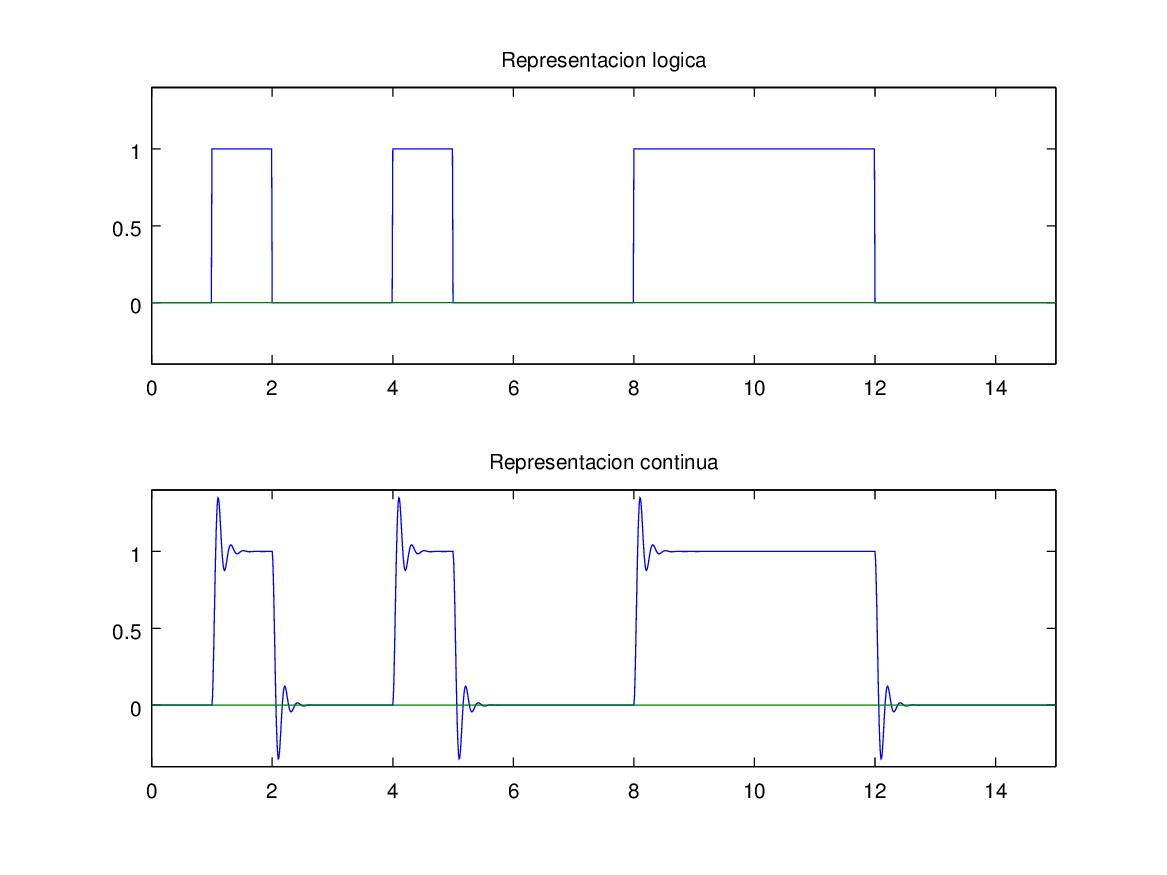
\includegraphics[height=3in]{./graphics/diversa.eps}
    \caption{Diversas representaciones de la misma se\~{n}al.}
    \label{diversaeps}
  \end{figure}

\item Consideremos ahora la funci\'{o}n de tiempo continuo
  \begin{equation}
    x\left(t\right) =\cos\left( 2 \, t\right), 
  \end{equation}
  Veamos su representaci\'{o}n en la Fig. (\ref{cos2tcoarseps}). Es
  evidente que en realidad tenemos secuencias de puntos, o sea
  se\~{n}ales de tiempo discreto, unidos por rectas de forma tal de
  dar la impresi\'{o}n de una se\~{n}al de de tiempo continuo cuando
  se la observa a una distancia adecuada.  Toda se\~{n}al procesada
  con una computadora es de tiempo discreto, porque las computadoras
  solo pueden procesar una cantidad finita y numerable de pedacitos de
  informaci\'{o}n (bits, en ingl\'{e}s). Lo que hacemos es graficar de
  forma tal que aceptamos lo que vemos como (un s\'{\i}mbolo de) una
  se\~{n}al de tiempo continuo.
  \begin{figure}
    \centering
    
\includegraphics[height=3in]{./py-graphics/target/cos2tcoarse.png}
    \caption{Es posible notar la discretizaci\'{o}n de esta
      funci\'{o}n ``continua''.}
    \label{cos2tcoarseps}
  \end{figure}
\end{enumerate}


%\subsection{Ejercicios para hacer}
%
%\begin{enumerate}
%\item En sus propias palabras, defina informaci\'{o}n, ruido, comunicaci\'{o}n, se\~{n}ales, sistemas, tiempo continuo, tiempo discreto, procesamiento, modelado, an\'{a}lisis, dise\~{n}o.
%
%\item De ejemplos de sistemas de tiempo continuo y discreto.
%
%\item \textquestiondown cual es la diferencia entre la informaci\'{o}n ``anal\'{o}gica'' (se\~{n}al de tiempo continuo) y la informaci\'{o}n ``digital'' (se\~{n}al de tiempo discreto)?
%\end{enumerate}

\section{Muestreo y cuantización}

El muestreo es la conversión de una señal de tiempo continuo $x(t)$ en una señal de tiempo discreto $x[n]$, tomando muestras de la señal en intervalos regulares de tiempo
\begin{equation}
	x[n] = x(n \, T_{s}).
\end{equation}
El muestreo se realiza para poder procesar la señal digitalmente, ya que la los sistemas digitales solo pueden trabajar con señales de tiempo discreto. El proceso de muestreo se realiza mediante un conversor analógico-digital (ADC), que toma muestras de la señal analógica a intervalos regulares $T_{s}$ (en el caso más común).

Además, los sistemas digitales necesitan que las señales esten cuantizadas.
La cuantización es la asignación de valores enteros a cada muestra y se realiza mediante un proceso de redondeo o truncamiento, que convierte los valores analógicos continuos (números reales) en valores discretos (números enteros en base 2). El nivel de cuantización se define por la cantidad de bits utilizados para representar cada muestra. Por ejemplo, una cuantización de $8$ bits produce $256$ posibles valores discretos para cada muestra.

Cabe aclarar que existen muestreos con intervalos $T_{s}$ variable o adaptivo.

\section{Propiedades de las se\~{n}ales}

\subsection{Se\~{n}ales acotadas y no acotadas de tiempo continuo}

Una se\~{n}al de tiempo continuo $x(t)$ es \textbf{acotada} si existe un n\'{u}mero real finito $M$ que
es mayor que el valor absoluto de $x(t)$ para todo valor de $t$
\begin{equation}
  |x(t)| < M,
\end{equation}

Una se\~{n}al de tiempo continuo $x(t)$ es \textbf{no acotada} si
existe $t_{1}$ tal que
\begin{equation}
  \begin{array}{c}
    Lim                     \\
    t \rightarrow t_{1}     
  \end{array}
  |x(t)| = \infty.
\end{equation}

\subsection{Se\~{n}ales acotadas y no acotadas de tiempo discreto}

Una se\~{n}al de tiempo discreto $x[n]$ es \textbf{acotada} si existe un n\'{u}mero real finito $M$ que
es mayor que el valor absoluto de $x[n]$ para todo valor de $n$
\begin{equation}
  |x[n]| < M,
\end{equation}.

Una se\~{n}al de tiempo discreto $x[n]$ es \textbf{no acotada} si
existe un tiempo $n_{1}$ tal que
\begin{equation}
  \begin{array}{c}
    Lim                     \\
    n \rightarrow n_{1}     
  \end{array}
  |x[n]| = \infty.
\end{equation}

\subsection{Se\~{n}ales infinitas y finitas, lateral derecha o lateral
  izquierda, causales y anticausales (tiempo continuo)}

Esto se refiere al momento en que las señales empiezan y terminan.

\begin{enumerate}
\item Una se\~{n}al $x(t)$ es finita si su valor es nulo antes de un
  tiempo de inicio $t_{1}$ y despu\'{e}s de un tiempo de
  finalizaci\'{o}n $t_{2}$. En caso contrario, la se\~{n}al es
  infinita.

\item Note que estas definiciones implican que para que una se\~{n}al
  sea infinita uno solo de ambos tiempos $t_{1}$ y $t_{2}$ necesita
  ser infinito mientras que el otro puede ser finito.
        
\item Una se\~{n}al $x(t)$ es infinita lateral derecho si $t_{2}
  \rightarrow \infty$ y $t_{1}$ tiene un valor finito.
        
\item Una se\~{n}al $x(t)$ es infinita lateral izquierdo si $t_{1}
  \rightarrow -\infty$ y $t_{2}$ tiene un valor finito.
        
\item Una se\~{n}al $x(t)$ es causal si es infinita lateral derecha y
  adem\'{a}s $t_{1} = 0$.
        
\item Una se\~{n}al $x(t)$ es nocausal si es infinita lateral
  izquierda y adem\'{a}s $t_{2} = 0$.

\item Note que una se\~{n}al puede ser infinita y acotada a la vez.
  Por ejemplo, $x(t) = cos(t)$.
\end{enumerate}

\subsection{Se\~{n}ales infinitas y finitas, lateral derecha o lateral
  izquierda, causales y anticausales (tiempo discreto)}

\begin{itemize}
\item Una se\~{n}al $x[n]$ es finita si su valor es nulo antes de un
  tiempo de inicio $n_{1}$ y despu\'{e}s de un tiempo de
  finalizaci\'{o}n $n_{2}$. En caso contrario, la se\~{n}al es
  infinita.

\item Note que estas definiciones implican que para que una se\~{n}al
  sea infinita uno solo de ambos tiempos $n_{1}$ y $n_{2}$ necesita
  ser infinito mientras que el otro puede ser finito.
        
\item Una se\~{n}al $x[n]$ es infinita lateral derecho si $n_{2}
  \rightarrow \infty$ y $n_{1}$ tiene un valor finito.
        
\item Una se\~{n}al $x[n]$ es infinita lateral izquierdo si $n_{1}
  \rightarrow -\infty$ y $n_{2}$ tiene un valor finito.
        
\item Una se\~{n}al $x[n]$ es causal si es infinita lateral derecha y
  adem\'{a}s $n_{1} = 0$.
        
\item Una se\~{n}al $x[n]$ es nocausal si es infinita lateral
  izquierda y adem\'{a}s $n_{2} = 0$.

\item Note que una se\~{n}al puede ser infinita y acotada a la vez.
  Por ejemplo, $x[n] = cos[n]$.
\end{itemize}

\subsection{Se\~{n}ales pares de tiempo continuo}

Una se\~{n}al de tiempo continuo es par si verifica la condici\'{o}n
\begin{equation}
  x(-t)=x(t).
\end{equation}

\subsubsection{Ejemplo}

Considere la siguiente ecuaci\'{o}n
\begin{equation}
  \cos (-t)=\cos (t).
\end{equation}
Vea la Fig. (\ref{contpareps}). Existe simetr\'{\i}a vertical, o
respecto al eje de absisas.

\begin{figure}
  \centering
  
\includegraphics[height=3in]{./py-graphics/target/contpar.png}
  \caption{Funci\'{o}n par (tiempo continuo)}
  \label{contpareps}
\end{figure}

\subsection{Se\~{n}ales pares de tiempo discreto}

Una se\~{n}al de tiempo discreto es par si verifica la condici\'{o}n
\begin{equation}
  x[-n]=x[n].
\end{equation}

\subsubsection{Ejemplo}

Considere la siguiente funci\'{o}n
\begin{equation}
  x[-n]=\frac{(-n)^{2}}{10}=\frac{n^{2}}{10}=x[n].
\end{equation}
Vea la Fig. (\ref{discpareps}). La gr\'{a}fica es invariante para una
rotaci\'{o}n de $\pi$ radianes.

\begin{figure}
  \centering
  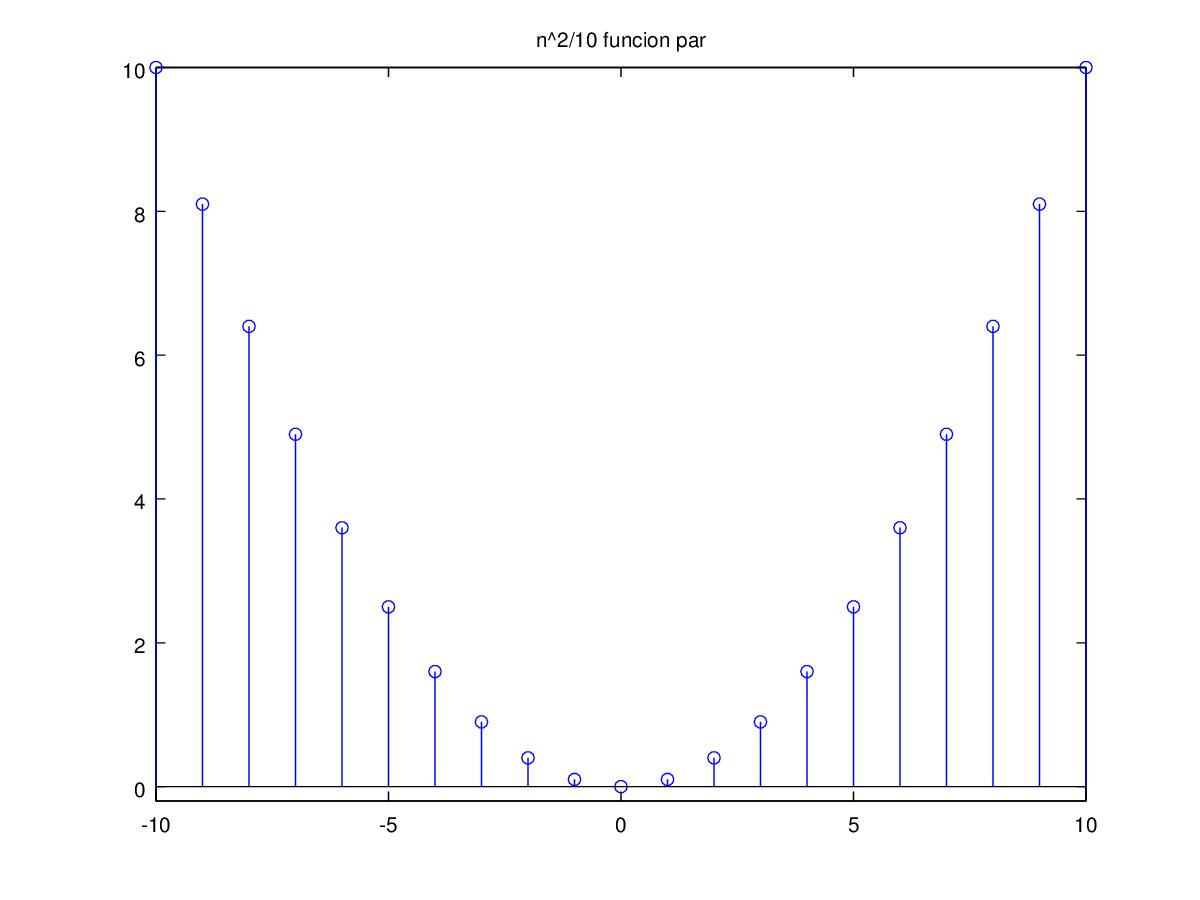
\includegraphics[height=3in]{./graphics/discpar.eps}
  \caption{Funci\'{o}n par (tiempo discreto). La gr\'{a}fica es
    invariante para una rotaci\'{o}n de $\pi$ radianes.}
  \label{discpareps}
\end{figure}

\subsection{Se\~{n}ales impares de tiempo continuo}

Una se\~{n}al de tiempo discreto es impar si verifica la condici\'{o}n
\begin{equation}
  x(-t)=-x(t).
\end{equation}

\subsubsection{Ejemplo}

Considere la siguiente funci\'{o}n
\begin{equation}
  \sin (-t)=-\sin (t).
\end{equation}
Vea la Fig. (\ref{contimpareps})

\begin{figure}
  \centering
  
\includegraphics[height=3in]{./py-graphics/target/contimpar.png}
  \caption{Funci\'{o}n impar (tiempo continuo)}
  \label{contimpareps}
\end{figure}

\subsection{Se\~{n}ales impares de tiempo discreto}

Una se\~{n}al de tiempo continuo es impar si verifica la condici\'{o}n
\begin{equation}
  x[-n]=-x[n].
\end{equation}

\subsubsection{Ejemplo}

Considere la siguiente funci\'{o}n
\begin{equation}
  x[-n]=\left( -n\right) ^{3}=-n^{3}=-x[n].
\end{equation}
Vea la Fig. (\ref{discimpareps}).

\begin{figure}
  \centering
  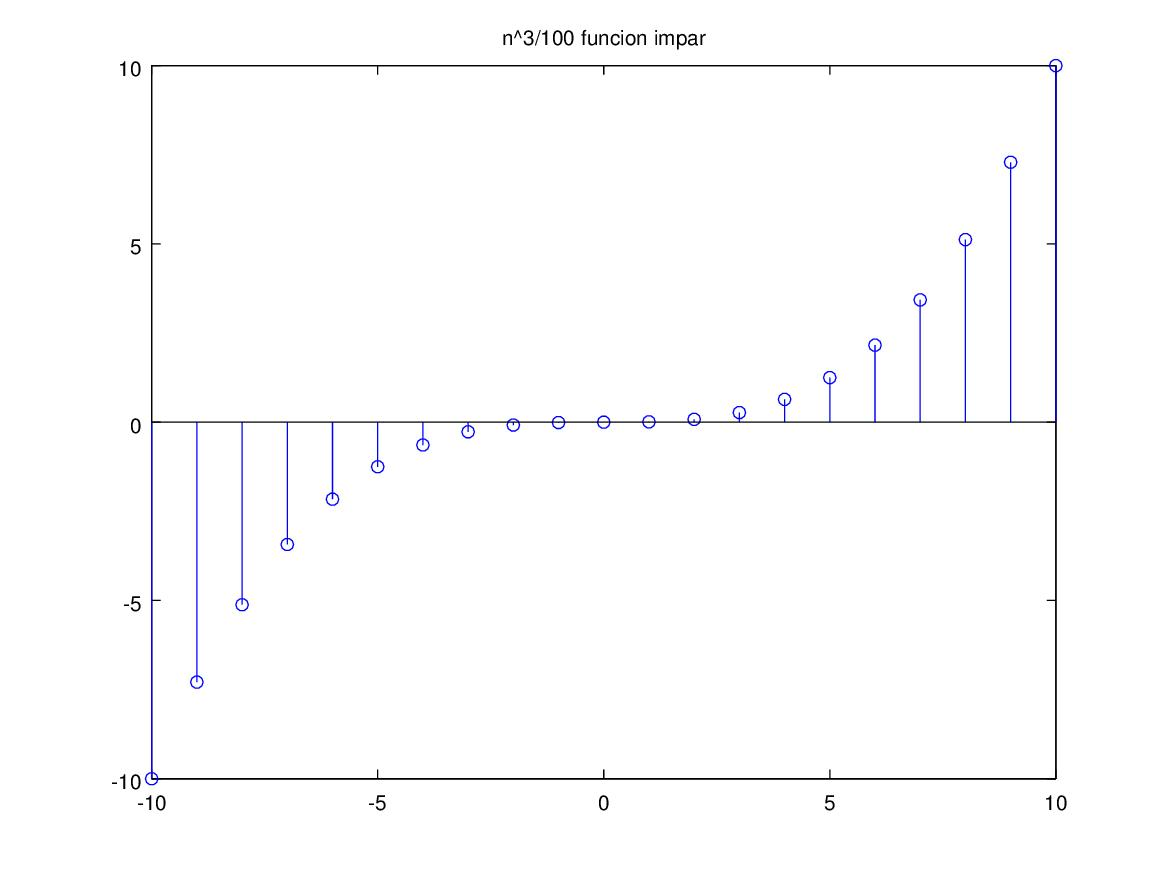
\includegraphics[height=3in]{./graphics/discimpar.eps}
  \caption{Funci\'{o}n impar (tiempo discreto)}
  \label{discimpareps}
\end{figure}

\subsection{Componentes par e impar de una se\~{n}al de tiempo
  continuo}

Una se\~{n}al de tiempo continuo puede descomponerse en componentes
par e impar
\begin{equation}
  x(t) = par(x(t)) + impar(x(t)),
\end{equation}
definiendo
\begin{eqnarray}
  par\left( x\left( t\right) \right) &=&\frac{1}{2}\left( x\left( t\right)
    +x\left( -t\right) \right) , \\
  impar\left( x\left( t\right) \right) &=&\frac{1}{2}\left( x\left( t\right)
    -x\left( -t\right) \right) .
\end{eqnarray}

\subsubsection{Ejemplo}

Vea la Fig. (\ref{contparimpareps}).

\begin{figure}
  \centering
  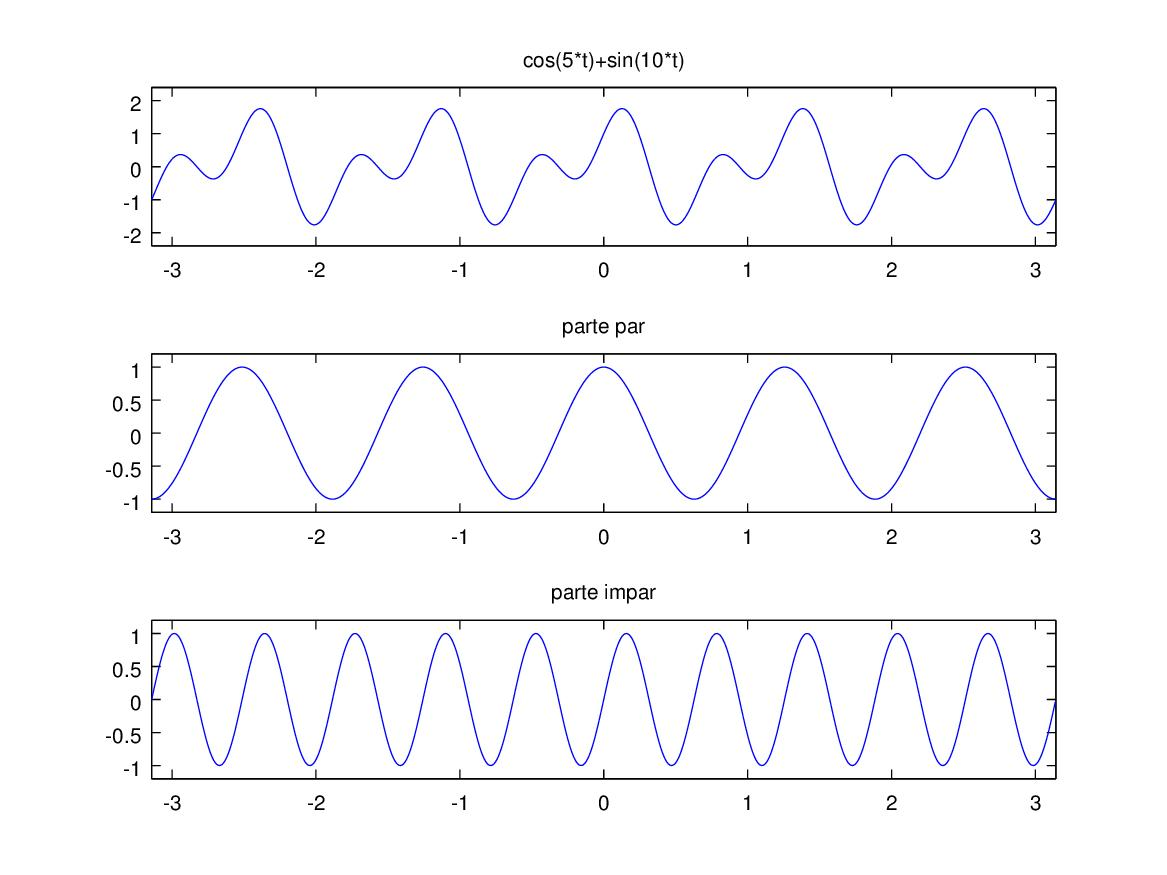
\includegraphics[height=3in]{./graphics/contparimpar.eps}
  \caption{Primer gr\'{a}fico: una funci\'{o}n con componentes pares e impares (tiempo continuo). Segundo gr\'{a}fico: componente par. Tercer gr\'{a}fico: componente impar. 
}
  \label{contparimpareps}
\end{figure}

\subsection{Componentes par e impar de una se\~{n}al de tiempo discreto}

Una se\~{n}al de tiempo discreto puede descomponerse en componentes
par e impar
\begin{equation}
  x[n] = par(x[n]) + impar(x[n]),
\end{equation}
definiendo
\begin{eqnarray}
  par\left( x\left[ n\right] \right) &=&
  \frac{1}{2}\left( x\left[ n\right] +x\left[ -n\right] \right) , \\
  impar\left( x\left[ n\right] \right) &=&
  \frac{1}{2}\left( x\left[ n\right] -x\left[ -n\right] \right) .
\end{eqnarray}

\subsubsection{Ejemplo}
Vea la Fig. (\ref{discparimpareps}).

\begin{figure}
  \centering
  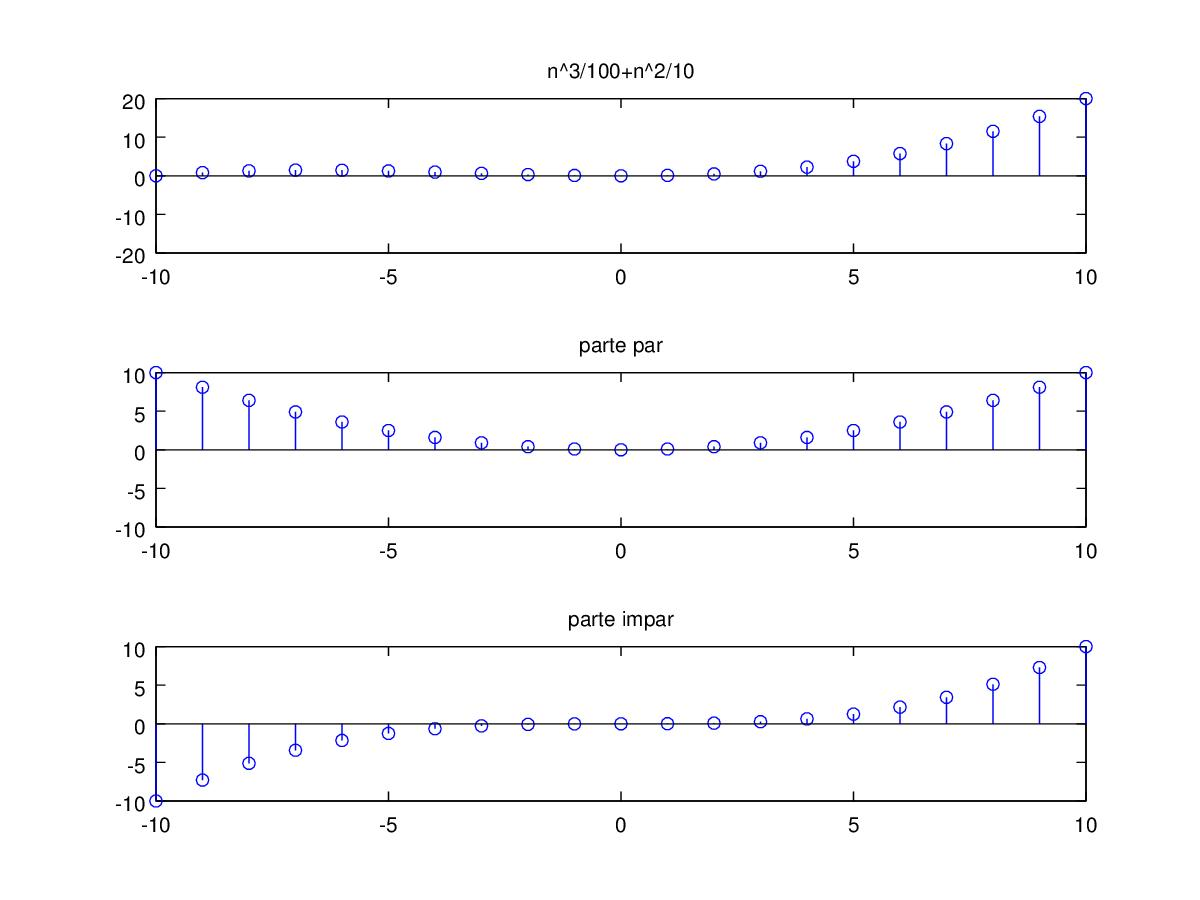
\includegraphics[height=3in]{./graphics/discparimpar.eps}
  \caption{Primer gr\'{a}fico: una funci\'{o}n con componentes pares e impares (tiempo discreto). Segundo gr\'{a}fico: componente par. Tercer gr\'{a}fico: componente impar.} 
  \label{discparimpareps}
\end{figure}

% \subsection{Ejercicios para hacer}
% Para cada uno de los tipos de se\~{n}ales considerados en esta secci\'{o}n de una definici\'{o}n y dos ejemplos con gr\'{a}ficos realizados en Matlab.

\section{Se\~{n}ales peri\'{o}dicas}

\subsection{Definici\'{o}n de per\'{\i}odo (tiempo continuo)}

Una se\~{n}al de tiempo continuo es peri\'{o}dica si existe un
n\'{u}mero $T$ denominado per\'{\i}odo tal que
\begin{equation}
  x(t)=x\left( t+ k \, T\right),
\end{equation}
donde $k$ es un número entero.

\subsection{Definici\'{o}n de per\'{\i}odo (tiempo discreto)}

Una se\~{n}al de tiempo discreto es peri\'{o}dica si existe un
n\'{u}mero $N$ denominado per\'{\i}odo tal que
\begin{equation}
  x[n]=x[n+ k \, N],
\end{equation}
donde $k$ es un número entero.

\subsection{Ejemplos}

\begin{enumerate}
\item Vea la Fig. (\ref{perconteps}). El per\'{\i}odo es $T = 10$.

\item Vea la Fig. (\ref{perdisceps}). El per\'{\i}odo es $N = 10$.

\item Vea la Fig. (\ref{noperdisceps}). No existe un n\'{u}mero $N$ tal que
\begin{equation}
  x[n]=x[n+N].
\end{equation}
Esta se\~{n}al nos parece peri\'{o}dica porque puede dibujarse sobre
una se\~{n}al peri\'{o}dica de tiempo continuo, denominada envolvente.
\end{enumerate}

\begin{figure}
  \centering
  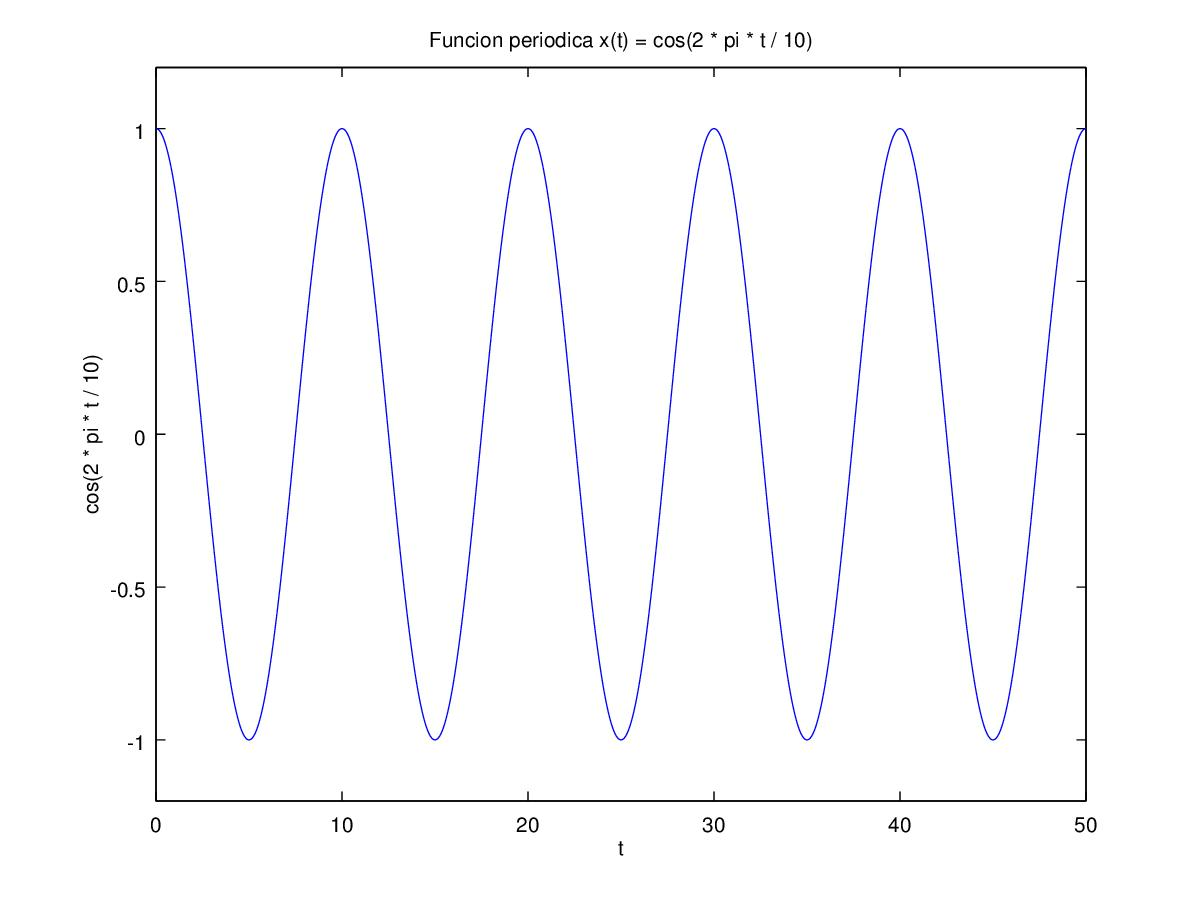
\includegraphics[height=3in]{./graphics/percont.eps}
  \caption{Se\~{n}al peri\'{o}dica de tiempo continuo $T = 10$}
  \label{perconteps}
  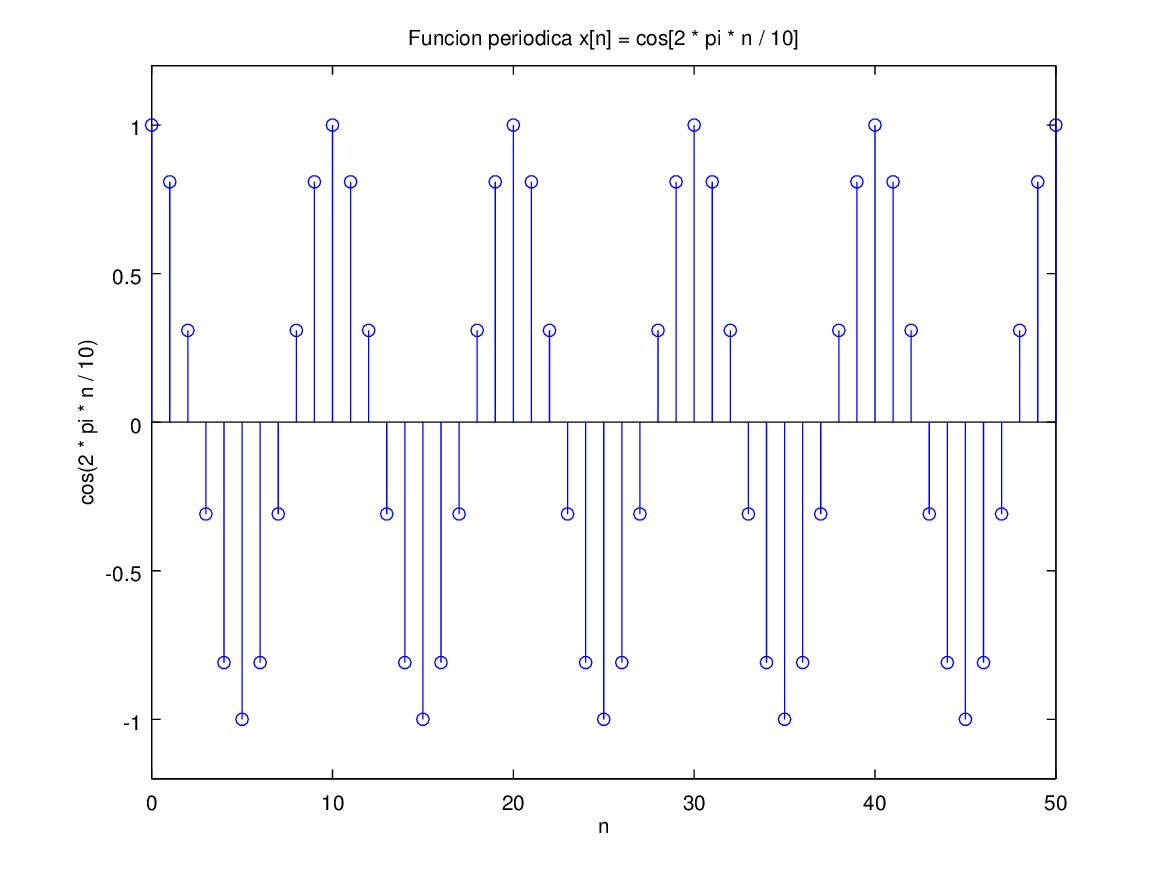
\includegraphics[height=3in]{./graphics/perdisc.eps}
  \caption{Se\~{n}al peri\'{o}dica de tiempo discreto $N = 10$}
  \label{perdisceps}
\end{figure}

\begin{figure}
  \centering
  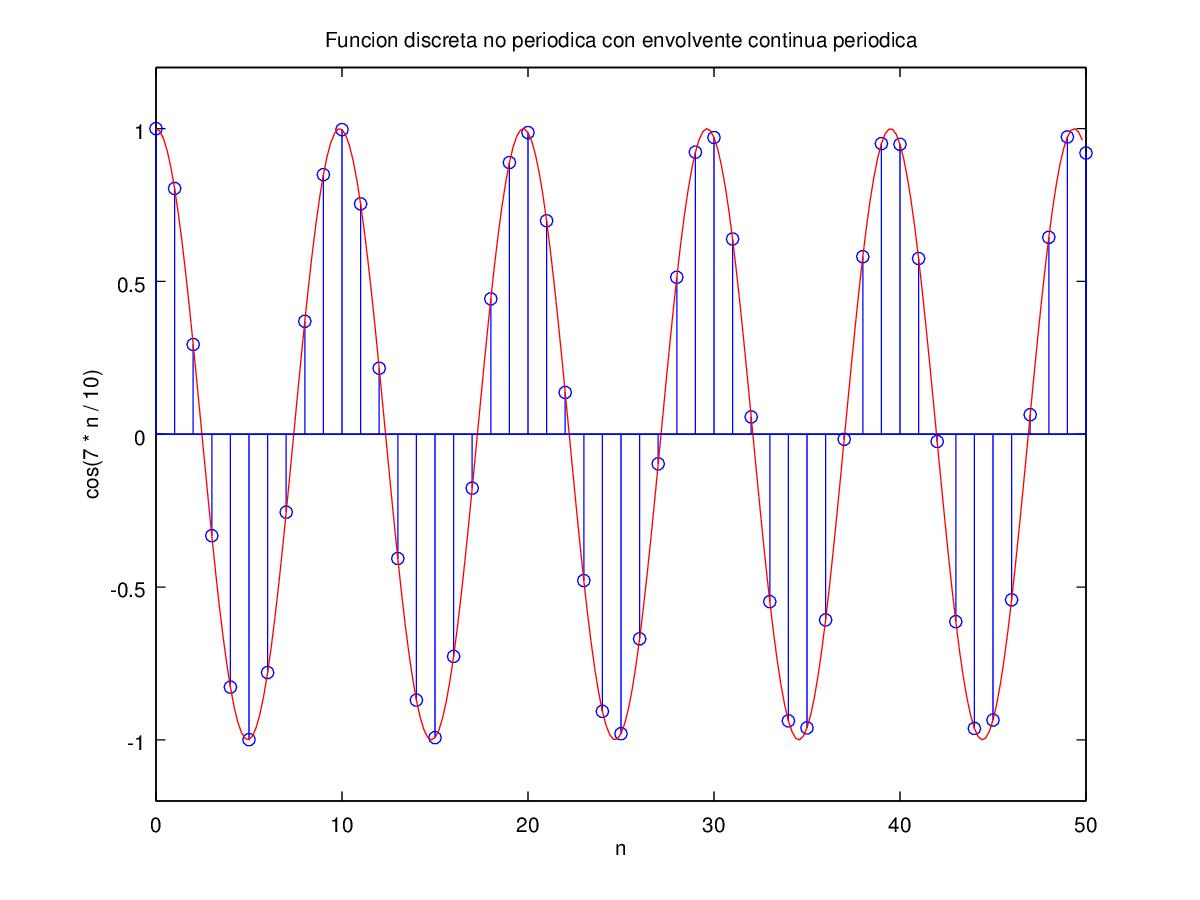
\includegraphics[height=3in]{./graphics/noperdisc.eps}
  \caption{Se\~{n}al de tiempo discreto que \textbf{NO} es
    peri\'{o}dica y que tiene una envolvente continua que si es
    peri\'{o}dica}
  \label{noperdisceps}  
\end{figure}

\subsection{Como encontrar los períodos de señales periódicas de tiempo continuo}

Las señales periódicas de tiempo continuo $x_{c}(t) = cos(\omega_{0} \, t)$ y
$x_{s}(t) = sin(\omega_{0} \, t)$ verifican la igualdad
\begin{equation}
 \omega_{0} \, T = 2 \, \pi.
\end{equation}
Por lo tanto $T = \frac{2 \, \pi}{\omega_{0}}$. 

\subsubsection{Ejemplos}

\begin{enumerate}
\item  $x\left( t\right) = 4 \, \cos \left( 5 \, \pi \, t\right),$ donde $\omega_{0} = 5 \, \pi$.
Podemos calcular el período
\begin{equation}
    5 \, \pi \, T= 2 \, \pi , \qquad T=\frac{2}{5}, \qquad \cos \left( 5 \, \pi \, \frac{2}{5}\right) = 
    \cos \left( 2 \, \pi \right) = \cos \left( 0\right) .
\end{equation}

\item  $x\left( t\right) =4\cos \left( 4 \, \pi \, t-\frac{\pi }{4}\right).$ Podemos calcular el período
\begin{equation}
    4 \, \pi \, T= 2 \, \pi , \qquad T=\frac{1}{2}, \qquad \cos \left( 4\pi \frac{1}{2} - \frac{\pi}{4}\right) = 
    \cos \left( 2 \, \pi - \frac{\pi}{4}\right) = \cos \left( -\frac{\pi}{4}\right) .
\end{equation}

\item  $x\left( t\right) =u\left( t\right) +4 \, \cos \left( 5 \, \pi \, t\right),$ 
no es periódica, porque 
\begin{equation}
u\left(\frac{-2}{5}\right) - 4 \, \cos \left(-5 \, \pi \, \frac{2}{5}\right) \neq u\left(\frac{2}{5}\right) - 4 \, \cos \left(5 \, \pi \, \frac{2}{5}\right). 
\end{equation}


\item  $x\left( t\right) =u\left( t\right) -\frac{1}{2}.$ No es periódica.

\item  $x\left[ n\right] =4\cos \left( \pi \, n\right).$ En este caso veremos que debe cumplirse 
\begin{equation}
\pi \, N=2 \, \pi , N=2.
\end{equation}

\item  $x\left[ n\right] =4\sin \left( 3 \, n\right).$ En  este caso veremos que $3 \, N \neq 2 \, \pi$. Por lo tanto $x[n]$ no es periódica.

\item  $x\left[ n\right] =4\cos \left( \pi n-2\right),$ es periódica con $N = 2$.

\item  $x\left[ n\right] =\left( -1\right) ^{n}$ es periódica con $N = 2$.

\end{enumerate}

% \subsection{Ejercicios para hacer}
% 
% \textquestiondown Cu\'{a}l es la se\~{n}al peri\'{o}dica de tiempo discreto que var\'{\i}a m\'{a}s rapidamente? \textquestiondown y
% m\'{a}s lentamente?
% 
% Escriba y grafique al menos dos funciones peri\'{o}dicas de distinta frecuencia (tiempo discreto).

\section{Se\~{n}ales exponenciales}

\subsection{Repaso de n\'{u}meros complejos}

Vamos a considerar distintos conceptos en los cuales emplearemos
n\'{u}meros complejos.  Por lo tanto, nos conviene recordar ciertas
notaciones y operaciones.

\subsubsection{Unidad imaginaria}

Definimos la unidad imaginaria como
\begin{equation}
  j = \sqrt{-1}.
\end{equation}
Por lo tanto, cumple con la igualdad
\begin{equation}
  j^{2} = -1.
\end{equation}

\subsubsection{N\'{u}meros complejos}

El conjunto de los n\'{u}meros complejos se simboliza $C$ y sus
elementos se representan en forma cartesiana como $a + b \, j$,
donde $a \in R$, $b \in R$, y $j$ es la unidad imaginaria.

\subsubsection{N\'{u}meros complejos conjugados}

Llamamos n\'{u}meros complejos conjugados a un par de n\'{u}meros que
simbolizamos $z$ y $\overline{z}$
\begin{equation}
  \begin{array}{ll}
    z =             &       a + j b,                        \\
    & \\
    \overline{z}    =       &       \overline{a + j b} = a - j b,
  \end{array}
\end{equation}
donde $a \in R$, $b \in R$, y $j$ es la unidad imaginaria.

\subsubsection{Parte real de un n\'{u}mero complejo}

Definimos a la funci\'{o}n parte real de un n\'{u}mero complejo como
\begin{equation}
  \Re{ \left( a + j b \right)} = a.
\end{equation}
Es sencillo deducir la propiedad
\begin{equation}
  \Re{ \left( a + j b \right)} = 
  \frac{(a + j b) + \overline{(a + j b)}}{2} =  \frac{(a + j b) + (a - j b)}{2} = a.
\end{equation}

\subsubsection{Parte imaginaria de un n\'{u}mero complejo}

Definimos a la funci\'{o}n parte imaginaria de un n\'{u}mero complejo
como
\begin{equation}
  \Im{\left( a + j b \right)} = b.
\end{equation}
Es sencillo deducir la propiedad
\begin{equation}
  \Im{ \left( a + j b \right)} = 
  \frac{(a + j b) - \overline{(a + j b)}}{2 j} =  \frac{(a + j b) - (a - j b)}{2 j} = b.
\end{equation}

\subsubsection{M\'{o}dulo de un n\'{u}mero complejo}

Definimos a la funci\'{o}n m\'{o}dulo de un n\'{u}mero complejo como
\begin{equation}
  \| a + j b \| = \sqrt{\left(a + j b\right)\left(a - j b\right)} = \sqrt{ a^{2} + b^{2}}.
\end{equation}
Por su definici\'{o}n, es un n\'{u}mero real igual o mayor que $0$.

\subsubsection{Fase de un n\'{u}mero complejo}

Definimos a la funci\'{o}n fase de un n\'{u}mero complejo como
\begin{equation}
  \angle a + j b  = \arctan (\frac{b}{a}).
\end{equation}

\subsubsection{Exponencial compleja}

Definimos la funci\'{o}n exponencial compleja como
\begin{equation}
  e^{a + j \, b} = e^{a} \, e^{j \, b} = e^{a} \, \left( \cos (b) + j \, \sin (b) \right),
\end{equation}

\subsubsection{Relaci\'{o}n de Euler}

La relaci\'{o}n de Euler es la igualdad
\begin{equation}
  e^{j b} =  \cos \left( b \right) + j \, \sin\left( b \right), \label{expeuler}
\end{equation}
Por lo tanto podemos escribir
\begin{equation}
  \cos \left( b \right) = \frac{e^{j \, b}+e^{-j \, b}}{2}, \label{coseuler}
\end{equation}
y
\begin{equation}
  \sin \left( b \right) = \frac{e^{j \, b}-e^{-j \, b}}{2j}. \label{sineuler}
\end{equation}


\subsubsection{Representaci\'{o}n en forma polar}

Un n\'{u}mero complejo $a + j b$ puede representarse en forma polar
\begin{equation}
  a + j b = \| a + j b\| e^{ j \, \angle{ a + j \, b} }.
\end{equation}

\subsection{Se\~{n}ales exponenciales de tiempo continuo}

Las se\~{n}ales exponenciales de tiempo continuo son las que tienen la
forma
\begin{equation}
  x(t)=R \, e^{a \, t}.
\end{equation}

\subsubsection{Se\~{n}ales exponenciales reales de tiempo continuo}

Se dice que la se\~{n}al exponencial es real si $R\in \Re$ y $a\in \Re$.

Si $ a > 0,$ entonces la se\~{n}al exponencial crece a medida que $t$ crece.

Si $ a < 0,$ entonces la se\~{n}al exponencial decrece a medida que $t$ crece.

\subsubsection{Se\~{n}ales exponenciales imaginarias de tiempo continuo}

Si $a = j \omega_{0}$ donde $j=\sqrt{-1}$ puede aplicarse la
relaci\'{o}n de Euler
\begin{equation}
  x\left( t\right) = 
  R \, e^{j \, \omega_{0} \, t}= 
  R \, \left(\cos \left( \omega_{0} \, t\right) +j \, \sin\left( \omega_{0} \, t\right) \right).
\end{equation}

\subsubsection{Se\~{n}ales exponenciales complejas de tiempo continuo}

La exponencial es compleja si $R$ es un n\'{u}mero real y $a$ es un n\'{u}mero complejo
\begin{equation}
  R\in \Re,
\end{equation}
y
\begin{equation}
  a=\gamma+j \, \omega_{0}\in C.
\end{equation}
La exponencial compleja puede evaluarse con la relaci\'{o}n de Euler
\begin{equation}
  x(t)= R \, e^{\gamma \, t}e^{j \, \omega_{0} \, t} = 
  R \, e^{\gamma \, t}\left( \cos \left( \omega_{0} \, t\right) + j \, \sin \left( \omega_{0} \, t\right) \right) ,
\end{equation}
donde
\begin{itemize}
\item $j=\sqrt{-1}$ es la unidad imaginaria
\item $R \, e^{\gamma \, t}$ es la envolvente,
\item Per\'{\i}odo $T$ y frecuencia $\omega_{0} = \frac{2 \, \pi}{T}$.
\end{itemize}

\subsubsection{Se\~{n}ales exponenciales generalizadas de tiempo continuo}
La exponencial es generalizada si tanto $R$ como $a$ son n\'{u}meros complejos
\begin{eqnarray}
  R &=&\alpha \, e^{j \, \theta }, \\
  a &=&\gamma + j \, \omega_{0}.
\end{eqnarray}
Podemos escribir entonces aplicando la relaci\'{o}n de Euler
\begin{equation}
  x\left( t\right) = R \, e^{a \, t}=
  \alpha \, e^{j \, \theta } \, e^{(\gamma + j \, \omega_{0}) \, t} = 
  \alpha \, e^{j \, \theta } \, e^{\gamma \, t} \, e^{j \, \omega_{0} \, t},
\end{equation}
\begin{equation}
  x\left( t\right) = R \, e^{a \, t}=
  \alpha \, e^{j \, \theta } \, e^{(\gamma + j \, \omega_{0}) \, t} = 
  \alpha \, e^{\gamma \, t} \, e^{j \, (\omega_{0} \, t + \theta)},
\end{equation}
\begin{equation}
  x\left( t\right) = R \, e^{a \, t}=
  \alpha \, e^{\gamma t}
  \left( \cos \left( \omega_{0} \, t+\theta \right) +
    j \, \sin \left( \omega_{0} \, t+\theta \right) \right) ,
\end{equation}
donde
\begin{itemize}
\item $j=\sqrt{-1}$ es la unidad imaginaria,
\item $\alpha e^{\gamma t}$ es la envolvente,
\item $\theta$ es la fase,
\item $\omega_{0}$ la frecuencia.
\end{itemize}

\subsection{Propiedades de la se\~{n}al exponencial imaginaria de tiempo continuo}

\subsubsection{Per\'{\i}odo y frecuencia}

Consideremos una se\~{n}al peri\'{o}dica de tiempo continuo con período $T_{0}$
\begin{equation}
  x\left( t\right) = x\left( t+T_{0}\right) .
\end{equation}
Para verificar que una se\~{n}al exponencial imaginaria de tiempo continuo sea
peri\'{o}dica podemos factorear
\begin{equation}
  R \, e^{j \, \omega_{0} \, t}= 
  R \, e^{j \, \omega_{0} \, \left(t+T_{0}\right)}= 
  R \, e^{j \, \omega_{0} \, t} \, e^{j \, \omega_{0} \, T_{0}},
\end{equation}
Aplicando la relación de Euler, verificamos
\begin{equation}
  e^{j \, \omega_{0} \, T_{0}}=
  \cos \left( \omega_{0} \, T_{0}\right) +
  j \, \sin \left(\omega_{0} \, T_{0}\right) = cos(2 \, \pi) + j \, sin(2 \, \pi) = 1,
\end{equation}
y
\begin{equation} 
  T_{0} = \frac{2 \, \pi }{\left|\omega_{0}\right| }.
\end{equation}
La conclusi\'{o}n es que la se\~{n}al exponencial imaginaria de tiempo
continuo \textbf{siempre} es peri\'{o}dica porque siempre podemos
encontrar $T_{0}$ dado $\omega_{0}$.

\subsubsection{Funciones arm\'{o}nicas de tiempo continuo} 

Dada una se\~{n}al peri\'{o}dica
\begin{equation}
  x(t) = x(t + T),
\end{equation}
existen infinitas se\~{n}ales peri\'{o}dicas arm\'{o}nicas de frecuencia $\omega_{k} = k \, \omega_{0} = k \, \frac{2 \, \pi}{T}$,
y período $T_{k} = \frac{T_{0}}{k}$, para $k \in N$, $k > 0$.


\subsection{Se\~{n}ales exponenciales de tiempo discreto}

Consideremos ahora la se\~{n}al exponencial de tiempo discreto
\begin{equation}
  x\left[ n\right] = R \, e^{\beta \, n} = R \, \alpha^{n},
\end{equation}
donde definimos
\begin{equation}
  \alpha = e^{\beta}.
\end{equation}

\subsubsection{Se\~{n}ales exponenciales reales de tiempo discreto}

\begin{enumerate}
\item Decimos que la exponencial es real si 
$\alpha \in \Re$ y $\beta \in \Re$.

\item Si $\left| \alpha \right| >1,$ o sea $\beta >0,$ entonces la
  exponencial crece a medida que $n$ crece.

\item Si $\left| \alpha \right| <1,$ o sea $\beta <0,$ entonces la
  exponencial decrece a medida que $n$ crece.
\end{enumerate}

\subsubsection{Se\~{n}ales exponenciales imaginarias de tiempo discreto}

Si $\beta $ es un n\'{u}mero imaginario puro entonces 
$\alpha = e^{j \, \omega_{0}} \rightarrow \left| \alpha \right| =1,$ y por la relaci\'{o}n de Euler
\begin{equation}
  x\left[ n\right] = 
  e^{j \, \omega_{0} \, n}=
  \cos \left( \omega_{0} \, n\right) +j \, \sin\left( \omega_{0} \, n\right).
\end{equation}

\subsubsection{Se\~{n}ales exponenciales generalizadas de tiempo discreto}

Definimos a la se\~{n}al exponencial generalizada de tiempo discreto
como
\begin{equation}
  x\left[ n\right] = R \, \alpha^{n},
\end{equation}
donde
\begin{eqnarray}
  R &=&\left| R \, \right| e^{j\theta }, \\
  \alpha &=&\left| \alpha \right| \, e^{j \, \omega_{0}}.
\end{eqnarray}
Podemos escribir entonces
\begin{equation}
  x\left[ n\right] =R \, \alpha^{n}=
  \left| R \, \right| \left| \alpha \right|^{n} \, e^{j \, \theta } \, e^{j \, \omega_{0} \, n} = 
  \left| R \, \right| \left| \alpha \right|^{n} \, e^{j \, (\omega_{0} \, n + \theta)},
\end{equation}
y
\begin{equation}
  x\left[ n\right] =R \, \alpha^{n}=
  \left| R \, \right| \left| \alpha \right|^{n} \, 
  \left( \cos \left( \omega_{0} \, n+\theta \right) +j \, \sin\left(\omega_{0} \, n+\theta \right) \right) .
\end{equation}

\subsection{Propiedades de la se\~{n}al exponencial imaginaria de tiempo discreto}

\subsubsection{Per\'{\i}odo y frecuencia}

Supongamos una funci\'{o}n exponencial imaginaria de tiempo discreto que
tenga per\'{\i}odo $N$
\begin{equation}
 x[n] = x[n + N].
\end{equation}
Por lo tanto, debería ser
\begin{equation}
 e^{j \, \omega_{0} \, n} = e^{j \, \omega_{0} \, (n + N)}.
\end{equation}
Esto significa que $\omega_{0}$ cumple con la relaci\'{o}n
\begin{equation}
  e^{j \, \omega_{0}\left( n+N\right) }=
  e^{j \, \omega_{0} \, n} \, e^{j \, \omega_{0} \, N}=e^{j \, \omega_{0} \, n}
  \Leftrightarrow e^{j \, \omega_{0} \, N}=1\Leftrightarrow\omega_{0} \, N=2 \, \pi M,
\end{equation}
donde $M$ es un n\'{u}mero entero. 
Por lo tanto, el per\'{\i}odo debe ser
\begin{equation}
  N =\frac{2 \, \pi }{\omega_{0}} \, M.
\end{equation}
Entonces si $\omega_{0} = P \, 2 \, \pi$, donde $P$ es un número racional,
\begin{equation}
  N =\frac{2 \, \pi }{P \, 2 \, \pi} \, M = \frac{M}{P},
\end{equation}
y
\begin{equation}
  P = \frac{M}{N}.
\end{equation}

\textbf{Para que una exponencial imaginaria de tiempo discreto sea
  peri\'{o}dica, su frecuencia debe ser una fracci\'{o}n propia de
  $\pi$.}

\subsubsection{Igualdad entre se\~{n}ales exponenciales con frecuencias $\omega_{0}$ y $\omega_{0}+2 \, \pi $}

Consideremos la funci\'{o}n $e^{j\left( \omega_{0}+2 \, \pi \right) n}$
que puede ser simplificada de la siguiente forma
\begin{equation}
  e^{j\left( \omega_{0}+2 \, \pi \right) \, n} = 
  e^{j \, \omega_{0} \, n} \, e^{j \, 2 \, \pi n} = 
  e^{j \, \omega_{0} \, n},
\end{equation}
porque
\begin{equation}
  e^{j2 \, \pi \, n}=
  \cos \left( 2 \, \pi \, n\right) +j \, \sin \left(2 \, \pi \, n\right) = 1+j \, 0, \forall n \in -2,-1,0,1,2,....
\end{equation}
Esto significa que dos funciones exponenciales complejas de tiempo discreto de frecuencias que difieran en $2 \, \pi $ son iguales.

\subsubsection{Señales armónicas de tiempo discreto}

Dada una se\~{n}al peri\'{o}dica
\begin{equation}
  x[n] = x[n + N],
\end{equation}
existen a lo sumo $N$ se\~{n}ales peri\'{o}dicas arm\'{o}nicas de frecuencia $\omega_{k} = k \, \frac{2 \, \pi}{N}$ 
enumerables $0 \leq k < N$, porque sino fuera así, $\omega_{k + N} = \omega_{k} + 2 \, \pi$.

Por ejemplo, consideremos
\begin{equation}
	x[n]_{k} = e^{j \, k \, \frac{2 \, \pi \, M}{N}}.
\end{equation}
Supongamos ahora que $k = N + 1$. Entonces
\begin{equation}
	x[n]_{N+1} = e^{j \, (N + 1) \, \frac{2 \, \pi \, M}{N}} = e^{j \, N \, \frac{2 \, \pi \, M}{N}} \, e^{j \, \frac{2 \, \pi \, M}{N}} = 
	e^{j \, \frac{2 \, \pi \, M}{N}} = x[n]_{1},
\end{equation}
porque $e^{j \, N \, \frac{2 \, \pi \, M}{N}} = e^{j \, 2 \, \pi \, M} = 1.$

\subsection{La se\~{n}al exponencial imaginaria es el bloque constructivo de otras se\~{n}ales peri\'{o}dicas}

\begin{enumerate}
\item Para construir otras se\~{n}ales peri\'{o}dicas usaremos
  conjuntos de exponenciales imaginarias (o sea, varias se\~{n}ales exponenciales imaginarias) a las que simbolizaremos
  \begin{equation}
    \phi _{k}\left( t\right) .
  \end{equation}
        
\item Usaremos exponenciales complejas $\phi_{k}(t)$ arm\'{o}nicas con un per\'{\i}odo com\'{u}n $T_{0}$.
  
\item
  Definiendo la frecuencia fundamental
  \begin{equation}
    \omega_{0}=\frac{2 \, \pi }{T_{0}},
  \end{equation}
  podemos definir el conjunto de funciones arm\'{o}nicas
  \begin{equation}
    \phi _{k}\left( t\right) = e^{j \, k \, \omega_{0} \, t}, k=0,\pm 1,\pm 2,....
  \end{equation}
        
\item Con la definici\'{o}n de funci\'{o}n arm\'{o}nica dada en el
  punto $2$ podemos construir funciones peri\'{o}dicas escritas como
  sumatorias de exponenciales imaginarias (multiplicadas por coeficientes adecuados).

\item Para obtener funciones peri\'{o}dicas escritas como combinaciones lineales
  de funciones trigonom\'{e}tricas podemos usar las relaciones
  \begin{equation}
    \cos \left(a \, t \right) = \frac{e^{j \, a \, t} + e^{-j \, a \, t}}{2},
  \end{equation}
  y
  \begin{equation}
    \sin \left(a t \right) = \frac{e^{j \, a \, t} - e^{-j \, a \, t}}{2 \, j}.
  \end{equation}

\end{enumerate}

\subsubsection{Ejemplo}

Consideremos la se\~{n}al
\begin{equation}
  x(t)= e^{j2t} + e^{-j2t} + j e^{j3t} - j e^{-j3t},      \label{ejeperiodicauno}
\end{equation}
equivalente a
\begin{equation}
  x(t)= 2 \, \frac{e^{j \, 2 \, t} + e^{-j \, 2 \, t}}{2} + (2 \, j) \, j \, \frac{(e^{j \, 3 \, t} - e^{-j \, 3 \, t})}{2 \, j},
\end{equation}
y finalmente a
\begin{equation}
  x(t)= 2 \, \cos \left(2 \, t \right) - 2 \, \sin \left(3 \, t \right). \label{ejeperiodicados}
\end{equation}
Observe que como los sumandos de (\ref{ejeperiodicauno}) son complejos
conjugados, $x(t)$ resulta ser una funci\'{o}n real, como vemos en
(\ref{ejeperiodicados}).

\subsection{Comparaci\'{o}n de las se\~{n}ales peri\'{o}dicas de tiempo continuo y discreto}

\subsubsection{Se\~{n}al de tiempo continuo $e^{j \, \protect\omega_{0} \, t}$}

\begin{enumerate}
\item Distintas se\~{n}ales para distintos valores de $\omega_{0};$

\item Peri\'{o}dica para cualquier valor de $\omega_{0};$

\item Frecuencia fundamental $\omega_{0};$

\item Per\'{\i}odo fundamental $T = \frac{2 \, \pi}{\omega_{0}}.$
\end{enumerate}

\subsubsection{Se\~{n}al de tiempo discreto $e^{j \, \protect\omega_{0}n}$}

\begin{enumerate}
\item Id\'{e}nticas se\~{n}ales para $\omega_{0}$ y $\omega_{0}+2 \, \pi
  ;$

\item Peri\'{o}dica s\'{o}lo si $\omega_{0} \, N=2 \, \pi \, M,$ y $N$ y $M$ sin
  factores en com\'{u}n;

\item Frecuencia fundamental $\omega_{0};$

\item Per\'{\i}odo fundamental $N$ tal que $\frac{N}{M} = \frac{2 \, \pi }{\omega_{0}}.$
\end{enumerate}

% \subsection{Ejercicios para hacer}
% 
% Escriba ejemplos gr\'{a}ficos en Matlab de se\~{n}ales peri\'{o}dicas de tiempo continuo y discreto.

\section{Se\~{n}ales singulares}

A continuaci\'{o}n veremos unos objetos matem\'{a}ticos especiales que
nos permiten representar ciertas \textbf{se\~{n}ales singulares}, y
as\'{\i} desarrollar una teor\'{\i}a matem\'{a}tica \'{u}til.

\subsection{El impulso unitario (tiempo discreto)}

Se define el impulso unitario de tiempo discreto como
\begin{equation}
  \delta \left[ n\right] =\left\{ 
    \begin{array}{ll}
      0, & n\neq 0, \\ 
      1, & n=0.
    \end{array}
  \right.                \label{impunidiscdef}
\end{equation}
Vea la Fig. (\ref{impunidisceps}).

\begin{figure}
  \centering
  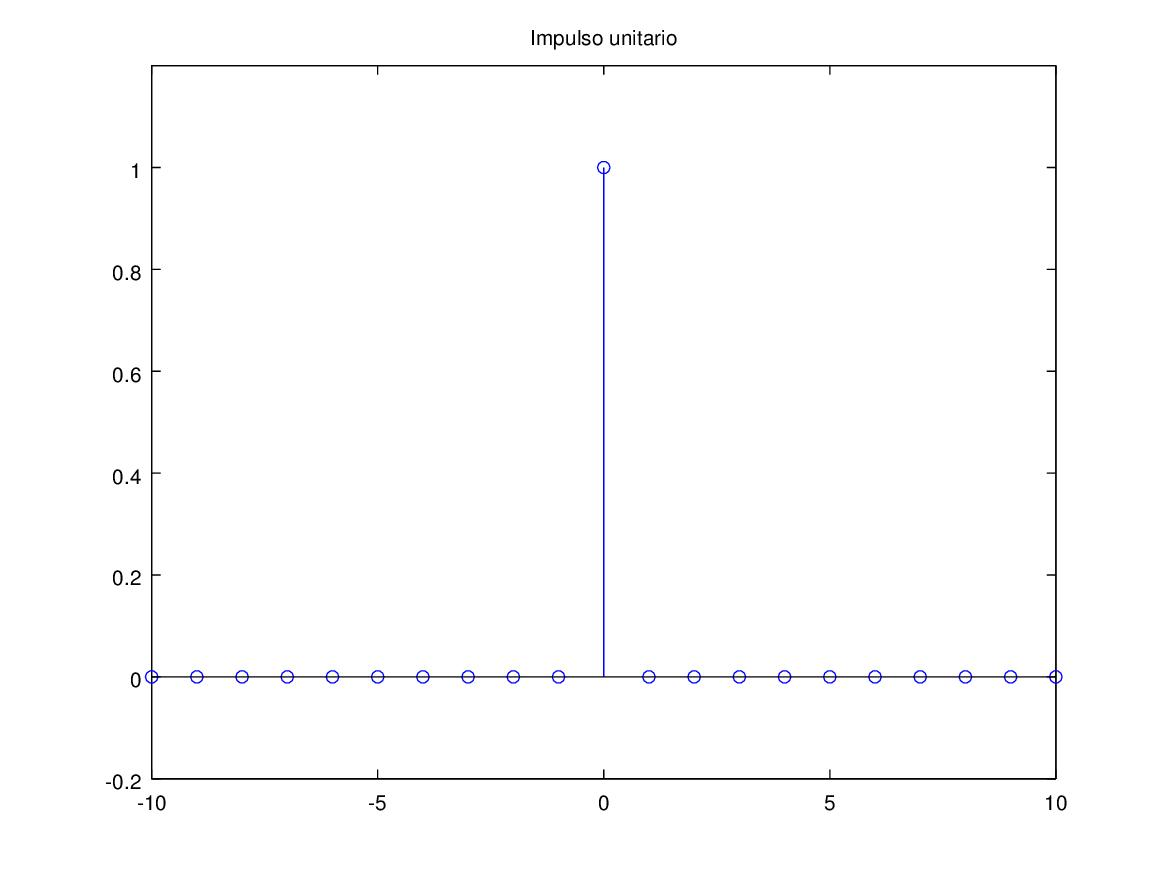
\includegraphics[height=3in]{./graphics/impunidisc.eps}
  \caption{Impulso unitario de tiempo discreto.}
  \label{impunidisceps}
\end{figure}

Podemos desplazar al impulso unitario en el tiempo. En este caso la
definici\'{o}n es
\begin{equation}
  \delta \left[ n - n_{0}\right] =\left\{ 
    \begin{array}{ll}
      0,      & n\neq n_{0}, \\ 
      1,      & n= n_{0}.
    \end{array}
  \right.
\end{equation}
Vea la Fig. (\ref{impunidiscdespeps}).

\begin{figure}
  \centering
  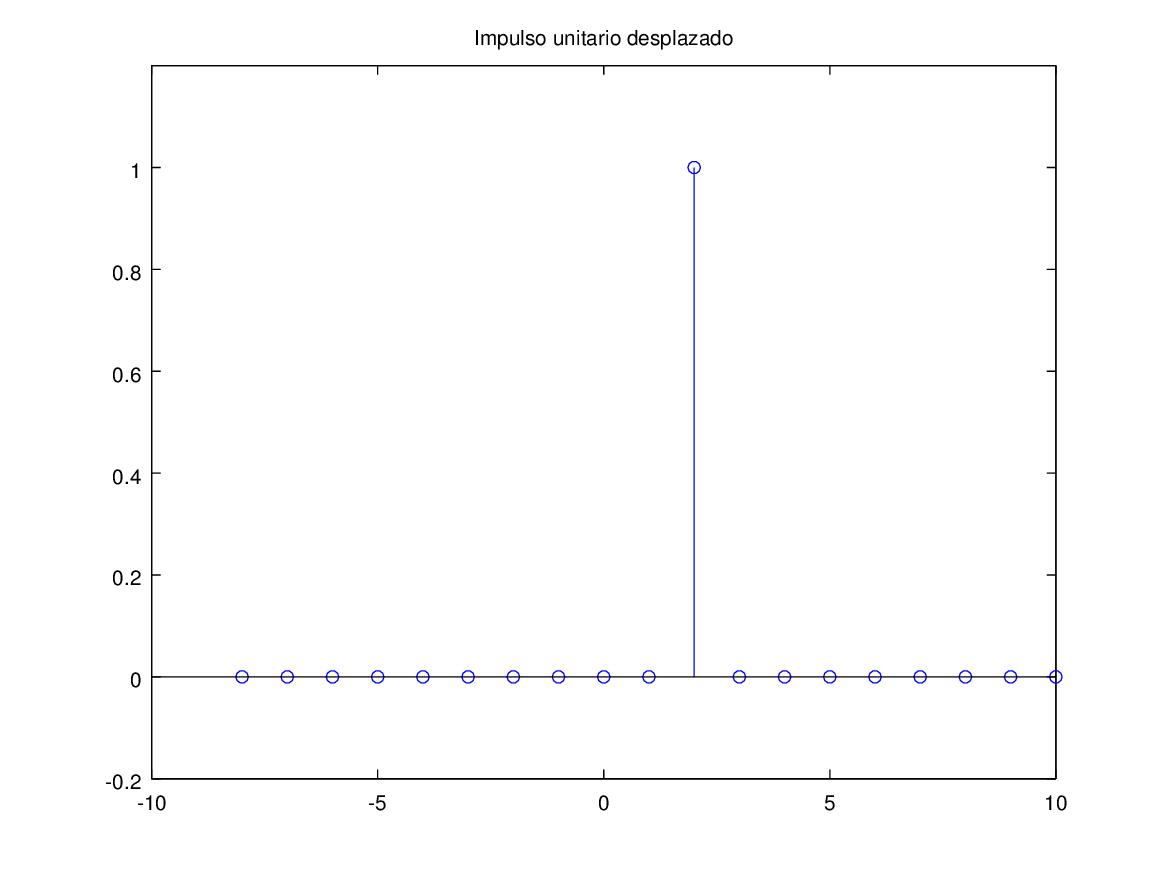
\includegraphics[height=3in]{./graphics/impunidiscdesp.eps}
  \caption{Impulso unitario de tiempo discreto desplazado.}
  \label{impunidiscdespeps}
\end{figure}

Tambi\'{e}n podemos multiplicar al impulso unitario por un valor real
$v$.  En este caso la definici\'{o}n es
\begin{equation}
  v \delta \left[ n - n_{0}\right] =\left\{ 
    \begin{array}{ll}
      0,      & n\neq n_{0}, \\ 
      v,      & n= n_{0}.
    \end{array}
  \right. 
\end{equation}
Vea la Fig. (\ref{impunidiscdespmulteps}).

\begin{figure}
  \centering
  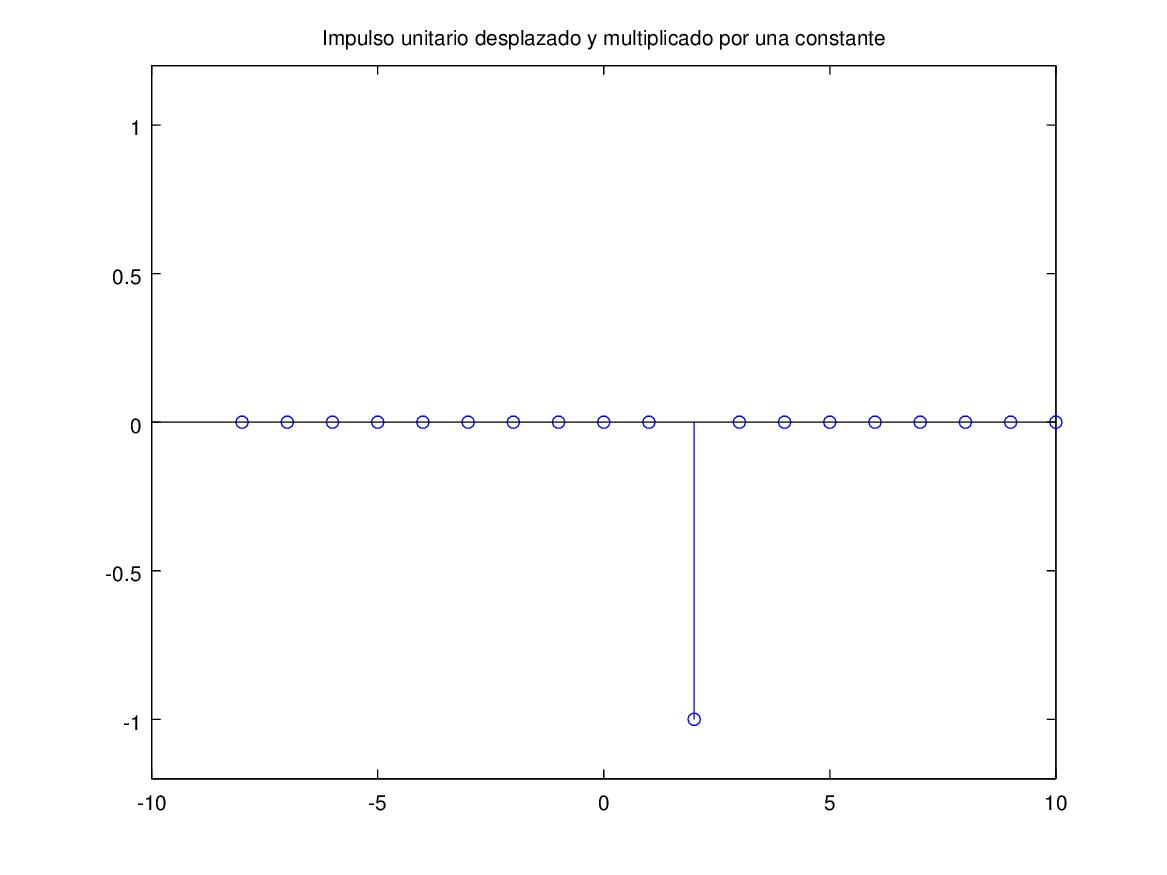
\includegraphics[height=3in]{./graphics/impunidiscdespmult.eps}
  \caption{Impulso unitario de tiempo discreto desplazado y
    multiplicado.}
  \label{impunidiscdespmulteps}
\end{figure}

\subsection{El escal\'{o}n unitario (tiempo discreto)}

Se define el escal\'{o}n unitario de tiempo discreto como
\begin{equation}
  u\left[ n\right] =\left\{ 
    \begin{array}{ll}
      0, & n<0, \\ 
      1, & n\geq 0.
    \end{array}
  \right.
\end{equation}
Vea la Fig. (\ref{escunidisceps}).

\begin{figure}
  \centering
  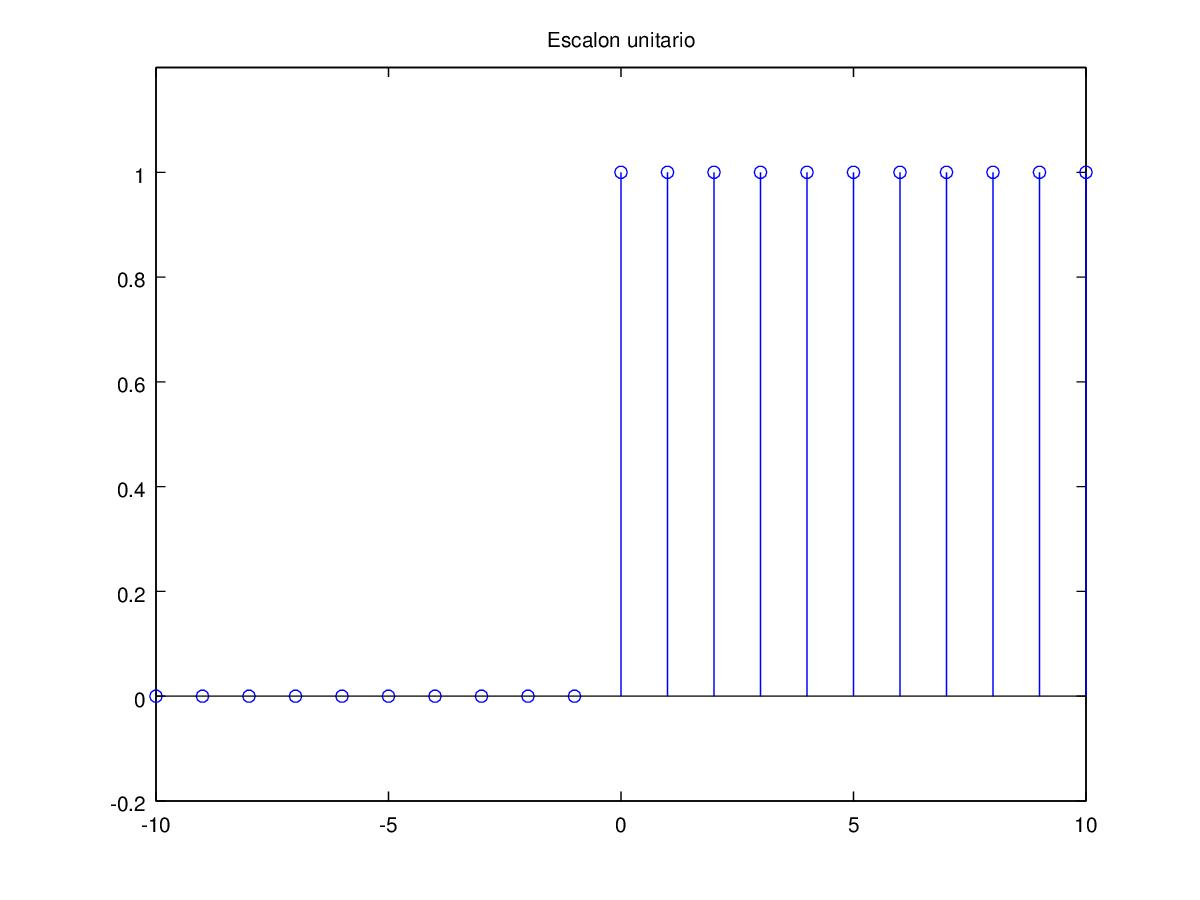
\includegraphics[height=3in]{./graphics/escunidisc.eps}
  \caption{Escal\'{o}n unitario de tiempo discreto.}
  \label{escunidisceps}
\end{figure}

Podemos desplazar al escal\'{o}n unitario en el tiempo. En este caso
la definici\'{o}n es
\begin{equation}
  u \left[ n - n_{0}\right] =\left\{ 
    \begin{array}{ll}
      0,      & n <    n_{0}, \\ 
      1,      & n \geq n_{0}.
    \end{array}
  \right.
\end{equation}
Vea la Fig. (\ref{escunidiscdespeps}).

\begin{figure}
  \centering
  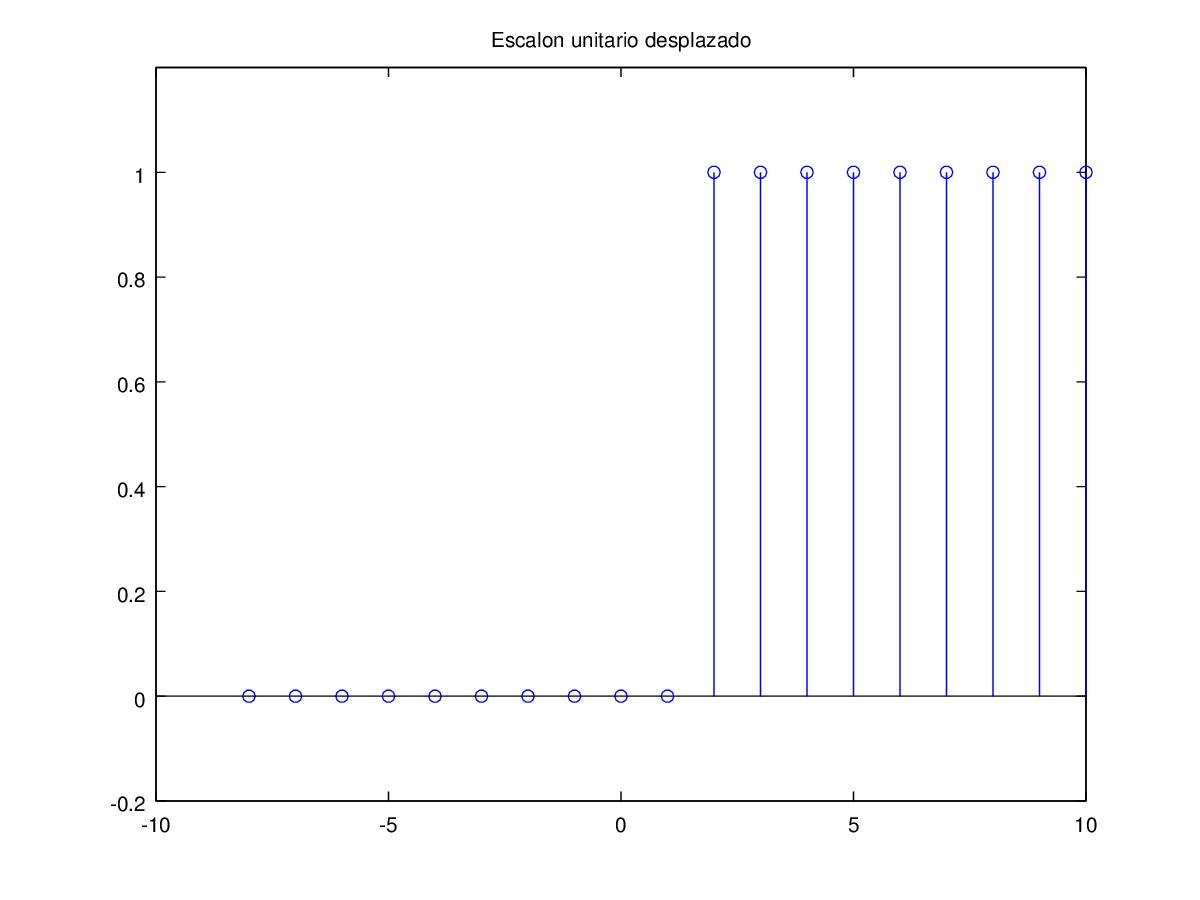
\includegraphics[height=3in]{./graphics/escunidiscdesp.eps}
  \caption{Escal\'{o}n unitario de tiempo discreto desplazado.}
  \label{escunidiscdespeps}
\end{figure}

Tambi\'{e}n podemos multiplicar al escal\'{o}n unitario por un valor
real $v$.  En este caso la definici\'{o}n es
\begin{equation}
  v u \left[ n - n_{0}\right] =\left\{ 
    \begin{array}{ll}
      0,      & n < n_{0}, \\ 
      v,      & n \geq n_{0}.
    \end{array}
  \right.
\end{equation}
Vea la Fig. (\ref{escunidiscdespmulteps}).

\begin{figure}
  \centering
  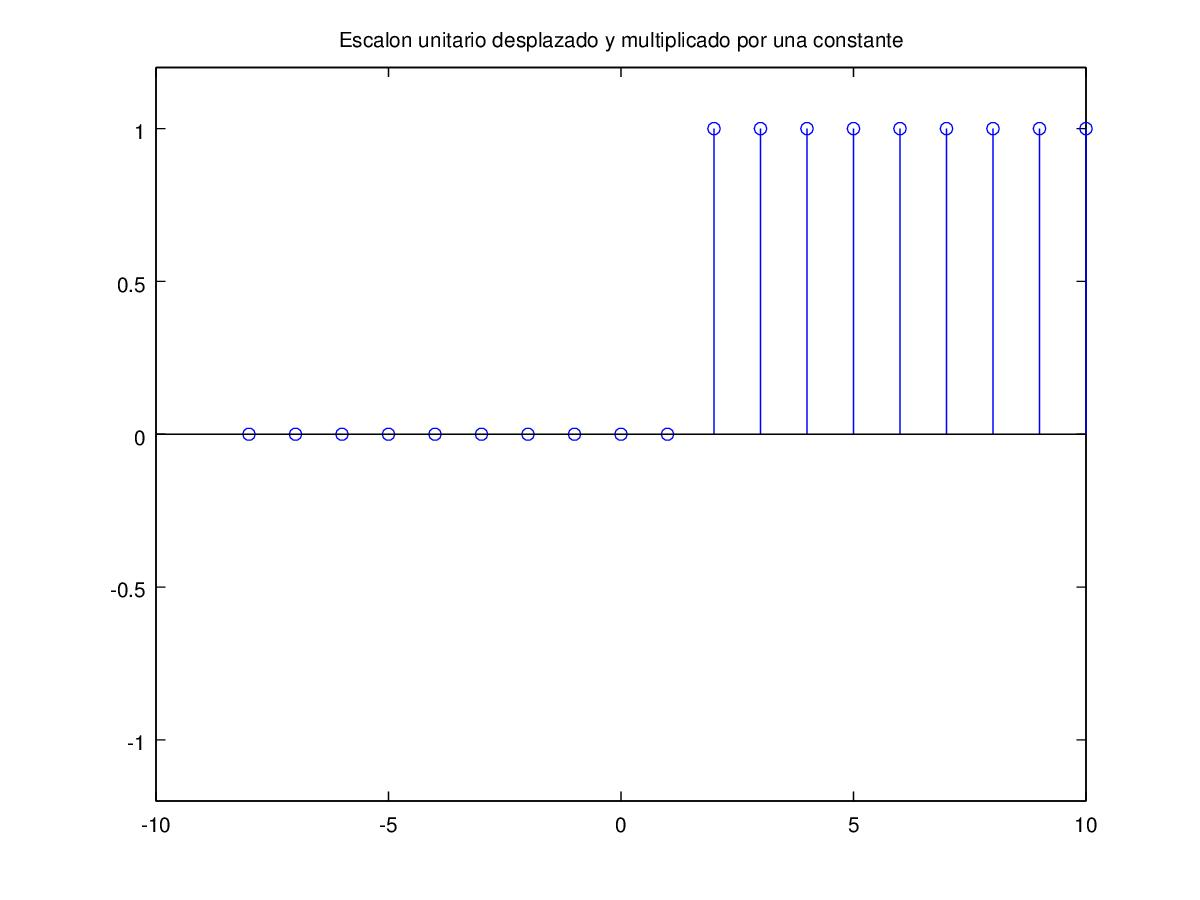
\includegraphics[height=3in]{./graphics/escunidiscdespmult.eps}
  \caption{Escal\'{o}n unitario de tiempo discreto desplazado y
    multiplicado.}
  \label{escunidiscdespmulteps}
\end{figure}

\subsection{Relaci\'{o}n entre impulso y escal\'{o}n (tiempo discreto)}

Las relaciones entre impulso y escal\'{o}n son las siguientes
\begin{eqnarray}
  \delta \left[ n\right] &=&u\left[ n\right] -u\left[ n-1\right] . \\
  u\left[ n\right] &=&\sum_{m=-\infty }^n\delta \left[ m\right] .
\end{eqnarray}
Cambiando $k=n-m$%
\begin{equation}
  u\left[ n\right] =\sum_{k=\infty }^{0}\delta \left[ n-k\right] ,
\end{equation}
o
\begin{equation}
  u\left[ n\right] =\sum_{k=0}^{\infty }\delta \left[ n-k\right] .
\end{equation}
Esta es la definici\'{o}n impl\'{i}cita del impulso, como la se\~{n}al
que sumada en el tiempo ``genera'' un escal\'{o}n. Vea la Fig.
(\ref{lecture02_text_gr10eps}).

Escribiendo
\begin{equation}
  u\left[ n\right] = 
\left(\sum_{k<n}^{\infty }\delta \left[n-k\right] \right) + 
\delta\left(0\right) + 
\left(\sum_{n<k}^{\infty }\delta \left[n-k\right] \right),
\end{equation}

\begin{figure}
  \centering
  \includegraphics[height=2in]{./graphics/lecture02_tex_gr10.eps}
  \caption{Impulso de tiempo discreto desplazado y
    multiplicado, y escalón unitario de tiempo discreto}
  \label{lecture02_text_gr10eps}
\end{figure}

\subsection{El escal\'{o}n unitario (tiempo continuo)}

Definimos el escal\'{o}n unitario de tiempo continuo como
\begin{equation}
  u\left( t\right) =\left\{ 
    \begin{array}{ll}
      0, & t < 0    \\ 
      1, & t > 0
    \end{array}
  \right.
\end{equation}
Observe que la funci\'{o}n tiene una discontinuidad en $t=0$.  Vea la
Fig. (\ref{lecture_text_gr9eps})


\subsection{El impulso unitario (tiempo continuo)}

Definimos el impulso unitario de tiempo continuo como
\begin{equation}
  u\left( t\right) =\int_{-\infty }^{t}\delta \left( \tau \right) d\tau . \label{escimpcont}
\end{equation}
Esta es la definici\'{o}n impl\'{i}cita del impulso, como la se\~{n}al
que integrada en el tiempo ``genera'' un escal\'{o}n.

\subsection{Construcci\'{o}n del impulso y el escal\'{o}n unitario}

La ecuaci\'{o}n (\ref{escimpcont}) nos da una definici\'{o}n de un
impulso pero no nos dice como construirlo. Para esto podemos ver al
impulso unitario como el l\'{\i}mite de una sucesi\'{o}n de funciones
de area unitaria.
\begin{enumerate}

\item Definamos una sucesi\'{o}n de funciones $r_{\Delta} \left( t -
    t_{0} \right) $ de \'{a}rea unitaria
  \begin{equation}
    r_{\Delta} \left( t - t_{0} \right) = \left \{
      \begin{array}{ll}
        0                       &       t < t_{0},                                              \\
        \frac{1}{\Delta}        &       t_{0}   \leq    t       \leq    t_{0} + \Delta,         \\
        0                       &       t_{0} + \Delta < t, 
      \end{array} 
    \right.
  \end{equation}
  donde $\Delta$ es una constante real no negativa. Vea la Fig.
  (\ref{sucimpconteps.1}). Esta no es la \'{u}nica forma de hacerlo, vea
  las Figs. (\ref{lecture02texgr7eps}) y (\ref{lecture02texgr8eps}).

\begin{figure}
  \centering
  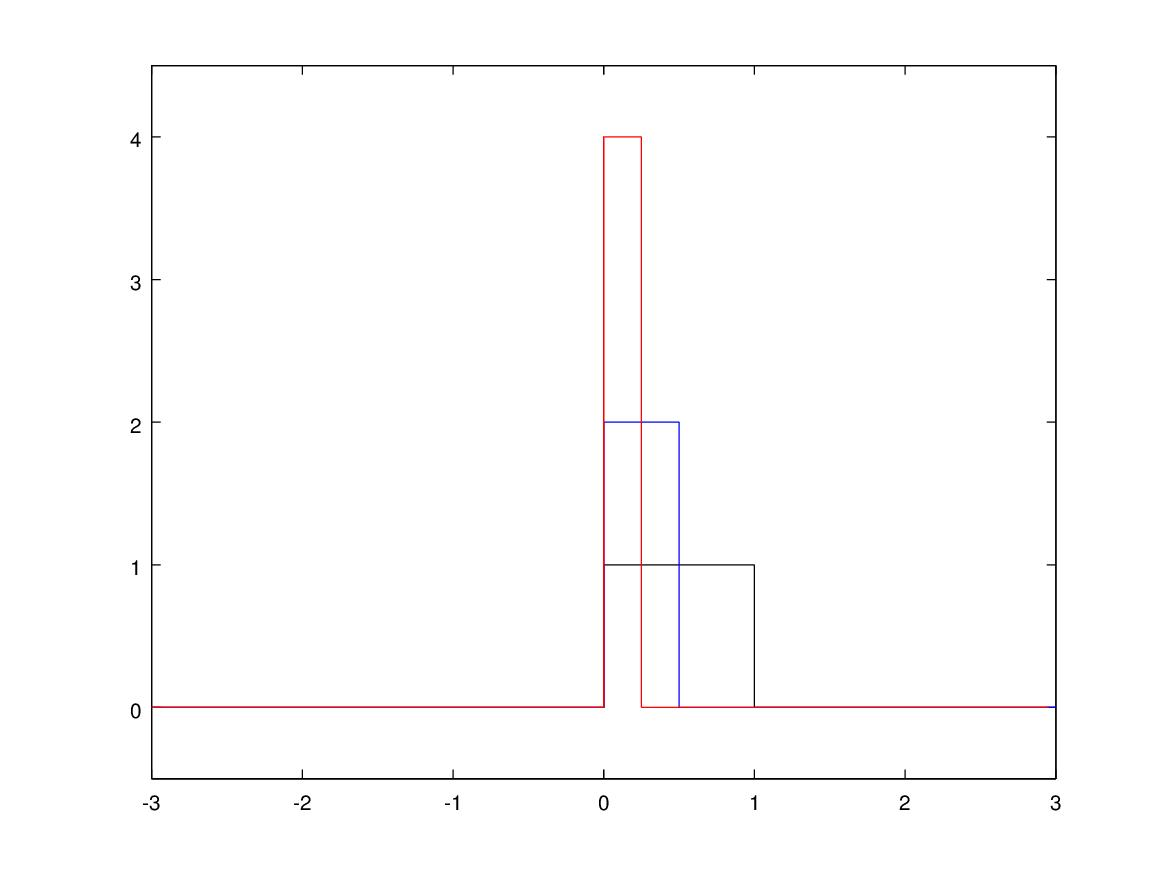
\includegraphics[height=3in]{./graphics/sucimpcont.eps}
  \caption{Sucesi\'{o}n de funciones que convergen a un impulso
    unitario de tiempo continuo.}
  \label{sucimpconteps.1}
\end{figure}

\begin{figure}
  \centering
  \includegraphics[height=3in]{./graphics/lecture02_tex_gr7.eps}
  \caption{Aproximaci\'{o}n del impulso unitario de tiempo continuo.}
  \label{lecture02texgr7eps}
\end{figure}

\begin{figure}
  \centering
  \includegraphics[height=3in]{./graphics/lecture02_tex_gr8.eps}
  \caption{Aproximaci\'{o}n del impulso unitario de tiempo continuo.}
  \label{lecture02texgr8eps}
\end{figure}

\item Tenemos entonces que el impulso $\delta \left( t \right)$ es el
  l\'{\i}mite
  \begin{equation}
    \delta \left( t - t_{0}\right) = 
    \begin{array}{l}
      Lim                             \\
      \Delta \rightarrow 0
    \end{array}
    r_{\Delta} \left( t - t_{0} \right).            \label{impunsuc}
  \end{equation}

\item Definamos tambi\'{e}n una sucesi\'{o}n de funciones $s_{\Delta}
  \left( t \right)$ dadas por
  \begin{equation}
    s_{\Delta} \left( t - t_{0} \right) = \left \{
      \begin{array}{ll}
        0,                      &       t < t_{0},                              \\
        \frac{t}{\Delta},       &       t_{0} \leq t \leq t_{0} + \Delta,       \\
        1,                      &       t_{0} + \Delta < t.
      \end{array}
    \right.         \label{escunsuc}
  \end{equation}
  Vea la Fig. (\ref{sucescconteps}).

\begin{figure}
  \centering
  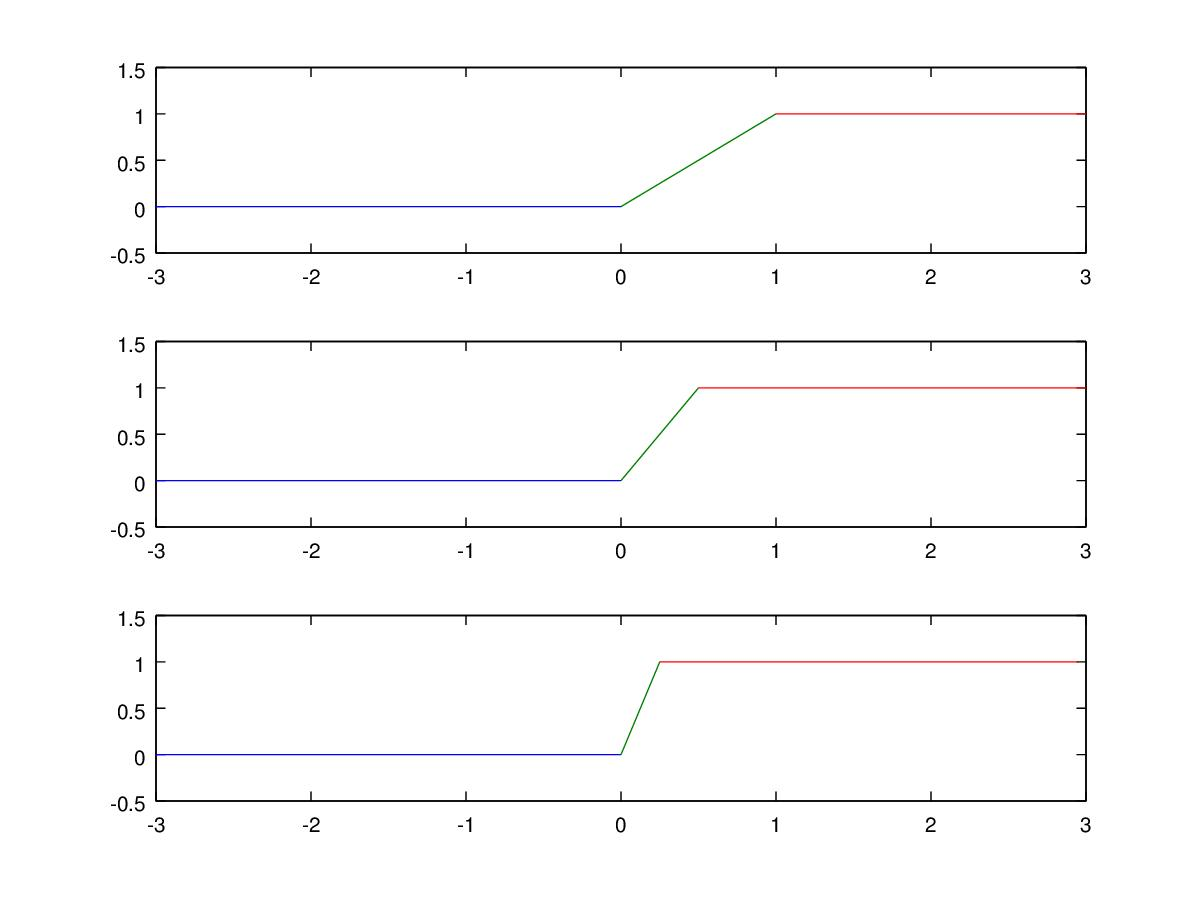
\includegraphics[height=3in]{./graphics/sucesccont.eps}
  \caption{Sucesi\'{o}n de funciones que convergen a un escal\'{o}n
    unitario de tiempo continuo.}
  \label{sucescconteps}
\end{figure}
        
\item Tenemos entonces que el escal\'{o}n $u \left( t \right)$ es el
  l\'{\i}mite
  \begin{equation}
    u \left( t - t_{0} \right) = 
    \begin{array}{l}
      Lim                             \\
      \Delta \rightarrow 0
    \end{array}
    s_{\Delta} \left( t - t_{0} \right).
  \end{equation}
  Vea la Fig. (\ref{lecture_text_gr9eps}).

  % \begin{figure}
  %   \centering
  %   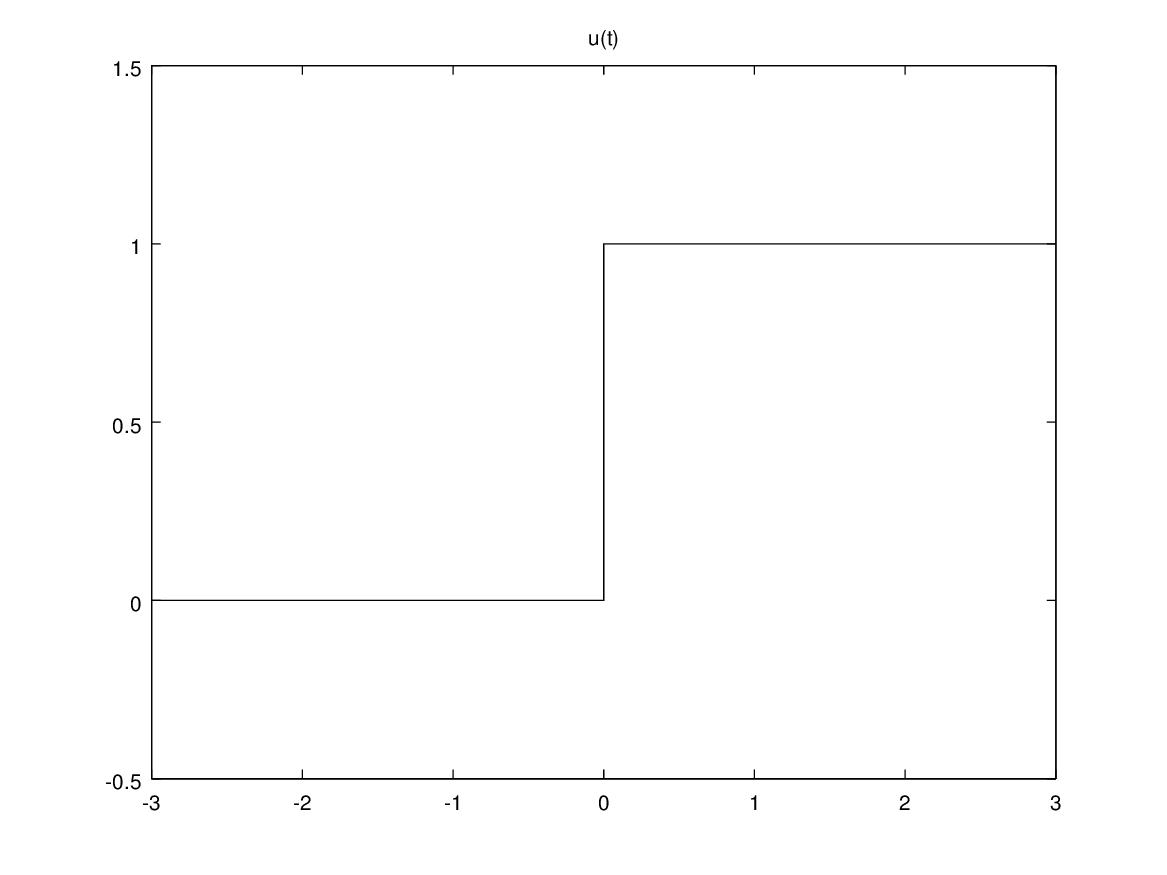
\includegraphics[height=3in]{./graphics/limesccont.eps}
  %   \caption{L\'{\i}mite de una sucesi\'{o}n de funciones que
  %     convergen a un escal\'{o}n unitario de tiempo continuo.}
  %   \label{limescconteps}
  % \end{figure}

\begin{figure}
  \centering
  \includegraphics[height=3in]{./graphics/lecture02_tex_gr9.eps}
  \caption{Escal\'{o}n unitario de tiempo continuo}
  \label{lecture_text_gr9eps}
\end{figure}
        
\end{enumerate}

\subsubsection{Impulso en el tiempo}

\begin{enumerate}
\item Un impulso de corriente en tiempo entrega una unidad de carga
  instan-t\'{a}neamente a un circuito.

\item Un impulso de fuerza en tiempo entrega un momento
  instant\'{a}neo a un mecanismo.
\end{enumerate}

\subsubsection{Impulso en el espacio}

\begin{enumerate}

\item Un impulso de masa en el espacio es una masa puntual.

\item Un impulso de densidad de carga en el espacio es una carga
  puntual.

\item Un impulso de intensidad de luz en el espacio es una luz
  puntual.
\end{enumerate}

% \subsection{Ejercicios para hacer}
% 
% Escriba las definiciones de las se\~{n}ales singulares expuestas en esta secci\'{o}n.
% 
% De ejemplos gr\'{a}ficos en Matlab.
% 
\section{Se\~{n}ales muestreadas}

El muestreo de se\~{n}ales es una operaci\'{o}n muy importante. Preste
atenci\'{o}n.  Veremos primero el muestreo en tiempo discreto, y despu\'{e}s en tiempo continuo.

\subsection{Tiempo discreto}

\begin{enumerate}
\item Recordemos la definici\'{o}n del impulso unitario de tiempo
  discreto
  \begin{equation}
    \delta \left[ n - n_{0}\right] =\left\{ 
      \begin{array}{ll}
        0, & n\neq n_{0}, \\ 
        1, & n = n_{0}.
      \end{array}
    \right.
  \end{equation}

\item Supongamos que tenemos una se\~{n}al $x[n]$. Podemos obtener una
  nueva se\~{n}al
  \begin{equation}
    z[n] = x[n] \delta[n - n_{0}],
  \end{equation}
  de la siguiente forma
  \begin{equation}
    z[n] = \left \{
      \begin{array}{ll}
        0       &       n \neq n_{0},   \\
        x[n_{0}]        & n  = n_{0}.
      \end{array}             \label{muesdiscre}
    \right.
  \end{equation}

\item Podemos resumir la operaci\'{o}n realizada en la ec.
  (\ref{muesdiscre}) como
  \begin{equation}
    x\left[ n\right] \delta \left[ n-n_{0}\right] =
    x\left[ n_{0}\right] \delta \left[ n-n_{0}\right], \label{claveuno}
  \end{equation}
  y la denominaremos muestreo en tiempo discreto.

\item La ec. (\ref{claveuno}) es una de las claves de esta materia.
  Por favor recuerdela.
\end{enumerate}

\subsection{Tiempo continuo}

\begin{enumerate}
\item Recordemos la definici\'{o}n \textbf{de la sucesi\'{o}n de
    funciones} cuyo l\'{\i}mite es el impulso unitario
  \begin{equation}
    r_{\Delta} \left( t - t_{0} \right) = \left \{
      \begin{array}{ll}
        0                       &       t < t_{0},                                              \\
        \frac{1}{\Delta}        &       t_{0} \leq      t       \leq    t_{0} + \Delta,         \\
        0                       &       t_{0} + \Delta < t ,
      \end{array} 
    \right.
  \end{equation}
  donde $\Delta$ es una constante real no negativa.

\item Supongamos que tenemos una se\~{n}al $x \left( t \right)$.
  Podemos obtener una nueva se\~{n}al
  \begin{equation}
    z \left( t \right) = x \left( t \right) \delta \left( t - t_{0}\right),
  \end{equation}
  de la siguiente forma
  \begin{enumerate}
  \item Construyamos una sucesi\'{o}n de funciones
    \begin{equation}
      z_{\Delta} \left( t \right) = \left \{
        \begin{array}{ll}
          0                                       &       t < t_{0},                              \\
          x\left( t_{0} \right) \frac{1}{\Delta}      &       t_{0} \leq t \leq t_{0} + \Delta,       \\
          0                                       &       t_{0} + \Delta < t,
        \end{array} 
      \right.
    \end{equation}
                        
  \item La funci\'{o}n $z \left( t \right)$ es el l\'{\i}mite de la
    sucesi\'{o}n cuando $\Delta \rightarrow 0$.
                        
  \end{enumerate}
  \begin{equation}
    z \left( t \right) = 
    x\left( t\right) \delta \left( t-t_{0}\right) =
    x\left( t_{0}\right) \delta \left(
      t-t_{0}\right) . \label{clavedos}
  \end{equation}

\item La ec. (\ref{clavedos}) es una de las claves de esta materia.
  Por favor recuerdela.
\end{enumerate}

% \subsection{Ejercicios para hacer}

% Escriba su propia versi\'{o}n de esta secci\'{o}n, con ejemplos gr\'{a}ficos en Matlab incluidos.

\section{Energ\'{\i}a y potencia}

A continuaci\'{o}n analizamos dos importantes propiedades de las
se\~{n}ales en general. La energ\'{\i}a y potencia de una se\~{n}al
son funciones que dependen de un lapso determinado de tiempo.

Consideremos el caso especial de un circuito el\'{e}ctrico con una
resistencia $R$ sujeta a una diferencia de potencial $v(t)$ y una
corriente $i(t) = \frac{v(t)}{R}$. La potencia instant\'{a}nea por ohm
est\'{a} definida como
\begin{equation}
  p(t) = v(t) \, i(t) = \frac{i^{2}(t)}{R}.
\end{equation}
La energ\'{\i}a total $E$ se define como
\begin{equation}
  E = 
  \begin{array}{l}
    Lim \\ 
    T\rightarrow \infty
  \end{array}
\int_{-T}^{T} i^{2}(t) dt,
\end{equation}
y la potencia promedio $P$ por ohm se define como
\begin{equation}
  P =         
  \begin{array}{l}
    Lim \\ 
    T\rightarrow \infty
  \end{array}
  \frac{1}{2 \, T} \int_{-T}^{T} i^{2}(t) dt.
\end{equation}

\subsection{Energ\'{\i}a de una se\~{n}al de tiempo continuo}

La energ\'{\i}a en un lapso determinado de tiempo se define como
\begin{equation}
  E_{t_{2},t_{1}}=\int_{t_{1}}^{t_{2}}\left| x\left( t\right) \right| ^{2}dt.
\end{equation}
La energ\'{\i}a total de una se\~{n}al se define como
\begin{equation}
  E_{\infty }= 
  \begin{array}{l}
    Lim \\ 
    T\rightarrow \infty
  \end{array}
  \int_{-T}^{T}\left| x\left( t\right) \right| ^{2}dt.
\end{equation}

\subsection{Energ\'{\i}a de una se\~{n}al de tiempo discreto}

La energ\'{\i}a en un lapso determinado de tiempo se define como
\begin{equation}
  E_{n_{2},n_{1}}=\sum_{n=n_{1}}^{n_{2}}\left| x\left[ n\right] \right| ^{2}.
\end{equation}
La energ\'{\i}a total de una se\~{n}al se define como
\begin{equation}
  E_{\infty }= 
  \begin{array}{l}
    Lim \\ 
    N\rightarrow \infty
  \end{array}
  \sum_{n=-N}^{N}\left| x\left[ n\right] \right| ^{2}.
\end{equation}

\subsection{Potencia de una se\~{n}al de tiempo continuo}

La potencia en un lapso determinado de tiempo se define como
\begin{equation}
  P_{t_{2},t_{1}}=\frac{1}{t_{2}-t_{1}}\int_{t_{1}}^{t_{2}}\left| x\left(t\right) \right| ^{2}dt.
\end{equation}
La potencia total de una se\~{n}al se define como
\begin{equation}
  P_{\infty }= 
  \begin{array}{l}
    Lim \\ 
    T\rightarrow \infty
  \end{array}
  \frac{1}{2T}\int_{-T}^{T}\left| x\left( t\right) \right| ^{2}dt.
\end{equation}

\subsection{Potencia de una se\~{n}al de tiempo discreto}

La potencia de una se\~{n}al de tiempo discreto en un lapso
determinado de tiempo se define como
\begin{equation}
  P_{n_{2},n_{1}}=\frac{1}{n_{2}-n_{1}+1}\sum_{n=n_{1}}^{n_{2}}\left| x\left[ n\right] \right| ^{2}.
\end{equation}
La potencia total de una se\~{n}al de tiempo discreto se define como
\begin{equation}
  P_{\infty }= 
  \begin{array}{l}
    Lim \\ 
    N\rightarrow \infty
  \end{array}
  \frac{1}{2N+1}\sum_{n=-N}^{N}\left| x\left[ n\right] \right| ^{2}.
\end{equation}

\subsection{Se\~{n}al de energ\'{\i}a}

La se\~{n}al $x$ es de energ\'{\i}a finita (o se\~{n}al $x$ de
energ\'{\i}a) si y s\'{o}lo si $0 < E < \infty$, lo que implica $P =
0$.

\subsection{Se\~{n}al de potencia}

La se\~{n}al $x$ es de potencia finita (o se\~{n}al $x$ de potencia)
si y s\'{o}lo si $0 < P < \infty$, lo que implica $E = \infty$.

\subsection{Decibeles}

\subsubsection{Definici\'{o}n}

El decibel o $dB$ es la d\'{e}cima parte de un bel, una unidad de
medida relativa. Supongamos que deseamos expresar en Bels la potencia
medida $P_{m}$, con respecto a la potencia de referencia. Tenemos
entonces la relaci\'{o}n
\begin{equation}
  A_{B} = log_{10}(\frac{P_{m}}{P_{r}}).
\end{equation}
En otras palabras, $A_{B}$, la potencia medida $P_{m}$ expresada en Bels, es 
igual al logaritmo en base 10 de la potencia
$P_{m}$ relativa a una potencia de referencia $P_{r}$.  La
elecci\'{o}n de la potencia de referencia define la escala usada.

Dado que la potencia est\'{a} calculada en base a la norma
cuadrática de la se\~{n}al, podemos escribir
\begin{equation}
  A_{B} = 2 \, log_{10}(\frac{|A_{m}|}{|A_{r}|}),
\end{equation}
donde $A_{m}$ y $A_{r}$ son las amplitudes de las se\~{n}ales medida y
de referencia.  Adem\'{a}s como hay 10 decibeles en un bel, tenemos
\begin{equation}
  A_{dB} = 20 \, log_{10}(\frac{|A_{m}|}{|A_{r}|}),
\end{equation}

\subsubsection{Décadas y octavas}


Veamos la figura \ref{decoctpng} para entender como definir
décadas y octavas en escalas logarítmicas de medida. Tanto décadas como octavas son unidades de medida para escalas logarítmicas. Observemos que necesitamos una referencia $X$ para después poder
marcar la década $10 \, X$ y la octava $2 \, X$.

\begin{figure}
	\centering
	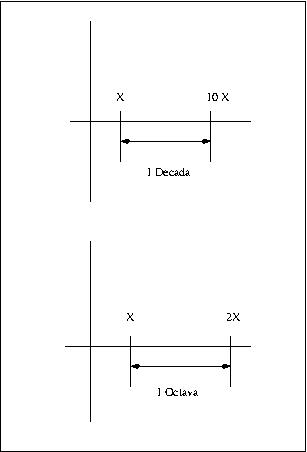
\includegraphics[height=6in, width=4in]{./graphics/decoct.png}
	\caption{D\'{e}cadas y octavas}
	\label{decoctpng}
\end{figure}


\subsubsection{Propiedades de las escalas en dB}

En todas las clases de dB, un factor de $10$ en la amplitud de la
se\~{n}al medida corresponde a un incremento de $20$ decibeles
\begin{equation}
  20 \, log_{10}(\frac{10 |A_{m}|}{|A_{r}|}) = 20 \, log_{10}(10) + 20 \, log_{10}(\frac{|A_{m}|}{|A_{r}|}).
\end{equation}

Una funci\'{o}n $f(x)$ que es proporcional a $\frac{1}{x}$ se dice que
``cae'' o disminuye a una raz\'{o}n de $20 dB$ por d\'{e}cada. Esto es, por cada
factor de $10$ en $x$ (cada d\'{e}cada), la amplitud cae $20 dB$.

En forma similar, un factor de $2$ en la amplitud corresponde a una
variaci\'{o}n de (aproximadamente) $6 dB$:
\begin{equation}
  20 \, log_{10} (\frac{2 |A_{m}|}{|A_{r}|}) = 20 \, log_{10}(2) + 20 \, log_{10}(\frac{|A_{m}|}{|A_{r}|}).
\end{equation}
Una funci\'{o}n que es proporcional a $\frac{1}{x}$ se dice que cae $6
dB$ por octava, o sea que por cada factor de $2$ en $x$ (por cada
octava) la amplitud disminuye aproximadamente $6 dB$. Entonces $6 dB$
por octava equivale a $20 dB$ por d\'{e}cada.

Finalmente, observemos que la elecci\'{o}n de la referencia determina
el desplazamiento vertical en la escala de $dB$:
\begin{equation}
  20 \, log_{10}(\frac{|A_{m}|}{|A_{r}|}) = 20 \, log_{10} (|A_{m}|) - 20 \, log_{10} (|A_{r}|),
\end{equation}
donde $-20 \, log_{10} (|A_{r}|)$ es el desplazamiento constante de la
escala vertical.

\subsubsection{Escalas en dB}

Dado que frecuentemente cambiamos las escalas de nuestras se\~{n}ales
para acomodarlas a nuestras necesidades parece ser in\'{u}til en
preocuparse por cu\'{a}l es la referencia de la escala en $dB$.  Sin
embargo, hay algunas escalas que debemos conocer.

\paragraph{Escala dBm} 
La referencia de potencia es $1 mW$ disipado en un
resistor de $600 \Omega$.

\paragraph{Escala dBV} 
La referencia de amplitud es $1$ volt. Entonces una se\~{n}al de $100$
volts equivale a
\begin{equation}
  20 log_{10} (\frac{100}{1}) = 40 dBV.
\end{equation}

\paragraph{Escala dB SPL} 
La referencia es la amplitud de una sinusoide de $1000$ hz de
frecuencia que ejerce una presi\'{o}n de $20 \, mBar = 20 \, \mu Pa$.
En unidades de intensidad sonora la referencia es igual a
\begin{equation}
  I_{0} = 10^{-16} \frac{W}{cm^{2}}.
\end{equation}
Dado que el sonido se crea mediante una presi\'{o}n variante en el
tiempo, calculamos niveles de sonido en $dB \, SPL$ usando la intensidad
promedio (calculada a lo largo de por lo menos un per\'{\i}odo de la
menor frecuencia contenida en el sonido).

\begin{tabular}{ll}
  Sonido                                          &       dB SPL  \\
  Motor jet a tres metros                         &       140     \\
  Umbral de dolor                                 &       130     \\
  Concierto de Rock                               &       120     \\
  Moto acelerando a cinco metros                  &       110     \\
  Martillo neum\'{a}tico a dos metros             &       100     \\
  F\'{a}brica                                     &       90      \\
  Aspiradora                                      &       80      \\
  Tr\'{a}fico pesado                              &       70      \\
  Restaurante quieto                              &       50      \\
  Area residencial a la noche                     &       40      \\
  Cine vacio                                      &       30      \\
  Murmullo de hojas secas                         &       20      \\
  Respiraci\'{o}n de una persona a tres metros    &       10      \\
  Umbral de audici\'{o}n                          &       0       
\end{tabular}

\paragraph{Escala dB para gr\'{a}ficos} 
La referencia elegida es la m\'{a}xima amplitud de la se\~{n}al:  Normalizamos la se\~{n}al tomando la m\'{a}xima amplitud como referencia,
a la que le corresponderá una medida en decibeles de $0 dB$. 
Para poder realizar esta normalizaci\'{o}n es evidente que necesitamos
conocer la se\~{n}al en un lapso de tiempo. Despu\'{e}s de encontrar
el m\'{a}ximo en dicho intervalo reci\'{e}n podemos realizar los
c\'{a}lculos.

\subsection{Ejemplo: Energ\'{\i}a promedio para la exponencial imaginaria de tiempo continuo en un período $T_{0}$}

Calculemos la energ\'{\i}a promedio de la exponencial imaginaria
en su per\'{\i}odo
\begin{equation}
  E_{T_{0}}=\int_{0}^{T_{0}}\left| e^{j \, \omega_{0} \, t}\right|
  ^{2}dt=\int_{0}^{T_{0}}\left( \cos \left( \omega_{0} \, t\right) ^{2}+\sin
    \left( \omega_{0} \, t\right) ^{2}\right) dt=T_{0}. \label{potfmuno}
\end{equation}

\subsection{Ejemplo: Potencia promedio para la exponencial imaginaria de tiempo continuo en un período $T_{0}$}

Calculemos su potencia promedio en un per\'{\i}odo $T_{0}$ 
\begin{equation}
  P_{T_{0}}=\frac{1}{T_{0}}E_{T_{0}}=\frac{1}{T_{0}}T_{0}=1. \label{potfmdos}
\end{equation}

\subsection{Ejemplo: Potencia promedio para la exponencial imaginaria de tiempo continuo en lapso de tiempo infinito}

Calculemos ahora su potencia promedio
\begin{equation}
  P_{\infty }= 
  \begin{array}{l}
    Lim \\ 
    T_{0}\rightarrow \infty
  \end{array}
  \frac{1}{2T_{0}}\int_{-T_{0}}^{T_{0}}\left| e^{j \, \omega_{0} \, t}\right|^{2}dt.
\end{equation}
\begin{equation}
  P_{\infty }= 
  \begin{array}{l}
    Lim \\ 
    T_{0}\rightarrow \infty
  \end{array}
  \frac{2T_{0}}{2T_{0}}=1.
\end{equation}

\subsection{Ejemplo: Energ\'{\i}a y potencia para señales de tiempo discreto}

\begin{enumerate}

\item Calculemos los valores de $E_{\infty }$ y $P_{\infty }$ para 
el escal\'{o}n $x_{1}\left[ n\right] =u[n]$.
Planteamos la f\'{o}rmula de energ\'{\i}a
  \begin{equation}
    E_{\infty }\left( x_{1}\left[ n\right] \right) = 
    \begin{array}{c}
      Lim \\ 
      N\rightarrow \infty
    \end{array}
    \sum_{n=-N}^{N}\left( u\left[ n\right] \right) ^{2},
  \end{equation}
Considerando que el escal\'{o}n es nulo ($u[n] = 0$) para $n$ negativo
$n < 0$, cambiamos el l\'{\i}mite inferior de la sumatoria a $0$. Dado
que el escal\'{o}n es igual a $1$ para $n$ no negativo ($n \geq 0$), reemplazamos $u(n)$
por $1$. Entonces resolvemos 
  \begin{equation}
    E_{\infty }\left( x_{1}\left[ n\right] \right) = 
    \begin{array}{c}
      Lim \\ 
      N\rightarrow \infty
    \end{array}
    \sum_{n=0}^{N} 1 =\infty.
  \end{equation}
Planteamos la f\'{o}rmula de potencia
  \begin{equation}
    P_{\infty }\left( x_{1}\left[ n\right] \right) = 
    \begin{array}{c}
      Lim \\ 
      N\rightarrow \infty
    \end{array}
    \frac{\sum_{n=-N}^{N}\left( u\left[ n\right] \right) ^{2}}{2N+1},
  \end{equation}
y con las mismas consideraciones que para el c\'{a}lculo de la
energ\'{i}a resolvemos
  \begin{equation}
    P_{\infty }\left( x_{1}\left[ n\right] \right) = 
    \begin{array}{c}
      Lim \\ 
      N\rightarrow \infty
    \end{array}
    \frac{\sum_{n=0}^{N}1}{2N+1}=\frac{1}{2}.
  \end{equation}

\item Calculemos los valores de $E_{\infty }$ y $P_{\infty }$ para 
$x_{2}[n]=2^{-n}u\left[ n\right].$
Planteamos la f\'{o}rmula de energ\'{\i}a
  \begin{equation}
    E_{\infty }\left( x_{2}\left[ n\right] \right) = 
    \begin{array}{c}
      Lim \\ 
      N\rightarrow \infty
    \end{array}
    \sum_{n=-N}^{N}\left( 2^{-n}u\left[ n\right] \right) ^{2}.
  \end{equation}
Considerando que el escal\'{o}n es nulo ($u[n] = 0$) para $n$ negativo
($n < 0$), cambiamos el l\'{\i}mite inferior a $n = 0$. Dado que el escal\'{o}n
es igual a $1$ ($u[n] = 1$) para $n$ no negativo ($n \geq 0$), reemplazamos $u[n]$ por $1$.
Resolvemos
  \begin{equation}
    E_{\infty }\left( x_{2}\left[ n\right] \right)= 
    \begin{array}{c}
      Lim \\ 
      N\rightarrow \infty
    \end{array}
    \sum_{n=0}^{N}\left( 4^{-n}\right) =\frac{1}{1-\frac{1}{4}}=\frac{4}{3},
  \end{equation}
aplicando la propiedad de las sumas geom\'{e}tricas
\begin{equation}
  \sum_{n = 0}^{N} q^{n} = \frac{1-q^{N+1}}{1-q},
\end{equation}
y su l\'{\i}mite
\begin{equation}
  \begin{array}{c}
    Lim \\
    n \rightarrow \infty
  \end{array}
  \frac{1-q^{n+1}}{1-q} =   \frac{1}{1-q},
\end{equation}
para $\parallel q \parallel_{2} < 1$.
Planteamos la f\'{o}rmula de potencia
  \begin{equation}
    P_{\infty }\left( x_{2}\left[ n\right] \right) = 
    \begin{array}{c}
      Lim \\ 
      N\rightarrow \infty
    \end{array}
    \frac{\sum_{n=-N}^{N}\left( 2^{-n}u\left[ n\right] \right) ^{2}}{2N+1},
  \end{equation}
y con las mismas consideraciones que para el c\'{a}lculo de la
energ\'{i}a resolvemos
  \begin{equation}
    P_{\infty }\left( x_{2}\left[ n\right] \right) = 
    \begin{array}{c}
      Lim \\ 
      N\rightarrow \infty
    \end{array}
    \frac{\frac{4}{3}}{2N+1}=0.
  \end{equation}

\item Calculamos los valores de $E_{\infty }$ y $P_{\infty }$ para 
$x_{3}\left[ n\right] =u\left[ n\right] -u\left[ n-2\right]$.
Planteamos la f\'{o}rmula de energ\'{\i}a
\begin{equation}
E_{\infty }\left( x_{3}\left[ n\right] \right) = 
\begin{array}{c}
Lim \\ 
N\rightarrow \infty
\end{array}
\sum_{n=-N}^{N}\left( u\left[ n\right] -u\left[ n-2\right] \right) ^{2}.
\end{equation}
Observemos que la funci\'{o}n es igual a $1$ para $0 \leq n < 2$, e
igual a $0$ para $n < 0$ y $n \leq 2$.Por lo tanto los l\'{\i}mites
de la sumatoria pueden cambiarse a $n = 0$ y $n = 2$.
Podemos resolver
\begin{equation}
E_{\infty }\left( x_{3}\left[ n\right] \right) = 
\begin{array}{c}
Lim \\ 
N\rightarrow \infty
\end{array}
2=2.
\end{equation}
Planteamos la f\'{o}rmula de potencia
\begin{equation}
P_{\infty }\left( x_{3}\left[ n\right] \right) = 
\begin{array}{c}
Lim \\ 
N\rightarrow \infty
\end{array}
\frac{\sum_{n=-N}^{N}\left( u\left[ n\right] -u\left[ n-2\right] \right)
^{2}}{2N+1},
\end{equation}
y resolvemos
\begin{equation}
P_{\infty }\left( x_{3}\left[ n\right] \right) = 
\begin{array}{c}
Lim \\ 
N\rightarrow \infty
\end{array}
\frac{2}{2N+1}=0.
\end{equation}

\item Calculamos los valores de $E_{\infty }$ y $P_{\infty }$ para 
$x_{4}\left[ n\right] =
  \cos \left( \frac{\pi }{4}n\right) \left( u\left[ n\right] -u\left[
      n-4\right] \right)$.
Planteamos la f\'{o}rmula de energ\'{\i}a
\begin{equation}
E_{\infty }\left( x_{4}\left[ n\right] \right) = 
\begin{array}{c}
Lim \\ 
N\rightarrow \infty
\end{array}
\sum_{n=-N}^{N}\left( \cos \left( \frac{\pi }{4}n\right) \left( u\left[ n
\right] -u\left[ n-4\right] \right) \right) ^{2},
\end{equation}
y resolvemos
\begin{equation}
E_{\infty }\left( x_{4}\left[ n\right] \right) = 
\begin{array}{c}
Lim \\ 
N\rightarrow \infty
\end{array}
2=2,
\end{equation}
Planteamos la f\'{o}rmula de potencia
\begin{equation}
P_{\infty }\left( x_{4}\left[ n\right] \right) = 
\begin{array}{c}
Lim \\ 
N\rightarrow \infty
\end{array}
\frac{\sum_{n=-N}^{N}\left( \cos \left( \frac{\pi }{4}n\right) \left(
      u\left[ n\right] -u\left[ n-4\right] \right) \right)
  ^{2}}{2N+1}.
\end{equation}
y resolvemos
\begin{equation}
P_{\infty }\left( x_{4}\left[ n\right] \right) = 
\begin{array}{c}
Lim \\ 
N\rightarrow \infty
\end{array}
\frac{2}{2N+1}=0.
\end{equation}

\item Calculamos los valores de $E_{\infty }$ y $P_{\infty }$ para 
$x_{5}\left( t\right) =\cos \left( t\right)$.
Planteamos la f\'{o}rmula de energ\'{\i}a y resolvemos
\begin{equation}
E_{\infty }\left( x_{5}\left( t\right) \right) = 
\begin{array}{c}
Lim \\ 
T\rightarrow \infty
\end{array}
\int_{-T}^{T}\left( \cos \left( t\right) \right) ^{2}dt = \infty.
\end{equation}
Planteamos la f\'{o}rmula de potencia
\begin{equation}
P_{\infty }\left( x_{5}\left( t\right) \right) = 
\begin{array}{c}
Lim \\ 
T\rightarrow \infty
\end{array}
\frac{\int_{-T}^{T}\left( \cos \left( t\right) \right) ^{2}dt}{2T}= 
\begin{array}{c}
Lim \\ 
T\rightarrow \infty
\end{array}
\frac{T+\frac{1}{2}\sin \left( 2T\right) }{2T},
\end{equation}
y resolvemos
\begin{equation}
P_{\infty }\left( x_{5}\left( t\right) \right) = 
\begin{array}{c}
Lim \\ 
T\rightarrow \infty
\end{array}
\frac{T+\frac{1}{2}\sin \left( 2T\right) }{2T}=\frac{1}{2}.
\end{equation}

\item Calculamos los valores de $E_{\infty }$ y $P_{\infty }$ para 
$x_{6}\left( t\right) =e^{j\left( 2t+\frac{\pi }{4}\right) }$.
Planteamos la f\'{o}rmula de energ\'{\i}a
\begin{equation}
E_{\infty }\left( x_{6}\left( t\right) \right) = 
\begin{array}{c}
Lim \\ 
T\rightarrow \infty
\end{array}
\int_{-T}^{T}e^{-j\left( 2t+\frac{\pi }{4}\right) }e^{j\left( 2t+\frac{\pi }{%
4}\right) }dt.
\end{equation}
\begin{equation}
E_{\infty }\left(x_{6}\left( t\right) \right) = 
\begin{array}{c}
Lim \\ 
T\rightarrow \infty
\end{array}
2T=\infty ,
\end{equation}
Planteamos la f\'{o}rmula de potencia y resolvemos
\begin{equation}
P_{\infty }\left( x_{6}\left( t\right) \right) = 
\begin{array}{c}
Lim \\ 
T\rightarrow \infty
\end{array}
\frac{2T}{2T}=1.
\end{equation}
\end{enumerate}

\section{Transformaciones de la variable independiente}

\subsection{Definici\'{o}n}

Una se\~{n}al se puede transformar en otra manipulando su variable
independiente. Consideraremos transformaciones lineales con
coeficientes $a$ y $b$.

El coeficiente $b$ determina el desplazamiento en el tiempo: es decir,
si la se\~{n}al transformada est\'{a} adelantada o retrasada respecto
a la se\~{n}al original. Este coeficiente es denominado fase.

El coeficiente $a$ determina la rapidez en el tiempo: es decir, si la
se\~{n}al transformada est\'{a} ``comprimida'' o ``estirada'' respecto
a la se\~{n}al original.

\subsubsection{Tiempo continuo}
\begin{equation}
  f(t)\rightarrow f\left( at+b\right).
\end{equation}

\subsubsection{Tiempo discreto}
\begin{equation}
  f\left[ n\right] \rightarrow f\left[ an+b\right].
\end{equation}

\subsection{Ejemplos}

\begin{figure}
  \centering
  
\includegraphics[height=3in]{./py-graphics/target/contvart.png}
  \caption{Transformaci\'{o}n de la variable independiente (tiempo
    continuo)}
  \label{contvarteps}
\end{figure}

\begin{figure}
  \centering
  
\includegraphics[height=3in]{./py-graphics/target/discvart.png}
  \caption{Transformaci\'{o}n de la variable independiente (tiempo
    discreto)}
  \label{discvarteps}
\end{figure}

\begin{figure}
  \centering
  
\includegraphics[height=3in]{./py-graphics/target/contfase-1.png}
  \caption{Distintas fases (tiempo continuo)}
  \label{contfase.1}
\end{figure}

\begin{figure}
  \centering
  
\includegraphics[height=3in]{./py-graphics/target/contfase-2.png}
  \caption{Distintas fases (tiempo continuo)}
  \label{contfase.2}
\end{figure}

\begin{figure}
  \centering
  
\includegraphics[height=3in]{./py-graphics/target/contfrec.png}
  \caption{Distintas ``velocidades'' (tiempo continuo)}
  \label{contfreceps}
\end{figure}

\begin{figure}
  \centering
  
\includegraphics[height=3in]{./py-graphics/target/discfase.png}
  \caption{Distintas fases (tiempo discreto)}
  \label{discfaseeps}
\end{figure}

\begin{figure}
  \centering
  
\includegraphics[height=3in]{./py-graphics/target/discfrec.png}
  \caption{Distintas ``velocidades'' (tiempo discreto)}
  \label{discfreceps}
\end{figure}


\subsubsection{Transformaciones de la variable independiente, tiempo continuo}

\begin{enumerate}

\item Vea la Fig. (\ref{contvarteps}). Aqu\'{\i} se muestran
  variaciones de rapidez y fase en una se\~{n}al de tiempo continuo
  mediante las transformaciones de la variable tiempo $t$ indicadas
  sobre cada uno de los gr\'{a}ficos.

\item Vea la Fig. (\ref{contfase.1}).  Aqu\'{\i} se muestran
  variaciones de fase en una se\~{n}al de tiempo continuo.  Verifique
  el cambio de fase observando el valor de la se\~{n}al en
  cercan\'{\i}as de $t = 0$.

\item Vea la Fig. (\ref{contfase.2}). 

\item Vea la Fig. (\ref{contfreceps}). Aqu\'{\i} se muestran
  variaciones de velocidad en una se\~{n}al de tiempo continuo.
  Verifique el ``estiramiento'' o la ``compresi\'{o}n'' de la
  se\~{n}al contando los m\'{a}ximos.

\end{enumerate}


\subsubsection{Transformaciones de la variable independiente, tiempo discreto}

\begin{enumerate}

\item Vea la Fig. (\ref{discvarteps}).  Aqu\'{\i} se muestran
  variaciones de rapidez y fase en una se\~{n}al de tiempo discreto
  mediante las transformaciones de la variable tiempo $n$ indicadas
  sobre cada uno de los gr\'{a}ficos.

\item Vea la Fig. (\ref{discfaseeps}). Aqu\'{\i} se muestran
  variaciones de fase en una se\~{n}al de tiempo discreto.  Verifique
  el cambio de fase observando el valor de la se\~{n}al en
  cercan\'{\i}as de $n = 0$.

\item Vea la Fig. (\ref{discfreceps}). Aqu\'{\i} se muestran
  variaciones de velocidad en una se\~{n}al de tiempo discreto.
  Verifique el ``estiramiento'' o la ``compresi\'{o}n'' de la
  se\~{n}al contando los m\'{a}ximos.

\end{enumerate}


% \subsubsection{Aplicaci\'{o}n tecnol\'{o}gica}
% Una aplicaci\'{o}n tecnol\'{o}gica de la transformaci\'{o}n de
% variable independiente es la c\'{a}mara lenta del video.


%\section{Para practicar}
%
%\begin{enumerate}
%\item Elabore un breve resumen (con texto, f\'{o}rmulas y gr\'{a}ficos,
%  seg\'{u}n lo que sea posible) de los siguientes conceptos expuestos en esta
%  cap\'{i}tulo
%\begin{enumerate}
%\item Informaci\'{o}n, ruido, se\~{n}al, y sistema.
%\item Variable dependiente e independiente.
%\item Tiempo continuo y discreto.
%\item Se\~{n}ales finitas, e infinitas, causales y anticausales.
%\item Se\~{n}ales pares e impares.
%\item Se\~{n}ales peri\'{o}dicas.
%\item Energ\'{\i}a y potencia.
%\item Composici\'{o}n de se\~{n}ales.
%\end{enumerate}
%
%\item Identifique distintos criterios para identificar los distintos tipos de se\~{n}ales y sistemas que conozca.
%
%\item Busque en Internet sitios web de materias similares a esta, y
%  escriba un peque\~{n}o informe sobre ellos (no m\'{a}s de media p\'{a}gina).
%
%\item Busque en Internet la biograf\'{\i}a de Claude Shannon.
%  Escriba una descripci\'{o}n (en cinco a diez renglones) de la
%  obra de Claude Shannon y su impacto en la ingenier\'{\i}a
%  electr\'{o}nica.
%
%\item \textquestiondown Qu\'{e} se\~{n}ales aparecen en circuitos
%  el\'{e}ctricos y electr\'{o}nicos? 
%
%\item \textquestiondown Cu\'{a}l es la diferencia entre circuitos
%  el\'{e}ctricos y electr\'{o}nicos?
%
%\item \textquestiondown Como podemos hacer para trabajar con una
%  se\~{n}al no el\'{e}ctrica, como una temperatura, en un circuito
%  el\'{e}ctrico?
%
%\item Genere en matlab una se\~{n}al peri\'{o}dica de referencia
%  adecuada (elija frecuencia y amplitud).
%
%\item Genere en matlab una se\~{n}al cuya potencia sea un decibel
%  mayor que la se\~{n}al de referencia.
%
%\item Escuche por el parlante. Saque conclusiones.
%
%\item Genere en matlab se\~{n}ales cuya potencia sea 10 decibeles
%  inferior que la se\~{n}al de referencia, con frecuencias entre $50$
%  y $20000$ hz.
%
%\item Escuche por el parlante. Saque conclusiones.
%
%\item En el punto siguiente leeremos la descripci\'{o}n de una experiencia con
%  un circuito RC planteada en forma vaga e imprecisa. 
%  En grupos de dos a tres integrantes, escriban como 
%  deber\'{\i}a estar escrita la descripci\'{o}n en t\'{e}rminos de
%  interfaces de entrada y salida, y componentes.
%
%\item Dise\~{n}e un circuito con muchas resistencias y capacitores,
%  tal que conectando una fuente de alterna, se pueda medir el desfasaje
%  de los capacitores.
%
%\item En forma grupal, definamos una divisi\'{o}n de este circuito en
%  partes o componentes que cada uno de los integrantes pueda armar por
%  separado. \label{circuitorc}
%
%\item Escriba un programa matlab que repita (y mejore) gr\'{a}ficos de este cap\'{\i}tulo. 
%
%\item Grafique las siguientes se\~{n}ales y determine claramente cu\'{a}les
%son los intervalos de tiempo en los cuales estas son nulas o no nulas.
%\begin{enumerate}
%\item $x_{a}(t) = u(t) - u(1-t)$.
%\item $x_{b}(t) = u(t) \, u(1-t)$.
%\item $x_{c}(t) = u(t) \, u(1-t) + u(t+5) \, u(t+4)$.
%\item $x_{a}[n] = u[n] - u[n-2]$.
%\item $x_{b}[n] = u[n] \, u[n-2]$.
%\item $x_{c}[n] = \sum_{k=2}^{4} u[n-k] \, u[n-2 k]$.
%\end{enumerate}
%
%\item Consideremos las se\~{n}ales $x_{1}(t) = cos(2 \pi t)$ y
%  $x_{2}(t) = cos(4 \pi t)$.  \textquestiondown C\'{u}al de las dos
%  tiene m\'{a}s energ\'{\i}a en un lapso de tiempo $\Delta T = 1$?
%
%\item Consideremos las se\~{n}ales $cos(2 \pi t)$ y $cos(2 \pi t +
%  1)$. \textquestiondown C\'{u}al de las dos tiene m\'{a}s
%  energ\'{\i}a en un lapso de tiempo $\Delta T = 1$?
%
%\item Grabe los sonidos producidos por dos monedas diferentes al caer desde un escritorio.
%Explique como puede estimar las masas de ambas monedas operando sobre las grabaciones.
%
%\end{enumerate}

\section{Respuestas a algunas preguntas}

\begin{itemize}
\item \textquestiondown Cu\'{a}l es el valor de $p(1)$ que maximiza
  $H([0,1]) = p(1) \, log_{2} p(1) + (1 - p(1)) \, log_{2} (1 - p(1))$?
Dada $q(x) = x \, log_{2} x + (1 - x) \, log_{2} (1 - x)$, tenemos que obtener la ra\'{\i}z de 
$\frac{d q(x)}{d x} = 0$ o graficar $q(x)$ para $x \in [0, 1]$.
El resultado buscado es $p(1) = x = \frac{1}{2}$.

\item \textquestiondown C\'{u}al podr\'{i}a ser un ejemplo de reloj
  anal\'{o}gico de ``verdad''?  \textquestiondown Este reloj
  anal\'{o}gico de verdad ser\'{\i}a exacto ?
Los relojes de sol, los relojes de agua y arena, y las velas ardientes son relojes de tiempo continuo.
El problema intr\'{\i}nseco que tiene el manejo de la informaci\'{o}n ``continua'' es que no es reproducible con facilidad y se deteriora con rapidez ante la presencia inevitable de ruido.

\item \textquestiondown Qu\'{e} entiende por procesamiento, modelado y an\'{a}lisis de se\~{n}ales y sistemas?
\begin{itemize}
\item Procesamiento de se\~{n}ales: transformaci\'{o}n de una se\~{n}al en otra.

\item Modelado de se\~{n}ales y sistemas: usar un algoritmo y sus par\'{a}metros 
para reproducir o explicar caracter\'{\i}sticas de la se\~{n}al o sistemas en estudio, 
con el objetivo de realizar inferencias.

\item An\'{a}lisis de se\~{n}ales y sistemas: Obtenci\'{o}n de medidas.
\end{itemize}

\end{itemize}


 % Sen\~{n}ales (y Sistemas)

\chapter{Composici\'{o}n de se\~{n}ales}

\section{Composici\'{o}n de se\~{n}ales}

Mediante la aplicaci\'{o}n de diferentes operaciones matem\'{a}ticas a
dos o m\'{a}s se\~{n}ales se pueden generar o componer nuevas se\~{n}ales.

\subsection{Ventanas rectangulares}

\begin{enumerate}
	\item Consideremos las siguientes se\~{n}ales generadas mediante
	diferencias de escalones unitarios
	\begin{eqnarray}
		x_{c}(t)        &=&     u(t) - u(t-2),                          \label{pulsocont}\\
		x_{d}[n]        &=&     u[n] - u[n-2].                          \label{pulsodisc}
	\end{eqnarray}
	Vea las figuras (\ref{compescconteps.1}) y (\ref{compescdisceps}).
	Este tipo de se\~{n}ales, al multiplicar a otra se\~{n}al, nos permite
	extraer determinados intervalos en el dominio del tiempo. Esta
	operaci\'{o}n se denomina ``windowing'' o aventanamiento.
	
	\item Las se\'{n}ales definidas en (\ref{pulsocont}) y
	(\ref{pulsodisc}) act\'{u}an como selectoras o ventanas
	\begin{eqnarray}
		x_{1}( t)       &=& t x_{c}(t),                                \\
		x_{2}( t)       &=& (t - 2) x_{c}(t - 2),                      \\
		x_{3}( t)       &=& t x_{c}(t) - (t - 2) x_{c}(t - 2),          \\
		x_{4}[ n]       &=& n^{2} x_{d}[n],                             \\
		x_{5}[ n]       &=& n x_{d}[n-4],                               \\ 
		x_{6}[ n]       &=& n^{2} x_{d}[n] - n x_{d}[n-4].
	\end{eqnarray}
	Vea las figuras (\ref{compcontunoeps}) y (\ref{compcontdoseps}). 
\end{enumerate}

\subsection{Sumatoria de se\~{n}ales  desplazadas en el tiempo}

Desplazando en el tiempo ventanas rectangulares y
multiplicandolas por coeficientes adecuados, 
se pueden obtener por sumatoria se\~{n}ales peri\'{o}dicas como la $x_{3}(t)$
\begin{equation}
	x_{3}(t) = \sum_{k=-\infty}^{\infty}  (-1)^k x_{c}(t- T k),
\end{equation}
(Vea la figura (\ref{comppregunoeps})) y la $x_{4}(t)$
\begin{equation}
	x_{4}(t) = \sum_{k=-\infty}^{\infty}  (-1)^k x_{d}[n- N k], 
\end{equation}
(Vea la figura (\ref{comppregdoseps})).

\subsection{Sumatoria de impulsos  desplazadas en el tiempo}

Desplazando en el tiempo impulsos y
multiplicandolas por coeficientes adecuados, 
se pueden obtener por sumatoria se\~{n}ales peri\'{o}dicas como la $x_{5}(t)$
\begin{equation}
	x_{5}(t) = \sum_{k=-\infty}^{\infty}  (-1)^k \delta(t- T k),
\end{equation}
y la $x_{6}(t)$
\begin{equation}
	x_{6}(t) = \sum_{k=-\infty}^{\infty}  (-1)^k \delta[n- N k]. 
\end{equation}

\begin{figure}
	\centering
	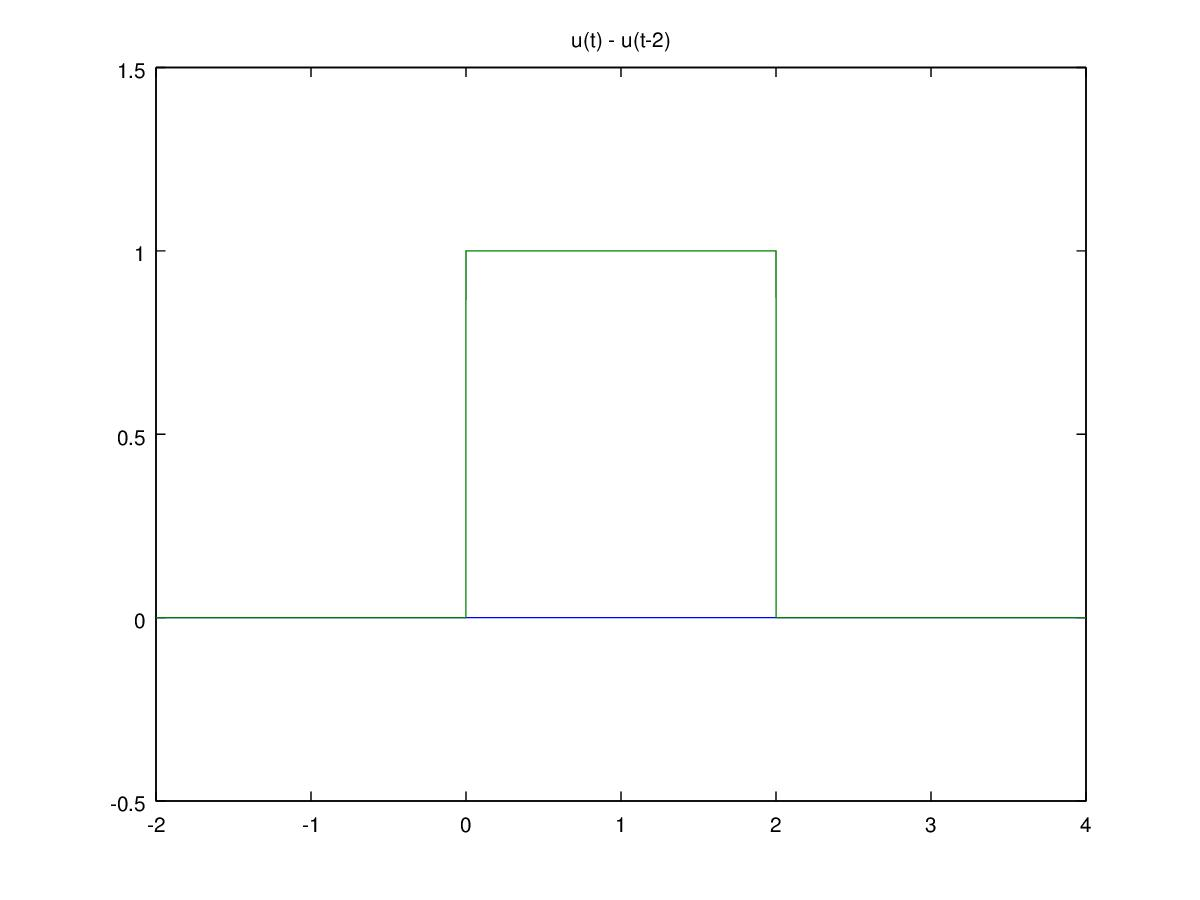
\includegraphics[height=3in]{./graphics/compesccont.eps}
	\caption{Composici\'{o}n de dos escalones para formar una se\~{n}al
		tipo pulso (tiempo continuo)}
	\label{compescconteps.1}
\end{figure}

\begin{figure}
	\centering
	
\includegraphics[height=3in]{./graphics/compcontuno.eps}
	\caption{Composici\'{o}n de se\~{n}ales (tiempo continuo)}
	\label{compcontunoeps}
\end{figure}

\begin{figure}
	\centering
	
\includegraphics[height=3in]{./graphics/compescdisc.eps}
	\caption{Composici\'{o}n de dos escalones para formar un par de
		impulsos (tiempo discreto)}
	\label{compescdisceps}
\end{figure}

\begin{figure}
	\centering
	
\includegraphics[height=3in]{./graphics/compcontdos.eps}
	\caption{Composici\'{o}n de se\~{n}ales (tiempo discreto)}
	\label{compcontdoseps}
\end{figure}

\begin{figure}
	\centering
	
\includegraphics[height=3in]{./graphics/comppreguno.eps}
	\caption{Pregunta sobre composici\'{o}n de se\~{n}ales (tiempo
		continuo)}
	\label{comppregunoeps}
\end{figure}

\begin{figure}
	\centering
	
\includegraphics[height=3in]{./graphics/comppregdos.eps}
	\caption{Pregunta sobre composici\'{o}n de se\~{n}ales (tiempo
		discreto)}
	\label{comppregdoseps}
\end{figure}

\section{Se\~{n}ales de tiempo discreto}

\subsection{El impulso unitario}

Hemos visto que el impulso unitario de tiempo discreto se define como 
\begin{equation}
        \delta \left[ n\right] =\left\{ 
\begin{array}{ll}
0, & n\neq 0, \\ 
1, & n=0.
\end{array}
\right.
\end{equation}

Vea la Fig. (\ref{epsimpunidisc}).

\begin{figure}
        \centering
        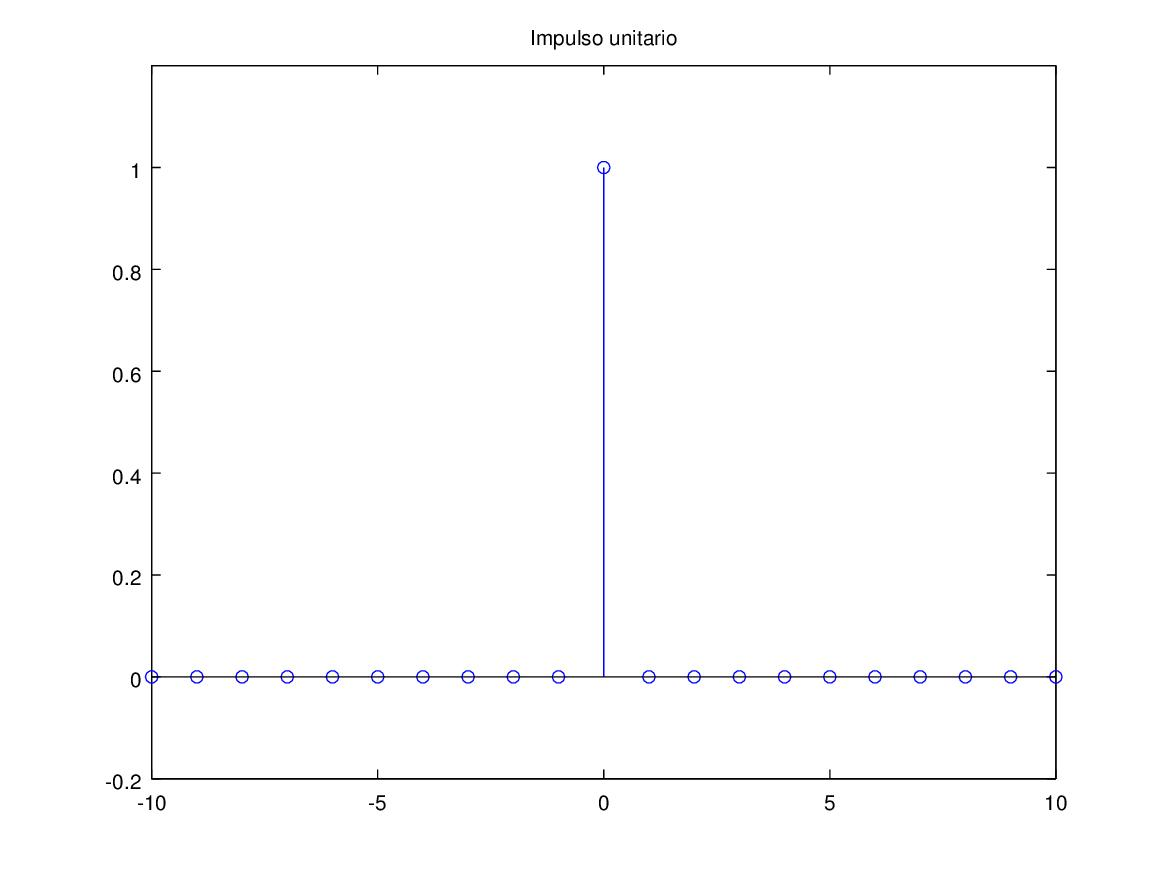
\includegraphics[height=2in]{./graphics/impunidisc.eps}
        \caption{Impulso unitario de tiempo discreto.}
        \label{epsimpunidisc}
\end{figure}

\subsection{El impulso unitario desplazado}

Desplazar un impulso unitario en el tiempo es sencillo. Veamos la
definci\'{o}n de $\delta[n-m]$ (La diferencia con la definici\'{o}n de
$\delta[n]$ aparece resaltada)
\begin{equation}
\delta[n\mathbf{-m}] = \left\{ \begin{array}{cc}
      1 & n  \mathbf{-m} = 0\\
      0 & n  \mathbf{-m} \neq 0 \end{array} 
  \right. \rightarrow
\delta[n\mathbf{-m}] = \left\{ \begin{array}{cc}
      1 & n  = \mathbf{m}\\
      0 & n  \neq \mathbf{m} \end{array} 
  \right.
\end{equation}

\subsection{El impulso multiplicado por un coeficiente}

La multiplicaci\'{o}n de un impulso unitario $\delta[n]$ por un
coeficiente $a$ se define como
\begin{equation}
a \, \delta[n] = \left\{ \begin{array}{cc}
      a & n = 0\\
      0 & n \neq 0 \end{array} 
  \right.
\end{equation}

\subsection{La suma de dos impulsos desplazados en el tiempo y
  multiplicados por coeficientes}

La suma de dos impulsos desplazados en el tiempo y multiplicados por
coeficientes es una combinaci\'{o}n lineal de impulsos. La podemos
definir de la siguiente forma
\begin{equation}
a_{1} \, \delta[n - m_{1}] + 
a_{2} \, \delta[n - m_{2}] = \left\{ \begin{array}{cc}
      a_{1} & n = m_{1}\\
      a_{2} & n = m_{2}\\
      0 & (n \neq m_{1}) \wedge (n \neq m_{2})  \end{array} 
  \right.
\end{equation}


\subsection{La suma de $N$ impulsos desplazados en el tiempos y
  multiplicados por coeficientes}

Podemos definir la suma de $N$ impulsos desplazados en el tiempo y multiplicados por
coeficientes $a_{k}$
\begin{equation}
x[n] = \sum_{k = 1}^{N} a_{k} \, \delta[n - k],
\end{equation}
donde para $m \in N$
\begin{equation}
x[m] = \sum_{k = 1}^{N} a_{k} \, \delta[m - k] = a_{m},
\end{equation}
porque solo donde $m = k$ se cumple $\delta[m - k] = \delta[0] = 1$ y por lo tanto hay un solo impulso igual a $1$ que multiplica al coeficiente $a_{m}$. Todos los otros coeficientes están multiplicados por $0$.

\subsection{La se\~ {n}al como combinaci\'{o}n lineal de impulsos}

\begin{enumerate}

\item Consideremos una sucesi\'{o}n de impulsos 
 $\delta\left[n - n_{0}\right]$, 
(ver Fig.(\ref{convoneeps}) y la Ec. (\ref{claveuno})), multiplicados por los
  respectivos coeficientes  $x\left[n_{0}\right]$, 
  \begin{eqnarray}
    x[-2]\delta \left[ n+2\right]   &=&     \left\{ \begin{array}{ll}
        x[-2],  & n=-2,                 \\ 
        0,      & n\neq -2,
      \end{array}
    \right.                                         \\
    x[-1]\delta \left[ n+1\right]   &=&     \left\{ \begin{array}{ll}
        x[-1],  & n=-1,                 \\ 
        0,      & n\neq -1,
      \end{array}
    \right.                                                 \\
    x[0]\delta \left[ n\right]      &=&     \left\{ \begin{array}{ll}
        x[0],   & n=0,                  \\ 
        0,      & n\neq 0,
      \end{array}
    \right.                                                 \\
    x[1]\delta \left[ n-1\right]    &=&     \left\{ \begin{array}{ll}
        x[1],   & n=1,                  \\ 
        0,      & n\neq 1,
      \end{array}
    \right.                                                 \\
    x[2]\delta \left[ n-2\right]   &=&     \left\{ \begin{array}{ll}
        x[2],   & n=2,                  \\ 
        0,      & n\neq 2,
      \end{array}
    \right.
  \end{eqnarray}
  y en general,
  \begin{equation}
    x[k]\delta \left[ n-k\right] =  \left\{ \begin{array}{ll}
        x[k],   & n=k,          \\ 
        0,      & n\neq k.
      \end{array}
    \right.
  \end{equation}

\item Como podemos ver en la Fig.(\ref{convoneeps}), la suma de
  impulsos desplazados en el tiempo multiplicados por coeficientes
  adecuados equivalen a cualquier se\~{n}al arbitraria $x[n]$.
  \begin{figure}
    \centering
    \includegraphics[width=3in]{./graphics/convone.eps}
    \caption{Una se\~{n}al como suma de impulsos desplazados en el
      tiempo multiplicados por coeficientes adecuados. Los impulsos
      desplazados $\delta[n-k]$ se representan $d[n-k]$.  S\'{o}lo se
      muestran tres impulsos por razones de espacio.}
    \label{convoneeps}
  \end{figure}
        
\item En efecto, agregando m\'{a}s impulsos desplazados y
  multiplicados adecuadamente podemos obtener una expresi\'{o}n que se
  puede escribir en forma general
  \begin{equation}
    x\left[ n\right] =
    \sum_{k=-\infty }^{\infty }x\left[ k\right] \delta \left[n-k\right] .  \label{cduna}
  \end{equation}

\item La Ec. (\ref{cduna}) corresponde a la representaci\'{o}n de una
  secuencia arbitraria $x[n]$ como
  \begin{itemize}
  \item una combinaci\'{o}n lineal de impulsos desplazados $\delta
    \left[ n-k\right]$,
                        
  \item donde los coeficientes de la combinaci\'{o}n lineal son los
    valores $x[k]$.
  \end{itemize}
                
\item Cada impulso desplazado $\delta \left[ n-k\right] $ act\'{u}a
  como selector: suponga que elegimos un valor $n=n_{0}$ y entonces
  tenemos que
  \begin{equation}
    x\left[ n_{0}\right] =
    \sum_{k=-\infty }^{\infty }x\left[ k\right] \delta \left[ n_{0}-k\right] .  
    \label{cddos}
  \end{equation}
                
\item Recordemos la definici\'{o}n de impulso
  \begin{equation}
    \delta \left[ n\right] =\left\{ 
      \begin{array}{cc}
        1, & n=0, \\ 
        0, & n\neq 0.
      \end{array}
    \right.
  \end{equation}
  El impulso ``vale'' $1$ cuando el \'{\i}ndice $n$ (lo que aparece
  entre corchetes) vale $0$. Note que en la ec. (\ref{cddos}) s\'{o}lo
  uno de los infinitos impulsos tiene un \'{\i}ndice nulo,
  espec\'{\i}ficamente
  \begin{equation}
    n_{0}-k=0.
  \end{equation}
  Entonces, de todos los infinitos t\'{e}rminos s\'{o}lo uno es no
  nulo ($k=n_{0})$.  As\'{\i} obtenemos la igualdad
  \begin{equation}
    x\left[ n_{0}\right] =x\left[ n_{0}\right] .
  \end{equation}

\item La utilidad de la ecuaci\'{o}n (\ref{cduna}) es que expresa una
  secuencia
  \begin{equation}
    ...x[-3],x[-2],x[-1],x[0],x[1],x[2],x[3]...
  \end{equation}
  como una sumatoria.

\end{enumerate}

\subsection{La se\~{n}al multiplicada con un impulso}

\begin{enumerate}
\item Consideremos una se\~{n}al $x\left[ n\right]$ a la que
  multiplicamos por un impulso $\delta\left[ n - n_{0}\right]$. 
Hemos probado que
\begin{equation}
x\left[ n\right] \, \delta\left[ n - n_{0}\right] = 
x\left[ n_{0}\right] \, \delta\left[ n - n_{0}\right].
\end{equation}

\item Recordemos que el impulso desplazado $\delta\left[ n - n_{0}\right]$
  act\'{u}a como ``selector'' al multiplicar a una se\~{n}al $x[n]$:
  la \'{u}nica muestra de $x[n]$ multiplicada por $1$ es $x[n_{0}]$,
  todas las dem\'{a}s se multiplican por $0$.

\end{enumerate}

\subsection{Escalado temporal}

\begin{enumerate}
\item Supongamos que tenemos una se\~{n}al $x[n]$ y la usamos para
generar otra se\~{n}al 
\begin{equation}
y[n] = x[3 \, n]. \label{escaladotemporaluno}
\end{equation}
\textquestiondown Qu\'{e} significa la
  Ec. (\ref{escaladotemporaluno})?
Analizemos la siguiente tabla, 

\begin{tabular}{ccc}
$n$ & $x[n]$ & $y[n] = x[3 \, n]$? \\
0   &  $x[0]$ & $x[0]$ \\
& & \\
1   &  $x[1]$ & $x[3]$ \\
& & \\
2   &  $x[2]$ & $x[6]$ \\
& & \\
3   &  $x[3]$ & $x[9]$ \\
& & \\
4   &  $x[4]$ & $x[12]$ \\
& & \\
5   &  $x[5]$ & $x[15]$ \\
& & \\
6   &  $x[6]$ & $x[18]$ \\
... &  ... & ...
\end{tabular}

\item Supongamos que tenemos una se\~{n}al $x[n]$ y la usamos para
generar otra se\~{n}al 
\begin{equation}
y[n] = x[\frac{1}{3} \, n]. \label{escaladotemporaldos}
\end{equation}
\textquestiondown Qu\'{e} significa la Ec. (\ref{escaladotemporaldos})?
Analizemos la siguiente tabla

\begin{tabular}{ccc}
$n$ & $x[n]$  & $x[\frac{n}{3}]$ \\
& & \\
0   &  $x[0]$ & $x[\frac{0}{3}]$ \\
& & \\
1   &  $x[1]$ & $x[\frac{1}{3}]$ ?\\
& & \\
2   &  $x[2]$ & $x[\frac{2}{3}]$ ?\\
& & \\
3   &  $x[3]$ & $x[\frac{3}{3}]$ \\
& & \\
4   &  $x[4]$ & $x[\frac{4}{3}]$ ?\\
& & \\
5   &  $x[5]$ & $x[\frac{5}{3}]$ ?\\
& & \\
6   &  $x[6]$ & $x[\frac{6}{3}]$ \\
& & \\
7   &  $x[7]$ & $x[\frac{7}{3}]$ ?\\
... &  ... & ...
\end{tabular}

Como podemos ver, el problema es que el \'{\i}ndice de una se\~{n}al
de tiempo discreto debe ser un n\'{u}mero entero. Por lo tanto,
deber\'{\i}amos emplear la siguiente definici\'{o}n
\begin{equation}
y[n] = \left\{ \begin{array}{cc}
    x[\frac{n}{3}],      & n = 3 \, m \\
    0,         & n = 3 \, m + 1\\
    0,         & n = 3 \, m + 2
\end{array} \right.
\end{equation}
$\forall m \in N$.

\end{enumerate}

\subsection{Tiempo inverso}

El caso de escalado temporal m\'{a}s sencillo es el del ``viaje al
pasado''. En este caso $y[n] = x[-n]$. Es algo como reproducir un audio "al revés".

Esta es una operación usada en dos casos. Existe un dispositivo denominado scrambler que se puede aplicar a un teléfono: divide el audio en segmentos y después los invierte en tiempo, segmento por segmento, antes de enviarlos por el canal de comunicación. En el otro lado del canal, un dispositivo similar recupera la señal original con el mismo proceso. La idea es que "nadie" pueda espiar la conversación, o mejor dicho que nadie la espíe fácilmente.
También hubo rumores que si se reproducen en tiempo inverso las canciones de rock se pueden oir mensajes ocultos.

Un ejemplo con matlab
\begin{verbatim}
	n = 1:5;
	x = randn(1, 5);
	subplot(2,1,1); stem(n, x); 
	subplot(2,1,2); stem(-n, x);
\end{verbatim}

\subsection{Desplazamiento en el tiempo}

\begin{enumerate}
\item Supongamos una se\~{n}al $x[n]$. Podemos desplazarla en el tiempo
haciendo $y[n] = x[n - n_{0}]$.

\item Por ejemplo, si $x_{1}[n] = cos(2 \, \pi \, \frac{2}{5} \, n)$,
  podemos obtener su versi\'{o}n desplazada cuatro muestras como
  $y_{1} = x_{1}[n - 4] =  cos(2 \, \pi \, \frac{2}{5} \, (n - 4))$.
\end{enumerate}

\subsection{Tren de impulsos}

\begin{enumerate}
\item El impulso unitario est\'{a} definido como
\begin{equation}
\delta[n] = \left\{ \begin{array}{cc}
1 & n = 0, \\
0 & n \neq 0.
\end{array}
\right.
\end{equation}

\item Podemos desplazar el impulso unitario definiendo
\begin{equation}
\delta[n - n_{0}] = \left\{ \begin{array}{cc}
1 & n = n_{0},  \\
0 & n \neq n_{0}.
\end{array}
\right.
\end{equation}

\item Por lo tanto, la siguiente definici\'{o}n 
\begin{equation}
\delta[n - k \, n_{0}] = \left\{ \begin{array}{cc}
1 & n = k \, n_{0},  \\
0 & n \neq k \, n_{0}.
\end{array}
\right.
\end{equation}
donde $k$ es un n\'{u}mero entero, 
nos da impulsos ubicados en m\'{u}ltiplos enteros de $n_{0}$.

\item Si sumamos todos los impulsos obtenidos en el punto anterior,
  obtenemos el tren de impulsos
\begin{equation}
x[n] = \sum_{k=-\infty}^{\infty} \delta[n - k \, n_{0}].
\end{equation}

\end{enumerate}


\section{Se\~{n}ales de tiempo continuo}

\subsection{El pulso}

Un pulso unitario de tiempo continuo $p(t)$ de duraci\'{o}n $\tau$ se define
como una diferencia de escalones unitarios con un factor $\frac{1}{\tau}$
\begin{equation}
  p(t) = \frac{1}{\tau} \left(u(t) - u(t - \tau) \right),
\end{equation}
donde $\tau > 0$.

  \begin{figure}
    \centering
    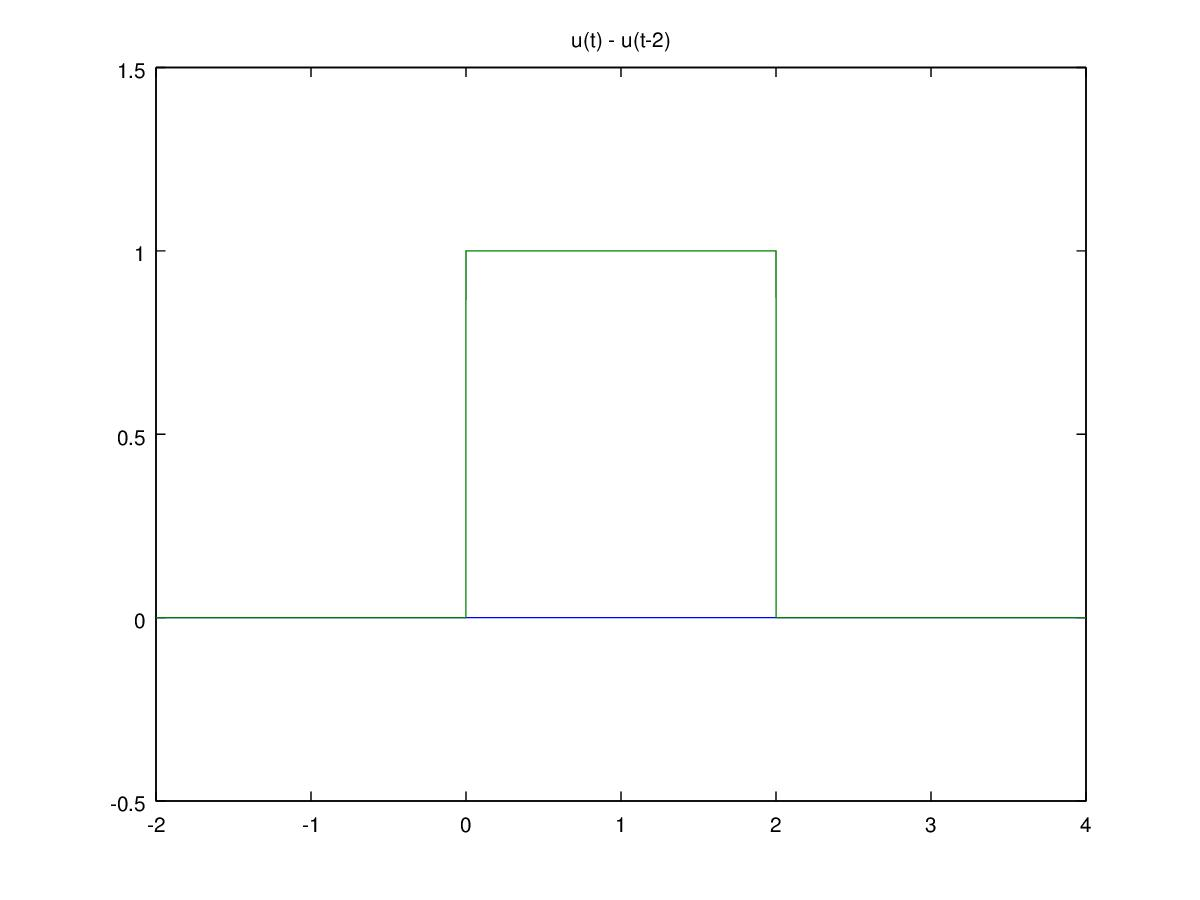
\includegraphics[width=3in]{./graphics/compesccont.eps}
    \caption{Pulso de tiempo continuo con $\tau = 2$}
    \label{compescconteps.3}
  \end{figure}

\subsection{El pulso desplazado}

Un pulso unitario de tiempo continuo $p(t)$ de duraci\'{o}n $\tau$
desplazado en el tiempo $t_{0}$ se define como una diferencia de escalones
unitarios desplazados en el tiempo $t_{0}$
\begin{equation}
  p(t-t_{0}) = \frac{1}{\tau} \, \left(u(t-t_{0}) - u(t - t_{0} -
    \tau) \right).
\end{equation}

\subsection{El impulso como l\'{\i}mite del pulso}

Cuando $\tau$ tiende a $0$, el ancho del impulso tiende a $0$, su
altura tiende a $\infty$, y su \'{a}rea se mantiene igual a $1$.

  \begin{figure}
    \centering
    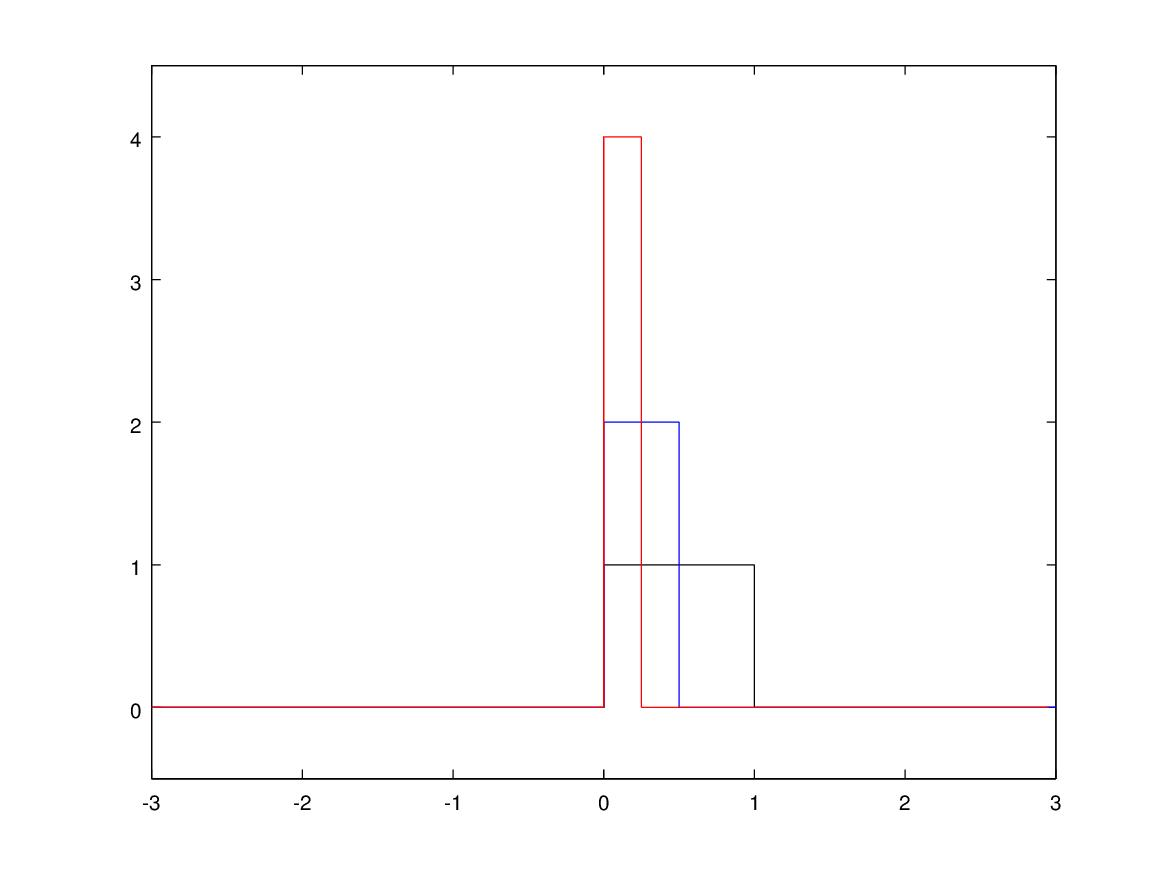
\includegraphics[width=3in]{./graphics/sucimpcont.eps}
    \caption{Impulso como l\'{\i}mite de una sucesi\'{o}n de impulsos}
    \label{sucimpconteps.3}
  \end{figure}

  \begin{figure}
    \centering
    \includegraphics[width=3in]{./graphics/lecture02_tex_gr7.eps}
    \caption{Otra funci\'{o}n de \'{a}rea unitaria (y van dos)}
    \label{lecture02texgr7eps.3}
  \end{figure}

  \begin{figure}
    \centering
    \includegraphics[width=3in]{./graphics/lecture02_tex_gr8.eps}
    \caption{Otra funci\'{o}n de \'{a}rea unitaria (y van tres)}
    \label{lecture02texgr8eps.3}
  \end{figure}

\subsection{La se\~{n}al aproximada por una combinaci\'{o}n lineal de pulsos}

  \begin{figure}
    \centering
    \includegraphics[width=3in]{./graphics/contconv222.eps}
    \caption{Se\~{n}al aproximada por combinaci\'{o}n lineal de pulsos}
    \label{contconv222eps}
  \end{figure}

La se\~{n}al $x(t)$ puede aproximarse como una combinaci\'{o}n lineal
de pulsos desplazados en el tiempo como puede verse en la figura
(\ref{contconv222eps}), o anal\'{\i}ticamente con mediante los
siguientes pasos:
\begin{enumerate}
\item Desplaze los pulsos en el tiempo
\begin{equation}
        \begin{array}{c}
                ...                                             \\ 
                \delta _{\Delta }\left( t+\Delta \right) =
                        \left\{ \begin{array}{l}
                                        \frac{1}{\Delta },      \\ 
                                        0,
                                \end{array}
                                \begin{array}{l}
                                        -\Delta \leq t<0,       \\ 
                                        \left( t<-\Delta \right) \vee \left( 0\leq t\right) ,
                                \end{array}
                        \right.                                 \\ 
                \delta _{\Delta }\left( t\right) =
                        \left\{ \begin{array}{l}
                                        \frac{1}{\Delta },      \\ 
                                        0,
                                \end{array}
                                \begin{array}{l}
                                        0\leq t<\Delta ,        \\ 
                                        \left( t<0\right) \vee \left( \Delta \leq t\right) ,
                                \end{array}
                        \right.                                 \\ 
                \delta _{\Delta }\left( t-\Delta \right) =
                        \left\{ \begin{array}{l}
                                        \frac{1}{\Delta },      \\ 
                                        0,
                                \end{array}
                                \begin{array}{l}
                                        \Delta \leq t<2\Delta , \\ 
                                        \left( t<\Delta \right) \vee \left( 2\Delta \leq t\right) ,
                                \end{array}
                        \right.                                 \\ 
                ...                                             \\ 
                \delta _{\Delta }\left( t-k\Delta \right) =
                        \left\{ \begin{array}{l}
                                        \frac{1}{\Delta },      \\ 
                                        0,
                                \end{array}
                         \begin{array}{l}
                            k\Delta \leq t<\left( k+1\right) \Delta , \\ 
                              \left( t<k\Delta \right) \vee \left( \left( k+1\right) \Delta \leq t\right) .
                         \end{array}
               \right.
        \end{array}
\end{equation}

\item Multiplicando por $x\left( k\Delta \right) \Delta $ al $k-\acute{e}simo$ pulso se obtiene 
\begin{equation}
        \begin{array}{c}
                        ...                                                                    \\ 
                        x\left( -\Delta \right) \delta _{\Delta }\left( t+\Delta \right) \Delta =
                                \left\{ \begin{array}{l}
                                                \frac{x\left( -\Delta \right) }{\Delta }\Delta ,        \\ 
                                                0,
                                        \end{array}
                                        \begin{array}{l}
                                           -\Delta \leq t<0,                                       \\ 
                                          \left( t<-\Delta \right) \vee \left( 0\leq t\right) ,
                                        \end{array}
                                \right.                                                                 \\ 
                        x\left( 0\right) \delta _{\Delta }\left( t\right) \Delta =
                                \left\{ \begin{array}{l}
                                                \frac{x\left( 0\right) }{\Delta }\Delta ,               \\ 
                                                0,
                                        \end{array}
                                        \begin{array}{l}
                                                0\leq t<\Delta ,                                        \\ 
                                                \left( t<0\right) \vee \left( \Delta \leq t\right) ,
                                        \end{array}
                                \right.                                                                 \\ 
                        x\left( \Delta \right) \delta _{\Delta }\left( t-\Delta \right) \Delta =
                                \left\{ \begin{array}{l}
                                                \frac{x\left( \Delta \right) }{\Delta }\Delta ,         \\ 
                                                0,
                                        \end{array}
                                        \begin{array}{l}
                                                \Delta \leq t<2\Delta ,                                 \\ 
                                                \left( t<\Delta \right) \vee \left( 2\Delta \leq t\right) ,
                                        \end{array}
                                \right.                                                                 \\ 
                        ... \\ 
                        x\left( k\Delta \right) \delta _{\Delta }\left( t-k\Delta \right) \Delta =
                                \left\{ \begin{array}{l}
                                                \frac{x\left( k\Delta \right) }{\Delta }\Delta ,        \\ 
                                                0,
                                        \end{array}
                       \begin{array}{l}
                             k\Delta \leq t<\left( k+1\right) \Delta ,               \\ 
                             \left( t<k\Delta \right) \vee \left( \left( k+1\right) \Delta \leq t\right) .
                       \end{array}
                       \right.
        \end{array}
\end{equation}
\item Observe que un valor dado de $t$ (por ejemplo $t_{0})$ s\'{o}lo puede pertenecer a \textbf{un} intervalo 
$k\Delta \leq t<\left( k+1\right) \Delta,$ por lo tanto para $t_{0}$ solo uno de los productos puede ser 
distinto de $0$. Sumando los infinitos productos obtenemos 
\begin{equation}
   x_{\Delta }\left( t\right) =
     \sum_{k=-\infty }^{\infty }x\left( k\Delta \right) \delta
     _{\Delta }\left( t-k\Delta \right) \Delta . \label{funcaspulsessum}
\end{equation}
\end{enumerate}

\subsection{La se\~{n}al como combinaci\'{o}n lineal de impulsos}

Observe que en la ecuaci\'{o}n (\ref{funcaspulsessum}) cuando 
$\Delta$ tiende a cero $x_{\Delta }\left(t\right)$ tiende a 
$x\left(t\right) .$

\begin{equation}
        x\left( t\right) =      
\begin{array}{l}
    Lim \\ 
    \Delta \rightarrow 0
\end{array}
x_{\Delta }\left( t\right) = 
\begin{array}{l}
    Lim \\ 
    \Delta \rightarrow 0
\end{array}
   \sum_{k=-\infty }^{\infty }x\left( k\Delta \right) \delta _{\Delta }\left(t-k\Delta \right) \Delta .
\end{equation}
Adem\'{a}s, cuando $\Delta $ tiende a cero, la sumatoria se convierte en una integral 
\begin{equation}
        x\left( t\right) =\int_{-\infty }^{\infty }x\left( \tau \right) \delta\left( t-\tau \right) d\tau .
\end{equation}
Notemos que por la propiedad del muestreo, debe cumplirse 
\begin{equation}
   x\left( \tau \right) \delta \left( t-\tau \right) = 
     x\left( t\right) \delta \left( t-\tau \right) ,
\end{equation}
y en ese caso 
\begin{equation}
 x\left( t\right) = 
  x\left( t\right) \left( \int_{-\infty }^{\infty }\delta \left( t-\tau \right) d\tau \right),
\end{equation}
con lo que hemos probado que una funci\'{o}n $x(t)$ puede escribirse
como una combinaci\'{o}n lineal de impulsos.

%\subsection{La se\~{n}al multiplicada con un impulso}
%
%Para evaluar la multiplicaci\'{o}n de una se\~{n}al $x(t)$ y un impulso $\delta_{t - t_{0}}$
%consideremos la ecuaci\'{o}n (\ref{funcaspulsessum}). 
%
%\begin{enumerate}
%\item Podemos escribir
%\begin{equation}
%   x_{\Delta }\left( t\right) \, \delta_{\Delta }\left( t-k_{0} \, \Delta \right) = 
%     \left( \sum_{k=-\infty }^{\infty }x\left( k \, \Delta \right) 
%\delta_{\Delta }\left( t-k \, \Delta \right) \Delta \right) \,
%\delta_{\Delta }\left( t-k_{0} \, \Delta \right).
%\end{equation}
%
%\item Esta \'{u}ltima ecuaci\'{o}n es equivalente a 
%\begin{equation}
%   x_{\Delta }\left( t\right) \, \delta_{\Delta }\left( t-k_{0} \, \Delta \right) = 
%   x\left( k_{0} \, \Delta \right) \, 
%  \delta_{\Delta }\left( t-k_{0} \, \Delta \right) \,    
%  \delta_{\Delta }\left( t-k_{0} \, \Delta \right),
%\end{equation}
%pues el pulso en $k_{0} \, \Delta$, al multiplicar a otros pulsos 
%$k \neq k_{0}$, los anula. 
%
%\item Multiplicando ambos lados de la ecuaci\'{o}n por $\Delta$ tenemos
%\begin{equation}
%   x_{\Delta }\left( t\right) \, \delta_{\Delta }\left( t-k_{0} \,
%     \Delta \right) \, \Delta = 
%   x\left( k_{0} \, \Delta \right) \delta_{\Delta }\left( t-k_{0} \,
%     \Delta \right) \, \Delta \, \delta_{\Delta }\left( t-k_{0} \,
%     \Delta \right) \, \Delta,
%\end{equation}
%
%\item Finalmente, tomado el l\'{\i}mite de $\Delta$ tendiendo a $0$ obtenemos
%\begin{equation}
%  \begin{array}{c}
%     Lim \\
%     \Delta \rightarrow 0,
%  \end{array}
%   x_{\Delta }\left( t\right) \, \delta_{\Delta }\left( t-k_{0} \,
%     \Delta \right) \, \Delta = x(t) \, \delta(t - t_{0}),
%\end{equation}
%y
%\begin{equation}
%  \begin{array}{c}
%     Lim \\
%     \Delta \rightarrow 0,
%  \end{array}
%   x\left( k_{0} \, \Delta \right) \delta_{\Delta }\left( t-k_{0} \,
%     \Delta \right) \, \Delta \, \delta_{\Delta }\left( t-k_{0} \,
%     \Delta \right) \, \Delta = x(t_{0}) \, \delta(t - t_{0}).
%\end{equation}
%
%\end{enumerate}
%
%Por lo tanto, $x(t) \, \delta(t - t_{0}) = x(t_{0}) \, \delta(t - t_{0})$.



\subsection{Desplazamiento en el tiempo}

\begin{enumerate}
\item Supongamos una se\~{n}al $x(t)$. Podemos desplazarla en el tiempo
haciendo $y(t) = x(t - t_{0})$.

\item Por ejemplo, si $x_{1}(t) = cos(2 \, \pi \, \frac{2}{10} \, t)$,
  podemos obtener su versi\'{o}n desplazada cuatro unidades de tiempo como
  $y_{1}(t) = x_{1}(t - 4) =  cos(2 \, \pi \, \frac{2}{10} \, (t - 4))$.
\end{enumerate}


\subsection{Escalado temporal}

\begin{enumerate}
\item El escalado temporal es reemplazar la variable independendiente $t$
por otra variable a la que llamaremos $v$. La relaci\'{o}n de estas
variables est\'{a} dada por una escala que simbolizaremos con la letra
$a$. Por ejemplo, $t = a \, v$.

\item Considermos la se\~{n}al $x(t) = sen(2 \, \pi \, t)$. Podemos
  realizar el escalado temporal $t = 2  \, v$, para obtener $y(v) =
  sen(4 \, \pi \, v)$.

\end{enumerate}

\subsection{Tiempo inverso}

Un caso especial de escalado temporal es cuando la escala es
negativa. Por ejemplo, con $t = - v$, obtenemos el denominado tiempo inverso.

\subsection{Tren de impulsos}

\begin{enumerate}
\item Supongamos una serie de impulsos desplazados en el tiempo $\delta(t)$,
$\delta(t - T)$, $\delta(t - 2 \, T)$, $\delta(t - 3 \, T)$ y en
general $\delta(t - k \, T)$, para $k$ entero. 

\item El par de impulsos sucesivos $\delta(t - k \, T)$ y $\delta(t -
  (k+1) \, T)$ esta separado por un intervalo de tiempo $T$.

\item El tren de impulsos es igual a a la sumatoria de todos los
  impulsos $\delta(t - k \, T)$, para $k$ entero
\begin{equation}
\Pi_{T}(t) = \sum_{k=-\infty}^{\infty} \delta(t - k \, T),
\end{equation}
donde los impulsos son no nulos en $t = k \, T$.
\end{enumerate}

\subsection{Muestreo}

El muestreo digital de una señal analógica (de tiempo continuo) nos permite obtener una señal de tiempo discreto.
Si cumplimos ciertas condiciones, que vamos a estudiar durante este curso, 
es posible realizar un proceso inverso que nos permite recuperar la señal de tiempo continuo original.

El muestreo ideal es una función que toma los valores de $x(t)$ en los instantes $t = k \, T$, y $0$ para todo $t \neq k \, T$, 
donde $T$ es el período de muestreo y $k$ es una variable entera. Matemáticamente, podemos representar la operación de muestreo como 
la multiplicación de una señal $x(t)$ con un tren de impulsos de período $T$
\begin{equation}
 y(t) = x(t) \times \Pi_{T}(t) = x(t) \times \left( 
 \sum_{k=-\infty}^{\infty} \delta(t - k \, T)
 \right).
\end{equation}
Entonces
\begin{equation}
	y(t) =  
	\left( 
	\sum_{k=-\infty}^{\infty} x(t) \times \delta(t - k \, T)
	\right) =
    \sum_{k=-\infty}^{\infty} x(k \, T) \times \delta(t - k \, T).
\end{equation}


\section{Operaciones útiles, para tiempo discreto}

% Lathi, página 287

\subsection{Decimación}

Supongamos una señal $x[n]$. La decimación de una señal $x[n]$ es la generación de una nueva señal $y[n]$ mediante la eliminación de ciertas muestras de $x[n]$. 
Para eso multiplicamos $x[n]$ por
\begin{equation}
	y[n] = x[n] \times \left( \sum_{k=-\infty}^{\infty} \delta[n - k \, N]\right),
\end{equation}
Si escribimos
\begin{equation}
	y[n] = \sum_{k=-\infty}^{\infty} x[n] \times \delta[n - k \, N] =
	\sum_{k=-\infty}^{\infty} x[k \, N] \times \delta[n - k \, N].
\end{equation}
es evidente que para $n = q \, N + r$, $q \in N$, $0 < r < N$ debe ser $y[n] = 0$, 

\subsection{Interpolación}

Supongamos una señal $x[n]$. La interpolación de una señal $x[n]$ es la generación de una nueva señal $y[n]$ mediante la introducción de nuevas muestras 
calculadas, por ejemplo, como promedios de dos muestras consecutivas de $x[n]$. Por ejemplo,
\begin{equation}
	y[0] = x[0],
\end{equation}
\begin{equation}
	y[1] = (x[0] + x[1]) / 2,
\end{equation}
\begin{equation}
	y[2] = x[1],
\end{equation}
\begin{equation}
	y[3] = (x[1] + x[2]) / 2,
\end{equation}
y así sucesivamente.

Esta no es la única forma de interpolar. Es sólo un ejemplo de un tema que vamos a ver con más detenimiento cuando veamos transformada de Fourier.

 % Composici\'{o}n de se\~{n}ales

\chapter{Sistemas (y se\~{n}ales)}

\section{Introducci\'{o}n}

\subsection{Definiciones}

\begin{enumerate}
\item Las se\~{n}ales son magnitudes naturales variables portadoras
  de informaci\'{o}n entre sistemas, representadas por funciones de
  variables independientes.

\item Los sistemas son conjuntos de partes que interact\'{u}an entre
  si, con un prop\'{o}sito com\'{u}n.

\item Los sistemas reciben se\~{n}ales de entrada para entregar
  se\~{n}ales de salida.

\item Sistema de tiempo continuo es aquel que recibe, procesa y
  entrega solamente se\~{n}ales de tiempo continuo.

\item Sistema de tiempo discreto es aquel que recibe, procesa y entrega
  solamente se\~{n}ales de tiempo discreto.

\item Sistema h\'{\i}brido es aquel que recibe, procesa y entrega se\~{n}ales
  de tiempo continuo y discreto.

\item Los sistemas pueden representarse mediante relaciones entre las
  se\~{n}ales de entrada y salida.

\item En el caso de sistemas de tiempo continuo, simbolizados
    \begin{equation}
      x(t) 
      \begin{array}{l}
        S               \\ 
        \rightarrow
      \end{array}
      y(t),
    \end{equation}
    podemos emplear los siguientes operadores matem\'{a}ticos para describirlos
    \begin{enumerate}
    \item Ecuaciones algebraicas
      \begin{equation}
        F(t, x(t), y(t)) = 0,
      \end{equation}
      donde $x(t)$ es la entrada e $y(t)$ es la salida del sistema. Por ejemplo,
      \begin{equation}
         y(t) - x(t) \, cos(2 \, t) = 0.
      \end{equation}
                                
    \item Ecuaciones diferenciales donde $x(t)$ es la entrada e $y(t)$ es la salida del sistema. Por ejemplo,
      \begin{equation}
        \frac{d y(t)}{dt} + 2 \, y(t) - x(t) = 0.
      \end{equation}
    \end{enumerate}
        
  \item En el caso de sistemas de tiempo discreto, simbolizados
    \begin{equation}
      x\left[ n\right] 
      \begin{array}{l}
        S               \\ 
        \rightarrow
      \end{array}
      y\left[ n\right] ,
    \end{equation}
    podemos emplear los siguientes operadores matem\'{a}ticos para describirlos
    \begin{enumerate}
    \item Ecuaciones algebraicas
      donde $x[n]$ es la entrada e $y[n]$ es la salida del sistema. Por ejemplo,
      \begin{equation}
         y[n] - x[n] \, 2^{-n} = 0.
      \end{equation}
                                
    \item Ecuaciones de diferencias finitas donde $x[n]$ es la entrada e $y[n]$ es la salida del sistema. Por ejemplo
      \begin{equation}
          y[n] - x[n] + x[n-1] - \frac{x[n-1]}{2} - y[n-1] - 2 \, y[n-2] + 4 \, y[n-3] = 0.
      \end{equation}
    \end{enumerate}

\item Las descripciones de sistemas, ya sean ecuaciones algebraicas,
  ecuaciones diferenciales, o de diferencias son modelos
  matem\'{a}ticos del sistema, y los podemos usar para an\'{a}lisis y
  dise\~{n}o.

\end{enumerate}

\subsection{Ejemplos}

\subsubsection{Divisor resistivo de tensi\'{o}n}
Supongamos que tenemos un divisor resistivo de tensi\'{o}n donde la
relaci\'{o}n entre la tensi\'{o}n de entrada $v_{e} \left( t \right)$
y salida $v_{s} \left( t \right)$ es la ecuaci\'{o}n
\begin{equation}
  V_{s}\left( t \right) = \frac{R_{2}}{R_{1} + R_{2}} \, V_{e}\left( t \right).      \label{divires}
\end{equation}
Esta es una ecuaci\'{o}n algebraica de tiempo continuo.  Ver Figura
(\ref{circuitoeps})

\subsubsection{Circuito RC Serie}
Supongamos que tenemos un circuito RC serie descripto por la
ecuaci\'{o}n diferencial
\begin{equation}
  \frac{dv_{c}\left( t\right) }{dt}+\frac{1}{R \, C} \, v_{c}\left( t\right) =
  \frac{1}{R \, C} \, v_{s}\left( t\right) . \label{rcserie}
\end{equation}
donde
\begin{enumerate}
\item $v_{c}(t)$ tensi\'{o}n en el capacitor,
\item $v_{s}\left( t\right) $ tensi\'{o}n en la fuente,
\item $R$ valor de la resistencia,
\item $C$ valor del capacitor.
\end{enumerate}
Ver Figura (\ref{circuitoeps}).

\subsubsection{Un negocio}
Supongamos que el due\~{n}o de un negocio repone todos los d\'{\i}as
la mercader\'{\i}a.  La ecuaci\'{o}n que describe la relaci\'{o}n
entre la cantidad de mercader\'{\i}a que entra en el dep\'{o}sito y el
dinero necesario para comprarla es
\begin{equation}
  t[n] = p \, (m - x[n]).
\end{equation}
donde
\begin{enumerate}
\item $x[n]$ es la cantidad de mercader\'{\i}a en el dep\'{o}sito,
\item $m$ la cantidad m\'{a}xima de mercader\'{\i}a que puede tener
  guardada,
\item $p$ el precio unitario,
\item $t[n]$ el pago por la compra del d\'{\i}a $n$.
\end{enumerate}
Esta es una ecuaci\'{o}n algebraica de tiempo discreto.

\subsubsection{Cuenta bancaria}
Supongamos que tenemos una cuenta bancaria en la que obtenemos cierto
inter\'{e}s mensual por mantener cierto dep\'{o}sito de dinero.  La
ecuaci\'{o}n de diferencias que nos dice cuanto dinero tendremos el
pr\'{o}ximo mes es
\begin{equation}
  y\left[n+1\right] = (1+c/100) \, y[n]+x[n],
\end{equation}
donde
\begin{enumerate}
\item $y[n+1]$ dinero en la cuenta el pr\'{o}ximo mes,
\item $y[n]$ dinero en la cuenta este mes,
\item $x[n]$ dinero depositado o extra\'{\i}do este mes,
\item $c$ inter\'{e}s.
\end{enumerate}
Esta es una ecuaci\'{o}n de diferencias y por lo tanto, de tiempo
discreto.

\subsubsection{C\'{a}lculo de ra\'{\i}ces de polin\'{o}mios}
Supongamos que tenemos que calcular \textbf{una} ra\'{\i}z del
polin\'{o}mio
\begin{equation}
  Q(x) = 0.
\end{equation}
Para obtener \textbf{una} soluci\'{o}n podemos escribir la ecuaci\'{o}n de
diferencias
\begin{equation}
  x_{k+1} = x_{k} - \left(\frac{Q(x)}{\frac{d Q(x)}{dx}}\right)_{x=x_{k}}.
\end{equation}
Si damos a $x_{0}$ un valor suficientemente cercano a \textbf{la}
ra\'{\i}z buscada del polin\'{o}mio $Q(x)$, obtendremos una secuencia
que converge r\'{a}pidamente. Por ejemplo, si consideramos el polinomio
\begin{equation}
Q(x) = x^{2} - 2 = 0, 
\end{equation}
calcularemos la raíz cuadrada de $2$. Por lo tanto, iteremos la ecuaci\'{o}n de diferencias
\begin{equation}
  x_{k+1} = \frac{2 + x^{2}_{k}}{2 x_{k}}, \qquad x_{0}   = 2,
\end{equation}
para obtener los primeros cinco valores de la secuencia
\begin{equation}
  \begin{array}{llllll}
    2 & 1.5 & 1.41667 & 1.41422 & 1.41421 & ...
  \end{array}
\end{equation}
que como vemos se acerca r\'{a}pidamente al resultado correcto.

\section{Modelos}

Necesitamos describir los sistemas con los que trabajamos para poder
analizarlos, verificar sus propiedades, o para dise\~{n}ar nuevos
sistemas. Como ya vimos, podemos usar ecuaciones diferenciales y
ecuaciones de diferencias.

\subsection{Ecuaciones diferenciales}

Consideremos una ecuaci\'{o}n diferencial
\begin{equation}
  \frac{d^{N} y(t)}{dt^{N}} + 
  \sum_{i=0}^{N-1} a_{i} \, \frac{d^{i} y(t)}{dt^{i}} = 
  \sum_{j=0}^{M} b_{i} \, \frac{d^{j} x(t)}{dt^{j}},
\end{equation}
donde $x(t)$ es la entrada, $y(t)$ es la salida, y los coeficientes
$a_{i}$ y $b_{j}$ son constantes reales, $N \geq 1$, $M \geq
0$, $N > M$. Por ejemplo,
\begin{equation}
\frac{dy^{3}(t)}{dt} + 3 \, \frac{dy^{2}(t)}{dt^{2}} 
+ 2 \, \frac{dy(t)}{dt}
+ y(t) 
= x(t).
\end{equation}
Las ecuaciones diferenciales pueden escribirse como un sistema de ecuaciones
diferenciales de primer orden denominadas ecuaciones de estado empleando 
variables de estado. 
Una posible definici\'{o}n de las variables de estado es la siguiente
\begin{eqnarray}
  v_{1}   &=& y(t),                                               \\
  v_{k+1} &=& \frac{dv_{k}}{dt} = \frac{d^{k}y}{dt^{k}},  \, 0 < k < N .
\end{eqnarray}
Con esta definici\'{o}n podemos escribir las ecuaciones de estado
\begin{eqnarray}
  \frac{dv_{k}}{dt} &=& v_{k+1},  \, 1 \leq k < N,  \\
  \frac{dv_{N}}{dt} &=& G(t, x(t), v_{1}, v_{2},...,v_{N}).
\end{eqnarray}
Por ejemplo, para
\begin{equation}
\frac{dy^{3}(t)}{dt} + 3 \, \frac{dy^{2}(t)}{dt^{2}} 
+ 2 \, \frac{dy(t)}{dt}
+ y(t) 
= x(t),
\end{equation}
definimos
\begin{equation}
v_{1} = y(t),
\end{equation}
\begin{equation}
\frac{dv_{1}}{dt} = v_{2} = \frac{dy(t)}{dt},
\end{equation}
\begin{equation}
\frac{dv_{2}}{dt} = v_{3} = \frac{dy^{2}(t)}{dt^{2}},
\end{equation}
\begin{equation}
\frac{dv_{3}}{dt} = \frac{dy^{3}(t)}{dt^{3}} = -v_{1} - 2 \, v_{2} - 3 \, v_{3} + x(t).
\end{equation}
En forma matricial
\begin{equation}
\left[ \begin{array}{c}
\frac{dv_{1}}{dt} \\
\frac{dv_{2}}{dt} \\
\frac{dv_{3}}{dt}
\end{array} \right] 
= \left[ \begin{array}{ccc}
0 & 1 & 0 \\
0 & 0 & 1 \\
-1 & -2 & -3
\end{array} \right] \cdot
\left[ \begin{array}{c}
v_{1}\\
v_{2}\\
v_{3}
\end{array} \right]
+
\left[ \begin{array}{c}
0 \\
0 \\
1
\end{array} \right] \, x(t).
\end{equation}
Las principales razones para emplear ecuaciones de estado son las
siguientes:
\begin{enumerate}
        
\item La teor\'{\i}a de ecuaciones diferenciales en esta notaci\'{o}n
  permite trabajar con sistemas de varias entradas y varias salidas.
        
\item Es muy sencillo programar computadoras para trabajar con esta
  notaci\'{o}n.
        
\item Esta notaci\'{o}n permite realizar simulaciones por computadora
  de grandes sistemas con muchas entradas y muchas salidas.
\end{enumerate}

\subsection{Ecuaciones de diferencias}

Consideremos una ecuaci\'{o}n de diferencias
\begin{equation}
  F(n, x[n], y[n-1],..., y[n-M+1]) = y[n]. 
\end{equation}
donde $x[n]$ es la entrada, $y[n]$ es la salida, y $M > 1$.
Por ejemplo
\begin{equation}
y[n+1] + \frac{1}{2} \, y[n] + \frac{1}{4} \, y[n-1] + \frac{1}{8} \, y[n-2] - x[n] = 0.
\end{equation}
Las ecuaciones de diferencias pueden
escribirse como un sistema de ecuaciones de diferencias de primer orden
denominadas ecuaciones de estado. Una posible definici\'{o}n de las
variables de estado es
\begin{eqnarray}
  v_{1}[n]   &=& y[n],                                               \\
  v_{k+1}[n] &=& v_{k}[n-1] = y[n-k],  0 < k < M .
\end{eqnarray}
Con esta definici\'{o}n podemos escribir las ecuaciones de estado
\begin{eqnarray}
  v_{k}[n+1] &=& v_{k+1}[n],  1 \leq k < M,  \\
  v_{M}[n+1] &=& G(n, x[n], v_{1}[n], v_{2}[n],...,v_{M}[n]).
\end{eqnarray}
Por ejemplo, considerando la ecuación de diferencias
\begin{equation}
y[n+1] + \frac{1}{2} \, y[n] + \frac{1}{4} \, y[n-1] + \frac{1}{8} \, y[n-2] - x[n] = 0,
\end{equation}
podemos definir las variables de estado
\begin{equation}
v_{1}[n] = y[n-2],
\end{equation}
\begin{equation}
v_{2}[n] = y[n-1] = v_{1}[n+1]
\end{equation}
\begin{equation}
v_{3}[n] = y[n] = v_{2}[n+1],
\end{equation}
\begin{equation}
v_{3}[n+1] = y[n+1] = - \frac{1}{2} \, v_{3}[n] - \frac{1}{4} \, v_{2}[n] - \frac{1}{8} \, v_{1}[n] + x[n].
\end{equation}
En forma matricial
\begin{equation}
\left[ \begin{array}{c}
v_{1}[n+1] \\
v_{2}[n+1] \\
v_{3}[n+1]
\end{array} \right] 
= \left[ \begin{array}{ccc}
0 & 1 & 0 \\
0 & 0 & 1 \\
-\frac{1}{8} & -\frac{1}{4} & -\frac{1}{2}
\end{array} \right] \cdot
\left[ \begin{array}{c}
v_{1}[n]\\
v_{2}[n]\\
v_{3}[n]
\end{array} \right]
+
\left[ \begin{array}{c}
0 \\
0 \\
1
\end{array} \right] \, x[n].
\end{equation}

\subsection{De ecuación diferencial a ecuación de diferencias}

\subsubsection{Aproximando la derivada, hacia adelante}

Sabemos que por definición de derivada
\begin{equation}
 \frac{dy}{dt} = \begin{array}{c}
                  Lim \\
                  \Delta \rightarrow 0
                 \end{array}
                 \frac{y(t+\Delta) - y(t)}{\Delta}.
\end{equation}
Entonces, si cambiamos el límite por un $\Delta$ pequeño, podemos escribir
\begin{equation}
 \frac{dy}{dt} \approx \frac{y[n+1] - y[n]}{\Delta}.
\end{equation}
Entonces, si tenemos la ecuación diferencial
\begin{equation}
 \frac{dy(t)}{dt} + 2 \, y(t) = x(t),
\end{equation}
resulta la ecuación de diferencias
\begin{equation}
 \frac{y[n+1] - y[n]}{\Delta} + 2 \, y[n] = x[n],
\end{equation}
o
\begin{equation}
(y[n+1] - y[n]) + 2 \,  \Delta \, y[n] = \Delta \, x[n],
\end{equation}
y finalmente
\begin{equation}
y[n+1] + (2 \, \times \Delta - 1) \, y[n] = \Delta \, x[n].
\end{equation}

\subsubsection{Aproximando la derivada, hacia atrás}

Podemos cambiar levemente la definición de derivada
\begin{equation}
 \frac{dy}{dt} = \begin{array}{c}
                  Lim \\
                  \Delta \rightarrow 0
                 \end{array}
                 \frac{y(t) - y(t-\Delta)}{\Delta}.
\end{equation}
Entonces, si cambiamos el límite por un $\Delta$ pequeño, podemos escribir
\begin{equation}
 \frac{dy}{dt} \approx \frac{y[n] - y[n-1]}{\Delta}.
\end{equation}
Entonces, si tenemos la ecuación diferencial
\begin{equation}
 \frac{dy(t)}{dt} + 2 \, y(t) = x(t),
\end{equation}
resulta la ecuación de diferencias
\begin{equation}
 \frac{y[n] - y[n-1]}{\Delta} + 2 \, y[n] = x[n],
\end{equation}
o
\begin{equation}
(y[n] - y[n-1]) + 2 \,  \Delta \, y[n] = \Delta \, x[n],
\end{equation}
y finalmente
\begin{equation}
(1 + 2 \, \times \Delta) \, y[n] - y[n-1] = \Delta \, x[n].
\end{equation}

\subsubsection{Otra aproximación de derivada}
Otra forma de definir derivada es
\begin{equation}
 \frac{dy}{dt} = \begin{array}{c}
                  Lim \\
                  \Delta \rightarrow 0
                 \end{array}
                 \frac{y(t+\Delta) - y(t-\Delta)}{2 \, \Delta}.
\end{equation}
Entonces podemos aproximar, para un $\Delta$ pequeño
\begin{equation}
 \frac{dy}{dt} \approx
                 \frac{y(t+\Delta) - y(t-\Delta)}{2 \, \Delta}.
\end{equation}
Entonces, si tenemos la ecuación diferencial
\begin{equation}
 \frac{dy(t)}{dt} + 2 \, y(t) = x(t),
\end{equation}
resulta la ecuación de diferencias
\begin{equation}
 \frac{y[n+1] - y[n-1]}{2 \, \Delta} + 2 \, y[n] = x[n],
\end{equation}
o
\begin{equation}
(y[n+1] - y[n-1]) + 4 \, \Delta \, y[n] = 2 \, \Delta \, x[n],
\end{equation}
y finalmente
\begin{equation}
y[n+1] + 4 \, \Delta \, y[n] - y[n-1] = 2 \, \Delta \, x[n].
\end{equation}


\section{Propiedades de sistemas}

Vamos a establecer un vocabulario b\'{a}sico para estudiar distintas
caracter\'{\i}sticas de sistemas.

\subsection{Sistemas sin memoria o est\'{a}ticos}

Los sistemas sin memoria o est\'{a}ticos son aquellos en los que la
salida actual depende \'{u}nicamente de la entrada actual.

\begin{equation}
  y\left( t\right) = 2 \, x\left(t\right) ,
\end{equation}
\begin{equation}
  y[n]=(x[n])^{3} + 4 \, x[n].
\end{equation}

\subsection{Sistemas con memoria o din\'{a}micos}

Los sistemas con memoria o din\'{a}micos son aquellos en los que la
salida actual depende de entradas de un momento distinto al actual.
Por ejemplo,
\begin{equation}
 \frac{dy(t)}{dt} + a \, y(t) = x(t),
\end{equation}
\begin{equation}
 \int_{t=0}^{T} x(t) \, dt = y(t),
\end{equation}
\begin{equation}
  y(t)=x(t)-x(t-\tau ),
\end{equation}
\begin{equation}
  y\left[ n\right] =\sum_{k=0}^{2}x[n-k]=x[n]+x[n-1]+x[n-2].
\end{equation}

\subsection{Sistemas inversos}

Un sistema $S$ tiene un sistema inverso $S^{-1}$ si su composici\'{o}n
es tal que
\begin{equation}
  x\left( t\right) =S^{-1}\left( S\left( x\left( t\right) \right) \right) ,
\end{equation}
\begin{equation}
  x\left[ n\right] =S^{-1}\left( S\left( x\left[ n\right] \right) \right) ,
\end{equation}

Tengamos en cuenta que un sistema puede no tener sistema inverso. Por
ejemplo
\begin{equation}
  y(t)=\left( x(t)\right) ^{2}.
\end{equation}

\subsection{Sistemas causales}

Un sistema es causal o no anticipativo si su salida no depende de
entradas futuras. Por ejemplo
\begin{equation}
  y\left( t\right) =ax\left( t\right),
\end{equation}
\begin{equation}
  y\left[ n\right] =x\left[ n-1\right] +x\left[ n-2\right] .
\end{equation}
Todos los sistemas sin memoria son causales.

\subsection{Sistemas no causales}

Un sistema es no causal o anticipativo si su salida depende de
entradas futuras. Por ejemplo, consideremos la ecuaci\'{o}n
\begin{equation}
  y\left[ n\right] =\frac{1}{5} \, \sum_{k=-2}^{2}x\left[ n-k\right] .
\end{equation}
Calculemos la salidad para $y[2]$. Expandiendo la sumatoria obtenemos
\begin{equation}
  y[2] = \frac{1}{5} \, \left( x[2-(-2)] + x[2-(-1)] + x[2-(0)] + x[2-(1)] + x[2-(2)] \right).
\end{equation}
Simplificando, resulta
\begin{equation}
  y[2] = \frac{1}{5} \left( x[4] + x[3] + x[2] + x[1] + x[0] \right).
\end{equation}
Como podemos ver, para calcular $y[2]$ necesitamos conocer las
entradas futuras $x[4]$ y $x[3]$. Por lo tanto, el sistema es no causal.

\subsection{Sistemas din\'{a}micos aut\'{o}nomos}

Un sistema din\'{a}mico es aut\'{o}nomo si
\begin{itemize}
\item Su ecuaci\'{o}n diferencial es del tipo
  \begin{equation}
    F(y(t), \frac{dy}{dt},..., \frac{d^{M}y}{dt^{M}}) = 0,                  
  \end{equation}
  donde $y(t)$ es la salida del sistema.

\item Su ecuaci\'{o}n de diferencias es del tipo
  \begin{equation}
    F(y[n], ..., y[n-M]) = 0, 
  \end{equation}
  donde $y[n]$ es la salida del sistema.
\end{itemize}

\subsection{Sistemas din\'{a}micos no aut\'{o}nomos}

Un sistema din\'{a}mico es no aut\'{o}nomo si
\begin{itemize}
\item Su ecuaci\'{o}n diferencial es del tipo
  \begin{equation}
    F(t, x(t), \frac{dx}{dt},..., \frac{d^{N}x}{dt^{N}}, y(t), \frac{dy}{dt},..., \frac{d^{M}y}{dt^{M}}) = 0,
  \end{equation}
  donde $x(t)$ es la entrada e $y(t)$ es la salida del sistema.

\item Su ecuaci\'{o}n de diferencias es del tipo
  \begin{equation}
    F(n, x[n], ..., x[n-N], y[n], ..., y[n-M]) = 0, 
  \end{equation}
  donde $x[n]$ es la entrada e $y[n]$ es la salida del sistema.
\end{itemize}

\subsection{Linealidad homogénea}

Una funci\'{o}n es lineal homogénea s\'{\i} y solo s\'{\i}
\begin{equation}
  f\left(a \, x_{1} + b \, x_{2}\right) = a \, f\left(x_{1}\right) + b \, f\left(x_{2}\right) .
\end{equation}
Por ejemplo,
\begin{equation}
  y = f(x) = m \, x,
\end{equation}
es una funci\'{o}n lineal, porque se cumple
\begin{equation}
  \begin{array}{ll}
    y_{1} & = m \, x_{1}, \\ 
    y_{2} & = m \, x_{2}, \\ 
    a \, y_{1}+ b \, y_{2} & = a \, m \, x_{1} + b \, m \, x_{2} = 
       m \, \left( a \, x_{1}+ b \, x_{2}\right) .
  \end{array}
\end{equation}
En cambio,
\begin{equation}
  y = f(x) = m \, x + 1,
\end{equation}
no es una funci\'{o}n lineal como podemos verificar
\begin{equation}
  \begin{array}{ll}
    y_{1} & = m \, x_{1}+1, \\ 
    y_{2} & = m \, x_{2}+1, \\ 
    a \, y_{1}+ b \, y_{2} & =
      m \, \left( a\, x_{1}+ b \, x_{2}\right) +\left( a+b\right) \neq
    m \, \left( a \, x_{1}+b \, x_{2}\right) +1.
  \end{array}
\end{equation}

\subsection{Sistemas lineales}

Se dice que un sistema $S$ es lineal si su respuesta para una entrada
compuesta $a \, x_{1}+b \, x_{2}$ cumple con la siguiente propiedad,
\begin{equation}
  S\left( a \, x_{1}+ b\, x_{2}\right) =a \, S\left( x_{1}\right) +b \, S\left( x_{2}\right),
\end{equation}
conocida como principio de superposici\'{o}n.

\subsection{Sistemas no lineales}

Se dice que un sistema $f$ es no lineal si su respuesta para una
entrada compuesta $a \, x_{1}+b \, x_{2}$ cumple con la siguiente propiedad,
\begin{equation}
  f\left( a \, x_{1}+b \, x_{2}\right) \neq a \, f\left( x_{1}\right) +b \, f\left( x_{2}\right) ,
\end{equation}
y por lo tanto, \textbf{NO} cumple con el principio de superposici\'{o}n.
Por ejemplo, esta ecuación diferencial no es lineal
\begin{equation}
 \frac{dy}{dt} = y(t) \, (M - y(t)) + x(t).
\end{equation}

\subsection{Puntos de equilibrio}

\begin{enumerate}

\item Un sistema din\'{a}mico de tiempo continuo con ecuación de estado
  \begin{equation}
    \mathbf{\dot x} = f(\mathbf{x}), 
  \end{equation}
tiene un punto de equilibrio $\mathbf{x_{e}}$ si se satisface la siguiente
  ecuaci\'{o}n
  \begin{equation}
    \mathbf{0} = f(\mathbf{x_{e}}).
  \end{equation}
        
\item Un sistema din\'{a}mico de tiempo discreto con ecuaci\'{o}n de estados
  \begin{equation}
    \mathbf{x_{k+1}} = f(\mathbf{x_{k}}), 
  \end{equation}
  tiene un punto de
  equilibrio $\mathbf{x_{e}}$ si se satisface la siguiente
  ecuaci\'{o}n
  \begin{equation}
    \mathbf{x_{e}} = f(\mathbf{x_{e}}).
  \end{equation}

\end{enumerate}
                
\subsection{Sistemas din\'{a}micos estables}

\begin{enumerate}
\item \textbf{Sistemas no aut\'{o}nomos} (\textbf{B}ounded
  \textbf{I}nput \textbf{B}ounded \textbf{O}utput) La salida permanece
  acotada para entradas acotadas.

\item \textbf{Sistemas aut\'{o}nomos} El sistema estable evoluciona
  por si s\'{o}lo a un estado de equilibrio.
\end{enumerate}

\subsection{Sistemas din\'{a}micos inestables}

Aquellos que no son estables. Apartados del equilibrio, se apartan
a\'{u}n m\'{a}s de \'{e}l.

\subsection{Sistemas invariantes en el tiempo}

Un sistema invariante en el tiempo es aqu\'{e}l cuyas caracter\'{\i}sticas 
y comportamiento est\'{a}n fijas en el tiempo. 

Este tipo de sistemas para una entrada determinada generan la misma
salida independientemente del momento.
\begin{enumerate}
\item La salida $y(t)$ para la entrada $x(t+t_{0})$ es independiente
  del valor $t_{0}$.
        
\item la salida $y[n]$ para la entrada $x[n + n_{0}]$ es independiente
  del valor $n_{0}$.
\end{enumerate}

\subsection{Sistemas variantes en el tiempo}


Si un sistema no es invariante en el tiempo, entonces se dice que es
variante.  En realidad, todos los sistemas f\'{\i}sicos \textbf{son}
variantes, debido al deterioro natural impuesto por la
termodin\'{a}mica. Lo que sucede es que con una escala de tiempo
adecuada, el deterioro puede ignorarse.

\subsection{Ejemplos}

\subsubsection{Clasificaci\'{o}n}

Supongamos un sistema definido por
\begin{equation}
  y(t)=g(t) \, x\left( t\right) .
\end{equation}

\textquestiondown Es lineal?  Si, como podemos ver en las siguientes
ecuaciones
\begin{eqnarray}
  y(t) &=& g(t) \, \left( a \, x_{1}(t)+b \, x_{2}(t)\right) =a \, g(t) \, x_{1}(t)+b \, g(t) \, x_{2}(t),    \\
  y(t) &=& a \, g(t) \, x_{1}(t)+b \, g(t) \, x_{2}(t)=a \, y_{1}(t)+b \, y_{2}(t).
\end{eqnarray}

\textquestiondown Es invariante en el tiempo?  No, como podemos ver en
las siguientes ecuaciones
\begin{eqnarray}
  y_{1}\left( t\right) &=&g\left( t\right) \, x_{1}\left( t\right) 
  \longleftrightarrow 
  y_{1}\left( t-\tau \right) =g\left( t-\tau \right) \, x_{1}\left( t-\tau \right) , \\
  y_{2}\left( t\right) &=&g\left( t\right) x_{1}\left( t-\tau \right) .
\end{eqnarray}

\textquestiondown Tiene memoria?  No, porque no necesitamos conocer
otro valor que el de la entrada actual para calcular la salida, ni
tampoco sus derivadas.

\subsubsection{Un circuito el\'{e}ctrico}

Supongamos un circuito el\'{e}ctrico con las siguientes magnitudes:
corriente $i(t),$ tensi\'{o}n $v(t),$ resistencia $R,$ capacidad $C$,
inductancia $L$.
\begin{equation}
  i\left( t\right) =
  C\frac{dv\left( t\right) }{dt}+
  \frac{v\left( t\right) }{R}+
  \frac{1}{L}\int_{0}^{t}v\left( \tau \right) d\tau .             \label{rlc}
\end{equation}
Ver Figura (\ref{circuitoeps}).

\textquestiondown Es lineal?  Si, porque las operaciones derivada e
integral son lineales
\begin{eqnarray}
  \frac{d(a x(t) + b y(t)}{dt} &=& a \frac{dx}{dt} + b \frac{dy}{dt},     \\
  \int a x(t) + b y(t) dt &=& a \int x(t) dt + b \int y(t) dt.
\end{eqnarray}

\textquestiondown Es invariante en el tiempo?  El sistema es
invariante en el tiempo. \textquestiondown Porqu\'{e}?

\textquestiondown Tiene memoria?  Si, por las operaciones derivada e
integral.

\subsubsection{Un sistema abstracto, tiempo continuo}

El sistema
\begin{equation}
  y(t)=S\left( x\left( t\right) \right) =2x\left( t\right) ,
\end{equation}
es un sistema sin memoria o est\'{a}tico de tiempo continuo que tiene
un sistema inverso
\begin{equation}
  S^{-1}\left( x\left( t\right) \right) =\frac{1}{2}x(t),
\end{equation}

\subsubsection{Otro sistema abstracto, tiempo discreto}

El sistema
\begin{equation}
  y\left[ n\right] =\sum_{k=0}^{\infty }x[n-k],
\end{equation}
es un sistema con memoria o din\'{a}mico de tiempo discreto que tiene
un sistema inverso
\begin{equation}
  x\left[ n\right] =y\left[ n\right] -y\left[ n-1\right] =
  \left(\sum_{k=0}^{\infty }x[n-k]\right) -\left( \sum_{k=0}^{\infty}x[n-1-k]\right) .
\end{equation}
\begin{equation}
  x\left[ n\right] =
  x[n]+\left( \sum_{k=1}^{\infty }x[n-k]\right) -\left(\sum_{k=0}^{\infty }x[n-1-k]\right) .
\end{equation}
\begin{equation}
  x\left[ n\right] =
  x[n]+\left( \sum_{p=0}^{\infty }x[n-1-p]\right) -\left(\sum_{k=0}^{\infty }x[n-1-k]\right) .
\end{equation}
\begin{equation}
  x\left[ n\right] =x[n].
\end{equation}

\begin{figure}
  \centering
  \includegraphics[totalheight=3.7in,trim=0 350 0
  0,clip]{./graphics/circuitos.eps}
  \caption{Distintos circuitos usados para plantear las ecua-ciones
    (\ref{divires}), (\ref{rcserie}) y (\ref{rlc})}
  \label{circuitoeps}
\end{figure}

\subsubsection{Sistema mec\'{a}nico}

Supongamos un sistema mec\'{a}nico con las siguientes magnitudes: masa
$M,$ constante de fricci\'{o}n $B,$ constante del resorte $K,$ fuerza
externa $f(t),$ velocidad de la masa $v(t)$.
\begin{equation}
  f(t)=M\frac{dv\left( t\right) }{dt}+Bv\left( t\right) +K\int_{-\infty}^{t}v\left( \tau \right) d\tau .
\end{equation}
\begin{enumerate}

\item \textquestiondown Es lineal?

\item \textquestiondown Es invariante en el tiempo?

\item \textquestiondown Tiene memoria?

\end{enumerate}

\subsubsection{Analog\'{\i}a entre diferentes sistemas}

Compare las ecuaciones diferenciales de los sistemas:
\begin{equation}
  i\left( t\right) =
  C\frac{dv\left( t\right) }{dt}+\frac{v\left( t\right) }{R}+
  \frac{1}{L}\int_{-\infty }^{t}v\left( \tau \right) d\tau ,
\end{equation}
\begin{equation}
  f(t)=
  M\frac{dv\left( t\right) }{dt}+Bv\left( t\right) +K\int_{-\infty}^{t}v\left( \tau \right) d\tau .
\end{equation}
Estas ecuaciones diferenciales corresponden a distintos sistemas (uno
el\'{e}ctrico, otro mec\'{a}nico), pero las dos tienen la misma forma.

\section{Diagrama de bloques}

\begin{enumerate}
\item Es posible hacer descripciones de sistemas usando
  \begin{enumerate}
  \item bloques que representan los distintos componentes del sistema.
  \item flechas que representan los flujos de se\~{n}al entre los
    componentes (que salida se conecta a cada entrada).
  \end{enumerate}
                  
\item Se pueden hacer diagramas de bloques del mismo sistema con
  \'{e}nfasis en distintos aspectos:
  \begin{enumerate}
  \item Caja negra, con \'{e}nfasis en los conjuntos de entradas y
    salidas (o interfases de entrada y salida). Vea la Fig.
    (\ref{cajanegra}).
        
  \item Caja blanca, con \'{e}nfasis en las relaciones entre los
    distintos componentes del sistema (o subsistemas). Vea la Fig.
    (\ref{cajablanca}).
        
  \end{enumerate}
  \begin{figure}
    \centering
    \includegraphics[height=4in,angle=-90]{./graphics/cajanegra.eps}
    \caption{Sistema visto como caja negra, con \'{e}nfasis en las
      interfaces de entrada y salida}
    \label{cajanegra}
  \end{figure}
  \begin{figure}
    \centering
    \includegraphics[height=4in,angle=-90]{./graphics/cajablanca.eps}
    \caption{Sistema visto como caja blanca, con \'{e}nfasis en los
      subsistemas}
    \label{cajablanca}
  \end{figure}

\item Existen varias formas de interconectar sistemas (Vea la Fig.
  \ref{conectioeps})
  \begin{enumerate}
  \item Conexión serie
        
  \item Conexión paralelo
                        
  \item Retroalimentación
        
  \end{enumerate}
  \begin{figure}
    \centering
    \includegraphics[width=4.5in]{./graphics/conectio.eps}
    \caption{Interconecci\'{o}n de sistemas. El bloque circular con
      dos signos $+$ en su interior es un sumador.}
    \label{conectioeps}
  \end{figure}

\end{enumerate}

\section{Ejemplos}

\subsection{Planteo}

Indique si los sistemas definidos por las siguientes relaciones entrada salida son lineales o no lineales
\begin{enumerate}
\item $y\left[ n+1\right] =\frac{1}{2}y\left[ n\right] +x\left[
    n\right]$,

\item $y\left[ n+1\right] =-\frac{1}{4}y\left[ n\right] +x\left[
    n\right]$,

\item $y\left[ n+1\right] =\left\{
    \begin{array}{c}
      \frac{1}{2}y\left[ n\right] +x\left[ n\right] , \\ 
      -\frac{1}{4}y\left[ n\right] +x\left[ n\right] ,
    \end{array}
    \begin{array}{c}
      y\left[ n\right] >\frac{1}{2}, \\ 
      y\left[ n\right] \leq \frac{1}{2}.
    \end{array}
  \right. $
\end{enumerate}

\subsection{Solución}

\begin{enumerate}
	\item $y\left[ n+1\right] =\frac{1}{2}y\left[ n\right] +x\left[
	n\right]$, Sistema lineal, ecuación de diferencias donde aparecen las señales multiplicadas por coeficientes constantes y sumadas.
	
	\item $y\left[ n+1\right] =-\frac{1}{4}y\left[ n\right] +x\left[
	n\right]$, Sistema lineal, ecuación de diferencias donde aparecen las señales multiplicadas por coeficientes constantes y sumadas.
	
	\item $y\left[ n+1\right] =\left\{
	\begin{array}{c}
		\frac{1}{2}y\left[ n\right] +x\left[ n\right] , \\ 
		-\frac{1}{4}y\left[ n\right] +x\left[ n\right] ,
	\end{array}
	\begin{array}{c}
		y\left[ n\right] >\frac{1}{2}, \\ 
		y\left[ n\right] \leq \frac{1}{2}.
	\end{array}
	\right. $ Sistema no lineal, o lineal a tramos. No cumple con el principio de superposición.
\end{enumerate}

\section{Para practicar}

Escriba un programa que calcule la ra\'{\i}z c\'{u}bica de $10$ mediante una ecuaci\'{o}n de diferencias. Haga la verificaci\'{o}n correspondiente.

Si planteamos
\begin{equation}
	p(x) = x^{3} - 10,
\end{equation}
podemos calcular la derivada
\begin{equation}
	\frac{dp(x)}{dx} = 3 \, x^{2}
\end{equation}
Entonces podemos escribir la ecuación de diferencias
\begin{equation}
	x[n+1] = x[n] - \frac{x[n]^{3} - 10}{3 \, x[n]^{2}},
\end{equation}
Supongamos $x[0] = 1$.


 % Sistemas (y Se\~{n}ales)

\chapter{La suma de convoluci\'{o}n}

\section{Deducci\'{o}n de la f\'{o}rmula}

A continuaci\'{o}n calculamos la salida $y[n]$ de un sistema lineal  para una entrada arbitraria $x[n]$. 
Para poder hacerlo, usamos pulsos desplazados en el tiempo $\delta[n-n_{0}]$ 
donde $n_{0}$ es un instante de tiempo.

\subsection{Representaci\'{o}n de se\~{n}ales en t\'{e}rminos de
  impulsos}

\begin{enumerate}

\item Consideremos una secuencia $x\left[ n\right]$, (ver
  Fig.(\ref{convoneeps})).  Por la propiedad del muestreo podemos
  escribir
  \begin{eqnarray}
    x[-2]\delta \left[ n+2\right]   &=&     \left\{ \begin{array}{ll}
        x[-2],  & n=-2,                 \\ 
        0,      & n\neq -2,
      \end{array}
    \right.                                         \\
    x[-1]\delta \left[ n+1\right]   &=&     \left\{ \begin{array}{ll}
        x[-1],  & n=-1,                 \\ 
        0,      & n\neq -1,
      \end{array}
    \right.                                                 \\
    x[0]\delta \left[ n\right]      &=&     \left\{ \begin{array}{ll}
        x[0],   & n=0,                  \\ 
        0,      & n\neq 0,
      \end{array}
    \right.                                                 \\
    x[1]\delta \left[ n-1\right]    &=&     \left\{ \begin{array}{ll}
        x[1],   & n=1,                  \\ 
        0,      & n\neq 1,
      \end{array}
    \right.                                                 \\
    x[2]\delta \left[ n-2\right]   &=&     \left\{ \begin{array}{ll}
        x[2],   & n=2,                  \\ 
        0,      & n\neq 2,
      \end{array}
    \right.
  \end{eqnarray}
  y en general,
  \begin{equation}
    x[k]\delta \left[ n-k\right] =  \left\{ \begin{array}{ll}
        x[k],   & n=k,          \\ 
        0,      & n\neq k.
      \end{array}
    \right.
  \end{equation}

\item Como podemos ver en la Fig.(\ref{repconvoneeps}), la suma de
  impulsos desplazados en el tiempo multiplicados por coeficientes
  adecuados equivalen a cualquier se\~{n}al arbitraria $x[n]$.
  \begin{figure}
    \centering
    \includegraphics[width=3in]{./graphics/convone.eps}
    \caption{Una se\~{n}al como suma de impulsos desplazados en el
      tiempo multiplicados por coeficientes adecuados. Los impulsos
      desplazados $\delta[n-k]$ se representan $d[n-k]$.  S\'{o}lo se
      muestran tres impulsos por razones de espacio.}
    \label{repconvoneeps}
  \end{figure}
        
\item En efecto, agregando m\'{a}s impulsos desplazados y
  multiplicados adecuadamente podemos obtener una expresi\'{o}n que se
  puede escribir en forma general
  \begin{equation}
    x\left[ n\right] =
    \sum_{k=-\infty }^{\infty }x\left[ k\right] \delta \left[n-k\right] .  \label{cduna.5}
  \end{equation}

\item La Ec. (\ref{cduna.5}) corresponde a la representaci\'{o}n de una
  secuencia arbitraria $x[n]$ como
  \begin{itemize}
  \item una combinaci\'{o}n lineal de impulsos desplazados $\delta
    \left[ n-k\right]$,
                        
  \item donde los coeficientes de la combinaci\'{o}n lineal son los
    valores $x[k]$.
  \end{itemize}
                
\item Cada impulso desplazado $\delta \left[ n-k\right] $ act\'{u}a
  como selector: suponga que elegimos un valor $n=n_{0}$ y entonces
  tenemos que
  \begin{equation}
    x\left[ n_{0}\right] =
    \sum_{k=-\infty }^{\infty }x\left[ k\right] \delta \left[ n_{0}-k\right] .  
    \label{cddos.5}
  \end{equation}
                
\item Recordemos la definici\'{o}n de impulso
  \begin{equation}
    \delta \left[ n\right] =\left\{ 
      \begin{array}{cc}
        1, & n=0, \\ 
        0, & n\neq 0.
      \end{array}
    \right.
  \end{equation}
  El impulso ``vale'' $1$ cuando el \'{\i}ndice $n$ (lo que aparece
  entre corchetes) vale $0$. Note que en la ec. (\ref{cddos.5}) s\'{o}lo
  uno de los infinitos impulsos tiene un \'{\i}ndice nulo,
  espec\'{\i}ficamente
  \begin{equation}
    n_{0}-k=0.
  \end{equation}
  Entonces, de todos los infinitos t\'{e}rminos s\'{o}lo uno es no
  nulo ($k=n_{0})$.  As\'{\i} obtenemos la igualdad
  \begin{equation}
    x\left[ n_{0}\right] =x\left[ n_{0}\right] .
  \end{equation}

\item La utilidad de la ecuaci\'{o}n (\ref{cduna.5}) es que expresa una
  secuencia
  \begin{equation}
    ...x[-3], \, x[-2], \, x[-1], \, x[0], \, x[1], \, x[2], \, x[3]...
  \end{equation}
  como una sumatoria.

\end{enumerate}

\subsection{La respuesta al impulso y la suma de convoluci\'{o}n}

\begin{enumerate}

\item Sea $h_{k}\left[ n\right] = h\left[ n-k\right] $ la respuesta de
  un sistema lineal $S$ al impulso unitario desplazado $\delta \left[
    n-k\right]$,
  \begin{equation}
    \begin{array}{c}
      ... \\ 
      \delta \left[ n+1\right] 
      \begin{array}{c}
        S \\ 
        \rightarrow
      \end{array}
      h_{-1}\left[ n\right] , \\ 
      \delta \left[ n\right] 
      \begin{array}{c}
        S \\ 
        \rightarrow
      \end{array}
      h_{0}\left[ n\right] , \\ 
      \delta \left[ n-1\right] 
      \begin{array}{c}
        S \\ 
        \rightarrow
      \end{array}
      h_{1}\left[ n\right] , \\ 
      ... \\ 
      \delta \left[ n-k\right] 
      \begin{array}{c}
        S \\ 
        \rightarrow
      \end{array}
      h_{k}\left[ n\right] .
    \end{array}
  \end{equation}
  Vea la Fig.(\ref{convtwooneeps}).
  \begin{figure}
    \centering
    \includegraphics[width=3in]{./graphics/convtwoone.eps}
    \caption{Las respuestas de un sistema lineal frente a impulsos
      desplazados en el tiempo. Los gr\'{a}ficos de la columna
      izquierda representan las entradas, y los de la columna derecha
      las salidas.}
    \label{convtwooneeps}
  \end{figure}

\item Como el sistema $S$ es lineal, podemos multiplicar a ambos lados
  por constantes y obtenemos
  \begin{equation}
    \begin{array}{c}
      ... \\ 
      x\left[ -1\right] \delta \left[ n+1\right] 
      \begin{array}{c}
        S \\ 
        \rightarrow
      \end{array}
      x\left[ -1\right] h_{-1}\left[ n\right] , \\ 
      x\left[ 0\right] \delta \left[ n\right] 
      \begin{array}{c}
        S \\ 
        \rightarrow
      \end{array}
      x\left[ 0\right] h_{0}\left[ n\right] , \\ 
      x\left[ 1\right] \delta \left[ n-1\right] 
      \begin{array}{c}
        S \\ 
        \rightarrow
      \end{array}
      x\left[ 1\right] h_{1}\left[ n\right] , \\ 
      ... \\ 
      x\left[ k\right] \delta \left[ n-k\right] 
      \begin{array}{c}
        S \\ 
        \rightarrow
      \end{array}
      x\left[ k\right] h_{k}\left[ n\right] .
    \end{array}
  \end{equation}
  Como el sistema es lineal, podemos ``sumar'' las infinitas entradas
  y las infinitas salidas para obtener
  \begin{equation}
    x\left[ n\right] =\left( \sum_{k=-\infty }^{\infty }x\left[ k\right] \delta 
      \left[ n-k\right] \right) 
    \begin{array}{c}
      S \\ 
      \rightarrow
    \end{array}
    \left( \sum_{k=-\infty }^{\infty }x\left[ k\right] h_{k}\left[ n\right]
    \right) =y\left[ n\right] .     \label{convo}
  \end{equation}
  Vea la Fig.(\ref{convtwotwoeps}).

\begin{figure}
  \centering
  \includegraphics[width=3in]{./graphics/convtwotwo.eps}
  \caption{En la columna de la izquierda, desde la primera a la quinta
    fila vemos impulsos desplazados en el tiempo $\delta[n-k]$
    multiplicados por $x[k]$.  En la columna de la derecha, en las
    filas respectivas vemos las respuestas correspondientes.  En los
    subgr\'{a}ficos de la sexta fila, vemos la suma de los resultados
    parciales para obtener la se\~{n}al de entrada $x[n]$ (izquierda)
    y la salida correspondiente $y[n]$ (derecha)}
  \label{convtwotwoeps}
\end{figure}
Por el principio de superposici\'{o}n, $y\left[ n\right] $ es la
respuesta a la entrada $x\left[ n\right] $
\begin{equation}
  y\left[ n\right] =\sum_{-\infty }^{\infty }x\left[ k\right] h_{k}\left[ n\right]
\end{equation}

\item Si el sistema $S$ es invariante en el tiempo, entonces para
  cualquier valor de $k$ se cumple que
  \begin{equation}
    h_{k}\left[ n\right] =h_{0}\left[ n\right] .
  \end{equation}
  Por conveniencia notacional, definimos la respuesta al impulso de un
  sistema invariante en el tiempo
  \begin{equation}
    h\left[ n\right] =h_{0}\left[ n\right] ,
  \end{equation}
  o sea que $h\left[ n\right] $ es la salida de un sistema $S$ LIT
  cuando $\delta \left[ n\right] $ es la entrada. Entonces podemos
  escribir
  \begin{equation}
    h_{k}\left[ n\right] =  h\left[ n-k\right] ,
  \end{equation}
  y
  \begin{equation}
    y\left[ n\right] = \sum_{-\infty }^{\infty }x\left[ k\right] h\left[ n-k\right] .
  \end{equation}
  Esta es la suma de convoluci\'{o}n o superposici\'{o}n. La
  convoluci\'{o}n de dos se\~{n}ales se representa
  \begin{equation}
    y\left[ n\right] = x\left[ n\right] * h\left[ n\right] .
  \end{equation}

\end{enumerate}

\section{Ejemplos}

\subsection{Convolución con un impulso desplazado}

Supongamos un sistema con una respuesta al impulso $h[n] = \delta[n - n_{0}]$. Vamos a calcular su salida
para una entrada $x[n]$.

\begin{enumerate}
 \item Comenzamos escribiendo la suma de convolución
   \begin{equation}
    y\left[ n\right] = \sum_{-\infty }^{\infty }x\left[ k\right] h\left[ n-k\right] .
  \end{equation}
 \item Si $h[n] = \delta[n - n_{0}]$, entonces $h[n - k] = \delta[n - n_{0} - k]$.
 \item Reemplazando $h[n - k]$ en la suma de convolución resulta
   \begin{equation}
    y\left[ n\right] = \sum_{-\infty }^{\infty }x\left[ k\right] h\left[ n-k\right] =
    \sum_{-\infty }^{\infty }x\left[ k\right] \delta\left[ n- n_{0} -k\right].
  \end{equation}
  Observemos que tenemos una señal $x[k]$ multiplicada por un impulso $\delta\left[ n- n_{0} -k\right]$.
  \item ¿Donde ``vale'' $1$ el impulso $\delta\left[ n- n_{0} -k\right]$? Justo cuando
  $n- n_{0} -k = 0$.
  \item ¿Para cual valor de $k$ la señal $x[k]$ va a estar multiplicada por $1$, y para cuales valores de
  $k$ va a estar multiplicada por $0$?
  \item Para el valor $k = n - n_{0} \rightarrow x[k] \, \delta\left[ n- n_{0} -k\right] = x[n - n_{0}] \, \delta[0]$.
  \item Para los valores $n - n_{0} - k = m \neq 0$ se verifica 
  \begin{equation}x[k] \, \delta\left[n - n_{0} -k\right] = 
  x[n - n_{0} - m] \, x[m \neq 0] = 0.\end{equation}
  \item Por lo tanto
   \begin{equation}
    y\left[ n\right] = \sum_{-\infty }^{\infty }x\left[ k\right] h\left[ n-k\right] =
    ... + x[n - n_{0} + 1] \, 0 + x[n - n_{0}] \, 1 + x[n - n_{0} -1] \, 0 + ... 
  \end{equation}
  \item El resultado es
   \begin{equation}
    y\left[ n\right] = \sum_{-\infty }^{\infty }x\left[ k\right] h\left[ n-k\right] = x[n - n_{0}].
  \end{equation}
  \item Como la respuesta al impulso es un impulso desplazado en el tiempo, todas las entradas para este sistema generan salidas desplazadas en el tiempo.
  \end{enumerate}

\subsection{Convolución con varios impulsos desplazados}

Supongamos que tenemos un sistema lineal invariante en el tiempo 
con respuesta al impulso $h[n] = \delta[n - n_{0}] + \delta[n - n_{1}]$.
Calcular la respuesta $y[n]$ para una entrada $x[n]$.

\begin{enumerate}
 \item Si la respuesta al impulso fuera $h[n] = \delta[n - n_{0}]$, la salida sería
 $y[n] = x[n - n_{0}]$.
 \item Si la respuesta al impulso fuera $h[n] = \delta[n - n_{1}]$, la salida sería
 $y[n] = x[n - n_{1}]$.
 \item Entonces, para $h[n] = \delta[n - n_{0}] + \delta[n - n_{1}]$, la salida es 
 $y[n] = x[n - n_{0}] + x[n - n_{1}]$ (Principio de superposición).
\end{enumerate}

\section{La suma de convoluci\'{o}n paso a paso}

Para calcular la convoluci\'{o}n 
\begin{equation}
 y[n] = \sum_{k=-\infty}^{\infty} x[k] h[n - k],
\end{equation}
en el momento $n = n_{0}$, debemos ejecutar los siguientes pasos:
\begin{enumerate}
\item reemplazar la variable independiente $k$ por $-k$ para obtener
  $h[-k]$, la  versión reflejada respecto a $k = 0$.
\item desplazar $h[-k]$ a la posici\'{o}n $n_{0}$, o en
  otras palabras, se desplaza $h[-k]$ de forma tal que el valor
  original $h[0]$ esté ubicado en $k = n_{0}$.
\item evaluar el producto $z[n_{0},k] = x[k] \, h[n_{0} - k]$.
\item evaluar la sumatoria $y[n_{0}] = \sum_{k=-\infty}^{\infty} z[n_{0},k]$.
\end{enumerate}

\section{C\'{a}lculo de la suma de convoluci\'{o}n en forma
  gr\'{a}fica}


El c\'{a}lculo de la convoluci\'{o}n tiene una interpretaci\'{o}n gr\'{a}fica.
\begin{enumerate}
\item Consideremos la f\'{o}rmula
  \begin{equation}
    y\left[ n\right] = \sum_{-\infty }^{\infty }x\left[ k\right] h\left[ n-k\right].
    \label{condiscgraf}
  \end{equation}
        
\item En la ec. (\ref{condiscgraf}) el factor $h[n-k]$ es una
  versi\'{o}n de $h[k]$ invertida en el tiempo (observe la variable
  $k$ en ambas funciones) y desplazada en el tiempo (observe la
  variable $n$, que toma un valor constante para todos los sumandos
  $x\left[ k\right] h\left[ n-k\right]$).
        
\item En la ec. (\ref{condiscgraf}), el desplazamiento en el tiempo
  del factor $h[n-k]$ depende del \'{\i}ndice de la salida $y[n]$.
        
\item En base a las anteriores observaciones, es posible enunciar la
  siguiente ``receta'' para calcular la convoluci\'{o}n en forma
  gr\'{a}fica.
  \begin{enumerate}
  \item Dibuje la se\~{n}al $x[k]$.
                
  \item Invierta en el tiempo la se\~{n}al $h[k]$ para obtener
    $h[-k]$.
                
  \item Repita los siguientes pasos para calcular distintos valores de
    $y[n]$
    \begin{enumerate}
                
    \item Desplace en el tiempo la se\~{n}al $h[-k]$ para obtener
      $h[n-k]$.
                        
    \item Obtenga el producto $z[n,k] = x[k] \, h[n-k]$.
                        
    \item El valor de $y[n]$ es $\sum_{k} z[n,k]$.
                        
    \end{enumerate}
  \end{enumerate}
\end{enumerate}

\section{Ejemplos}

\subsection{Convoluci\'{o}n de se\~{n}ales de duraci\'{o}n finita}

Calculemos la convoluci\'{o}n de las se\~{n}ales
\begin{eqnarray}
  x\left[ n\right] =\left\{ \begin{array}{cc}
      0 & n\leq 0, \\ 
      2 & n=1, \\ 
      -2 & n=2, \\ 
      0 & n>2,
    \end{array}
  \right.                                        \\ 
  h\left[ n\right] =\left\{ \begin{array}{cc}
      0 & n\leq 0, \\ 
      -1 & n=1, \\ 
      -1 & n=2, \\ 
      0 & n>2.
    \end{array}
  \right.
\end{eqnarray}
Dado que podemos considerar la se\~{n}al $x[n]$ como dos impulsos
desplazados y multiplicados por coeficientes, podemos calcular la
respuestas del sistema a los impulsos por separado y sumarlas despues
de multiplicarlas por los coeficientes adecuados. Tenemos entonces
\begin{equation}
  \begin{array}{lllll}
    n &  h[n-1]   &       h[n-2]          &       y[n] = h[n-1] x[1] + h[n-2] x[2],        \\
    0 &  0        &       0               &       0,                                       \\
    1 &  0        &       0               &       0,                                       \\
    2 &  -1       &       0               &       -2,                                      \\
    3 &  -1       &       -1              &       0,                                       \\
    4 &  0        &       -1              &       2,                                       \\
    5 &  0        &       0               &       0,                                       \\
    6 &  0        &       0               &       0.               
  \end{array}
\end{equation}
Resumiendo,
\begin{equation}
  y\left[ n\right] =\left\{ 
    \begin{array}{cc}
      0 & n\leq 1, \\ 
      -2 & n=2, \\ 
      0 & n=3, \\ 
      2 & n=4, \\ 
      0 & n>4.
    \end{array}
  \right.
\end{equation}

\subsubsection{Forma gr\'{a}fica}

\begin{enumerate}
\item Dibujemos las se\~{n}ales $x[n]$, $h[n]$ y $h[-n]$. Ver Fig.
  (\ref{convejemp0101eps}) a (\ref{convejemp0106eps}).
        
\item Dibujemos $h[n-k]$ para distintos valores de $n$, junto con
  $x[k]$.
        
\item Dibujemos el producto $z[n,k] = x[k] \, h[n-k]$.
        
\item Calculemos $\sum_{k}z[n,k]$ para obtener $y[n]$.
\end{enumerate}

\begin{figure}
	\centering
	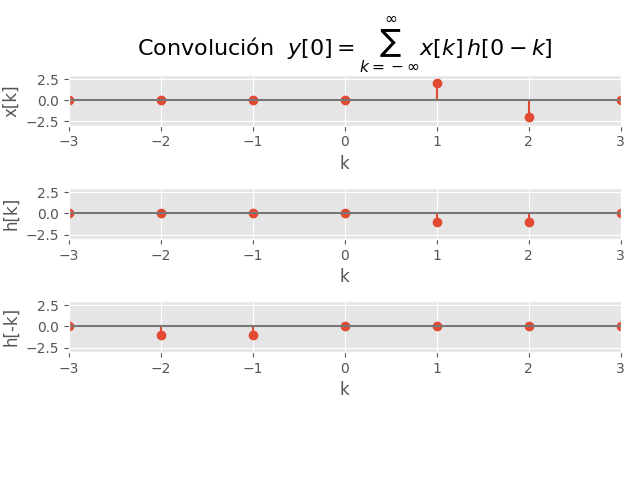
\includegraphics[width=6in]{./graphics/convejemp01-01.png}
    \caption{Se\~{n}ales $x[k]$, $h[k]$ y $h[-k]$.}
    \label{convejemp0101eps}
\end{figure}

\begin{figure}
	\centering
	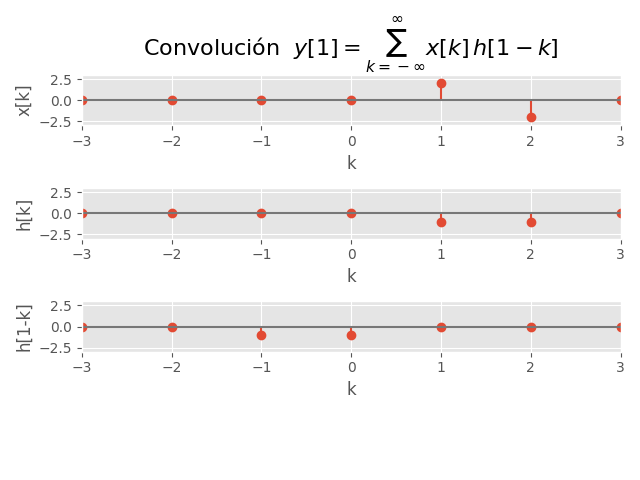
\includegraphics[width=6in]{./graphics/convejemp01-02.png}
    \caption{Se\~{n}ales $x[k]$, $h[k]$ y $h[1-k]$.}
	\label{convejemp0102eps}
\end{figure}

\begin{figure}
	\centering
	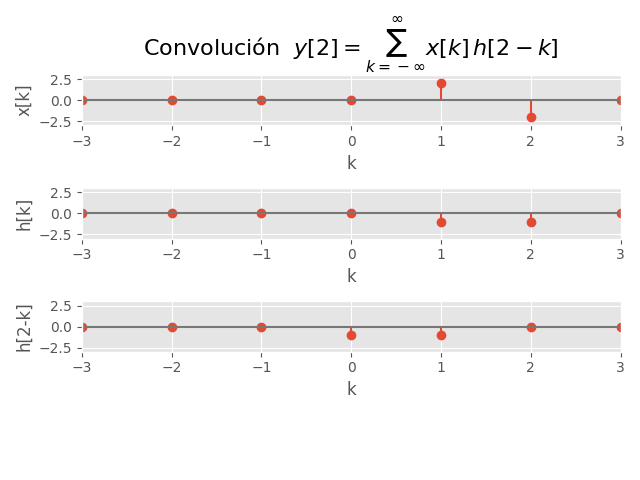
\includegraphics[width=6in]{./graphics/convejemp01-03.png}
    \caption{Se\~{n}ales $x[k]$, $h[k]$ y $h[2-k]$.}
	\label{convejemp0103eps}
\end{figure}

\begin{figure}
	\centering
	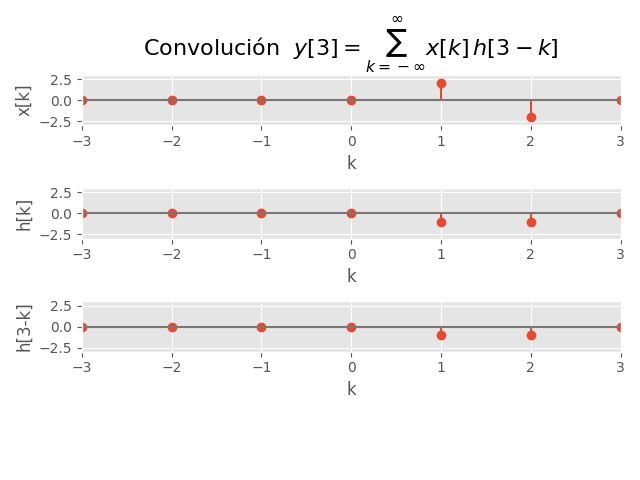
\includegraphics[width=6in]{./graphics/convejemp01-04.png}
    \caption{Se\~{n}ales $x[k]$, $h[k]$ y $h[3-k]$.}
	\label{convejemp0104eps}
\end{figure}

\begin{figure}
	\centering
	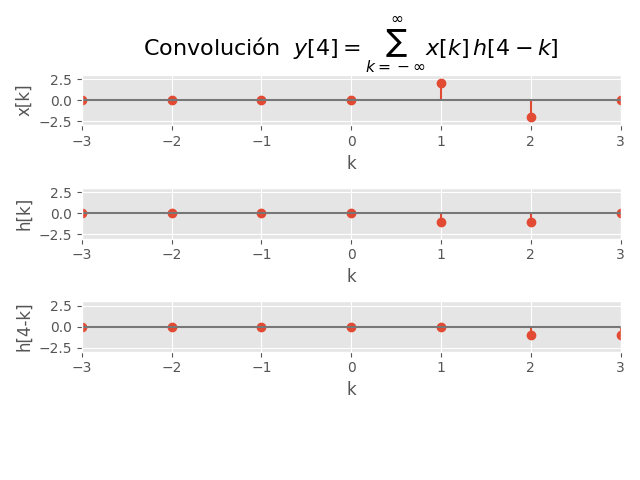
\includegraphics[width=6in]{./graphics/convejemp01-05.png}
    \caption{Se\~{n}ales $x[k]$, $h[k]$ y $h[4-k]$.}
	\label{convejemp0105eps}
\end{figure}

\begin{figure}
	\centering
	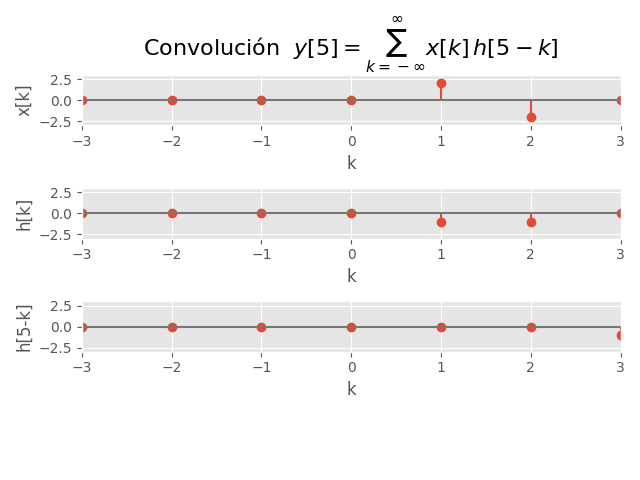
\includegraphics[width=6in]{./graphics/convejemp01-06.png}
    \caption{Se\~{n}ales $x[k]$, $h[k]$ y $h[5-k]$.}
	\label{convejemp0106eps}
\end{figure}


\subsection{Convoluci\'{o}n con un impulso}

Calculemos ahora la convoluci\'{o}n de las se\~{n}ales
\begin{eqnarray}
  x\left[ n\right] &=& \left( \frac{99}{100}\right) ^nu\left[ n\right] , \\
  h\left[ n\right] &=& \delta \left[ n-1\right] .
\end{eqnarray}

\subsubsection{Forma gr\'{a}fica}

\begin{enumerate}
\item Dibujemos las se\~{n}ales $x[k]$, $h[k]$ y $h[-k]$.
        
\item Dibujemos $h[n-k]$ para distintos valores de $n$, junto con
  $x[k]$. Ver (\ref{convejemp0201eps}).
        
\item Dibujemos el producto $z[n,k] = x[k] \, h[n-k]$.
        
\item Calculemos $\sum_{k}z[n,k]$ para obtener $y[n]$.
\end{enumerate}

\begin{figure}
	\centering
	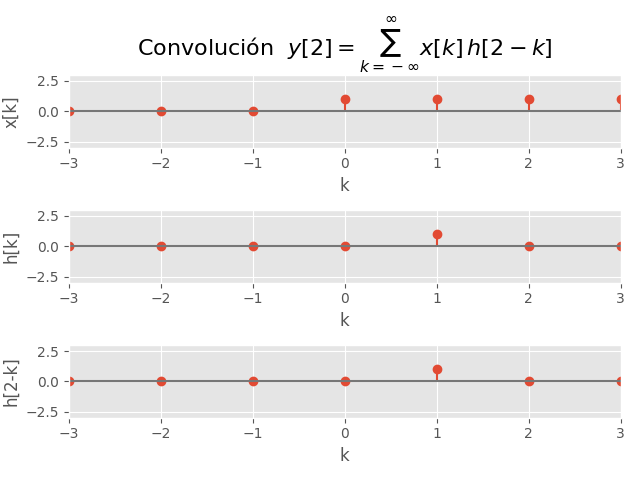
\includegraphics[width=6in]{./graphics/convejemp02-01.png}
    \caption{Se\~{n}ales $x[k]$, $h[k]$ y $h[2-k]$.}
	\label{convejemp0201eps}
\end{figure}

\subsubsection{Forma anal\'{\i}tica}

\begin{enumerate}
\item Seg\'{u}n la Ec. (\ref{convo}), tenemos
  \begin{equation}
    y\left[ n\right] =
    \sum_{k=-\infty }^{\infty }\left( \frac{99}{100}\right) ^{k}u \left[ k\right] \delta \left[ n-1-k\right].
  \end{equation}

\item Dado que dentro de la sumatoria aparece un escal\'{o}n unitario,
  podemos eliminarlo modificando adecuadamente el l\'{\i}mite inferior
  del \'{\i}ndice $k$.  Además, dado que la entrada contiene un factor escalón $u[n]$, la salida también tiene un factor similar. Entonces, 
  como $u[k] = 0$ para $k < 0$, el l\'{\i}mite
  inferior es $k = 0$, y además la sumatoria queda multiplicada por $u[n]$
  \begin{equation}
    y\left[ n\right] =\left(\sum_{k=0}^{\infty }\left( \frac{99}{100}\right) ^{k}\delta \left[ n-1-k\right]\right) \times u[n]. \label{ejeconvimpulso.0}
  \end{equation}

\item Observe que el \'{\i}ndice del impulso es $n - 1 - k$, y que por
  lo tanto est\'{a} ubicado en $k = n - 1$. Entonces
  \begin{equation}
    \sum_{k=0}^{\infty}\left( \frac{99}{100}\right) ^{k}\delta \left[ n-1-k\right] = 
    \left( \frac{99}{100}\right) ^{n-1}\delta \left[0\right] =
    \left( \frac{99}{100}\right) ^{n-1}
     \label{ejeconvimpulso}
  \end{equation}

\item Reemplazando (\ref{ejeconvimpulso}) en (\ref{ejeconvimpulso.0}), obtenemos
  \begin{equation}
  	y[n] = 
    \left( \frac{99}{100}\right) ^{n-1}
     \times u[n] .
  \end{equation}

\item En general, consideremos una respuesta al impulso
  \begin{equation}
    h\left[ n\right] = \delta \left[ n-n_{0}\right] .
  \end{equation}
  y calculemos su convoluci\'{o}n para una entrada gen\'{e}rica
  $x[n]$.

\item Seg\'{u}n la Ec. (\ref{convo}), tenemos
  \begin{equation}
    y\left[ n\right] =\sum_{k=-\infty }^{\infty } x[k] \, \delta \left[ n-n_{0}-k\right] ,
  \end{equation}

\item Observe que el \'{\i}ndice del impulso es $n - n_{0} - k$, y que
  por lo tanto est\'{a} ubicado en $k = n - n_{0}$. Entonces
  \begin{equation}
    x[k] \, \delta \left[ n-n_{0}-k\right] = x[n-n_{0}] \, \delta \left[0\right] = 
    x[n-n_{0}].
  \end{equation}

\item Considerando la sumatoria, obtenemos
  \begin{equation}
    \sum_{k=-\infty}^{\infty }x[n-n_{0}]\delta \left[ n-n_{0}-k\right] = 
    x[n-n_{0}] .
  \end{equation}

\item Dado que
  \begin{equation}
    u[n-n_{0}] = \left( \sum_{k=-\infty}^{\infty } \delta \left[ n-n_{0}-k\right] \right)
  \end{equation}
  la salida $y[n]$ es
  \begin{equation}
    y\left[ n\right] = x[n-n_{0}] \, u[n-n_{0}].
  \end{equation}
\end{enumerate}

\subsection{Convoluci\'{o}n de una se\~{n}al con una ventana
  rectangular}

Calculemos la convoluci\'{o}n de las se\~{n}ales
\begin{eqnarray}
  x\left[ n\right] &=&\left( \frac{1}{2}\right) ^nu\left[ n\right] ,                                      \\
  h\left[ n\right] &=&u\left[ n\right] -u\left[ n-2\right] =
  \delta \left[ n \right] +\delta \left[ n-1\right] ,
\end{eqnarray}

\subsubsection{Forma gr\'{a}fica}

\begin{enumerate}
\item Dibujemos las se\~{n}ales $x[k]$, $h[k]$ y $h[-k]$.
        
\item Dibujemos $h[n-k]$ para distintos valores de $n$, junto con
  $x[k]$.
        
\item Dibujemos el producto $z[n,k] = x[k] h[n-k]$.
        
\item Calculemos $\sum_{k}z[n,k]$ para obtener $y[n]$.
\end{enumerate}

\subsubsection{Forma anal\'{\i}tica}

% rehacer figura convo

\begin{enumerate}
\item Seg\'{u}n la Ec. (\ref{convo}), tenemos
  \begin{equation}
    y\left[ n\right] =
    \sum_{k=-\infty }^{\infty }\left( \frac{1}{2}\right) ^{k} \,
    u\left[ k\right] \, h\left[ n-k\right].
  \end{equation}

\item Ajustamos los \'{\i}ndices de la sumatoria porque la ventana
  rectangular es nula para $k < 0$
  \begin{equation}
    y\left[ n\right] =
    \sum_{k=0}^{\infty }\left( \frac{1}{2}\right) ^{k} \, h\left[n-k\right].
  \end{equation}
        
\item Expresamos a la ventana rectangular como una suma de impulsos
  desplazados en el tiempo
  \begin{equation}
    y\left[ n\right] =
    \sum_{k=0}^{\infty }
    \left( \frac{1}{2}\right) ^{k}\left(\delta \left[ n-k\right] +\delta \left[ n-1-k\right] \right).
  \end{equation}
        
\item Desdoblamos la convoluci\'{o}n en dos,
  \begin{eqnarray}
    \sum_{k=0}^{\infty }\left( \frac{1}{2}\right) ^{k} \, \delta \left[ n-k\right]
    &=&\left( \frac{1}{2}\right) ^n u[n], \\
    \sum_{k=0}^{\infty }\left( \frac{1}{2}\right) ^{k} \, \delta \left[ n-1-k\right]
    &=&\left( \frac{1}{2}\right) ^{n-1} u[n-1].
  \end{eqnarray}
        
\item El resultado final es
  \begin{equation}
    y\left[ n\right] =\left( \frac{1}{2}\right)^n \, u[n] +\left(
      \frac{1}{2}\right)^{n-1} \, u[n-1].
  \end{equation}
\end{enumerate}

\subsection{Convoluci\'{o}n de se\~{n}ales infinitas}

Considere una entrada $x\left[ n\right] $ y una respuesta al impulso
unitario dadas por
\begin{eqnarray}
  x\left[ n\right] &=&\alpha ^nu\left[ n\right] , \\
  h\left[ n\right] &=&u\left[ n\right] ,
\end{eqnarray}
donde el valor absoluto de $\alpha$ es menor que $1$, 
\begin{equation}
0< | \alpha | <1.
\end{equation}

\subsubsection{Forma gr\'{a}fica}

\begin{enumerate}
\item Dibujemos las se\~{n}ales $x[k]$, $h[k]$ y $h[-k]$.
        
\item Dibujemos $h[n-k]$ para distintos valores de $n$, junto con
  $x[k]$.
        
\item Dibujemos el producto $z[n,k] = x[k] \, h[n-k]$.
        
\item Calculemos $\sum_{k} z[n,k]$ para obtener una aproximaci\'{o}n de
  $y[n]$
\end{enumerate}

\subsubsection{Forma anal\'{\i}tica}

\begin{enumerate}
\item Seg\'{u}n la Ec. (\ref{convo}), tenemos
  \begin{equation}
    \alpha^{k} u[k] u[n-k] =
    \left\{ \begin{array}{ll}
        \alpha ^{k}, & 0\leq k\leq n, \\ 
        0, & \left( k<0\right) \vee \left( k>n\right)
      \end{array} \right.             \label{convinf}
  \end{equation}

\item Para poder realizar esta sumatoria, debemos recordar sucesiones
  geométricas.  Definamos la suma parcial
  \begin{equation}
    S_{n}=    \sum_{k=0}^n\alpha ^{k},
  \end{equation}
  y multipliquemos por $a$ para obtener
  \begin{equation}
    \alpha \, S_{n}=   \sum_{k=0}^n\alpha ^{k+1}.
  \end{equation}
  Entonces podemos escribir
  \begin{equation}
    S_{n}-\alpha \, S_{n}= \left( \sum_{k=0}^n\alpha ^{k}\right) - \left( \sum_{k=0}^n\alpha ^{k+1}\right)
  \end{equation}
  y simplificando
  \begin{equation}
    S_n- \alpha \, S_n=\alpha^{0}-\alpha^{n+1}.
  \end{equation}
  Podemos despejar entonces
  \begin{equation}
    S_n=\frac{\alpha^{0}-\alpha^{n+1}}{1-\alpha}=\frac{1-\alpha^{n+1}}{1-\alpha}.    \label{sumageo}
  \end{equation}

\item Aplicamos la Ec. (\ref{sumageo}) a la Ec. (\ref{convinf})
  \begin{equation}
    \sum_{k=0}^n\alpha ^{k}=\frac{1-\alpha ^{n+1}}{1-\alpha }.      \label{sumaserie}
  \end{equation}
  Por lo tanto, la respuesta es
  \begin{equation}
    y\left[ n\right] =\left( \frac{1-\alpha ^{n+1}}{1-\alpha }\right) u\left(n\right) .
  \end{equation}
\end{enumerate}

\subsection{Convoluci\'{o}n de una se\~{n}al consigo misma}

Vamos a calcular la convolución de una señal consigo misma, definiendo
\begin{eqnarray}
  x\left[ n\right] =\left( \frac{8}{10}\right)^n u\left[ n\right] ,       \\
  h\left[ n\right] =\left( \frac{8}{10}\right)^n u\left[ n\right] .
\end{eqnarray}

\subsubsection{Forma gr\'{a}fica}

\begin{enumerate}
\item Dibujemos las se\~{n}ales $x[k]$, $h[k]$ y $h[-k]$.
        
\item Dibujemos $h[n-k]$ para distintos valores de $n$, junto con
  $x[k]$.
        
\item Dibujemos el producto $z[n,k] = x[k] h[n-k]$.
        
\item Calculemos $\sum_{k}z[n,k]$ para obtener $y[n]$ en forma
  aproximada
\end{enumerate}

\subsubsection{Forma anal\'{\i}tica}

\begin{enumerate}
\item Seg\'{u}n la Ec. (\ref{convo}), tenemos
  \begin{equation}
    y\left[ n\right] =
    \sum_{k=-\infty }^{\infty }
    \left( \frac{8}{10}\right)^{k} u\left[ k\right] 
    \left( \frac{8}{10}\right)^{n-k} u\left[ n-k\right] ,
  \end{equation}

\item Podemos modificar los l\'{\i}mites de la sumatoria, pues $u[k] =
  $ para $k < 0$, y $u[n-k] = 0$ para $n - k < 0$
  \begin{equation}
    y\left[ n\right] = (\sum_{k=0}^{n }\left( \frac{8}{10}\right) ^{k+n-k}) \times u[n].
  \end{equation}
   Observe que si uno de los factores de la entrada es un escalón $u[n - n_{0}]$, la salida también tiene el mismo factor.
   
\item Extraemos de la sumatoria el factor com\'{u}n de todos los
  sumandos $(\frac{8}{10})^{n}$, que es independiente de $k$, y obtenemos
  \begin{equation}
    y\left[ n\right] = \left(\left( \frac{8}{10}\right) ^{n} \sum_{k=0}^{n} 1\right) \times u[n],
  \end{equation}

\item Finalmente resulta esto
  \begin{equation}
    y\left[ n\right] = \left( \frac{8}{10}\right) ^{n} \, \left(n+1
    \right) \, u[n].
  \end{equation}
  El factor $u[n]$ aparece porque la sumatoria cuyo resultado es $n +
  1$ tiene un l\'{\i}mite inferior $k = 0$, y por lo tanto la sumatoria es no nula sí y solo sí $n \geq 0$.
\end{enumerate}
 % Suma de convoluci\'{o}n

\chapter{Sistemas LIT y la convolución}

\section{Introducci\'{o}n}

Hemos visto que la suma de convoluci\'{o}n 
\begin{equation}
    y\left[ n\right] =
     \sum_{k=-\infty }^{\infty }x\left[ k\right] \, h\left[ n-k\right] = x\left[ n\right] * h\left[ n\right] ,
\end{equation}
define la respuesta $y$ de un sistema $LIT$ para una entrada $x$ si conocemos la respuesta al 
impulso $h$. Por lo tanto, en este cap\'{\i}tulo usaremos la convoluci\'{o}n como herramienta para 
estudiar distintas propiedades de los sistemas LIT.

\section{Propiedades de los sistemas LIT}

\subsection{La propiedad conmutativa}

El resultado de la convoluci\'{o}n es independiente del ordenamiento de las se\~{n}ales, o en otras 
palabras, un sistema LIT de respuesta al impulso $h$ excitado con una entrada $x$ genera una salida 
similar al de un sistema LIT de respuesta al impulso $x$ excitado con una entrada $h$.

Consideremos la operaci\'{o}n de convoluci\'{o}n
\begin{equation}
y\left[ n\right] =
        \sum_{k=-\infty }^{\infty }x\left[ k\right] \, h\left[ n-k\right] =
        \sum_{k=-\infty }^{\infty }h\left[ k\right] \, x\left[ n-k\right].
\end{equation}

Realizamos un cambio de variable $m=n-k$ y por consecuencia definimos $k=m-n$ para obtener
\begin{equation}
        y\left[ n\right] =
                \sum_{k=-\infty }^{\infty }x\left[ k\right] \, h\left[ n-k\right] =
                \sum_{m=-\infty }^{\infty }x\left[ n-m\right] \, h\left[ m\right].
\end{equation}

\subsection{La propiedad distributiva}

La salida de un sistema LIT cuya respuesta al impulso es $h_{a} + h_{b}$ para una entrada $x$ es 
similar a la suma de las salidas de dos sistemas de respuestas al impulso $h_{a}$ y $h_{b}$ frente a una 
entrada $x$.

Probaremos la distributividad de la convoluci\'{o}n discreta
\begin{eqnarray}
       y\left[ n\right] &=&x\left[ n\right]  * \left( h_{a}\left[ n\right] + h_{b}\left[ n\right] \right) , \\
       y\left[ n\right] &=&x\left[ n\right]  * h_{a}\left[ n\right] + x\left[ n\right]  * h_{b}\left[ n\right],
\end{eqnarray}
planteando
\begin{equation}
 y\left[ n\right] =
\sum_{k=-\infty }^{\infty }x\left[ k\right] \, \left( h_{a}\left[ n-k\right] +h_{b}\left[ n-k\right] \right).
\end{equation}
Dado que la multiplicaci\'{o}n es distributiva respecto a la suma, obtenemos
\begin{equation}
        y\left[ n\right] =
        \sum_{k=-\infty }^{\infty }
        \left( x\left[ k\right] \, h_{a}\left[ n-k\right] +x\left[ k\right] \,h_{b}\left[ n-k\right] \right).
\end{equation}
Reagrupando t\'{e}rminos
\begin{equation}
        y\left[ n\right] =
                \sum_{k=-\infty }^{\infty }
                        \left(  \left( 
                                        x\left[ k\right] \, h_a\left[ n-k\right] 
                                \right) +
                                \left( 
                                        x\left[ k\right] \, h_{b}\left[ n-k\right] 
                                \right) 
                        \right) ,
\end{equation}
y separando sumatorias
\begin{equation}
        y\left[ n\right] =
                \sum_{k=-\infty }^{\infty }\left( x\left[ k\right] \, h_{a}\left[ n-k\right] \right) +
                \sum_{k=-\infty }^{\infty }\left( x\left[ k\right] \, h_{b}\left[ n-k\right] \right) ,
\end{equation}
obtenemos
\begin{equation}
y\left[ n\right] =x\left[ n\right]  * h_a\left[ n\right] +x\left[ n \right] * h_{b}\left[ n\right] .
\end{equation}

\subsection{La propiedad asociativa}

La operaci\'{o}n de convoluci\'{o}n es asociativa
\begin{eqnarray}
y\left[ n\right] &=&x\left[ n\right] * \left( h_a\left[ n\right] * h_{b} \left[ n\right] \right) , \\
y\left[ n\right] &=&\left( x\left[ n\right] *h_a\left[ n\right] \right) * h_{b}\left[ n\right] , \\
y\left[ n\right] &=&x\left[ n\right] *h_a\left[ n\right] *h_{b}\left[ n\right].
\end{eqnarray}

Para probar la propiedad asociativa, planteamos las dos formas de hacer el cálculo.
Primero consideremos
\begin{equation}
 y_{1}[n] = \sum_{p=-\infty}^{\infty} x[p] \, h_{a}[n-p],
\end{equation}
\begin{equation}
 y[n] = \sum_{q=-\infty}^{\infty} y_{1}[q] \, h_{b}[n-q].
\end{equation}
\begin{equation}
 y[n] = \sum_{q=-\infty}^{\infty} \left( \sum_{p=-\infty}^{\infty} x[p] \, h_{a}[q-p] \right) \, h_{b}[n-q].
\end{equation}
y
\begin{equation}
 y[n] = \sum_{q=-\infty}^{\infty} \sum_{p=-\infty}^{\infty} x[p] \, h_{a}[q-p]  \, h_{b}[n-q].
\end{equation}
Despues consideramos el cálculo alternativo
\begin{equation}
       h[n] = \sum_{r=-\infty}^{\infty} h_{a}[r] \, h_{b}[n-r],
\end{equation}
\begin{equation}
      y[n] = \sum_{s=-\infty}^{\infty} x[s] \, h[n-s],
\end{equation}
\begin{equation}
      y[n] = \sum_{s=-\infty}^{\infty} x[s] \, \left( \sum_{r=-\infty}^{\infty} h_{a}[r] \, h_{b}[n - r - s] \right),
\end{equation}
y
\begin{equation}
      y[n] = \sum_{s=-\infty}^{\infty} \sum_{r=-\infty}^{\infty} x[s] \, h_{a}[r] \, h_{b}[n -r -s].
\end{equation}
Por lo tanto, comparemos
\begin{equation}
 y[n] = \sum_{q=-\infty}^{\infty} \sum_{p=-\infty}^{\infty} x[p] \, h_{a}[q-p]  \, h_{b}[n-q],
\end{equation}
\begin{equation}
 y[n] = \sum_{s=-\infty}^{\infty} \sum_{r=-\infty}^{\infty} x[s] \, h_{a}[r] \, h_{b}[n -r -s].
\end{equation}
Considerando las igualdades
\begin{equation}
 p = s, \qquad q - p = r,
\end{equation}
obtenemos
\begin{equation}
 n - q = n - q + p - p = n - r - s, 
\end{equation}
y por lo tanto
\begin{equation}
\begin{array}{c}
 \sum_{s=-\infty}^{\infty} \sum_{r=-\infty}^{\infty} x[s] \, h_{a}[r] \, h_{b}[n -r -s] = \\
 \\ 
 \sum_{q=-\infty}^{\infty} \sum_{p=-\infty}^{\infty} x[p] \, h_{a}[q - p] \, h_{b}[n -q].
\end{array}
\end{equation}


\subsection{Preguntas}

\begin{enumerate}
\item ¿Qu\'{e} significado tiene la propiedad conmutativa de los sistemas lineales?
\item ¿Qu\'{e} significado tiene la propiedad distributiva de los sistemas lineales?
\item ¿Qu\'{e} significado tiene la propiedad asociativa de los sistemas lineales?
\item D\'{e} alg\'{u}n ejemplo concreto de estas tres propiedades.
\end{enumerate}

\subsection{Sistemas LIT con y sin memoria}

Un sistema no tiene memoria si su salida en cualquier momento depende solamente de la entrada de ese momento.

Si un sistema no tiene memoria entonces debe ser $h\left[ n\right]=0$, 
para todo $n\neq 0$, y por lo tanto 
\begin{equation}
h\left[ n\right] = K \, \delta \left[ n\right] .
\end{equation}
Si un sistema tiene una respuesta al impulso $h\left[ n\right] $ que es distinta de $0$ para $n\neq 0,$ entonces el sistema tiene memoria.

\subsection{Preguntas}

\begin{enumerate}
\item ¿Conoce alg\'{u}n sistema f\'{\i}sico que no tenga memoria?
\item ¿Conoce alg\'{u}n sistema f\'{\i}sico que tenga memoria?
\end{enumerate}

\subsection{Sistemas LIT causales}

Si $y\left[n_{0}\right] $ no depende de $x\left[ n\right] $ para $n>n_{0},$ entonces un sistema LIT es causal. 
Entonces todos los valores $h\left[n\right]$  para $n<0$ deben ser $0$ y por lo tanto en
la suma de convoluci\'{o}n podemos cambiar el límite superior 
\begin{equation}
y\left[n\right] =\sum_{k=-\infty}^{n}x\left[k\right] \, h\left[ n-k\right],
\end{equation}
porque debe ser $n - k \geq 0$, o $n \geq k$.

Además, si la entrada $x[n]$ comienza en $n = 0$, podemos cambiar el límite inferior de la sumatoria
\begin{equation}
	y\left[n\right] =\sum_{k=0}^{n}x\left[k\right] \, h\left[ n-k\right].
\end{equation}
Esta fórmula significa que podemos calcular la salida de un sistema LIT de tiempo discreto con una cantidad limitada de multiplicaciones y sumas.


\subsection{Preguntas}

Indicar si las siguientes afirmaciones son verdaderas o falsas, en el caso de un sistema lineal invariante en el tiempo:

\begin{enumerate}
\item  Si la entrada es nula para todo tiempo, entonces la salida es nula para todo tiempo.

\item  Si la relaci\'{o}n entre entrada y salida es 
$y[n] =x[n] \, \cos \left(n\right) ,$ entonces el sistema  es LIT.

\item  Si la relaci\'{o}n entre entrada y salida es 
$y[n] =\sum_{k=0}^{n} x[k] ,$ entonces el sistema es LIT. 
\end{enumerate}

\subsection{Sistemas LIT estables e inestables}

\subsubsection{Estabilidad BIBO}

El criterio de estabilidad \textbf{B}ounded \textbf{I}nput \textbf{B}ounded \textbf{O}utput 
(entrada acotada, salida acotada) se puede expresar matem\'{a}ticamente como 
\begin{equation}
        \left| x\left[ n\right] \right| < M_{x} \rightarrow \left| y\left[ n\right]\right| < M_{y},
\end{equation}
para tiempo discreto, o 
\begin{equation}
        \left| x\left( t\right) \right| < M_{x} \rightarrow \left| y\left( t\right)\right| < M_{y},
\end{equation}
para tiempo continuo.

El sistema es estable si para entradas acotadas 
\begin{equation}
        \left| x\left[ k\right] \right| <M_{x},
\end{equation}
tenemos salidas acotadas 
\begin{equation}
        \left| y\left[ k\right] \right| <M_{y}.
\end{equation}
La suma de convoluci\'{o}n es 
\begin{equation}
        y\left[ n\right] =\sum_{k=0}^nx\left[ k\right] \, h\left[ n-k\right] .
\end{equation}
Entonces podemos escribir 
\begin{equation}
        \left| y\left[ n\right] \right| =
                \left| 
                        \sum_{k=0}^nx\left[ k\right] \, h\left[ n-k\right] 
                \right| \leq 
                \sum_{k=0}^n\left| x\left[ k\right] \right| \, \left| h\left[ n-k\right] \right| ,
\end{equation}
y aplicando la desigualdad triangular obtenemos la cota para $|y[n]|$
\begin{equation}
        \left| y\left[ n\right] \right| 
        \leq 
        \sum_{k=0}^n
                \left| x\left[ k\right]\right| \,
                \left| h\left[ n-k\right] \right| 
        \leq 
        \left( 
                \sum_{k=0}^n\left| x\left[ k\right] \right| 
        \right) \,
        \left( \sum_{k=0}^n\left| h\left[ n-k\right] \right| \right) .
\end{equation}
Dado que resulta
\begin{equation}
        \left| y\left[ n\right] \right| \leq 
        M_{x} \, \left( \sum_{k=0}^n\left| h\left[n-k\right] \right| \right) \leq M_{y}.
\end{equation}
Dado que $M_{y}$ es finito entonces el valor absoluto de la respuesta al impulso es acotada.


\subsection{Respuesta de un sistema LIT en tiempo discreto a una entrada exponencial imaginaria}

\begin{enumerate}
	\item Vamos a calcular la convolución de una entrada $x[n] = e^{j \, \omega \, n}$ con una respuesta al impulso $h[n]$. 
	
	\item Comenzamos escribiendo la fórmula de la suma de convolución
	\begin{equation}
		y\left[ n\right] =
		\sum_{k=-\infty }^{\infty }x\left[ k\right] \, h\left[ n-k\right] =
		\sum_{k=-\infty }^{\infty }h\left[ k\right] \, x\left[ n-k\right].
	\end{equation}

    \item Vamos a usar la fórmula alternativa
	\begin{equation}
	y\left[ n\right] =
	\sum_{k=-\infty }^{\infty }h\left[ k\right] \, x\left[ n-k\right].
    \end{equation}

    \item Sustituyendo $x[n - k] =  e^{j \, \omega \, (n-k)}$ obtengo
     \begin{equation}
	    y\left[ n\right] =
	    \sum_{k=-\infty }^{\infty }h\left[ k\right] \, e^{j \, \omega \, (n-k)} =
	    \sum_{k=-\infty }^{\infty }h\left[ k\right] \, e^{-j \, \omega \, k} \, e^{j \, \omega \, n}. \label{dt.eigenfunc.1}
     \end{equation}
   
     \item Viendo la ecuación (\ref{dt.eigenfunc.1}) podemos extraer el factor común $e^{j \, \omega \, n}$ de la sumatoria y escribir
     \begin{equation}
	y\left[ n\right] =
	\left(\sum_{k=-\infty }^{\infty }h\left[ k\right] \, e^{-j \, \omega \, k}\right) \, e^{j \, \omega \, n}. \label{dt.eigenfunc.2}
    \end{equation}

    \item Viendo la ecuación (\ref{dt.eigenfunc.2}), podemos definir $H(e^{j \, \omega})$, la transformada de Fourier de $h[n]$
    \begin{equation}
	H(e^{j \, \omega}) =
	\sum_{k=-\infty }^{\infty }h\left[ k\right] \, e^{-j \, \omega \, k}. \label{dt.eigenfunc.3}
    \end{equation}	 

    \item Entonces resulta
    \begin{equation}
    	y[n] = H(e^{j \, \omega}) \, e^{j \, \omega \, n}.
    \end{equation}
    Se dice que las funciones de la forma $e^{j \, \omega \, n}$ son autofunciones de los sistemas lineales invariantes en el tiempo.
\end{enumerate}  

\subsection{Respuestas}

Estas son las respuestas a las preguntas planteadas arriba

\begin{enumerate}
	\item ¿Qu\'{e} significado tiene la propiedad conmutativa de los sistemas lineales?
	Un sistema LIT con respuesta al impulso $h[n]$ responde a una entrada $x[n]$ igual que un sistema LIT con respuesta al impulso $x[n]$ responde a una entrada $h[n]$. Además, cuando conectamos en serie dos sistemas LIT, no importa el orden en que se conecten: el conjunto de los dos sistemas va a responder igual ante cualquier entrada.
	
	\item ¿Qu\'{e} significado tiene la propiedad distributiva de los sistemas lineales?
	Podemos implementar un sistema LIT con respuesta al impulso $h_{1}[n] + h_{2}[n]$ conectando en paralelo dos sistemas LIT cuyas respectivas respuestas al impulso sean $h_{1}[n]$ y $h_{2}[n]$.
	
	\item ¿Qu\'{e} significado tiene la propiedad asociativa de los sistemas lineales?
	Cuando conectamos en serie sistemas LIT, podemos formar nuevos sistemas LIT.
	
	\item ¿Conoce alg\'{u}n sistema f\'{\i}sico que no tenga memoria? Un cable.
	\item ¿Conoce alg\'{u}n sistema f\'{\i}sico que tenga memoria? Un tanque de agua (acumula o "recuerda" el agua que entra).

    \item  ¿La siguiente afirmación es verdadera o falsa? 
    "Si la entrada es nula para todo tiempo, entonces la salida es nula para todo tiempo."
    \textbf{Verdadero, pues si la entrada es nula, la suma de convoluci\'{o}n es nula.}

   \item  ¿La siguiente afirmación es verdadera o falsa? "Si la relaci\'{o}n entre entrada y salida es 
   $y[n] =x[n] \, \cos \left(n\right) ,$ entonces el sistema  es LIT." 
    \textbf{Falso, porque la respuesta al impulso depende del tiempo en que el impulso ocurre.}
    \begin{equation}
                y[n] = \delta[n - n_{0}] \, \cos \left( n_{0} \right).
    \end{equation}

\item  ¿La siguiente afirmación es verdadera o falsa? Si la relaci\'{o}n entre entrada y salida es 
$y[n] =\sum_{k=0}^{n} x[k] ,$ entonces el sistema es LIT. 
    \textbf{Verdadero, pues dicha relaci\'{o}n puede escribirse como una convoluci\'{o}n} 
        \begin{equation}
                y[n] = \sum_{k=-\infty}{\infty} x[k] \, u[k] \, u[n-k].
        \end{equation}
\end{enumerate}
 % Propiedades de sistemas LIT y la suma de convoluci\'{o}n

\chapter{La integral de convolución}

\section{Deducci\'{o}n de la f\'{o}rmula}

A continuaci\'{o}n calculamos la salida $y(t)$ para una entrada arbitraria $x(t)$ en función de la respuesta al impulso $h(t)$ del sistema lineal invariante en el tiempo.

\subsection{Una se\~{n}al como l\'{\i}mite de una sumatoria}

\begin{figure}
	\centering
	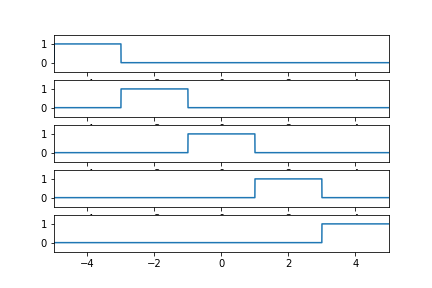
\includegraphics[width=0.7\linewidth]{graphics/pulses}
	\caption{Pulsos desplazados en el tiempo}
	\label{fig:pulses}
\end{figure}

\begin{figure}
	\centering
	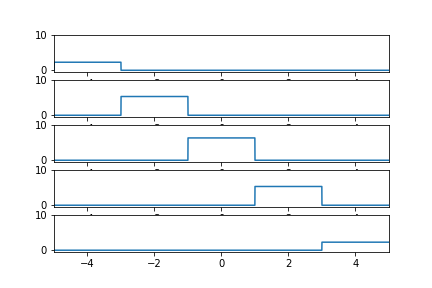
\includegraphics[width=0.7\linewidth]{graphics/modulated_pulses}
	\caption{Pulsos desplazados en el tiempo y modulados}
	\label{fig:modulatedpulses}
\end{figure}

\begin{figure}
	\centering
	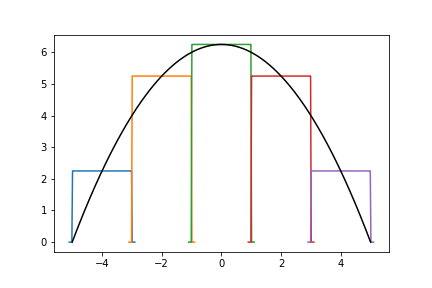
\includegraphics[width=0.7\linewidth]{graphics/coarse-approximation}
	\caption{Aproximación grosera}
	\label{fig:coarse-approximation}
\end{figure}

\begin{figure}
	\centering
	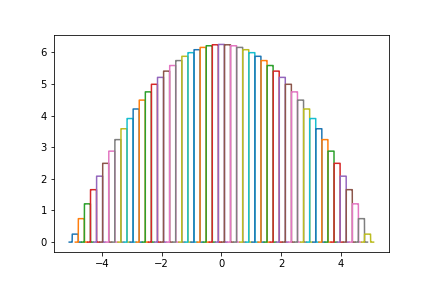
\includegraphics[width=0.7\linewidth]{graphics/fine-approximation}
	\caption{Aproximación fina}
	\label{fig:fine-approximation}
\end{figure}

Vamos a probar que podemos representar una se\~{n}al 
continua como el l\'{\i}mite de una suma de pulsos.
Consideremos pulsos desplazados en el tiempo $\delta _{\Delta }\left(t-k \, \Delta \right)$ 
donde $\Delta$ es un incremento de tiempo variable. 
Observando la figura \ref{fig:pulses}, podemos escribir las definiciones de los pulsos desplazados en el tiempo
\begin{equation}
        \begin{array}{c}
                ...                                             \\ 
                \delta _{\Delta }\left( t+\Delta \right) =
                        \left\{ \begin{array}{l}
                                        \frac{1}{\Delta },      \\ 
                                        0,
                                \end{array}
                                \begin{array}{l}
                                        -\Delta \leq t<0,       \\ 
                                        \left( t<-\Delta \right) \vee \left( 0\leq t\right) ,
                                \end{array}
                        \right.                                 \\ 
                \delta _{\Delta }\left( t\right) =
                        \left\{ \begin{array}{l}
                                        \frac{1}{\Delta },      \\ 
                                        0,
                                \end{array}
                                \begin{array}{l}
                                        0\leq t<\Delta ,        \\ 
                                        \left( t<0\right) \vee \left( \Delta \leq t\right) ,
                                \end{array}
                        \right.                                 \\ 
                \delta _{\Delta }\left( t-\Delta \right) =
                        \left\{ \begin{array}{l}
                                        \frac{1}{\Delta },      \\ 
                                        0,
                                \end{array}
                                \begin{array}{l}
                                        \Delta \leq t<2 \, \Delta , \\ 
                                        \left( t<\Delta \right) \vee \left( 2 \, \Delta \leq t\right) ,
                                \end{array}
                        \right.                                 \\ 
                ...                                             \\ 
                \delta _{\Delta }\left( t-k \, \Delta \right) =
                        \left\{ \begin{array}{l}
                                        \frac{1}{\Delta },      \\ 
                                        0,
                                \end{array}
                         \begin{array}{l}
                            k \, \Delta \leq t<\left( k+1\right) \, \Delta , \\ 
                              \left( t<k \, \Delta \right) \vee \left( \left( k+1\right) \, \Delta \leq t\right) .
                         \end{array}
               \right.
        \end{array}
\end{equation}
Multiplicando por $x\left( k \, \Delta \right) \, \Delta $ al $k-\acute{e}simo$ pulso (ver figura \ref{fig:modulatedpulses}) se obtiene 
\begin{equation}
        \begin{array}{c}
                        ...                                                                    \\ 
                        x\left( -\Delta \right) \, \delta _{\Delta }\left( t+\Delta \right) \, \Delta =
                                \left\{ \begin{array}{l}
                                                \frac{x\left( -\Delta \right) }{\Delta } \, \Delta ,        \\ 
                                                0,
                                        \end{array}
                                        \begin{array}{l}
                                           -\Delta \leq t<0,                                       \\ 
                                          \left( t<-\Delta \right) \vee \left( 0\leq t\right) ,
                                        \end{array}
                                \right.                                                                 \\ 
                        x\left( 0\right) \, \delta _{\Delta }\left( t\right) \, \Delta =
                                \left\{ \begin{array}{l}
                                                \frac{x\left( 0\right) }{\Delta } \, \Delta ,               \\ 
                                                0,
                                        \end{array}
                                        \begin{array}{l}
                                                0\leq t<\Delta ,                                        \\ 
                                                \left( t<0\right) \vee \left( \Delta \leq t\right) ,
                                        \end{array}
                                \right.                                                                 \\ 
                        x\left( \Delta \right) \, \delta _{\Delta }\left( t-\Delta \right) \, \Delta =
                                \left\{ \begin{array}{l}
                                                \frac{x\left( \Delta \right) }{\Delta } \, \Delta ,         \\ 
                                                0,
                                        \end{array}
                                        \begin{array}{l}
                                                \Delta \leq t<2 \, \Delta ,                                 \\ 
                                                \left( t<\Delta \right) \vee \left( 2 \, \Delta \leq t\right) ,
                                        \end{array}
                                \right.                                                                 \\ 
                        ... \\ 
                        x\left( k\Delta \right) \, \delta _{\Delta }\left( t-k\Delta \right) \, \Delta =
                                \left\{ \begin{array}{l}
                                                \frac{x\left( k \, \Delta \right) }{\Delta } \, \Delta ,        \\ 
                                                0,
                                        \end{array}
                       \begin{array}{l}
                             k \, \Delta \leq t<\left( k+1\right) \, \Delta ,               \\ 
                             \left( t<k \, \Delta \right) \vee \left( \left( k+1\right) \, \Delta \leq t\right) .
                       \end{array}
                       \right.
        \end{array}
\end{equation}
Observe que un valor dado de $t$ (por ejemplo $t_{0})$ s\'{o}lo puede pertenecer a \textbf{un} intervalo 
$k\Delta \leq t<\left( k+1\right) \Delta,$ por lo tanto para $t_{0}$ solo uno de los productos puede ser 
distinto de $0$. Sumando los infinitos productos (ver figura \ref{fig:coarse-approximation}) obtenemos 
\begin{equation}
   x_{\Delta }\left( t\right) =
     \sum_{k=-\infty }^{\infty }x\left( k\Delta \right) \, \delta _{\Delta }\left( t-k \, \Delta \right) \, \Delta .
\end{equation}

%\begin{figure*}[ht]
%\begin{center}
%\includegraphics[scale=.70]{./graphics/contcont222.eps}
%\end{center}
%\caption{Se\~{n}ales como suma de pulsos}
%\label{contcont222eps}
%\end{figure*}

Considerando la suma de los pulsos desplazados en el tiempo 
podemos observar que cuando $\Delta $ tiende a cero (ver figura \ref{fig:fine-approximation}) $x_{\Delta }\left( t\right) $ tiende a $x\left( t\right).$
\begin{equation}
        x\left( t\right) =      
\begin{array}{l}
    Lim \\ 
    \Delta \rightarrow 0
\end{array}
x_{\Delta }\left( t\right) = 
\begin{array}{l}
    Lim \\ 
    \Delta \rightarrow 0
\end{array}
   \sum_{k=-\infty }^{\infty }x\left( k \, \Delta \right) \, \delta _{\Delta }\left(t-k \, \Delta \right) \, \Delta .
\end{equation}
Adem\'{a}s, cuando $\Delta $ tiende a cero, la sumatoria se convierte en una integral 
\begin{equation}
        x\left( t\right) =\int_{-\infty }^{\infty }x\left( \tau \right) \, \delta\left( t-\tau \right) \, d\tau .
        \label{integral.convolucion}
\end{equation}

Notemos que por la propiedad del muestreo, debe cumplirse 
\begin{equation} 
     x\left( t\right) \, \delta \left( t-\tau \right) =
   x\left( \tau \right) \, \delta \left( t-\tau \right),
\end{equation}
y en ese caso 
\begin{equation}
 x\left( t\right) = 
  x\left( t\right) \, \left( \int_{-\infty }^{\infty } \delta \left( t-\tau \right) \, d\tau \right) .
\end{equation}

\subsection{La respuesta al impulso y la convolución}

Definamos $h_{k \, \Delta }(t) = h_{\Delta }\left( t-k \, \Delta \right)$ como la salida de un sistema invariante en el tiempo para el pulso 
$\delta _{\Delta }(t-k \, \Delta ).$ 

Además, recordemos la ecuaci\'{o}n (\ref{integral.convolucion})
\begin{equation}
 x_{\Delta }\left( t\right) =
  \sum_{k=-\infty }^{\infty }x\left( k \, \Delta \right) \, \delta _{\Delta }\left( t-k \, \Delta \right) \, \Delta ,
\end{equation}

La salida $y_{\Delta }\left( t\right) $ para una entrada $x_{\Delta }\left( t\right) $ puede 
definirse, por el principio de superposici\'{o}n, como 
\begin{equation}
        y_{\Delta }\left( t\right) =
        \sum_{k=-\infty }^{\infty }x\left( k\Delta \right) \, h_{k\Delta }\left( t\right) \, \Delta
\end{equation}
 
Definamos $k\Delta =\tau .$ Entonces, cuando $\Delta \rightarrow 0,$ obtenemos como l\'{\i}mite la 
se\~{n}al $y(t),$ pero como siempre vamos a tener un $k$ suficientemente grande $\tau $ no es 
necesariamente nula. Podemos escribir 
\begin{equation}
        y\left( t\right) = 
                \begin{array}{l}
                        Lim \\ 
                        \Delta \rightarrow 0
                \end{array}
                \sum_{k=-\infty }^{\infty }x\left( k \, \Delta \right) \, h_{k\Delta }\left(t\right) \, \Delta =
                        \int_{-\infty }^{\infty }x\left( \tau \right) \, h_{\tau}\left( t\right) \, d\tau ,
\end{equation}

Si el sistema es invariante en el tiempo, entonces 
\begin{equation}
h_{\tau }\left( t\right) =h_{0}\left( t-\tau \right) ,
\end{equation}
(es decir, no importa para que $\tau $ calculamos la respuesta, y por lo tanto elegimos $\tau =0$), y por 
lo tanto obtenemos la integral de convolución 
\begin{equation}
        y\left( t\right) =\int_{-\infty }^{\infty }x\left( \tau \right) \, h\left(t-\tau \right) \, d\tau .
\end{equation}

%\section{La integral de convolución paso a paso}
%
%Para calcular la convolución 
%\begin{equation}
%     y\left( t\right) =\int_{-\infty }^{\infty }x\left( \tau \right) \, h\left(t-\tau \right) \, d\tau .
%\end{equation}
%en el momento $t = t_{0}$, debemos ejecutar los siguientes pasos
%\begin{enumerate}
%\item Dada $h(\tau)$, reemplazar la variable independiente $\tau$ por $-\tau$ para obtener
%  $h(-\tau)$, la  versi\'{o}n reflejada respecto a $\tau = 0$.
%\item desplazar $h(-\tau)$ a la posici\'{o}n $t_{0}$, o en
%  otras palabras, se desplaza $h(-\tau)$ de forma tal que el valor
%  original $h(0)$ esté ubicado en $\tau = \tau_{0}$.
%\item evaluar el producto $z(t_{0},\tau) = x(\tau) \, h(t_{0} - \tau)$.
%\item evaluar la integral $y(t_{0}) = \int_{v=-\infty}^{\infty} z(t_{0},\tau) \, d\tau$.
%\end{enumerate}

\section{Cálculo de la suma de convolución en forma gr\'{a}fica}


El c\'{a}lculo de la convolución tiene una interpretaci\'{o}n
gr\'{a}fica.
\begin{enumerate}
\item Consideremos la f\'{o}rmula
  \begin{equation}
    y\left(t\right) = \int_{-\infty }^{\infty }x\left(v\right) \, h\left(t - v\right) \, dv.
    \label{concontgraf}
  \end{equation}
        
\item En la ec. (\ref{concontgraf}) el factor $h(t - v)$ es una
  versi\'{o}n de $h(v)$ invertida en el tiempo (observe la variable
  $v$ en ambas funciones) y desplazada en el tiempo con desplazamiento $t$, la variable independiente $t$ de la salida $y(t)$.
       
        
\item En base a la observación anterior, es posible enunciar la
  siguiente ``receta'' para calcular la convolución en forma
  gr\'{a}fica.
  \begin{enumerate}
  \item Dibuje la se\~{n}al $x(v)$.
                
  \item Invierta en el tiempo la se\~{n}al $h(v)$ para obtener $h(-v)$.
                
  \item Repita los siguientes pasos para calcular distintos valores de
    $y(t)$
    \begin{enumerate}
                
    \item Desplace en el tiempo la se\~{n}al $h(-v)$ para obtener $h(t-v)$.
                        
    \item Obtenga el producto $z(v,t) = x(v) \, h(t - v)$.
                        
    \item El valor de $y(t)$ es $\int z(v,t) \, dv$
                        
    \end{enumerate}
  \end{enumerate}
\end{enumerate}

\section{Ejemplos}


\subsection{Convolución de una señal con un impulso desplazado}

Supongamos la entrada $x(t) = \delta(t- a)$ a un sistema linear invariante en el tiempo con respuesta al impulso $h(t)$.
En este caso la salida es
\begin{equation}
 y(t) = \int_{-\infty}^{\infty} \delta(v - a) \, h(t - v)  \, dv
\end{equation}
Notemos el producto $\delta(v - a) \, h(t - v) = h(t - a) \, \delta(v - a)$,
donde $v = a$. Por lo tanto
\begin{equation}
 y(t) = \int_{-\infty}^{\infty} h(t - a) \, \delta(v - a ) \, dv,
\end{equation}
\begin{equation}
 y(t) = h(t - a) \, \left( \int_{-\infty}^{\infty} \delta(v - a ) \, dv\right).
\end{equation}
Recordemos que por definición de impulso
\begin{equation}
 \int_{-\infty}^{\infty} \delta(v - a ) \, dv = 1.
\end{equation}
Por lo tanto
\begin{equation}
 y(t) = h(t - a),
\end{equation}
y así comprobamos la invariancia en el tiempo de los sistemas cuya salida $y(t)$ para una entrada $x(t)$ puede calcularse con la integral de convolución.


\subsection  {Dos se\~{n}ales infinitas}

\begin{enumerate}

\item Sean dos se\~{n}ales definidas como
\begin{eqnarray}
        x\left( t\right) &=& e^{2 \, t} \, u\left( -t\right) ,  \\
        h\left( t\right) &=& u\left( t-3\right).
\end{eqnarray}

\item Calculando la suma de convolución tenemos
\begin{equation}
        x\left( t\right) * h\left( t\right) = 
        \int_{-\infty }^{\infty}e^{2 \, \tau} u\left( - \tau\right) u\left( t-3-\tau \right) d\tau ,
\end{equation}

\item El producto $u\left( -\tau\right) u\left( t-3-\tau \right)$ puede analizarse así:
\begin{enumerate}
\item Debemos observar las transiciones de los escalones: donden cambian de $0$ a $1$ y viceversa. Estas
transiciones determinan los límites de las integrales, porque si el integrando es nulo (o sea, si 
alguno de los escalones incluidos como factores en el integrando tiene un argumento negativo) entonces
la integral se anula también en un intervalo de tiempo determinado.
\item Para este caso
\item Para $t < 3$,
\begin{equation}
        t < 3   \rightarrow  u\left( -\tau\right) u\left( t-3-\tau \right) = 
        u\left( t-3-\tau \right),
\end{equation}
\begin{equation}
        t<3 \rightarrow x\left( t\right) * h\left( t\right) = \int_{-\infty}^{t-3}e^{2\tau}d\tau ,
\end{equation}

\item Para $t \geq 3$,
\begin{equation}
        t \geq 3        \rightarrow  u\left( -\tau\right) u\left( t-3-\tau \right) = 
        u\left( -\tau \right),
\end{equation}
y
\begin{equation}
        t\geq 3 \rightarrow x\left( t\right) * h\left( t\right) = \int_{-\infty}^{0}e^{2\tau}d\tau .
\end{equation}
\end{enumerate}
\end{enumerate}

\subsection{Un par de señales limitadas en tiempo}

\begin{enumerate}

\item Sean las se\~{n}ales
\begin{equation}
  x\left( t\right) =u\left( t\right) -u\left( t-4\right),
\end{equation}
y
\begin{equation}
h\left( t\right) =\cos \left( \frac{\pi t}{2}\right) \left( u\left( t\right)-u\left( t-4\right) \right),
\end{equation}

\item Planteando la integral de convolución, obtenemos
\begin{equation}
        x\left( t\right)  * h\left( t\right) =
                \int_{-\infty }^{\infty }
                        \cos \left( \frac{\pi \tau}{2}\right) 
                        \left( u\left( \tau \right) - u\left( \tau -4\right) \right)
                        \left( u\left( t-\tau \right) - u\left( t-4-\tau \right) \right) d\tau ,
\end{equation}

\item Finalmente, obtenemos
\begin{equation}
        t<0, \, x\left( t\right) * h\left( t\right) =0,
\end{equation}
\begin{equation}
        4>t\geq 0, \, x\left( t\right) * h\left( t\right) =
                \int_{0}^{t}\cos\left( \frac{\pi \tau}{2}\right) d\tau ,
\end{equation}
\begin{equation}
        8>t\geq 4, \, x\left( t \right)  h\left( \right) =
                \int_{t-4}^{4}\cos\left( \frac{\pi t}{2}\right) d\tau ,
\end{equation}
y
\begin{equation}
        t\geq 8, \, x\left( t\right)  h\left( t\right) =0.
\end{equation}

\end{enumerate}

\subsection{Otro par de señales limitadas en tiempo}

\begin{enumerate}

\item Sean dos se\~{n}ales definidas por
\begin{eqnarray}
        x\left( t\right) &=&
                \left\{ \begin{array}{cc}
                                1 & 0<t<T,                                                       \\ 
                                0 & \left( t\leq 0\right) \vee \left( T\leq t\right) ,
                        \end{array}
                \right.                                                                       \\
        h\left( t\right) &=&
                \left\{ \begin{array}{cc}
                                t & 0<t<T,                                                       \\ 
                                0 & \left( t\leq 0\right) \vee \left( T\leq t\right).
                        \end{array}
                \right.
\end{eqnarray}
En otras palabras (o mejor dicho, f\'{o}rmulas)
\begin{equation}
        x\left( t\right) = u\left( t\right) -u\left( t-T\right) ,
\end{equation}
y
\begin{equation}
        h\left( t\right) = t \, \left( u\left( t\right) -u\left( t-T\right) \right).
\end{equation}

\item Invirtiendo y desplazando en el tiempo una de las se\~{n}ales, tenemos
\begin{equation}
        h\left( t-\tau \right) = 
        \left( t-\tau \right) \, \left( u\left( t-\tau \right)-u\left( t-\tau -T\right) \right) .
\end{equation}

\item Finalmente, calculamos la integral
\begin{equation}
        f\left( t\right) =
        \int_{-\infty}^{\infty}    
                \left( u\left( \tau\right) -u\left(\tau-T\right) \right) \,
                \left( t-\tau \right) \, \left( u\left( t-\tau \right) -u\left( t-\tau-T\right) \right) 
        \, d\tau
\end{equation}
\begin{equation}
        f\left( t\right) =
        \int_{-\infty}^{\infty}
                \left( t-\tau \right) \, \left( u\left( t\right)-u\left( t-T\right) \right) \, 
                \left( u\left( t-\tau \right) -u\left( t-T-\tau \right) \right) \, d\tau
\end{equation}
\begin{eqnarray}
        t &<&0  \rightarrow f\left( t\right) =0,                                                     \\
        0 &\leq &t<T\rightarrow f\left( t\right) =
        \left[ t \, \tau -\frac{\tau ^{2}}{2}\right] _{0}^{t}=\frac{t^{2}}{2},            \\
        T &\leq &t<2 \, T\rightarrow f\left( t\right) =
        \left[ t \, \tau -\frac{\tau ^{2}}{2}\right] _{t-T}^{T}=-\frac{t^{2}}{2}+t \, T.     \\
        2 \, T &\leq &t\rightarrow f\left( t\right) =0.
\end{eqnarray}

\end{enumerate}
 % Convoluci\'{o}n continua

\chapter{Sistemas LIT y la convoluci\'{o}n}

\section{Introducci\'{o}n}

Hemos visto que la integral de convoluci\'{o}n 
\begin{equation}
        y\left( t\right) =
        \int_{-\infty }^{\infty }x\left( \tau \right) h\left(t-\tau \right) d\tau =
        x\left( t\right) * h\left( t\right) ,
\end{equation}
define la respuesta $y(t)$ de un sistema $LIT$ para una entrada $x(t)$ si conocemos la respuesta al 
impulso $h(t)$. Por lo tanto, en este cap\'{\i}tulo usaremos la convoluci\'{o}n como herramienta para 
estudiar distintas propiedades de los sistemas LIT.

\section{Propiedades de los sistemas LIT}

\subsection{La propiedad conmutativa}

El resultado de la convoluci\'{o}n es independiente del ordenamiento de las se\~{n}ales, o en otras 
palabras, un sistema LIT de respuesta al impulso $h(t)$ excitado con una entrada $x(t)$ genera una salida 
similar al de un sistema LIT de respuesta al impulso $x(t)$ excitado con una entrada $h(t)$.

Consideremos la operaci\'{o}n de convoluci\'{o}n
\begin{equation}
        y\left( t\right) =
                \int_{-\infty }^{\infty }x\left( \tau \right) h\left(t-\tau \right) d\tau =
                \int_{-\infty }^{\infty }h\left( \tau \right) x\left(t-\tau \right) d\tau .
\end{equation}

Realizamos un cambio de variable $\upsilon =t-\tau $ y por consecuencia definimos $\tau =t-\upsilon $ 
para obtener
\begin{equation}
        y\left( t\right) = 
                -\int_{\infty }^{-\infty }x\left( t-\upsilon \right)h\left( \upsilon \right) d\upsilon =
                \int_{-\infty }^{\infty }x\left(t-\upsilon \right) h\left( \upsilon \right) d\upsilon .
\end{equation}

\subsection{La propiedad distributiva}

La salida de un sistema LIT cuya respuesta al impulso es $h_{a} + h_{b}$ para una entrada $x$ es 
similar a la suma de las salidas de dos sistemas de respuestas al impulso $h_{a}$ y $h_{b}$ frente a una 
entrada $x$. Se puede probar la distributividad de la convoluci\'{o}n respecto a la suma de se\~{n}ales 
\begin{eqnarray}
y\left( t\right) &=&x\left( t\right) *\left( h_a\left( t\right)
+h_{b}\left( t\right) \right) , \\
y\left( t\right) &=&x\left( t\right) *h_a\left( t\right) +x\left( t\right)
*h_{b}\left( t\right),
\end{eqnarray}
pues para la integral vale la siguiente propiedad
\begin{equation}
\int_{a}^{b} x(v) \, (f(v) + g(v)) \, dv = 
\int_{a}^{b} x(v) \, f(v) \, dv + \int_{a}^{b} x(v) \, g(v)) \, dv.
\end{equation}

\subsection{La propiedad asociativa}

Queda como ejercicio para el alumno la prueba de esta propiedad.

\begin{eqnarray}
y\left( t\right) &=&x\left( t\right) *\left( h_a\left( t\right)
*h_{b}\left( t\right) \right) , \\
y\left( t\right) &=&\left( x\left( t\right) *h_a\left( t\right) \right)
*h_{b}\left( t\right) , \\
y\left( t\right) &=&x\left( t\right) *h_a\left( t\right) *h_{b}\left(
t\right) .
\end{eqnarray}

\subsection{Preguntas}

\begin{enumerate}
\item \textquestiondown Qu\'{e} significado tiene la propiedad conmutativa de los sistemas lineales?
\item \textquestiondown Qu\'{e} significado tiene la propiedad distributiva de los sistemas lineales?
\item \textquestiondown Qu\'{e} significado tiene la propiedad asociativa de los sistemas lineales?
\item D\'{e} alg\'{u}n ejemplo concreto de estas tres propiedades.
\end{enumerate}

\subsection{Sistemas LIT con y sin memoria}

Un sistema no tiene memoria si su salida en cualquier momento depende
solamente de la entrada de ese momento.

Si un sistema no tiene memoria entonces debe ser $y\left( t\right) =0$, para todo $t\neq 0$, y por o tanto
\begin{equation}
h\left( t\right) = K \, \delta \left( t\right) .
\end{equation}
Si un sistema tiene una respuesta al impulso $h\left( t\right) $ que no es
id\'{e}nticamente cero para $t\neq 0,$ entonces el sistema tiene memoria.

\subsection{Preguntas}

\begin{enumerate}
\item \textquestiondown Conoce alg\'{u}n sistema f\'{\i}sico que no tenga memoria?
\item \textquestiondown Conoce alg\'{u}n sistema f\'{\i}sico que tenga memoria?
\end{enumerate}

\subsection{Sistemas LIT causales y no causales}

Si $y(t)$ no depende de $x(t_{1})$ para $t_{1}>t,$ entonces un sistema LIT es causal y la funci\'{o}n 
$h\left( t-\tau \right) $ que multiplica a $x(t)$ debe ser cero para $t<\tau $, o sea que 
\begin{equation}
h\left( t\right) =0, \, t<0,
\end{equation}
y la integral de convoluci\'{o}n para un sistema LIT causal es 
\begin{equation}
y\left( t\right) =\int_{0}^{t}x\left( \tau \right) \, h\left( t-\tau \right)
d\tau .
\end{equation}

\subsection{Sistemas LIT estables e inestables}

\subsubsection{Estabilidad BIBO}

El criterio de estabilidad \textbf{B}ounded \textbf{I}nput \textbf{B}ounded \textbf{O}utput 
(entrada acotada, salida acotada) se puede expresar matem\'{a}ticamente como 
\begin{equation}
        \left| x\left( t\right) \right| < M_{x} \rightarrow \left| y\left( t\right)\right| <M_{y},
\end{equation}
para tiempo continuo.

El sistema es estable si para entradas acotadas 
\begin{equation}
        \left| \int_{-\infty}^{t}x\left( \tau \right) d\tau \right| < M_{x}.
\end{equation}
tenemos salidas acotadas 
\begin{equation}
        \left| y\left( t\right) \right| =
            \left| \int_{-\infty }^{t}x\left( \tau\right) h\left( t-\tau \right) d\tau \right| <
            \left| \int_{-\infty}^{t}x\left( \tau \right) d\tau \right| 
            \left| \int_{-\infty }^{t}h\left(t-\tau \right) d\tau \right| .
\end{equation}
Reemplazando $\left| \int_{-\infty}^{t}x\left( \tau \right) d\tau \right|$ por la cota $M_{x}$
\begin{equation}
    \left| y\left( t\right) \right| < M_{x}\left| \int_{-\infty }^{t}h\left(t-\tau \right) d\tau \right| = M_{y}
\end{equation}
obtenemos que debe existir una cota
\begin{equation}
       \left| \int_{-\infty }^{t}h\left( t-\tau \right) d\tau \right| < M_{h},
\end{equation}
como condición para la estabilidad BIBO del sistema LIT.

\subsection{Preguntas}

\begin{enumerate}
\item \textquestiondown Conoce alg\'{u}n sistema f\'{\i}sico inestable?
\item De ejemplos de sistemas estables e inestables.
\item Indicar si las siguientes afirmaciones son verdaderas o falsas, en el caso de un sistema lineal 
invariante en el tiempo:
\begin{enumerate}
\item  Si la entrada es nula para todo tiempo, entonces la salida es nula para todo tiempo.

\item  Si la relaci\'{o}n entre entrada y salida es 
$y\left(t\right) =x\left( t\right) \cos \left( t\right) ,$ entonces el sistema  es LTI. 

\item  Si la relaci\'{o}n entre entrada y salida es 
$y\left(t\right) =\int_{-\infty }^{t}x\left( \tau \right) d\tau ,$ entonces el sistema es LTI. 
\end{enumerate}
\end{enumerate}

% \subsection{Respuestas}

% Estas son las respuestas a las preguntas planteadas arriba

% \begin{enumerate}
%     \item  \textbf{Verdadero, pues si la entrada es nula, la integral (o suma) de convoluci\'{o}n es nula.}

%     \item   \textbf{Falso, porque la respuesta al impulso depende del tiempo en que el impulso ocurre.}
%         \begin{equation}
%                 y(t) = \delta(t_{0}) \cos \left( t_{0} \right).
%         \end{equation}

%     \item  \textbf{Verdadero, pues dicha relaci\'{o}n puede escribirse como una convoluci\'{o}n} 
%         \begin{equation}
%                 y\left( t\right) =\int_{-\infty }^{t}x\left( \tau \right) d\tau
%                 =\int_{-\infty }^{t}x\left( \tau \right) u\left( t-\tau \right) d\tau
%                 =x\left( t\right) * u\left( t\right).
%         \end{equation}
% \end{enumerate}
 % Propiedades de sistemas LIT y la integral de convoluci\'{o}n

\chapter{Series de Fourier (Tiempo continuo)}

\section{Motivaci\'{o}n}

\textquestiondown Para que estudiamos series de Fourier? Veremos que es posible representar una se\~{n}al de dos formas diferentes, una en el dominio del tiempo y otra en el dominio de la frecuencia. En otras palabras, podemos visualizar la se\~{n}al de dos formas: una cuyo eje horizontal corresponde al tiempo, y otra cuyo eje horizontal corresponde a la frecuencia. En las dos representaciones tenemos la misma informaci\'{o}n.

La forma m\'{a}s sencilla de comenzar a trabajar en el dominio de la frecuencia es graficar los coeficientes de series de Fourier en funci\'{o}n de las frecuencias de las arm\'{o}nicas de funciones peri\'{o}dicas. En las aplicaciones de procesamiento de se\~{n}ales y electr\'{o}nica, nos interesa conocer la distribuci\'{o}n de energ\'{\i}a en funci\'{o}n de la frecuencia.

\section{Definiciones}

Recordemos que una se\~{n}al $x(t)$ es peri\'{o}dica si y s\'{o}lo si existe el per\'{\i}odo, un n\'{u}mero $T > 0$ que cumple con la condici\'{o}n
\begin{equation}
    x\left( t\right) =x\left( t+T\right),
\end{equation}
para todo valor de $t$. Como ejemplos, veamos las siguientes funciones
\begin{eqnarray}
x(t) &=&\cos \left( \omega \, t\right) = 
\cos \left(\omega \, (t+\frac{2 \, \pi}{\omega}) \right) = \cos\left(\omega \, t + 2 \, \pi\right), \\
x\left( t\right) &=& \sin\left(\omega \, t \right) = 
\sin \left(\omega \, (t+\frac{2 \, \pi}{\omega})\right)  = \sin\left(\omega \, t + 2 \, \pi\right), \\
x\left( t\right) &=&e^{j \, \omega \, t} = e^{j \, \omega \,(t+\frac{2 \, \pi}{\omega})}  = e^{j \, \omega \, t} \, e^{j \, 2 \, \pi}.
\end{eqnarray}
En estos casos $T = \frac{2 \, \pi}{\omega}$. Recordemos adem\'{a}s que $e^{j \, 2 \, \pi} = cos(2 \, \pi) + j \, sin(2 \, \pi) = 1$.



\subsection{Se\~{n}ales peri\'{o}dicas arm\'{o}nicamente relacionadas}

Podemos definir a las se\~{n}ales peri\'{o}dicas arm\'{o}nicamente relacionadas como
\begin{equation}
\phi _{k}\left( t\right) =e^{j \, k \, \omega \, t}=e^{j \, k \left( \frac{2 \, \pi }{T}\right)
t}, k=0,\pm 1,\pm 2,...
\end{equation}

\begin{equation}
\alpha _{k}\left( t\right) =\cos \left( k \, \omega \, t\right) =\cos\left( k \frac{2\pi }{T}t\right) , k=0,\pm 1,\pm 2,...
\end{equation}

\begin{equation}
\beta_{k}\left( t\right) =\sin\left( k \, \omega \, t\right) =\sin \left( k \, \frac{2 \, \pi }{T}t\right) , k=0,\pm 1,\pm 2,...
\end{equation}

Como ejemplo, veamos la figura (\ref{harmonic-cteps})

\begin{figure}
	\centering
	\includegraphics[width=0.7\linewidth]{graphics/harmonic-ct}
\caption{Funciones peri\'{o}dicas arm\'{o}nicas de tiempo continuo}
	\label{harmonic-cteps}
\end{figure}


\begin{enumerate}
\item  Cada una de estas familias de se\~{n}ales tiene una frecuencia fundamental $\omega $ y per\'{\i}odo fundamental $T.$

\item  Cada una de estas funciones arm\'{o}nicas es peri\'{o}dica con           per\'{\i}odo\textbf{\ }$\frac{T}{k},$ donde $\left| k \right| >0.$
\end{enumerate}

\section{Definici\'{o}n de serie de Fourier}

\subsection{Serie de Fourier (exponenciales imaginarias)}

\begin{itemize}

        \item Seg\'{u}n la definici\'{o}n de serie de Fourier podemos escribir
        \begin{equation}
                x\left( t\right) =
                        \sum_{k=-\infty }^{\infty }a_{k} \, e^{j \, k \, \omega \, t}=
                        \sum_{k=-\infty }^{\infty }a_{k} \, e^{j \, k \left( \frac{2 \, \pi }{T}\right) \, t},
        \end{equation}
        donde $x\left( t\right) $ es peri\'{o}dica con per\'{\i}odo $T.$

        \item   La sumatoria puede desdoblarse 
        \begin{equation}
                x\left( t\right) =
                        \sum_{k=-\infty }^{\infty }a_{k} \, e^{j \, k \, \omega \, t}=
                        a_{0}+
                        \left( \sum_{k=1}^{\infty }a_{k} \, e^{j \, k \, \omega \, t}\right) +
                        \left(\sum_{k=-\infty }^{-1}a_{k} \, e^{jk \, \omega \, t}\right) ,
        \end{equation}
        
        \item   Se cambian los valores extremos del \'{\i}ndice y la f\'{o}rmula de la sumatoria 
        \begin{equation}
                x\left( t\right) =
                        \sum_{k=-\infty }^{\infty }a_{k} \, e^{j \, k \, \omega \, t}=
                        a_{0}+
                        \left( \sum_{k=1}^{\infty }a_{k} \, e^{j \, k \, \omega \, t}\right) +
                        \left(\sum_{k=1}^{\infty }a_{-k} \, e^{-jk \, \omega \, t}\right) ,
        \end{equation}
        y se reescribe 
        \begin{equation}
                x\left( t\right) =
                        \sum_{k=-\infty }^{\infty }a_{k} \, e^{j \, k \, \omega \, t}=
                        a_{0}+
                        \left( \sum_{k=1}^{\infty }a_{k} \, e^{j \, k \, \omega \, t}+a_{-k} \, e^{-jk \, \omega \, t}\right) .
\end{equation}
        
        \item   Si $x\left( t\right) $ es una se\~{n}al real entonces es igual a su conjugada
\begin{equation}
      x\left( t\right) = \bar{x}\left( t\right) =\sum_{k=-\infty }^{\infty }\bar{a}_{k}^{ }e^{-jk \, \omega \, t}.
\end{equation}
        Reemplazando $n=-k$ tenemos 
        \begin{equation}
                x\left( t\right) =
                        \sum_{n=-\infty }^{\infty }\bar{a}_{-n} \, e^{j \, n \, \omega \, t}=
                        \sum_{k=-\infty }^{\infty }a_{k} \, e^{j \, k \, \omega \, t},
        \end{equation}
        de donde se deduce que 
        \begin{equation}
                \bar{a}_{-k} = a_{k}.
        \end{equation}

\end{itemize}

\subsection{Serie de Fourier (senos ``y'' cosenos)}

\begin{itemize}

\item La serie de Fourier definida mediante exponenciales imaginarias es
\begin{equation}
        x\left( t\right) =\sum_{k=-\infty }^{\infty }a_{k} \, e^{j \, k \, \omega \, t} =
	a_{0}+
	\left( \sum_{k=1}^{\infty }a_{k} \, e^{j \, k \, \omega \, t}+a_{-k} \, e^{-jk \, \omega \, t}\right) .
         \label{sfcuno}
\end{equation}

\item Sus coeficientes complejos son
\begin{eqnarray}
        a_{k} &=&B_{k}+jC_{k},  \label{sfcdos} \\
        a_{-k} = \bar{a_{k}} &=&B_{k}-j \, C_{k}. \label{sfctres}
\end{eqnarray}

\item Tenemos por lo tanto, reemplazando (\ref{sfcdos}) y (\ref{sfctres})  en (\ref{sfcuno}),
\begin{equation}
        x\left( t\right) =
                B_{0}+
                \left[ \sum_{k=1}^{\infty }\left(B_{k}+j \, C_{k}\right) e^{j \, k \, \omega \, t}+
                \left( B_{k}-j \, C_{k}\right) e^{-j \, k \, \omega \, t}\right].
\end{equation}

\item Reagrupando exponenciales con coeficientes $B$ y exponenciales con coeficientes $C$, tenemos
\begin{equation}
        x\left( t\right) =
                B_{0}+
                \left[ \sum_{k=1}^{\infty }B_{k}
        \left( e^{j \, k \, \omega \, t}+e^{-j \, k \, \omega \, t}\right) +j \, C_{k}\left( e^{j \, k \, \omega \, t}-e^{-jk \, \omega \, t}\right) \right].
\end{equation}

\item Multiplicando y dividiendo por $2$ y considerando que $j = -\frac{1}{j}$, obtenemos
\begin{equation}
x\left( t\right) = 
  B_{0} +
  2 \, \left[ \sum_{k=1}^{\infty}
             B_{k} \, \frac{\left(e^{j \, k \, \omega \, t}+e^{-jk \, \omega \, t}\right) }{2}-
             C_{k} \, \frac{\left( e^{j \, k \, \omega \, t}-e^{-jk \, \omega \, t}\right) }{2 \, j}
       \right].
\end{equation}

\item Finalmente, aplicando las igualdades (\ref{coseuler}) y (\ref{sineuler}), resulta
\begin{equation}
x\left( t\right) =
  B_{0}+
  2 \, \left[ \sum_{k=1}^{\infty }
             B_{k} \, \cos \left( k \, \omega \, t\right) -
             C_{k} \, \sin \left( k \, \omega \, t\right) 
       \right] .
\end{equation}

\end{itemize}

\subsection{Serie de Fourier (senos con fase)}

\begin{itemize}

\item La serie de Fourier puede escribirse como
\begin{equation}
 x\left( t\right) =
D_{0}+
\left[ \sum_{k=1}^{\infty }D_{k}\sin \left( k \, \omega \, t+\theta _{k}\right) \right] .
\end{equation}

\item Considerando la ecuaci\'{o}n (\ref{sineuler}) podemos reemplazar
\begin{equation}
\sin \left( k \, \omega \, t+\theta_{k}\right) = 
\frac{e^{j \, \left( k \, \omega \, t+\theta_{k}\right)}-e^{-j \, \left( k \, \omega \, t+\theta_{k}\right)}}{2 \, j},
\end{equation}
y obtener
\begin{equation}
x\left( t\right) =
D_{0}+
\left[ \sum_{k=1}^{\infty}
    D_{k} \, 
    \frac{e^{j \, \left( k \, \omega \, t+\theta_{k}\right)}-e^{-j \, \left( k \, \omega \, t+\theta _{k}\right)}}
    {2 j}
\right] .
\end{equation}

\item Separando las exponenciales resulta
\begin{equation}
        x\left( t\right) =
                D_{0}+
                \left[ 
                        \sum_{k=1}^{\infty}
                                D_{k} \frac{e^{j \left( k \, \omega \, t+\theta _{k}\right)}}{2 j} -
                                D_{k} \frac{e^{-j \left( k \, \omega \, t+\theta _{k}\right)}}{2 j}
                \right] .
\end{equation}

\item Finalmente resulta
\begin{equation}
        x\left( t\right) =
                D_{0}+
                \left[ 
                        \sum_{k=1}^{\infty}
                                D_{k}\frac{e^{j \, \theta_{k}}}{2 j} e^{j \, k \, \omega \, t } -
                                D_{k}\frac{e^{-j \, \theta_{k}}}{2 j} e^{-j \, k \, \omega \, t}
                \right],
\end{equation}
y por lo tanto
\begin{equation}
  A_{k} = D_{k} \frac{e^{j \, \theta_{k}}}{2 j}.
\end{equation}


\end{itemize}

\subsection{Serie de Fourier (cosenos con fase)}

De la misma forma, puede transformarse
\begin{equation}
 x\left( t\right) =E_{0}+\left[ \sum_{k=1}^{\infty }E_{k} \, \cos \left( k \, \omega \, t+\theta _{k}\right) \right] .
\end{equation}
a
\begin{equation}
        x\left( t\right) =
                E_{0}+
                \left[ 
                        \sum_{k=1}^{\infty}
                                E_{k} \, \frac{e^{j \theta_{k}}}{2} \, e^{j  k \, \omega \, t } +
                                E_{k} \, \frac{e^{-j \theta_{k}}}{2} \, e^{-j  k \, \omega \, t}
                \right] .
\end{equation}

\section{C\'{a}lculo de coeficientes de la serie de Fourier}

\begin{itemize}

        \item   Por definici\'{o}n de serie de Fourier escribimos
        \begin{equation}
                x\left( t\right) =\sum_{k=-\infty }^{\infty
                }a_{k} \, e^{j \, k \, \omega \, t}. \label{sinfs}
        \end{equation}

        \item   Multipliquemos ambos miembros por $e^{-j \, n \, \omega \, t}$,
        \begin{equation}
            x\left( t\right) e^{-j \, n \, \omega \, t}=
            \sum_{k=-\infty }^{\infty } a_{k} \, e^{j \, k \, \omega \, t} \, e^{-j \, n \, \omega \, t}.
        \end{equation}

        \item   Integremos ambos miembros
        \begin{equation}
            \int_{0}^{T}x\left( t\right) \, e^{-j \, n \, \omega \, t}dt=
            \int_{0}^{T}\sum_{k=-\infty }^{\infty }a_{k} \, e^{j \, \left( k-n\right) \, \omega \, t} \, dt.
        \end{equation}
        
        \item   Intercambiamos la integral por la sumatoria
        \begin{equation}
           \int_{0}^{T}x\left( t\right) e^{-j \, n \, \omega \, t}dt=
           \sum_{k=-\infty }^{\infty}a_{k} \, 
               \left( \int_{0}^{T}e^{j \, \left( k-n\right) \, \omega \, t} \, dt\right).
        \end{equation}

        \item   Puede probarse la siguiente igualdad
        \begin{equation}
            \int_{0}^{T}e^{j \, \left( k-n\right) \omega t}dt= 
            \left\{\begin{array}{ll}
                                T & k=n, \\ 
                                0 & k \neq n.
                   \end{array} \right.
        \end{equation}
        En efecto, cuando $k=n$
        \begin{equation}
                \int_{0}^{T}e^{j \, \left( 0 \right) \, \omega t} \, dt= 
                \int_{0}^{T} dt= T.
        \end{equation}
        En cambio, cuando $k-n = m \neq 0$, entonces
        \begin{equation}
           \int_{0}^{T}e^{j \, m \, \omega \, t} \, dt= 
           \frac{1}{j \, m \, \omega} \int_{0}^{T}e^{j \, m \, \omega \, t} (j \, m \, \omega) \, dt.
        \end{equation}
        Evaluando la integral, obtenemos finalmente
        \begin{equation}
           \int_{0}^{T}e^{j m \omega t} \, dt= 
                \frac{1}{j \, m \, \omega} (e^{j \, m \, \omega \, T} - e^{0}) = 0,
        \end{equation}
        dado que
        \begin{equation}
          \omega = \frac{2 \pi}{T},
        \end{equation}
        y por lo tanto
        \begin{equation}
          e^{j \, m \, \omega T} = e^{0} = 1.
        \end{equation}

        \item   Obtenemos as\'{\i}
        \begin{equation}
            \int_{0}^{T}x\left( t\right) e^{-j \, n \, \omega \, t} \, dt = T \, a_n.
        \end{equation}
        
        \item   Definimos la ecuaci\'{o}n de an\'{a}lisis como
        \begin{equation}
            \frac{1}{T}\int_{0}^{T}x\left( t\right) e^{-j \, n \,
              \omega \, t} \, dt = a_n. \label{anafs}
        \end{equation}
\end{itemize}

\section{Condiciones para la convergencia de las series de Fourier}

Supongamos que usamos una aproximaci\'{o}n $x_{N}(t) $ con una
cantidad finita de arm\'{o}nicas a una funci\'{o}n $x(t) $
peri\'{o}dica $T$,
\begin{equation}
x_{N}\left( t\right) =\sum_{k=-N}^{N}a_{k} \, e^{j \, k \, \omega \, t},
\end{equation}
donde $\omega = \frac{2 \, \pi}{T}$.
Sea 
\begin{equation}
e_{N}\left( t\right) =x( t) -\sum_{k=-N}^{N} \, a_{k} \, e^{j \, k \, \omega \, t},
\end{equation}
el error de aproximaci\'{o}n. Definimos entonces como medida de la magnitud
del error a la integral 
\begin{equation}
E_{N}=\int_{0}^{T} \overline{e_{N}(t)} \, e_{N}(t) \, dt.
\end{equation}

\subsection{Condici\'{o}n de la energ\'{\i}a finita}

Puede probarse que 
\begin{enumerate}
\item Una se\~{n}al $x\left( t\right) $ tiene una serie de Fourier con
coeficientes $a_{k}$ finitos si la energ\'{\i}a de la se\~{n}al en un per\'{\i}odo $T$ es acotada
\begin{equation}
\int_{0}^{T} \overline{x(t)} \, x(t) dt<\infty .
\end{equation}

\item La integral $E_{N}$ es m\'{\i}nima cuando 
\begin{equation}
a_{k}=
  \frac{1}{T}\int_{0}^{T}x(t) \, e^{-j \, k \, \frac{2 \, \pi }{T}  \, t} \, dt.
\end{equation}

\item Adem\'{a}s, la integral $E_{N}$ tiende a $0$ cuando $N$ tiende a $\infty$.

\end{enumerate}

\subsection{Condiciones de Dirichlet (alternativas)}

Una se\~{n}al $x\left( t\right) $ tiene una serie de Fourier con coeficientes $a_{k}$ finitos si
\begin{enumerate}

\item  Tiene una cantidad finita de m\'{a}ximos y m\'{\i}nimos en un per\'{\i}odo.

\item  Tiene una cantidad finita de discontinuidades acotadas en un per\'{\i}odo.

\item  Su valor absoluto es integrable sobre un per\'{\i}odo 
\begin{equation}
\int_{0}^{T}\left| x\left( t\right) \right| dt<\infty .
\end{equation}

\end{enumerate}

Bajo estas condiciones, la serie de Fourier converge a $x(t)$ para todo $t$ si $x(t)$ es continua. 
En caso de que $x(t)$ sea discontinua, la serie de Fourier converge al valor medio de 
la discontinuidad para los correspondientes valores de $t$.

\section{Propiedades de las series de Fourier}

Supongamos que tenemos tres se\~{n}ales peri\'{o}dicas $x$, $y$, $z$ 
de per\'{\i}odo $T$ que pueden ser expresadas como sumas de Fourier 
con coeficientes $a_{k}$, $b_{k}$ y $c_{k}$ respectivamente. 
Podemos resumir estas hip\'{o}tesis de la siguiente forma 
\begin{eqnarray}
x\left( t\right) &=&x\left( t+T\right) 
\begin{array}{l}
FS \\ 
\longleftrightarrow
\end{array}
a_{k},  \label{xfs} \\
y\left( t\right) &=&y\left( t+T\right) 
\begin{array}{l}
FS \\ 
\longleftrightarrow
\end{array}
b_{k}, \label{yfs} \\
z\left( t\right) &=&z\left( t+T\right) 
\begin{array}{l}
FS \\ 
\longleftrightarrow
\end{array}
c_{k}. \label{zfs}
\end{eqnarray}

\subsection{Linealidad}

Las ecuaciones de an\'{a}lisis y s\'{\i}ntesis son operaciones
lineales. Podemos expresar esta propiedad de la siguiente forma: 
si la se\~{n}al $z(t)$ es una combinaci\'{o}n lineal de las
se\~{n}ales $x(t)$ e $y(t)$, con coeficientes $u$ y $v$, 
entonces los coeficientes de $z(t)$ son una combinaci\'{o}n lineal 
de los coeficientes correspondientes a $x(t)$ e $y(t)$, 
con coeficientes $u$ y $v$
\begin{equation}
z\left( t\right) = u \, x\left( t\right) + v \, y\left( t \right) 
\begin{array}{l}
FS \\ 
\longleftrightarrow
\end{array}
c_{k}=u \, a_{k} + v \, b_{k}.
\end{equation}

\begin{enumerate}

\item Para probarla, supongamos que se cumple la igualdad
\begin{equation}
  c_{k} = \frac{1}{T} \int_{0}^{T} z(t) \, e^{-j \, \frac{2 \, \pi}{T} t} \,
  dt,
\end{equation}
donde se define $z(t) = u \, x(t) + v \, y(t)$, y por lo tanto
\begin{equation}
  c_{k} = \frac{1}{T} \int_{0}^{T} \left( u \, x(t) + v \, y(t)
  \right) \, e^{-j \, \frac{2 \, \pi}{T} t} \, dt.
\end{equation}

\item Distribuyendo la exponencial y extrayendo las constantes 
$u$ y $v$ de la integral obtenemos
\begin{equation}
  c_{k} = 
    u \, \frac{1}{T} \left( \int_{0}^{T}  x(t) \, e^{-j \, \frac{2 \, \pi}{T} \,
        t} \, dt \right) +
    v \, \frac{1}{T} \left( \int_{0}^{T}  y(t) \, e^{-j \, \frac{2 \, \pi}{T} \,
        t} \, dt \right).
\end{equation}

\item Observe que, aplicando la definici\'{o}n de la ecuaci\'{o}n de
  s\'{\i}ntesis, obtenemos
\begin{equation}
  c_{k} = u \, a_{k} + v \, b_{k},
\end{equation}
como quer\' {\i}amos demostrar.

\item De otra forma, supongamos que se cumple la igualdad
\begin{equation}
  c_{k} = u \, a_{k} + v \, b_{k}.
\end{equation}

\item Multiplicando por $e^{j k \frac{2 \pi}{T} t}$ obtenemos
\begin{equation}
  c_{k} \, e^{j \, \frac{2 \, \pi}{T} \, t} = u \, a_{k} e^{j \, \frac{2 \, \pi}{T} \,
    t} + v \, b_{k} e^{j \, \frac{2 \, \pi}{T} \, t}.
\end{equation}

\item Sumando miembro a miembro resulta
\begin{equation}
  \sum_{k=-\infty}^{\infty}  c_{k} \, e^{j \, \frac{2 \, \pi}{T} \, t} = 
    \sum_{k=-\infty}^{\infty} 
      u \, a_{k} \, e^{j \, \frac{2 \, \pi}{T} \, t} + 
      v \, b_{k} \, e^{j \, \frac{2 \, \pi}{T} \, t}.
\end{equation}

\item Reacomodando la sumatoria de la derecha obtenemos
\begin{equation}
  \sum_{k=-\infty}^{\infty}  c_{k} \, e^{j \, \frac{2 \, \pi}{T} \, t} = 
    \left( \sum_{k=-\infty}^{\infty} u \, a_{k} e^{j \, \frac{2 \, \pi}{T} \,
        t} \right) + 
    \left( \sum_{k=-\infty}^{\infty} v \, b_{k} e^{j \, \frac{2 \, \pi}{T} \,
        t} \right). 
\end{equation}

\item A continuaci\'{o}n, extraemos las constantes $u$ y $v$ como
  factores comunes de las respectivas sumatorias
\begin{equation}
  \sum_{k=-\infty}^{\infty}  c_{k} \, e^{j \, \frac{2 \, \pi}{T} \, t} = 
    u \, \left( \sum_{k=-\infty}^{\infty} a_{k} e^{j \, \frac{2 \, \pi}{T} \, t} \right) + 
    v \, \left( \sum_{k=-\infty}^{\infty} b_{k} e^{j \, \frac{2 \, \pi}{T} \, t} \right). \label{linfs}
\end{equation}

\item Observando la ecuaci\'{o}n (\ref{linfs}) y las hip\'{o}tesis
  (\ref{xfs}), (\ref{yfs}) y (\ref{zfs}) , es inmediato ver que hemos
  obtenido que 
\begin{equation}
z(t) = u \, x(t) + v \, y(t).
\end{equation}

\end{enumerate}

\subsection{Desplazamiento en el tiempo}

\begin{enumerate}

\item Queremos calcular la serie de Fourier de $y(t)$ definida como
\begin{equation}
y\left( t\right) =x\left( t-t_{0}\right),
\end{equation}
conociendo la serie de Fourier de $x(t)$. Por lo tanto, probaremos que
se cumple la siguiente relaci\'{o}n
\begin{equation}
y\left( t\right) = x(t - t_{0}) = 
\begin{array}{l}
FS \\ 
\longleftrightarrow
\end{array}
b_{k}=e^{-jk \, \omega \, t_{0}} \, a_{k}.
\end{equation}

\item En efecto, aplicando la ecuaci\'{o}n de an\'{a}lisis tenemos la igualdad
\begin{equation}
b_{k}= \frac{1}{T} \, \int_{0}^{T}x\left( t-t_{0}\right) \,
e^{-jk \, \omega \, t} \, dt.
\end{equation}

\item Cambiemos la variable temporal
\begin{equation}
\tau =t-t_{0},
\end{equation}
y, extrayendo factor com\'{u}n, obtenemos la igualdad
\begin{equation}
b_{k} =e^{-j \, k \, \omega \, t_{0}} \, \frac{1}{T}\int_{0}^{T}x\left(
  \tau\right) \, e^{-j \, k \omega \tau } \, d\tau,
\end{equation}
equivalente a
\begin{equation}
b_{k} = e^{-j \, k \, \omega \, t_{0}} \, a_{k}.
\end{equation}
\end{enumerate}

\subsection{Inversi\'{o}n temporal}

\begin{enumerate}

\item Definiendo la funci\'{o}n 
\begin{equation}
y\left( t\right) =x\left( -t\right) ,
\end{equation}
podemos obtener su serie de Fourier con la siguiente relaci\'{o}n
\begin{equation}
y\left( t\right) 
\begin{array}{l}
FS \\ 
\longleftrightarrow
\end{array}
b_{k}=a_{-k},
\end{equation}

\item Consideremos la ecuaci\'{o}n de s\'{\i}ntesis con el tiempo
  invertido
\begin{equation}
y(t) = x\left( -t\right) =
\sum_{k=-\infty }^{\infty }a_{k} \, e^{-j \, k \, \omega \, t}.
\end{equation}

\item Haciendo el cambio de variable $k = -m$, obtenemos la
  ecuaci\'{o}n de s\'{\i}ntesis para $x(-t)$, 
\begin{equation}
y(t) = x\left( -t\right) =
\sum_{m=-\infty }^{\infty }a_{-m} \, e^{j \, m \, \omega \, t}.
\end{equation}
de donde se puede deducir que los coeficientes de $y(t)$ deben ser $b_{k} = a_{-k}$.

\end{enumerate}

\subsection{Escalado temporal}

\begin{enumerate}
\item Con el cambio de variables $t = \alpha \, \tau$, obtenemos una serie de
Fourier con los mismos coeficientes pero de distinta frecuencia
fundamental, como podemos ver a continuaci\'{o}n
\begin{equation}
x\left( \alpha  \, \tau \right) =
\sum_{k=-\infty }^{\infty}a_{k} \, e^{j \, k \, \omega \, \alpha \, \tau}.
\end{equation}

\item La nueva frecuencia es $\omega_{0} = \omega \, \alpha$.

\item El nuevo per\'{\i}odo es $T_{0} = \frac{T}{\alpha}$.
\end{enumerate}

\subsection{Multiplicaci\'{o}n}

\begin{enumerate}
\item Probaremos que el producto de dos funciones $x(t)$ e $y(t)$
  peri\'{o}dicas $T$ es peri\'{o}dico $T$ y sus coeficientes de
  Fourier se obtienen mediante una convoluci\'{o}n de las secuencias
  $a_{k}$ y $b_{k}$ (los coeficientes de $x(t)$ e $y(t)$)
\begin{equation}
z\left( t\right) =
x\left( t\right) y\left( t\right) \begin{array}{l}
FS \\ 
\longleftrightarrow
\end{array}
\left( c_{k}=\sum_{l=-\infty }^{\infty } a_{l} \, b_{k-l}\right).
\end{equation}

\item Sea 
\begin{equation}
z(t) = \sum_{k = -\infty}^{\infty} c_{k} \, e^{j \, k \, \frac{2 \, \pi}{T}  \, t} 
= x(t) \, y(t) = 
\left( \sum_{p = -\infty}^{\infty} a_{p} \, e^{j \, p \, \frac{2
      \,\pi}{T} \, t} \right) \, 
\left( \sum_{q = -\infty}^{\infty} b_{q} \, e^{j \, q \, \frac{2 \,
      \pi}{T} \, t} \right).
\end{equation}

\item Podemos escribir
\begin{equation}
z(t) = \sum_{k = -\infty}^{\infty} c_{k} \, e^{j \, k \, \frac{2 \,
    \pi}{T}  \, t} = 
 \sum_{p = -\infty}^{\infty} \sum_{q = -\infty}^{\infty} a_{p}
  \, b_{q} \, e^{j \, (p + q) \, \frac{2 \,\pi}{T} \, t}.
\end{equation}

\item Finalmente, con el cambio de variable $k = p + q$, y $q = k -
  p$, obtenemos
\begin{equation}
z(t) = \sum_{k = -\infty}^{\infty} c_{k} \, e^{j \, k \, \frac{2 \, \pi}{T}  \, t} = 
\sum_{k = -\infty}^{\infty} \left( \sum_{p = -\infty}^{\infty} a_{p}
  \, b_{k-p} \right) \, e^{j \, k \, \frac{2 \,\pi}{T} \, t}. \label{prodfs}
\end{equation}

\item Observando la ecuaci\'{o}n (\ref{prodfs}) podemos deducir que 
\begin{equation}
c_{k} = \sum_{p = -\infty}^{\infty} a_{p} \, b_{k-p},
\end{equation}
como quer\'{\i}amos demostrar.
\end{enumerate}

\subsection{Conjugaci\'{o}n y simetr\'{\i}a de la conjugaci\'{o}n}

\begin{enumerate}
\item Dada una funci\'{o}n peri\'{o}dica real
\begin{equation}
x\left( t\right) 
\begin{array}{l}
FS \\ 
\longleftrightarrow
\end{array}
a_{k},
\end{equation}
su conjugada est\'{a} dada por
\begin{equation}
\overline{x(t)}
\begin{array}{l}
FS \\ 
\longleftrightarrow
\end{array}
\overline{a_{-k}}.
\end{equation}

\item Si $x(t)$ es real, debe ser $\overline{x(t)} - x(t) = 0$. Por lo
  tanto 
\begin{equation}
\left(\overline{\sum_{k=-\infty}^{\infty} a_{k} \, e^{j \, k \frac{2 \,
      \pi}{T} \, t}} \right) 
-
\left(\sum_{k=-\infty}^{\infty} a_{k} \, e^{j \, k \frac{2 \,
      \pi}{T} \, t} \right) = 0.
\end{equation}

\item Distribuyendo la conjugaci\'{o}n respecto a la sumatoria,
  resulta
\begin{equation}
\left( \sum_{k=-\infty}^{\infty} \overline{a_{k} \, e^{j \, k \frac{2 \,
      \pi}{T} \, t}} \right) 
-
\left(\sum_{k=-\infty}^{\infty} a_{k} \, e^{j \, k \frac{2 \,
      \pi}{T} \, t} \right) = 0.
\end{equation}

\item Tambi\'{e}n, distribuyendo la conjugaci\'{o}n respecto al producto,
  resulta
\begin{equation}
\left( \sum_{k=-\infty}^{\infty} \overline{a_{k}} \, e^{-j \, k \frac{2 \,
      \pi}{T} \, t} \right) 
-
\left(\sum_{k=-\infty}^{\infty} a_{k} \, e^{j \, k \frac{2 \,
      \pi}{T} \, t} \right) = 0.
\end{equation}

\item Agrupando potencias iguales de $e$ resulta
\begin{equation}
\sum_{k=-\infty}^{\infty} \left( \overline{a_{-k}} - a_{k} \right) \, e^{j \, k \frac{2 \,
      \pi}{T} \, t} = 0,
\end{equation}
de donde podemos deducir $\overline{a_{-k}} = a_{k}$.

\end{enumerate}

\subsection{Funciones pares}

\begin{enumerate}

\item Si $x(t)$ es una funci\'{o}n par, entonces debe ser $x(-t) = x(t)$.

\item Desarrollando $x(t) = -x(t)$ como igualdad de series obtenemos 
\begin{equation}\sum_{k=-\infty}^{\infty} a_{k} \, e^{j \, k \,
    \omega \, t} = \sum_{k=-\infty}^{\infty} a_{k} \, e^{-j \, k \,
    \omega \, t}.
\end{equation}

\item Podemos reagrupar todo en una sumatoria
\begin{equation}
  \sum_{k=-\infty}^{\infty} \left(a_{k} - a_{-k}\right)\, 
e^{j \, k \, \omega \, t} = 0.
\end{equation}

\item Como las funciones exponenciales $e^{j \, k \, \omega \, t}$
  son distintas de $0$ para todo $t$, se desprende que 
  los coeficientes deben verificar $a_{k} - a_{-k} = 0$, 
  y por lo tanto $a_{k} = a_{-k}$.

\item Si $x(t)$ es una funci\'{o}n real, $a_{-k}$ es un n\'{u}mero complejo conjugado de $a_{k}$.
Por lo tanto, la condici\'{o}n $a_{k} = a_{-k}$ implica que la parte imaginaria de $a_{k}$ es nula.
\end{enumerate}

\subsection{Funciones impares}

\begin{enumerate}

\item Si $x(t)$ es una funci\'{o}n impar, entonces debe ser $x(t) = -x(-t)$.

\item Desarrollando $x(t) = -x(-t)$ como igualdad de series obtenemos 
\begin{equation}
   \sum_{k=-\infty}^{\infty} a_{k} \, e^{j \, k \,
    \omega \, t} = -\sum_{k=-\infty}^{\infty} a_{k} \, e^{-j \, k \,
    \omega \, t}.
\end{equation}

\item Podemos reagrupar todo en una sumatoria
\begin{equation}
  \sum_{k=-\infty}^{\infty} \left(a_{k} + a_{-k}\right)\, 
e^{j \, k \, \omega \, t} = 0.
\end{equation}

\item Como las funciones exponenciales $e^{j \, k \, \omega \, t}$
  son distintas de $0$ para todo $t$, se desprende que 
  los coeficientes deben verificar $a_{k} + a_{-k} = 0$,
  y por lo tanto $a_{k} = -a_{-k}$.

\item Si $x(t)$ es una funci\'{o}n real, $a_{-k}$ es un n\'{u}mero complejo conjugado de $a_{k}$.
Por lo tanto, la condici\'{o}n $a_{k} = -a_{-k}$ implica que la parte real de $a_{k}$ es nula.

\end{enumerate}

\subsection{Relaci\'{o}n de Parseval}

\begin{enumerate}

\item La relaci\'{o}n de Parseval expresa que la potencia total
peri\'{o}dica de $x(t)$ equivale a la suma de la potencia promedio de
todos sus componentes arm\'{o}nicos
\begin{equation}
\frac{1}{T} \int_{T} \overline{x(t)} \, x(t) dt = 
\sum_{k=-\infty }^{\infty } \overline{a_{k}} \, a_{k}.
\end{equation}

\item Empezemos con
\begin{equation}
\frac{1}{T} \int_{T} \overline{x(t)} \, x(t) dt = 
\frac{1}{T} \sum_{p = -\infty}^{\infty} \sum_{q = -\infty}^{\infty} 
\int_{T} \overline{a_{p}} \, a_{q} \, e^{j \, \left(q - p \right) \frac{2 \pi}{T} \, t} \, dt.
\end{equation}

\item Observe que si $q \neq p$, entonces
\begin{equation}
\int_{T} \overline{a_{p}} \, a_{q} \, e^{j \, \left(q - p \right)
  \frac{2 \pi}{T} \, t} \, dt = 0,
\end{equation}
 y que si $q = p = k$, entonces
\begin{equation}
\frac{1}{T} \int_{T} \overline{a_{k}} \, a_{k} \, dt =
\overline{a_{k}} \, a_{k}.
\end{equation}

\item Por lo tanto, resulta
\begin{equation}
\frac{1}{T} \int_{T} \overline{x(t)} \, x(t) dt = 
\frac{1}{T} \sum_{p = -\infty}^{\infty} \sum_{q = -\infty}^{\infty} 
\int_{T} \overline{a_{p}} \, a_{q} \, e^{j \, \left(q - p \right)
  \frac{2 \pi}{T} \, t} \, dt = 
\sum_{k = -\infty}^{\infty} \overline{a_{k}} \, a_{k},
\end{equation}
como quer\'{\i}amos demostrar.
\end{enumerate}

\subsection{Diferenciaci\'{o}n}

Dada la se\~{n}al 
\begin{equation}
x(t) = \sum_{k=-\infty }^{\infty } a_{k} \, e^{j \, k \, \omega \, t},
\end{equation}
es inmediato demostrar
\begin{equation}
\frac{dx\left( t\right) }{dt}=\sum_{k=-\infty }^{\infty } j \, k \,
\omega \, a_{k} \, e^{j \, k \, \omega \, t}.
\end{equation}

\subsection{Integraci\'{o}n}

Dada la se\~{n}al 
\begin{equation}
x(t) = \sum_{k=-\infty }^{\infty } a_{k} \, e^{j \, k \, \omega \, t},
\end{equation}
si $a_{0}=0$, entonces es inmediato probar que
\begin{equation}
\int_{-\infty }^{t} x\left( v\right) \, dv =
\sum_{k=1}^{\infty }\left( \frac{1}{j \, k \, \omega } \, a_{k} \, e^{j
    \, k \, \omega t} \right) + \sum_{k=-\infty }^{-1}\left(
  \frac{1}{j \, k \, \omega } \, a_{k} \, e^{j \, k \, \omega \, t}\right) .
\end{equation}

\section{Ejemplos}

\subsection{Tren de pulsos \label{tren.de.pulsos}}

\begin{enumerate}

\item  Calculemos la serie de Fourier de la se\~{n}al definida por 
\begin{equation}
x_{1}\left( t\right) = x_{1}(t+T) \, \left\{ 
\begin{array}{cc}
1, & 0 < t \leq T_{1}, \\ 
0, & T_{1} < t\leq T.
\end{array}
\right.
\end{equation}

\item Consideremos la ec. (\ref{anafs}), que en este caso se escribe
\begin{equation}
T \, a_{k} = \int_{0}^{T_{1}}e^{-j \, k \, \frac{2 \, \pi }{T}t} \, dt.
\end{equation}

\begin{enumerate}
\item Para $k = 0$
\begin{equation}
T \, a_{0}=\int_{0}^{T_{1}}e^{-j \, 0 \, \frac{2 \, \pi }{T}t} \, dt = \left[ t \right]_{0}^{T_{1}} = T_{1}. 
\end{equation}
y aplicando la regla de Barrow, obtenemos finalmente
\begin{equation}
T \, a_{0}=\int_{0}^{T_{1}} 1 \, dt = \left[ t \right]_{0}^{T_{1}} = T_{1}. 
\end{equation}

\item Para $k \neq 0$
\begin{equation}
T \, a_{k}=\int_{0}^{T_{1}}e^{-j \, k \, \frac{2 \, \pi }{T}t} \, dt =
\frac{1}{-j \, k \, \frac{2 \, \pi }{T}} \int_{0}^{T_{1}} e^{-j \, k \, \frac{2 \, \pi }{T}t} \, d(-j \, k \, \frac{2 \, \pi }{T} \, t),
\end{equation}
\begin{equation}
T \, a_{k}=\int_{0}^{T_{1}}e^{-j \, k \, \frac{2 \, \pi }{T}t} \, dt =
\frac{1}{-j \, k \, \frac{2 \, \pi}{T}} \, 
\left[ e^{-j \, k \, \frac{2 \, \pi}{T} \, t} \right]_{0}^{T_{1}}.
\end{equation}
y aplicando la regla de Barrow, obtenemos finalmente
\begin{equation}
T \, a_{k} =
\frac{\left(e^{\frac{-j \, 2 \, k \, \pi \, T_{1}}{T}} - 1\right)}{\frac{- j \, 2 \, k \, \pi}{T}}.
\end{equation}
\end{enumerate}

\item Asi, podemos exponer las expresiones de los coeficientes de Fourier
\begin{equation}
\left\{
\begin{array}{ll}
k=0 \rightarrow & a_{0} = \frac{T_{1}}{T}, \\ 
\\
k \neq 0 \rightarrow & a_{k}= 
\frac{T_{1}}{T} \, \frac{\left(1 - e^{-j \, k \, \frac{2 \, \pi \, T_{1}}{T}}\right)}{j \, k \, \frac{2 \, \pi \, T_{1}}{T}}.
\end{array}
\right.
\end{equation}
\end{enumerate}

A continuación vemos el código en Matlab / Octave para graficar los coeficientes de Fourier en el dominio de la frecuencia y la serie de Fourier en el dominio del tiempo.

\lstinputlisting[language=Octave]{./code/alpha.m}

\begin{figure}
	\centering
	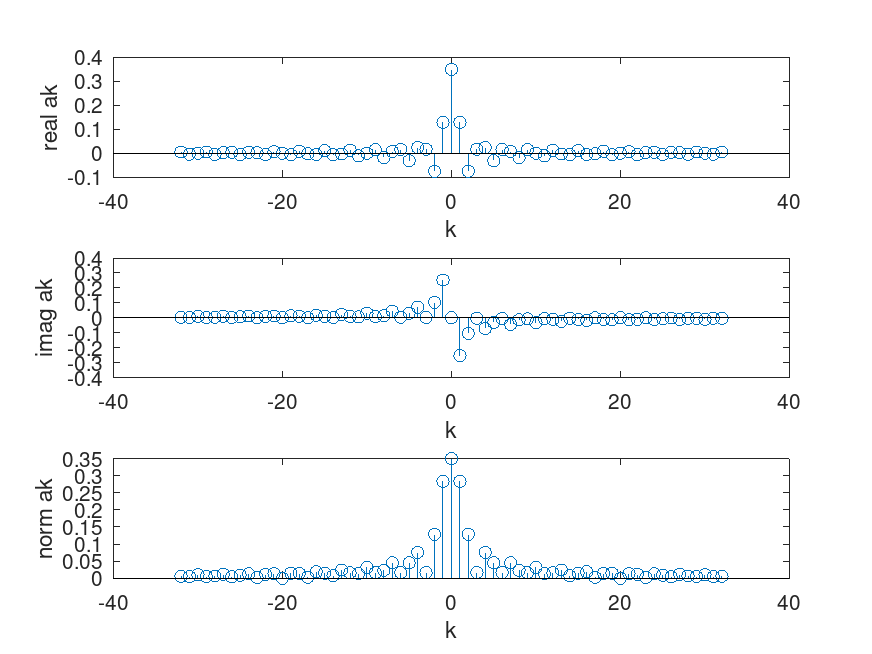
\includegraphics[width=0.7\linewidth]{code/dominio_frecuencia_alpha}
	\caption{Dominio de la frecuencia ejemplo \ref{tren.de.pulsos}}
	\label{fig:dominiofrecuenciaalpha}
\end{figure}

\begin{figure}
	\centering
	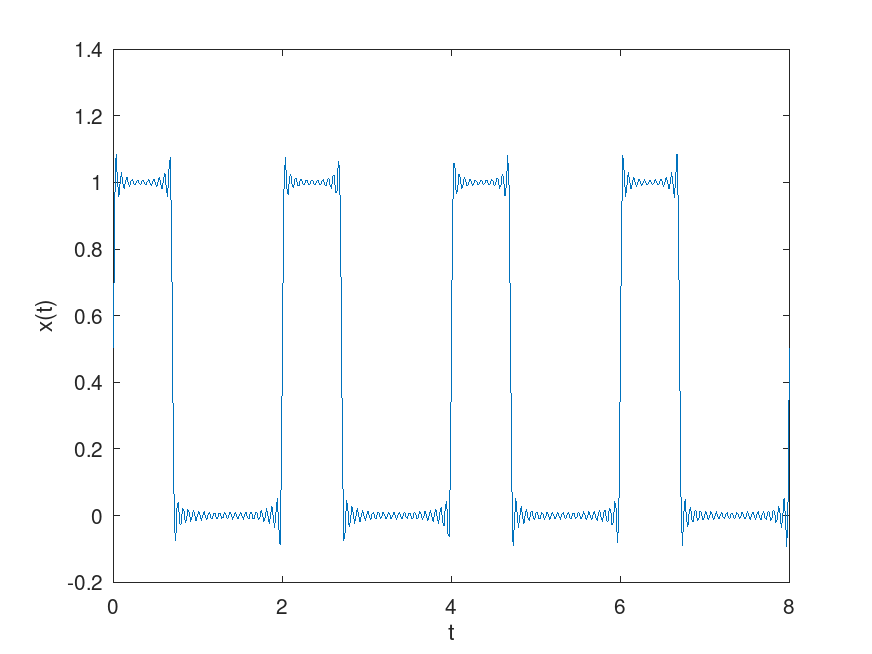
\includegraphics[width=0.7\linewidth]{code/dominio_tiempo_alpha}
	\caption{Dominio del tiempo ejemplo \ref{tren.de.pulsos}}
	\label{fig:dominiotiempoalpha}
\end{figure}

\subsection{Tren de pulsos desfasados \label{tren.de.pulsos.desplazados}}

\begin{enumerate}
\item  Calculemos la serie de Fourier de la se\~{n}al definida por 
\begin{equation}
x_{2}\left( t\right) = x_{2}\left(t + T\right) \left\{ 
\begin{array}{cc}
0, & 0 < t \leq T_{d}, \\
1, & T_{d} < t \leq T_{d} + T_{1}, \\ 
0, & T_{d} + T_{1} < t \leq T.
\end{array}
\right.
\end{equation}
Observemos que
\begin{equation}
x_{2}(t) = x_{1}(t - T_{d}),
\end{equation}
por lo que decimos que $x_{2}(t)$ es un tren de pulsos desfasados (desplazados en el tiempo).

\item Consideremos la ec. (\ref{anafs}), que en este caso se escribe como
\begin{equation}
T \, a_{k}=\int_{T_{d}}^{T_{d} + T_{1}} e^{-j \, k \, \frac{2 \, \pi }{T}t} \, dt.
\end{equation}

\item Para $k = 0$, obtenemos
\begin{equation}
T \, a_{k}=\int_{T_{d}}^{T_{d} + T_{1}} e^{-j \, 0 \, \frac{2 \, \pi }{T}t} \, dt,
\end{equation}
o, resolviendo la integral
\begin{equation}
T \, a_{k}=\int_{T_{d}}^{T_{d} + T_{1}} 1 \, dt = \left[ t \right]_{T_{d}}^{T_{d}+T_{1}} = T_{1}.
\end{equation}

\item Para $k \neq 0$, obtenemos
\begin{equation}
T \, a_{k}=\int_{T_{d}}^{T_{d} + T_{1}} \, e^{-j \, k \, \frac{2 \, \pi }{T}t} \, dt,
\end{equation}
o
\begin{equation}
T \, a_{k}=\frac{1}{-j \, k \, \frac{2 \, \pi }{T}} \int_{T_{d}}^{T_{d} + T_{1}} \, e^{-j \, k \, \frac{2 \, \pi }{T}\,t} \, d(-j \, k \, \frac{2 \, \pi }{T} \, t).
\end{equation}
Finalmente
\begin{equation}
T \, a_{k}=\frac{1}{-j \, k \, \frac{2 \, \pi }{T}}  \left[e^{-j \, k \, \frac{2 \, \pi }{T}\,t} \right]_{T_{d}}^{T_{d} + T_{1}}.
\end{equation}
Observe que podemos extraer un factor com\'{u}n de la integral
\begin{equation}
T \, a_{k}=\frac{e^{-j \, k \frac{2 \, \pi}{T} \, T_{d}}}{-j \, k \, \frac{2 \, \pi }{T}} \left[e^{-j \, k \, \frac{2 \, \pi }{T}\,t} \right]_{0}^{T_{1}},
\end{equation}
y as\'{\i} obtener finalmente
\begin{equation}
T \, a_{k}=\frac{e^{-j \, k \frac{2 \, \pi}{T} \, T_{d}}}{-j \, k \, \frac{2 \, \pi }{T}} \, 
\left(e^{-j \, k \, \frac{2 \, \pi \, T_{1}}{T}} - 1\right).
\end{equation}

\item Por lo tanto, los coeficientes de la serie de Fourier son
\begin{equation}
\left\{
\begin{array}{ll}
k=0 \rightarrow & a_{0} = \frac{T_{1}}{T}, \\ 
\\
k \neq 0 \rightarrow & a_{k}= e^{-j \, k \frac{2 \, \pi}{T} \, T_{d}} \, \frac{T_{1}}{T} \,
\frac{\left(1 - e^{-j \, k \, \frac{2 \, \pi \, T_{1}}{T}}\right)}{j \, k \, \frac{2 \, \pi \, T_{1}}{T}}.
\end{array}
\right.
\end{equation}

\item Comparando los coeficientes de $x_{1}(t)$ con los de $x_{2}(t) = x_{1}(t+T_{d})$ podemos notar
que solamente difieren en un factor $e^{-j \, k \frac{2 \, \pi}{T} \, T_{d}}$, cuya magnitud es $1$ y 
su fase es proporcional a $k$.
\end{enumerate}

\lstinputlisting[language=Octave]{./code/bravo.m}

\begin{figure}
	\centering
	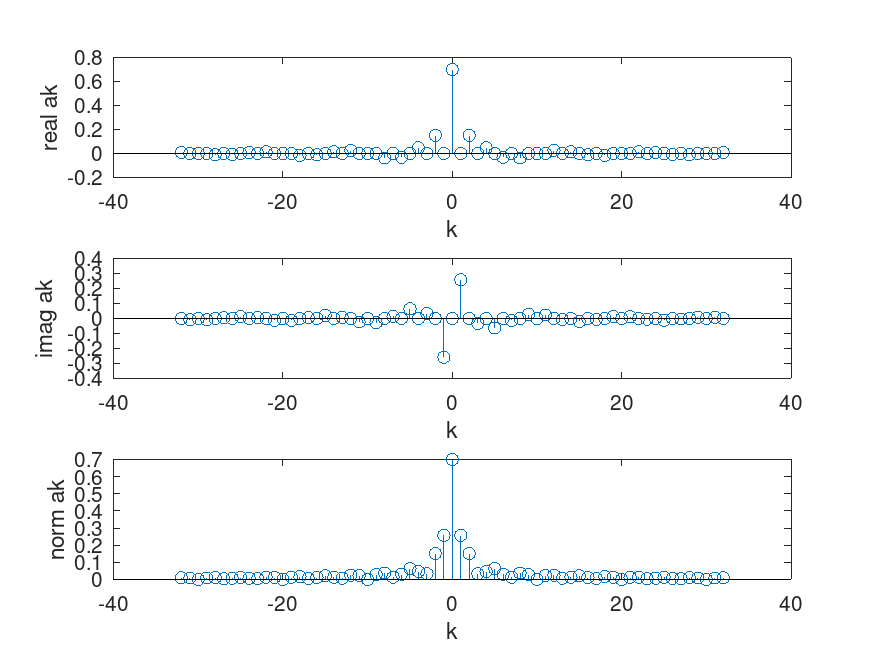
\includegraphics[width=0.7\linewidth]{code/dominio_frecuencia_bravo}
	\caption{Dominio de la frecuencia ejemplo \ref{tren.de.pulsos.desplazados}}
	\label{fig:dominiofrecuenciabravo}
\end{figure}

\begin{figure}
	\centering
	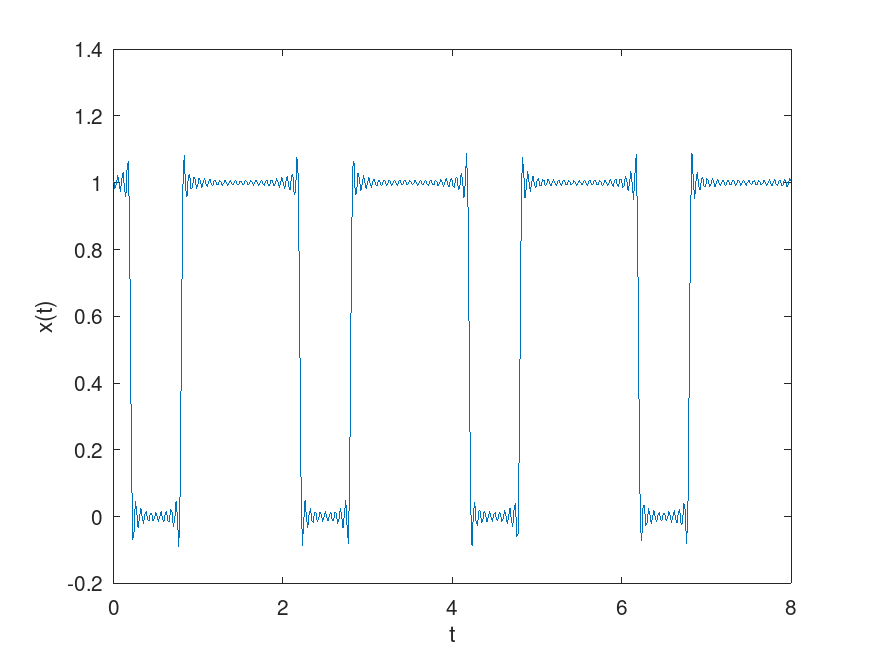
\includegraphics[width=0.7\linewidth]{code/dominio_tiempo_bravo}
	\caption{Dominio del tiempo ejemplo \ref{tren.de.pulsos.desplazados}}
	\label{fig:dominiotiempobravo}
\end{figure}

\subsection{Tren de pulsos alternados \label{tren.de.pulsos.impar}}

\begin{enumerate}
\item  Calculemos la serie de Fourier de la se\~{n}al definida por 
\begin{equation}
x_{3}\left( t\right) = x_{3}\left(t + 2 \, T \right) = 
\left\{ 
\begin{array}{cc}
-1, & -T<t \leq 0, \\ 
1, & 0 < t \leq T
\end{array}
\right.
\end{equation}

\item Entonces podemos escribir para $k = 0$,
\begin{equation}
	2 \, T \, a_{0}=
	-\int_{-T}^{0}e^{-j \, 0 \, \frac{2 \, \pi }{2 \, T} \, t} \, dt + 
	\int_{0}^{T}e^{-j \, 0 \, \frac{2 \, \pi }{2 \, T} \, t} \, dt =
	-\int_{-T}^{0} 1 \, dt + 
\int_{0}^{T} 1 \, dt = 0.
\end{equation}

\item Para $k \neq 0$ tenemos
\begin{equation}
	2 \, T \, a_{0}=
	-\int_{-T}^{0}e^{-j \, k \, \frac{2 \, \pi }{2 \, T} \, t} \, dt + 
	\int_{0}^{T}e^{-j \, k \, \frac{2 \, \pi }{2 \, T} \, t} \, dt,
\end{equation}
donde
\begin{equation}
	\int_{-T}^{0}e^{-j \, k \, \frac{2 \, \pi }{2 \, T} \, t} \, d (-j \, k \, \frac{2 \, \pi }{2 \, T})\,t = \left[e^{-j \, k \, \frac{\pi }{T} \, t}\right]_{-T}^{0} = 1 - e^{j \, k \, \frac{\pi }{T} \, T} = 1 - e^{j \, k \, \pi},
\end{equation}
y
\begin{equation}
	\int_{0}^{T}e^{-j \, k \, \frac{2 \, \pi }{2 \, T} \, t} \, d(-j \, k \, \frac{2 \, \pi }{2 \, T}) \, t = \left[e^{-j \, k \, \frac{2 \, \pi }{2 \, T} \, t}\right]_{0}^{T} = e^{-j \, k \, \frac{\pi }{T} \, T} - 1 = e^{-j \, k \, \pi} - 1.
\end{equation}

\item Por lo tanto resulta
\begin{equation}
 2 \, T \, a_{k}=
 \frac{- 1 + e^{j \, k \, \pi} + e^{-j \, k \, \pi} - 1}{-j \, k \, \frac{\pi}{T}}.
\end{equation}
\item Simplificando
\begin{equation}
	a_{k}=
	\frac{\frac{e^{j \, k \, \pi} + e^{-j \, k \, \pi}}{2} - 1}{-j \, k \, \pi}.
\end{equation}
podemos escribir
\begin{equation}
 a_{k}= j \, 
 \frac{cos(k \, \pi) - 1}{k \, \pi}.
\end{equation}
\item Observemos que cuando $k = 2 \, p$, $cos(k \, \pi) = cos(p \, 2 \, \pi) = 1$ y por lo tanto 
\begin{equation}a_{2 \, p} = 0.\end{equation}
Cuando $k = 2 \, p + 1$, entonces $cos((2 \, p + 1) \, \pi) = -1$ y 
\begin{equation}a_{2 \, p + 1} = \frac{-2 \, j}{k \, \pi}.\end{equation}

\end{enumerate}

\lstinputlisting[language=Octave]{./code/charlie.m}

\begin{figure}
	\centering
	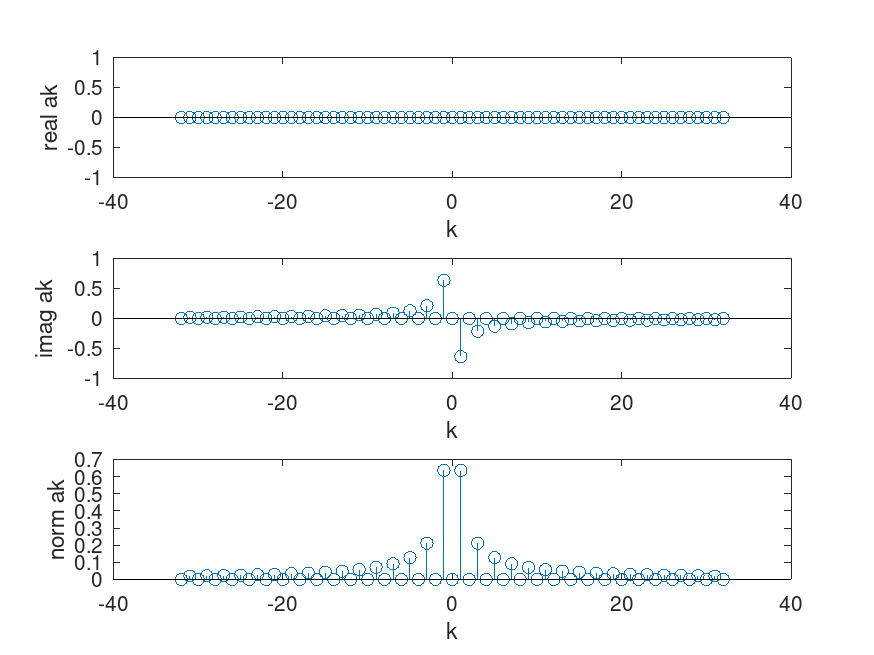
\includegraphics[width=0.7\linewidth]{code/dominio_frecuencia_charlie}
	\caption{Dominio de la frecuencia ejemplo \ref{tren.de.pulsos.impar}}
	\label{fig:dominiofrecuenciacharlie}
\end{figure}

\begin{figure}
	\centering
	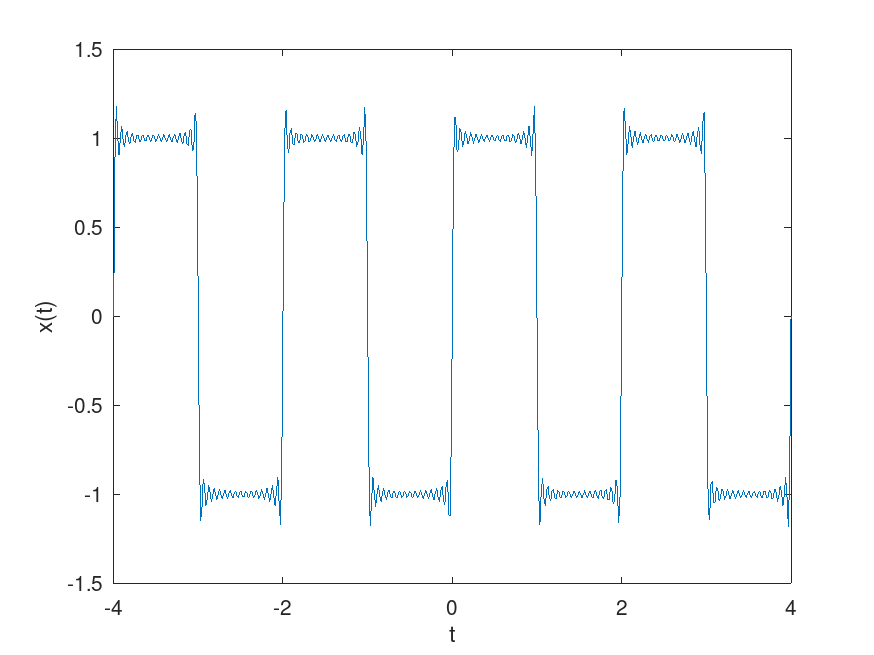
\includegraphics[width=0.7\linewidth]{code/dominio_tiempo_charlie}
	\caption{Dominio del tiempo ejemplo \ref{tren.de.pulsos.impar}}
	\label{fig:dominiotiempocharlie}
\end{figure}

\subsection{Suma de se\~{n}ales peri\'{o}dicas \label{tren.de.pulsos.suma}}

\begin{enumerate}
\item  Calculemos la serie de Fourier de la se\~{n}al definida por 
\begin{equation}
x_{4}\left( t\right) = x_{4}(t+4) \left\{
\begin{array}{cc}
1, & 0 < t \leq 1, \\
0, & 1 < t \leq 2, \\ 
-1, & 2 < t \leq 3, \\
0, & 3 < t \leq 4.
\end{array}
\right. \label{squarewave}
\end{equation}
En este caso, $x_{4}(t) = x_{1}(t) - x_{1}(t-T_{d})$, con $T = 4$, $T_{1} = 1$ y $T_{d} = 2$. Si escribimos
\begin{equation}
	x_{4}(t) = \sum_{k=-\infty}^{\infty} b_{k} \, e^{j \, k \, \frac{2 \, \pi \, t}{T}},
\end{equation}
debería ser
\begin{equation}
	b_{k} = a_{k} - a_{k} \, e^{-j \, k \, \frac{2 \, \pi \, T_{d}}{T}} = a_{k} \, (1 - e^{-j \, k \, \frac{2 \, \pi \, T_{d}}{T}}).
\end{equation}

\item Para comprobarlo, escribimos
\begin{equation}
	x_{1}(t) = \frac{1}{4} + \sum_{k=1}^{\infty} 
     \frac{1}{4} \, \frac{\left(1 - e^{-j \, k \, \frac{2 \, \pi}{4}}\right)}{j \, k \, \frac{2 \, \pi}{4}} \, e^{j \, k \, \frac{2 \, \pi \, t}{4}}
     +
     \frac{1}{4} \, \frac{\left(1 - e^{j \, k \, \frac{2 \, \pi}{4}}\right)}{-j \, k \, \frac{2 \, \pi}{4}} \, e^{-j \, k \, \frac{2 \, \pi \, t}{4}},
\end{equation}
\item También podemos escribir
\begin{equation}
	x_{1}(t-2) = \frac{1}{4} \left(1 + \sum_{k=1}^{\infty} 
	\frac{\left(1 - e^{-j \, k \, \frac{2 \, \pi}{4}}\right)}{j \, k \, \frac{2 \, \pi}{4}} \, e^{j \, k \, \frac{2 \, \pi \, (t-2)}{4}}
	+
	\frac{\left(1 - e^{j \, k \, \frac{2 \, \pi}{4}}\right)}{-j \, k \, \frac{2 \, \pi}{4}} \, e^{-j \, k \, \frac{2 \, \pi \, (t-2)}{4}}\right).
\end{equation}
y por lo tanto
\begin{equation}
	x_{1}(t-2) = \frac{1}{4} \left(1 + \sum_{k=1}^{\infty} 
	\frac{\left(1 - e^{-j \, k \, \frac{\pi}{2}}\right)}{j \, k \, \frac{\pi}{2}} \, e^{-j \, k \, \pi} \,
	e^{j \, k \, \frac{\pi \, t}{2}}
	+
	\frac{\left(1 - e^{j \, k \, \frac{\pi}{2}}\right)}{-j \, k \, \frac{\pi}{2}} \, e^{j \, k \, \pi}
	e^{-j \, k \, \frac{\pi \, t}{2}} \right).
\end{equation}

\item Por lo tanto, podemos ver que
\begin{equation}
	a_{0} = \frac{1}{4} - \frac{1}{4} = 0,
\end{equation}
y
\begin{equation}
	a_{k} = \frac{1}{4}	\, \frac{\left(1 - e^{-j \, k \, \frac{\pi}{2}}\right)}{j \, k \, \frac{\pi}{2}} \, (1 - e^{-j \, k \, \pi}) =
	\frac{1}{4}	\,
	\frac{\left(1 - e^{-j \, k \, \frac{ \pi}{2}}\right)}{j \, k \, \frac{\pi}{2}} \, (1 - e^{-j \, k \, \pi}).
\end{equation}

\end{enumerate}

\lstinputlisting[language=Octave]{./code/delta.m}

\begin{figure}
	\centering
	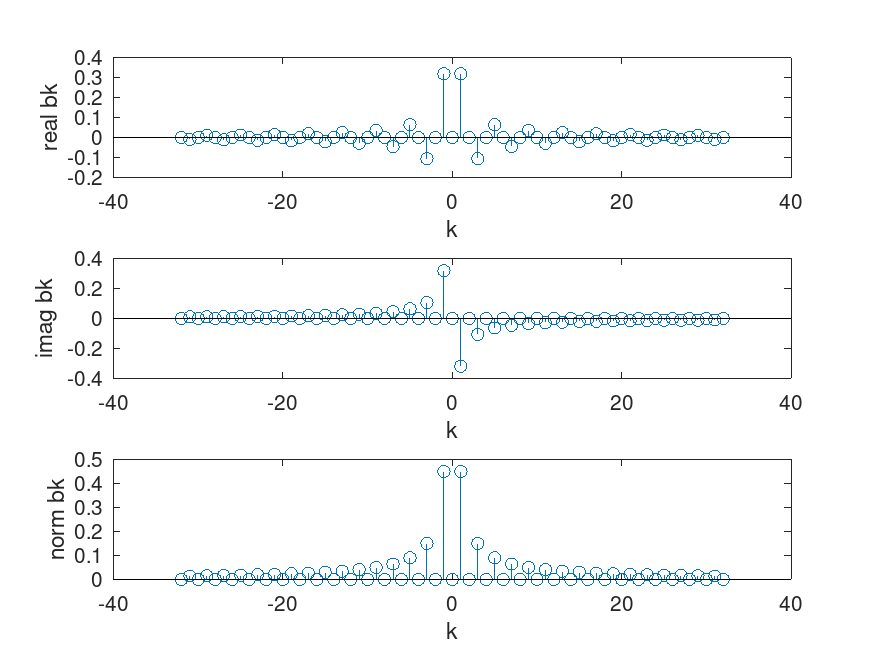
\includegraphics[width=0.7\linewidth]{code/dominio_frecuencia_delta}
	\caption{Dominio de la frecuencia ejemplo \ref{tren.de.pulsos.suma}}
	\label{fig:dominiofrecuenciadelta}
\end{figure}

\begin{figure}
	\centering
	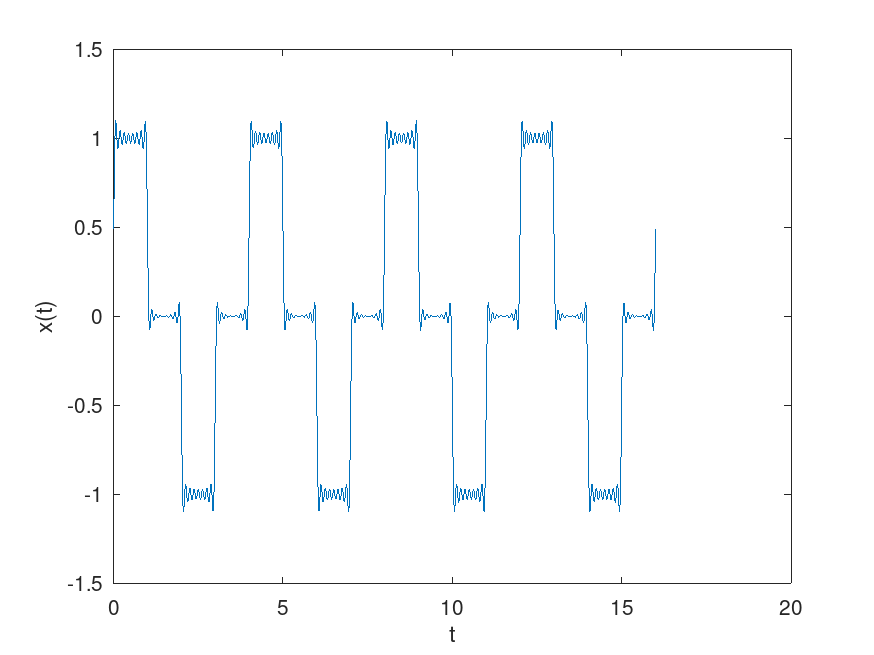
\includegraphics[width=0.7\linewidth]{code/dominio_tiempo_delta}
	\caption{Dominio del tiempo ejemplo \ref{tren.de.pulsos.suma}}
	\label{fig:dominiotiempodelta}
\end{figure}

\subsection{Una función periódica par \label{funcion.par}}

\begin{enumerate}
\item  Calculemos la serie de Fourier de la se\~{n}al definida por
\begin{equation}
x_{4}\left( t\right) = x_{4}(t+2 \, T)\left\{ 
\begin{array}{cc}
0   & -T < t \leq -T_{1}, \\
1  & -T_{1} < t \leq T_{1}, \\ 
0  & T_{1} < t \leq T.
\end{array}
\right. \label{squarewaveone.1}
\end{equation}
\item La ecuación de análisis (\ref{anafs}) para este caso es
\begin{equation}
2 \, T \, a_{k} = 
\int_{-T_{1}}^{T_{1}} e^{-j \, k \,\frac{2 \, \pi }{2 \, T} \, t} \, dt.
\end{equation}
\item Para $k = 0$,
\begin{equation}
2 \, T \, a_{0} = 
\int_{-T_{1}}^{T_{1}} e^{-j \, 0 \,\frac{2 \, \pi }{2 \, T} \, t} \, dt = 2 \, T_{1}.
\end{equation}
\begin{equation}
a_{0} = \frac{2 \, T_{1}}{2 \, T} = \frac{T_{1}}{T}.
\end{equation}
\item Para $k \neq 0$,
\begin{equation}
2 \, T \, a_{k} = 
\frac{\int_{-T_{1}}^{T_{1}} e^{-j \, k \,\frac{\pi }{T} \, t} \, d(-j \, k \,\frac{\pi }{T})t}{-j \, k \,\frac{\pi }{T}}.
\end{equation}
\item Evaluamos la integral
\begin{equation}
2 \, T \, a_{k} = 
\frac{\left[e^{\frac{-j \, k \, \pi \, t}{T}}\right]_{-T_{1}}^{T_{1}}}{\frac{j \, k \, \pi }{T}} =
\frac{e^{\frac{-j \, k \, \pi \, T_{1}}{T}}-
	  e^{\frac{j \, k \, \pi \, T_{1}}{T}}}{\frac{-j \, k \, \pi }{T}}.
\end{equation}
\item Simplificamos expresiones
\begin{equation}
a_{k} = \frac{e^{\frac{-j \, k \, \pi \, T_{1}}{T}}-
	e^{\frac{j \, k \, \pi \, T_{1}}{T}}}{-2 \, j \, k \, \pi} = 
    \frac{e^{\frac{j \, k \, \pi \, T_{1}}{T}}-
	e^{\frac{-j \, k \, \pi \, T_{1}}{T}}}{2 \, j \, k \, \pi} = 
    \frac{sin(\frac{k \, \pi \, T_{1}}{T})}{k \, \pi}
.
\end{equation}
\item Multiplicando y dividiendo
\begin{equation}
	a_{k} =  \frac{T_{1}}{T} \, \frac{sin(\frac{k \, \pi \, T_{1}}{T})}{k \, \pi \, \frac{T_{1}}{T}}
	.
\end{equation}
\item
Resumiendo
\begin{equation}
 a_{0} = \frac{T_{1}}{T_{2}},
\end{equation}
y
\begin{equation}
	a_{k} =  \frac{T_{1}}{T} \, \frac{sin(\frac{k \, \pi \, T_{1}}{T})}{k \, \pi \, \frac{T_{1}}{T}}
.
\end{equation}

\end{enumerate}

\lstinputlisting[language=Octave]{./code/echo.m}

\begin{figure}
	\centering
	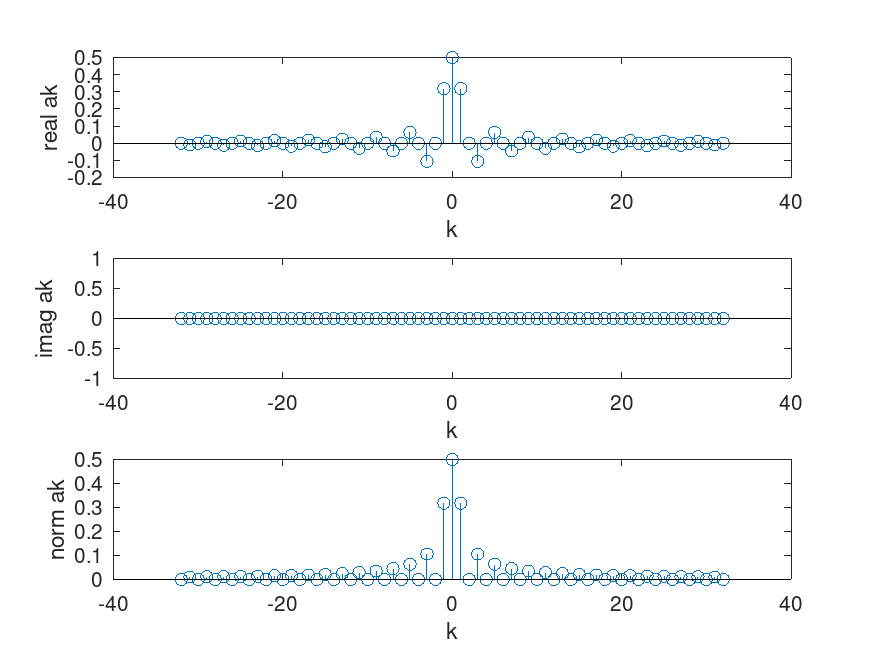
\includegraphics[width=0.7\linewidth]{code/dominio_frecuencia_echo}
	\caption{Dominio de la frecuencia ejemplo \ref{funcion.par}}
	\label{fig:dominiofrecuenciaecho}
\end{figure}

\begin{figure}
	\centering
	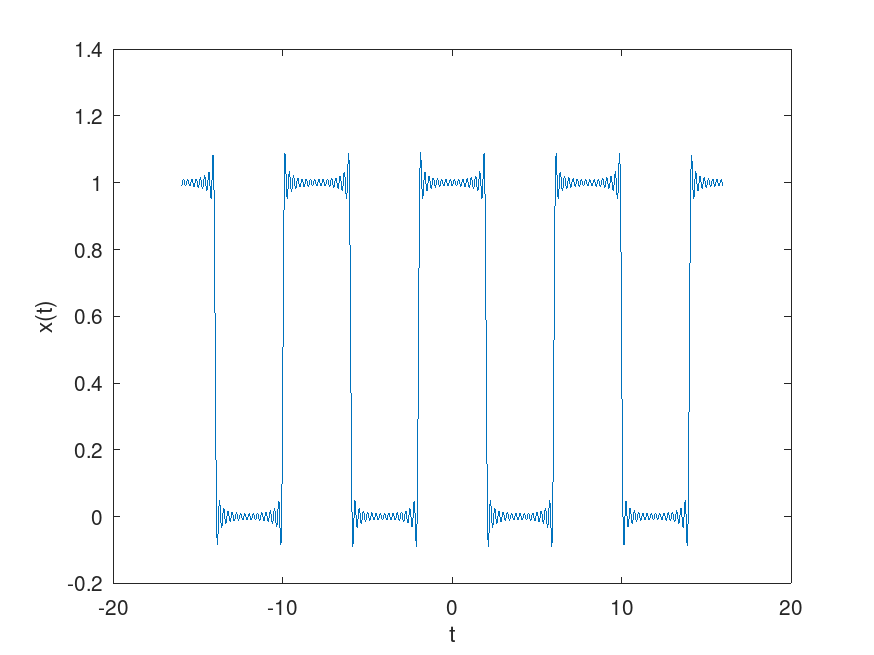
\includegraphics[width=0.7\linewidth]{code/dominio_tiempo_echo}
	\caption{Dominio del tiempo ejemplo \ref{funcion.par}}
	\label{fig:dominiotiempoecho}
\end{figure}

\subsection{Una función periódica impar \label{funcion.impar}}

\begin{enumerate}
	\item  Calculemos la serie de Fourier de la se\~{n}al definida por
	\begin{equation}
		x_{5}\left( t\right) = x_{4}(t+2 \, T)\left\{ 
		\begin{array}{cc}
			0   & -T < t \leq -T_{1}, \\
			-1  & -T_{1} < t \leq 0, \\ 
			1   & 0 < t \leq T_{1}, \\
			0  & T_{1} < t \leq T.
		\end{array}
		\right. \label{squarewavetwo.1}
	\end{equation}
	\item La ecuación de análisis (\ref{anafs}) para $k = 0$ es
    \begin{equation}
	2 \, T \, a_{0} = 
	-\left(\int_{-T_{1}}^{0}  \, dt\right)
	+\left(\int_{0}^{T_{1}}  \, dt\right)	= 0.
    \end{equation}

	\item La ecuación de análisis (\ref{anafs}) para $k \neq 0$ es
	\begin{equation}
		2 \, T \, a_{k} = 
		-\left(\int_{-T_{1}}^{0} e^{-j \, k \,\frac{2 \, \pi }{2 \, T} \, t} \, dt\right)
		+\left(\int_{0}^{T_{1}} e^{-j \, k \,\frac{2 \, \pi }{2 \, T} \, t} \, dt\right).
		\label{squarewavetwo.2}
	\end{equation}

	\item Para resolver (\ref{squarewavetwo.2}) multiplicamos y dividimos por $-j \, k \, \frac{\pi}{T}$
\begin{equation}
	2 \, T \, a_{k} = 
	-\frac{\left[e^{-j \, k \,\frac{\pi }{T} \, t} \right]_{-T_{1}}^{0}}{-j \, k \, \frac{\pi}{T}} 
	+\frac{\left[e^{-j \, k \,\frac{\pi }{T} \, t} \right]_{0}^{T_{1}}}{-j \, k \, \frac{\pi}{T}}.
	\label{squarewavetwo.3}
\end{equation}

	\item Escribamos
\begin{equation}
	-j \, 2 \, T \, k \, \frac{\pi}{T} \, a_{k} = 
	-\left[e^{-j \, k \,\frac{\pi }{T} \, t} \right]_{-T_{1}}^{0} 
	+\left[e^{-j \, k \,\frac{\pi }{T} \, t} \right]_{0}^{T_{1}}.
	\label{squarewavetwo.4}
\end{equation}

\item 
\begin{equation}
	-j \, 2 \, k \, \pi \, a_{k} = 
-\left(1 - e^{j \, k \,\frac{\pi }{T} \, T_{1}} \right) 
+\left(e^{-j \, k \,\frac{\pi }{T} \, T_{1}} - 1 \right).
	\label{squarewavetwo.5}
\end{equation}
\item 
\begin{equation}
	-j \, 2 \, k \, \pi \, a_{k} = 
	e^{j \, k \,\frac{\pi }{T} \, T_{1}}
	+e^{-j \, k \,\frac{\pi }{T} \, T_{1}} - 2.
	\label{squarewavetwo.6}
\end{equation}
\item 
\begin{equation}
	-j \, 2 \, k \, \pi \, a_{k} = 
	e^{j \, k \,\frac{\pi }{T} \, T_{1}}
	+e^{-j \, k \,\frac{\pi }{T} \, T_{1}} - 2.
	\label{squarewavetwo.7}
\end{equation}
\item 
\begin{equation}
	a_{k} = 
	\frac{2 - e^{j \, k \,\frac{\pi }{T} \, T_{1}}
	-e^{-j \, k \,\frac{\pi }{T} \, T_{1}}}{j \, 2 \, k \, \pi \,}.
	\label{squarewavetwo.8}
\end{equation}
\item 
\begin{equation}
	a_{k} = \frac{T_{1}}{T} \,
	\frac{1 - cos(k \,\frac{\pi }{T} \, T_{1})}{
	j \, k \, \pi \, \frac{T_{1}}{T}}.
	\label{squarewavetwo.9}
\end{equation}
\end{enumerate}

\lstinputlisting[language=Octave]{./code/foxtrot.m}

\begin{figure}
	\centering
	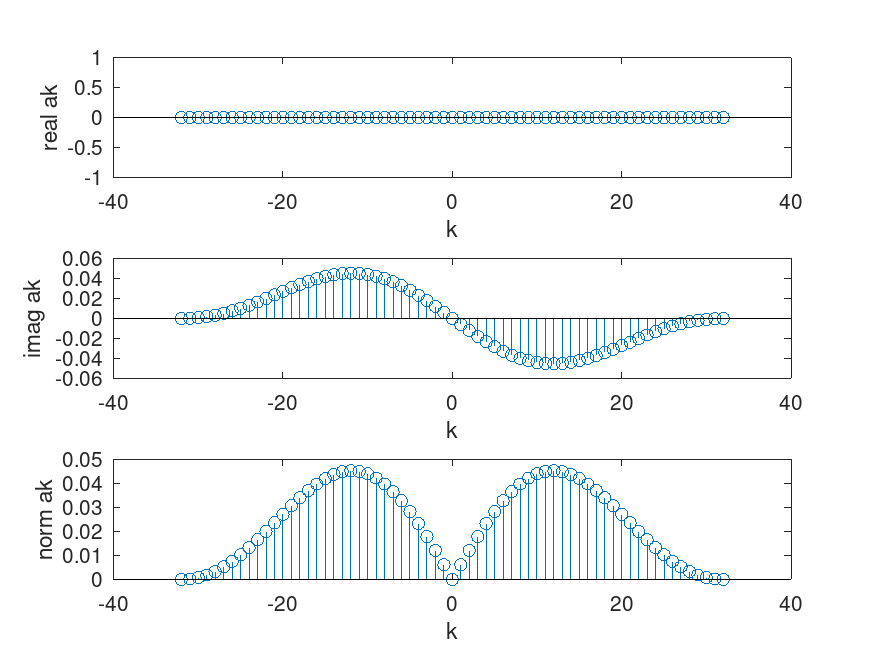
\includegraphics[width=0.7\linewidth]{code/dominio_frecuencia_foxtrot}
	\caption{Dominio de la frecuencia ejemplo \ref{funcion.impar}}
	\label{fig:dominiofrecuenciafoxtrot}
\end{figure}

\begin{figure}
	\centering
	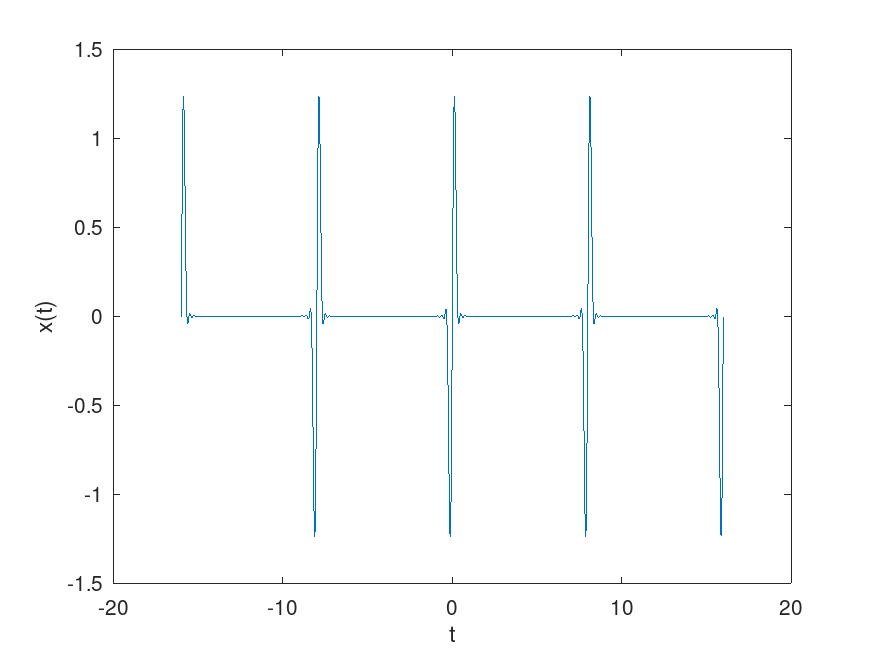
\includegraphics[width=0.7\linewidth]{code/dominio_tiempo_foxtrot}
	\caption{Dominio del tiempo ejemplo \ref{funcion.impar}}
	\label{fig:dominiotiempofoxtrot}
\end{figure}

\section{Sistema lineal excitado con una serie de Fourier}

\begin{enumerate}
\item Supongamos que tenemos un sistema lineal invariante en el tiempo con una respuesta al impulso $h(t)$. Vamos a calcular la salida $y(t)$ para una entrada
\begin{equation}
	x(t) = \sum_{k=-\infty}^{\infty} a_{k} \, e^{j \, k \, \frac{2 \, \pi}{T} \, t}. 
	\label{conv.tc.seriedefourier.alpha}
\end{equation}

\item Para evaluar la integral de convolución, emplearemos la fórmula
\begin{equation}
	y(t) = \int_{-\infty}^{\infty} h(v) \, x(t - v) \, dv. 
	\label{conv.tc.seriedefourier.bravo}	
\end{equation}

\item Reemplazando (\ref{conv.tc.seriedefourier.alpha}) en (\ref{conv.tc.seriedefourier.bravo}) obtenemos
\begin{equation}
	y(t) = \int_{-\infty}^{\infty} h(v) \, \left(
	\sum_{k=-\infty}^{\infty} a_{k} \, e^{j \, k \, \frac{2 \, \pi}{T} \, (t-v)}
	\right)
	dv. 
	\label{conv.tc.seriedefourier.charlie}	
\end{equation}
\item Intercambiamos la posición del signo de integral con el signo de sumatoria
y factoreamos la exponencial
\begin{equation}
	y(t) = \sum_{k=-\infty}^{\infty} 
	\int_{-\infty}^{\infty} h(v) \, 
	 a_{k} \, e^{j \, k \, \frac{2 \, \pi}{T} \, t} \, e^{-j \, k \, \frac{2 \, \pi}{T} \, v}
	dv. 
	\label{conv.tc.seriedefourier.delta}	
\end{equation}
\item Podemos extraer el factor $a_{k} \, e^{j \, k \, \frac{2 \, \pi}{T} \, t}$ fuera de las integrales en (\ref{conv.tc.seriedefourier.delta})
\begin{equation}
	y(t) = \sum_{k=-\infty}^{\infty} 
	\left(\int_{-\infty}^{\infty} h(v) \, 
	 \, e^{-j \, k \, \frac{2 \, \pi}{T} \, v}
	dv\right) \, a_{k} \, e^{j \, k \, \frac{2 \, \pi}{T} \, t}.
	\label{conv.tc.seriedefourier.echo}	
\end{equation}
\item En la ecuación (\ref{conv.tc.seriedefourier.echo}) podemos definir
\begin{equation}
	H(k \, \frac{2 \, \pi}{T}) = \int_{-\infty}^{\infty} h(v) \, 
	\, e^{-j \, k \, \frac{2 \, \pi}{T} \, v}
	dv,
\end{equation}
y escribir
\begin{equation}
	y(t) = \sum_{k=-\infty}^{\infty} 
	 H(j \, k \, \frac{2 \, \pi}{T}) \, a_{k} \, e^{j \, k \, \frac{2 \, \pi}{T} \, t}.
	\label{conv.tc.seriedefourier.foxtrot}	
\end{equation}

\item Los factores $H(j \, k \, \frac{2 \, \pi}{T})$ son evaluaciones de la transformada de Fourier $H(j \, \omega)$ para los valores de frecuencia $j \, k \, \frac{2 \, \pi}{T}$. Si elegimos los valores de $H(j \, k \, \frac{2 \, \pi}{T})$ en forma adecuada, podemos procesar la señal de entrada para obtener una salida conveniente o adecuada. Esto es el principio matemático de los filtros de señal.

\end{enumerate}
%\section{Modulación}
%
%¿Qué pasa cuando multiplicamos dos funciones periódicas?
%
%\subsection{El caso más sencillo}
%
%Consideremos la multiplicación de dos señales períodicas con períodos que no son necesariamente iguales
%\begin{equation}
% x_{1}(t) = e^{j \, \frac{2 \, \pi}{T_{1}} \, t},
%\end{equation}
%\begin{equation}
% x_{2}(t) = e^{j \, \frac{2 \, \pi}{T_{2}} \, t},
%\end{equation}
%y
%\begin{equation}
% y(t) = x_{1}(t) \, x_{2}(t) = e^{j \, \frac{2 \, \pi}{T_{1}} \, t} \, e^{j \, \frac{2 \, \pi}{T_{2}} \, t}.
%\end{equation}
%La pregunta es ¿Cuál es el período $T$ de $y(t)$?
%Si hacemos
%\begin{equation}
% y(t) = e^{j \, \frac{2 \, \pi}{T_{1}} \, t} \, e^{j \, \frac{2 \, \pi}{T_{2}} \, t} = 
% e^{j \, \left(\frac{1}{T_{1}} + \frac{1}{T_{2}}\right) \, 2 \, \pi \, t},
%\end{equation}
%que debe ser
%\begin{equation}
% y(t) = e^{j \, \frac{2 \, \pi}{T} \, t} =
% e^{j \, \left(\frac{1}{T_{1}} + \frac{1}{T_{2}}\right) \, 2 \, \pi \, t}.
%\end{equation}
%Por lo tanto resulta
%\begin{equation}
% \frac{1}{T} = \frac{1}{T_{1}} + \frac{1}{T_{2}}.
%\end{equation}
%
%\subsection{Una serie de Fourier con $M$ armónicas multiplicada por una exponencial imaginaria}
%
%Consideremos ahora el caso de una serie de Fourier
%\begin{equation}
% x_{1}(t) = \sum_{k=-M}^{M} a_{k} \, e^{j \, k \, \frac{2 \, \pi}{T_{1}} \, t},
%\end{equation}
%y el producto
%\begin{equation}
% y(t) =  \left(
% \sum_{k=-M}^{M} a_{k} \, e^{j \, k \, \frac{2 \, \pi}{T_{1}} \, t}
% \right) \, e^{j \, \frac{2 \, \pi}{T_{2}} \, t}.
%\end{equation}
%Por la propiedad distributiva del producto respecto a la suma
%\begin{equation}
% y(t) =  
% \sum_{k=-M}^{M} a_{k} \, e^{j \, (k \, \frac{2 \, \pi}{T_{1}} +  \frac{2 \, \pi}{T_{2}})\, t}
%,
%\end{equation}
%podemos escribir
%\begin{equation}
% y(t) =  
% \sum_{k=-M}^{M} a_{k} \, e^{j \, (\frac{k}{T_{1}} +  \frac{1}{T_{2}})\, 2 \, \pi \, t}
%.
%\end{equation}
%Observe que en esta ecuación, no tenemos una serie de Fourier propiamente dicha porque en
%\begin{equation}
%	\frac{k}{T_{1}} +  \frac{1}{T_{2}} \neq \frac{p}{Q \, T},
%\end{equation}
%no tenemos una expresión de donde obtener $T$ para $Q \in N$, $p \in N$.
%
%\subsection{Una serie de Fourier con $M$ armónicas multiplicada por una función cos}
%
%Considerando
%\begin{equation}
%	p(t) =  \left(
%	\sum_{k=-M}^{M} a_{k} \, e^{j \, k \, \frac{2 \, \pi}{T_{1}} \, t}
%	\right) \, e^{j \, \frac{2 \, \pi}{T_{2}} \, t}, 
%\end{equation}
%y
%\begin{equation}
%	q(t) =  \left(
%	\sum_{k=-M}^{M} a_{k} \, e^{j \, k \, \frac{2 \, \pi}{T_{1}} \, t}
%	\right) \, e^{-j \, \frac{2 \, \pi}{T_{2}} \, t}, 
%\end{equation}
%podemos escribir
%\begin{equation}
%	r(t) = p(t) + q(t) =
%	\left( 
%	\sum_{k=-M}^{M} a_{k} \, e^{j \, k \, \frac{2 \, \pi}{T_{1}} \, t} \, e^{j \, \frac{2 \, \pi}{T_{2}} \, t} 	
%	\right) +
%	\left( 
%    \sum_{k=-M}^{M} a_{k} \, e^{j \, k \, \frac{2 \, \pi}{T_{1}} \, t} \, e^{-j \, \frac{2 \, \pi}{T_{2}} \, t} 	
%    \right).
%\end{equation}
%\begin{equation}
%	r(t) = p(t) + q(t) =
%	\sum_{k=-M}^{M} a_{k} \, 	\left( e^{j \, \left(\frac{k}{T_{1}} + \frac{1}{T_{2}}\right) \, 2 \, \pi \, t} + e^{j \, \left(\frac{k}{T_{1}} - \frac{1}{T_{2}}\right) \, 2 \, \pi \, t}
%	\right).
%\end{equation}

\section{Ejercicios}

% Signals and Systems with Matlab 2009, pages 65 - 67

\begin{enumerate}
\item Obtenga coeficientes de Fourier (para una serie expresada como suma ponderada de exponenciales imaginarias) 
para una se\~{n}al triangular obtenida integrando la se\~{n}al $x_{5}(t)$ definida arriba en la ecuaci\'{o}n (\ref{squarewave}). 
Grafique el espectro correspondiente.

\item Obtenga coeficientes de Fourier (para una serie expresada como suma ponderada de exponenciales imaginarias) 
para una se\~{n}al triangular obtenida integrando la se\~{n}al $x_{6}(t)$ definida arriba en la ecuaci\'{o}n (\ref{squarewaveone.1}). 
Grafique el espectro correspondiente.

\item Obtenga coeficientes de Fourier (para una serie expresada como suma ponderada de exponenciales imaginarias) 
para la se\~{n}al per\'{o}dica $T$, tal que $0 < T_{1} \leq T$, definida como
\begin{equation}
x_{7}(t) = \left\{\begin{array}{cc}
  1 & |t - k \, T| \leq \frac{T_{1}}{2}, \\
    & \\
  0 & |t - k \, T| > \frac{T_{1}}{2},
\end{array} \right.
\end{equation}
Compruebe que los coeficientes se pueden definir como
\begin{equation}
c_{k} = T_{1} \, \frac{sin(k \, \frac{2 \, \pi}{T} \frac{T_{1}}{2})}{k \, \frac{2 \, \pi}{T} \frac{T_{1}}{2}}.
\end{equation}
Explique que sucede cuando $k = 0$.
\item Desplaze la se\~{n}al $x_{5}$ en el tiempo hasta que coincida con la se\~{n}al $x_{7}$. \textquestiondown Que factor es el necesario para modificar los coeficientes de $x_{5}$ para que coincidan con los de $x_{7}$?
\end{enumerate}

 % Series de Fourier de tiempo continuo

\chapter{Transformada de Fourier de tiempo continuo}

\section{Introducci\'{o}n}

\begin{enumerate}

\item   Vamos a ver como podemos \textbf{modificar} el concepto de \textbf{serie de Fourier} \textbf{para estudiar funciones no peri\'{o}dicas} de tiempo continuo.  
Esto nos permite \textbf{definir} el concepto de \textbf{contenido de frecuencias de una se\~{n}al}, a\'{u}n cuando sea no peri\'{o}dica.

\item   Pensemos en el ejemplo (\ref{funcion.par}), donde
\begin{equation}
	a_{0} = \frac{T_{1}}{T_{2}},
\end{equation}
y
\begin{equation}
	a_{k} =  \frac{T_{1}}{T} \, \frac{sin(\frac{k \, \pi \, T_{1}}{T})}{\frac{k \, \pi \, T_{1}}{T}}
	. \label{tf.1}
\end{equation}
\item  Podemos escribir (\ref{tf.1}) de la siguiente forma
        \begin{equation}
           T a_{k}=
	T \, a_{k} =  \left. T_{1} \, \frac{sin(\omega)}{\omega} \right|_{\omega = \frac{k \, \pi \, T_{1}}{T}}
        \end{equation}
        y entonces es evidente que la podemos interpretar como una \textbf{secuencia} formada por \textbf{muestras} de una \textbf{funci\'{o}n envolvente} $T_{1} \, \frac{\sin(\omega)}{\omega}$) donde la variable $\omega $ es continua, y 
        la secuencia $T a_{k}$ está formada por valores igualmente espaciados en 
        frecuencia, con intervalo $\frac{\pi \, T_{1}}{T}$.
        
        \item   Observe que la separaci\'{o}n de las muestras de la envolvente de $T a_{k}$ est\'{a} dada 
        por 
        \begin{equation}
                \omega_{T} = \frac{\pi \, T_{1}}{T}.
        \end{equation}
        Entonces, cuando mayor sea $T$ menor ser\'{a} $\omega_{T}$ y la cantidad de muestras en un intervalo dado de frecuencia ser\'{a} mayor.

        \item  Si fijamos el valor $T_{1}$ (recordando que debe ser $T_{1}<T,$ por hip\'{o}tesis) la envolvente de $T a_{k}$ es independiente de $T$.
\end{enumerate}

\section{Síntesis y análisis}

\subsection{Teor\'{\i}a}

\begin{enumerate}

        \item  Vamos a construir una se\~{n}al $x\left( t\right) $ no peri\'{o}dica como el l\'{\i}mite de 
        una se\~{n}al $\hat{x}\left( t\right) $ peri\'{o}dica cuando el per\'{\i}odo $T$ tiende a 
        $\infty .$ Veamos que pasa con los coeficientes de la serie de Fourier. 
        Recordemos que una se\~{n}al peri\'{o}dica $\hat{x}\left( t\right) =\hat{x}\left( t+T\right) $ 
        se puede escribir como una serie de Fourier mediante la ecuaci\'{o}n de s\'{\i}ntesis 
        \begin{equation}
                \hat{x}\left( t\right) =\sum_{k=-\infty }^{\infty }a_{k} \, e^{j \, k \, \omega_{0} \, t},
        \end{equation}
        donde los coeficientes $a_{k}$ se calculan mediante la ecuaci\'{o}n de an\'{a}lisis 
        \begin{equation}
            a_{k}=\frac{1}{T}\int_{-\frac{T}{2}}^{\frac{T}{2}}\hat{x}\left( t\right) e^{-j \, k \, \omega_{0} \, t}dt.
        \end{equation}

        \item  Definamos la se\~{n}al no peri\'{o}dica $x(t)$ especificando 
        \begin{equation}
                x\left( t\right) =
                        \left\{ \begin{array}{ll}
                                \hat{x}\left( t\right) & \left| t\right| \leq \frac{T}{2}, \\
                                & \\
                                0 & \left| t\right| >\frac{T}{2},
                                \end{array} 
                        \right. \qquad
                        \hat{x}\left( t\right) =\hat{x}\left( t+T\right) .
        \end{equation}
        Entonces los coeficientes de la serie de Fourier son 
        \begin{equation}
           a_{k}=
                  \frac{1}{T}\int_{-\frac{T}{2}}^{\frac{T}{2}}\hat{x}\left( t\right)e^{-j \, k \, \omega_{0} \, t}dt=
                  \frac{1}{T}\int_{-\infty }^{\infty }x\left( t\right)e^{-j \, k \, \omega_{0} \, t}dt.
        \end{equation}
        \textbf{Las dos integrales son iguales en valor porque un per\'{\i}odo de }
        $\hat{x}\left( t\right) $  \textbf{\ coincide con }$x\left( t\right) ,$ 
        \textbf{\ justamente donde se eval\'{u}a la primer integral, y } $x\left(t\right) $
        \textbf{\ es nula para }$\left| t\right| >\frac{T}{2}.$

        \item  Definamos la ecuaci\'{o}n de an\'{a}lisis de la transformada de Fourier como 
        \begin{equation}
                X\left( j \, \omega \right) =\int_{-\infty }^{\infty }x\left( t\right)e^{-j \, \omega \, t} \, dt.
        \end{equation}
        Tenemos que los coeficientes de la serie de Fourier forman la secuencia de valores 
        \begin{equation}
                Ta_{k}=X\left( j \, k \, \omega_{0}\right) .
        \end{equation}

        \item  Usando la ecuaci\'{o}n de s\'{\i}ntesis de la serie de Fourier podemos escribir 
        \begin{equation}
            \hat{x}\left( t\right) =
               \frac{1}{T}\sum_{k=-\infty }^{\infty }X\left(j \, k \, \omega_{0}\right) e^{j \, k \, \omega_{0} \, t}.
        \end{equation}
        Dado que $\omega _{0}=\frac{2 \, \pi }{T}\longleftrightarrow T=\frac{2 \, \pi }{\omega _{0}}$ 
        vemos que la serie de Fourier puede escribirse como
        \begin{equation}
           \hat{x}\left( t\right) =
           \frac{1}{2 \, \pi }
              \sum_{k=-\infty }^{\infty }X\left(j \, k \, \omega_{0}\right) e^{j \, k \, \omega_{0} \, t} \, \omega _{0}.
        \end{equation}
        A medida que $T\rightarrow \infty ,$ $\omega _{0}\rightarrow 0$ (o sea un diferencial de 
        frecuencia $d\omega $), $\hat{x}\left( t\right) \rightarrow x\left( t\right) $ y obtenemos la 
        ecuaci\'{o}n de s\'{\i}ntesis 
        \begin{equation}
           x\left( t\right) =
              \frac{1}{2 \, \pi }\int_{-\infty }^{\infty }X\left( j \, \omega \right) e^{j \, \omega \, t}d\omega .
        \end{equation}
        \textbf{A medida que }$T\rightarrow \infty ,$\textbf{\ se agranda el rango de valores de } $t$ 
        \textbf{\ en la que las dos funciones }$\hat{x}\left(t\right) $\textbf{\ e }$x\left( t\right) $
        \textbf{\ son iguales.}
\end{enumerate}

\subsection{Prestar atenci\'{o}n}

Como hemos visto antes, vamos a usar la ecuaci\'{o}n de an\'{a}lisis 
\begin{equation}
        X\left( j \, \omega \right) =
                \int_{-\infty }^{\infty }x\left( t\right) e^{-j \, \omega \, t} \, dt,  \label{analisis}
\end{equation}
y la ecuaci\'{o}n de s\'{\i}ntesis 
\begin{equation}
    x\left( t\right) =
   \frac{1}{2 \, \pi }\int_{-\infty }^{\infty }X\left( j \, \omega \right) e^{j \, \omega \, t}d\omega .  \label{sintesis}
\end{equation}
Esto significa que estamos usando la variable $\omega $ (radianes por segundo), y no la variable $f$ 
(ciclos por segundo). Recordemos que ambas est\'{a}n relacionadas por 
\begin{equation}
        \omega =2 \, \pi f.
\end{equation}
Este cambio de variables afecta a las ecuaciones que ser\'{\i}an de la forma 
\begin{equation}
        X\left( f\right) =\int_{-\infty }^{\infty }x\left( t\right) e^{-j2 \, \pi ft}dt,
\end{equation}
y 
\begin{equation}
        x\left( t\right) =\int_{-\infty }^{\infty }X\left( f\right) e^{j2 \, \pi ft}df.
\end{equation}
Usamos las f\'{o}rmulas dadas por las ecs. (\ref{analisis}) y (\ref{sintesis}) porque son las que aparecen 
en los libros disponibles en biblioteca. La diferencia de notaci\'{o}n no afecta la teor\'{\i}a.

\subsection{Concepto de la Transformada de Fourier}

\begin{enumerate}

        \item   La Transformada de Fourier es una generalizaci\'{o}n de la serie de Fourier, y permite estudiar funciones no peri\'{o}dicas en el dominio de la 
        frecuencia.
        
        \item   La Transformada de Fourier permite descomponer una se\~{n}al en componentes arm\'{o}nicas cuyas frecuencias varían en diferenciales, a diferencia de la serie de Fourier donde las frecuencias de las arm\'{o}nicas varían en incrementos de $\omega_{T} = \frac{2 \, \pi}{T}$ la frecuencia fundamental correspondiente al período $T$.

\end{enumerate}

\section{Convergencia de la Transformada de Fourier}

Sea una se\~{n}al $x\left( t\right) ,$ y consideremos las funciones $X\left(j \, \omega \right) $ y 
$x_{F}\left( t\right) $ definidas como 
\begin{equation}
X\left( j \, \omega \right) =
        \int_{-\infty }^{\infty }x\left( t\right) e^{-j \, \omega \, t} \, dt,  \label{convergenciaUno}
\end{equation}
y 
\begin{equation}
x_{F}\left( t\right) =
        \frac{1}{2 \, \pi }\int_{-\infty }^{\infty }X\left(j \, \omega \right) e^{j \, \omega \, t}d\omega .
\end{equation}
La pregunta es: \textquestiondown cu\'{a}ndo $x_{F}\left( t\right) $ es una representaci\'{o}n 
v\'{a}lida de $x\left( t\right) ?$

\subsection{Energ\'{\i}a finita}

Si $x\left( t\right) $ tiene energ\'{\i}a finita 
\begin{equation}
        \int_{-\infty }^{\infty }\left[ x\left( t\right) \right] ^{2}dt<\infty ,
\end{equation}
entonces $X\left( j \, \omega \right) $ es finita, o sea que la integral (\ref{convergenciaUno}) converge, y 
adem\'{a}s 
\begin{equation}
        \int_{-\infty }^{\infty }\left[ x\left( t\right) -x_{F}\left( t\right) \right] ^{2}dt=0.
\end{equation}
Esto implica que $x_{F}\left( t\right) $ y $x\left( t\right)$ son similares excepto en, a lo sumo, una cantidad limitada de valores de $t$ donde las funciones tengan discontinuidades.

\subsection{Condiciones de Dirichlet}

Son \textbf{condiciones alternativas a la anterior}, y son \textbf{suficientes} para asegurar que 
$x_{F}\left( t\right) $ es igual a $x\left(t\right) $ excepto en puntos de discontinuidad.

\begin{enumerate}
        \item  $x\left( t\right) $ debe ser absolutamente integrable 
        \begin{equation}
                \int_{-\infty }^{\infty }\left| x\left( t\right) \right| dt<\infty .
        \end{equation}

        \item  $x\left( t\right) $ tiene un n\'{u}mero finito de m\'{a}ximos y m\'{\i}nimos dentro de 
        cualquier intervalo finito.

        \item  $x\left( t\right) $ tiene un n\'{u}mero finito de discontinuidades dentro de cualquier 
        intervalo finito, y dichas discontinuidades son finitas. En este caso, en los puntos de 
        discontinuidad de $x\left( t\right)$, $x_{F}\left( t\right)$ es 
        igual al promedio de valores de $x\left( t\right)$ a ambos lados de la discontinuidad.
\end{enumerate}
Si se cumplen estas condiciones entonces $x\left( t\right) $ tiene transformada de Fourier.

\subsection{Pregunta}

Las se\~{n}ales que llegan a las antenas de un televisor o un equipo de radio, por mencionar dos ejemplos, 
\textquestiondown tienen transformada de Fourier? Justifique.

\section{Ejemplos}



\subsection{Impulso temporal}

Calculemos la transformada de Fourier de un impulso $\delta \left( t\right) $
\begin{equation}
        X\left( j \, \omega \right) =  \int_{-\infty }^{\infty }\delta \left( t\right)e^{-j \, \omega \, t} \, dt.
\end{equation}
Por la propiedad del muestreo 
\begin{equation}
\delta \left( t\right) e^{-j \, \omega \, t}=
        \delta \left( t\right) e^{-j \, \omega0}=\delta \left( t\right) ,
\end{equation}
y por lo tanto 
\begin{equation}
X\left( j \, \omega \right) =
        \int_{-\infty }^{\infty }\delta \left( t\right)e^{-j \, \omega \, t} \, dt=
           \int_{-\infty }^{\infty }\delta \left( t\right) dt=1.
\end{equation}
Note que es un valor constante para todo valor de $\omega .$

\subsection{Impulso temporal desplazado}

Calculemos la transformada de Fourier de un impulso desplazado en el 
tiempo $\delta \left( t - t_{0}\right) $
\begin{equation}
        X\left( j \, \omega \right) =
                \int_{-\infty }^{\infty }\delta \left( t - t_{0} \right)e^{-j \, \omega \, t} \, dt.
\end{equation}
Recordemos que, por la propiedad del muestreo,
\begin{equation}
\delta \left( t - t_{0} \right) e^{-j \, \omega \, t}=
        \delta \left( t - t_{0} \right) e^{-j \, \omega \, t_{0}} =
                \delta \left( t - t_{0} \right) e^{-j \omega \, t_{0}}
\end{equation}
y por lo tanto  podemos escribir
\begin{equation}
X\left( j \, \omega \right) =
        \int_{-\infty }^{\infty }\delta \left( t - t_{0} \right)e^{-j \, \omega \, t} \, dt=
        \left(\int_{-\infty }^{\infty }\delta \left( t\right) dt\right) \, e^{-j \, \omega \, t_{0}} = e^{-j \, \omega \, t_{0}},
\end{equation}
teniendo en cuenta que el factor $e^{-j \, \omega \, t_{0}}$ no depende de la variable de integración $t$ y puede ser extraído de la integral como una constante.


\subsection{Impulso en frecuencia}

Sea la transformada de Fourier 
\begin{equation}
        X\left( j \, \omega \right) =2 \, \pi \, \delta \left( \omega -\omega _{0}\right) .
\end{equation}
Apliquemos la ecuaci\'{o}n de s\'{\i}ntesis para obtener 
\begin{equation}
        x\left( t\right) =
          \frac{1}{2 \, \pi }
           \int_{-\infty }^{\infty }
               2 \, \pi \, \delta \left(\omega -\omega _{0}\right) \, e^{j \, \omega \, t} \, d\omega = e^{j \, \omega _{0} \, t}.
\end{equation}
Esto significa que las funciones periódicas $e^{j \, \omega _{0} \, t}$ también tienen transformada de Fourier, y son impulsos en frecuencia $2 \, \pi \, \delta \left( \omega -\omega _{0}\right)$.

\subsection{Tren de impulsos en frecuencia}

En general, si tenemos un tren de impulsos en frecuencia
\begin{equation}
        X\left( j \, \omega \right) =
                \sum_{k=-\infty }^{\infty }2 \, \pi \, a_{k} \, \delta \left(\omega -k \, \omega_{0}\right) ,
\end{equation}
y la serie de Fourier
\begin{equation}
        x\left( t\right) =\sum_{k=-\infty }^{\infty }a_{k} \, e^{j \, k \, \omega_{0} \, t},
\end{equation}
podemos escribir 
\begin{equation}
        \sum_{k=-\infty }^{\infty }a_{k} \, e^{j \, k \, \omega_{0} \, t} 
        \begin{array}{c}
                TF \\ 
                \Leftrightarrow
        \end{array}
        \sum_{k=-\infty }^{\infty }2 \, \pi \, a_{k} \, \delta \left( \omega -k \omega_{0} \right). \label{tf.tif}
\end{equation}

\subsection{Tren de impulsos temporal}

Consideremos el tren de impulsos temporal
\begin{equation}
        x\left( t\right) =\sum_{k=-\infty }^{\infty }\delta \left( t-kT\right) .
\end{equation}
Calculemos los coeficientes de la serie de Fourier, y observemos que dentro de los l\'{\i}mites de 
integraci\'{o}n $x\left( t\right) = \delta \left(t\right) $ lo que permite escribir 
\begin{equation}
        a_{k}=
        \frac{1}{T}\int_{-\frac{T}{2}}^{\frac{T}{2}}\delta \left( t\right)e^{-j \, k \, \omega \, t} \, dt=\frac{1}{T}.
\end{equation}
y por lo tanto tenemos que la transformada de Fourier es (vea \ref{tf.tif})
\begin{equation}
        X\left( j \, \omega \right) =
                \sum_{k=-\infty }^{\infty }\frac{2 \, \pi}{T} \, \delta\left( \omega -\frac{2 \, \pi \, k}{T}\right).
\end{equation}

\subsection{Pulso rectangular en tiempo}

Calculemos la transformada de la se\~{n}al pulso rectangular 
\begin{equation}
x\left( t\right) =
        \left\{ \begin{array}{l}
                1, \left| t\right| \leq T_{1}, \\ 
                0, \left| t\right| > T_{1}.
        \end{array} \right.
\end{equation}
Seg\'{u}n la ecuaci\'{o}n de an\'{a}lisis 
\begin{equation}
        X\left( j \, \omega \right) =
                \int_{-T_{1}}^{T_{1}}e^{-j \, \omega \, t} \, dt=
                \frac{\left[e^{-j \, \omega \, t}\right]_{-T_{1}^{T_{1}}}}{-j \, \omega}.
\end{equation}
Evaluando la integral
\begin{equation}
	X\left( j \, \omega \right) =
	\frac{\left[e^{-j \, \omega \, t}\right]_{-T_{1}}^{T_{1}}}{-j \, \omega} =
	\frac{e^{-j \, \omega \, T_{1}}-e^{j \, \omega \, T_{1}}}{-j \, \omega}.
\end{equation}
Finalmente, multiplicando y diviendo por $2 \, T_{1}$ y simplificando signos llegamos a la expresión
\begin{equation}
	X\left( j \, \omega \right) =
	\frac{e^{-j \, \omega \, T_{1}}-e^{j \, \omega \, T_{1}}}{-j \, \omega} =	
    2 \, T_{1}	\, \frac{e^{j \, \omega \, T_{1}}-e^{-j \, \omega \, T_{1}}}{2 \, j \, \omega \, T_{1}} =	
	2 \, T_{1} \, \frac{\sin\left( \omega \, T_{1}\right) }{\omega \, T_{1}}.
\end{equation}
Por lo tanto, resulta
\begin{equation}
	X\left( j \, \omega \right) =
	2 \, T_{1} \, \frac{\sin\left( \omega \, T_{1}\right) }{\omega \, T_{1}}.
\end{equation}

\subsection{Pulso rectangular en frecuencia}

Veamos cu\'{a}l es la se\~{n}al $x\left( t\right) $ cuya transformada de Fourier es 
\begin{equation}
        X\left( j \, \omega \right) =
                \left\{ \begin{array}{l}
                        1, \left| \omega \right| \leq W_{1}, \\ 
                        0, \left| \omega \right| >W_{1}.
                \end{array} \right.
\end{equation}
Seg\'{u}n la ecuaci\'{o}n de s\'{\i}ntesis 
\begin{equation}
        x\left( t\right) =
                \frac{1}{2 \, \pi}\int_{-W_{1}}^{W_{1}} e^{j \, \omega \, t}d\omega =
                        \frac{\sin \left( W_{1}t\right) }{\pi t},
\end{equation}
Evaluando la integral
\begin{equation}
	x\left( t \right) =
	\frac{1}{2 \, \pi} \, \frac{\left[e^{-j \, \omega \, t}\right]_{-W_{1}}^{W_{1}}}{-j \, t} =
	\frac{1}{2 \, \pi} \, \frac{e^{-j \,  W_{1} \, t}-e^{j \, W_{1} \, t}}{-j \, t}.
\end{equation}
Finalmente, multiplicando y diviendo por $2 \, W_{1}$ y simplificando signos llegamos a la expresión
\begin{equation}
	x\left( t \right) =
	\frac{1}{2 \, \pi} \, \frac{e^{-j \,  W_{1} \, t}-e^{j \, W_{1} \, t}}{-j \, t} =
\frac{1}{2 \, \pi} \, 2 \, W_{1} \, \frac{e^{j \,  W_{1} \, t}-e^{-j \, W_{1} \, t}}{2 \, j \, W_{1} \, t} =	
	\frac{W_{1}}{\pi} \frac{\sin\left( W_{1} \, t\right) }{W_{1} \, t}.
\end{equation}
Por lo tanto, resulta 
\begin{equation}
        x\left( t\right) =	\frac{W_{1}}{\pi} \frac{\sin\left( W_{1} \, t\right) }{W_{1} \, t}.
\end{equation}

\subsection{Exponencial decreciente derecha}

Consideremos la se\~{n}al 
\begin{equation}
	x\left( t\right) = e^{-a \, t}\, u\left( t\right) , a>0.
\end{equation}
Seg\'{u}n la ecuaci\'{o}n de an\'{a}lisis 
\begin{equation}
	X\left( j \, \omega \right) =
	\int_{0}^{\infty }e^{-a \, t} \, e^{-j \, \omega \, t} \, dt=
	\left[ -\frac{e^{-\left( a+j \, \omega \right) t}}{a+j \, \omega }\right] _{0}^{\infty },
\end{equation}
o sea que 
\begin{equation}
	X\left(j \, \omega \right) =\frac{1}{a+j \, \omega }, a>0.
\end{equation}
Observe adem\'{a}s que la siguiente integral est\'{a} acotada
\begin{equation}
	\int_{0}^{\infty }\left| e^{-a \, t}\, u\left( t\right) \right| dt=\frac{1}a.
\end{equation}
y adem\'{a}s la funci\'{o}n $x(t)$ tiene una \'{u}nica discontinuidad acotada en $t = 0$. 
Por lo tanto esta funci\'{o}n verifica las condiciones de Dirichlet.


\section{Propiedades de la Transformada de Fourier de tiempo continuo}

\subsection{Linealidad}

Sea una funci\'{o}n
\begin{equation}
        r\left( t\right) = a \, x\left( t\right) +b \, y\left( t\right).
\end{equation}
Podemos probar que su transformada es
\begin{equation}
        R\left( j \, \omega \right) =
        \int_{-\infty }^{\infty }\left( ax\left( t\right)+by\left( t\right) \right) e^{-j \, \omega \, t} \, dt.
\end{equation}
En otras palabras, la transformada de Fourier es una operaci\'{o}n lineal.

Escribiendo la ecuaci\'{o}n de an\'{a}lisis para $r\left( t\right)$
tenemos
\begin{equation}
        R\left( j \, \omega \right) =
        \left( \int_{-\infty }^{\infty } a \, x\left( t\right)e^{-j \, \omega \, t} + b \, y\left( t\right)e^{-j \, \omega \, t} \, dt\right),
\end{equation}
que puede rescribirse, por la linealidad del operador integral, como
\begin{equation}
        R\left( j \, \omega \right) =
        a \, \left( \int_{-\infty }^{\infty }x\left( t\right)e^{-j \, \omega \, t} \, dt\right) +
        b \, \left( \int_{-\infty }^{\infty }y\left( t\right)e^{-j \, \omega \, t} \, dt\right) .
\end{equation}
Por lo tanto resulta
\begin{equation}
        R\left( j \, \omega \right) =
                a \, X\left( j \, \omega \right) +
                b \, Y\left( j \, \omega \right).
\end{equation}
As\'{\i} deducimos la propiedad
\begin{equation}
        ax\left( t\right) +by\left( t\right) 
        \begin{array}{l}
                TF \\ 
                \leftrightarrow
        \end{array}
        a \, X\left( j \, \omega \right) +b \, Y\left( j \, \omega \right) .
\end{equation}

\subsection{Desplazamiento en el tiempo}

Dada la funci\'{o}n 
\begin{equation}
   r\left( t\right) = x\left( t-t_{0}\right) ,
\end{equation}
su transformada es
\begin{equation}
   R\left( j \, \omega \right) =  \int_{-\infty }^{\infty }x\left( t-t_{0}\right)e^{-j \, \omega \, t} \, dt.
\end{equation}

Escribiendo la ecuaci\'{o}n de an\'{a}lisis de $r\left( t\right)$ 
y aplicando un cambio de variable $\tau =t-t_{0},$ obtenemos
\begin{equation}
  R\left( j \, \omega \right) =
  \int_{-\infty }^{\infty }x\left( \tau \right) \, e^{-j \, \omega \left( \tau +t_{0}\right) }dt.
\end{equation}
Por las propiedades de la funci\'{o}n exponencial 
\begin{equation}
e^{-j \, \omega \, \left( \tau +t_{0}\right)} = e^{-j \, \omega \, \tau} \, e^{-j \, \omega \, t_{0}},
\end{equation}
reescribimos la ecuaci\'{o}n anterior como
\begin{equation}
   R\left( j \, \omega \right) = e^{-j \, \omega \, t_{0}} \int_{-\infty }^{\infty }x\left(\tau \right) e^{-j \, \omega \tau }d \tau.
\end{equation}
Observe que $e^{-j \, \omega \, t_{0}}$ sale de la integral pues no depende de la variable de integraci\'{o}n $\tau$.
As\'{'i}, llegamos a la conclusi\'{o}n 
\begin{equation}
        x\left( t-t_{0}\right) 
        \begin{array}{l}
                TF \\ 
                \leftrightarrow
        \end{array}
        e^{-j \, \omega \, t_{0}}X\left( j \, \omega \right) .
\end{equation}

\subsection{Conjugaci\'{o}n y simetr\'{\i}a del conjugado}

\begin{enumerate}
\item  El conjugado de la transformada de Fourier es 
\begin{equation}
      \overline{X\left( j \, \omega \right)} =
               \overline{\int_{-\infty }^{\infty }x\left(t\right) \, e^{-j \, \omega \, t} \, dt}=
               \int_{-\infty }^{\infty } \overline{x\left( t\right)} \, e^{j \, \omega \, t} \, dt.
\end{equation}
Cambiando el signo de $\omega$ en ambos lados de la ecuaci\'{o}n mantenemos la igualdad
\begin{equation}
        \overline{X\left( -j \, \omega \right)} =
                \int_{-\infty }^{\infty }\overline{x\left(t\right)} \, e^{-j \, \omega \, t} \, dt.
\end{equation}
Como conclusi\'{o}n, podemos escribir
\begin{equation}
        \overline{x\left( t\right)} 
        \begin{array}{l}
                TF \\ 
                \leftrightarrow
        \end{array}
        \overline{X\left( -j \, \omega \right)} .
\end{equation}

\item  Si $x\left( t\right) $ es real entonces 
\begin{equation}
        x\left( t\right) = \overline{x\left( t\right)}. \label{TFTCsimconj}
\end{equation}
Planteando la igualdad
\begin{equation}
        \overline{X\left( -j \, \omega \right)} =
                \overline{\int_{-\infty }^{\infty }x\left(t\right) \, e^{j \, \omega \, t} \, dt}=
                        \int_{-\infty }^{\infty }\overline{x\left( t\right)} \, e^{-j \, \omega \, t} \, dt,
\end{equation}
y considerando la Ec. (\ref{TFTCsimconj}) obtenemos
\begin{equation}
        \overline{X\left( -j \, \omega \right)} =
                \int_{-\infty }^{\infty }\overline{x\left(t\right)} e^{-j \, \omega \, t} \, dt=
                \int_{-\infty }^{\infty }x\left( t\right)e^{-j \, \omega \, t} \, dt=X\left( j \, \omega \right) ,
\end{equation}
lo que demuestra 
\begin{equation}
        X\left( -j \, \omega \right) = \overline{X\left( j \, \omega \right)} .  \label{conjuuno}
\end{equation}

\item  Si $x\left( t\right) $ es real por la ec. (\ref{conjuuno})
tenemos que 
\begin{equation}
\Re\left( X\left( j \, \omega \right) \right) =
\Re\left(X\left(-j \, \omega \right) \right),
\end{equation}
y 
\begin{equation}
 \Im\left( X\left( j \, \omega \right) \right) =
-\Im\left( X\left(-j \, \omega \right) \right).
\end{equation}

\item  Si $x\left( t\right) $ es real, entonces 
\begin{eqnarray}
\left\| X\left( j \, \omega \right) \right\| &=&
        X\left( j \, \omega \right) \, \overline{X\left( j \, \omega \right)} =
        X\left( j \, \omega \right) \, X\left( -j \, \omega \right) ,
\\
\left\| X\left( -j \, \omega \right) \right\| &=&
X\left( -j \, \omega \right) \, \overline{X\left( -j \, \omega \right)} =
X\left( -j \, \omega \right) \, X\left( j \, \omega \right) ,
\end{eqnarray}
debido a la ec. (\ref{conjuuno}), y por lo tanto $\left\| X\left( j \, \omega
\right) \right\| $ es una funci\'{o}n par, y de forma similar puede
demostrarse que $\angle X\left( j \, \omega \right) =\arctan \frac{%
\Im\left( X\left( j \, \omega \right) \right) }{\Re\left( X\left(
j \, \omega \right) \right) }$ es una funci\'{o}n impar.

\item  Si $x\left( t\right) $ es real y par entonces 
$X\left( j \, \omega\right) $ es real y par pues 
\begin{equation}
X\left( -j \, \omega \right) =\int_{-\infty }^{\infty }x\left( t\right)
e^{j \, \omega \, t} \, dt=
\int_{-\infty }^{\infty }x\left( -t \right) e^{-j \, \omega \, t }dt .
\end{equation}
Como $x\left( t\right) = x\left( -t\right) $ (funci\'{o}n par) tenemos
que 
\begin{equation}
X\left( -j \, \omega \right) =\int_{-\infty }^{\infty }x\left( \tau \right)
e^{-j \, \omega \tau }d\tau =X\left( j \, \omega \right) ,
\end{equation}
y por lo tanto es una funci\'{o}n par.

\item  Si $x\left( t\right) $ es real e impar, $\left( x\left( t\right)
=-x\left( -t\right) \right) ,$ entonces $X\left( j \, \omega \right) $ es impar
pues 
\begin{equation}
-X\left( -j \, \omega \right) =-\int_{-\infty }^{\infty }x\left( t\right)
e^{j \, \omega \, t} \, dt=\int_{-\infty }^{\infty }-x\left( -\tau \right) e^{-j \, \omega
\tau }d\tau ,
\end{equation}
\begin{equation}
-X\left( -j \, \omega \right) =\int_{-\infty }^{\infty }-x\left( -\tau \right)
e^{-j \, \omega \tau }d\tau =\int_{-\infty }^{\infty }x\left( \tau \right)
e^{-j \, \omega \tau }d\tau =X\left( j \, \omega \right) .
\end{equation}
y considerando la ec. (\ref{conjuuno}), adem\'{a}s $X\left( j \, \omega \right) $
es imaginaria pura 
\begin{equation}
X\left( j \, \omega \right) =-X\left( -j \, \omega \right).
\end{equation}
\end{enumerate}

\subsection{Diferenciaci\'{o}n en tiempo}

\begin{enumerate}
\item Escribamos la ecuaci\'{o}n de s\'{\i}ntesis
\begin{equation}
x\left( t\right) =\frac{1}{2 \, \pi }\int_{-\infty }^{\infty }X\left( j \, \omega
\right) e^{j \, \omega \, t}d\omega .
\end{equation}

\item Derivemos ambos t\'{e}rminos respecto al tiempo
\begin{equation}
\frac{dx\left( t\right) }{dt}=\frac{1}{2 \, \pi }\int_{-\infty }^{\infty
}X\left( j \, \omega \right) \frac{d\left( e^{j \, \omega \, t}\right) }{dt}d\omega.
\end{equation}

\item Obtenemos finalmente
\begin{equation}
\frac{dx\left( t\right) }{dt}= \frac{1}{2 \, \pi }\int_{-\infty
}^{\infty }j \, \omega \, X\left( j \, \omega \right) e^{j \, \omega \, t}d\omega.
\end{equation}

\item La conclusi\'{o}n es 
\begin{equation}
\frac{dx\left( t\right) }{dt} 
\begin{array}{l}
F \\ 
\leftrightarrow
\end{array}
j \, \omega \, X\left( j \, \omega \right) .
\end{equation}

\end{enumerate}

\subsection{Diferenciaci\'{o}n en frecuencia}

\begin{enumerate}
\item Escribamos la ecuaci\'{o}n de an\'{a}lisis
\begin{equation}
X\left( j \, \omega \right) =\int_{-\infty }^{\infty }x\left( t\right)
e^{-j \, \omega \, t} \, dt.
\end{equation}

\item Derivemos ambos t\'{e}rminos respecto a la frecuencia
\begin{equation}
\frac{dX\left( j \, \omega \right) }{d\omega }=\int_{-\infty }^{\infty }x\left(
t\right) \, \frac{d\left( e^{-j \, \omega \, t}\right) }{d\omega } \, dt.
\end{equation}

\item Obtenemos
\begin{equation}
\frac{dX\left( j \, \omega \right) }{d\omega }=
\int_{-\infty }^{\infty}-j \, t \, x\left( t\right) \, e^{-j \, \omega \, t} {d\omega } \, dt.
\end{equation}

\item Finalmente 
\begin{equation}
j \, \frac{dX\left( j \, \omega \right) }{d\omega }=\int_{-\infty }^{\infty
}t \, x\left( t\right) \, e^{-j \, \omega \, t} {d\omega } \, dt.
\end{equation}

\end{enumerate}

Conclusi\'{o}n 
\begin{equation}
t \, x\left( t\right) 
\begin{array}{l}
F \\ 
\leftrightarrow
\end{array}
j \, \frac{dX\left( j \, \omega \right) }{d\omega }.
\end{equation}




\subsection{Escalado en tiempo y frecuencia}

\begin{enumerate}
	
\item Vamos a calcular la transformada de $x(a \, t)$ en función de la transformada de $x(t)$.
 
\item Escribamos la ecuaci\'{o}n de an\'{a}lisis
\begin{equation}
F\left( x\left( at\right) \right) =\int_{-\infty }^{\infty }x\left(
a \, t\right) e^{-j \, \omega \, t} \, dt,
\end{equation}
donde $a\neq 0.$ 

\item Hagamos la sustituci\'{o}n $\tau =a \, t$ para obtener
\begin{equation}
F\left( x\left( at\right) \right) =\left\{ 
\begin{array}{c}
\frac{1}a\int_{-\infty }^{\infty }x\left( \tau \right) e^{-\frac{j \, \omega 
}a\tau }d\tau , a>0, \\ 
\\ 
-\frac{1}a\int_{-\infty }^{\infty }x\left( \tau \right) e^{-\frac{j \, \omega 
}a\tau }d\tau , a<0.
\end{array}
\right.
\end{equation}

\item El signo de $a$ afecta al orden de integraci\'{o}n. Si se conservan los
l\'{\i}mites de integraci\'{o}n, debe observarse el signo correspondiente. La
conclusi\'{o}n es 
\begin{equation}
x\left( at\right) 
\begin{array}{l}
F \\ 
\leftrightarrow
\end{array}
\frac{1}{\left| a\right| }X\left( \frac{j \, \omega }a\right) ,
\end{equation}
donde $a\neq 0.$

\end{enumerate}

\subsection{Convoluci\'{o}n en el dominio del tiempo}

\begin{enumerate}
\item Empezamos con la integral de convoluci\'{o}n 
\begin{equation}
        y\left( t\right) =
                \int_{-\infty }^{\infty }       x\left( \tau \right) \, h\left(t-\tau \right)      \, d\tau .
\end{equation}
\item Deseamos obtener la transformada de Fourier 
\begin{equation}
        Y\left( j \, \omega \right) =
                F\left( y\left( t\right) \right) =
                \int_{-\infty}^{\infty }
                  \left[ \int_{-\infty }^{\infty }x\left( \tau \right) \, h\left(t-\tau \right) d\tau \right] \,
                   e^{-j \, \omega \, t} \, dt.
\end{equation}
\item Cambiando el orden de integraci\'{o}n, y observando que $x\left( \tau\right) $ no depende de $t,$ obtenemos 
\begin{equation}
        \int_{-\infty }^{\infty }
                \left[ \int_{-\infty }^{\infty }
                        x\left( \tau\right) \, h\left( t-\tau \right) 
                d\tau \right] \, e^{-j \, \omega \, t}
        dt =
        \int_{-\infty}^{\infty }
                x\left( \tau \right) 
                \left( \int_{-\infty }^{\infty } \, h\left(t-\tau \right) \, e^{-j \, \omega \, t}    \, dt\right) 
        d\tau .
\end{equation}
\item Por la propiedad de desplazamiento en el tiempo, aplicada a $h(t - \tau)$, tenemos que 
\begin{equation}
        \int_{-\infty }^{\infty }h\left( t-\tau \right) \, e^{-j \, \omega \, t} \, dt=
                e^{-j \, \omega \tau } \, h\left( j \, \omega \right) ,
\end{equation}
que podemos reemplazar para obtener 
\begin{equation}
        Y\left( j \, \omega \right) =
        \int_{-\infty }^{\infty }
                x\left( \tau \right)
                \left( \int_{-\infty }^{\infty }h\left( t-\tau \right) \, e^{-j \, \omega \, t} \, dt\right) 
                d\tau =
       \int_{-\infty }^{\infty }x\left( \tau \right) \, e^{-j \, \omega\tau } \, H\left( j \, \omega \right) d\tau .
\end{equation}
\item La integral entre par\'{e}ntesis 
\begin{equation}
        Y\left( j \, \omega \right) =
        \int_{-\infty }^{\infty }
        \left( x\left( \tau\right) e^{-j \, \omega \tau } \, d\tau \right) \, H\left( j \, \omega \right),
\end{equation}
es igual a la transformada de Fourier $X\left( j \, \omega \right) $ y por lo
tanto 
\begin{equation}
        Y\left( j \, \omega \right) = X\left( j \, \omega \right) \, H\left( j \, \omega \right) .
\end{equation}

\item Conclusi\'{o}n 
\begin{equation}
y\left( t\right) =x\left( t\right) * h\left( t\right) 
        \begin{array}{l}
                F \\ 
                \leftrightarrow
        \end{array}
        Y\left( j \, \omega \right) = X\left( j \, \omega \right) R\left( j \, \omega \right) .
\end{equation}

\end{enumerate}

\textbf{Convoluci\'{o}n de se\~{n}ales en el dominio del tiempo implica multiplicaci\'{o}n de 
transformadas de Fourier en el dominio de la frecuencia}

\subsection{Convolución en el dominio de la frecuencia}

\begin{enumerate}
\item Empezamos con la expresi\'{o}n 
\begin{equation}
        R\left( j \, \omega \right) =
        \frac{1}{2 \, \pi }
        \int_{-\infty }^{\infty }
             X\left(j \, \omega \right) Y\left( j\left( \omega -\theta \right) \right) d\theta .
\end{equation}

\item Aplicamos la ecuaci\'{o}n de s\'{\i}ntesis 
\begin{equation}
        r\left( t\right) =
                \frac{1}{2 \, \pi }
                \int_{-\infty }^{\infty }
                \left[ \frac{1}{2 \, \pi }
                          \int_{-\infty }^{\infty }
                              X\left( j \, \omega \right) \, Y\left( j\left(\omega -\theta \right) \right) \, 
                          d\theta 
                \right] \, e^{j \, \omega \, t} \,
                d\omega .
\end{equation}

\item Intercambiamos el orden de integraci\'{o}n 
\begin{equation}
        r\left( t\right) =
        \frac{1}{2 \, \pi }
        \left[ \int_{-\infty }^{\infty }
                X\left(j \, \omega \right) \left( \frac{1}{2 \, \pi }
                \int_{-\infty }^{\infty }
                    Y\left(j\left( \omega -\theta \right) \right) e^{j \, \omega \, t}d\omega \right) d\theta 
        \right].
\end{equation}

\item Aplicamos la ecuaci\'{o}n de s\'{\i}ntesis 
\begin{equation}
        r\left( t\right) =
                \frac{1}{2 \, \pi }
                \left[ 
                     \int_{-\infty }^{\infty }X\left(j \, \omega \right) \, y\left( t\right) \, e^{j\theta t} \, d\theta 
                \right].
\end{equation}
y dado que $y\left( t \right) $ no depende de la variable de integraci\'{o}n lo podemos extraer de la 
integral 
\begin{equation}
   r\left( t\right) =
       y\left( t\right) 
      \frac{1}{2 \, \pi } \left[ \int_{-\infty}^{\infty }X\left( j \, \omega \right) \,  e^{j \, \theta \, t} \, d\theta \right] .
\end{equation}

\item Finalmente, aplicando nuevamente la ecuaci\'{o}n de s\'{\i}ntesis, obtenemos
\begin{equation}
        r\left( t\right) = y\left( t\right) x\left( t\right) .
\end{equation}

\end{enumerate}

Conclusi\'{o}n
\begin{equation}
        r\left( t\right) =x\left( t\right) \, y\left( t\right) 
        \begin{array}{l}
                F \\ 
                \leftrightarrow
        \end{array}     
        R\left( j \, \omega \right) =
                \frac{1}{2 \, \pi }
                        \int_{-\infty }^{\infty }
                                X\left(j \, \omega \right) \, Y\left( j\left( \omega -\theta \right) \right) \,
                        d\theta.
\end{equation}
\textbf{Convoluci\'{o}n de transformadas implica multiplicaci\'{o}n de se\~{n}ales en el dominio del 
tiempo}

\subsection{Traslaci\'{o}n en frecuencia}

Empezamos con la integral de s\'{\i}ntesis

\begin{equation}
\begin{array}{l}
     \frac{1}{2 \, \pi }\int_{-\infty }^{\infty }
         X\left( j\left( \omega -\omega_{0}\right) \right) e^{j \, \omega \, t}d\omega = \\ 
        \\ 
        \frac{e^{j \, \omega _{0}t}}{2 \, \pi } \int_{-\infty }^{\infty }
                X\left( j\left(\omega -\omega _{0}\right) \right) e^{j\left( \omega -\omega _{0}\right)t}
                d\left( \omega -\omega _{0}\right) ,
\end{array}
\end{equation}

\begin{equation}
        \frac{e^{j \, \omega_{0}t}}{2 \, \pi }
        \int_{-\infty }^{\infty }X\left( j \, \omega_{1}\right) e^{j \, \omega _{1}t}d\omega _{1}=
        e^{j \, \omega _{0}t}x\left( t\right) .
\end{equation}

Conclusi\'{o}n 
\begin{equation}
e^{j \, \omega _{0}t}x\left( t\right)  
\begin{array}{l}
F \\ 
\leftrightarrow
\end{array}
 X\left( j\left( \omega -\omega _{0}\right) \right) .
\end{equation}
Recordemos la propiedad de desplazamiento temporal para comparar 
\begin{equation}
x\left( t-t_{0}\right)  
\begin{array}{l}
F \\ 
\leftrightarrow
\end{array}
 e^{-j \, \omega \, t_{0}}X\left( j \, \omega \right) .
\end{equation}

\subsection{Relaci\'{o}n de Parseval}

Empezamos con la igualdad
\begin{equation}
\int_{-\infty }^{\infty }
  \left| x\left( t\right) \right|^{2} \, dt=
  \int_{-\infty }^{\infty }x\left( t\right) \, \overline{x^{ }\left(
      t\right)} \, dt.
\end{equation}
Recordamos la ecuaci\'{o}n de s\'{\i}ntesis 
\begin{equation}
\int_{-\infty }^{\infty }x\left( t\right) \, \overline{x\left( t\right)}
\, dt=
  \int_{-\infty }^{\infty }
    x\left( t\right) 
    \left[\frac{1}{2 \, \pi }\int_{-\infty }^{\infty }\overline{X\left(
          j \, \omega \right)} e^{-j \, \omega \, t} \, d\omega \right]
  dt,
\end{equation}
y cambiamos el orden de integraci\'{o}n 
\begin{equation}
\int_{-\infty }^{\infty }x\left( t\right) \, \overline{x\left(
    t\right)} \, dt=
\frac{1}{2 \, \pi }\int_{-\infty }^{\infty }\overline{X\left( j \, \omega
  \right)} \, \left(
\int_{-\infty }^{\infty }x\left( t\right) e^{-j \, \omega \, t} \, dt\right) d\omega .
\end{equation}
Recordemos la ecuaci\'{o}n de an\'{a}lisis y escribimos 
\begin{equation}
\int_{-\infty }^{\infty }x\left( t\right) \, \overline{x\left(
    t\right)} \, dt=
\frac{1}{2 \, \pi }\int_{-\infty }^{\infty }\overline{X\left( j \, \omega
  \right)} \, X\left(j \, \omega \right) \, d\omega .
\end{equation}
Conclusi\'{o}n: si es limitada, la energ\'{\i}a de una se\~{n}al puede calcularse en el dominio del tiempo
y en el dominio de la frecuencia
\begin{equation}
        \int_{-\infty }^{\infty }\left| x\left( t\right) \right| ^{2}dt=
        \frac{1}{2 \, \pi }\int_{-\infty }^{\infty }\left| X\left( j \, \omega \right) \right|^{2}d\omega .
\end{equation}

\subsection{Dualidad}

La demostraci\'{o}n de la propiedad de dualidad es m\'{a}s sencilla si consideramos las ecuaciones de 
an\'{a}lisis y s\'{\i}ntesis en la variable $f$
\begin{equation}
  X_{1}\left( f\right) =\int_{-\infty }^{\infty }x_{1}\left( t\right) e^{-j2 \, \pi ft}dt,    \label{anaFouDua}
\end{equation}
y 
\begin{equation}
  x_{1}\left( t\right) =\int_{-\infty }^{\infty }X_{1}\left( f\right) e^{j2 \, \pi ft}df.     \label{sinFouDua}
\end{equation}

Observemos que las dos ecuaciones son muy similares. Reemplazemos ahora $t = -\tau$ para obtener
\begin{equation}
      X_{2}\left( f\right) = \int_{-\infty }^{\infty }x_{2}\left( -\tau\right) e^{j2 \, \pi f\tau}d(-\tau),
       \label{duaAnaFou}
\end{equation}
y 
\begin{equation}
      x_{2}\left(-\tau\right) =\int_{-\infty }^{\infty }X_{2}\left( f\right) e^{-j2 \, \pi f \tau}df.
       \label{duaSinFou}
\end{equation}

Comparemos los pares de ecuaciones (\ref{anaFouDua}) y (\ref{duaSinFou}), (\ref{sinFouDua}) y 
(\ref{duaAnaFou}). Podemos ver que tienen la misma forma, m\'{a}s alla de que la variable de 
integraci\'{o}n es distinta. De esta similitud entre las ecuaciones es posible deducir la relaci\'{o}n de 
dualidad
\begin{equation}
        \begin{array}{cc}
                x(t)    \begin{array}{l}
                                F \\ 
                                \leftrightarrow
                        \end{array}
                X(f)    \\
                X(-t)   \begin{array}{l}
                                F \\ 
                                \leftrightarrow
                        \end{array}
                x(f)
        \end{array}
\end{equation}

\subsection{Integraci\'{o}n}

Dada una se\~{n}al $x(t)$, la integral de $x(t)$ es la funci\'{o}n $\int_{-\infty}^{t} x(v) dv$.
Supongamos que $x(t)$ tiene una transformada de Fourier $X(\omega)$. No podemos asegurar que la
integral de $x(t)$ tenga una transformada de Fourier en el sentido ordinario, pero tiene una
transformada generalizada. Se puede demostrar que 
\begin{equation}
\int_{-\infty }^{t}x\left( t\right) dt 
\begin{array}{l}
F \\ 
\leftrightarrow
\end{array}
\frac{1}{j \, \omega }X\left( j \, \omega \right) +\pi X\left( 0\right) \delta\left( \omega \right),
\end{equation}
donde $\delta(\omega)$ es un impulso en el dominio de la frecuencia. El t\'{e}rmino 
$\pi X\left( 0\right) \delta\left( \omega \right)$ aparece para tomar en cuenta el valor 
promedio de la integral.

Para probar esta propiedad, debemos encontrar primero la transformada del impulso $\delta(t)$
y del escal\'{o}n $u(t)$.

\subsubsection{Impulso $\delta(t)$}

\begin{enumerate}

\item Por la propiedad del muestreo
\begin{equation}
  \delta(t) e^{j \omega \, t} = \delta(t).
\end{equation}

\item Por lo tanto, 
\begin{equation}
  \delta(t) 
  \begin{array}{l}
    F \\ 
  \leftrightarrow
  \end{array}
  \int_{-\infty}^{\infty} \delta(t) dt = 1.
\end{equation}

\end{enumerate}

\subsubsection{Escal\'{o}n $u(t)$}

\begin{enumerate}

\item Primero encontremos la transformada de 
\begin{equation}
x(t) = -\frac{1}{2} + u(t).
\end{equation}

\item Dado que la se\~{n}al $x(t)$ es constante excepto por un salto de valor $1$ 
desde $t=0^{-}$ a $t=0^{+}$, la derivada (generalizada) de $x(t)$ es igual al 
impulso unitario $\delta(t)$. Entonces por la propiedad de la derivada, la transformada
de Fourier de $x(t)$ debe ser
\begin{equation}
  x(t) = \frac{1}{2} + u(t)
  \begin{array}{l}
    F \\ 
  \leftrightarrow
  \end{array}
  \frac{1}{j \omega}. \label{fourierintegraluno}
\end{equation}

\item Recordemos que la transformada de Fourier de la se\~{n}al constante $\frac{1}{2}$ es
$\pi \delta(\omega)$. Empleando la ec. (\ref{fourierintegraluno}) y la propiedad de linealidad,
obtenemos finalmente
\begin{equation}
  u(t) 
  \begin{array}{l}
    F \\ 
  \leftrightarrow
  \end{array}
  \pi \delta(\omega) + \frac{1}{j \omega}.
\end{equation}

\end{enumerate}

\subsubsection{Integral}

\begin{enumerate}

\item La integral de $x(t)$ puede ser expresada como
\begin{equation}
  \int_{-\infty}^{t} x(v) dv = u(t) * x(t).
\end{equation}
Entonces por la propiedad de la convoluci\'{o}n, la transformada de Fourier de la integral 
$x(t)$ es igual a $U(\omega) X(\omega)$.

\item Por lo tanto
\begin{equation}
\int_{-\infty }^{t}x\left( t\right) dt 
\begin{array}{l}
F \\ 
\leftrightarrow
\end{array}
(\frac{1}{j \, \omega } +\pi \delta(\omega) ) X\left( \omega \right) = 
\frac{X(\omega)}{j \omega} + \pi X(0) \delta(\omega).
\end{equation}

\end{enumerate}
 % Transformada de Fourier de tiempo continuo

\chapter{La transformada de Laplace}

La transformada de Laplace transforma un problema en el dominio del tiempo (encontrar la solución de una ecuación diferencial) en un problema en el dominio de la frecuencia compleja $s$ (encontrar la función temporal que corresponde a la función de transferencia asociada a la ecuación diferencial).

Aplicaremos la transformadas de Laplace y Fourier al estudio de la respuesta temporal y en frecuencia de circuitos eléctricos y electrónicos.

\section{Definiciones de la transformada de Laplace}

\subsection{Transformada de Laplace bilateral}

A continuaci\'{o}n vemos 
\begin{enumerate}
\item la ecuaci\'{o}n de an\'{a}lisis
\begin{equation}
	X\left( s\right) =\int_{-\infty }^{\infty }x\left( t\right) \, e^{-s\,
		t} \, dt.
\end{equation}
\item la ecuaci\'{o}n de s\'{\i}ntesis de la transformada de Laplace bilateral
\begin{equation}
  x\left( t\right) =
  \frac{1}{2 \, \pi \, j}\int_{\sigma -j \, \infty }^{\sigma +j \, \infty}X\left(
    s\right) \, e^{s\, t} \, ds,
\end{equation}
\item y el par funci\'{o}n transformada de la transformada de Laplace bilateral
\begin{equation}
  x\left( t\right) 
  \begin{array}{c}
    L \\
    \leftrightarrow
  \end{array}
  X\left( s\right).
\end{equation}
\end{enumerate}

\subsection{Transformada de Laplace unilateral}

A continuaci\'{o}n vemos 
\begin{enumerate}
\item la ecuaci\'{o}n de an\'{a}lisis
\begin{equation}
	X^{+}\left( s\right) =\int_{0}^{\infty }x\left( t\right) \, e^{-s \, t} \, dt,
\end{equation}
\item la ecuaci\'{o}n de s\'{\i}ntesis 
\begin{equation}
  x\left( t\right) =  \frac{1}{2 \, \pi \, j}\int_{\sigma - j \, \infty }^{\sigma +j \, \infty}X^{+}\left( s\right) \, e^{s \, t} \, ds 
\end{equation}
\item y el par funci\'{o}n transformada de la Transformada de Laplace unilateral
\begin{equation}
  x\left( t\right) 
  \begin{array}{c}
    L^{+} \\
    \leftrightarrow
  \end{array}
  X^{+}\left( s\right).
\end{equation} 
\end{enumerate}

\section{Relaci\'{o}n entre la Transformada de Laplace bilateral y la Transformada de Fourier}


Cuando $s=j\omega ,$ la ecuaci\'{o}n de an\'{a}lisis de la transformada de Laplace bilateral
\begin{equation}
   X\left( s\right) = \int_{-\infty }^{\infty }x\left( t\right) \, e^{-s \, t} \, dt,
\end{equation}
se transforma en la  ecuaci\'{o}n de an\'{a}lisis de la transformada de Fourier de $x(t)$
\begin{equation}
        X\left( j\omega \right) =
                \int_{-\infty }^{\infty }x\left( t\right) \, e^{-j \, \omega \, t} \, dt.
\end{equation}


\section{Existencia de la TL}

Reemplazando $s = \sigma + j \, \omega$ en la ecuaci\'{o}n de
an\'{a}lisis,
\begin{equation}
  X\left( s \right) =
  X\left( \sigma + j \, \omega \right) =
      \int_{-\infty }^{\infty }x\left( t\right) \, e^{-(\sigma + j \,
        \omega) \, t} \, dt.
\end{equation}
y separando factores, obtenemos
\begin{equation}
  X\left( s \right) =
  X\left( \sigma + j \, \omega \right) =
      \int_{-\infty }^{\infty } \left(x\left( t\right) \, e^{-\sigma \,
          t} \right) \, e^{-j \, \omega \, t} \, dt.
\end{equation}
Por lo tanto, para que exista la transformada de Laplace $X(s)$ debe
existir la transformada de Fourier de la funci\'{o}n $x(t) \,
e^{-\sigma \, t}$. 
Recordando las condiciones de Dirichlet, podemos afirmar que 
$X(s)$ existe si existe un n\'{u}mero real $\sigma$ tal que 
\begin{equation}
\begin{array}{c}
Lim\\
t \rightarrow \infty
\end{array}
x(t) \, e^{-\sigma \, t} = 0. \label{convergencia.Laplace}
\end{equation}
En general, $X(s)$ existe para la zona definida como
$\alpha < \Re(s) < \beta$ denominada regi\'{o}n de convergencia. 

En otras palabras, la transformada de Laplace bilateral puede no existir si no converje
la integral de la ecuaci\'{o}n de an\'{a}lisis. Puede asegurarse la convergencia de esta integral
si se verifica la condici\'{o}n (\ref{convergencia.Laplace}).

\section{Relaci\'{o}n entre la transformada de Laplace y la integral de convoluci\'{o}n}

\begin{enumerate}

\item Hemos visto que la integral de convoluci\'{o}n es 
\begin{equation}
        y\left( t\right) =
                \int_{-\infty }^{\infty }x\left( \tau \right) \, h\left(t-\tau \right) \, d\tau =
                \int_{-\infty }^{\infty }x\left( t-\tau \right) \, h\left( \tau \right) \, d\tau =
                x\left( t\right) * h\left( t\right) .
\end{equation}
Esta integral permite calcular para un sistema lineal invariante en el tiempo la respuesta 
$y\left( t\right) $ generada por una entrada arbitraria $x\left(t\right) $ en funci\'{o}n de la respuesta al impulso $h\left( t\right)$. 

\item Supongamos ahora que la entrada arbitraria es una exponencial compleja
\begin{equation}
        x\left( t\right) =e^{s \, t}.
\end{equation}
Entonces resulta 
\begin{equation}
        y\left( t\right) =
                \int_{-\infty }^{\infty }x\left( t-\tau \right) \, h\left(\tau \right) \, d\tau =
                \int_{-\infty }^{\infty }e^{s \, \left( t-\tau \right)} \, h\left( \tau \right) \, d\tau,
                \label{laplaceconv}
\end{equation}
o sea
\begin{equation}
        y\left( t\right) =
                \left( \int_{-\infty }^{\infty }h\left( \tau\right) \, e^{-s \, \tau } \, d\tau \right) e^{st},
\end{equation}
suponiendo que la integral exista (ver regi\'{o}n de convergencia).

\item La funci\'{o}n definida como 
\begin{equation}
        H\left( s\right) =
                \int_{-\infty }^{\infty }h\left( \tau \right) \, e^{-s \, \tau} \, d\tau ,
\end{equation}
es \textbf{la transformada de Laplace bilateral de la respuesta al impulso }$h\left(t\right) $ 
del sistema lineal invariante en el tiempo. 
Podemos escribir la respuesta del sistema a una exponencial compleja $e^{s \, t}$ como 
\begin{equation}
  y\left( t\right) = H\left( s\right) \, e^{s \, t}.
\end{equation}
 Esto nos da la posibilidad de interpretar la transformada de Laplace de una funci\'{o}n 
$f\left( t\right) $ como la magnitud $F\left(s\right) $ de la respuesta a una exponencial 
compleja $e^{st}$ de un sistema LIT con respuesta al impulso $f\left( t\right)$.

\item Observe que en el caso de usar la transformada de Laplace unilateral al definir la funci\'{o}n
de transferencia deber\'{\i}an coincidir los l\'{\i}mites de integraci\'{o}n de
\begin{equation}
  y\left( t\right) =
  \left( \int_{-\infty}^{\infty }h\left( \tau\right) \, u\left( \tau\right) \, e^{-s \, \tau } \, d\tau \right) \, 
     e^{s \, t},
\end{equation}
y
\begin{equation}
        H\left( s\right) =
                \int_{0}^{\infty}h\left( \tau \right) \, e^{-s \, \tau} \, d\tau.
\end{equation}
En otras palabras, el empleo de la transformada de Laplace unilateral implica que la respuesta al impulso
$h(t)$ comienza en $t=0$, y por lo tanto el sistema LIT es causal.

\end{enumerate}

\section{Regi\'{o}n de convergencia}

\subsection{Ejemplo}

\begin{enumerate}

\item Consideremos la funci\'{o}n 
\begin{equation}
        x_{a}\left( t\right) =
                e^{-at} \, u\left( t\right) . \label{convLaplaceUno}
\end{equation}

\item Su transformada de Fourier es
\begin{equation}
        X_{a}(j \omega) = 
                \int_{-\infty}^{\infty} e^{-a \, t} \, u(t) \, e^{-j
                  \, \omega \, t} dt =
                \int_{0}^{\infty} e^{-a \, t} \, e^{-j \, \omega \, t} \, dt =
                \frac{1}{j \omega + a}, \, a > 0.
\end{equation}

\item Calculemos su transformada de Laplace bilateral. Aplicando la ecuaci\'{o}n de an\'{a}lisis obtenemos
\begin{equation}
        X_{a}\left( s\right) =
                \int_{-\infty }^{\infty } e^{-a \, t} \, u\left( t\right)
                \, e^{-s \, t} \, dt.
\end{equation}

\item Ajustando los l\'{\i}mites de integraci\'{o}n para tener en cuenta el factor $u(t)$ del 
integrando, se transforma en
\begin{equation}
        X_{a}\left( s\right) =
                \int_{0}^{\infty } e^{-\left( s + a\right) \, t} \, dt.
\end{equation}

\item Con el reemplazo $s = \sigma + j \omega$, obtenemos
\begin{equation}
        X_{a}\left( \sigma + j \, \omega\right) =
          \int_{0}^{\infty }e^{-\left( \sigma + j \, \omega + a\right)
            \, t} \, dt = 
          \int_{0}^{\infty }e^{-\left( \sigma + a \right) \, t} \,
             e^{- \, j \, \omega \, t} \, dt. \label{convLaplaceDos}
\end{equation}

\item Comparando las ecuaciones (\ref{convLaplaceUno}) y
  (\ref{convLaplaceDos}) podemos deducir que esta \'{u}ltima es la
  transformada de Fourier de $e^{-(\sigma +a) \, t} \, u(t)$, y por lo tanto
\begin{equation}
        X_{a}(\sigma + j \omega) = 
         \frac{1}{\sigma + j \, \omega + a}, 
\end{equation}
donde debe cumplirse $\sigma + a > 0$ para que la integral (\ref{convLaplaceDos}) converja.

\item Dado que $s = \sigma + j \, \omega$ y $\Re{(s)} = \sigma$, se verifica
\begin{equation}
        X_{a}(s) = \frac{1}{s+a}, 
\end{equation}
con una regi\'{o}n de convergencia donde $\sigma = \Re{(s)} > -a$.

\item Para comparar, calculemos ahora la transformada de Laplace de la se\~{n}al
\begin{equation}
        x_{b}(t) = -e^{-a \, t} \, u (-t).
\end{equation}

\item Entonces
\begin{equation}
  X_{b}(s) = 
  -\int_{-\infty}^{\infty} e^{-a \, t} \, e^{-s \, t} \, u(-t) \, dt = 
   -\int_{-\infty}^{0} e^{-(s+a) t} \, dt = \frac{1}{s+a}.
\end{equation}
La condici\'{o}n de convergencia en este caso es $\Re{(s+a)} < 0$, o sea $\Re{(s)} < -a$.

\item Tenemos por lo tanto
\begin{equation}
        \begin{array}{cccc}
    e^{-a t} \, u(t) & \begin{array}{c} L \\ \leftrightarrow \end{array} & \frac{1}{s+a}, & \Re{(s)} > -a, \\
   -e^{-a t} \, u(-t) & \begin{array}{c} L \\ \leftrightarrow \end{array} & \frac{1}{s+a}, & \Re{(s)} < -a.
        \end{array}
\end{equation}
Esto nos muestra que dos se\~{n}ales distintas pueden tener transformadas de Laplace 
id\'{e}nticas algebraicamente, pero las zonas donde estas convergen son diferentes. 
En general, la zona del plano $s$ donde converge una transformada de Laplace es la regi\'{o}n de 
convergencia (abreviada RC).

\end{enumerate}

\subsection{Reglas para determinar la regi\'{o}n de convergencia de la TL}

\begin{enumerate}
\item  La regi\'{o}n de convergencia de $X\left( s\right) $ consiste de
tiras paralelas al eje imaginario del plano $s.$

\item  Para $X\left( s\right) $ racional, la regi\'{o}n de convergencia no
contiene polos.

\item  Si $x\left( t\right) $ es de duraci\'{o}n finita y es absolutamente
integrable, entonces la regi\'{o}n de convergencia es el plano $s$ completo.

\item  Si $x(t)$ es derecha, y si la l\'{\i}nea $\Re\left( s\right)
=\sigma _{0}$ est\'{a} en la regi\'{o}n de convergencia, entonces todos los
valores de $s$ para los cuales $\Re\left( s\right) >\sigma _{0}$
est\'{a}n en la regi\'{o}n de convergencia.
\end{enumerate}

\subsection{Ejemplos de determinaci\'{o}n de regi\'{o}n de convergencia}

\begin{enumerate}
\item Sea la funci\'{o}n
\begin{equation}
  x(t) = \delta(t) - \frac{4}{3} \, e^{-t} \, u(t) + \frac{1}{3} \, e^{2 \, t} \, u(t). \label{convLaplaceTres}
\end{equation}
Considerando la ecuaci\'{o}n \ref{convLaplaceUno} podemos obtener la transformada de Laplace de los t\'{e}rminos exponenciales.
La transformada de Laplace del impulso puede ser evaluada mediante la siguiente integral
\begin{equation}
  \begin{array}{cc}
     L[\delta(t)] = \int_{-\infty}^{\infty} \delta(t) \, e^{s \, t} \, dt = 1, & \forall s,
  \end{array}
\end{equation}
v\'{a}lida para cualquier valor de $s$. Vemos que al impulso $\delta(t)$ se le puede aplicar la regla $3$. Entonces, la regi\'{o}n de convergencia de la transformada de Laplace de la funci\'{o}n \ref{convLaplaceTres} es la intersecci\'{o}n del plano complejo con las regiones de convergencia correspondiente a los t\'{e}rminos exponenciales. Como podemos ver a continuaci\'{o}n,
\begin{equation}
  \begin{array}{cc}
     L[e^{-t}] = \frac{1}{s + 1}, & \Re{(s)} > -1,
  \end{array}
\end{equation}
\begin{equation}
  \begin{array}{cc}
     L[e^{2 \, t}] = \frac{1}{s + 2}, & \Re{(s)} < 2,
  \end{array}
\end{equation}
los l\'{i}mites de las regiones de convergencia son paralelas al eje imaginario del plano $s$ (regla $1$).

\end{enumerate}

\section{Comparaci\'{o}n entre ambas TL}

\subsection{Similitudes entre ambas TL}

\begin{enumerate}

\item $X\left( s\right) $ est\'{a} definida para una regi\'{o}n en el plano $s$,
denominada la \textbf{regi\'{o}n de convergencia}, donde la integral de an\'{a}lisis est\'{a} definida.

\item Dado que $s$ es una cantidad compleja, $X\left( s\right) $ es una funci\'{o}n compleja de variable 
compleja, y $\sigma $ est\'{a} en la \textbf{regi\'{o}n de convergencia}.

\item  Para resolver la ecuaci\'{o}n de s\'{\i}ntesis necesitamos integrar en el plano $s$ complejo. 
Esta f\'{o}rmula ser\'{a} usada para probar teoremas pero no para calcular transformadas inversas.

\item  La ecuaci\'{o}n de s\'{\i}ntesis permite ver que $x\left( t\right) $ se sintetiza mediante la 
superposici\'{o}n de un n\'{u}mero infinito e incontable de exponenciales eternas $e^{s \, t}$ cada una de las 
cuales tiene un valor diferente de $s$ y cada una de magnitud infinitesimal $X\left(s\right) ds.$

\item Ambas transformadas de Laplace coinciden si la funci\'{o}n $x(t)$ es nula para $t < 0$.

\end{enumerate}

\subsection{La diferencia entre ambas TL}

La diferencia obvia est\'{a} en el l\'{\i}mite inferior de integraci\'{o}n.
\begin{equation}
   \int_{-\infty }^{\infty } x(t) \, u(t) \, e^{-s \, t} \, dt = \int_{0}^{\infty} x(t) \, e^{-s \, t} \, dt.
\end{equation}

\begin{enumerate}

\item  La transformada unilateral est\'{a} restringida a funciones laterales derechas, y 
toma en cuenta a las condiciones iniciales en forma autom\'{a}tica y sistem\'{a}tica tanto en la 
soluci\'{o}n de ecuaciones diferenciales como en el an\'{a}lisis de sistemas.

\item  La transformada bilateral puede representar funciones bilaterales y unilaterales. Las condiciones 
iniciales se toman en cuenta incluyendo entradas adicionales en los sistemas.

\item Ambas transformadas de Laplace son diferentes  si la funci\'{o}n $x(t)$ es no nula para $t < 0$.

\end{enumerate}

\section{La transformada de Laplace bilateral}

\subsection{Par funci\'{o}n transformada}

Representaremos al par formado por una funci\'{o}n y su transformada de Laplace mediante la expresi\'{o}n
\begin{equation}
x\left( t\right) 
\begin{array}{c}
  L \\ 
  \leftrightarrow
\end{array}
X\left( s\right),
\end{equation}
donde 
\begin{equation}
X\left( s\right) = L\left\{ x(t) \right\} = \int_{-\infty}^{\infty }e^{-s \, t} \, x(t) \, dt.
\end{equation}

Con los pares funci\'{o}n y transformada, podemos construir tablas que sumadas a las 
propiedades de la transformada de Laplace que estudiaremos a continuaci\'{o}n, 
nos permitir\'{a}n encontrar las transformadas de otras funciones compuestas.

\subsection{Se\~{n}ales temporales y sus transformadas}

Esta tabla nos da los pares de funci\'{o}n transformada de Laplace \textbf{bilateral}.

\begin{center}
\begin{tabular}{lll}
$x\left( t\right) $     & $X\left( s\right) =L\left\{ x(t)\right\} $    & RC    \\ 
                        &                                               &       \\      
$\delta \left( t\right) $ & $1$                                         & $\forall s,$ \\ 
                        &                        &       \\
$\delta \left( t-t_{0}\right) $ & $e^{-s \, t_{0}}$
& $\forall s,$ \\ 
                        &                        &       \\
$u\left( t\right) $     & $\frac{1}{s}$                                 & $\Re\left( s\right) >0,$ \\ 
                        &                                               &       \\
$-u\left( -t\right) $   & $\frac{1}{s}$                                 & $\Re\left( s\right) <0,$ \\ 
                        &                                               &       \\
$\frac{t^{n-1}u\left( t\right) }{\left( n-1\right) !}$ & $\frac{1}{s^n}$ & $\Re\left( s\right) >0,$ \\ 
                        &                                               &       \\
$-\frac{t^{n-1}u\left( -t\right) }{\left( n-1\right) !}$ & $\frac{1}{s^n}$ & $\Re\left( s\right) <0,$ \\ 
                        &                                               &       \\
$e^{-at}u\left( t\right) $ & $\frac{1}{s+a}$                            & $\Re\left( s\right)>-a,$ \\ 
                        &                                               &       \\
$-e^{-at}u\left( -t\right) $ & $\frac{1}{s+a}$                          & $\Re\left( s\right)<-a,$ \\ 
                        &                                               &       \\
$\frac{t^{n-1}e^{-at}u\left( t\right) }{\left( n-1\right) !}$   & $\frac{1}{\left( s+a\right) ^n}$ & 
                                                       $\Re\left( s\right) >-a,$ \\ 
                        &                                               &       \\
$\cos \left( \omega _{0}t\right) u\left( t\right) $ & $\frac{s}{s^{2}+\omega _{0}^{2}}$ & 
                                                       $\Re\left( s\right) >0,$ \\ 
                        &                                               &       \\
$\sin \left( \omega _{0}t\right) u\left( t\right) $ & $\frac{\omega _{0}}{s^{2}+\omega _{0}^{2}}$ & 
                                                       $\Re\left( s\right) >0,$ \\ 
                        &                                               &       \\
$e^{-\alpha t}\cos \left( \omega _{0}t\right) u\left( t\right) $ & 
                       $\frac{s+\alpha }{\left( s+\alpha \right) ^{2}+\omega _{0}^{2}}$ & 
                                                       $\Re\left(s\right) >-\alpha ,$ \\ 
                        &                                               &       \\
$e^{-\alpha t}\sin \left( \omega _{0}t\right) u\left( t\right) $ & 
      $\frac{\omega _{0}}{\left( s+\alpha \right) ^{2}+\omega _{0}^{2}}$ & 
              $\Re\left( s\right) >-\alpha$.
\end{tabular}
\end{center}

\section{Demostraciones de las propiedades}

Definamos los pares funci\'{o}n transformada
\begin{equation}
x(t) \begin{array}{c} L \\ \rightarrow \end{array} X(s) = \int_{-\infty}^{\infty} x(t) \, e^{-s \, t} \, ds, \label{x.trans.laplace}
\end{equation}
\begin{equation}
y(t) \begin{array}{c} L \\ \rightarrow \end{array} Y(s) = \int_{-\infty}^{\infty} y(t) \, e^{-s \, t} \, ds, \label{y.trans.laplace}
\end{equation}
\begin{equation}
z(t) \begin{array}{c} L \\ \rightarrow \end{array} Z(s) = \int_{-\infty}^{\infty} z(t) \, e^{-s \, t} \, ds. \label{z.trans.laplace}
\end{equation}
que usaremos para explicar las propiedades de la transformada de Laplace

\subsection{Linealidad de la transformada de Laplace bilateral}

La transformada de Laplace de una combinaci\'{o}n lineal de funciones es la combinaci\'{o}n lineal de las transformadas de las funciones respectivas.

\begin{enumerate}
\item Si $z(t) = a \, x(t) + b \, y(t)$, podemos calcular la transformada de z(t) (\ref{z.trans.laplace}) calculando la integral
\begin{equation}
  Z(s) = \int_{-\infty}^{\infty}  z(t) \, e^{-s \, t} ds = \int_{-\infty}^{\infty} (a \, x(t) + b \, y(t) )  \, e^{-s \, t} ds,
\end{equation}

\item Dada la igualdad
\begin{equation}
  Z(s) = \int_{-\infty}^{\infty} (a \, x(t) + b \, y(t) )  \, e^{-s \, t} ds,
\end{equation}
y la linealidad de la operaci\'{o}n integral podemos escribir
\begin{equation}
  Z(s) = \int_{-\infty}^{\infty} (a \, x(t) + b \, y(t) )  \, e^{-s \, t} ds = 
    a \,  \int_{-\infty}^{\infty} x(t) \, e^{-s \, t} ds + b \,  \int_{-\infty}^{\infty} y(t) \, e^{-s \, t} ds.
\end{equation}

\item Dada las igualdades
\begin{equation}
  Z(s) = a \,  \int_{-\infty}^{\infty} x(t) \, e^{-s \, t} ds + b \,  \int_{-\infty}^{\infty} y(t) \, e^{-s \, t} ds.
\end{equation}
y \ref{x.trans.laplace} y \ref{y.trans.laplace}, podemos escribir
\begin{equation}
  Z(s) = a \,  X(s) + b \, Y(s).
\end{equation}

\end{enumerate}

Por inducci\'{o}n, es posible probar esta propiedad para cualquier n\'{u}mero de funciones. Hacer como ejercicio.

\subsection{Se\~{n}al desplazada en el tiempo}

\begin{enumerate}
\item Supongamos que tenemos una se\~{n}al $x(t)$ con transformada bilateral de Laplace $X(s)$. 

\item La transformada bilateral de Laplace de $y(t) = x(t - t_{0})$ es $Y(s) = X(s) \, e^{-s \, t_{0}}$.

\item Para probarlo, podemos plantear la ecuaci\'{o}n de an\'{a}lisis para $y(t)$
\begin{equation}
  Y(s) = \int_{-\infty}^{\infty} y(t) \, e^{-s \, t} \, dt = \int_{-\infty}^{\infty} x(t - t_{0}) \, e^{-s \, t} \, dt.
\end{equation}

\item Podemos plantear un cambio de variables $v = t - t_{0}$ y obtener
\begin{equation}
  Y(s) = \int_{-\infty}^{\infty} x(t - t_{0}) \, e^{-s \, t} \, dt = \int_{-\infty}^{\infty} x(v) \, e^{-s \, (v + t_{0})} \, dv.
\end{equation}

\item Separamos la exponencial $e^{-s \, (v + t_{0})}$ en dos factores $e^{-s \, v} \, e^{-s \, t_{0}}$
\begin{equation}
  Y(s) = \int_{-\infty}^{\infty} x(v) \, e^{-s \, v} \, e^{-s \, t_{0}}\, dv.
\end{equation}

\item Observemos que el factor $e^{-s \, t_{0}}$ no depende de la variable de integraci\'{o}n y por lo tanto puede ser extra\'{i}do de la integral
\begin{equation}
  Y(s) = \left( \int_{-\infty}^{\infty} x(v) \, e^{-s \, v} \, dv \right) \, e^{-s \, t_{0}}. \label{delay.trans.laplace}
\end{equation}
Como vemos en la ecuaci\'{o}n (\ref{delay.trans.laplace}), la integral  es la transformada de Laplace bilateral $X(s)$, multiplicada por un factor $e^{-s \, t_{0}}$ donde aparece el desplazamiento temporal $t_{0}$. Por lo tanto, hemos probado la propiedad enunciada.

\end{enumerate}

\subsubsection{Ejemplo}

\begin{enumerate}

\item Por ejemplo, consideremos el pulso $p(t) = u(t) - u(t - t_{0})$. La transformada bilateral de Laplace del escal\'{o}n $u(t)$ es $U(s) = \frac{1}{s}$.

\item Dado que el pulso $p(t)$ es una combinaci\'{o}n lineal de dos escalones, el primero con coeficiente $1$ y el segundo con coeficiente $-1$, las transformadas de ambos escalones tambi\'{e}n estar\'{a}n combinadas linealmente con los mismos coeficientes.

\item Dado que el segundo escal\'{o}n del pulso est\'{a} desplazado en el tiempo, debe tener la misma transformada del primer escal\'{o}n multiplicada por un factor $e^{-s \, t_{0}}$.

\item Finalmente, la transformada del pulso $p(t)$ es $P(s) = \frac{1 - e^{-s \, t_{0}}}{s}$.

\end{enumerate}

\subsection{Se\~{n}al modulada por una exponencial $e^{a \, t}$}

\begin{enumerate}
\item Supongamos que tenemos una se\~{n}al $x(t)$ con transformada bilateral de Laplace $X(s)$. 

\item La transformada bilateral de Laplace de $y(t) = x(t) \, e^{-a \, t}$ es $Y(s) = X(s + a)$.

\item Para probarlo, podemos plantear la ecuaci\'{o}n de an\'{a}lisis para $y(t)$
\begin{equation}
  Y(s) = \int_{-\infty}^{\infty} y(t) \, e^{-s \, t} \, dt = \int_{-\infty}^{\infty} x(t) \, e^{-a \, t} \, e^{-s \, t} \, dt.
\end{equation}

\item Reacomodando factores $e^{-a \, t} \, e^{-s \, t} = e^{-(s + a)\, t}$, podemos escribir
\begin{equation}
  Y(s) = \int_{-\infty}^{\infty} x(t) \, e^{-a \, t} \, e^{-s \, t} \, dt = \int_{-\infty}^{\infty} x(t) \, e^{-(s + a) \, t} \, dt.
\end{equation}

\item Planteando el cambio de variable $v = s + a$, podemos observar que la integral $\int_{-\infty}^{\infty} x(t) \, e^{-(s + a) \, t} \, dt$
puede escribirse como
\begin{equation}
\int_{-\infty}^{\infty} x(t) \, e^{-(s + a) \, t} \, dt  = \int_{-\infty}^{\infty} x(t) \, e^{-v \, t} \, dt = Y(v) = Y(s + a)
\end{equation}
Por lo tanto, hemos demostrado la propiedad enunciada.
\end{enumerate}

\subsubsection{Ejemplo}

\begin{enumerate}
\item Calculemos la transformada bilateral de $x(t) = e^{-a \, t} \, u(t)$.

\item La transformada bilateral del escal\'{o}n $u(t)$ es $U(s) = \frac{1}{s}$.

\item Como el escal\'{o}n $u(t)$ aparece multiplicado por una exponencial $e^{-a \, t}$, la transfomada debe ser
$X(s) = U(s + a) = \frac{1}{s + a}$, como ya se ha calculado. 
\end{enumerate}


\subsection{Conjugaci\'{o}n}

\begin{enumerate}
\item Supongamos que tenemos una se\~{n}al $x(t)$ con transformada bilateral de Laplace $X(s)$, con regi\'{o}n de convergencia $R$.

\item La transformada bilateral de Laplace de $\overline{x}(t)$ (conjugado de $x(t)$) es $\overline{X}(\overline{s})$, 
con regi\'{o}n de convergencia $R$.
\end{enumerate}

\subsection{Convoluci\'{o}n}

La propiedad de convoluci\'{o}n es una de las más importantes ideas de esta asignatura.
Si tenemos dos señales $x_{1}(t)$ y $x_{2}(t)$ con transformadas $X_{1}(s)$ y $X_{2}(s)$, y regiones
de convergencia $R_{1}$ y $R_{2}$ entonces
la convolución $y(t) = x_{1}(t) * x_{2}(t)$ tiene una transformada de Laplace 
$Y(s) = X_{1}(s) \, X_{2}(s)$, y la región de convergencia correspondiente es la intersección de las 
regiones $R_{1}$ y $R_{2}$.

\subsection{Derivaci\'{o}n en el dominio del tiempo}

\begin{enumerate}
 \item Supongamos que tenemos una se\~{n}al $x(t)$ con transformada bilateral de Laplace $X(s)$, 
 con regi\'{o}n de convergencia $R$.

\item La transformada bilateral de Laplace de $\frac{dx(t)}{dt}$ (derivada de $x(t)$) es $s \times X(s)$, 
con regi\'{o}n de convergencia $R$.
\end{enumerate}

\subsection{Integraci\'{o}n en el dominio del tiempo}

\begin{enumerate}
	\item Supongamos que tenemos una se\~{n}al $x(t)$ con transformada bilateral de Laplace $X(s)$, con regi\'{o}n de convergencia $R$.
	
	\item La transformada bilateral de Laplace de $\int_{0}^{t} x(v) \, dv$ 
	(integrada de $x(t)$) es $\frac{X(s)}{s}$, con regi\'{o}n de convergencia $R$.
\end{enumerate}


\subsection{Derivaci\'{o}n en el dominio s}

\begin{enumerate}
 \item Supongamos que tenemos una se\~{n}al $x(t)$ con transformada bilateral de Laplace $X(s)$, con regi\'{o}n de convergencia $R$.

\item La funci\'{o}n temporal correspondiente a $\frac{dX(s)}{ds}$, 
la derivada de la transformada de Laplace respecto a $s$, es $-t \, x(t)$.
\end{enumerate}




\section{Tabla de propiedades}
Esta tabla nos da los pares de funci\'{o}n transformada de Laplace \textbf{bilateral}.

\begin{center}
\begin{tabular}{lll}
$x\left( t\right)$       & $X\left( s\right) $                           & RC                            \\
                         &                                               &                               \\
 $a \, x_{1}\left( t\right) +b \, x_{2}\left( t\right) $ & 
     $a \, X_{1}\left(s\right) +b \, X_{2}\left( s\right)$ & 
        $\supset ( R_{1}\cap R_{2})$  \\ 
                         &                                               &                               \\
 $x\left( t-t_{0}\right) $                           & 
     $X\left( s\right) e^{-s \, t_{0}}$                    & 
        $R$                           \\ 
                         &                                               &                               \\
 $\overline{x}(t)$       & 
     $\overline{X}(\overline{s})$                  & 
        $R$                                                                                              \\
                         &                                               &                               \\
 $x\left( t\right) e^{-at}$ & 
     $X\left(s+a\right) $        & 
        desplaza $R$ en $-a$                                                                             \\
                         &                                               &                               \\
 $x_{1}(t) * x_{2}(t)$   & 
     $X_{1}(s) X_{2}(s)$   & 
        m\'{\i}nimo $R_{1} \cap R_{2}$                                                                   \\
                         &                                               &                               \\
 $tx\left( t\right) $    & 
     $-\frac{dX\left(s\right) }{ds}$  & 
        $R$                                                                                              \\
                         &                                               &                               \\
 $\frac{dx\left( t\right) }{dt}$  & 
     $sX\left(s\right) $            & 
 \_                                                                                                      \\
                         &                                               &                               \\
 $\int_{-\infty }^{t}x\left( \tau \right) d\tau $ & 
     $\frac{X\left( s\right) }{s}$  & 
        $\supset (R\cap (\Re(s) >0)))$ \\ 
                        &                                               &                       \\
 $\int_{-\infty }^{\infty }x_{1}\left( \tau \right)x_{2}\left( t-\tau \right) d\tau $  & 
                $X_{1}\left( s\right) X_{2}\left(s\right) $ & $\supset (R_{1}\cap R_{2}) $
\end{tabular}
\end{center}

% \subsection{Ejercicios}
% 
% \begin{enumerate}
% \item Uno
% \item Dos
% \item Tres
% \item Cuatro
% \item Cinco
% \end{enumerate}



\section{La Transformada Laplace Unilateral}

\subsection{Motivaci\'{o}n}

La Transformada de Laplace unilateral se emplea para 
\begin{enumerate}
   \item   Analizar sistemas LIT \textbf{causales}.
   \item   Resolver ecuaciones diferenciales con coeficientes constantes y condiciones iniciales no  nulas.
\end{enumerate}
Insisto en este concepto porque en materias previas se trabaj\'{o} directamente con la Transformada 
Unilateral de Laplace present\'{a}ndola como \textbf{LA} Transformada de Laplace, descartando de plano la 
posibilidad de trabajar con sistemas no causales. Si bien eso es v\'{a}lido con sistemas de tiempo 
continuo, es posible y deseable emplear sistemas de tiempo discreto no causales. Entonces, para mantener
un paralelismo entre la teor\'{\i}a de sistemas de tiempo continuo y discreto, vemos las definiciones
de las transformadas bilateral y unilateral.

\subsubsection{Ejemplo}

\begin{enumerate}

\item Consideremos la se\~{n}al
\begin{equation}
        x(t) = e^{-a \, (t+1)} \, u(t+1).
\end{equation}

\item La Transformada Bilateral de Laplace es
\begin{equation}
 X(s) = \int_{-\infty}^{\infty} e^{-a \, (t+1)} \, u(t+1) \, e^{s \, t} dt.
\end{equation}

\item Dado que $dt = d(t+1)$,
\begin{equation}
 X(s) = \int_{-\infty}^{\infty} e^{-a \, (t+1)} \, u(t+1) \, e^{s \, t} d(t+1).
\end{equation}
y por lo tanto podemos hacer el cambio de variables $t+1 = v$. Resulta
\begin{equation}
 X(s) = \int_{-\infty}^{\infty} e^{-a \, v} \, u(v) \, e^{-s \, (v-1)} \, dv.
\end{equation}

\item Entonces, dado que $u(v) = 0$ para $v < 0$
\begin{equation}
 X(s) = \int_{0}^{\infty} e^{-a \, v} \, e^{-s \, (v-1)} \, dv.
\end{equation}

\item
Podemos extraer un factor $e^{s}$ de la integral
\begin{equation}
 X(s) = e^{s} \, \int_{0}^{\infty} e^{-a \, v} \, e^{-s \, v} \, dv
\end{equation}
y agrupar las exponenciales
\begin{equation}
 X(s) = e^{s} \, \int_{0}^{\infty} e^{-(s + a) \, v} \, dv.
\end{equation}

\item Por lo tanto, resulta
\begin{equation}
  X(s) = \frac{e^{s}}{s+a},
\end{equation}
para una región de convergencia $R$ donde $\Re(s) > -a$.

\item Planteamos la ecuaci\'{o}n de an\'{a}lisis de la Transformada Unilateral de Laplace
\begin{equation}
  X^{+}(s) = \int_{0}^{\infty} e^{-a (t+1)} \, u(t+1) \, e^{-s \, t} \, dt.
\end{equation}

\item Eliminamos el escal\'{o}n teniendo en cuenta que $u(t+1) = 1$ para $t>-1$
\begin{equation}
  X^{+}(s) = \int_{0}^{\infty} e^{-a \, (t+1)} \, e^{-s \, t} \, dt.
\end{equation}

\item Extraemos el factor común $e^{-a}$ 
\begin{equation}
  X^{+}(s) = e^{-a} \, \int_{0}^{\infty} e^{-a \, t} \, e^{-s \, t} \, dt,
\end{equation}
y agrupamos las exponenciales dentro de la integral
\begin{equation}
  X^{+}(s) = e^{-a} \, \int_{0}^{\infty} e^{-(s + a) \, t} \, dt,
\end{equation}

\item Obtenemos finalmente
\begin{equation}
  X^{+}(s) =  \frac{e^{-a}}{s+a},
\end{equation}
para una región de convergencia $R$ donde $\Re(s) > -a$.

\item Para este ejemplo, las transformadas unilateral y bilateral son diferentes.

\end{enumerate}

\subsection{Tabla de propiedades de la Transformada Laplace unilateral}

Recordamos la notaci\'{o}n de la transformada de Laplace \textbf{unilateral} 
\begin{equation}
  F^{+}\left( s\right) = L^{+}\left\{ f (t) \right\}.
\end{equation}

Esta es una tabla de propiedades de la transformada de Laplace \textbf{unilateral}
\begin{center}
  \begin{tabular}{ll}
Se\~{n}al $x(t)$                        &       Transformada                            \\
& \\
$a \, x_{1}(t) + b \, x_{2}(t)$               &       $a \, X_{1}^{+}(s) + b \, X_{2}^{+}(s)$   \\
& \\
$e^{s_{0} \, t} \, x(t)$                      &       $X^{+}(s-s_{0})$                      \\
& \\
$x(a \, t),$ $a > 0,$                       &       $\frac{1}{a} \, X^{+}(\frac{s}{a})$      \\
& \\
$\bar{x}(t)$                       &       $\bar{X}^{+}(s)$                       \\
& \\
$x_{1}(t) * x_{2}(t)$                   &       $X_{1}^{+}(s) \, X_{2}^{+}(s)$         \\
& \\
$\frac{dx(t)}{dt}$                      &       $s \, X^{+}(s) - x(0-)$               \\
& \\
$-t \, x(t)$                               &       $\frac{dX^{+}(s)}{ds}$                      \\
        \end{tabular}
\end{center}

\subsection{La TL de la derivada de una función}

La transformada de Laplace de la derivada de una funci\'{o}n $f(t)$ continua en $t = 0$, 
est\'{a} dada por
\begin{equation}
L^{+} \left\{ \frac{d \, f(t)}{dt}\right\} = s \, F^{+}(s) - f(0),
\end{equation}
donde $F^{+}(s)$ es la transformada de Laplace unilateral de $f(t)$, y 
$f(0)$ es el valor de $f(t)$ en el tiempo $t = 0$ o condición inicial.

En el caso que la funci\'{o}n $f(t)$ tuviera una discontinuidad en $t = 0$, 
habr\'{i}a que tener en cuenta los l\'{i}mites a izquierda $f(0-)$ y derecha $f(0+)$. 
Si estos l\'{\i}mites son diferentes, entonces la derivada contiene un impulso en $t = 0$, 
y deber\'{i}amos escribir
\begin{equation}
L_{-}\left\{ \frac{d \, f(t)}{dt}\right\} = s \, F(s) - f(0-),
\end{equation}
\begin{equation}
L_{+}\left\{ \frac{d \, f(t)}{dt}\right\} = s \, F(s) - f(0+).
\end{equation}

\begin{enumerate}
\item Para probar este teorema, podemos integrar por partes la transformada de Laplace unilateral donde
\begin{equation}
 \int v \, du = v \, u - \int u \, dv,
\end{equation}
y $du = \frac{df(t)}{dt} \, dt = df$, y $v = e^{-s \, t}$. Entonces $u = f(t)$ y 
$dv = -s \, e^{-s \, t} \, dt$.
\item Entonces, integrando por partes
\begin{equation}
 \int_{0}^{\infty} \frac{d \, f(t)}{dt} \, e^{-s \, t} \, dt = 
\left[ \left(f(t) \, e^{-s \, t}\right) \right]_{0}^{-\infty} + 
s \, \int_{0}^{\infty} f(t) \, e^{-s \, t} \, dt.
\end{equation}

\item Finalmente
\begin{equation}
 \int_{0}^{\infty} \frac{d \, f(t)}{dt} \, e^{-s \, t} \, dt = 
\left(
 \begin{array}{c}
 Lim \\
 x \rightarrow \infty
\end{array}
f(x) \, e^{-s \, x} -
f(0) \, e^{-s \, 0} \right)
+ s \, F(s).
\end{equation}

\item De la ecuaci\'{o}n anterior, podemos deducir
\begin{equation}
L^{+} \left\{ \frac{d \, f(t)}{dt}\right\} = s \, F^{+}(s) - f(0),
\end{equation}
y
\begin{equation}
F^{+}(s) = \frac{f(0)}{s} + \frac{1}{s} \, L^{+} \left\{ \frac{d \, f(t)}{dt}\right\}.
\end{equation}

\end{enumerate}

Esta relaci\'{o}n puede generalizarse. Por ejemplo, para la derivada segunda resulta
\begin{equation}
L^{+} \left\{ \frac{d^{2} \, f(t)}{dt^{2}}\right\} = 
s^{2} \, F^{+}(s) - s \, f(0) - \left(\frac{df(t)}{dt)} |_{t=0}\right),
\end{equation}

y en general
\begin{equation}
L \left\{ \frac{d^{n} \, f(t)}{dt^{n}}\right\} = s^{n} \, F(s) - s^{n-1} \, \left(\frac{df(t)}{dt)} |_{t=0}\right) - ... - \left(\frac{d^{n-1}f(t)}{dt^{n-1})} |_{t=0}\right).
\end{equation}

La transformada de la integral de $x(t)$ se obtiene considerando que si
\begin{equation}
y(t) = \int_{0}^{t} x(v) \, dv,
\end{equation}
entonces $\frac{d y(t)}{dt} = x(t)$, y por lo tanto podemos obtener la
transformada de la derivada
\begin{equation}
  s \, Y^{+}(s) - y(0) = X^{+}(s),
\end{equation}
y por lo tanto
\begin{equation}
Y^{+}(s) = \frac{1}{s} \, (X^{+}(s) + y(0)).
\end{equation}

\subsubsection{Ejemplos}

Sea la funci\'{o}n $x(t) = t \, u(t)$.
\begin{enumerate}
\item Su transformada de Laplace es
\begin{equation}
X(s) = \int_{0}^{\infty} t \, e^{-s \, t} \, dt = 
\left[ t \, \frac{e^{-s \, t}}{-s}\right]_{0}^{\infty} - \int_{0}^{\infty} \frac{e^{-s \, t}}{s} \, dt = 
-\frac{1}{s} \, \int_{0}^{\infty}e^{-s \, t} \, dt = \frac{1}{s^{2}}.
\end{equation}
\begin{equation}
	X(s) =
	-\frac{1}{s} \, \int_{0}^{\infty}e^{-s \, t} \, dt = 
	\frac{1}{s^{2}} \, \int_{0}^{\infty}e^{-s \, t} \, d(-s)t =
	\frac{1}{s^{2}} \, \left[e^{-s \, t}\right]_{0}^{\infty} =	
	-\frac{1}{s^{2}}.
\end{equation}
\item Si la transformada de Laplace de $y(t) = 1 \, u(t)$ es $Y(s)$ entonces
\begin{equation}
	t \, y(t) \rightarrow -\frac{1}{s^{2}} = \frac{d \frac{1}{s} }{ds} = \frac{d Y(s) }{ds}.
\end{equation}
Por lo tanto
\begin{equation}
Y(s) = \frac{1}{s}.
\end{equation}

\item La transformada de Laplace de $z(t) = \frac{t^{2}}{2} \, u(t) = \frac{t}{2} \, x(t)$ es $Z(s) = -\frac{1}{2} \frac{d X(s)}{ds}$
\begin{equation}
Z(s) = -\frac{1}{2} \, \frac{-2 \, s}{s^{4}} = \frac{1}{s^{3}}.
\end{equation}
\end{enumerate}

\subsection{Teorema del valor final}

 Si $x(t)$ no contiene impulsos o singularidades de orden superior en $t=0$, entonces
 \begin{equation}
        \begin{array}{c}
                lim     \\
                t \rightarrow \infty
        \end{array}
        x(t) =        
        \begin{array}{c}
                lim     \\
                s \rightarrow 0
        \end{array}
        s \, X^{+}(s).
 \end{equation}

\begin{enumerate}
\item Para probar este teorema, consideremos la propiedad de la transformada de la derivada
\begin{equation}
L \left\{ \frac{d \, f(t)}{dt}\right\} = s \, F(s) - f(0),
\end{equation}
y calculemos el l\'{\i}mite para $s$ que tiende a $0$
\begin{equation}
\begin{array}{c}
Lim \\
s \rightarrow 0
\end{array}
\int_{0}^{\infty} \frac{d \, f(t)}{dt} \, e^{-s \, t} dt = 
\begin{array}{c}
Lim \\
s \rightarrow 0
\end{array}
\left(s \, F(s) - f(0)\right).
\end{equation}

\item Dado que $lim_{s \rightarrow 0} \, e^{-s \, t} = 1$, obtenemos
\begin{equation}
\begin{array}{c} 
Lim \\
s \rightarrow 0
\end{array}
\int_{0}^{\infty} \frac{d \, f(t)}{dt} dt = \left[ f(t) \right]_{0}^{\infty} =
\begin{array}{c}
\begin{array}{c}
	Lim \\
	s \rightarrow 0
\end{array}
s \, F(s) - f(0).
\end{array}
\end{equation}

\item Finalmente
\begin{equation}
\left(\begin{array}{c} 
Lim \\
t \rightarrow \infty
\end{array}
f(t)
\right) - f(0) = 
\begin{array}{c}
\left(\begin{array}{c}
	Lim \\
	s \rightarrow 0
\end{array}
s \, F(s)
\right) - f(0),
\end{array}
\end{equation}
obteniendo así
\begin{equation}
	\begin{array}{c} 
		Lim \\
		t \rightarrow \infty
	\end{array}
	f(t) = 
	\begin{array}{c}
		\begin{array}{c}
			Lim \\
			s \rightarrow 0
		\end{array}
		s \, F(s).
	\end{array}
\end{equation}



\end{enumerate}

\subsubsection{Ejemplos}

Considere $x(t) = (1 - e^{-a \, t}) \, u(t)$. Calcule el valor final (el l\'{\i}mite de $x(t)$ cuando $t$ tiende a $\infty$).

Dado $X(s) = \frac{1}{s} - \frac{1}{s + a}$ podemos calcular 
\begin{equation} 
lim_{s \rightarrow 0} \, s \, X(s) =  
lim_{s \rightarrow 0} \, s \, \frac{1}{s} - s \, \frac{1}{s + a} = 1. 
\end{equation}


\subsection{Teorema del valor inicial}

 Si $x(t)$ no contiene impulsos o singularidades de orden superior en $t=0$, entonces
 \begin{equation}
        x(0) = 
        \begin{array}{c}
                lim     \\
                s \rightarrow \infty
        \end{array}
        s   \,    X^{+}(s).
 \end{equation}

\begin{enumerate}
 \item Sabemos que
 \begin{equation}
  \int \frac{df(t)}{dt} \, e^{-s \, t} \, dt = 
  s \, F^{+}(s) - f(0^{+}).
 \end{equation}

 \item Tomamos el límite para $s \rightarrow \infty$, y dado que $lim_{s \rightarrow \infty} \, e^{-s \, t} = 0$,
  \begin{equation}
       \begin{array}{c}
                lim     \\
                s \rightarrow \infty
        \end{array}
  \int \frac{df(t)}{dt} \, e^{-s \, t} \, dt = 
        \begin{array}{c}
                lim     \\
                s \rightarrow \infty
        \end{array}
  s \, F^{+}(s) - f(0) = 0.
 \end{equation}

 \item Por lo tanto, podemos escribir
 \begin{equation}
        \begin{array}{c}
                lim     \\
                s \rightarrow \infty
        \end{array}
  s \, F^{+}(s) = f(0).
 \end{equation}
\end{enumerate}

\subsection{La integral de convoluci\'{o}n}

Sea $y(t)$ el resultado de la convoluci\'{o}n de dos se\~{n}ales $x_{1}(t)$ y $x_{2}(t)$
\begin{equation}
 y(t) = \int_{0}^{t} x_{1}(v) \, x_{2}(t - v) \, dv,
\end{equation}
entonces
la transformada de Laplace $Y(s)$ es el producto de las transformadas $X_{1}(s)$ y $X_{2}(s)$
\begin{equation}
 Y(s) = X_{1}(s) \, X_{2}(s).
\end{equation}

\subsection{El producto de dos se\~{n}ales}

Sea $y(t)$ igual al producto de dos se\~{n}ales $x_{1}(t)$ y $x_{2}(t)$
\begin{equation}
 y(t) = x_{1}(t) \, x_{2}(t).
\end{equation}
Entonces la transformada de Laplace $Y(s)$ es la convoluci\'{o}n  de las transformadas $X_{1}(s)$ y $X_{2}(s)$,
\begin{equation}
 Y(s) = \int_{-\infty}^{\infty} X_{1}(v) \, X_{2}(s - v) \, dv.
\end{equation}


\subsection{Potencias de $t$}

\begin{center}
\begin{tabular}{ll}
Se\~{n}al                               &       Transformada                            \\
& \\
$1$ & $\frac{1}{s}$ \\ 
& \\
$t$ & $\frac{1}{s^{2}}$ \\ 
& \\
$t^n$ & $\frac{n!}{s^{n+1}}$ , $n>0.$ \\ 
& \\
$t^{-1/2} $ & $\sqrt{\frac{\pi }{s}}$ \\
& \\
$t^{1/2}$ & $\frac{\sqrt{\pi }}{2s^{3/2}}$ \\ 
& \\
$t^{\alpha }$ & $\frac{\Gamma \left( \alpha +1\right) }{s^{\alpha +1}}$, $\alpha >-1$
\end{tabular}
\end{center}


\subsection{Funciones exponenciales y trigonom\'{e}tricas}

\begin{center}
\begin{tabular}{ll}
Se\~{n}al                               &       Transformada                            \\
& \\
$e^{at}\sin \left( \omega t\right) $ & $\frac{\omega }{\left( s-a\right)^{2}+\omega ^{2}}$ \\ 
& \\
$e^{at}\cos \left( \omega t\right)  $ & $\frac{s-a}{\left( s-a\right)^{2}+\omega ^{2}}$
\end{tabular}
\end{center}

\subsection{Funciones exponenciales e hiperb\'{o}licas}

\begin{center}
\begin{tabular}{ll}
Se\~{n}al                               &       Transformada                            \\
& \\
$e^{at}\sinh \left( kt\right) $ & $\frac{k}{\left( s-a\right) ^{2}-k^{2}}$ \\ 
& \\
$e^{at}\cosh \left( kt\right)  $ & $\frac{s-a}{\left( s-a\right)^{2}-k^{2}}$
\end{tabular}

\end{center}

\subsection{\ Funciones trigonom\'{e}tricas e hiperb\'{o}licas}

\begin{center}
\begin{tabular}{ll}
Se\~{n}al                               &       Transformada                            \\
& \\
$\sin \left( kt\right) \sinh \left( kt\right) $ & $\frac{2k^{2}s}{s^{2}+4k^{4}}$ \\ 
& \\
$\sin \left( kt\right) \cosh \left( kt\right) $ & $\frac{k\left(s^{2}+2k^{2}\right) }{s^{4}+4k^{4}}$ \\ 
& \\
$\cos \left( kt\right) \sinh \left( kt\right) $ & $\frac{k\left(s^{2}-2k^{2}\right) }{s^{4}+4k^{4}}$ \\ 
& \\
$\cos \left( kt\right) \cosh \left( kt\right)  $ & $\frac{s^{3}}{s^{4}+4k^{4}}$
\end{tabular}
\end{center}

\subsection{Impulso unitario o Delta de Dirac}

\begin{center}
\begin{tabular}{ll}
Se\~{n}al                               &       Transformada                            \\
& \\
$\delta \left( t\right) $ & $1$ \\ 
& \\
$\delta \left( t-t_{0}\right) $ & $e^{-st_{0}}$
\end{tabular}

\end{center}

\subsection{Funci\'{o}n escal\'{o}n unitario}

\begin{center}
\begin{tabular}{ll}
Se\~{n}al                               &       Transformada                            \\
& \\
$e^{at}f\left( t\right) $ & $F^{+}\left( s-a\right) $ \\ 
& \\
$f\left( t-a\right) u\left( t-a\right)  $ & $e^{-as}F^{+}\left( s\right) $ \\ 
& \\
$u\left( t-a\right) $ & $\frac{e^{-as}}{s}$
\end{tabular}

\end{center}

\subsection{Funciones generales}

\begin{center}
\begin{tabular}{ll}
Se\~{n}al                               &       Transformada                            \\
& \\
$e^{a \, t}f\left( t\right) $ & $F^{+}\left( s-a\right) $ \\ 
& \\
$f\left( t-a\right) \, u\left( t-a\right) $ & $e^{-a \, s} \, F^{+}\left( s\right) $ \\ 
& \\
$f^{\left( n\right) }\left(t\right) $ & 
$s^n \, F^{+}\left(s\right) -
s^{\left(n-1\right) } \, f\left( 0\right) -...-f^{\left( n-1\right) }\left( 0\right)$\\ 
& \\
$t^n \, f\left( t\right) $ & $\left( -1\right)^n \, \frac{d^n}{ds^n}F^{+}\left( s\right) $ \\ 
& \\
$\int_{0}^{t}f\left( \tau \right) g\left( t-\tau \right) d\tau  $ & 
$F\left( s\right) \, G\left( s\right) $
\end{tabular}
\end{center}


 % Transformada de Laplace

\chapter{Transformada de Laplace y ecuaciones diferenciales}

En los sistemas lineales, invariantes en el tiempo, de tiempo continuo
la entrada y la salida est\'{a}n relacionadas por 

\begin{enumerate}
   \item   una ecuaci\'{o}n diferencial ordinaria 
      \begin{equation}
           \frac{d^{P}y\left( t\right) }{dt^{P}} +
           \left(\sum_{p=1}^{P-1}a_{p} \, \frac{d^{p}y\left( t\right) }{dt^{p}}\right) + 
           a_{0} \, y(t) =
           \left(\sum_{q=1}^{Q}b_{q} \, \frac{d^{q}x\left( t\right) }{dt^{q}}\right) + 
           b_{0} \, x(t).
      \end{equation}
      donde $P > Q$.
        
   \item   la integral de convoluci\'{o}n
      \begin{equation}
           y\left( t\right) = \int_{-\infty }^{\infty} x\left( \tau \right) h\left( t-\tau \right) d\tau.
      \end{equation}
\end{enumerate}
Ambas formas están relacionadas por la transformada de Laplace. Empezaremos estudiando la equivalencia entre ambas formas de cálculo para entradas de la forma $x(t) = e^{s \,  t}$, y despu\'{e}s generalizaremos para otro tipo de
entradas. 

\section{Respuesta de sistemas lineales para entradas exponenciales complejas}

\subsection{C\'{a}lculo mediante convoluci\'{o}n}

\begin{enumerate}

\item Sea el sistema definido por la integral de convoluci\'{o}n, 
\begin{equation}
 y\left( t\right) =
    \int_{-\infty }^{\infty }h\left( \tau \right) \, x\left(t-\tau
    \right) \, d\tau ,
\end{equation}
donde $h\left( t\right) $ es la respuesta al impulso, $x\left( t\right) $ es la entrada e 
$y\left( t\right) $ es la salida correspondiente.

\item Supongamos una entrada exponencial compleja eterna
\begin{equation}
        x\left( t\right) =X(s) \, e^{s \, t}.
\end{equation}

\item Por lo tanto, la integral de convoluci\'{o}n correspondiente es 
\begin{equation}
y\left( t\right) =\int_{-\infty }^{\infty }h\left( \tau \right) \,
X(s) \, e^{s \, \left(t-\tau \right) } \, d\tau ,
\end{equation}
que puede expresarse como 
\begin{equation}
    y\left( t\right) =
    \left( \int_{-\infty }^{\infty }h\left( \tau\right) \, e^{-s\tau }
      \, d\tau \right) \,  X(s) \, e^{s \, t} =
    H\left( s\right) \, X(s) \, e^{s \, t}.
\end{equation}
donde 
\begin{equation}
        H\left( s\right) =\int_{-\infty }^{\infty }h\left( \tau \right) e^{-s\tau}d\tau,
        \label{laplacebilateral}
\end{equation}
es la transformada de Laplace bilateral de la respuesta al impulso del sistema.

\item Supongamos ahora una entrada exponencial compleja para $t \geq 0$
\begin{equation}
        x\left( t\right) = X(s) \, e^{s \, t} \, u(t).
\end{equation}

\item Por lo tanto, la integral de convoluci\'{o}n correspondiente es 
\begin{equation}
  y\left( t\right) =
    \int_{-\infty}^{\infty }h\left( t - \tau \right) \, X(s) \, e^{s \,
      \tau} \, u(\tau) \, d\tau ,
\end{equation}
que puede expresarse como 
\begin{equation}
    y\left( t\right) =
    \left( \int_{0}^{\infty }h\left(t - \tau\right) \, X(s) \,  e^{s \,
      \tau} \, d\tau \right) \, u(t).
\end{equation}
Por lo tanto, $y(t) = 0$ para $t < 0$. Además, si el sistema es causal, $h(t) = 0$ para $t < 0$.

\item Finalmente
\begin{equation}
  y(t) =
  \left(\int_{0}^{\infty }h\left(\tau\right) e^{- s \, \tau} d\tau\right) \, u(t) \, X(s) \, e^{s \, t}= 
  H^{+}(s) \, X(s) \, e^{s \, t} \, u(t).
  \label{laplaceunilateral}
\end{equation}

\item La función $H(s)$ es la función de transferencia del sistema, que determina
la relación entre la salida $y(t)$ y la entrada $x(t)$.

\item Si el sistema es no causal o la entrada es distinta de cero
  para $t < 0$ debemos emplear la transformada bilateral. Si el
  sistema es causal y la entrada es nula para $t < 0$ entonces usamos
  la transformada unilateral.

\end{enumerate}

\subsection{Calculo de $y(t)$ con la ecuación diferencial}

\begin{enumerate}
	\item Supongamos que tenemos una ecuación diferencial de la forma
      \begin{equation}
	\frac{d^{P}y\left( t\right) }{dt^{P}} +
	\left(\sum_{p=1}^{P-1}a_{p} \, \frac{d^{p}y\left( t\right) }{dt^{p}}\right) + 
	a_{0} \, y(t) =
	\left(\sum_{q=1}^{Q}b_{q} \, \frac{d^{q}x\left( t\right) }{dt^{q}}\right) + 
	b_{0} \, x(t). \label{conv.difeq.1}
   \end{equation}
    donde $P > Q$.
	
	\item Vamos a suponer que $x(t) = X(s) \, e^{s \, t}$ y que $y(t) = Y(s) \, e^{s \, t}$.
	
	\item Por lo tanto
	\begin{equation}
		\frac{d^{p}y\left( t\right) }{dt^{p}} = Y(s) \, s^{p} \, e^{s \, t},
	\end{equation}
y
\begin{equation}
	\frac{d^{q}x\left( t\right) }{dt^{q}} = X(s) \, s^{q} \, e^{s \, t}.
\end{equation}
	\item Reemplazando en la ecuación diferencial (\ref{conv.difeq.1}), tenemos
      \begin{equation}
	Y(s) \, s^{P} \, e^{s \, t} +
	\left(\sum_{p=1}^{P-1}a_{p} \, Y(s) \, s^{p} \, e^{s \, t}\right) + 
	a_{0} \, Y(s) \, e^{s \, t} =
	\left(\sum_{q=1}^{Q}b_{q} \, X(s) \, s^{q} \, e^{s \, t}\right) + 
	b_{0} \, X(s) \, e^{s \, t}. \label{conv.difeq.2}
\end{equation}
	
\item Podemos agrupar
      \begin{equation}
	Y(s) \, \left(s^{P}  +
	\left(\sum_{p=1}^{P-1}a_{p} \, s^{p}\right) + 
	a_{0} \right) \, e^{s \, t} =
	X(s) \, \left(\left(\sum_{q=1}^{Q}b_{q} \, s^{q}\right) + 
	b_{0} \right) \, e^{s \, t}. \label{conv.difeq.3}
\end{equation}

\item Dado que $e^{s \, t} \neq 0$ para todo valor de $s$ y $t$, entonces podemos simplificar
      \begin{equation}
	Y(s) \, \left(s^{P}  +
	\left(\sum_{p=1}^{P-1}a_{p} \, s^{p}\right) + 
	a_{0} \right) =
	X(s) \, \left(\left(\sum_{q=1}^{Q}b_{q} \, s^{q}\right) + 
	b_{0} \right). \label{conv.difeq.4}
\end{equation}

\item Finalmente podemos despejar
\begin{equation}
	\frac{Y(s)}{X(s)} = \frac{\left(\sum_{q=1}^{Q}b_{q} \, s^{q}\right) + 
		b_{0}}{s^{P}  +
		\left(\sum_{p=1}^{P-1}a_{p} \, s^{p}\right) + 
		a_{0}} = H(s). \label{conv.difeq.5}
\end{equation}
Esta es la función de transferencia $H(s)$ y es la transformada de Laplace de la respuesta al impulso $h(t)$. Los ceros del denominador de $H(s)$ son los polos del sistema lineal,
y determinan su dinámica para cualquier entrada y condición inicial.

\end{enumerate}

\section{Causalidad}

En el caso de un sistema lineal invariante en el tiempo, un sistema causal tiene una respuesta al impulso $h(t) = 0$ para $t < 0$. La región de convergencia para la transformada de Laplace de esta respuesta al impulso es el semiplano derecho: en otras palabras, todos los polos de la función de transferencia $H(s)$ tienen parte real negativa, y por lo tanto $H(s)$ existe a la derecha del polo que está más a la derecha. En este caso, como la región de convergencia incluye a todas las $s$ con parte real positiva, se dice que causalidad equivale a que la región de convergencia incluye al semiplano positivo (o semiplano derecho).

\section{Estabilidad}

Las funciones de transferencia cuyos polos no pertenecen al semiplano derecho (o sea, los polos con parte real negativa) son transformadas de Laplace de funciones del tiempo que tienden a $0$ a medida que $t$ tiende a $\infty$.

Por ejemplo, consideremos
\begin{equation}
	H(s) = \frac{1}{s + a}.
\end{equation}
El polo respectivo es $s=-a$. Si $a$ es una constante positiva, el polo tiene parte real negativa. La funci\'{o}n del tiempo 
asociada es $h(t) = e^{-a \, t} \, u(t)$.


\section{Ecuaci\'{o}n diferencial lineal homog\'{e}nea}

Para encontrar la soluci\'{o}n de la ecuaci\'{o}n homog\'{e}nea 
\begin{equation}
        \frac{d^{P}y_{h}\left( t\right) }{dt^{P}} +
        \left(\sum_{p=1}^{P-1}a_{p} \, \frac{d^{p}y_{h}\left( t\right) }{dt^{p}}\right) + a_{0} \, y(t)=0,
\end{equation}
supongamos que tiene la forma 
\begin{equation}
        y_{h}\left( t\right) = Y \, e^{\lambda t} \, u(t),
\end{equation}
Sustituyendo en la ecuaci\'{o}n diferencial homog\'{e}nea obtenemos 
\begin{equation}
                \left(\lambda^{P} + \left(
                \sum_{p=1}^{P-1}a_{p} \, \lambda^{p}\right) + a_{0} \, \right) Y \, e^{\lambda t} \, u(t) = 0.
\end{equation}
No estamos interesados en la soluci\'{o}n trivial $Y=0$. Por lo tanto
tiene que ser 
\begin{equation}
        \lambda^{P} + \left(\sum_{p=1}^{P-1}a_{p} \, \lambda^{p}\right) + a_{0} = 0. \label{carpol}
\end{equation}

\subsubsection{Polinomio característico}

El polinomio (\ref{carpol}) recibe el nombre de polinomio
caracter\'{\i}stico y sus ra\'{\i}ces son llamadas frecuencias, modos
naturales, y polos del sistema lineal.

\subsubsection{Ejemplo con un polo}

\begin{enumerate}

\item Consideremos la ecuaci\'{o}n diferencial 
\begin{equation}
        \frac{dy}{dt}+a_{0} \, y = 0,
\end{equation}

\item Podemos calcular el polinomio caracter\'{\i}stico suponiendo que
  la soluci\'{o}n es de la forma
\begin{equation}
        y\left( t\right) = Y \, e^{\lambda \, t}, \qquad
        \frac{dy}{dt}=\lambda \, Y \, e^{\lambda \, t},
\end{equation}
para obtener 
\begin{equation}
        \lambda \, Y \, e^{\lambda \, t}+a_{0} \, Y \, e^{\lambda \, t}= 0.
\end{equation}

\item Finalmente, despejamos
\begin{equation}
        \left(\lambda +a_{0} \right) \, Y \, e^{\lambda \, t}= 0.
\end{equation}
donde la soluci\'{o}n $\lambda = - a_{0}$ es un polo del sistema.
\end{enumerate}

\subsubsection{Ejemplo con dos polos}

\begin{enumerate}

\item La ecuaci\'{o}n diferencial de una red el\'{e}ctrica RLC 
(ver Figura (\ref{circuitoeps})) relacionando 
$v\left(t\right) $ e $i\left( t\right) $ es 
\begin{equation}
                C\left( \frac{d^{2} v\left( t\right) }{dt^{2}}+
                \frac{1}{RC}\frac{dv\left( t\right) }{dt}+
                \frac{v\left( t\right) }{L \, C} \right) =
        \frac{di\left( t\right) }{dt}.
\end{equation}

\item La soluci\'{o}n homog\'{e}nea se obtiene suponiendo $v(t) = V \, e^{\lambda \, t}$ y $\frac{di\left( t\right) }{dt} = 0$
\begin{equation}
        C\left( \lambda^{2} + \frac{\lambda}{RC} + \frac{1}{L \, C} \right) V e^{\lambda t} = 0,
\end{equation}

\item El polinomio caracter\'{\i}stico es 
\begin{equation}
        \lambda ^{2}+\frac{1}{R \, C} \, \lambda +\frac{1}{L \, C} = 0.
\end{equation}

\item Sus ra\'{\i}ces son 
\begin{equation}
        \lambda_{1}=-\frac{1}{2 \, R \, C}+\sqrt{\left( \frac{1}{2 \, R \, C}\right) ^{2}-\frac{1}{L \, C}},
\end{equation}
y 
\begin{equation}
        \lambda_{2}=-\frac{1}{2 \, R \, C}-\sqrt{\left( \frac{1}{2 \, R \, C}\right) ^{2}-\frac{1}{L \, C}}.
\end{equation}

\item Si $\lambda_{1} \neq \lambda_{2}$ entonces la soluci\'{o}n natural tiene la forma
\begin{equation}
        y_{f}\left( t\right) = c_{1} \, e^{\lambda_{1} \, t} + c_{2} \, e^{\lambda_{2} \, t}.
\end{equation}

\item Si $\lambda = \lambda_{1} = \lambda_{2}$ entonces la soluci\'{o}n natural tiene la forma
\begin{equation}
        y_{f}\left( t\right) = (c_{1} + c_{2} \, t) \, e^{\lambda \, t}.
\end{equation}

\item Las constantes $c_{1}$ y $c_{2}$ se determinan mediante las condiciones iniciales o de borde.

\end{enumerate}

\subsubsection{Polos simples} 

Si las frecuencias, modos naturales o polos son distintos 
\begin{equation}
        i\neq j\longleftrightarrow \lambda _i\neq \lambda _{j},
\end{equation} entonces la
soluci\'{o}n m\'{a}s general tiene la forma 
\begin{equation}
        y_{h}\left( t\right) =\sum_{k=1}^{P}c_{k} \, e^{\lambda_{k} t},
\end{equation}
donde los valores $c_{k}$ se determinan con las condiciones iniciales.

\subsubsection{Polos repetidos}

\begin{enumerate}
\item Si hay $2$ polos repetidos $\lambda = \lambda_{1} = \lambda_{2}$, una solución tiene la forma
\begin{equation}
 y(t) = (c_{1} + c_{2} \, t) \, e^{\lambda \, t}.
\end{equation}

\item Si hay $3$ polos repetidos $\lambda = \lambda_{1} = \lambda_{2} = \lambda_{3}$, una solución tiene la forma
\begin{equation}
 y(t) = (c_{1} + c_{2} \, t + c_{3} \, t^{2}) \, e^{\lambda \, t}.
\end{equation}

\item En general, si hay $R$ polos repetidos $\lambda$, una soluci\'{o}n homog\'{e}nea tiene la forma 
\begin{equation}
y_{h}\left( t\right) =
\left(\sum_{k=0}^{R-1} c_{k} \, t^{k}\right) \, e^{\lambda \, t}.
\end{equation}

\end{enumerate}

\subsubsection{Polos complejos conjugados}

Si un polinomio característico tiene polos complejos conjugados
\begin{equation}
 (s + a)^{2} + b^{2} = s^{2} + 2 \, a \, s + a^{2} + b^{2} = (s + p) \, (s + \overline{p}) = 0,
\end{equation}
estos polos son diferentes entre si, por lo tanto una solución particular es
\begin{equation}
 y(t) = c_{1} \, e^{-p \, t} + c_{2} \, e^{-\overline{p} \, t}.
\end{equation}

Podemos escribir
\begin{enumerate}
\item considerando que $p = -a - b \, j$
\begin{equation}
 y(t) = c_{1} \, e^{-(a + b \, j) \, t} + c_{2} \, e^{-(a - b \, j) \, t}.
\end{equation}
\item Factorizando la función exponencial
\begin{equation}
 y(t) = c_{1} \, e^{-a \, t} \, e^{-b \, j \, t} + c_{2} \, e^{-a \, t} \, e^{b \, j \, t}.
\end{equation}
\item Aplicando la relación de Euler $e^{j \, b \, t} = cos(b \, t) + j \, sin(b \, t)$
\begin{equation}
 y(t) = c_{1} \, e^{-a \, t} \, (cos(b \, t) - j \, sin(b \, t)) + 
        c_{2} \, e^{-a \, t} \, (cos(b \, t) + j \, sin(b \, t)).
\end{equation}
\item Reagrupando factores y términos
\begin{equation}
 y(t) = (c_{1} + c_{2}) \, e^{-a \, t} \, cos(b \, t) + j \,
        (c_{2} - c_{1}) \, e^{-a \, t} \, sin(b \, t).
\end{equation}
\end{enumerate}

\subsection{Ecuación homogénea de orden $2$ o superior}

Si tenemos una ecuación diferencial de orden $2$ o superior, entonces tendremos también un polinomio característico con $2$ o más polos (polos múltiples). Esto significa que tenemos $P$ posibles raíces del polinomio característico, tal vez algunas repetidas. Por lo tanto la solución completa de la ecuación diferencial homogénea será una suma de las soluciones para cada una de las ``diferentes'' raíces. 

\section{Ecuaci\'{o}n diferencial lineal forzada con condiciones iniciales nulas}

\begin{enumerate}

\item Estudiaremos la soluci\'{o}n de una ecuaci\'{o}n diferencial lineal con coeficientes constantes reales
\begin{equation}
   \frac{d^{P}y\left( t\right) }{dt^{P}} +
   \left(\sum_{p=1}^{P-1}a_{p} \, \frac{d^{p}y\left( t\right) }{dt^{p}}\right) + a_{0} \, y(t)= 
     \left(\sum_{q=1}^{Q}b_{q} \, \frac{d^{q}x\left( t\right) }{dt^{q}}\right)  + b_{0} \, x(t),
\end{equation}
donde $P > Q$, con condiciones iniciales nulas.

\item Aplicando la transformada unilateral de Laplace, podemos resolver esta ecuaci\'{o}n diferencial.
Recordemos que para la derivada de una se\~{n}al $x(t)$, la transformada de Laplace unilateral es
\begin{equation}
  \frac{dx}{dt} \begin{array}{c} UL \\ \leftrightarrow \end{array} s \, X^{+}(s) - x_{0},
\end{equation}
y, en general,
\begin{equation}
  \frac{d^{n}x(t)}{dt^{n}} \begin{array}{c} UL \\ \leftrightarrow \end{array}
  s^{n} \, X^{+}(s) - \sum_{k=1}^{n} s^{n-k} x_{k-1},
\end{equation}
donde $x_{k}$ son los valores en $t = 0$ de $x(t)$ y sus derivadas. 

\item Si las condiciones iniciales son nulas, entonces
\begin{equation}
  \frac{dx}{dt} \begin{array}{c} UL \\ \leftrightarrow \end{array} s \, X^{+}(s),
\end{equation}
y, en general,
\begin{equation}
  \frac{d^{n}x}{dt^{n}} \begin{array}{c} UL \\ \leftrightarrow \end{array}
  s^{n} \, X^{+}(s).
\end{equation}

\item Por lo tanto, para condiciones iniciales nulas podemos escribir
\begin{equation}
    \left(s^{P} + 
   \left(\sum_{p=0}^{P-1} a_{p} \, s^{p}\right) + a_{0} \right) \, Y(s) = 
     \left(\sum_{q=0}^{P} b_{q} \, s^{q} \right) \, X(s).
\end{equation}

\item Finalmente, podemos obtener la función de transferencia
\begin{equation}
 H(s) = \frac{Y(s)}{X(s)} = 
 \frac{\sum_{q=0}^{Q} b_{q} \, s^{q}}{s^{P} + \sum_{p=0}^{P-1} a_{p} \, s^{p}}.
\end{equation}

\item Si conocemos cual es la entrada $x(t)$, conocemos su transformada $X(s)$, y por lo tanto podemos calcular
la transformada de la salida $Y(s) = H(s) \, X(s)$,
y aplicar la antitransformada de Laplace.

\end{enumerate}

\section{Ecuaci\'{o}n diferencial lineal forzada con condiciones iniciales no nulas}

\begin{enumerate}

\item Estudiaremos la soluci\'{o}n de una ecuaci\'{o}n diferencial lineal con coeficientes constantes reales
\begin{equation}
	\frac{d^{P}y\left( t\right) }{dt^{P}} +
	\left(\sum_{p=1}^{P-1}a_{p} \, \frac{d^{p}y\left( t\right) }{dt^{p}}\right) + a_{0} \, y(t)= 
	\left(\sum_{q=1}^{Q}b_{q} \, \frac{d^{q}x\left( t\right) }{dt^{q}}\right)  + b_{0} \, x(t),
\end{equation}
donde $P > Q$, con condiciones iniciales no nulas
\begin{eqnarray}
  y(t_{0}) &=& y_{0}, \\
  \left. \frac{d^{i}y}{dt^{i}} \right|_{t=t_{0}} &=& y_{i},\\
  i &\in& [1,P-1].
\end{eqnarray}

\item Aplicando la transformada unilateral de Laplace, podemos resolver esta ecuaci\'{o}n diferencial 
teniendo en cuenta las condiciones iniciales. Recordemos que para la derivada de una se\~{n}al $f(t)$, la 
transformada de Laplace unilateral es
\begin{equation}
  \frac{df}{dt} \begin{array}{c} UL \\ \leftrightarrow \end{array} s \, F^{+}(s) - f_{0},
\end{equation}
y, en general,
\begin{equation}
  \frac{d^{n}f(t)}{dt^{n}} \begin{array}{c} UL \\ \leftrightarrow \end{array}
  s^{n} \, F^{+}(s) - \sum_{k=1}^{n} s^{n-k} \, f_{k-1},
\end{equation}
donde $f_{k}$ son los valores en $t = 0$ de $f(t)$ y sus derivadas.

\item Por lo tanto, podemos escribir
\begin{equation}
	\begin{array}{c}
   s^P \, Y(s) - \sum_{k=1}^{P} s^{n-k} \, y_{k-1} +
   \sum_{p=0}^{P-1}a_{p} \, \left(s^{p} \, Y(s) - \sum_{k=1}^{p} s^{p-k} \, y_{k-1}\right) \\ = \\
     \sum_{q=0}^{Q}b_{q} \, \left(s^{q} \, X(s) - \sum_{k=1}^{q} s^{q-k} \, x_{k-1}\right).
     \end{array}
\end{equation}

\item Entonces, reemplazando la transformada de Laplace $X(s)$ y las respectivas condiciones iniciales, nos queda una ecuación algebraica con una incógnita $Y(s)$ que puede ser despejada. Aplicando la antitransformada de Laplace, obtenemos $y(t)$ la respuesta temporal buscada.
\end{enumerate}

\subsection{Ejemplo}

\begin{enumerate}
\item Consideremos los componentes de circuitos RLC descriptos
  mediante las siguientes relaciones tensi\'{o}n corriente
\begin{equation}
  v(t) = R \, i(t),
\end{equation}
\begin{equation}
  C \, \frac{dv(t)}{dt} = i(t),
\end{equation}
y
\begin{equation}
  v(t) = L \, \frac{d i(t)}{dt}.
\end{equation}
Mediante la aplicaci\'{o}n de la Transformada de Laplace unilateral,
podemos escribir
\begin{equation}
  V(s) = R \, I(s), \label{RS}
\end{equation}
\begin{equation}
  C \, \left( s \, V(s) - v(0) \right) = I(s), \label{CS}
\end{equation}
y
\begin{equation}
  V(s) = L \, \left(s \, I(s) - i(0)\right). \label{LS}
\end{equation}

\item Supongamos un circuito RLC serie descripto por la siguiente
  ecuaci\'{o}n de malla
\begin{equation}
  v(t) = R \, i(t) + L \, \frac{di(t)}{dt} + 
    \frac{1}{C} \int_{0}^{t} i(v) \, dv. \label{ES}
\end{equation}
Aplicando las igualdades (\ref{RS}), (\ref{CS}) y (\ref{LS}), podemos
escribir la transformada de la ecuaci\'{o}n diferencial (\ref{ES}) y
obtener
\begin{equation}
  V(s) = R \, I(s) + L \, \left(s \, I(s) - i(0)\right) + \frac{1}{s}
  \, \left(\frac{I(s)}{C} + v_{c}(0)\right).
\end{equation}

\end{enumerate}

\section{La funci\'{o}n de transferencia}

La funci\'{o}n de transferencia del sistema lineal se define como
 \begin{equation}
   H\left( s\right) =
     \frac{\left( \sum_{q=0}^{Q}b_{q}s^{q}\right) }{\left(\sum_{p=0}^{P}a_{p}s^{p}\right) },
 \end{equation}
donde $Q < P$.

Debemos recordar que
 \begin{enumerate}
 \item   $H(s)$ es una funci\'{o}n racional en $s$ para ecuaciones diferenciales con coeficientes
   constantes y sin retardos.
        
 \item   $H(s)$ caracteriza al sistema lineal.
   
 \item   $H(s)$ define la relaci\'{o}n entre entrada y salida.
           
 \item   $H(s)$ se calcula de dos formas
   \begin{enumerate}
   \item considerando una entrada exponencial compleja $x(t) = e^{s t}$ o,
   \item aplicando la transformada de Laplace unilateral con condiciones iniciales nulas a 
     la ecuaci\'{o}n diferencial.
   \end{enumerate}
 \end{enumerate}

\section{Polos y ceros de una funci\'{o}n de transferencia}

La funci\'{o}n de transferencia puede expresarse como 
\begin{equation}
        H\left( s\right) =
                \frac{\left( \sum_{q=0}^{Q}b_{q}s^{q}\right) }{\left(\sum_{p=0}^{P}a_{p}s^{p}\right) }=
                K\frac{\Pi _{q=1}^{Q}\left(s-c_{q}\right) }{\Pi _{p=1}^{P}\left( s-d_{p}\right) },
\end{equation}
donde $K=\frac{b_{Q}}{a_{P}},$ y nos referiremos a $c_{q}$ como los ceros del sistema y a $d_{p}$ como los 
polos del sistema.

\begin{enumerate}
        \item   La posici\'{o}n de los ceros y polos en el plano complejo determinan, excepto el factor de 
          ganancia $K,$ la din\'{a}mica del sistema.

        \item   La funci\'{o}n de transferencia $H\left( s\right) $ est\'{a} relacionada con la 
          ecuaci\'{o}n diferencial y contiene la misma informaci\'{o}n que esta. 
          Ambas est\'{a}n definidas por $P+Q+1$ n\'{u}meros: $P$ polos, $Q$ ceros y una constante o 
          ganancia.
\end{enumerate}

\subsection{Ejemplo uno}

\begin{enumerate}
\item Supongamos que tenemos la ecuaci\'{o}n diferencial
\begin{equation}
        \frac{d^{3}y\left( t\right) }{dt^{3}}+
        a_{2} \frac{d^{2}y\left( t\right) }{dt^{2}}+
        a_{1} \frac{dy\left( t\right) }{dt}+
        a_{0} y\left( t\right) =
        b_{1} \frac{dx\left( t\right) }{dt} +
        b_{0} x\left( t\right). \label{odefunctrans}
\end{equation}

\item Suponiendo una entrada exponencial compleja $x(t) = X e^{s t}$, la soluci\'{o}n forzada $y(t)$ toma la 
forma $y(t) = Y(s) e^{s t}$. Podemos entonces calcular
\begin{eqnarray}
        \frac{dx\left( t\right) }{dt}           &=& s X(s) e^{s t},                \\
        \frac{dy\left( t\right) }{dt}           &=& s Y(s) e^{s t},                \\
        \frac{d^{2}y\left( t\right) }{dt^{2}}   &=& s^{2} Y(s) e^{s t},            \\
        \frac{d^{3}y\left( t\right) }{dt^{3}}   &=& s^{3} Y(s) e^{s t},
\end{eqnarray}
y, reemplazando en la ecuaci\'{o}n diferencial (\ref{odefunctrans}), obtener
\begin{equation}
  s^{3} Y(s) e^{s t} + a_{2} s^{2} Y(s) e^{s t} + a_{1} s Y(s) e^{s t} + a_{0} Y(s) e^{s t} = 
      b_{1} s X(s) e^{s t} + b_{0} X(s) e^{s t},
\end{equation}
Sacando factor com\'{u}n $Y(s) e^{s t}$ y $X(s) e^{s t}$ tenemos
\begin{equation}
        \left( s^{3} + a_{2} s^{2}  + a_{1} s  + a_{0} \right) Y(s)
        e^{s t} = \left( b_{1} s + b_{0} \right) X e^{s t},
\end{equation}
Finalmente, podemos despejar la funci\'{o}n de transferencia
\begin{equation}
  \frac{Y(s)}{X(s)} = H(s) =  
  \frac{\left( b_{1} s + b_{0} \right)}{\left( s^{3} + a_{2} s^{2}  + a_{1} s  + a_{0} \right)}.
\end{equation}

\end{enumerate}

\subsection{Ejemplo dos}

\begin{enumerate}
\item Veremos la reconstrucci\'{o}n de una ecuaci\'{o}n diferencial a partir de una funci\'{o}n de 
transferencia. Consideremos 
\begin{equation}
        H\left( s\right) = \frac{Y(s)}{X(s)}=\frac{s}{s^{2}+2s+1}.
\end{equation}
\textquestiondown Cu\'{a}l es la ecuaci\'{o}n diferencial correspondiente?

\item Hagamos 
\begin{equation}
        Y(s) \, \left( s^{2}+2s+1\right) =X(s) \, s,
\end{equation}
y multipliquemos ambos lados por $e^{s \, t} \, u(t)$%
\begin{equation}
        Y(s) \, e^{s\, t} \, u(t) \, \left( s^{2}+2s+1\right) =X(s) \, s \, e^{s \, t}s,
\end{equation}

\item \textbf{Suponiendo condiciones iniciales nulas} tenemos que
\begin{equation}
  \frac{df}{dt} \begin{array}{c} UL \\ \leftrightarrow \end{array} s \, F(s),
\end{equation}
\begin{equation}
  \frac{d^{2}f(t)}{dt^{2}} \begin{array}{c} UL \\ \leftrightarrow \end{array} s^{2} \, F(s),
\end{equation}
y obtenemos la ecuaci\'{o}n diferencial 
\begin{equation}
        \frac{d^{2}y\left( t\right) }{dt^{2}}+\frac{2dy\left( t\right) }{dt}+y\left( t\right) = X(s) \, \frac{d(e^{s\,t})}{dt} \, u(t).
\end{equation}

\item Al suponer condiciones iniciales nulas y aplicar la transformada de Laplace unilateral estamos asumiendo que el sistema lineal es estable y causal.

\end{enumerate}

\section{Soluci\'{o}n completa de la ecuaci\'{o}n diferencial con entrada exponencial compleja}

\begin{enumerate}

\item Supongamos una entrada $x(t) = X \, e^{s \, t} \, u(t)$.

\item La soluci\'{o}n general, cuando los polos son diferentes, es 
\begin{eqnarray}
  y\left( t\right)        &=&     
  \left(\left( \sum_{n=1}^{P}A_{n} \, e^{\lambda_{n} \, t}\right) + H\left( s\right) X \, e^{s \, t}\right) \, u(t), t\geq 0, \\
  y\left( t\right)        &=&     0, t<0.
\end{eqnarray}

\item Para determinar completamente la soluci\'{o}n hay que especificar los $P$ coeficientes $A_{n}$ mediante $P$ condiciones iniciales.

\end{enumerate}

\subsection{Ejemplo}

\begin{enumerate}

\item Supongamos que tenemos una ecuaci\'{o}n diferencial de la forma
\begin{equation}
        \frac{d^{2}y}{dt^{2}} + (v_{1} + v_{2}) \, \frac{dy}{dt} + (v_{1} \, v_{2}) \, y(t) = x(t), 
\end{equation}
donde $v_{1} \neq v_{2}$, y $x(t) = X \, e^{s \, t} \, u(t)$.

\item Entonces 
\begin{eqnarray}
        y(t) &=& Y(s) \, e^{s t} \, u(t),               \\
        \frac{dy}{dt} &=& Y(s) \, s \, e^{s t}  \, u(t) \\  
        \frac{d^{2}y}{dt^{2}} &=& Y(s) \, s^{2} \, e^{s t} \, u(t),
\end{eqnarray}

\item El polin\'{o}mio caracter\'{\i}stico se calcula escribiendo
\begin{equation}
        Y(s) \, s^{2} \, e^{s \, t} + (v_{1} + v_{2}) \, Y(s) \, s \, e^{s \, t} + (u_{1} \, u_{2}) \, Y(s) \, e^{s \, t} = 0,
\end{equation}

\item Sacando factor com\'{u}n $Y(s) \, e^{s \, t}$
\begin{equation}
        (s^{2}  + (v_{1} + v_{2}) s + (v_{1} \, u_{2})) \, Y(s) \, e^{s \, t} = (s + u_{1})\,(s + u_{2}) \, Y(s) \, e^{s \, t} = 0.
\end{equation}

\item Es sencillo ver que los modos del sistemas son $-v_{1}$ y $-v_{2}$.

\item En este caso la funci\'{o}n de transferencia es
\begin{equation}
        H(s) = \frac{1}{(s + v_{1})\,(s + v_{2})}.
\end{equation}

\item La soluci\'{o}n general es
\begin{equation}
        y(t) = A_{1} \, e^{-v_{1} t} + A_{2} \, e^{-v_{2} t} + H(s) \, X \, e^{s \, t} \, u(t),
\end{equation}
donde $v_{1} \neq v_{2}$.

\item Las condiciones iniciales 
\begin{eqnarray}
        y(0)                                    &=& r_{0},                                      \\
        \left. \frac{dy}{dt} \right|_{t = 0}    &=& r_{1},      
\end{eqnarray}
sirven para definir un sistema de ecuaciones lineales cuyas inc\'{o}gnitas son $A_{1}$ y $A_{2}$
\begin{eqnarray}
  A_{1} e^{-v_{1} \, 0} + A_{2} e^{-v_{2} \, 0} + \frac{X}{(s + v_{1})(s + v_{2})}  &=& r_{0},   \\
  -v_{1} A_{1} e^{-v_{1} t} -u_{2} A_{2} e^{-v_{2} t} + \frac{X}{(s + v_{1})(s + v_{2})} &=& 
    r_{2}.
\end{eqnarray}
Resolviendo este sistema hallamos los valores de $A_{1}$ y $A_{2}$ y definimos totalmente la soluci\'{o}n.

\end{enumerate}

\section{Polos m\'{u}ltiples}

\begin{enumerate}

\item Supongamos que tenemos la ecuaci\'{o}n diferencial
\begin{equation}
        \frac{d^{2}y}{dt^{2}} + b_{1} \frac{dy}{dt} + b_{0} y = 0. 
\end{equation}

\item Sabemos que su soluci\'{o}n es de la forma $y = Y e^{s t}$, donde $s$ se determina calculando las 
ra\'{\i}ces del polin\'{o}mio caracter\'{\i}stico
\begin{equation}
        (s^{2} + b_{1} s + b_{0}) = 0.
\end{equation}
cuando las ra\'{\i}ces son \textbf{distintas}. 

\item Supongamos ahora la soluci\'{o}n es de la forma $y = Y t e^{s t}$. Entonces tenemos
\begin{eqnarray}
        y &=& Y t e^{s t},                                      \\
        \frac{dy}{dt} &=& Y (1 + t s) e^{s t}                   \\  
        \frac{d^{2}y}{dt^{2}} &=& Y (2 s + t s^{2}) e^{s t}.
\end{eqnarray}

\item Reemplazando en la ecuaci\'{o}n diferencial obtenemos el polin\'{o}mio caracter\'{\i}stico
\begin{equation}
        ((b_{1} + 2 s) + (b_{0} + b_{1} s + s^{2}) t) e^{s t} = 0.
\end{equation}

\item Para que este polin\'{o}mio se anule, deben cumplirse simult\'{a}neamente
\begin{eqnarray}
        (b_{0} + b_{1} s + s^{2})       &=&     0,      \\
        (b_{1} + 2 s)                   &=&     0.
\end{eqnarray}

\item Entonces debe ser
\begin{eqnarray}
        (b_{0} - 2 s^{2} + s^{2})       &=&     0,      \\
        b_{1}                           &=&     -2 s.
\end{eqnarray}
o, finalmente,
\begin{eqnarray}
        b_{0}   &=&     s^{2},                          \\
        b_{1}   &=&     -2 s.
\end{eqnarray}

\item Si tenemos un polinomio $p(s) = 0$ con raíces dobles, 
su derivada $\frac{dp(s)}{ds} = 0$ tiene la misma raíz.
\begin{equation}
 p(s) = (s - r)^{2} \, q(s) = 0,
\end{equation}
Su derivada es
\begin{equation}
 \frac{dp(s)}{ds} = 2 \, (s -r) \, q(s) + (s - r)^{2} \, \frac{dq(s)}{ds}.
\end{equation}

\item La solución de la ecuación diferencial es
\begin{equation}
 y(t) = Y_{1} \, e^{r \, t} + Y_{2} \, t \, e^{r \, t}.
\end{equation}


\end{enumerate}

\section{Respuesta para entradas no peri\'{o}dicas}

\begin{enumerate}

\item Los casos analizados hasta ahora nos dan una idea de la utilidad de la transformada de Laplace para
resolver ecuaciones diferenciales. A continuaci\'{o}n vemos como resolver el caso de una ecuaci\'{o}n
diferencial con entrada no peri\'{o}dica usando la transformada de Laplace.

\item Consideramos la ecuaci\'{o}n diferencial lineal con coeficientes constantes
\begin{equation}
  \sum_{p=0}^{P}a_{p}\frac{d^{p}y\left( t\right) }{dt^{p}}=
           \sum_{q=0}^{Q}b_{q}\frac{d^{q}x\left( t\right) }{dt^{q}},
\end{equation}
donde $P > Q$.

\item Supongamos que tenemos una entrada y una respuesta al impulso  nulas para $t < 0$.
Por lo tanto podemos aplicar la transformada de Laplace unilateral a ambos lados de la ecuaci\'{o}n
diferencial. Obtenemos as\'{\i} una ecuaci\'{o}n de la forma
\begin{equation}
  Y^{+}(s) = G^{+}(s) + H^{+}(s) X^{+}(s), \label{odelaplace}
\end{equation}
donde $G_{s}$ es una transformada de Laplace cuyos coeficientes dependen de las condiciones iniciales,
y $H^{+}(s)$ es la transformada de Laplace de la respuesta al impulso $h(t)$. Si las condiciones iniciales
son nulas entonces deber\'{a} ser $G^{+}(s) = 0$. En cualquier caso
\begin{equation}
  H^{+}(s) =      
  \frac{\left( \sum_{q=0}^{Q}b_{q}s^{q}\right) }{\left(\sum_{p=0}^{P}a_{p}s^{p}\right) }.
\end{equation}

\item Calculando la transformada inversa de Laplace unilateral de la ec. (\ref{odelaplace}), obtenemos la se\~{n}al $y(t)$.

\end{enumerate}


\subsection{Ejemplo}

Hallar la soluci\'{o}n para la ecuaci\'{o}n diferencial
\begin{equation}
\frac{d^{2}y(t)}{dt^{2}} + 5 \, \frac{dy(t)}{dt} + 6 \, y(t) = 
\frac{dx(t)}{dt} + x(t),
\end{equation}
donde $x(t) = e^{-4 \, t} \, u(t)$, con las condiciones iniciales $y(0) = 2$ e 
$\frac{dy(t)}{dt}|_{t=0} = 1$.

\begin{enumerate}
	\item Sea \begin{equation}y(t) \Leftrightarrow Y(s),\end{equation}
	\begin{equation}\frac{dy(t)}{dt} \Leftrightarrow s \, Y(s) - y(0) =
	s \, Y(s) - 2,\end{equation}
	y \begin{equation}
		\frac{d^{2}y(t)}{dt^{2}} \Leftrightarrow s^{2} \, Y(s) - s \, y(0) - \frac{dy(t)}{dt}|_{t=0} = s^{2} \, Y(s) - s \, 2 - 1,
	\end{equation}
	\item Además, si \begin{equation}x(t) = e^{-4 \, t} \, u(t),\end{equation} entonces \begin{equation}X(s) = \frac{1}{s + 4},\end{equation}
	y \begin{equation}\frac{dx(t)}{dt} \Leftrightarrow s \, X(s) - x(0^{-}) = \frac{s}{s+4}.\end{equation} 
	\item La ecuación diferencial transformada resulta
	\begin{equation}
		(s^{2} \, Y(s) - s \, 2 - 1) + 5 \, (s \, Y(s) - 2) + 6 \, Y(s) = 
		\frac{s}{s+4} + \frac{1}{s+4}.
	\end{equation}
	\item Despejando $Y(s)$, podemos obtener
	\begin{equation}
		Y(s) = \frac{2 \, s^{2} + 20 \, s + 45}{(s^{2} + 5 \, s + 6) \, (s + 4)} = 
		\frac{2 \, s^{2} + 20 \, s + 45}{(s + 2) \, (s + 3) \, (s + 4)}
	\end{equation}
    \item Para encontrar la respuesta temporal $y(t)$, podemos despejar $Y(s)$ en fracciones parciales de la siguiente forma
    \begin{equation}
    	Y(s) = \frac{A}{s+2} + \frac{B}{s+3} + \frac{C}{s+4},
    \end{equation}
    donde
    \begin{equation}
    	A = \begin{array}{c}
    		Lim \\
    		s \rightarrow -2
    	\end{array}
        (s + 2) \, Y(s) = 
    	\begin{array}{c}
	Lim \\
	s \rightarrow -2
\end{array}
(s + 2) \,  \frac{2 \, s^{2} + 20 \, s + 45}{(s + 2) \, (s + 3) \, (s + 4)}, 
    \end{equation}
    \begin{equation}
	A = \begin{array}{c}
		Lim \\
		s \rightarrow -2
	\end{array}
	(s + 2) \, Y(s) = 
	\begin{array}{c}
		Lim \\
		s \rightarrow -2
	\end{array}
	\frac{2 \, s^{2} + 20 \, s + 45}{(s + 3) \, (s + 4)} = \frac{13}{2}, 
\end{equation}
    \begin{equation}
	B = \begin{array}{c}
		Lim \\
		s \rightarrow -3
	\end{array}
	(s + 3) \, Y(s) = 
	\begin{array}{c}
		Lim \\
		s \rightarrow -3
	\end{array}
	\frac{2 \, s^{2} + 20 \, s + 45}{(s + 2) \, (s + 4)} = -3, 
\end{equation}
    \begin{equation}
	C = \begin{array}{c}
		Lim \\
		s \rightarrow -4
	\end{array}
	(s + 4) \, Y(s) = 
	\begin{array}{c}
		Lim \\
		s \rightarrow -4
	\end{array}
	\frac{2 \, s^{2} + 20 \, s + 45}{(s + 2) \, (s + 3)} = -\frac{3}{2}, 
\end{equation}
\item Según la tabla de pares función transformada,
\begin{equation}
	f(t) = e{-r \, t} \, u(t) \leftrightarrow F(s) = \frac{1}{s+r},
\end{equation}
y por lo tanto
\begin{equation}
	y(t) = \left(\frac{13}{2} \, e^{-2 \, t} - 3 \, e^{-3 \, t} - \frac{3}{2} \, e^{-4 \, t}\right) \, u(t).
\end{equation}
\end{enumerate}

\section{Estabilidad de sistemas LIT}

\subsection{Sistemas con un polo}

\begin{enumerate}

\item La funci\'{o}n de transferencia correspondiente a la ecuaci\'{o}n diferencial 
\begin{equation}
        \dot{y}\left( t\right) +ay\left( t\right) =bx\left( t\right) ,
\end{equation}
puede calcularse suponiendo que 
\begin{eqnarray}
        x\left( t\right) &=&Xe^{st}, \\
        y\left( t\right) &=&Ye^{st}\longleftrightarrow \dot{y}\left( t\right)=sYe^{st},
\end{eqnarray}

\item Reemplazando en la ecuaci\'{o}n diferencial obtenemos
\begin{equation}
        sYe^{st}+aYe^{st}=Xe^{st}.
\end{equation}

\item Simplificando y agrupando 
\begin{equation}
        \left( s+a\right) Y=X.
\end{equation}

\item Despejando $\frac{Y}{X}$, resulta 
\begin{equation}
        H\left( s\right) =\frac{Y}{X}=\frac{b}{s+a},
\end{equation}

\item Recuerde que la soluci\'{o}n de la ecuaci\'{o}n homog\'{e}nea es 
\begin{equation}
        y\left( t\right) =Ae^{-at}.
\end{equation}

\item Si $a>0$ entonces 
\begin{equation}
        \begin{array}{c}
                Lim \\ 
                t\rightarrow \infty
        \end{array}
        y\left( t\right) =0,
\end{equation}
y por lo tanto el sistema es estable. Si $a<0,$ entonces 
\begin{equation}
        \begin{array}{c}
                Lim \\ 
                t\rightarrow \infty
        \end{array}
        y\left( t\right) =\infty .
\end{equation}
y el sistema es inestable.

\item Observe que el mismo resultado puede obtenerse aplicando la trasnformada de Laplace unilateral
a la ecuaci\'{o}n diferencial con condiciones iniciales nulas.

\end{enumerate}

\subsection{Sistemas con dos polos distintos}

La funci\'{o}n de transferencia correspondiente a la ecuaci\'{o}n diferencial 
\begin{equation}
        \ddot{y}\left( t\right) +a\dot{y}\left( t\right) +by\left( t\right) = cx\left( t\right) ,
\end{equation}
puede calcularse suponiendo que 
\begin{eqnarray}
 x\left( t\right)        &=&     Xe^{st},                                                                \\
 y\left( t\right)        &=&     Ye^{st}\longleftrightarrow \dot{y}\left( t\right) =sYe^{st},            \\
 \dot{y}\left( t\right)  &=&     sYe^{st}\longleftrightarrow \ddot{y}\left(t\right) =s^{2}Ye^{st},
\end{eqnarray}
y reemplazando en la ecuaci\'{o}n diferencial 
\begin{equation}
        s^{2}Ye^{st}+asYe^{st}+bYe^{st}=cXe^{st}.
\end{equation}
Simplificando y agrupando 
\begin{equation}
        \left( s^{2}+as+b\right) Y=cX.
\end{equation}
Despejando $\frac{Y}{X}$ resulta 
\begin{equation}
        \frac{Y}{X}=H\left( s\right) =\frac{c}{\left( s^{2}+as+b\right) }.
\end{equation}
Observe que si $d_{1}\neq d_{2}$ (los polos de $H\left( s\right) )$ son distintos entre s\'{\i} entonces 
\begin{equation}
        H\left( s\right) =\frac{r_{1}}{s+d_{1}}+\frac{r_{2}}{s+d_{2}}.
\end{equation}
Las constantes $r_{1}$ y $r_{2}$ pueden calcularse de la siguiente forma
\begin{eqnarray}
        r_{1} = 
        \left. 
                H\left( s\right) \left( s+d_{1}\right) 
        \right| _{s=-d_{1}} &=&
        \left.
                \left( \frac{r_{1}}{s+d_{1}}+\frac{r_{2}}{s+d_{2}}\right) 
                \left( s+d_{1} \right) 
        \right| _{s=-d_{1}},                                                      \\
        r_{2} = 
        \left. 
          H\left( s\right) \left( s+d_{2}\right) 
        \right| _{s=-d_{2}} &=&
        \left. 
                 \left( \frac{r_{1}}{s+d_{1}}+\frac{r_{2}}{s+d_{2}}\right) 
                 \left(s+d_{2}\right) 
        \right| _{s=-d_{2}}.
\end{eqnarray}
En este caso, la respuesta natural es 
\begin{equation}
        y\left( t\right) =\left( k_{1} r_{1}e^{-d_{1}t}+ k_{2} r_{2}e^{-d_{2}t}\right) ,
\end{equation}
donde $k_{1}$  y $k_{2}$ son constantes que quedan determinadas por las condiciones iniciales.
Podemos ver que este sistema es estable si y solo si $d_{1} > 0$ y $d_{2} > 0$.

\subsection{Sistemas con dos polos iguales}

Si $d_{1}=d_{2}=d$ (los polos de $H\left( s\right) )$ son iguales entre s\'{\i} entonces 
\begin{equation}
        H\left( s\right) =\frac{c}{\left( s+d\right) ^{2}},
\end{equation}
y en tal caso puede probarse que 
\begin{equation}
        y\left( t\right) = p \, e^{-d \, t} + q \, t \, e^{-d \, t},
\end{equation}
es la respuesta natural que tiende a $0$ cuando $t \rightarrow \infty$ si $d > 0$.
Las constantes $p$ e $q$ quedan determinada por las condiciones iniciales 
\begin{equation}
	y\left( 0 \right) = y_{0}.
\end{equation}
y
\begin{equation}
	\frac{dy}{dt}|_{t=0} = y_{1}.
\end{equation} 
Recordando que
\begin{equation}
	y\left( t\right) = p \, e^{-d \, t} + q \, t \, e^{-d \, t},
\end{equation}
y
\begin{equation}
	\frac{dy\left( t\right)}{dt} =
	- d \, p \, e^{-d \, t} + q \, e^{-d \, t} - d \, q \, t \, e^{d \, t},
\end{equation}
podemos plantear un sistema de dos ecuaciones con incógnitas $p$ y $q$
\begin{equation}
	y\left( 0\right) = y_{0} = p \, e^{-d \, 0} + q \, 0 \, e^{-d \, 0} = p,
\end{equation}
y
\begin{equation}
	\frac{dy\left( t\right)}{dt} |_{t=0} = y_{1}
	- d \, p \, e^{-d \, 0} + q \, e^{-d \, 0} - d \, q \, 0 \, e^{d \, 0} = 
	-d \, p + q.
\end{equation}

Por lo tanto podemos deducir que
\begin{equation}
	p = y_{0},
\end{equation}
y
\begin{equation}
	q = y_{1} + d \, y_{0}.
\end{equation}



%\section{Aplicaciones f\'{\i}sicas}
%
%\subsection{Circuito el\'{e}ctrico RLC}
%
%Vea la figura (\ref{circuitoeps}). Seg\'{u}n las leyes de Kirchoff 
%\begin{equation}
%i(t)=i_{C}(t)+i_{R}(t)+i_{L}(t).
%\end{equation}
%
%Seg\'{u}n lo que sabemos de cada uno de los componentes 
%\begin{equation}
%i_{C}\left( t\right) =C\frac{dv\left( t\right) }{dt}, i_{R}\left(
%t\right) =\frac{v\left( t\right) }{R}, i_{L}\left( t\right) =\frac{1}{L}%
%\int_{-\infty }^{t}v(\tau )d\tau .
%\end{equation}
%Combinando 
%\begin{equation}
%i\left( t\right) =C\frac{dv\left( t\right) }{dt}+\frac{v\left( t\right) }{R}+%
%\frac{1}{L}\int_{-\infty }^{t}v(\tau )d\tau .  \label{sisUno}
%\end{equation}
%
%Falta completar
%
%\subsection{Sistema mec\'{a}nico}
%
%El modelo m\'{a}s simple de m\'{u}sculo consiste en un sistema mec\'{a}nico
%que relaciona la velocidad de cambio de longitud del m\'{u}sculo $v(t)$ con
%la fuerza $f_{e}\left( t\right) $ que se aplica sobre el, donde $f_{c}\left(
%t\right) $ es la fuerza interna generada por el m\'{u}sculo, $K$ su dureza y 
%$B$ su amortiguamiento. La velocidad del m\'{u}sculo puede ser expresada
%como 
%\begin{equation}
%v\left( t\right) =v_{c}\left( t\right) +v_{s}\left( t\right) .
%\end{equation}
%Entonces tenemos la ecuaci\'{o}n diferencial 
%\begin{equation}
%v\left( t\right) =\frac{f_{e}\left( t\right) -f_{c}\left( t\right) }{B}+%
%\frac{1}{K}\frac{df_{e}\left( t\right) }{dt}.  \label{sisDos}
%\end{equation}
%
%Falta completar
%
%\subsection{Cin\'{e}tica qu\'{\i}mica de primer orden}
%
%Una reacci\'{o}n qu\'{\i}mica reversible de primer orden puede ser
%representada como 
%\begin{equation}
%R 
%\begin{array}{c}
%\alpha \\ 
%\leftrightarrow \\ 
%\beta
%\end{array}
%P,
%\end{equation}
%donde $R$ es el reactivo y $P$ es el producto. Las cantidades de reactivo y
%producto son $c_{R}\left( t\right) $ y $c_{P}\left( t\right) $
%respectivamente. En esta reacci\'{o}n, la ecuaci\'{o}n de velocidades
%est\'{a} dada por 
%\begin{equation}
%-\frac{dc_{R}\left( t\right) }{dt}=\alpha \, c_{R}\left( t\right) -\beta \, c_{P}\left( t\right) .
%\end{equation}
%Suponiendo que la cantidades de reactivo y producto se conservan 
%(el sistema no pierde masa) 
%\begin{equation}
%c_{R}\left(t\right) + c_{P}\left(t\right) = C,
%\end{equation}
%
%se puede obtener la ecuaci\'{o}n diferencial 
%\begin{equation}
%\frac{dc_{R}\left( t\right) }{dt}+\left( \alpha +\beta \right) c_{R}\left(
%t\right) =\beta C.  \label{sisTres}
%\end{equation}
%
%Falta completar
 % Ecuaciones diferenciales y la transformada de Laplace

\chapter{Respuesta en frecuencia de sistemas LIT TC}

\section{Respuesta en frecuencia}

Si la entrada a un sistema de tiempo continuo es $x\left( t\right) =e^{st},$ 
entonces la salida es $y\left( t\right) =H\left( s\right) e^{st}$ donde
\begin{equation}
        H\left( s\right) =\int_{-\infty }^{\infty }h\left( \tau \right) e^{-s \, \tau} \, d\tau ,
\end{equation}
en la cual $h\left( t\right) $ es la respuesta al impulso del sistema LIT.
En el caso general de $s$ complejo, $H\left( s\right) $ es la funci\'{o}n del sistema. 
En el caso $\Re\left( s\right) =0\rightarrow s=j \, \omega $ y $x\left( t\right) =e^{s \, t}=e^{j \, \omega \, t},$ 
la respuesta en frecuencia del sistema esta definida por 
\begin{equation}
        H\left( j\omega \right) =\int_{-\infty }^{\infty }h\left( t\right) e^{-j\omega t}dt.
\end{equation}
La salida $y\left( t\right) $ para una entrada 
\begin{equation}
        x\left( t\right) =\sum_{k=-\infty }^{\infty }a_{k}e^{jk\omega t},
\end{equation}
est\'{a} dada entonces por 
\begin{equation}
        y\left( t\right) =\sum_{k=-\infty }^{\infty }a_{k}H\left( j\omega k\right) e^{jk\omega t}.
\end{equation}

\subsection{Ejemplo}

\begin{enumerate}
\item Sea un sistema con respuesta al impulso dada por 
\begin{equation}
h\left( t\right) =e^{-t}u\left( t\right) ,
\end{equation}
y una entrada dada por 
\begin{equation}
x\left( t\right) =\sum_{k=-3}^{3}a_{k}e^{jk2\pi t},
\end{equation}
donde 
\begin{equation}
\begin{array}{ccccc}
a_{0} &=&1,&& \\
&&&& \\
a_{1} &=&a_{-1}&=&\frac{1}{4}, \\
&&&& \\
a_{2} &=&a_{-2}&=&\frac{1}{2}, \\
&&&& \\
a_{3} &=&a_{-3}&=&\frac{1}{3}.
\end{array}
\end{equation}

\item Calculamos primero la respuesta en frecuencia planteando la integral
\begin{equation}
H\left( j\omega \right) =
  \int_{-\infty }^{\infty }h\left( t\right)e^{-j\omega t}dt.
\end{equation}
El sistema dado es causal porque la respuesta al impulso $\delta(t)$ es nula para $t < 0$. Por lo
tanto, los l\'{i}mites de la integral camb\'{\i}an y resulta
\begin{equation}
H\left( j\omega \right) =
  \int_{0}^{\infty }e^{-\tau }e^{-j\omega \tau}d\tau.
\end{equation}
Resolviendo la integral podemos escribir
\begin{equation}
H\left( j\omega \right) =
  -\frac{1}{1+j\omega }\left[ e^{-\left( 1+j\omega\right) \tau }\right] _{0}^{\infty }.
\end{equation}
Aplicando la regla de Barrow, obtenemos finalmente
\begin{equation}
H\left( j\omega \right) =\frac{1}{1+j\omega }.
\end{equation}

\item Entonces la salida $y\left( t\right) $ es 
\begin{equation}
y\left( t\right) = \sum_{k=-3}^{3}b_{k}e^{jk2\pi t},
\end{equation}
donde, en general,
\begin{equation}
b_{k} = a_{k} H\left( jk2\pi \right).
\end{equation}
Por lo tanto, calculando cada $b_{k}$ obtenemos
\begin{equation}
b_{0} = 1,
\end{equation}
y
\begin{equation}
  \begin{array}{ccc}
  b_{1} =\frac{1}{4}\left( \frac{1}{1+j2\pi }\right), &&
  b_{-1}=\frac{1}{4}\left( \frac{1}{1-j2\pi }\right), \\
  \\
  b_{2} =\frac{1}{2}\left( \frac{1}{1+j4\pi }\right), &&
  b_{-2}=\frac{1}{2}\left( \frac{1}{1-j4\pi }\right), \\
  \\
  b_{3} =\frac{1}{3}\left( \frac{1}{1+j6\pi }\right), &&
  b_{-3}=\frac{1}{3}\left( \frac{1}{1-j6\pi }\right).
  \end{array}
\end{equation}

\end{enumerate}

\section{Representaci\'{o}n gr\'{a}fica de la respuesta en frecuencia de un sistema LIT}

La respuesta en frecuencia es una funci\'{o}n compleja y debe ser representada gr\'{a}ficamente en
\begin{enumerate}
        \item   Forma polar: magnitud y fase.
        
        \item   Forma cartesiana: parte real y parte imaginaria.
\end{enumerate}

Ambas representaciones permiten visualizar distintas propiedades de los sistemas LIT. Por tal motivo las
estudiaremos por separado.

\subsection{Definiciones}

\subsubsection{Ganancia o atenuaci\'{o}n}

La ganancia y la atenuaci\'{o}n de un filtro son conceptos complementarios, y sus valores est\'{a}n 
determinados por la magnitud de la respuesta en frecuencia. Dado que la salida de un filtro $y$ para
una entrada peri\'{o}dica $x$ queda determinada por 
\begin{equation}
        y(t) = H(j \omega) x(t),
\end{equation}
para tiempo continuo. El m\'{o}dulo de la funci\'{o}n compleja $\| H \|$ determina la 
variaci\'{o}n del tama\~{n}o de la salida respecto a la entrada. Hablamos de ganancia cuando deseamos 
saber cuanto queda ampliada la salida respecto a la entrada, y hablamos de atenuaci\'{o}n cuando deseamos 
saber cuanto queda disminuida la salida respecto a la entrada. Dado que por lo general
los filtros amplian determinadas frecuencias y disminuyen otras, hablar de ganancia o atenuaci\'{o}n es 
equivalente a elegir un punto de vista ($G = 1 - A$).

\subsubsection{Fase}

La fase de un filtro es la fase de la respuesta en frecuencia (funci\'{o}n compleja) $H(j \omega)$ en 
tiempo continuo o $H(e^{j \omega})$ para tiempo discreto.

\subsubsection{Fase lineal y no lineal}

Cuando la fase del filtro es una funci\'{o}n \textbf{lineal} de $\omega$, hay una interpretaci\'{o}n 
simple de su efecto en el dominio del tiempo. Consideremos el sistema de tiempo continuo con respuesta en 
frecuencia
\begin{equation}
        H( j \omega) = e^{j \omega t_{0}},
\end{equation}
donde la ganancia es $1$ para toda frecuencia y fase lineal
\begin{equation}
        |H(j \omega)| = 1, \angle H(j w) = -\omega t_{0}.
\end{equation}
La salida de este sistema es igual a su entrada desplazada en el tiempo
\begin{equation}
        y(t) = x(t - t_{0}.
\end{equation}
% ver ejemplo 4.15 en el oppenheim, willsky y nawab

\subsubsection{Retraso de grupo}
\begin{equation}
        \tau (\omega) = -\frac{d \angle H(j \omega)}{d\omega}.
\end{equation}

\section{Gr\'{a}ficos de Bode}

\subsection{Sistemas de primer orden de tiempo continuo}

Consideremos la siguiente ecuaci\'{o}n diferencial 
\begin{equation}
\tau \frac{dy\left( t\right) }{dt}+y\left( t\right) =x\left( t\right) .
\end{equation}

\begin{enumerate}
\item  La funci\'{o}n de transferencia es 
\begin{equation}
        H\left( s\right) =\frac{1}{s\tau +1},
\end{equation}
con un polo en 
\begin{equation}
        s=-\frac{1}{\tau }.
\end{equation}

\item  La funci\'{o}n de respuesta en frecuencia es 
\begin{equation}
H\left( j\omega \right) =\frac{1}{j\omega \tau +1}.
\end{equation}

\item  La respuesta al impulso es 
\begin{equation}
        h_{1}\left( t\right) =\frac{1}{\tau }e^{-\frac{t}{\tau }}u\left( t\right) .
\end{equation}

\item  La respuesta al escal\'{o}n es 
\begin{equation}
        h_{2}\left( t\right) =h_{1}\left( t\right)  u\left( t\right) =
                \left(1-e^{-\frac{t}{\tau }}\right) u\left( t\right) .
\end{equation}

\item  El parametro $\tau $ es la constante de tiempo del sistema y controla la derivada de la salida. 
Comparemos la respuesta al impulso con la respuesta en frecuencia 
\begin{eqnarray}
        \tau h\left( t\right) &=&e^{-\frac{t}{\tau }}u\left( t\right) , \\
        H\left( j\omega \right) &=&\frac{1}{j\omega \tau +1}.
\end{eqnarray}
\end{enumerate}

\paragraph{La funci\'{o}n magnitud de Bode para sistemas de primer orden}
Consideremos la funci\'{o}n magnitud de Bode 
\begin{equation}
        20\log _{10}\left\| H\left( j\omega \right) \right\| =
                -10\log _{10}\left(\left( \omega \tau \right) ^{2}+1\right) .  \label{magbode}
\end{equation}

\paragraph{Simplificaci\'{o}n de la funci\'{o}n magnitud de Bode para sistemas de primer orden}
La funci\'{o}n (\ref{magbode}) puede simplificarse seg\'{u}n el valor que toma la variable $\omega $
\begin{enumerate}
   \item  (forma normalizada) 
   \begin{equation}
      \omega \tau <1\rightarrow 20\log _{10}\left\| H\left( j\omega \right)\right\| 
          \approx -10\log _{10}\left( 1\right) =0,
   \end{equation}
   o (forma no normalizada) 
   \begin{equation}
      \omega <\frac{1}{\tau }\rightarrow 20\log _{10}\left\| H\left( j\omega\right) \right\| \approx 0.
   \end{equation}

   \item  (forma normalizada) 
   \begin{equation}
      \omega \tau >1\rightarrow 20\log _{10}\left\| H\left( j\omega \right)\right\| 
          \approx -20\log _{10}\left( \omega \tau \right) ,
   \end{equation}
   o (forma no normalizada) 
   \begin{equation}
      \omega >\frac{1}{\tau }\rightarrow 20\log _{10}\left\| H\left( j\omega\right) \right\| 
          \approx -20\log _{10}\left( \omega \right) + 20\log_{10}\left( \frac{1}{\tau }\right) .
   \end{equation}
\end{enumerate}
Esto significa que la funci\'{o}n (\ref{magbode}) tiene dos as\'{\i}ntotas. 
Dado que el gr\'{a}fico se realiza con escalas logaritmicas en ambos ejes, estas as\'{\i}ntotas son rectas.

\paragraph{As\'{\i}ntotas de la funci\'{o}n magnitud de Bode para sistemas de primer orden}
La funci\'{o}n (\ref{magbode}) puede aproximarse por as\'{\i}ntotas seg\'{u}n el valor que toma la 
variable $\omega.$
\begin{enumerate}
   \item  As\'{\i}ntota de baja frecuencia, coincidente con la l\'{\i}nea de $0db, $
   \item  As\'{\i}ntota de alta frecuencia, con una pendiente de $20db$ por d\'{e}cada.
   \item  Estas as\'{\i}ntotas se intersectan cuando $\omega \tau =1$ (forma normalizada) o 
     $\omega =\frac{1}{\tau }$ (forma no normalizada).
   \item  El punto de intersecci\'{o}n de las as\'{\i}ntotas se llama frecuencia de quiebre.
\end{enumerate}

Estas as\'{\i}ntotas nos brindan la posibilidad de aproximar r\'{a}pidamente la 
funci\'{o}n (\ref{magbode}). En la frecuencia de quiebre, tenemos adem\'{a}s que el verdadero valor de la 
funci\'{o}n (\ref{magbode}) es 
\begin{equation}
    20\log _{10}\left\| H\left( j\omega \right) \right\| =-10\log _{10}\left(2\right) \approx -3db.
\end{equation}

Consideremos ahora la funci\'{o}n fase de Bode 
\begin{equation}
\angle H\left( j\omega \right) =\arctan \left( \omega \tau \right) . \label{faseBode}
\end{equation}
Esta funci\'{o}n tambien puede aproximarse por distintas rectas para distintos rangos de frecuencia. 
Recordemos el uso de escala logaritmica en el eje de la frecuencia.
\begin{equation}
\begin{array}{r}
   \omega \tau \leq \frac{1}{10}\rightarrow \arctan \left( \omega \tau \right) =0, \\ 
    \frac{1}{10}\leq \omega \tau \leq 10\rightarrow \arctan \left( \omega \tau \right) =
        -\left( \frac{\pi }{4}\right) \left( \log _{10}\left( \omega \tau \right) +1\right) , \\ 
   \arctan \left( \omega \tau \right) =-\frac{\pi }{2}.
\end{array}
\end{equation}
En la frecuencia de quiebre, tenemos adem\'{a}s que el verdadero valor de la funci\'{o}n 
(\ref{faseBode}) es 
\begin{equation}
\angle H\left( j\omega \right) =\arctan \left( 1\right) =\frac{\pi }{4}.
\end{equation}

\subsection{Sistemas de segundo orden de tiempo continuo}

Consideremos la ecuaci\'{o}n diferencial 
\begin{equation}
   \frac{d^{2}y\left( t\right) }{dt^{2}}+
   2\zeta \omega_{n}\frac{dy\left(t\right) }{dt}+
   \omega_{n}^{2}y\left( t\right) =\omega _{n}^{2}x\left(t\right) .
\end{equation}

\begin{enumerate}
\item  La funci\'{o}n de transferencia correspondiente es 
\begin{equation}
  H\left( s\right) =\frac{\omega _{n}^{2}}{s^{2}+2\zeta \omega _{n}s+\omega_{n}^{2}}.
\end{equation}

\item  La respuesta en frecuencia es 
\begin{equation}
   H\left( j\omega \right) =
   \frac{\omega _{n}^{2}}{\left( \omega_{n}^{2}-\omega^{2}\right) +j2\zeta \omega_{n}\omega },
\end{equation}
que se puede factorear como 
\begin{equation}
  H\left( j\omega \right) =
  \frac{\omega _{n}^{2}}{\left( j\omega-c_{1}\right) \left( j\omega -c_{2}\right) },
\end{equation}
donde 
\begin{equation}
c_{1}=\omega _{n}\left( -\xi +\sqrt{\xi ^{2}-1}\right) ,
\end{equation}
y 
\begin{equation}
c_{1}=\omega _{n}\left( -\xi -\sqrt{\xi ^{2}-1}\right) .
\end{equation}

\item La respuesta al impulso la calculamos aplicando expansi\'{o}n en fracciones parciales y la 
antitransformada de Laplace.
\begin{enumerate}
\item  Observemos que 
\begin{equation}
\xi \neq 1\rightarrow c_{1}\neq c_{2},
\end{equation}
y podemos hacer una expansi\'{o}n en fracciones parciales de la forma 
\begin{equation}
H\left( j\omega \right) =\frac{M}{j\omega -c_{1}}-\frac{M}{j\omega -c_{2}},
\end{equation}
donde 
\begin{equation}
M=\frac{\omega _{n}}{2\sqrt{\xi ^{2}-1}}.
\end{equation}
Por lo tanto, la respuesta al impulso para este caso es 
\begin{equation}
h_{1}\left( t\right) =M\left( e^{c_{1}t}-e^{c_{2}t}\right) u\left( t\right) .
\end{equation}

\item  En cambio, si
\begin{equation}
\xi =1\rightarrow c_{1}=c_{2}=-\omega _{n},
\end{equation}
y 
\begin{equation}
H\left( j\omega \right) =
  \frac{\omega _{n}^{2}}{\left( j\omega -\omega_{n}\right) ^{2}},
\end{equation}
y la respuesta al impulso correspondiente es 
\begin{equation}
h_{1}\left( t\right) =\omega _{n}^{2}te^{-\omega _{n}t}u\left( t\right) .
\end{equation}
\end{enumerate}

\item  La respuesta al escal\'{o}n $h_{2}\left( t\right) $ puede calcularse mediante la convoluci\'{o}n 
\begin{equation}
h_{2}\left( t\right) = h_{1}\left( t\right) * u\left( t\right) .
\end{equation}

\begin{enumerate}
\item  En el caso 
\begin{equation}
\xi \neq 1\rightarrow c_{1}\neq c_{2},
\end{equation}
tenemos que la respuesta al impulso es 
\begin{equation}
h_{1}\left( t\right) =M\left( e^{c_{1}t}-e^{c_{2}t}\right) u\left( t\right) ,
\end{equation}
y por lo tanto la respuesta al escal\'{o}n es 
\begin{equation}
h_{2}\left( t\right) =\left( 1+M\left( \frac{e^{c_{1}t}}{c_{1}}-\frac{%
e^{c_{2}t}}{c_{2}}\right) \right) u\left( t\right) .
\end{equation}

\item  En el caso 
\begin{equation}
\xi =1\rightarrow c_{1}=c_{2}=-\omega _{n},
\end{equation}
tenemos que la respuesta al impulso correspondiente es 
\begin{equation}
h_{1}\left( t\right) =\omega _{n}^{2}te^{-\omega _{n}t}u\left( t\right) ,
\end{equation}
y por lo tanto la respuesta al escal\'{o}n es 
\begin{equation}
h_{2}\left( t\right) =\left( 1-e^{-\omega _{n}t}-\omega _{n}te^{-\omega
_{n}t}\right) u\left( t\right) .
\end{equation}
\end{enumerate}

\item  Es posible obtener una expresi\'{o}n normalizada para la respuesta en frecuencia.

\begin{enumerate}
\item  Observe que podemos escribir, dividiendo el numerador y el
denominador por $\omega _{n}^{2},$
\begin{equation}
H\left( j\omega \right) =\frac{1}{\left( \frac{j\omega }{\omega _{n}}%
\right) ^{2}+2\xi \left( \frac{j\omega }{\omega _{n}}\right) +1},
\end{equation}
obteniendo la forma normalizada de un sistema de segundo orden.

\item  En este caso, la respuesta en frecuencia es funci\'{o}n de $\frac{\omega }{\omega _{n}}$. 
El cambio de $\omega _{n}$ equivale a cambiar una escala en tiempo y frecuencia.
\end{enumerate}

\item  El par\'{a}metro $\xi $ es el coeficiente de amortiguamiento, y $\omega _{n}$ es la 
frecuencia natural de oscilaci\'{o}n. La raz\'{o}n de estos nombres se puede entender observando las 
respuestas al impulso y al escal\'{o}n. 

\begin{enumerate}
\item  En el caso $0<\xi <1,$ los coeficientes $c_{1}$ y $c_{2}$ son
complejos, y la respuesta al impulso puede escribirse en la forma
\begin{equation}
h_{1}\left( t\right) =\frac{\omega _{n}e^{-\xi \omega _{n}t}}{2j\sqrt{1-\xi
^{2}}}\left( e^{j\omega _{n}\sqrt{1-\xi ^{2}}t}-e^{j\omega _{n}\sqrt{1-\xi
^{2}}t}\right) u\left( t\right) .
\end{equation}
Reacomodando la expresi\'{o}n, obtenemos
\begin{equation}
h_{1}\left( t\right) =\frac{\omega _{n}e^{-\xi \omega _{n}t}}{\sqrt{1-\xi
^{2}}}\frac{\left( e^{j\omega _{n}\sqrt{1-\xi ^{2}}t}-e^{j\omega _{n}\sqrt{%
1-\xi ^{2}}t}\right) }{2j}u\left( t\right) ,
\end{equation}
equivalente a
\begin{equation}
h_{1}\left( t\right) =\frac{\omega _{n}}{\sqrt{1-\xi ^{2}}}e^{-\xi \omega
_{n}t}\sin \left( \omega _{n}\sqrt{1-\xi ^{2}}t\right) u\left( t\right) .
\end{equation}
Esto significa que el movimiento es oscilatorio amortiguado, y se dice en
este caso que el sistema es subamortiguado.

\item  En el caso $\xi >1,$ los coeficientes $c_{1}$ y $c_{2}$ son negativos
y la respuesta al impulso es la diferencia entre dos exponenciales
decrecientes 
\begin{equation}
h_{1}\left( t\right) =M\left( e^{-\left| c_{1}\right| t}-e^{-\left|
c_{1}\right| t}\right) u\left( t\right) .
\end{equation}
En este caso el sistema es sobreamortiguado.

\item  En el caso $\xi =1,$ cuando $c_{1}=c_{2}=-\omega _{n},$ decimos que
el sistema es criticamente amortiguado 
\begin{equation}
h_{1}\left( t\right) =\omega _{n}^{2}te^{-\omega _{n}t}u\left( t\right) .
\end{equation}
\end{enumerate}

\item  La funci\'{o}n magnitud de Bode para un sistema con respuesta en
frecuencia normalizada  
\begin{equation}
H\left( j\omega \right) =\frac{1}{\left( 1-\left( \frac{\omega }{\omega
_{n}}\right) ^{2}\right) +j2\zeta \left( \frac{\omega }{\omega _{n}}\right) 
},
\end{equation}
est\'{a} dada por
\begin{equation}
20\log _{10}\left\| H\left( j\omega \right) \right\| =-20\log _{10}\left[ 
\sqrt{\left( 1-\left( \frac{\omega }{\omega _{n}}\right) ^{2}\right)
^{2}+4\zeta ^{2}\left( \frac{\omega }{\omega _{n}}\right) ^{2}}\right] ,
\end{equation}
que se simplifica
\begin{equation}
20\log _{10}\left\| H\left( j\omega \right) \right\| =-10\log _{10}\left[
\left( 1-\left( \frac{\omega }{\omega _{n}}\right) ^{2}\right) ^{2}+4\zeta
^{2}\left( \frac{\omega }{\omega _{n}}\right) ^{2}\right] .
\end{equation}
Note que las as\'{\i}ntotas para esta funci\'{o}n son
\begin{equation}
\omega \ll \omega _{n}\rightarrow 20\log _{10}\left\| H\left( j\omega
\right) \right\| \approx 0,
\end{equation}
y
\begin{equation}
\omega \gg \omega _{n}\rightarrow 20\log _{10}\left\| H\left( j\omega
\right) \right\| \approx -40\log _{10}\omega +40\log _{10}\omega _{n}.
\end{equation}
\end{enumerate}

\section{Diagramas de Bode para respuestas en frecuencias racionales}

Supongamos que deseamos realizar el diagrama de Bode para un sistema cuya
funci\'{o}n de transferencia es 
\begin{equation}
H\left( s\right) =\frac{P\left( s\right) }{Q\left( s\right) }=\frac{%
\sum_{i=0}^{N}a_{i}s^{i}}{\sum_{j=0}^{M}b_{j}s^{j}},
\end{equation}
donde $M>N.$ Para poder hacer el gr\'{a}fico de la magnitud y de la fase de la
respuesta en frecuencia nos conviene llevar a cabo los siguientes pasos:

\begin{enumerate}
\item  Encontrar los ceros de los polin\'{o}mios $P\left( s\right) $ y $Q\left(
s\right) $. Recordemos que un polin\'{o}mio con coeficientes reales tiene ceros
reales o complejos conjugados. Lo que nos interesa es escribir los
polin\'{o}mios como producto de factores con las formas:

\begin{enumerate}
\item  $m,$ donde $m$ es un n\'{u}mero real.

\item  $s,$ cuando la ra\'{\i}z del polin\'{o}mio es nula.

\item  $\left( s+c\right) $ donde $c$ es un n\'{u}mero real no nulo.

\item  $\left( s+d\right) ^{2}+e^{2}$ donde $-d+je$ y $-d-je$
son ra\'{\i}ces complejas conjugadas.
\end{enumerate}

\item  Supongamos que tenemos los polin\'{o}mios $P\left( s\right) $ y $Q\left(
s\right) $ tienen la forma general $G\left( s\right) $ 
\begin{equation}
        G\left( s\right) =
                m\left( \prod_{i=1}^{R}s+c_{i}\right) 
                \left(
                        \prod_{k=1}^{S}s^{2}+2d_{k}s+\left( d_{k}^{2}+e_{k}^{2}\right) 
                \right) s^{T},
\end{equation}

\item  Podemos escribir por lo tanto la funci\'{o}n de transferencia como
una productoria de funciones parciales normalizadas 
\begin{equation}
H\left( s\right) =\prod_{k=1}^{U}H_{k}\left( s\right) ,
\end{equation}
donde las funciones $H_{k}\left( s\right) $ tiene la forma

\begin{enumerate}
\item  $B_{1}\left( s\right) =K,$ donde $K$ es un n\'{u}mero real,

\item  $B_{2}\left( s\right) =\frac{1}{\frac{s}{c_{i}}+1 },$

\item  $B_{3}\left( s\right) =\frac{1}{ \frac{s^{2}}{\left(
d_{k}^{2}+e_{k}^{2}\right) }+\frac{2d_{k}}{\left(
d_{k}^{2}+e_{k}^{2}\right) }s+1 },$

\item  $B_{4}\left( s\right) =\frac{1}{s^{T}},$ donde $T$ es un n\'{u}mero
entero,

\item  $B_{5}\left( s\right) = \frac{s}{c_{i}}+1 ,$

\item  $B_{6}\left( s\right) = \frac{s^{2}}{\left(
d_{k}^{2}+e_{k}^{2}\right) }+\frac{2d_{k}}{\left(
d_{k}^{2}+e_{k}^{2}\right) }s+1 ,$

\item  $B_{7}\left( s\right) =s^{T},$ donde $T$ es un n\'{u}mero entero.
\end{enumerate}

\item  Grafiquemos por separado las magnitudes y fases de cada una de las
funciones $H_{k}\left( j\omega \right) .$ Observe que aunque no hemos
estudiado en particular los casos $B_{5},$ $B_{6}$ y $B_{7},$ estamos en
condiciones de obtener las funciones magnitud y fase de Bode correspodientes
dado que se verifican las siguientes igualdades 
\begin{equation}
\left\| B_{2}\left( j\omega \right) \right\| =\frac{1}{\left\| B_{1}\left(
j\omega \right) \right\| },
\end{equation}
y 
\begin{equation}
\angle B_{2}\left( j\omega \right) =-\angle B_{1}\left( j\omega \right) .
\end{equation}

\item  Dada la especial definici\'{o}n de la funci\'{o}n magnitud de Bode y las
propiedades de los n\'{u}meros complejos, podemos obtener las funciones magnitud
y fase del sistema completo sumando las funciones correspondientes de los
factores $H_{k}\left( j\omega \right) .$
\end{enumerate}

\subsection{Ejemplos}

\begin{figure}
  \centering
  \includegraphics[height=3in]{./graphics/bodeone.eps}
  \caption{Diagrama de bode para un sistema con un polo}
  \label{bodeoneeps}
\end{figure}

\begin{figure}
  \centering
  \includegraphics[height=3in]{./graphics/bodetwo.eps}
  \caption{Diagrama de bode para un sistema con dos polos}
  \label{bodetwoeps}
\end{figure}

 % Respuesta en frecuencia TC

\chapter{Muestreo en tiempo}

\section{Introducci\'{o}n}

\subsection{Definiciones b\'{a}sicas}

\begin{enumerate}
\item   Recordemos la definici\'{o}n \textbf{de la sucesi\'{o}n de funciones} cuyo l\'{\i}mite es el
impulso unitario
\begin{equation}
  r_{\Delta} \left( t - t_{0} \right) = 
  \left \{ \begin{array}{ll}
       0                       &       t < t_{0},                                              \\
  \\
       \frac{1}{\Delta}        &       t_{0} \leq      t       \leq    t_{0} + \Delta,         \\
  \\
       0                       &       t_{0} + \Delta < t 
  \end{array} \right.
\end{equation}
                donde $\Delta$ es una constante real no negativa.

\item   Supongamos que tenemos una se\~{n}al $x \left( t \right)$. Podemos definir una nueva se\~{n}al
\begin{equation}
                        z \left( t \right) = x \left( t \right) \delta \left( t - t_{0}\right).
                \end{equation}
                
\item Para obtener los valores de la funci\'{o}n $z(t)$, construyamos una sucesi\'{o}n de funciones
                \begin{equation}
                        z_{\Delta} \left( t \right) = \left \{
                        \begin{array}{ll}
                 0                                       &       t < t_{0},                              \\
                 z\left( t \right) \frac{1}{\Delta}      &       t_{0} \leq t \leq t_{0} + \Delta,       \\
                 0                                       &       t_{0} + \Delta < t.
                        \end{array}
                        \right.
                \end{equation}
                La funci\'{o}n $z \left( t \right)$ es el l\'{\i}mite de la sucesi\'{o}n cuando
                $\Delta \rightarrow 0$, con la siguiente definici\'{o}n
                \begin{equation}
                        z\left(t \right) = \left \{
                        \begin{array}{ll}
                                0                       &       t \neq t_{0},   \\
                                x\left(t_{0}\right)     &       t  = t_{0}.
                        \end{array}             \label{muescont}
                        \right.
                \end{equation}

\item   Podemos resumir la operaci\'{o}n realizada en la ec. (\ref{muescont}) como              
                \begin{equation}
                        z \left( t \right) = 
                                x\left( t\right) \delta \left( t-t_{0}\right) =
                                x\left( t_{0}\right) \delta \left( t-t_{0}\right) .
                \end{equation}

\end{enumerate}

\section{Muestreo por modulaci\'{o}n con un tren de impulsos, tiempo continuo}

\begin{enumerate}
\item Veamos la Fig. (\ref{samponeeps}), y recordemos la definici\'{o}n de un tren de impulsos de tiempo 
continuo
\begin{equation}
        p\left( t\right) =\sum_{n=-\infty }^{\infty }\delta \left( t-nT\right) .        \label{samptemp}
\end{equation}
Sabemos adem\'{a}s que la transformada de Fourier de $p(t)$ es
\begin{equation}
        P\left( j\omega \right) =
                \frac{2\pi }{T}\sum_{k=-\infty }^{\infty }\delta\left( \omega -k\frac{2\pi }{T}\right) .
                \label{fouriertrenimp}
\end{equation}

\item Calculemos ahora el producto de $p\left( t\right) $ con una se\~{n}al $x\left( t\right) $
\begin{equation}
        x_{p}\left( t\right) = x\left( t\right) p\left( t\right) = 
                  \sum_{n=-\infty }^{\infty } x(t) \delta \left( t-nT\right).
\end{equation}
Por la propiedad del producto de una se\~{n}al con un impulso sabemos que
\begin{equation}
        x\left( t\right) \delta \left( t-t_{0}\right) =x\left( t_{0}\right) \delta \left( t-t_{0}\right) .
\end{equation}
Por lo tanto resulta 
\begin{equation}
        x_{p}\left( t\right) =\sum_{n=-\infty }^{\infty }x\left( nT\right) \delta \left( t-nT\right) .
\end{equation}

\item Por la propiedad de la multiplicaci\'{o}n de la Transformada de Fourier
sabemos que la transformada de Fourier de la se\~{n}al $x_{p}(t)$ debe ser
\begin{equation}
        X_{p}\left( j\omega \right) =
                \frac{1}{2\pi }
                \int_{-\infty }^{\infty}
                        X\left( j\theta \right) P\left( j\left( \omega -\theta \right) \right) d\theta .
\end{equation}
Teniendo en cuenta la ecuaci\'{o}n (\ref{fouriertrenimp}) escribimos
\begin{equation}
        X_{p}\left( j\omega \right) =
\frac{1}{2\pi }
\int_{-\infty }^{\infty}
  \frac{2\pi }{T}
  \sum_{k=-\infty }^{\infty }    
      X\left( j\theta \right) \delta\left( \omega -k\frac{2\pi}{T} -\theta \right)  
d\theta,
\end{equation}
donde, intercambiando las posiciones de la integral y la sumatoria y simplificando, finalmente 
permite deducir
\begin{equation}
        X_{p}\left( j\omega \right) =
  \frac{1}{T}
  \sum_{k=-\infty }^{\infty }
  \int_{-\infty }^{\infty}
      X\left( j\theta \right) \delta\left( \omega -k\frac{2\pi}{T} -\theta \right)  
  d\theta.
\end{equation}

\item Dada la propiedad de la convoluci\'{o}n de una se\~{n}al con un impulso
\begin{equation}
 X \left( j\omega \right) * \delta \left( \omega -k \frac{2\pi}{T} \right) =
  X\left( j\omega - k \frac{2 \pi}{T} \right),
\end{equation}
resulta 
\begin{equation}
        X_{p}\left( j\omega \right) =
 \frac{1}{T} 
 \sum_{k=-\infty }^{\infty } X\left(j\left( \omega -k\frac{2\pi }{T}\right) \right) .    \label{sampomega}
\end{equation}

\item Para explicar en palabras la ec. (\ref{sampomega}), recordemos que se le da el nombre de 
  espectro de la se\~{n}al $x(t)$ a su transformada de Fourier $X(j \omega)$. 
  La ec. (\ref{sampomega}) es la transformada de Fourier de la se\~{n}al muestreada y 
  es una sumatoria o superposici\'{o}n de copias del espectro original desplazadas en frecuencia a 
  intervalos regulares $\frac{2 \pi}{T}$. 
\end{enumerate}

\begin{figure}
        \centering
        \includegraphics[height=3.5in]{./graphics/sampone.eps}
        \caption{Muestreo en el dominio del tiempo: La se\~{n}al original se modula con 
        tren de impulsos.}
        \label{samponeeps}
\end{figure}

\section{Teorema del muestreo}

\begin{enumerate}
        \item   Sea $x\left( t\right) $ una se\~{n}al cuyo espectro tiene un ancho de banda limitado con 
          $X\left( j\omega \right) =0$ para $\left| \omega \right| >\omega_{a}$, donde $\omega_{a}$ 
          es el ancho de banda. Entonces $x\left( t\right) $ queda correctamente especificada por 
          sus muestras $x\left( nT\right)$, $n=0, 1, 2,....,$ si
        \begin{equation}
                \omega_{s}=\frac{2\pi }{T}>2\omega_{a}.
        \end{equation}
        
        \item En otras palabras, si generamos una se\~{n}al $x_{T}^{ }\left( t\right) $ modulando un tren 
          de impulsos peri\'{o}dicos de frecuencia $\omega_{s}$ con una se\~{n}al $x\left( t\right),$ 
          podemos recuperar la se\~{n}al $x(t)$ haciendo pasar la se\~{n}al $x_{T}\left( t\right)$ por un 
          filtro pasabajos ideal con ganancia $T$ y frecuencia de corte superior a $\omega_{a}$ e inferior 
          a $\omega_{s}-\omega_{a}$.

        \item Las dos ecuaciones que debemos observar para entender la clave del muestreo son 
          (\ref{samptemp}) y (\ref{sampomega}), repetidas a continuaci\'{o}n
        \begin{equation}
                p\left( t\right) =\sum_{n=-\infty }^{\infty }\delta \left( t-nT\right),
        \end{equation}
        \begin{equation}
                X_{p}\left( j\omega \right) =
                \frac{1}{T}
                \sum_{k=-\infty }^{\infty } X\left(j\left( \omega -k\frac{2\pi }{T}\right) \right).
        \end{equation}
        La separaci\'{o}n en el tren de impulsos temporal es $T$, y en el tren de impulsos en frecuencia 
        es $\frac{2\pi }{T}$. Cuando mayor es el tiempo de muestreo, menor es la separaci\'{o}n de los
        centros de las copias del espectro original en frecuencia.

        \item Si los centros de los espectros se acercan demasiado, entonces los extremos de las copias
          del espectro original se superponen y confunden, provocando el fen\'{o}meno de aliasing.

\end{enumerate}
        
\begin{figure}
        \centering
        \includegraphics[height=3.9in]{./graphics/samptwo.eps}
        \caption{Muestreo en el dominio de la frecuencia. La multiplicaci\'{o}n en el dominio del tiempo
        corresponde a una convoluci\'{o}n en el dominio de la frecuencia. La  convoluci\'{o}n de un impulso
        ubicado en $\frac{k 2 \Pi}{T}$ con la se\~{n}al original genera una copia de esta cuya frecuencia
        central es $\frac{k 2 \Pi}{T}$. Obtenemos as\'{\i} infinitas copias del espectro de la se\~{n}al
        original ubicadas en las frecuencias $k \omega_{s}$.}
        \label{samptwoeps}
\end{figure}

\begin{figure}
        \centering
        \includegraphics[height=4.0in]{./graphics/sampthree.eps}
        \caption{Aliasing o enmascaramiento de frecuencias por muestreo demasiado lento.}
        \label{sampthreeeps}
\end{figure}

\section{Reconstrucci\'{o}n ideal de se\~{n}ales muestreadas}

\begin{enumerate}

\item Recordemos la propiedad de la multiplicaci\'{o}n de la Transformada de Fourier
        \begin{equation}
                X(j \omega) \, H(j \omega)) 
                \begin{array}{c} TF \\ \longleftrightarrow \end{array} x(t) * h(t).
        \end{equation}
        
\item Supongamos un  filtro  pasabajo  ideal  cuya respuesta en frecuencia es
        \begin{equation}
                H(j \omega) =
                        \left[  \begin{array}{cc}
                                1       &       |\omega| \leq \omega_{c},       \\
                                0       &       |\omega| > \omega_{c}.
                        \end{array}\right.
        \end{equation}
        Por lo tanto su respuesta al impulso es
        \begin{equation}
                h(t) =   \omega_{c} \, T \, \frac{sin(\omega_{c} \, t)}{\pi \, \omega_{c} \, t}.
        \end{equation}

\item La se\~{n}al  reconstruida es  entonces
        \begin{equation}
                x_{r}\left(  t\right) =
                \sum_{\infty}^{\infty}
                        x(n T) \, \frac{\omega_{c} \, T}{\pi} \frac{sin(\omega_{c} \, (t-nT))}{\omega_{c} \, (t-nT)}.
        \end{equation}

\item Esta es una reconstrucci\'{o}n ideal porque estamos usando un filtro pasabajos ideal, cuya
  respuesta es no causal.

\end{enumerate}

\begin{figure}
  \centering
  \includegraphics[height=3in]{./graphics/muestreocontinua.eps}
  \caption{Una se\~{n}al continua que ser\'{a} muestreada}
  \label{muestreocontinuaeps}
\end{figure}

\begin{figure}
  \centering
  \includegraphics[height=3in]{./graphics/muestreomuestreada.eps}
  \caption{La se\~{n}al muestreada}
  \label{muestreomuestreadaeps}
\end{figure}

\begin{figure}
  \centering
  \includegraphics[height=3in]{./graphics/muestreoreconstruccion.eps}
  \caption{Reconstrucci\'{o}n ideal de la se\~{n}al muestreada}
  \label{muestreoreconstruccioneps}
\end{figure}

\section{Reconstrucci\'{o}n real de se\~{n}ales muestreadas}

Una se\~{n}al continua muestreada se puede reconstruir mediante
pulsos (vea la Figura \ref{muestreoreconstruccionrealeps})

\begin{figure}
  \centering
  \includegraphics[height=3in]{./graphics/contconv222.eps}
  \caption{Reconstrucci\'{o}n real de la se\~{n}al muestreada,
    mediante sumatoria de pulsos}
  \label{muestreoreconstruccionrealeps}
\end{figure}
 % Muestreo en el tiempo

\chapter{Series de Fourier (Tiempo discreto)}

\section{Definiciones}

\subsection{Señales periódicas}

Recordemos que una funci\'{o}n $x[n]$ es peri\'{o}dica si y solo si existe un n\'{u}mero entero $N > 0$
que cumple la condici\'{o}n
\begin{equation}
x\left[ n\right] =x\left[ n+N\right],
\end{equation}
para todo $n$. 

Por ejemplo, 
\begin{eqnarray}
x[n] &=&\cos (\frac{2 \, \pi }{N} \, n) = \cos(\frac{2 \, \pi}{N} \, (n + N)) = \cos (\frac{2 \, \pi}{N} \, n + 2 \, \pi),\\
x\left[ n\right] &=&\sin (\frac{2 \, \pi }{N} \, n) = 
\sin(\frac{2 \pi}{N} (n+N)) = \sin (\frac{2 \pi}{N} \, n + 2 \, \pi), \\
x\left[ n\right] &=&
e^{j\frac{2 \, \pi }{N} \, n} = 
e^{j \, \frac{2 \, \pi}{N} \, (n + N)} = 
e^{j \, \frac{2 \, \pi}{N} + j \, 2 \, \pi} = 
e^{j \, \frac{2 \, \pi}{N}} \, e^{j \, 2 \, \pi}. 
\end{eqnarray}

Recordemos que $e^{j \, 2 \, \pi} = cos(2 \, \pi) + j \, sin(2 \, \pi) = 1$.

\subsection{Se\~{n}ales peri\'{o}dicas arm\'{o}nicamente relacionadas}

Las se\~ {n}ales per\'{o}dicas arm\'{o}nicamente relacionadas cumplen con la condici\'{o}n
\begin{equation}
\phi _{k}\left[ n\right] =e^{j \, k \, \omega \, n}=e^{j \, k \, \frac{2 \, \pi }{N} \, n}, \qquad \forall k=0,\pm 1,\pm 2,...  \label{NHar}
\end{equation}
o la condici\'{o}n
\begin{equation}
\alpha _{k}\left[ n\right] =\cos \left( k \, \omega \, n\right) =
\cos \left(k \, \frac{2 \, \pi }{N} \, n\right), \qquad \forall k=0, 1, 2,..., N - 1, 
\end{equation}
o la condici\'{o}n
\begin{equation}
\beta _{k}\left[ n\right] =\sin \left( k \, \omega \, n\right) =
\sin \left( k \, \frac{2 \, \pi }{N} \, n\right), \qquad \forall k=0, 1, 2,..., N - 1.
\end{equation}
En otras palabras, son funciones peri\'{o}dicas cuyas frecuencias son m\'{u}ltiplos enteros de una frecuencia fundamental.

\begin{enumerate}
\item  Cada una de estas se\~{n}ales tiene una frecuencia fundamental $\omega $ y 
per\'{\i}odo fundamental $N$.

\item  La arm\'{o}nica $k-$ésima, para $k \neq 0$, es peri\'{o}dica con \textbf{per\'{\i}odo }$\frac{N}{k}$.

\item  Solamente existen $N$ se\~{n}ales distintas en el conjunto descripto
por (\ref{NHar}) o sea 
\begin{equation}
\phi _{k}\left[ n\right] =\phi _{k+rN}\left[ n\right].
\end{equation}
Para el caso de las exponenciales complejas podemos demostrar
\begin{equation}
e^{j \, (k + r \, N) \, \frac{2 \, \pi}{N}} =
e^{j \, k \, \frac{2 \, \pi}{N} + r \, N \, \frac{2 \, \pi}{N}} =
e^{j \, k \, \frac{2 \, \pi}{N} + r \, 2 \, \pi} =
e^{j \, k \, \frac{2 \, \pi}{N}} \, e^{r \, 2 \, \pi} = 
e^{j \, k \, \frac{2 \, \pi}{N}}.
\end{equation}

\end{enumerate}

Por ejemplo, para $N = 4$ tenemos las armónicas
\begin{equation}
 x_{0}[n] = 1, 
 \qquad x_{1}[n] = e^{j \, 1 \, \frac{2 \, \pi}{4} \, n}, 
 \qquad x_{2}[n] = e^{j \, 2 \, \frac{2 \, \pi}{4} \, n}, 
 \qquad x_{3}[n] = e^{j \, 3 \, \frac{2 \, \pi}{4} \, n}.
\end{equation}
Observemos las igualdades
\begin{equation}
 x_{k}[n] = e^{j \, k \, \frac{2 \, \pi}{4} \, n} = x_{k}[n + 4] = e^{j \, k \, \frac{2 \, \pi}{4} \, (n + 4)} =
 e^{j \, k \, \frac{2 \, \pi}{4} \, n} \, e^{j \, k \, \frac{2 \, \pi}{4} \, 4} =
  e^{j \, k \, \frac{2 \, \pi}{4} \, n},
\end{equation}
y
\begin{equation}
 x_{4}[n] = e^{j \, 4 \, \frac{2 \, \pi}{4} \, n} = e^{j \, 2 \, \pi \, n} = 1 = x_{0}[n].
\end{equation}


\section{Serie de Fourier de tiempo discreto}

\subsection{Síntesis}

La serie de Fourier de tiempo discreto es una sumatoria de $N$ arm\'{o}nicas complejas de per\'{i}odo $N$, y la podemos escribir as\'{\i}
\begin{equation}
x\left[ n\right] =
\sum_{k=0}^{N-1}a_{k} \, \phi _{k}\left[ n\right]
=
\sum_{k=0}^{N-1}a_{k} \, e^{j \, k \, \omega \, n}
=
\sum_{k=0}^{N-1}a_{k} \, e^{j \, k \, \left( \frac{2 \, \pi }{N}\right) \, n}.
\end{equation}
\begin{enumerate}
\item La sumatoria debe incluir solamente $N$ arm\'{o}nicas. 
\item El valor inicial de $k$ puede ser cualquiera.
\end{enumerate}

\subsection{Análisis, o el cálculo de coeficientes de la serie de Fourier}

\begin{enumerate}
\item Comenzamos escribiendo la serie de Fourier de una se\~{n}al peri\'{o}dica de tiempo discreto 
\begin{equation}
        x\left[ n\right] =
                \sum_{k=0}^{N-1}a_{k} \, e^{j \, k \, \frac{2 \, \pi }{N} \, n}.
\end{equation}
Multiplicando la serie por $e^{-j \, r \, \frac{2 \, \pi }{N} \, n}$ obtenemos 
\begin{equation}
        x\left[ n\right] \, e^{-j \, r \, \frac{2 \, \pi }{N} \, n}=
                \sum_{k=0}^{N-1}a_{k} \, e^{j \, k \, \frac{2 \, \pi }{N} \, n} \, e^{-j \, r \, \frac{2 \, \pi }{N} \, n},
\end{equation}

\item Sumamos ambos lados de la igualdad desde $n=0$ hasta $N-1$
\begin{equation}
        \sum_{n=0}^{N-1}x\left[ n\right] \, e^{-j \, r \, \frac{2 \, \pi }{N} \, n}
        =
        \sum_{n=0}^{N-1}\sum_{k=0}^{N-1}a_{k} \, e^{j \, \left( k-r\right) \, \frac{2 \, \pi }{N} \, n},
\end{equation}

\item Invertimos la posici\'{o}n de los signos de sumatoria a la derecha del signo $=$ y dado que $a_{k}$ no depende de $n$ se obtiene 
\begin{equation}
        \sum_{n=0}^{N-1}x\left[ n\right] \, e^{-j \, r \, \frac{2 \, \pi }{N} \, n}=
                \sum_{k=0}^{N-1}a_{k} \,
                        \left( \sum_{n=0}^{N-1} e^{j \, \left( k-r\right) \, \frac{2 \, \pi }{N}\, n}
                        \right) .
\end{equation}

\item Puede probarse que 
\begin{equation}
\sum_{n=0}^{N-1}e^{j \, k \, \frac{2 \, \pi }{N}\, n}=
        \left\{ 
        \begin{array}{l}
                        N, \\ 
                        0,
        \end{array}
        \begin{array}{l}
                k=0,\pm N,\pm 2N,... \\ 
                k\neq 0,\pm N,\pm 2N,...
        \end{array}
        \right. ,
\end{equation}
mediante el siguiente razonamiento
\begin{enumerate}
        \item  Verificamos la igualdad 
               $e^{j \, 0}=e^{j \, N \, \frac{2 \, \pi }{N}\, n}=e^{j \, 2 \, N \, \frac{2 \, \pi}{N}\, n}=...=1.$

        \item  Recordamos la propiedad de las series geom\'{e}tricas convergentes
        \begin{equation}
                \sum_{n=0}^{N-1}a^n=\frac{1-a^{N}}{1-a}, a < 1,
        \end{equation}
        para obtener 
        \begin{equation}
                \sum_{n=0}^{N-1}\left( e^{j \, k \, \frac{2 \, \pi }{N} }\right) ^n=
                        \frac{1-\left( e^{j \, k \, \frac{2 \, \pi }{N} }\right) ^{N}}
                                {1-\left(e^{j \, k \, \frac{2 \, \pi }{N} }\right) }=
                \frac{1-e^{j \, k \, 2 \, \pi }}{1-\left(e^{j \, k \, \frac{2 \, \pi }{N} }\right) }=0.
        \end{equation}
\end{enumerate}

\item Entonces obtenemos 
\begin{equation}
        \sum_{n=0}^{N-1}x\left[ n\right] \, e^{-j \, r \, \frac{2 \, \pi }{N} \, n} = a_{r} \, N,
\end{equation}
o sea 
\begin{equation}
   a_{r} = \frac{1}{N}\sum_{n=0}^{N-1}x\left[ n\right] \, e^{-j \, r \, \frac{2 \, \pi }{N} \, n}. \label{dtfs.ar}
\end{equation}
\end{enumerate}

\subsection{Ejemplo de c\'{a}lculo de los coeficientes de una serie de Fourier}
\begin{enumerate}
\item Consideremos una se\~{n}al peri\'{o}dica con $N = 2$. Supongamos que 
\begin{equation}
x[0] = 1,
\end{equation} y 
\begin{equation}
x[1] = 0.
\end{equation}
Por lo tanto $x[2] = 1$, $x[3] = 0$, y as\'{\i} sucesivamente. \textquestiondown Cuales son los coeficientes correspondientes?

\item Dado que $N = 2$ los coeficientes a calcular son $a_{0}$ y $a_{1}$. Si recordamos la ecuaci\'{o}n (\ref{dtfs.ar}) 
\begin{equation}
   a_{r} = \frac{1}{N}\sum_{n=0}^{N-1}x\left[ n\right] \, e^{-j \, r \, \frac{2 \, \pi }{N} \, n},
\end{equation}
podemos escribir, para $N = 2$,
\begin{equation}
a_{r} = \frac{1}{2} \, 
\left(x[0] \, e^{j \, r \, \frac{2 \, pi}{2} \, 0} + x[1] \, e^{j \, r \, \frac{2 \, pi}{2} \, 1}\right). 
\end{equation}

\item En nuestro caso, para $r = 0$ resulta
\begin{equation}
a_{0} = \frac{1}{2} \, \left( 
x[0] \, e^{j \, 0 \, \frac{2 \, \pi}{2} \, 0} +
x[1] \, e^{j \, 0 \, \frac{2 \, \pi}{2} \, 1} 
\right),
\end{equation}
y para $r = 1$ resulta
\begin{equation}
a_{1} = \frac{1}{2} \, \left( 
x[0] \, e^{j \, 1 \, \frac{2 \, \pi}{2} \, 0} +
x[1] \, e^{j \, 1 \, \frac{2 \, \pi}{2} \, 1} 
\right).
\end{equation}

\item Sustituyendo los valores de $x[0] = 1$ y $x[1] = 0$, obtenemos
\begin{equation}
a_{0} = \frac{1}{2} \, \left( 
1 \times 1 +
0 \times 1
\right) = \frac{1}{2},
\end{equation}
y
\begin{equation}
a_{1} = \frac{1}{2} \, \left( 
1 \times 1 +
0 \times e^{j \, \pi} 
\right) = \frac{1}{2}.
\end{equation}
\end{enumerate}

\subsubsection{Ejercicio}

\begin{enumerate}
\item Calcular los coeficientes de Fourier de una se\~{n}al peri\'{o}dica $N = 2$, donde $x[0] = 0$, y $x[1] = 1$.

\item Calcular los coeficientes de Fourier de una se\~{n}al peri\'{o}dica $N = 3$, donde $x[0] = 0$, $x[1] = 1$ y $x[2] = -1$.
\end{enumerate}

\section{Propiedades de las series de Fourier}

As\'{\i} indicaremos la relaci\'{o}n entre una funci\'{o}n y su serie de
Fourier 
\begin{equation}
x\left[ n\right] 
\begin{array}{l}
FS \\ 
\longleftrightarrow
\end{array}
a_{k}.
\end{equation}

\subsection{Linealidad}

Sean dos funciones con igual per\'{\i}odo $N$
\begin{eqnarray}
x\left[ n\right] &=&x\left[ n+N\right] , \\
y\left[ n\right] &=&y\left[ n+N\right] ,
\end{eqnarray}
con coeficientes de Fourier
\begin{eqnarray}
&&x\left[ n\right] 
\begin{array}{l}
FS \\ 
\longleftrightarrow
\end{array}
a_{k}, \\
&&y\left[ n\right] 
\begin{array}{l}
FS \\ 
\longleftrightarrow
\end{array}
b_{k}.
\end{eqnarray}
Es posible probar
\begin{equation}
z\left[ n\right] = A \, x\left[ n\right] +B \, y\left[ n\right] 
\begin{array}{l}
FS \\ 
\longleftrightarrow
\end{array}
c_{k}=A \, a_{k}+B \, b_{k}.
\end{equation}
Queda como ejercicio para el lector.

\subsection{Desplazamiento en el tiempo}

\begin{enumerate}

\item Dadas las funciones peri\'{o}dicas
\begin{eqnarray}
x\left[ n\right] &=&x\left[ n+N\right] , \\
y\left[ n\right] &=&x\left[ n-n_{0}\right] ,
\end{eqnarray}
sus series de Fourier cumplen con la relaci\'{o}n
\begin{eqnarray}
&&x\left[ n\right] 
\begin{array}{l}
FS \\ 
\longleftrightarrow
\end{array}
a_{k}, \\
&&y\left[ n\right] 
\begin{array}{l}
FS \\ 
\longleftrightarrow
\end{array}
b_{k}=e^{-j \, k \, \frac{2 \, \pi }{N} \, n_{0}} \, a_{k}.
\end{eqnarray}

\item En efecto, escribiendo la ecuaci\'{o}n de an\'{a}lisis
\begin{equation}
b_{k}=
\frac{1}{N} \, \sum_{n=0}^{N-1}x\left[ n-n_{0}\right] \, e^{-j \, k \, \frac{2 \, \pi }{N} \, n},
\end{equation}
donde podemos reemplazar $x[n]$ por su serie de Fourier
\begin{equation}
b_{k}=
\frac{1}{N} \, \sum_{n=0}^{N-1}
\left( \sum_{r=0}^{N-1}a_{r} \, e^{j \, r \, \frac{2 \, \pi}{N} \, \left( n-n_{0}\right) }
\right) \, e^{-j \, k \, \frac{2 \, \pi }{N} \, n}.
\end{equation}

\item Agrupando t\'{e}rminos obtenemos
\begin{equation}
b_{k}=
\frac{1}{N} \, \sum_{n=0}^{N-1}
\left( 
  \sum_{r=0}^{N-1}
  a_{r} \, e^{-j \, r \, \frac{2 \, \pi }{N} \, n_{0}}
  \, e^{j \, \left( r-k\right) \, \frac{2 \, \pi}{N} \, n}
\right).
\end{equation}

\item Es posible agrupar t\'{e}rminos y aplicar la propiedad de suma
  de una serie geom\'{e}trica para obtener
\begin{equation}
\left( \sum_{r=0}^{N-1}
a_{r} \, e^{-j \, r \, \frac{2 \, \pi }{N} \, n_{0}} \, e^{j \, \left( r-k\right) \, \frac{2 \, \pi }{N} \, n}
\right) =
a_{r} \, e^{-j \, r \, \frac{2 \, \pi }{N} \, n_{0}} \, 
\frac{1-e^{j \, \left( r-k\right) \, \frac{2 \, \pi }{N} \, N}}{1-e^{j \, \left( r-k\right) \, \frac{2 \, \pi }{N}}},
\end{equation}

\item Cuando $r\neq k,$ entonces
\begin{equation}
\frac{1-e^{j\left( r-k\right) \frac{2 \, \pi }{N} \, N}}{1-e^{j \, \left(r-k\right) \,
\frac{2 \, \pi }{N}}}
=
\frac{1-e^{j \, \left( r-k\right) \, 2 \, \pi }}{1-e^{j \, \left(
r-k\right) \, \frac{2 \, \pi }{N}}},
\end{equation}
\begin{equation}
\frac{1-e^{j \, \left( r-k\right) \, 2 \, \pi }}{1-e^{j \, \left( r-k\right) \, \frac{2 \, \pi }{N}}}
=
\frac{1-1}{1-e^{j \, \left( r-k\right) \, \frac{2 \, \pi }{N}}}
=0.
\end{equation}

\item Cuando $r=k,$ entonces 
\begin{equation}
\frac{1}{N} \, \sum_{n=0}^{N-1}\left(
a_{k} \, e^{-j \, k \, \frac{2 \, \pi }{N} \, n_{0}} \, 
e^{j \, \left(k-k\right) \, \frac{2 \, \pi }{N} \, n}\right) =
\frac{a_{r} \, e^{-j \, r \, \frac{2 \, \pi }{N} \, n_{0}} \, N}{N},
\end{equation}
y por lo tanto 
\begin{equation}
b_{k}=a_{k} \, e^{-j \, k \, \frac{2 \, \pi }{N} \, n_{0}}.
\end{equation}

\end{enumerate}

\subsection{Desplazamiento en frecuencia}

Consideremos una se\~{n}al per\'{\i}odica $N$, $x\left[ n\right]
=x\left[ n+N\right]$, con coeficientes de Fourier $a_{k}$. 
Es posible probar que al multiplicar $x[n]$ por una arm\'{o}nica $M$, los
coeficientes se desplazan en frecuencia, lo que se expresa como
\begin{equation}
e^{j \, M \, \left( \frac{2 \, \pi }{N}\right) \, n} \, x\left[ n\right] 
\begin{array}{l}
FS \\ 
\longleftrightarrow
\end{array}
a_{k-M}.
\end{equation}

\subsection{Conjugaci\'{o}n}

Consideremos una se\~{n}al per\'{\i}odica $N$, $x\left[ n\right]
=x\left[ n+N\right]$, con coeficientes de Fourier $a_{k}$. 
Es posible probar que al conjugar $x[n]$, los
coeficientes se conjugan y invierten en frecuencia, lo que se expresa como
\begin{equation}
x^{*}\left[ n\right] 
\begin{array}{l}
FS \\ 
\longleftrightarrow
\end{array}
a_{-k}^{*},
\end{equation}

\subsection{Inversi\'{o}n temporal}

Consideremos una se\~{n}al per\'{\i}odica $N$, $x\left[ n\right]
=x\left[ n+N\right]$, con coeficientes de Fourier $a_{k}$. Sea
\begin{equation}
y\left[ n\right] =x\left[ -n\right] ,
\end{equation}

Puede probarse que los coeficientes $a_{k}$ y $b_{k}$ se relacionan
\begin{eqnarray}
y\left[ n\right] 
\begin{array}{l}
FS \\ 
\longleftrightarrow
\end{array}
b_{k}=a_{-k},
\end{eqnarray}
como se puede comprobar
\begin{equation}
x\left[ -n\right] =\sum_{k=0}^{N-1}a_{k} \, e^{-j \, k \, \frac{2 \, \pi }{N} \, n}
=
\sum_{l=1-N}^{0}a_{-l} \, e^{j \, l \, \frac{2 \, \pi }{N}\, n}.
\end{equation}

\subsection{Escalado temporal}

Consideremos una se\~{n}al per\'{\i}odica $N$, $x\left[ n\right]
=x\left[ n+N\right]$, con coeficientes de Fourier
$a_{k}$. Consideremos la se\~{n}al $x_{m} = x[n + m \, N]$,
\begin{equation}
x_{m}\left[ n\right] =\left\{ 
\begin{array}{l}
x\left[ m \right] , \\ 
0
\end{array}
\begin{array}{l}
n=p \, m, \\ 
n=p \, m+q, \, 0 < q < m.
\end{array}
\right.
\end{equation}
Puede probarse la relaci\'{o}n
\begin{equation}
x_{m}\left[ n\right] 
\begin{array}{l}
FS \\ 
\longleftrightarrow
\end{array}
\frac{a_{k}}{m}.
\end{equation}

\subsection{Convoluci\'{o}n peri\'{o}dica}

Consideremos dos se\~{n}ales per\'{\i}dicas $x[n] = x[n + N]$ e $y[n]
= y[n + N]$, con coeficientes de Fourier $a_{k}$ y $b_{k}$. Puede
definirse la operaci\'{o}n convoluci\'{o}n circular y calcularse los
coeficientes de Fourier correspondientes
\begin{equation}
\sum_{r=0}^{N-1} x\left[ r\right] \, y\left[ n-r\right] 
\begin{array}{l}
FS \\ 
\longleftrightarrow
\end{array}
c_{k}=N \, a_{k} \, b_{k}.
\end{equation}

\subsection{Multiplicaci\'{o}n}

Consideremos dos se\~{n}ales per\'{\i}odicas $x[n] = x[n + N]$ e $y[n]
= y[n + N]$, con coeficientes de Fourier $a_{k}$ y $b_{k}$. Puede
definirse la operaci\'{o}n producto y calcularse los
coeficientes de Fourier correspondientes
\begin{equation}
x\left[ n\right] \, y\left[ n\right] 
\begin{array}{l}
FS \\ 
\longleftrightarrow
\end{array}
c_{k}=\sum_{r=0}^{N-1}a_{r} \, b_{k-r}.
\end{equation}

\subsection{Primera diferencia}

Consideremos una se\~{n}al per\'{\i}odica $N$, $x\left[ n\right]
=x\left[ n+N\right]$, con coeficientes de Fourier
$a_{k}$. Puede definirse la operaci\'{o}n primera diferencia y
calcularse los coeficientes de Fourier correspondientes
\begin{equation}
x\left[ n\right] -x\left[ n-1\right] 
\begin{array}{l}
FS \\ 
\longleftrightarrow
\end{array}
\left( 1-e^{-j \, k \, \frac{2 \, \pi }{N}}\right) \, a_{k},
\end{equation}

\subsection{Suma corrida}

Consideremos una se\~{n}al per\'{\i}odica $N$, $x\left[ n\right]
=x\left[ n+N\right]$, con coeficientes de Fourier
$a_{k}$. 
Puede definirse la operaci\'{o}n suma corrida y
calcularse los coeficientes de Fourier correspondientes
\begin{equation}
y\left[ n\right] =\sum_{k=-\infty }^nx\left[ k\right] 
\begin{array}{l}
FS \\ 
\longleftrightarrow
\end{array}
 \frac{a_{k}}{\left( 1-e^{-j \, k \, \frac{2 \, \pi }{N}}\right) }.
\end{equation}

\subsection{Conjugaci\'{o}n y simetr\'{\i}a de la conjugaci\'{o}n}

Consideremos una se\~{n}al per\'{\i}odica $N$, $x\left[ n\right]
=x\left[ n+N\right]$, con coeficientes de Fourier
$a_{k}$. Entonces pueden verificarse la simetr\'{\i}a de la conjugaci\'{o}n
\begin{equation}
a_{-k}=\overline{a_{k}}.
\end{equation}

\subsection{Se\~{n}ales reales pares}

Consideremos una se\~{n}al per\'{\i}odica $N$, $x\left[ n\right]
=x\left[ n+N\right]$, con coeficientes de Fourier
$a_{k}$. La se\~{n}al $x[n]$ es par si y solo si la parte imaginaria
de sus coeficientes es nula para todo k, o en otras palabras,
\begin{equation}
a_{-k}=a_{k}.
\end{equation}

\subsection{Se\~{n}ales reales impares}

Consideremos una se\~{n}al per\'{\i}odica $N$, $x\left[ n\right]
=x\left[ n+N\right]$, con coeficientes de Fourier
$a_{k}$. La se\~{n}al $x[n]$ es impar si y solo si la parte real
de sus coeficientes es nula para todo k, o en otras palabras,
\begin{equation}
a_{-k} = -a_{k}.
\end{equation}

\subsection{Parte par e impar de se\~{n}ales reales}

La partes pares e impares de una se\~{n}al real de tiempo discreto
$x[n] = x[n + N]$ con coeficientes de Fourier $a_{k}$ pueden calcularse a partir de sus coeficientes de Fourier
\begin{eqnarray}
x\left[ n\right] &=&x_{p}\left[ n\right] +x_i\left[ n\right] , \\
x_{p}\left[ n\right] &=&x_{p}\left[ -n\right] , \\
x_i\left[ n\right] &=&-x_i\left[ -n\right] , \\
x_{p}\left[ n\right] 
&\begin{array}{l}
FS \\ 
\longleftrightarrow
\end{array}&
\Re\left( a_{k}\right) , \\
x_i\left[ n\right] 
&\begin{array}{l}
FS \\ 
\longleftrightarrow
\end{array}&
\Im\left( a_{k}\right).
\end{eqnarray}

\subsection{Relaci\'{o}n de Parseval}

\begin{enumerate}

\item La potencia media de una se\~{n}al peri\'{o}dica $N$ es
\begin{equation}
        \frac{1}{N}\sum_{n=0}^{N-1}\left| x\left[ n\right]
        \right|^{2}=
        \frac{1}{N}\sum_{n=0}^{N-1} x\left[ n\right] \, \overline{x\left[ n \right]}
\end{equation}

\item Sustituyendo la funci\'{o}n conjugada por su serie de Fourier obtenemos
\begin{equation}
        \frac{1}{N}\sum_{n=0}^{N-1}\left| x\left[ n\right]
        \right|^{2}=
        \frac{1}{N} \sum_{n=0}^{N-1} x\left[ n\right] \, 
        \left(\frac{1}{N}\sum_{k=0}^{N-1} \overline{a_{k}} \, e^{-j \, \frac{2 \, \pi}{N} \, k \, n} \right).
\end{equation}

\item Intercambiando sumatorias obtenemos
\begin{equation}
        \frac{1}{N}\sum_{n=0}^{N-1}\left| x\left[ n\right]
        \right|^{2}=
        \frac{1}{N}\sum_{k=0}^{N-1} \overline{a_{k}}  \, \left(
        \frac{1}{N}\sum_{k=0}^{N-1} x\left[ n\right]  \, e^{-j \, \frac{2 \, \pi}{N} \, k \, n} \right).
\end{equation}

\item Finalmente, observemos que la expresi\'{o}n entre par\'{e}ntesis
  puede sustituirse por $a_{k}$
\begin{equation}
        \frac{1}{N}\sum_{n=0}^{N-1}\left| x\left[ n\right]
        \right|^{2}=
        \sum_{k=0}^{N} a_{k} \, \overline{a_{k}}.
\end{equation}

\item La secuencia $|a_{k}|^{2}$, $k = 0, 1, ... N - 1$ se denomina Espectro
de Densidad de Potencia.

\end{enumerate}

\section{C\'{a}lculo de los coeficientes, otra vez}

\subsection{FFT, Teoría}

A continuación vamos a ver el desarrollo de ideas de la transformada rápida de Fourier, o 
Fast Fourier Transform.

\begin{enumerate}
\item Si observamos la f\'{o}rmula para calcular los coeficientes de las series de Fourier de tiempo discreto,
\begin{equation}
   a_{r} =  \frac{1}{N} \, \sum_{n=0}^{N-1}x\left[ n\right] \, e^{-j \, r \, \frac{2 \, \pi}{N} \, n},
\end{equation}
notaremos que es posible expresarla como
\begin{equation}
   a_{r} =  \frac{1}{N} \, \sum_{n=0}^{N-1}x\left[ n\right] \, W^{n \, r},
\end{equation}
definiendo
\begin{equation}
  W = e^{-j \, \frac{2 \, \pi}{N}}.
\end{equation}

\item Con esta transformaci\'{o}n es inmediato ver que el coeficiente $a_{r}$ puede expresarse como el producto de dos vectores
\begin{equation}
N \, a_{r} =
\left[\begin{array}{ccccc}
W^{r \, 0} & ... & W^{r \, n} & ... & W^{r \, (N-1)}
\end{array} \right] \cdot 
\left[\begin{array}{c}
x[0]\\
... \\
x[n]\\
... \\
x[N-1]
\end{array} \right].
\end{equation}

\item Por lo tanto, todos los coeficientes de la serie de Fourier pueden calcularse como un producto de 
matriz por vector
\begin{equation}
N \, \left[ \begin{array}{c}
a[0] \\
... \\
a[r] \\
... \\
a[N-1]
\end{array} \right] =
\left[ \begin{array}{cccccc}
W^{0 \, 0} & ... & W^{0 \, n} & ... & W^{0 \, (N-1)} \\
... & .... & ... & ... & ... \\
W^{r \, 0} & ... & W^{r \, n} & ... & W^{r \, (N-1)} \\
... & .... & ... & ... & ... \\
W^{(N-1) \, 0} & ... & W^{(N-1) \, n} & ... & W^{(N-1) \, (N-1)}
\end{array} \right] =
\left[\begin{array}{c}
x[0]\\
... \\
x[n]\\
... \\
x[N-1]
\end{array} \right].
\end{equation}

\item Esta \'{u}ltima ecuaci\'{o}n transforma 
la representaci\'{o}n $x[n]$ del dominio del tiempo en 
la representaci\'{o}n $a[k]$ del dominio de la frecuencia.

\item Podemos definir entonces la matriz
\begin{equation}
\mathbf{M}_{N} = 
\left[ \begin{array}{cccccc}
W^{0 \, 0} & ... & W^{0 \, n} & ... & W^{0 \, (N-1)} \\
... & .... & ... & ... & ... \\
W^{r \, 0} & ... & W^{r \, n} & ... & W^{r \, (N-1)} \\
... & .... & ... & ... & ... \\
W^{(N-1) \, 0} & ... & W^{(N-1) \, n} & ... & W^{(N-1) \, (N-1)}
\end{array} \right].
\end{equation}

\item La matriz $\mathbf{M}_{N}$ tiene propiedades interesantes:
\begin{enumerate}
\item La matriz $\mathbf{M}_{N}$ es simétrica.
\item El producto de $\mathbf{M}_{N}$ por su transpuesta es igual a $N$ veces la matriz identidad 
$\mathbf{I}$
\begin{equation}
  \mathbf{M}_{N}^{t} \cdot \mathbf{M}_{N} = \mathbf{M}_{N} \cdot \mathbf{M}_{N}^{t} = N \, \mathbf{I}.
\end{equation}
\item El vector de coeficientes de Fourier $\mathbf{a}$
puede obtenerse con la fórmula
\begin{equation}
 N \, \mathbf{a} = \mathbf{M}_{N} \cdot \mathbf{x},
\end{equation}
y el vector $x$ muestras en el dominio del tiempo puede recuperarse a partir de los coeficientes 
$\mathbf{a}$
\begin{equation}
 N \, \mathbf{M}_{N}^{t} \cdot \mathbf{a} = \mathbf{x}.
\end{equation}


\end{enumerate}


\end{enumerate}


\subsection{FFT, práctica}

\subsubsection{Como generar la matriz M}

Generamos la matriz $M$ y verificamos sus propiedades.

\lstinputlisting{./fft/demo_matriz.m}

\subsection{Como usar la función fft de Matlab/Octave}

\lstinputlisting{./fft/myfft.m}

\lstinputlisting{./fft/demofft.m}

\lstinputlisting{./fft/demofase.m}

\subsection{Las diferencias entre notas musicales de diferentes instrumentos}

\lstinputlisting{./fft/demo_instrumentos.m}
 % Series de Fourier de tiempo discreto

\chapter{Transformada de Fourier de tiempo discreto}

\section{Introducci\'{o}n}

\begin{enumerate}

\item   Vamos a ver como podemos \textbf{modificar} el concepto de \textbf{serie de Fourier} que 
relacionamos normalmente con las funciones peri\'{o}dicas de tiempo discreto 
\textbf{para estudiar funciones no peri\'{o}dicas} de tiempo discreto. 
Esto nos permite \textbf{definir} el concepto de \textbf{contenido de frecuencias de una se\~{n}al}, 
a\'{u}n cuando sea aperi\'{o}dica.

\item   Pensemos en una se\~{n}al $\hat{x}\left[ n\right]$ peri\'{o}dica de tiempo discreto con un
        per\'{\i}odo fundamental $2 N + 1$ definida por
        \begin{equation}
                        \begin{array}{ccc}
                                -N \leq n < -N_{1} &\rightarrow& \hat{x}[n] = 0, \\
                                -N_{1} \leq n \leq N_{1} & \rightarrow& \hat{x}[n] = 1, \\
                                N_{1} < n \leq N &\rightarrow& \hat{x}[n] = 0.
                        \end{array}
        \end{equation}
        \begin{equation}
                \hat{x} \left[ n\right] = \hat{x} \left[n + 2 \, N + 1\right].
        \end{equation}

\item   Recordemos la ecuaci\'{o}n de an\'{a}lisis de la serie de Fourier de tiempo discreto: 
  para este caso podemos escribir as\'{\i} 
        \begin{equation}
                a_{k}=
                        \frac{1}{2 \, N + 1} \, \sum_{n=-N_{1}}^{N_{1}} \hat{x}\left[ n\right] \, e^{-j \, k \, \omega_{N} \, n},
        \end{equation}
donde $\omega_{N} = \frac{2 \, \pi}{2 \, N + 1}$.
        
\item   Para el caso $k=0$ obtenemos el coeficiente $a_{0}$ (com\'{u}nmente llamado en 
  electr\'{o}nica nivel de continua)
  \begin{equation}
    a_{0} = \frac{1}{2 \, N + 1} \sum_{n=-N_{1}}^{N_{1}} 1 = \frac{2 \, N_{1} + 1}{2 \, N + 1}.
  \end{equation}
  El valor  $\frac{2 \, N_{1} + 1}{2 \, N + 1}$ es denominado ciclo de trabajo del tren de pulsos, e indica
el porcentaje del per\'{\i}odo en que la se\~{n}al es igual a $1$.
        
\item   Para el caso $k \neq 0$ obtenemos los dem\'{a}s coeficientes $a_{k}$
  \begin{equation}
    a_{k}=  
    \frac{1}{2 \, N + 1} \sum_{n=-N_{1}}^{N_{1}} e^{-j \, k \, \omega_{N} \, n}.
  \end{equation}
  
\item   Multiplicando ambos lados de la ecuaci\'{o}n por $2 \, N + 1$ y desdoblando la sumatoria resulta
  \begin{equation}
    (2 \, N + 1) \, a_{k} =
    \sum_{n=-N_{1}}^{-1} e^{-j \, k \, \omega_{N} \, n} +
    \sum_{n=1}^{N_{1}} e^{-j \, k \, \omega_{N} \, n} + 1,
  \end{equation}
  que podemos escribir como
  \begin{equation}
    (2 \, N + 1) \, a_{k} =
    \sum_{n=-N_{1}}^{0} e^{-j \, k \, \omega_{N} \, n} +
    \sum_{n=0}^{N_{1}} e^{-j \, k \, \omega_{N} \, n} - 1,
  \end{equation}
  teniendo en cuenta  que al poner un l\'{\i}mite igual a $0$ en ambas 
  sumatorias  estamos sumando dos veces un t\'{e}rmino $e^{0} = 1$ y necesitamos
  $2$ para no alterar la igualdad.

\item   Invertimos los l\'{\i}mites en la primer sumatoria e invertimos el signo del exponente 
  correspondiente para no alterar el resultado
  \begin{equation}
    (2 \, N + 1) \, a_{k} =
    \sum_{n=0}^{N_{1}} e^{j \, k \, \omega_{N} \, n} +
    \sum_{n=0}^{N_{1}} e^{-j \, k \, \omega_{N} \, n} - 1.
  \end{equation}
        
\item   Tenemos entonces dos sumatorias de sucesiones geom\'{e}tricas. Por lo  tanto podemos  escribir
  \begin{equation}
    (2 \, N + 1) \, a_{k} =
    \frac{1 - e^{j \, k \, \omega_{N} \, (N_{1}+1)}}{1 - e^{j \, k \, \omega_{N}}}  +
    \frac{1 - e^{-j \, k \, \omega_{N} \, (N_{1}+1)}}{1 - e^{-j \, k \, \omega_{N}}}  -
    1. \label{ejemploTFTDinicial}
  \end{equation}
  
\item  La utilidad de la ecuaci\'{o}n (\ref{ejemploTFTDinicial}) se ve si la escribimos as\'{\i}
  \begin{equation}
    (2 \, N + 1) \, a_{k} = \left. X(e^{j \omega}) \right|_{\omega = k \, \omega_{N}} =
    \left.
      \frac{1 - e^{j \, \omega \, (N_{1}+1)}}{1 - e^{j \, \omega}}  +
      \frac{1 - e^{-j \, \omega \, (N_{1}+1)}}{1 - e^{-j \, \omega}}  -
      1
    \right|_{\omega=k \, \omega_{N}},  \label{funTFTDinicial}
  \end{equation}
  y entonces es evidente que la podemos interpretar como una \textbf{secuencia} formada por
  \textbf{muestras} de una  \textbf{funci\'{o}n envolvente}. La variable $\omega $ es continua y la
  funci\'{o}n continua $X(e^{j \, \omega})$ muestreada en (\ref{funTFTDinicial}) es la envolvente de la secuencia 
  $N a_{k}$, formada por valores igualmente espaciados en frecuencia.
  
\item   Observe que la separaci\'{o}n de las muestras de la envolvente de $N a_{k}$ est\'{a} dada por
  \begin{equation}
    \omega_{N} = \frac{2 \, \pi}{2 \, N + 1}.
  \end{equation}
  Entonces, cuando mayor sea $N$ menor ser\'{a} $\omega_{N}$ y la cantidad de muestras en un 
  intervalo dado de frecuencia ser\'{a} mayor.
  
\item  Si fijamos el valor $N_{1}$ (recordando que debe ser $N_{1} < N,$ por hip\'{o}tesis) la 
  envolvente de $N \, a_{k}$ es independiente de $N$.
        
\end{enumerate}

\section{Las ecuaciones de an\'{a}lisis y s\'{\i}ntesis}

\subsection{Análisis}

\begin{enumerate}

\item   Definamos una se\~{n}al $x\left[ n\right] $ no peri\'{o}dica  
\begin{eqnarray}
  \left( 0\leq n\leq N_{1}\right)                         &\rightarrow    & x\left[ n\right] \neq 0, \\
  \left( n < 0\right) \vee \left( N_{1} < n\right)            &\rightarrow    & x\left[ n\right] =0.
\end{eqnarray}

\item   Definamos una se\~{n}al peri\'{o}dica $\tilde{x}\left[ n\right] =\tilde{x}\left[ n+N\right]$ 
(donde $N > N_{1}$) de forma tal que 
\begin{eqnarray}
 \left( n \bmod N\right) > N_{1}         &\rightarrow& \tilde{x}\left[ n\right] =0, \\ 
 \left( n \bmod N\right) \leq N_{1}      &\rightarrow& \tilde{x}\left[ n\right] = x \left[ n\bmod N\right].
\end{eqnarray}

\item   La se\~{n}al peri\'{o}dica $\tilde{x}\left[ n\right]$ se puede escribir como una serie de Fourier 
\begin{equation}
        \tilde{x}\left[ n\right] =\sum_{k=0}^{N-1}a_{k} \, e^{j \, k \, \left( \frac{2 \, \pi}{N}\right) \, n},
\end{equation}
donde 
\begin{equation}
  N \, a_{k} = \sum_{n=0}^{N-1}\tilde{x}\left[ n\right] \, e^{-j \, k \, \left( \frac{2 \, \pi}{N}\right) \, n}.
\end{equation}

\item Entonces como $\tilde{x}\left[ n\right] =x\left[ n\right] $ en el intervalo $[0,N-1]$ se puede 
reemplazar $\tilde{x}\left[ n\right] $ por $x\left[ n\right]$ 
\begin{equation}
  N \, a_{k}=
  \sum_{n=0}^{N-1}\tilde{x}\left[ n\right] \, e^{-j \, k \, \left( \frac{2 \, \pi }{N}\right) \, n}
  =
  \sum_{n=0}^{N-1}x\left[ n\right] e^{-j \, k \, \left( \frac{2 \, \pi}{N}\right) \, n}.
\end{equation}

\item Adem\'{a}s como $x\left[ n\right] =0$ fuera del intervalo $\left[ 0,N_{1}\right]$ podemos cambiar 
los l\'{\i}mites de la sumatoria 
\begin{equation}
  N \, a_{k}=
  \sum_{n=0}^{N-1}x\left[ n\right] \, e^{-j \, k \, \left( \frac{2 \, \pi}{N}\right) \, n}=
  \sum_{n=-\infty }^{\infty }x\left[ n\right] \, e^{-j \, k \, \left( \frac{2 \, \pi }{N}\right) \, n}.
\end{equation}

\item   Definimos la ecuaci\'{o}n de an\'{a}lisis de la transformada de Fourier de tiempo discreto
\begin{equation}
    X\left( e^{j \, \omega }\right) = \sum_{n=-\infty }^{\infty }x\left[ n\right] \, \left(e^{j \, \omega}\right)^{-n}.
\end{equation}

\end{enumerate}

\subsection{S\'{\i}ntesis}

\begin{enumerate}
\item Entonces tenemos que los coeficientes de Fourier se pueden calcular
\begin{equation}
  N \, a_{k}= X\left( e^{j \, k \, \omega_{N}}\right),
\end{equation}
donde 
\begin{equation}
 \omega_{N} = \frac{2 \, \pi}{N}.
\end{equation}

\item   Por lo tanto podemos reescribir la serie de Fourier como
\begin{equation}
  \tilde{x}\left[ n\right] =
  \sum_{k=0}^{N-1}\frac{1}{N} \, X\left(e^{j \, k \, \omega_{N}}\right) \, e^{j \, k \, \omega_{N} \, n}.
\end{equation}
Dado que $\omega_{N} = \frac{2 \, \pi}{N}$ tenemos que $\frac{\omega_{N}}{2 \, \pi}=\frac{1}{N}$ y por lo tanto 
\begin{equation}
  \tilde{x}\left[ n\right] =
  \frac{1}{2 \, \pi} \, \sum_{k=0}^{N-1}X\left(e^{j \, k \, \omega_{N}}\right) \, e^{j \, k \, \omega_{N} \, n} \, \omega_{N}.
\end{equation}

A medida que la cantidad de puntos $N\rightarrow \infty$, 
la frecuencia tiende a un diferencial $\omega_{N}\rightarrow \, d\omega$, 
la funci\'{o}n peri\'{o}dica se parece cada vez m\'{a}s a la no peri\'{o}dica
$\tilde{x}\left[ n\right] \rightarrow x\left[ n\right],$ y 
se obtiene la ecuaci\'{o}n de s\'{\i}ntesis 
\begin{equation}
  x\left[ n\right] =
  \frac{1}{2 \, \pi } \, \int_{0}^{2 \, \pi } X\left( e^{j \, \omega }\right) \, e^{j \, \omega \, n} \, \, d\omega .
\end{equation}
\end{enumerate}

\section{Convergencia de la Transformada de Fourier}

La transformada de Fourier 
\begin{equation}
  X\left( e^{j \, \omega }\right) =
  \sum_{n=-\infty }^{\infty }x\left[ n\right]e^{-j \, \omega \, n},
\end{equation}
de una secuencia $x\left[ n\right] $ existe si se cumple 
\begin{equation}
\left( \sum_{n=-\infty }^{\infty }\left| x\left[ n\right] \right| \right)
<M_{1},
\end{equation}
\textbf{o} si se cumple 
\begin{equation}
\left( \sum_{n=-\infty }^{\infty }\left( x\left[ n\right] \right)^{2}\right) <M_{2},
\end{equation}
donde $M_{1}$ y $M_{2}$ son dos n\'{u}meros reales positivos finitos.

Observe que la ecuaci\'{o}n de s\'{\i}ntesis no presenta problemas de
convergencia pues sus l\'{\i}mites de integraci\'{o}n est\'{a}n restringidos
a un per\'{\i}odo 
\begin{equation}
x\left[ n\right] =
  \frac{1}{2 \, \pi }\int_{0}^{2 \, \pi }
  X\left( e^{jk\omega}\right) e^{jk\omega \, n}\, d\omega .
\end{equation}

\section{Transformada de Fourier para se\~{n}ales peri\'{o}dicas}

\begin{enumerate}

\item Consideremos la se\~{n}al 
\begin{equation}
  x\left[ n\right] =e^{j \, \omega_{0} \, n}.
\end{equation}

\item Podemos probar que su transformada de Fourier es 
\begin{equation}
  X\left( e^{j \, \omega }\right) =
  2 \, \pi \, \left( \sum_{k=-\infty }^{\infty }
    \delta \left(\omega -\omega _{0}-2 \, \pi \, k\right) \right).
\end{equation}

\item Para hacerlo, usemos la ecuaci\'{o}n de s\'{\i}ntesis 
\begin{equation}
\frac{1}{2 \, \pi }\int_{-\pi}^{\pi }
  X\left( e^{j \, \omega }\right) e^{j \, \omega \, n}\, d\omega =
  \frac{2 \, \pi}{2 \, \pi }\int_{-\pi}^{\pi}
    \left(
      \sum_{k=-\infty}^{\infty } \delta \left( \omega -\omega _{0}-2 \, \pi \, k \right) 
    \right)
    e^{j \, \omega \, n}\, d\omega .
\end{equation}

\item Observemos que el intervalo $\left[-\pi, \pi\right] $ contiene exactamente un
impulso en $\omega = \omega_{0} + 2 \, \pi \, k$, por lo tanto 
\begin{equation}
\frac{1}{2 \, \pi }\int_{-\pi}^{\pi }X\left( e^{j \, \omega }\right) e^{j \, \omega \, n}\, d\omega =
  \int_{-\pi}^{\pi }\delta \left( \omega -\omega _{0} - 2 \, \pi \, k\right)e^{j \, \omega \, n}\, d\omega =
  e^{j \, \left(\omega_{0} + 2 \, \pi \, k\right) \, n}.
\end{equation}

\item En general, a la se\~{n}al peri\'{o}dica 
\begin{equation}
x\left[ n\right] =\sum_{k=0}^{N-1}a_{k} \, e^{j \, k\left( \frac{2 \, \pi }{N}\right) \, n},
\end{equation}
le corresponde la transformada
\begin{equation}
X\left( e^{j \, \omega }\right) =
2 \, \pi \, \left(\sum_{k=-\infty }^{\infty } a_{k} \, \delta\left( \omega -\frac{2 \, \pi \, k}{N}\right)\right). 
\label{tfdperiodica}
\end{equation}

\item Para probarlo, usemos la ecuaci\'{o}n de s\'{\i}ntesis 
\begin{equation}
\frac{1}{2 \, \pi }\int_{0}^{2 \, \pi}X\left( e^{j \, \omega }\right) \, e^{j \, \omega \, n}\, d\omega =
\frac{1}{2 \, \pi }\int_{0}^{2 \, \pi} 
  \left( 
    \sum_{k=-\infty }^{\infty} 2 \, \pi \, a_{k} \, \delta \left( \omega -\frac{2 \, \pi \, k}{N} \right) 
  \right) \, e^{j \, \omega \, n}\, d\omega .
\end{equation}
Asi obtenemos
\begin{equation}
  \begin{array}{l}
    \frac{1}{2 \, \pi }\int_{0}^{2 \, \pi}
    \left( \sum_{k=-\infty }^{\infty }
      2 \, \pi \, a_{k} \, \delta \left( \omega -\frac{2 \, \pi \, k}{N}\right) 
    \right) \, e^{j \, \omega \, n}\, d\omega = \\
\\
    \left( \sum_{k=-\infty }^{\infty }
      a_{k}\int_{0}^{2 \, \pi}\delta 
      \left( \omega -\frac{2 \, \pi \, k}{N}\right) e^{j \, \omega \, n}\, d\omega 
    \right).
  \end{array}
\end{equation}

\item Aplicando la propiedad del muestreo 
\begin{equation}
  \delta \left( \omega -\frac{2 \, \pi \, k}{N}\right) e^{j \, \omega \, n} = 
  \delta \left( \omega -\frac{2 \, \pi \, k}{N}\right) e^{j \frac{2 \, \pi \, k}{N} n},
\end{equation}
intercambiando la posici\'{o}n de las sumatorias y las integrales, y simplificando coeficientes
se obtiene
\begin{equation}
\begin{array}{l}
\sum_{k=-\infty }^{\infty }
a_{k}\int_{0}^{2 \, \pi }\delta \left( \omega -\frac{2 \, \pi \, k}{N}\right) e^{j \, \omega \, n}\, d\omega  = \\
\\
\sum_{k=-\infty}^{\infty }
a_{k} \, e^{j \, \frac{2 \, \pi \, k}{N} \, n}
\left( \int_{0}^{2 \, \pi}\delta \left(\omega -\frac{2 \, \pi \, k}{N}\right) \, d\omega \right).
\end{array}
\end{equation}

\item Evaluemos la integral de acuerdo al valor de $k$. Sabemos que se debe cumplir $\omega = \frac{2 \, \pi \, k}{N}$ en el intervalo de integración para que
la integral no sea nula
\begin{equation}
\int_{0}^{2 \, \pi}\delta \left( \omega -\frac{2 \, \pi \, k}{N}\right) \, d\omega
=
\left\{ 
\begin{array}{c}
1 \\ 
0
\end{array}
\begin{array}{c}
0\leq k<N, \\ 
\left( k<0\right) \vee \left(N \leq k\right).
\end{array}
\right.
\end{equation}
\item Evaluamos la sumatoria de integrales para obtener
\begin{equation}
\sum_{k=-\infty }^{\infty }
a_{k} \, e^{j\frac{2 \, \pi \, k}{N}n}
\left( \int_{0}^{2 \, \pi}\delta \left( \omega -\frac{2 \, \pi \, k}{N}\right) \, d\omega \right)=
\sum_{k=0}^{N-1}a_{k} \, e^{j \, \frac{2 \, \pi \, k}{N} \, n}.
\end{equation}

\item Obtenemos finalmente la s\'{i}ntesis
\begin{equation}
x\left[ n\right] =\frac{1}{2 \, \pi }\int_{0}^{2 \, \pi }X\left( e^{j \, \omega
}\right) e^{j \, \omega \, n}\, d\omega =\sum_{k=0}^{N-1}a_{k} \, e^{j\frac{2 \, \pi \, k}{N} \, n}.
\end{equation}

\end{enumerate}

\section{Propiedades de la Transformada de Fourier de tiempo discreto}

\subsection{Ecuaci\'{o}n de s\'{\i}ntesis}

\begin{equation}
x\left[ n\right] =
\frac{1}{2 \, \pi }\int_{0}^{2 \, \pi }X\left( e^{jk\omega}\right) e^{jk\omega \, n}\, d\omega.
\end{equation}

\subsection{Ecuaci\'{o}n de an\'{a}lisis}

\begin{equation}
X\left( j \, \omega \right) =
\sum_{n=-\infty }^{\infty }x\left[ n\right]e^{-j \, \omega \, n}.
\end{equation}

\subsection{Notaci\'{o}n}

\begin{equation}
x\left[ n\right] 
\begin{array}{l}
TF \\ 
\leftrightarrow
\end{array}
X\left( e^{j \, \omega }\right) .
\end{equation}

\subsection{Periodicidad}

\begin{equation}
X\left( e^{j\left( \omega +2 \, \pi \right) }\right) =
X\left( e^{j \, \omega}\right).
\end{equation}

\subsection{Linealidad}

\begin{equation}
x\left[ n\right] 
\begin{array}{l}
TF \\ 
\leftrightarrow
\end{array}
X\left( e^{j \, \omega }\right) ,
\end{equation}

\begin{equation}
y\left[ n\right] 
\begin{array}{l}
F \\ 
\leftrightarrow
\end{array}
Y\left( e^{j \, \omega }\right) ,
\end{equation}
\begin{equation}
a \, x\left[ n\right] +b \, y\left[ n\right] 
\begin{array}{l}
TF \\ 
\leftrightarrow
\end{array}
a \, X\left( e^{j \, \omega }\right) +b \, Y\left( e^{j \, \omega }\right) .
\end{equation}

\subsection{Desplazamiento en el tiempo}

\begin{equation}
x\left[ n\right] 
\begin{array}{l}
TF \\ 
\leftrightarrow
\end{array}
X\left( e^{j \, \omega }\right) ,
\end{equation}

\begin{equation}
x\left[ n-n_{0}\right] 
\begin{array}{l}
TF \\ 
\leftrightarrow
\end{array}
e^{-j \, \omega \, n_{0}}X\left( e^{j \, \omega }\right) ,
\end{equation}

\subsection{Desplazamiento en frecuencia}

\begin{equation}
x\left[ n\right] 
\begin{array}{l}
TF \\ 
\leftrightarrow
\end{array}
X\left( e^{j \, \omega }\right).
\end{equation}

\begin{equation}
e^{-j \, \omega_{0} \, n}x\left[ n\right] 
\begin{array}{l}
TF \\ 
\leftrightarrow
\end{array}
X\left( e^{j\left( \omega -\omega _{0}\right) }\right).
\end{equation}

\subsection{Conjugaci\'{o}n y simetr\'{\i}a del conjugado}

\begin{equation}
x\left[ n\right] 
\begin{array}{l}
TF \\ 
\leftrightarrow
\end{array}
X\left( e^{j \, \omega }\right) ,
\end{equation}

\begin{equation}
x^{ }\left[ n\right] =\bar{x}\left[ n\right] 
\begin{array}{l}
TF \\ 
\leftrightarrow
\end{array}
X^{ }\left( e^{-j \, \omega }\right) =\bar{X}\left( e^{-j \, \omega }\right) ,
\end{equation}

Si $x\left[ n\right] $ es real 
\begin{eqnarray}
&&Even\left( x\left[ n\right] \right) 
\begin{array}{l}
TF \\ 
\leftrightarrow
\end{array}
\Re\left[ X\left( e^{j \, \omega }\right) \right] , \\
&&Odd\left( x\left[ n\right] \right) 
\begin{array}{l}
TF \\ 
\leftrightarrow
\end{array}
\Im\left[ X\left( e^{j \, \omega }\right) \right] .
\end{eqnarray}

\subsection{Diferencia}

\begin{equation}
x\left[ n\right] 
\begin{array}{l}
TF \\ 
\leftrightarrow
\end{array}
X\left( e^{j \, \omega }\right) ,
\end{equation}

\begin{equation}
x\left[ n\right] -x\left[ n-1\right] 
\begin{array}{l}
TF \\ 
\leftrightarrow
\end{array}
\left( 1-e^{j \, \omega }\right) X\left( e^{j \, \omega }\right).
\end{equation}

\subsection{Suma}

\begin{equation}
x\left[ n\right] 
\begin{array}{l}
TF \\ 
\leftrightarrow
\end{array}
X\left( e^{j \, \omega }\right) ,
\end{equation}

\begin{equation}
\sum_{k=-\infty }^nx\left[ k\right] = 
\begin{array}{l}
F \\ 
\leftrightarrow
\end{array}
\frac{X\left( e^{j \, \omega }\right) }{\left( 1-e^{j \, \omega }\right) }+\pi
X\left( e^{j0}\right) \sum_{k=-\infty }^{\infty }\delta \left( \omega -2 \, \pi
k\right) .
\end{equation}

\subsection{Diferenciaci\'{o}n en frecuencia}

\begin{equation}
x\left[ n\right] 
\begin{array}{l}
TF \\ 
\leftrightarrow
\end{array}
X\left( e^{j \, \omega }\right) ,
\end{equation}

\begin{equation}
nx\left[ n\right] 
\begin{array}{l}
TF \\ 
\leftrightarrow
\end{array}
j\frac{dX\left( e^{j \, \omega }\right) }{\, d\omega }.
\end{equation}

\subsection{Relaci\'{o}n de Parseval}

\begin{equation}
\sum_{n=-\infty }^{\infty }\left| x\left[ n\right] \right| ^{2}=
\frac{1}{2 \, \pi }
\int_{0}^{2 \, \pi }\left| X\left( e^{j \, \omega }\right) \right| ^{2}\, d\omega.
\end{equation}

\subsection{Convoluci\'{o}n}

\begin{equation}
x\left[ n\right] 
\begin{array}{l}
TF \\ 
\leftrightarrow
\end{array}
X\left( e^{j \, \omega }\right) ,
\end{equation}

\begin{equation}
y\left[ n\right] 
\begin{array}{l}
TF \\ 
\leftrightarrow
\end{array}
Y\left( e^{j \, \omega }\right) ,
\end{equation}

\begin{equation}
h\left[ n\right] 
\begin{array}{l}
TF \\ 
\leftrightarrow
\end{array}
H\left( e^{j \, \omega }\right) ,
\end{equation}
\begin{equation}
y\left[ n\right] =h\left[ n\right]  x\left[ n\right] 
\begin{array}{l}
TF \\ 
\leftrightarrow
\end{array}
Y\left( e^{j \, \omega }\right) =H\left( e^{j \, \omega }\right) X\left( e^{j \, \omega
}\right) .
\end{equation}

\subsection{Multiplicaci\'{o}n}

\begin{equation}
x\left[ n\right] 
\begin{array}{l}
F \\ 
\leftrightarrow
\end{array}
X\left( e^{j \, \omega }\right) ,
\end{equation}

\begin{equation}
y\left[ n\right] 
\begin{array}{l}
F \\ 
\leftrightarrow
\end{array}
Y\left( e^{j \, \omega }\right) ,
\end{equation}

\begin{equation}
r\left[ n\right] 
\begin{array}{l}
F \\ 
\leftrightarrow
\end{array}
R\left( e^{j \, \omega }\right) ,
\end{equation}

\begin{equation}
r\left[ n\right] =x\left[ n\right] y\left[ n\right] 
\begin{array}{l}
TF \\ 
\leftrightarrow
\end{array}
R\left( e^{j \, \omega }\right) =
\frac{1}{2 \, \pi }
\int_{-\infty }^{\infty }
  X\left(e^{j\theta }\right) Y\left( e^{j\left( \omega -\theta \right) }\right)d\theta .
\end{equation}
 % Transformada de Fourier de tiempo discreto

\chapter{La transformada Zeta}

\section{Introducci\'{o}n}

\subsection{Origen de la transformada Zeta}

\begin{enumerate}

\item Calculemos la salida de un sistema LIT de tiempo discreto y respuesta al impulso $h[n]$ cuando la
entrada es $x[n] = z^{n}$ ($z$ es una variable compleja) mediante la suma de convoluci\'{o}n
\begin{equation}
   y[n] = \sum_{k=-\infty}^{\infty} h[k] \, x[n-k] = 
          \sum_{k=-\infty}^{\infty} h[k] \, z^{n-k}.
\end{equation}

\item Observemos que $z^{n-k} = z^{n} \, z^{-k}$. Por lo tanto podemos escribir
\begin{equation}
   y[n] = \left(\sum_{k=-\infty}^{\infty} h[k] \, z^{-k} \right) \, z^{n} = Z\{h[n]\} \, z^{n}, \label{motivozeta}
\end{equation}
dado que el factor $z^{n}$ es una constante para la sumatoria. En este caso, $Z\{h[n]\}$ representa a la
transformada $Z$ bilateral de $h[n]$.

\item En el caso especial en que el sistema sea causal, la respuesta al impulso es nula para $n<0$. 
Entonces la ecuaci\'{o}n (\ref{motivozeta}) se modifica
\begin{equation}
   y[n] = \left(\sum_{\mathbf{k=0}}^{\infty} h[k] \, z^{-k} \right) \, z^{n} = Z^{+}\{h[n]\} \, z^{n}.
\end{equation}
En este caso, $Z^{+}\{h[n]\}$ representa la transformada $Z$ unilateral de $h[n]$.
\end{enumerate}

\subsection{Ecuaci\'{o}n de an\'{a}lisis (bilateral)}
La transformada $Z$ bilateral de una secuencia $x\left[ n\right] $ se define mediante la ecuaci\'{o}n de 
an\'{a}lisis 
\begin{equation}
        X\left( z\right) =\sum_{n=-\infty }^{\infty }x\left[ n\right] \, z^{-n}.
\end{equation}

\subsection{Ecuaci\'{o}n de an\'{a}lisis (unilateral)}
La transformada $Z$ unilateral de una secuencia $x\left[ n\right] $ se define mediante la ecuaci\'{o}n de 
an\'{a}lisis 
\begin{equation}
        X^{+}\left( z\right) =\sum_{n=0}^{\infty }x\left[ n\right] \, z^{-n}.
\end{equation}
Observe que la diferencia con la transformada bilateral es que el l\'{\i}mite inferior de la sumatoria es $0$, en vez de ser $-\infty$. Esto significa que si la se\~{n}al $x[n]$ es nula para $n < 0$ ambas transformadas coinciden.

\subsection{Ecuaci\'{o}n de s\'{\i}ntesis}

La transformada $Z$ inversa (ya sea bilateral o unilateral) est\'{a} definida por la ecuaci\'{o}n de s\'{\i}ntesis 
\begin{equation}
        x\left[ n\right] =\frac{1}{2\pi j}\oint_{C}X\left( z\right) \, z^{n-1} \, dz.
\end{equation}

\subsection{Aclaraciones respecto a ambas transformadas}

\begin{enumerate}

\item La funci\'{o}n $X\left( z\right) $, tanto para el caso bilateral como el unilateral, est\'{a} 
definida para una regi\'{o}n en el plano complejo $z$, denominada \textbf{regi\'{o}n de convergencia}, 
para la cu\'{a}l la sumatoria de la ecuaci\'{o}n de an\'{a}lisis existe.

\item Como $z$ es una cantidad compleja, $X\left( z\right) $ es una funci\'{o}n compleja de una variable 
compleja. Entonces, la ecuaci\'{o}n de s\'{\i}ntesis implica integraci\'{o}n en el dominio complejo $z.$ 
Solamente usaremos esta f\'{o}rmula para probar teoremas y en algunos ejemplos puntuales.

\end{enumerate}

\subsection{Ejemplo} \label{zetaejemplouno}

\begin{enumerate}

\item Calculemos la transformada $Z$ bilateral de un impulso unitario $x[n] = \delta[n]$.
Entonces escribimos
\begin{equation}
X(z) = \sum_{k=-\infty}^{\infty} x[k] \, z^{-k} = \sum_{k=-\infty}^{\infty} \delta[k] \, z^{-k}. 
\end{equation}
Dado que $\delta[k] = 1$ si y solo si $k=0$, entonces resulta
\begin{equation}
X(z) = \sum_{k=-\infty}^{\infty} \delta[k] \, z^{-k} = \delta[0] \, z^{0} = 1. 
\end{equation}

\item Calculemos la transformada $Z$ bilateral de un impulso unitario desplazado en el tiempo $x[n] = \delta[n-m]$.
Entonces escribimos
\begin{equation}
X(z) = \sum_{k=-\infty}^{\infty} x[k] \, z^{-k} = \sum_{k=-\infty}^{\infty} \delta[k-m] \, z^{-k}. 
\end{equation}
Dado que $\delta[k-m] = 1$ si y solo si $k-m=0$, entonces resulta $k = m$ y
\begin{equation}
X(z) = \sum_{k=-\infty}^{\infty} \delta[k-m] \, z^{-k} = \delta[0] \, z^{-m} = z^{-m}. 
\end{equation}

\item Calculemos la transformada $Z$ bilateral de un escal\'{o}n unitario $x[n] = u[n]$.
Entonces escribimos
\begin{equation}
X(z) = \sum_{k=-\infty}^{\infty} x[k] \, z^{-k} = \sum_{k=-\infty}^{\infty} u[k] \, z^{-k}. 
\end{equation}
Dado que $u[k] = 1$ si y solo si $k \geq 0$, entonces resulta
\begin{equation}
X(z) = \sum_{k=-\infty}^{\infty} u[k] \, z^{-k} = \sum_{k=0}^{\infty} z^{-k}. 
\end{equation}
Observemos que $\sum_{k=0}^{\infty} z^{-k}$ es una serie geom\'{e}trica de raz\'{o}n $z^{-1}$. Para que esta serie sea convergente debe ser $|| z^{-1} || \leq 1$.

\item Calculemos la transformada $Z$ bilateral de una exponencial \textbf{causal} de duraci\'{o}n infinita
\begin{equation}
x\left[ n\right] =a^{n} \, u\left[ n\right] .
\end{equation}

\item La ecuaci\'{o}n de an\'{a}lisis correspondiente es
\begin{equation}
X\left( z\right) =\sum_{k=-\infty }^{\infty }x\left[ k\right] \, z^{-k}.
\end{equation}

\item Por lo tanto, escribimos
\begin{equation}
  X\left( z\right) = \sum_{k=-\infty}^{\infty} a^{k} \, u[k] \, z^{-k} = \sum_{k=0}^{\infty} a^k \, z^{-k} = 
    \frac{1}{1-a \, z^{-1}},
\end{equation}
donde $ \left| a \, z^{-1}\right| <1 \Leftrightarrow \left| z\right| >\left| a\right|$.

\item La regi\'{o}n de convergencia es el exterior de un c\'{\i}rculo de radio $\left| a\right| $ 
centrado en el or\'{\i}gen.

\end{enumerate}

\section{La transformada $Z$, la transformada de Fourier, y la regi\'{o}n de convergencia} \label{zetaconv}

\subsection{Desarrollo te\'{o}rico}

\begin{enumerate}
  \item Consideremos la ecuaci\'{o}n de s\'{\i}ntesis de la transformada bilateral
    \begin{equation}
       X(z) = \sum_{k=-\infty}^{\infty} x[k] \, z^{-k}.
    \end{equation}

  \item Expresemos la variable compleja $z$ en forma polar
    \begin{equation}
      z = r \, e^{j \omega},
    \end{equation}
    donde $r = \left\| z \right\|$, y $\omega = \angle(z)$,  obteniendo
    \begin{equation}
      X\left( r \, e^{j \, \omega }\right) =
        \sum_{k=-\infty }^{\infty }x\left[ k\right] \, \left( r \, e^{j \, \omega }\right) ^{-k}.
    \end{equation}
    Reagrupando factores, resulta finalmente
    \begin{equation}
      X\left( r \, e^{j \, \omega }\right) =
        \sum_{k=-\infty }^{\infty }\left( x\left[ k\right] \, r^{-k}\right) \, e^{-jk\omega }.
    \end{equation}

  \item La funci\'{o}n $X\left( r \, e^{j \, \omega }\right) $ es la Transformada de
    Fourier del producto $x\left[ k\right] \, r^{-k},$ y la Transformada Zeta
    evaluada sobre el c\'{\i}rculo unitario $e^{j \, \omega }$ coincide con la
    Transformada de Fourier. 

  \item Para que exista la transformada $Z$ de $x[k]$ debe existir la 
    transformada discreta de Fourier de $x[k] \, r^{-k}$ para alg\'{u}n valor 
    de $r$.

  \item Los valores de $r$ para los cuales existe la transformada discreta de Fourier
    de $x[k] \, r^{-k}$ definen la regi\'{o}n de convergencia de la transformada $Z$ de $x[n]$.

  \item Cuando hablamos de la existencia de $X(z)$, lo que estamos afirmando es que la magnitud de 
    $X(z)$ est\'{a} acotada por un n\'{u}mero $M$ finito
    \begin{equation}
      \left\| X(z) \right\| < M < \infty.
    \end{equation}
    Por lo tanto, para determinar la regi\'{o}n de convergencia debemos encontrar una cota superior para 
    $\left\| X(z) \right\|$. Para esto planteamos
    \begin{equation}
      \left\| X(z) \right\| = 
      \left\| \sum_{k=-\infty}^{\infty} x[k] \, r^{-k} \, e^{-j \, \omega n} \right\|.
    \end{equation}
    Aplicando la desigualdad triangular
    \begin{equation}
      \left\| X(z) \right\| \leq
      \sum_{k=-\infty}^{\infty} \left\| x[k] \, r^{-k} \, e^{-j \, \omega \, n} \right\|,
    \end{equation}
    y dado que $\left\| e^{-j \, \omega \, k} \right\| = 1$, finalmente obtenemos
    \begin{equation}
      \left\| X(z) \right\| \leq
            \sum_{k=-\infty}^{\infty} \left\| x[k] \, r^{-k} \right\| \leq M.
    \end{equation}
    
  \item Podemos sacar como conclusi\'{o}n que determinar la regi\'{o}n de convergencia equivale a hallar
    los valores de $r$ para los cuales la secuencia $x[n] \, r^{-n}$ es absolutamente sumable. Esto coincide
    con las condiciones de Dirichlet para la existencia de la transformada de Fourier.

  \item Veremos en lo sucesivo que el c\'{\i}rculo unitario en el plano $z$ equivale al eje imaginario en 
    el plano $s.$

\end{enumerate}

\subsection{Reglas pr\'{a}cticas para determinar la regi\'{o}n de convergencia}

\begin{enumerate}
\item  La regi\'{o}n de convergencia de $X\left( z\right) $ consiste en un
anillo en el plano $z$ centrado en el origen.

\item  La regi\'{o}n de convergencia no contiene polos.

\item  Si la secuencia $x\left[ n\right] $ es de duraci\'{o}n finita,
entonces la regi\'{o}n de convergencia es el plano $z$ entero, excepto
posiblemente en el origen $z=0$ y en el infinito $\left\| z \right\|=\infty$.

\item  Si $x\left[ n\right] $ es una secuencia derecha, y si el c\'{\i}rculo 
$\left\| z\right\| =r_{0}$ est\'{a} en la regi\'{o}n de convergencia,
entonces todos los valores finitos de $z$ para los cuales $\left\| z\right\|>r_{0}$ 
est\'{a}n tambi\'{e}n en la regi\'{o}n de convergencia.

\item  Si $x\left[ n\right] $ es una secuencia izquierda, y si el
c\'{\i}rculo $\left\| z\right\| =r_{0}$ est\'{a} en la regi\'{o}n de
convergencia, entonces todos los valores finitos de $z$ para los cuales 
$\left\| z\right\| <r_{0}$ est\'{a}n tambi\'{e}n en la regi\'{o}n de
convergencia.

\item  Si $x\left[ n\right] $ es una secuencia bilateral, y si el
c\'{\i}rculo $\left\| z\right\| =r_{0}$ est\'{a} en la regi\'{o}n de
convergencia, entonces la regi\'{o}n de convergencia consiste en un anillo
que contiene a $\left\| z\right\| =r_{0}$.

\item  Si $X\left( z\right) $ correspondiente a $x\left[ n\right] $ es
racional, entonces la regi\'{o}n de convergencia est\'{a} limitada por polos
o se extiende hasta el infinito.

\item  Si $X\left( z\right) $ correspondiente a $x\left[ n\right] $ es
racional, y si $x\left[ n\right] $ es derecha, entonces la regi\'{o}n de
convergencia est\'{a} ubicada fuera del c\'{\i}rculo que contiene al polo de
mayor magnitud. Adem\'{a}s, si $x\left[ n\right] $ es causal (o sea, si es
derecha y nula para $n<0),$ entonces la regi\'{o}n de convergencia
tambi\'{e}n incluye $z=\infty .$

\item  Si $X\left( z\right) $ correspondiente a $x\left[ n\right] $ es
racional, y si $x\left[ n\right] $ es izquierda, entonces la regi\'{o}n de
convergencia est\'{a} ubicada dentro del c\'{\i}rculo que contiene al polo de
menor magnitud. Adem\'{a}s, si $x\left[ n\right] $ es nocausal (o sea, si es
izquierda y nula para $n>0),$ entonces la regi\'{o}n de convergencia
tambi\'{e}n incluye $z=0$.
\end{enumerate}

\section{La transformada Zeta bilateral}

\subsection{El par funci\'{o}n temporal transformada}

Indicaremos el par formado por una funci\'{o}n temporal y su transformada como 
\begin{equation}
x\left[ n\right] 
\begin{array}{c}
Z \\ 
\Leftrightarrow
\end{array}
X\left( z\right) .
\end{equation}

\subsection{Propiedades}

La siguiente tabla resume algunas propiedades de la transformada $Z$ \textbf{bilateral}.

\begin{center}
\begin{tabular}{llll}
Se\~{n}al                  & Transformada                                  & Regi\'{o}n de convergencia \\ 
&&\\
$a \, x\left[ n\right] +b \, y\left[ n\right] $ & 
$a \, X\left( z\right) +b \, Y\left( z\right) $ & 
     $\supset \left( R_{x}\cap R_{y}\right) $ \\ 
&&\\
$x\left[ n-n_{0}\right] $               & $z^{-n_{0}} \, X\left( z\right) $           & $R_{x}^{ }$ \\ 
&&\\
$nx\left[ n\right] $                    & $-z \, \frac{dX\left(z\right) }{dz}$        & $R_{x}^{ }$ \\ 
&&\\
$x\left[ n\right] \, y\left[ n\right]$    & $X\left( z\right) * Y\left( z\right) $  & 
     $\supset \left( R_{x}\cap R_{y}\right)$                                                    \\
&&\\
$x\left[ n\right] *  y\left[ n\right]$  & $X\left( z\right) \, Y\left( z\right) $   & 
     $\supset \left( R_{x}\cap R_{y}\right)$
\end{tabular}
\end{center}

\subsection{Linealidad}

\begin{equation}
a \, x\left[ n\right] +b \, y\left[ n\right] 
\begin{array}{c}
Z \\ 
\Leftrightarrow
\end{array}
a \, X\left( z\right) +b \, Y\left( z\right) .
\end{equation}

\subsection{Demora $n_{0}$}

\begin{equation}
x\left[ n-n_{0}\right] 
\begin{array}{c}
Z \\ 
\Leftrightarrow
\end{array}
z^{-n_{0}} \, X\left( z\right) .
\end{equation}

\subsection{Multiplicaci\'{o}n por $n$}

\begin{equation}
n \, x\left[ n\right] 
\begin{array}{c}
Z \\ 
\Leftrightarrow
\end{array}
-z \, \frac{dX\left( z\right) }{dz}.
\end{equation}

\subsection{Convoluci\'{o}n en $z$}

\begin{equation}
x\left[ n\right] \,  y\left[ n\right] 
\begin{array}{c}
Z \\ 
\Leftrightarrow
\end{array}
X\left( z\right) * Y\left( z\right) .
\end{equation}

\subsection{Convoluci\'{o}n en $n$}

\begin{equation}
x\left[ n\right] * y\left[ n\right] 
\begin{array}{c}
Z \\ 
\Leftrightarrow
\end{array}
X\left( z\right) \, Y\left( z\right) .
\end{equation}

\section{Transformada Zeta de algunas secuencias}

\subsection{Secuencia impulso unitario}

\begin{equation}
x\left[ n\right] =\delta \left[ n\right] ,
\end{equation}

\begin{equation}
X\left( z\right) = \sum_{n=-\infty }^{\infty } \delta \, \left[ n\right] z^{-n},
\end{equation}

\begin{equation}
X\left( z\right) = 1 \, z^{0} = 1.
\end{equation}

Regi\'{o}n de convergencia: todo el plano $z$.

\subsection{Secuencia escal\'{o}n unitario}

\begin{equation}
x\left[ n\right] =u\left[ n\right] ,
\end{equation}

\begin{equation}
X\left( z\right) =\sum_{n=-\infty }^{\infty }u\left[ n\right] \, z^{-n},
\end{equation}

\begin{equation}
X\left( z\right) =\sum_{n=0}^{\infty }z^{-n}=\frac{1}{1-z^{-1}}, \left| z^{-1}\right| <1.
\end{equation}

Regi\'{o}n de convergencia: exterior del c\'{\i}rculo unitario centrado en el
or\'{\i}gen, $\left| z^{-1}\right| <1\Leftrightarrow \left| z\right| >1$.

\section{Relaci\'{o}n entre secuencias causales y diagramas de ceros y polos}

\subsection{Secuencia exponencial causal}

Recordemos que la transformada $Z$ de una exponencial \textbf{causal} 
\begin{equation}
x\left[ n\right] =a^{n} \, u\left[ n\right] .
\end{equation}
es
\begin{equation}
X\left( z\right) =\frac{1}{1-a \, z^{-1}},
\end{equation}
donde
\begin{equation}
 \left| a \, z^{-1}\right| <1 \Leftrightarrow \left| z\right| >\left|a\right| .
\end{equation}
y por lo tanto la regi\'{o}n de convergencia es el exterior de un c\'{\i}rculo de radio 
$\left| a\right| $ centrado en el or\'{\i}gen.

\subsection{Secuencia exponencial no causal}

\begin{enumerate}

\item Calculemos la transformada $Z$ de una exponencial \textbf{no causal}
\begin{equation}
x\left[ n\right] =-a^{n} \, u\left[ -n-1\right] .
\end{equation}

\item La ecuaci\'{o}n de an\'{a}lisis correspondiente es
\begin{equation}
X\left( z\right) =\sum_{n=-\infty }^{\infty }x\left[ n\right] \, z^{-n},
\end{equation}

\item En este caso especial, podemos escribir
\begin{equation}
X\left( z\right) = \sum_{n=-\infty }^{\infty }\left( -a^{n} \, u\left[ -n-1\right] \right) \, z^{-n}.
\end{equation}

\item Por lo tanto, resulta
\begin{equation}
X\left( z\right) =-\sum_{n=-\infty }^{-1}\left( a \, z^{-1}\right)^{n}=
  -\sum_{n=1}^{\infty }\left( a^{-1} \, z\right) ^{-n}.
\end{equation}

\item Finalmente, 
\begin{equation}
X\left( z\right) =-\sum_{n=1}^{\infty }\left( a^{-1}z\right) ^{-n}=
  \frac{\left( a^{-1} \, z\right) }{1-\left( a^{-1} \, z\right) }.
\end{equation}

\item Observe que reacomodando el resultado anterior, obtenemos
\begin{equation}
X\left( z\right) =\frac{\left( a^{-1} \, z\right) }{1-\left( a^{-1} \, z\right) }=\frac{1}{1-a \, z^{-1}},
\end{equation}
donde
\begin{equation}
 \left| a^{-1} \, z\right| <1\Leftrightarrow \left|z\right| <\left| a\right| .
\end{equation}

\item La regi\'{o}n de convergencia es el \textbf{interior} del c\'{\i}rculo de radio $\left| a\right|$.

\end{enumerate}

\subsection{Comparaci\'{o}n entre secuencias causales y no causales}

\begin{enumerate}
\item  Las secuencias causales y anticausales pueden tener la misma
transformada $Z$ pero distintas regiones de convergencia.

\item  Las secuencias causales tienen regiones de convergencia en el
exterior de un c\'{\i}rculo que intersecta al polo de la transformada $Z.$

\item  Las secuencias anticausales tienen regiones de convergencia en el
interior de un c\'{\i}rculo que intersecta al polo de la transformada $Z.$

\item  Las secuencias estables, (causales y anticausales), tienen regiones
de convergencia que incluyen el c\'{\i}rculo unitario.
\end{enumerate}

\subsection{Secuencias bilaterales}

\begin{enumerate}

\item Consideremos la secuencia bilateral 
\begin{equation}
x\left[ n\right] =a^{-n} \, u\left[ -n-1\right] +a^{n} \, u\left[ n\right] ,
\end{equation}
donde $0<a<1.$ 

\item Su transformada $Z$ es 
\begin{equation}
X\left( z\right) = 
  \begin{array}{c}
    \underbrace{\frac{1}{1-a^{-1} \, z^{-1}}} \\ 
    \left| z\right| <\frac{1}{a}
  \end{array} + 
  \begin{array}{c}
    \underbrace{\frac{1}{1-a \, z^{-1}}} \\ 
    \left| z\right| >a
  \end{array} = 
  \begin{array}{c}
    \underbrace{\frac{z \, \left( a-a^{-1}\right) }{\left( z-a^{-1}\right) \, \left(z-a\right) }} \\ 
    a<\left| z\right| <\frac{1}{a}
  \end{array}
\end{equation}

\end{enumerate}

\section{La transformada Zeta Inversa}

Veremos como determinar la secuencia a partir de su transformada Zeta.

\subsection{Primer m\'{e}todo}

\begin{enumerate}
        \item   Recordemos que la transformada Zeta de una secuencia puede ser interpretada como la 
          transformada de Fourier de una secuencia con coeficientes exponenciales
        \begin{equation}
                x[n] \, r^{-n}
                \begin{array}{l}
                        TF              \\
                        \rightarrow
                \end{array}
                X \left( r \, e^{j \omega} \right),
        \end{equation}
        para todo valor de $r$ tal que $z = r \, e^{j \omega}$ pertenezca a la regi\'{o}n de convergencia.
        
        \item   Aplicando la transformada inversa de Fourier a ambos lados de la ecuaci\'{o}n obtenemos
        \begin{equation}
                x[n] \, r^{-n} = \frac{1}{2 \pi} \int^{2 \pi}_{0} X( r \, e^{j \omega}) \, e^{j \omega n} \, d \omega,
        \end{equation}
        
        \item   Multiplicando ambos lados de la ecuaci\'{o}n por $r^{n}$ obtenemos finalmente 
        \begin{equation} \label{zetaanalisis}
                x[n] = \frac{1}{2 \, \pi} \int^{2 \pi}_{0} X( r \, e^{j \omega}) \, (r \, e^{j \omega})^{n} \, d \omega,
        \end{equation}
        Esto significa que podemos recuperar $x[n]$ partiendo de su transformada $Z$ evaluada a lo largo
        de una trayectoria $z=r \, e^{j \omega}$ inclu\'{\i}da en su regi\'{o}n de convergencia, con $r$ fija
        y $\omega$ variable en un intervalo de longitud $2 \, \pi$.

        \item Apliquemos un cambio de variable de integraci\'{o}n definido por $z = r \, e^{j \omega}$. 
          Por lo tanto
          \begin{equation}
            dz = j \, r \, e^{j \omega} \, d \omega = j \, z \, d\omega,
          \end{equation}
          y 
          \begin{equation}
            \frac{1}{j} \, z^{-1} \, dz = d\omega.
          \end{equation}
          Entonces, la integral (\ref{zetaanalisis}) se puede reescribir como
          \begin{equation}
            x[n] = \frac{1}{2 \, \pi \, j} \oint_{C} X(z) \, z^{n-1} \, dz.
          \end{equation}
          donde $C$ simboliza el contorno de integraci\'{o}n de la integral curvil\'{\i}nea.

          \item Existen dos teoremas, debidos a Cauchy, que nos permiten evaluar integrales 
          curvil\'{\i}neas en el plano complejo.

          \begin{enumerate}

             \item El primer teorema de los  residuos de Cauchy afirma que
                \begin{equation}
                   \frac{1}{2 \, \pi \, j} \, \oint_{C} \frac{f(z)}{z-z_{0}} \, dz = 
                   f(z_{0}),
                \end{equation}
                si $z_{0}$ es interior al contorno $C$, y
               \begin{equation}
                   \frac{1}{2 \, \pi \, j} \, \oint_{C} \frac{f(z)}{z-z_{0}} \, dz = 0
               \end{equation}
               si $z_{0}$ es exterior al contorno $C$, donde $f(z)$ es derivable sobre y en el interior 
               del contorno $C$ y sin polos en $z_{0}$.
         
            \item El segundo teorema de Cauchy afirma que
               \begin{equation}
                  \frac{1}{2 \, \pi \, j} \oint_{C} \frac{f(z)}{g(z)} \, dz = 
                  \sum_{i=1}^{n} A_{i}(z_{i})
               \end{equation}
               donde
               \begin{equation}
                  A_{i}(z) = (z-z_{i}) \, \frac{f(z)}{g(z)}. \label{residuozeta}
               \end{equation}
               son los residuos de $\frac{f(z)}{g(z)}$ evaluados en los polos $z_{i}$,
               si se cumplen las siguientes condiciones
               \begin{enumerate}
                  \item $f(z)$ se mantiene acotada en el interior del contorno $C$.
                  \item $g(z)$ es un polinomio con $N$ ra\'{\i}ces simples (o sea, distintas) $z_{i}$, 
                        $i \in [1,N]$  en el interior del contorno $C$.
               \end{enumerate}
          \end{enumerate}

         \item  Para poder aplicar estos teoremas, supongamos que es posible factorizar
           \begin{equation}
             X(z) \, z^{-n} = \frac{N(z)}{D(z)},
           \end{equation}
           donde $D(z)$ tiene $M$ ceros $z_{i}$ simples (distintos) en el interior del contorno $C$. 
           Entonces podemos afirmar que
           \begin{equation}
              x[n] = \sum_{i=1}^{M} A_{i}(z_{i}),
           \end{equation}
           donde (ver ec. \ref{residuozeta})
           \begin{equation}
               A_{i}(z) = (z-z_{i}) \, X(z) \, z^{-n}.
           \end{equation}

\end{enumerate}

\subsection{Segundo m\'{e}todo}

Podemos expandir $X(z)$ en una serie de potencias de $z^{-n}$
\begin{equation}
  X(z) = \sum_{n=-\infty}^{\infty} c_{n} \, z^{-n},
\end{equation}
que converge en la regi\'{o}n de convergencia correspondiente. En este caso, 
\begin{equation} x[n] = c_{n}.
\end{equation}

\subsection{Tercer m\'{e}todo}

Podemos expresar $X(z)$ como una combinaci\'{o}n lineal
\begin{equation}
  X(z) = \sum_{i=1}^{M} a_{i} \, X_{i}(z),
\end{equation}
donde conozcamos las secuencias $x_{i}[n]$ correspondientes a cada $X_{i}(z)$. En este caso
\begin{equation}
  x[n] = \sum_{i=1}^{M} a_{i} \, x_{i}[n].
\end{equation}

\subsection{Ejemplos}

\begin{enumerate}

\item Consideremos la transformada $Z$
\begin{equation}
  X(z) = 
 \frac{3 - \frac{5}{6} \, z^{-1}}{\left( 1 - \frac{1}{4} \, z^{-1} \right) \left(1 - \frac{1}{3} \, z^{-1} \right)},
\end{equation}
donde $| z | > \frac{1}{3}$.

\item Tenemos dos polos, uno en $z = \frac{1}{4}$ y otro en $z = \frac{1}{3}$. La regi\'{o}n de 
convergencia est\'{a} fuera del c\'{i}rculo definido por el polo m\'{a}s alejado del origen, y por
lo tanto (ver las reglas para determinar la regi\'{o}n de convergencia en \ref{zetaconv}) 
la secuencia es lateral derecha.

\item Expandiendo $X(z)$ en fracciones parciales tenemos
\begin{equation}
  X(z) = \frac{A}{1-\frac{1}{4} \, z^{-1}} +  \frac{B}{1-\frac{1}{3} \, z^{-1}},
\end{equation}
donde
\begin{equation}
  A = \left. X(z) \, (1-\frac{1}{4} \, z^{-1}) \right|_{z=\frac{1}{4}} = 1,
\end{equation}
y
\begin{equation}
  B = \left. X(z) \, (1-\frac{1}{3} \, z^{-1}) \right|_{z=\frac{1}{3}} = 2.
\end{equation}

\item Recordando el ejemplo desarrollado en (\ref{zetaejemplouno}) podemos deducir los siguientes pares de 
se\~{n}ales y transformadas
\begin{equation}
  x_{1}[n] = \frac{1}{4^{n}} \, u[n] 
    \begin{array}{c} Z \\ \Leftrightarrow \end{array}
  X_{1}(z) = \begin{array}{cc} \frac{1}{1-\frac{1}{4} \, z^{-1}}, & |z| > \frac{1}{4}, \end{array}
\end{equation}
\begin{equation}
  x_{2}[n] = \frac{1}{3^{n}} \, u[n] 
    \begin{array}{c} Z \\ \Leftrightarrow \end{array}
  X_{2}(z) = \begin{array}{cc} \frac{1}{1-\frac{1}{3} \, z^{-1}}, & |z| > \frac{1}{3}, \end{array}
\end{equation}
y en consecuencia, la secuencia buscada es
\begin{equation}
  x[n] = \left( \frac{1}{4^{n}} + \frac{2}{3^{n}} \right) \, u[n].
\end{equation}

\end{enumerate}

\section{Transformada Zeta Unilateral}

\subsection{Algunos comentarios}

\begin{enumerate}

\item Hasta aqu\'{\i} hemos estado trabajando con la Transformada Zeta Bilateral. Sin embargo, como en el 
caso de la Transformada de Laplace, existe una forma alternativa denominada 
\textbf{Transformada Zeta Unilateral, \'{u}til para analizar sistemas causales que no est\'{a}n en
reposo para un tiempo inicial dado}. 

\item Recordemos que la transformada $Z$ unilateral de una secuencia $x\left[ n\right] $ se define 
mediante la ecuaci\'{o}n de an\'{a}lisis 
\begin{equation}
        X^{+}\left( z\right) = Z^{+}\{x[n]\} = \sum_{n=0}^{\infty }x\left[ n\right] z^{-n}.
\end{equation}

\item La transformada unilateral $X^{+}(z)$ no contiene informaci\'{o}n de $x[n]$ para $n<0$.

\item La transformada unilateral $X^{+}(z)$ es \'{u}nica s\'{o}lo para se\~{n}ales causales.

\item La relaci\'{o}n entre las transformadas unilateral y bilateral es
\begin{equation}
  Z^{+}\left\{x[n]\right\} = Z\left\{x[n] u[n]\right\}.
\end{equation}

\item Las propiedades de la transformada $Z$ unilateral son similares a las de la transformada $Z$ 
bilateral, excepto aquellas que impliquen un desplazamiento temporal.
\end{enumerate}

\subsection{Propiedades de la transformada $Z$ unilateral}

Supondremos que para una secuencia $x[n]$ su transformada $Z$ unilateral existe
\begin{equation}
  x[n] \begin{array}{c} Z^{+} \\ \leftrightarrow \end{array} X^{+}(z).
\end{equation}

\subsubsection{Retardo de tiempo}

\begin{enumerate}

\item Si $x[n]$ no es causal, entonces
\begin{equation}
  x[n-k] 
     \begin{array}{c} Z^{+} \\ \leftrightarrow \end{array} 
  z^{-k} \, \left[ X^{+}(z) + \sum_{n=1}^{k} x[-n] \, z^{n} \right],
\end{equation}
para $k > 0$.

\item En cambio, si $x[n]$ es causal, tenemos que
\begin{equation}
  x[n-k] 
     \begin{array}{c} Z^{+} \\ \leftrightarrow \end{array} 
  z^{-k} X^{+}(z),
\end{equation}
para $k > 0$.

\end{enumerate}

\subsubsection{Avance de tiempo}

\begin{equation}
  x[n+k] 
     \begin{array}{c} Z^{+} \\ \leftrightarrow \end{array} 
  z^{k} \left[ X^{+}(z) - \sum_{n=0}^{k-1} x[n] \, z^{-n} \right],
\end{equation}
para $k > 0$.

\subsubsection{Teorema del valor final}

Si la regi\'{o}n de convergencia de $(z-1) \, X^{+}(z)$ incluye el c\'{\i}rculo unitario, entonces
\begin{equation}
  \begin{array}{c}
     Lim \\
     n \rightarrow \infty
  \end{array}
  x[n] = 
  \begin{array}{c}
     Lim \\
     z \rightarrow 1
  \end{array}
  (z - 1) \, X^{+}(z).
\end{equation}
 % Transformada Zeta

\chapter{Ecuaciones de diferencias finitas}

\section{Introducci\'{o}n}

En los sistemas lineales de tiempo discreto invariantes en el tiempo la entrada y la salida est\'{a}n 
relacionadas por 
\begin{enumerate}
   \item  una ecuaci\'{o}n de diferencias 
      \begin{equation}
           \sum_{p=0}^{N}a_{p} \, y\left[ n-p\right] =\sum_{q=0}^{M}b_{q} \, x\left[ n-q\right]. 
           \label{eqdiferencia}
      \end{equation}

   \item   la suma de convoluci\'{o}n
        \begin{equation}
                y[n] = \sum_{k=-\infty}^{\infty} x[k] \, h[n - k].
        \end{equation}
        
\end{enumerate}
Ambas formas deben ser equivalentes. Justamente esta equivalencia da pie a que podamos usar la
transformada $Z$ para resolver ecuaciones de diferencias. Empezaremos estudiando la equivalencia entre 
ambas formas de c\'{a}lculo para entradas de la forma $x[n] = z^{n}$, y despu\'{e}s generalizaremos 
considerando entradas para las que existan las transformadas $Z$ correspondientes.

\section{Ecuaci\'{o}n de diferencias con entrada exponencial compleja}

Consideremos una ecuaci\'{o}n de diferencias de la forma 
\begin{equation}
   \sum_{p=0}^{N}a_{p} \, y\left[ n-p\right] =\sum_{q=0}^{M}b_{q} \, x\left[ n-q\right].
\end{equation}
Buscaremos la soluci\'{o}n para entradas de la forma 
\begin{equation}
x[n]=z^n ,
\end{equation}
donde $z$ es una variable compleja.

\subsection{Soluci\'{o}n de una ecuaci\'{o}n de diferencias homog\'{e}nea}

\begin{enumerate}

\item Denominaremos $y_{h}\left[ n\right] $ a la soluci\'{o}n de la ecuaci\'{o}n homog\'{e}nea
\begin{equation}
        \sum_{p=0}^{N}a_{p} \, y_{h}\left[ n-p\right] =0.
\end{equation}

\item Supongamos que la soluci\'{o}n tiene la forma 
\begin{equation}
        y_{h}\left[ n\right] = Y \, \lambda^n,
\end{equation}
donde $Y$ es una variable real. Observemos que 
\begin{equation}
    y_{h}\left[ n-p\right] = Y \, \lambda^{n-p},
\end{equation}
para todos los valores de $p$ en el intervalo $[0,N]$.

\item Sustituyendo en la ecuaci\'{o}n diferencial homog\'{e}nea obtenemos 
\begin{equation}
    \sum_{p=0}^{N}a_{p} \, Y \, \lambda^{n-p}  =\left( \sum_{p=0}^{N}a_{p} \, \lambda^{-p} \right) \, Y \, \lambda^{n}=0.
\end{equation}
No estamos interesados en la soluci\'{o}n trivial $Y=0$. Como la se\~{n}al $\lambda^{n}$ no se anula para 
ning\'{u}n valor de $n$, tiene que ser 
\begin{equation}
  \left( \sum_{p=0}^{N}a_{p} \, \lambda ^{-p}\right) =
  \lambda^{-N} \, \left( \sum_{p=0}^{N}a_{p} \, \lambda ^{N-p}\right) = 0.
\end{equation}

\item Definimos entonces al polinomio caracter\'{\i}stico $p(\lambda)$
\begin{equation}
  p(\lambda) = \left( \sum_{p=0}^{N}a_{p} \, \lambda ^{N-p}\right) = 
  a_{0} \, \prod_{q=1}^{N} \left( \lambda - \lambda_{q} \right) = 0.
\end{equation}
Las ra\'{\i}ces $\lambda_{q}$ del polinomio caracter\'{\i}stico son llamadas 
frecuencias, modos naturales o polos.

\item Si las frecuencias o modos naturales son distintos 
\begin{equation}
        \left( i\neq j\longleftrightarrow \lambda _i\neq \lambda _{j}\right),
\end{equation}
entonces la soluci\'{o}n m\'{a}s general tiene la forma 
\begin{equation}
        y_{h}\left[ n\right] =\sum_{k=1}^{N}Y_{k} \, \lambda _{k}^n.
\end{equation}

\item Si hay $R<N$ frecuencias o modos naturales distintos la soluci\'{o}n homog\'{e}nea tiene la forma 
\begin{equation}
        y_{h}\left[ n\right] =\sum_{p=1}^{R}\left(\sum_{k=0}^{S_{p}-1}Y_{p,k} \, n^{k}\right) \, \lambda _{p}^n,
\end{equation}
donde $S_{p}$ indica la multiplicidad de $\lambda _{p}$ y $\sum_{p=1}^{R}S_{p}=N$.

\end{enumerate}

\subsubsection{Ejemplo}

\begin{enumerate}

\item Consideremos la ecuaci\'{o}n de diferencias
\begin{equation}
  -v_{o}\left[ n+1\right] +\left( 2+c\right) \, v_{o}\left[ n\right] -v_{o} \, \left[n-1\right] =
     c \, v_{i}\left[ n\right].
\end{equation}

\item La ecuaci\'{o}n homog\'{e}nea asociada es
\begin{equation}
  -v_{o} \, \left[ n+1\right] +\left( 2+c\right) \, v_{o}\left[ n\right] -v_{o}\left[n-1\right] = 0.
\end{equation}

\item Suponiendo que
\begin{equation}
  \begin{array}{ccc}
    v_{o}[n+1] = V \, \lambda^{n+1}, & v_{o}[n] = V \, \lambda^{n}, & v_{o}[n-1] = V \, \lambda^{n-1}, 
  \end{array}
\end{equation}
reemplazamos en la ecuaci\'{o}n homog\'{e}nea
\begin{equation}
  -V \, \lambda^{n+1} + (2 + c) \, V \, \lambda^{n} - V \, \lambda^{n-1} = 0. \label{ecdifhomuno}
\end{equation}

\item Extrayendo el factor com\'{u}n $V \, \lambda^{n-1}$ obtenemos el polinomio caracter\'{\i}stico
\begin{equation}
  V \, \lambda^{n-1} \, (-\lambda^{2} + (2 + c) \, \lambda^{1} - 1) = 0. \label{ecdifhomdos}
\end{equation}

\item Las frecuencias naturales son 
\begin{equation}
        \lambda_{1,2}=\left( 1+\frac{c}{2}\right) \pm \sqrt{\left( 1+\frac{c}{2}\right)^{2}-1}.
\end{equation}

\item Observemos que
\begin{equation}
        \left( 
                \left( 1+\frac{c}{2}\right) +
                \sqrt{\left( 1+\frac{c}{2}\right)^{2}-1}
        \right) 
        \left( \left( 1+\frac{c}{2}\right) -\sqrt{\left( 1+\frac{c}{2}\right) ^{2}-1}
        \right) =1.
\end{equation}
y por lo tanto 
\begin{equation}
        \lambda _{1}=\frac{1}{\lambda _{2}}.
\end{equation}

\item Entonces la soluci\'{o}n homog\'{e}nea es 
\begin{equation}
        v_{0}\left[ n\right] = V_{1} \, \lambda _{1}^n+ V_{2} \, \lambda _{1}^{-n}.
\end{equation}

\item Observe las ecs. (\ref{ecdifhomuno}) y (\ref{ecdifhomdos}). 
\textquestiondown Porqu\'{e} el factor es $V \, \lambda^{n-1}$ en lugar de $V \, \lambda^{n-2}$, 
dado que $N=2$?
\end{enumerate}

\subsection{Soluci\'{o}n particular de una ecuaci\'{o}n de diferencias para una entrada $z^{n}$}

\subsubsection{Donde la entrada $z^{n}$ no es una frecuencia natural}

\begin{enumerate}

\item Consideremos la ecuaci\'{o}n de diferencias
\begin{equation}
  \sum_{p=0}^{N}a_{p} \, y\left[ n-p\right] =
  \sum_{q=0}^{M}b_{q} \, x\left[ n-q\right]. \label{ecdiflinealnonat}
\end{equation}

\item Supongamos ahora que la entrada es una exponencial
\begin{equation}
  x\left[ n\right] = z^{n},
\end{equation}
y que la salida tiene la misma forma
\begin{equation}
  y\left[ n\right] = Y \, z^{n},
\end{equation}
donde $z$ no es igual a ninguna frecuencia natural. 
Reemplazando en la ecuaci\'{o}n de diferencias resulta 
\begin{equation}
  \sum_{p=0}^{N}a_{p} \, Y \, z^{n-p}=\sum_{q=0}^{M}b_{q} \, z^{n-q}.
\end{equation}

\item Extrayendo factores comunes obtenemos 
\begin{equation}
  \left( \sum_{p=0}^{N}a_{p} \, z^{-p}\right) \, Y \, z^{n}=
  \left(\sum_{q=0}^{M}b_{q} \, z^{-q}\right) \, z^{n}. \label{ecdifpart}
\end{equation}
Luego de dividir por $z^n$, podemos despejar $Y$
\begin{equation}
  Y=\frac{\left( \sum_{q=0}^{M}b_{q} \, z^{-q}\right) }{\left(\sum_{p=0}^{N}a_{p} \, z^{-p}\right) }.
\end{equation}

\item Por lo tanto, una soluci\'{o}n particular de la ecuaci\'{o}n (\ref{ecdiflinealnonat}) 
para una entrada exponencial $z^{n}$ es
\begin{equation}
  y_{p}[n] =
    \frac{\left( \sum_{q=0}^{M}b_{q} \, z^{-q}\right) }{\left(\sum_{p=0}^{N}a_{p} \, z^{-p}\right) } \, z^{n}.
    \label{eqhzorig}
\end{equation}

\end{enumerate}

\subsubsection{Donde la entrada $z^{n}$ es una frecuencia natural}

\begin{enumerate}

\item Consideremos la ecuaci\'{o}n de diferencias
\begin{equation}
  \sum_{p=0}^{N}a_{p} \, y\left[ n-p\right] =
  \sum_{q=0}^{M}b_{q} \, x\left[ n-q\right]. \label{ecdiflinealnat}
\end{equation}

\item Supongamos ahora que la entrada es una frecuencia natural
\begin{equation}
  x\left[ n\right] = \lambda^{n}.
\end{equation}
Por lo tanto debe cumplirse (ver ec. \ref{ecdifpart})
\begin{equation}
  \left( \sum_{p=0}^{N}a_{p} \, \lambda^{-p}\right) = 0,
\end{equation}
anul\'{a}ndose as\'{\i} el \textbf{denominador} de la ec. (\ref{eqhzorig}).

\item Este es un fen\'{o}meno denominado resonancia. Se produce cuando las entradas coinciden con las
frecuencias naturales del sistema, y provocan una amplificaci\'{o}n de la salida. Esta ha sido la causa
de la destrucci\'{o}n de puentes y aviones. Busque referencias en Internet sobre el puente sobre el 
r\'{\i}o Tacoma, o Tacoma River, o Tacoma Bridge.

\item En este caso, la respuesta forzada del sistema es
\begin{equation}
  y[n] = \left(n^{M} + \sum_{k=0}^{M-1} c_{k} \, n^{k}\right) \lambda^{n}, \label{resonanciadiscreta}
\end{equation}
donde $M$ es la multiplicidad de la frecuencia natural $\lambda$, y los coeficientes $c_{k}$ se
determinan mediante condiciones iniciales.

\item Por ejemplo, consideremos la ecuaci\'{o}n de diferencias
\begin{equation}
  y[n] - \lambda y[n-1]= \lambda^{n}. 
\end{equation}
Podemos comprobar que sustituyendo
\begin{eqnarray}
  y[n] &=&  (n + c) \, \lambda^{n}, \label{resonanciadiscretarespuesta} \\
  y[n-1] &=&  ((n - 1) + c) \, \lambda^{n-1},
\end{eqnarray}
en la ec. (\ref{resonanciadiscreta}), obtenemos
\begin{equation}
  (n + c) \, \lambda^{n} - \lambda \, ((n - 1) + c) \, \lambda^{n-1} = \lambda^{n}.
\end{equation}
Reagrupando y simplificando, resulta
\begin{equation}
   n \, \lambda^{n} - n \, \lambda^{n} + c \, \lambda^{n} - c \, \lambda^{n} + \lambda^{n} = \lambda^{n}.
\end{equation}
Por lo tanto la respuesta forzada es de la forma (\ref{resonanciadiscreta}).

\end{enumerate}

\subsection{Soluci\'{o}n general de la ecuaci\'{o}n de diferencias para una entrada $z^{n}$}

\subsubsection{Donde $z^{n}$ no es una frecuencia natural}

La soluci\'{o}n general buscada de la ecuaci\'{o}n de diferencias
\begin{equation}
        \sum_{p=0}^{N}a_{p}y\left[ n-p\right] =\sum_{q=0}^{M}b_{q}x\left[ n-q\right].
\end{equation}
es de la forma
\begin{equation}
   y[n] = y_{h} + y_{p}[n] = 
     \left(\sum_{k=1}^{N}Y_{k}\lambda _{k}^n \right) +
    \frac{\left( \sum_{q=0}^{M}b_{q}z^{-q}\right) }{\left(\sum_{p=0}^{N}a_{p}z^{-p}\right) } z^{n}.
\end{equation}

\subsubsection{Donde la entrada $z^{n}$ es una frecuencia natural}

\section{Definici\'{o}n de la funci\'{o}n de transferencia para sistemas de tiempo discreto}

Definamos entonces 
\begin{equation}
  H\left( z\right) =
  \frac{\left( \sum_{q=0}^{M}b_{q}z^{-q}\right) }{\left(\sum_{p=0}^{N}a_{p}z^{-p}\right) },
  \label{eqhzdef}
\end{equation}
como la funci\'{o}n de transferencia asociado a la ecuaci\'{o}n de diferencias
\begin{equation}
  \sum_{p=0}^{N}a_{p}y\left[ n-p\right] =
  \sum_{q=0}^{M}b_{q}x\left[ n-q\right].  
\end{equation}

\subsection{Ejemplo uno}

\begin{enumerate}

\item La ecuaci\'{o}n de diferencias
\begin{equation}
  y[n] - y[n-1] = \tau x[n],
\end{equation}
tiene una funci\'{o}n de transferencia asociada
\begin{equation}
  H(z) = \frac{\tau}{1-z^{-1}}.
\end{equation}

\item La ecuaci\'{o}n de diferencias
\begin{equation}
  y[n] - y[n-2] = 2 \tau x[n-1],
\end{equation}
tiene una funci\'{o}n de transferencia asociada
\begin{equation}
  H(z) = \frac{2 \tau z^{-1}}{1-z^{-2}}.
\end{equation}

\end{enumerate}

\subsection{Ejemplo dos}

Veremos la reconstrucci\'{o}n de una ecuaci\'{o}n de diferencias a partir de
una funci\'{o}n de transferencia. Consideremos 
\begin{equation}
        H\left( z\right) =\frac{z}{z+1}.
\end{equation}
\textquestiondown Cu\'{a}l es la ecuaci\'{o}n de diferencias correspondiente?
Hagamos 
\begin{equation}
        H(z)\left( z+1\right) = z,
\end{equation}
y multipliquemos ambos lados por $z^n$
\begin{equation}
        H(z)z^n\left( z+1\right) =z^{n}z,
\end{equation}
de donde se puede obtener la ecuaci\'{o}n diferencia 
\begin{equation}
        y\left[ n+1\right] +y\left[ n\right] = z^{n+1} .
\end{equation}

\subsection{Pregunta}

Compare las funciones de transferencia con sus respectivas ecuaciones de diferencias.
\textquestiondown Encuentra la relaci\'{o}n existente entre los exponentes de $z$ en las funciones de 
transferencia, los \'{\i}ndices de los coeficientes y los desplazamientos en el tiempo de la entrada
y la salida?

\section{Polos y ceros de la funci\'{o}n de transferencia}

\begin{enumerate}

\item La funci\'{o}n de transferencia puede expresarse como 
\begin{equation}
H\left( z\right) =
        \frac{\left( \sum_{q=0}^{M}b_{q}z^{q}\right) }{\left(\sum_{p=0}^{N}a_{p}z^{p}\right) }=
        K\frac{\left(\Pi _{q=1}^{M} z-c_{q} \right)}
         {\left(\Pi _{p=1}^{N} z-d_{p} \right)},
\end{equation}
donde $K=\frac{b_{M}}{a_{N}}$.
Nos referiremos a $c_{q}$ como los ceros, 
a $d_{p}$ como los polos, y a $K$ como la ganancia.

\item La posici\'{o}n de los ceros y polos en el plano complejo determinan el tipo de din\'{a}mica 
del sistema. El factor de ganancia $K$ s\'{o}lo determina la amplitud de la respuesta.

\item La funci\'{o}n de transferencia $H\left( z\right) $ relacionada con una ecuaci\'{o}n de 
diferencia contiene la misma informaci\'{o}n que esta. Ambas est\'{a}n definidas por $N+M+1$ 
n\'{u}meros: $N$ polos, $M$ ceros y una constante o ganancia.

\end{enumerate}

\subsection{Soluci\'{o}n general de la ecuaci\'{o}n de diferencias con entrada exponencial compleja}

\begin{enumerate}

\item La soluci\'{o}n general de la ecuaci\'{o}n de diferencias 
\begin{equation}
        \sum_{p=0}^{N}a_{p}y\left[ n-p\right] =\sum_{q=0}^{M}b_{q}x\left[ n-q\right],
\end{equation}
con entrada exponencial compleja $x[n] = z^{n}$ es
\begin{equation}
  y[n] = H(z) z^{n} + y_{h}[n],
\end{equation}
donde
\begin{equation}
     H(z) = \frac{\left( \sum_{q=0}^{M}b_{q}z^{-q}\right) }{\left(\sum_{p=0}^{N}a_{p}z^{-p}\right) },
\end{equation}
y $y_{h}[n]$ satisface la ecuaci\'{o}n homog\'{e}nea
\begin{equation}
        \sum_{p=0}^{N}a_{p}y_{h}\left[ n-p\right] = 0.
\end{equation}

\item Para determinar por completo la soluci\'{o}n total necesitamos determinar los 
$N$ coeficientes $A_{1},$ ..., $A_{N}.$ que forman parte de la soluci\'{o}n homog\'{e}nea $y_{h}[n]$.
Estos pueden ser determinados a partir de $N$ condiciones iniciales que deben ser especificadas. 
Se obtiene as\'{\i} un conjunto de $N$ ecuaciones algebraicas cuyas inc\'{o}gnitas
son los $N$ coeficientes $A_{1},$ ..., $A_{N}$.

\end{enumerate}

\section{Respuesta a exponenciales complejas}

\begin{enumerate}

\item Sea el sistema definido por la suma de convoluci\'{o}n, 
\begin{equation}
        y\left[ n\right] =
                \sum_{k=-\infty }^{\infty }x\left[ k\right] h\left[ n-k\right] =
                \sum_{k=-\infty }^{\infty }h\left[ k\right] x\left[ n-k\right] ,
\end{equation}
donde $h\left[ n\right] $ es la respuesta al impulso, $x\left[ n\right] $ es la entrada e 
$y\left[ n\right] $ es la salida correspondiente.

\item Sup\'{o}ngamos una entrada exponencial compleja 
\begin{equation}
        x\left[ n\right] =z^{n}.
\end{equation}
Por lo tanto, la suma de convoluci\'{o}n correspondiente es 
\begin{equation}
        y\left[ n\right] =
                \sum_{k=-\infty }^{\infty }h\left[ k\right] x\left[ n-k\right] =
                \sum_{k=-\infty }^{\infty }h\left[ k\right] z^{n-k},
\end{equation}
que puede expresarse como 
\begin{equation}
y\left[ n\right] =\left( \sum_{k=-\infty }^{\infty }h\left[ k\right]z^{-k}\right) z^n.
\end{equation}

\item Vemos que la funci\'{o}n definida por
\begin{equation}
        H\left( z\right) =\left( \sum_{k=-\infty }^{\infty }h\left[ k\right]z^{-k}\right),
\end{equation}
es la transformada Z bilateral de la respuesta al impulso del sistema.

\item \textbf{Muy importante: La transformada Z de la respuesta al impulso del sistema es la 
funci\'{o}n de transferencia del sistema.}

\end{enumerate}

\section{Soluci\'{o}n general de la ecuaci\'{o}n de diferencias}

\subsection{Introducci\'{o}n}

\begin{enumerate}

\item Hemos visto que podemos obtener la funci\'{o}n de transferencia de un sistema 
(la transformada $Z$ de la respuesta al impulso) suponiendo que la entrada es $x[n] = z^{n}$. 
En este caso la salida es $y[n] = H(z) z^{n}$.

\item Adem\'{a}s, una soluci\'{o}n particular de la ecuaci\'{o}n de diferencias 
est\'{a} dada por la convoluci\'{o}n de la respuesta al impulso $h[n]$ con la 
entrada $x[n]$. 

\item Disponiendo de $H(z)$ es posible evitar el c\'{a}lculo de la convoluci\'{o}n, 
porque una propiedad de la transformada $Z$ es que la transformada de una 
convoluci\'{o}n de dos se\~{n}ales $h[n]$ y $x[n]$ es el producto de las 
transformadas $H(z)$ y $X(z)$. Por lo tanto podemos:
\begin{enumerate}
   \item Calcular $X(z)$.
   \item Obtener $y_{p}[n]$ tal que $Z(y_{p}[n]) = H(z) X(z)$ mediante la 
     transformada $Z$ bilateral, realizando la suposici\'{o}n correspondiente 
     sobre la regi\'{o}n de convergencia y por lo tanto sobre la causalidad o no 
     del sistema lineal descripto por la ecuaci\'{o}n de diferencias.
\end{enumerate}

\item Sumando la soluci\'{o}n particular $y_{p}[n]$ encontrada en el paso anterior a 
  la soluci\'{o}n de la ecuaci\'{o}n homog\'{e}nea $y_{h}[n]$, obtenemos finalmente 
  la soluci\'{o}n general $y[n]$.

\end{enumerate}

\subsection{Sistemas causales}

\begin{enumerate}

\item Supondremos que el sistema definido por la ecuaci\'{o}n de diferencias 
\begin{equation}
   \sum_{p=0}^{N}a_{p}y\left[ n-p\right] =\sum_{q=0}^{M}b_{q}x\left[ n-q\right]. \label{eqdtdcausal}
\end{equation}
es \textbf{causal}, o sea que su respuesta al impulso es nula para $n < 0$.

\item Comprobaremos que la soluci\'{o}n causal de la ecuaci\'{o}n de diferencias (\ref{eqdtdcausal}) es
\begin{equation}
   y[n] = \left( \sum_{k=1}^{N} c_{k} \lambda_{k}^{n} u[n] \right) +
     \left( \sum_{k=0}^{n} h[n-k] x[k] \right). \label{solgenecdif}
\end{equation}
donde $\lambda_{k}$, $k \in [1,N]$ son las $N$ ra\'{\i}ces simples del polinomio caracter\'{\i}stico
\begin{equation}
  p(\lambda) = \left( \sum_{p=0}^{N}a_{p}\lambda ^{N-p}\right) = 
  a_{N} \prod_{k=1}^{N} \left( \lambda - \lambda_{k} \right). \label{eqdtdcausalpolcar}
\end{equation}

\item Supondremos que la respuesta al impulso es una combinaci\'{o}n lineal de funciones 
$\lambda_{k}^{n} u[n]$
\begin{equation}
   h[n] = \sum_{k=1}^{N} d_{k} \lambda_{k}^{n} u[n].
\end{equation}
donde $\lambda_{k}$, $k \in [1,N]$, son ra\'{\i}ces del polinomio caracter\'{\i}stico 
(\ref{eqdtdcausalpolcar}).

\item Recordemos que hemos llegado a la conclusi\'{o}n de que la transformada $Z$ de la respuesta causal 
al impulso es la funci\'{o}n de transferencia $H(z)$ definida como
\begin{equation}
  H\left( z\right) =
  \frac{\left( \sum_{q=0}^{M}b_{q}z^{-q}\right) }{\left(\sum_{p=0}^{N}a_{p}z^{-p}\right) } = 
  \sum_{k=0 }^{\infty }h\left[ k\right]z^{-k}.
\end{equation}
Tomando la transformada $Z$ de $h[n]$ encontramos
\begin{equation}
  Z(h[n]) = \sum_{k=-\infty}^{\infty} \left(\sum_{s=1}^{N} d_{s} \lambda_{s}^{k} u[k] \right) z^{-k}.
\end{equation}
Intercambiando la posici\'{o}n de las sumatorias resulta
\begin{equation} \label{ecuazetabilateral}
  Z(h[n]) = \sum_{s=1}^{N} d_{s} \left( \sum_{k=-\infty}^{\infty} \lambda_{s}^{k} u[k] z^{-k} \right).
\end{equation}
Es posible cambiar el valor inicial de $k$ debido al factor $u[k]$,
\begin{equation} \label{ecuazetaunilateral}
  Z(h[n]) = \sum_{s=1}^{N} d_{s} \left( \sum_{k=0}^{\infty} \lambda_{s}^{k} z^{-k} \right).
\end{equation}
Por lo tanto debe ser
\begin{equation}
  H\left( z\right) = Z(h[n]) =
  \frac{\left( \sum_{q=0}^{M}b_{q}z^{-q}\right) }{\left(\sum_{p=0}^{N}a_{p}z^{-p}\right) } = 
  \sum_{s=1}^{N} d_{s} \frac{1}{1 - (\lambda_{s} z^{-1})},
\end{equation}
donde $\left \|(\lambda_{s} z^{-1}) \right\| < 1$, $s \in [1,N]$, en la regi\'{o}n de convergencia.

\item Observemos la diferencia entre las ecuaciones 
  (\ref{ecuazetabilateral}) y (\ref{ecuazetaunilateral}). Hemos supuesto que el sistema es causal, y 
por lo tanto en su respuesta al impulso aparece el factor $u[n]$ en estas ecuaciones. 
Se justifica as\'{\i} el empleo de la transformada $Z^{+}$ (unilateral).

\item Si la entrada es un impulso, y las condiciones iniciales son nulas (o sea, 
$c_{k} = 0$) obtenemos
\begin{equation}
   h[n] = \sum_{k=0}^{\infty} h[k] \delta[n-k].
\end{equation}

\item Podemos comprobar que la soluci\'{o}n $y[n]$ tiene la forma indicada en la ec. (\ref{solgenecdif}) 
por dos caminos distintos: en el dominio del tiempo y en el dominio $z$. 

\item En el dominio del tiempo, podemos escribir
\begin{equation}
   y[n-p] = 
       \left( \sum_{k=1}^{N} c_{k} \lambda_{k}^{n-p} u[n-p] \right) +
       \left( \sum_{k=0}^{n-p} h[n-k-p] x[k] \right),
\end{equation}
Reemplazando en la ecuaci\'{o}n de diferencias, resulta
\begin{equation}
   \sum_{p=0}^{N}a_{p}y\left[ n-p\right] =
   \left( \begin{array}{c}
       \sum_{p=0}^{N}a_{p}
       \left( \sum_{k=1}^{N} c_{k} \lambda_{k}^{n-p} u[n-p] \right) + \\
       \\
       \sum_{p=0}^{N}a_{p}
       \left( \sum_{k=0}^{n-p} h[n-k-p] x[k] \right)
 \end{array} \right).
\end{equation}
Observemos que podemos escribir
\begin{equation}
  \sum_{p=0}^{N}a_{p}
  \left( \sum_{k=1}^{N} c_{k} \lambda_{k}^{n-p} u[n-p] \right) =
  \sum_{k=1}^{N} c_{k} \lambda_{k}^{n} \sum_{p=0}^{N} a_{p} \lambda_{k}^{-p} u[n-p].
\end{equation}

\end{enumerate}

\subsection{Resumen: La funci\'{o}n de transferencia}

Debemos recordar que
\begin{enumerate}
\item   $H(z)$ es una funci\'{o}n racional en $z$ para ecuaciones de diferencias con coeficientes
  constantes y sin retardos.
  
\item   $H(z)$ caracteriza al sistema lineal.
  
\item   $H(z)$ define la relaci\'{o}n entre entrada y salida.
  
\item   $H(z)$ se calcula de dos formas:
  \begin{enumerate}
  \item Considerando una entrada exponencial compleja $x[n] = z^{n}$.
  \item Aplicando la transformada $Z$ unilateral con condiciones iniciales nulas a 
    la ecuaci\'{o}n diferencial.
  \end{enumerate}
\end{enumerate}

\subsection{Ejemplo}

\begin{enumerate}

\item Hemos considerado anteriormente una versi\'{o}n discretizada del sistema de tiempo continuo cuya 
ecuaci\'{o}n diferencial es 
\begin{equation}
        \frac{dv_o\left( t\right) }{dt}+\frac{1}{RC}v_o\left( t\right) =\frac{1}{RC}v_i\left( t\right) ,
\end{equation}
y su respuesta al escal\'{o}n, comenzando de $v_o\left( 0\right) =0,$ es 
\begin{equation}
        v_o\left( t\right) =\left( 1-e^{-\frac{t}{RC}}\right) u\left( t\right) .
\end{equation}
Hemos mostrado que una aproximaci\'{o}n discreta de este sistema permite obtener la ecuaci\'{o}n de 
diferencias 
\begin{equation}
        v_o\left[ n+1\right] =\left( 1-\alpha \right) v_o\left[ n\right] +\alpha v_i\left[ n\right] ,
\end{equation}
donde 
\begin{equation}
        \alpha =\frac{T}{RC}.
\end{equation}

\item Podemos obtener la funci\'{o}n de transferencia del sistema sustituyendo 
\begin{equation}
        v_i\left[ n\right] =z^n,
\end{equation}
y 
\begin{equation}
        v_o\left[ n\right] =V_o z^n,
\end{equation}
en la ecuaci\'{o}n de diferencias para obtener 
\begin{equation}
        V_oz^{n+1}=\left( 1-\alpha \right) V_oz^n+\alpha z^n,
\end{equation}
que puede simplificarse 
\begin{equation}
        V_oz=\left( 1-\alpha \right) V_o+\alpha.
\end{equation}
Por lo tanto 
\begin{equation}
        H\left( z\right) = V_o\left( z\right) = \frac{\alpha }{z-\left( 1-\alpha \right) }.
\end{equation}

\item La frecuencia natural del sistema es 
\begin{equation}
        \lambda =\left( 1-\alpha \right) ,
\end{equation}
y por lo tanto la soluci\'{o}n tiene la forma 
\begin{equation}
     v_o\left[ n\right] =\left( A\left( 1-\alpha \right) ^n+H\left( 1\right) 1^n\right) u\left[ n\right] .
\end{equation}

\item Como $H\left( 1\right) =1,$ resulta 
\begin{equation}
  v_o\left[ n\right] =\left( A\left( 1-\alpha \right) ^n+1\right) u\left[ n\right] .
\end{equation}
Finalmente, la condici\'{o}n inicial $v_o\left[ 0\right] =0$ implica que 
$A=-1$ y por lo tanto la soluci\'{o}n es 
\begin{equation}
  v_o\left[ n\right] =\left( 1-\left( 1-\alpha \right) ^n\right) u\left[ n\right] .
\end{equation}

\end{enumerate}

\section{Estabilidad de sistemas LIT}

\subsection{Sistemas con un polo}

La funci\'{o}n de transferencia correspondiente a la ecuaci\'{o}n
diferencial 
\begin{equation}
        y\left[ n+1\right] +ay\left[ n\right] =bx\left[ n\right] ,
\end{equation}
puede calcularse suponiendo que 
\begin{eqnarray}
        x\left[ n\right] &=&Xz^n, \\
        y\left[ n\right] &=&Yz^n\longleftrightarrow y\left[ n+1\right] =Yz^{n+1}.
\end{eqnarray}
Reemplazando en la ecuaci\'{o}n diferencial 
\begin{equation}
        Yz^{n+1}+aYz^n=bXz^n
\end{equation}
Simplificando y agrupando 
\begin{equation}
        \left( z+a\right) Y=bX.
\end{equation}
Despejando $\frac{Y}{X}$, resulta 
\begin{equation}
        H\left( z\right) =\frac{Y}{X}=\frac{b}{z+a},
\end{equation}
Recuerde que la soluci\'{o}n de la ecuaci\'{o}n homog\'{e}nea es 
\begin{equation}
        y\left[ n\right] =Y\left( -a\right) ^n.
\end{equation}
\begin{enumerate}
        \item   Si $\left| a\right| < 1$ entonces 
        \begin{equation}
                \begin{array}{c}
                        Lim \\ 
                        t\rightarrow \infty
                \end{array}
                y\left[ n\right] =0,
        \end{equation}
        y por lo tanto el sistema es estable. 
        
        \item   Si $\left| a\right| > 1,$ entonces 
        \begin{equation}
                \begin{array}{c}
                        Lim \\ 
                        n\rightarrow \infty
                \end{array}
                y\left[ n\right] =\infty .
        \end{equation}
        y el sistema es inestable.
        
        \item   Si $\left| a\right| = 1,$ entonces 
        \begin{equation}
                \begin{array}{c}
                        Lim \\ 
                        n\rightarrow \infty
                \end{array}
                y\left[ n\right] = 1,
        \end{equation}
        y el sistema es estable en el sentido de que una entrada acotada genera una salida limitada.
\end{enumerate}

\subsection{Sistemas con dos polos}

La funci\'{o}n de transferencia correspondiente a la ecuaci\'{o}n de
diferencias 
\begin{equation}
        y\left[ n+2\right] +ay\left[ n+1\right] +by\left[ n\right] =cx\left[ n\right],
\end{equation}
puede calcularse suponiendo que 
\begin{eqnarray}
        x\left[ n\right] &=&Xz^n, \\
        y\left[ n\right] &=&Yz^n, \\
        y\left[ n+1\right] &=&Yz^{n+1}, \\
        y\left[ n+2\right] &=&Yz^{n+2}.
\end{eqnarray}
Reemplazamos en la ecuaci\'{o}n de diferencias 
\begin{equation}
        z^{2}Yz^n+azYz^n+bYz^n=cXz^n.
\end{equation}
Simplificamos y agrupamos 
\begin{equation}
        \left( z^{2}+az+b\right) Y=cX.
\end{equation}
Despejando $\frac{Y}{X}$ resulta 
\begin{equation}
        \frac{Y}{X}=H\left( z\right) =\frac{c}{\left( z^{2}+az+b\right) }.
\end{equation}
Observe que si $d_{1}\neq d_{2}$ (los polos de $H\left( z\right) )$ son distintos entre s\'{\i} entonces 
\begin{equation}
        H\left( s\right) =\frac{r_{1}}{z+d_{1}}+\frac{r_{2}}{z+d_{2}}.
\end{equation}
Las constantes $r_{1}$ y $r_{2}$ pueden calcularse 
\begin{eqnarray}
\left. H\left( z\right) \left( z+d_{1}\right) \right| _{z=-d_{1}} &=&
\left.\left( \frac{r_{1}}{z+d_{1}}+\frac{r_{2}}{z+d_{2}}\right) \left(z+d_{1}\right) \right| _{z=-d_{1}},\\
\left. H\left( z\right) \left( z+d_{2}\right) \right| _{z=-d_{2}} &=&
\left.\left( \frac{r_{1}}{z+d_{1}}+\frac{r_{2}}{z+d_{2}}\right) \left(z+d_{2}\right) \right| _{z=-d_{2}}.
\end{eqnarray}
Entonces podemos calcular la secuencia $y\left[ n\right] =h\left[ n\right] $ respuesta a una entrada
\begin{equation} 
        x\left[ n\right] =\delta \left[ n\right] =
                \left\{ \begin{array}{c}
                        n=0\rightarrow 1 \\ 
                        n\neq 0\rightarrow 0
                \end{array} \right.
\end{equation} como 
\begin{equation}
h\left[ n\right] =\left( r_{1}\left( -d_{1}\right) ^n+r_{2}\left(-d_{2}\right) ^n\right) u\left[ n\right].
\end{equation}

\begin{enumerate}
\item   Si $\left| d_{1}\right| <1$ y $\left| d_{2}\right| <1$ simult\'{a}neamente, entonces el sistema es 
estable porque
        \begin{equation}
                \begin{array}{c}
                        Lim \\ 
                        n\rightarrow \infty
                \end{array}
                h\left[ n\right] =0.
        \end{equation}
        
\item   En cambio, si $\left| d_{1}\right| >1$ o $\left|d_{2}\right| >1,$ entonces el sistema es inestable 
porque 
        \begin{equation}
                \begin{array}{c}
                        Lim \\ 
                        n\rightarrow \infty
                \end{array}
                h\left[ n\right] =\infty .
        \end{equation}
\end{enumerate}

\section{Aplicaci\'{o}n}

\subsection{Red el\'{e}ctrica en escalera}

En la figura \ref{laddercircuiteps}, $r$ es la resistencia serie y $g$
es la conductancia shunt. Aplicando la ley de Kirchoff de las
corrientes en el nodo central tenemos 
\begin{equation}
        \frac{v_{0}\left[ n-1\right] - v_{0}\left[ n\right] }{r}+
        \frac{v_{0}\left[ n+1\right] - v_{0}\left[ n\right] }{r}+
        g\left( v_i\left[ n\right] -v_o\left[n\right] \right) = 0,
\end{equation}
de donde se obtiene la ecuaci\'{o}n de diferencias
\begin{equation}
        -v_{0}\left[ n+1\right] +
        \left( 2+rg\right) v_{0}\left[ n\right] -
        v_{0}\left[n-1\right] =
        rgv_i\left[ n\right].  \label{sisCuatro}
\end{equation}

\begin{figure}
  \centering
  \includegraphics[height=2in]{./graphics/ladder_circuit.eps}
  \caption{Circuito escalera}
  \label{laddercircuiteps}
\end{figure}

Falta completar

 % Ecuaciones de diferencias finitas

\chapter{Respuesta en frecuencia de sistemas LIT TD}

\section{Respuesta en frecuencia (tiempo discreto)}

\subsection{Respuesta de un sistema LIT a una entrada peri\'{o}dica}

\begin{enumerate}

\item Si la entrada a un sistema de tiempo discreto es $x\left[ n\right] = z^n,$
entonces la salida es $y\left[ n\right] =H\left( z\right) z^n$ donde
\begin{equation}
  H\left( z\right) =\sum_{k=-\infty }^{\infty }h\left[ k\right] \, z^{-k},
\end{equation}
en la cual $h\left[ n\right] $ es la respuesta al impulso del sistema LIT.

\item En el caso general de $z$ complejo, $H\left( z\right) $ es la funci\'{o}n
de transferencia del sistema. 

\item En el caso $\left| z\right| =1\rightarrow z=e^{j \, \omega}$ y 
$x\left[ n\right] =z^n=e^{j \, \omega \, n},$ la respuesta en frecuencia del
sistema esta definida por 
\begin{equation}
H\left( e^{j \, \omega }\right) =\sum_{n=-\infty }^{\infty }h\left[ n\right]e^{-j \, \omega \, n}.
\end{equation}

\item La salida $y\left[ n\right] $ para una entrada 
\begin{equation}
x\left[ n\right] =\sum_{k=0}^{N-1}a_{k}e^{jk\left( \frac{2\pi }{N}\right) n},
\end{equation}
est\'{a} dada entonces por 
\begin{equation}
  y\left[ n\right] =
  \sum_{k=0}^{N-1}a_{k}H\left( e^{\frac{j2\pi k}{N}}\right)e^{jk\left( \frac{2\pi }{N}\right) n}.
\end{equation}

\end{enumerate}

\subsubsection{Ejemplo}

\begin{enumerate}

\item Sea un sistema con respuesta al impulso 
\begin{equation}
h\left[ n\right] =\alpha ^nu\left[ n\right] ,-1<\alpha <1,
\end{equation}
y una entrada 
\begin{equation}
x\left[ n\right] =
  cos\left( \frac{2 \, \pi \, n}{N}\right) =
  \frac{1}{2}\left( e^{j\frac{2 \, \pi \, n}{N}}+e^{-j\frac{2 \, \pi \, n}{N}}\right) .
\end{equation}

\item Calculamos la respuesta en frecuencia planteando la suma
\begin{equation}
  H\left( e^{j \, \omega }\right) =\sum_{n=-\infty }^{\infty }h\left[ n\right]e^{-j \, \omega \, n}.
\end{equation}
El sistema dado es causal porque la respuesta al impulso $\delta[n]$ es nula para $n < 0$. Por lo
tanto los l\'{\i}mites de la sumatoria cambian y resulta
\begin{equation}
H\left( e^{j \, \omega }\right) =
  \sum_{n=-\infty }^{\infty }\alpha ^nu\left[ n\right] e^{-j \, \omega \, n}=
  \sum_{n=0}^{\infty }\alpha ^ne^{-j \, \omega \, n}.
\end{equation}
Resolviendo la suma podemos escribir
\begin{equation}
H\left( e^{j \, \omega }\right) =
  \sum_{n=0}^{\infty }\alpha ^ne^{-j \, \omega}=
  \sum_{n=0}^{\infty }\left( \alpha e^{-j \, \omega }\right) ^n=
    \frac{1}{1-\alpha e^{-j \, \omega }}.
\end{equation}

\item La salida $y\left[ n\right] $ resulta ser 
\begin{equation}
y\left[ n\right] =
  \frac{1}{2} \left( 
     H\left( e^{j\frac{2 \, \pi \, n}{N}}\right) \, e^{j\frac{2 \, \pi \, n}{N}}+
     H\left( e^{-j\frac{2 \, \pi \, n}{N}}\right) \, e^{-j\frac{2 \, \pi \, n}{N}}\right) ,
\end{equation}
o sea 
\begin{equation}
y\left[ n\right] =
  \frac{1}{2}\left( 
     \frac{1}{1-\alpha \, e^{-j\frac{2 \, \pi \, n}{N}}} \, e^{j\frac{2 \, \pi \, n}{N}}+
     \frac{1}{1-\alpha \, e^{j\frac{2 \, \pi \, n}{N}}} \, e^{-j\frac{2 \, \pi \, n}{N}}
  \right) .
\end{equation}

\end{enumerate}

\subsection{Respuesta de un sistema LIT estable a entradas con transformada $Z$}

\begin{enumerate}

\item Supongamos un sistema LIT estable. Recordemos que en este caso, existe la transformada $Z$ de la
respuesta al impulso
\begin{equation}
  h[n] \begin{array}{c} Z \\ \leftrightarrow \end{array} H(z)
\end{equation}
y su regi\'{o}n de convergencia incluye el c\'{\i}rculo unitario. Esto garantiza adem\'{a}s la existencia
de la transformada de Fourier $H(e^{j \omega})$.

\item Sabemos que las transformadas $Z$ de la entrada
\begin{equation}
  x[n] \begin{array}{c} Z \\ \leftrightarrow \end{array} X(z)
\end{equation}
la salida
\begin{equation}
  y[n] \begin{array}{c} Z \\ \leftrightarrow \end{array} Y(z)
\end{equation}
y la respuesta al impulso 
de un sistema LIT est\'{a}n relacionadas por la expresi\'{o}n
\begin{equation}
   Y(z) = H(z) \, X(z).
\end{equation}
Calculando la antitransformada $y[n]$ obtenemos la solución de la ecuación de diferencias.

\end{enumerate}
\section{Representaci\'{o}n gr\'{a}fica de la respuesta en frecuencia de un sistema LIT}

La respuesta en frecuencia es una funci\'{o}n compleja y debe ser representada gr\'{a}ficamente en
\begin{enumerate}
        \item   Forma polar: magnitud y fase.
        
        \item   Forma cartesiana: parte real y parte imaginaria.
\end{enumerate}

Ambas representaciones permiten visualizar distintas propiedades de los sistemas LIT. Por tal motivo las
estudiaremos por separado.

\subsection{Definiciones}

\subsubsection{Ganancia o atenuaci\'{o}n}

La ganancia y la atenuaci\'{o}n de un filtro son conceptos complementarios, y sus valores est\'{a}n 
determinados por la magnitud de la respuesta en frecuencia. Dado que la salida de un filtro $y$ para
una entrada peri\'{o}dica $x$ queda determinada por 
\begin{equation}
        y[n] = H(e^{j \omega}) x[n],
\end{equation}
para tiempo discreto, el m\'{o}dulo de la funci\'{o}n compleja $\parallel H \parallel$ determina la 
variaci\'{o}n del tama\~{n}o de la salida respecto a la entrada. Hablamos de ganancia cuando deseamos 
saber cuanto queda ampliada la salida respecto a la entrada, y hablamos de atenuaci\'{o}n cuando deseamos 
saber cuanto queda disminuida la salida respecto a la entrada. Dado que por lo general
los filtros amplian determinadas frecuencias y disminuyen otras, hablar de ganancia o atenuaci\'{o}n es 
equivalente a elegir un punto de vista ($G = 1 - A$).

\subsubsection{Fase}

La fase de un filtro es la fase de la respuesta en frecuencia (funci\'{o}n compleja) $H(j \omega)$ en 
tiempo continuo o $H(e^{j \omega})$ para tiempo discreto.

\subsubsection{Fase lineal y no lineal}

Cuando la fase del filtro es una funci\'{o}n \textbf{lineal} de $\omega$, hay una interpretaci\'{o}n 
simple de su efecto en el dominio del tiempo. 
En el caso de tiempo discreto, tenemos sistemas con fase lineal cuando la pendiente de la fase con la 
frecuencia es un n\'{u}mero 
\textbf{entero}.
El sistema de tiempo discreto con respuesta en frecuencia
\begin{equation}
        H( e^{j \omega}) = e^{j \omega \, n_{0}},
\end{equation}
tiene una fase lineal 
\begin{equation}
        \angle H( e^{j \omega}) = -\omega \, n_{0},
\end{equation}
La salida de este sistema es igual a su entrada desplazada en el tiempo una cantidad \textbf{entera} de 
muestras $n_{0}$
\begin{equation}
        y[n] = x[n - n_{0}].
\end{equation}
Cuando $n_{0}$ no es un entero el comportamiento es m\'{a}s complejo y se explica m\'{a}s adelante.

Cuando la fase del filtro es una funci\'{o}n \textbf{no lineal} de $\omega$, cada componente exponencial 
compleja de la entrada (con diferentes frecuencias) son afectadas de forma tal que las fases relativas 
cambian y as\'{\i} obtenemos una salida que puede diferir en forma significativa respecto a la entrada.

\subsubsection{Retraso de grupo}

\section{Gr\'{a}ficos de Bode}

\subsection{Sistema de tiempo discreto con un polo}

Consideremos el sistema de tiempo discreto lineal, invariante en el tiempo y
causal cuya ecuaci\'{o}n de diferencias es
\begin{equation}
y\left[ n\right] -ay\left[ n-1\right] =x\left[ n\right] ,
\end{equation}
donde $\left| a\right| <1$.

\begin{enumerate}
\item  La funci\'{o}n de transferencia de este sistema es
\begin{equation}
H\left( z\right) =\frac{1}{1-az^{-1}}.
\end{equation}

\item  La respuesta en frecuencia de este sistema es
\begin{equation}
H\left( e^{j \, \omega }\right) =\frac{1}{1-ae^{-j \, \omega }}.
\end{equation}

\item  La respuesta al impulso es
\begin{equation}
h_{1}\left[ n\right] =a^{n}u\left[ n\right] .
\end{equation}

\item  La respuesta al escal\'{o}n es
\begin{equation}
h_{2}\left[ n\right] =h_{1}\left[ n\right]  u\left[ n\right] =\frac{%
1-a^{n+1}}{1-a}u\left[ n\right] .
\end{equation}

\item  La magnitud de $\left| a\right| <1$ determina la velocidad a la que
responde el sistema. 

\begin{enumerate}
\item  El sistema decae m\'{a}s r\'{a}pido para valores de $\left| a\right| $ cercanos a $0.$

\item  El sistema decae m\'{a}s lentamente para valores de $\left| a\right| $ cercanos a $1.$
\end{enumerate}

\item  Para valores de $-1<a<0,$ 

\begin{enumerate}
\item  la respuesta al impulso toma valores positivos y negativos alternados y decrecientes 
(oscilaciones amortiguadas). 

\item  la respuesta al escal\'{o}n tiene sobrepaso de su valor final y oscilaciones amortiguadas. 
\end{enumerate}

\item  El cuadrado de la magnitud de la respuesta en frecuencia es
\begin{equation}
H\left( e^{-j \, \omega }\right) H\left( e^{j \, \omega }\right) =
\frac{1}{1-ae^{j \, \omega }}\frac{1}{1-ae^{-j \, \omega }},
\end{equation}
que puede escribirse, usando la identidad de Euler, como
\begin{equation}
H\left( e^{-j \, \omega }\right) H\left( e^{j \, \omega }\right) =
\frac{1}{1-a\left( \cos \left( \omega \right) +j\sin \left( \omega \right) \right) }
\frac{1}{1-a\left( \cos \left( \omega \right) -j\sin \left( \omega \right) \right) }.
\end{equation}
Esta expresion puede simplificarse escribiendo
\begin{equation}
H\left( e^{-j \, \omega }\right) H\left( e^{j \, \omega }\right) =
\frac{1}{\left(1-a\cos \left( \omega \right) \right) ^{2}+
\left( a\sin \left( \omega\right) \right) ^{2}},
\end{equation}
y finalmente
\begin{equation}
H\left( e^{-j \, \omega }\right) H\left( e^{j \, \omega }\right) =
\frac{1}{1+a^{2}-2a\cos \left( \omega \right) }.
\end{equation}

\item  La fase de la respuesta en frecuencia es
\begin{equation}
\angle (H(e^{j \omega})) = -\arctan \left( \frac{a\sin \omega }{1-a\cos \left( \omega \right) }\right) .
\end{equation}
\end{enumerate}

\subsection{Sistema de tiempo discreto con dos polos}

Consideremos el sistema de tiempo discreto lineal, invariante en el tiempo y
causal cuya ecuaci\'{o}n de diferencias es
\begin{equation}
y\left[ n\right] -2r\cos \left( \theta \right) y\left[ n-1\right] +r^{2}y%
\left[ n-2\right] =x\left[ n\right] ,
\end{equation}
donde $0<r<1,$ y $0\leq \theta \leq \pi .$

\begin{enumerate}
\item  La funci\'{o}n de transferencia es
\begin{equation}
H\left( z\right) =\frac{1}{1-2r\cos \left( \theta \right) z^{-1}+r^{2}z^{-2}%
}=\frac{1}{\left( 1-re^{j\theta }z^{-1}\right) \left( 1-re^{-j\theta
}z^{-1}\right) }.
\end{equation}

\item  La respuesta en frecuencia es
\begin{equation}
H\left( e^{j \, \omega }\right) =\frac{1}{1-2r\cos \left( \theta \right)
e^{-j \, \omega }+r^{2}e^{-2j \, \omega }}=\frac{1}{\left( 1-re^{j\theta
}e^{-j \, \omega }\right) \left( 1-re^{-j\theta }e^{-j \, \omega }\right) }.
\end{equation}
\end{enumerate}

 % Respuesta en frecuencia TD

\chapter{Filtros}

\section{Introducci\'{o}n}

\subsection{\textquestiondown Qu\'{e} es un filtro?}

\begin{enumerate} 

\item Un filtro es un sistema din\'{a}mico con una respuesta en frecuencia especial que nos permite procesar la entrada para obtener una salida con un contenido arm\'{o}nico conveniente.

\item   Todos los sistemas f\'{\i}sicos act\'{u}an como filtros de sus entradas.
        
\item   El filtrado es un important\'{\i}simo m\'{e}todo de procesamiento de se\~{n}ales.

\item   Vamos a estudiar filtros lineales de tiempo continuo:
  \begin{enumerate}
  \item   estudio te\'{o}rico, en base a las Transformadas de Laplace y Fourier,
    
  \item   estudio pr\'{a}ctico, con implementaci\'{o}n de filtros, es parte de Teor\'{\i}a de Circuitos II.
  \end{enumerate}
        
\item   Vamos a estudiar filtros lineales de tiempo discreto: 
  \begin{enumerate}
  \item   estudio te\'{o}rico, en base a las Transformadas Zeta y Fourier,
    
  \item   estudio pr\'{a}ctico, con implementaci\'{o}n de filtros en computadora.
  \end{enumerate}

\item Los filtros que estudiamos se usan para
\begin{enumerate}
\item   Separar componentes de la entrada pertenecientes a distintas bandas de frecuencia, 
permitiendo el paso a la salidad de los componentes dentro de ciertas bandas y rechazando 
el paso de los otros (ecualizadores m\'{u}sicales).
                
\item   Generar cierto desfasaje entre entrada y salida (\'{u}til para compensar retardos 
en sistemas de comunicaci\'{o}n.)
        
\item   Generar estimaciones de la derivada de la entrada.
        
\item   Eliminaci\'{o}n de ruido.
        
\item   Otras aplicaciones.
\end{enumerate}

\item Los filtros lineales se basan en el concepto de respuesta en frecuencia de un sistema: 
\begin{enumerate}
\item   Recordemos que la respuesta en frecuencia en tiempo continuo es la transformada de Laplace 
de la respuesta al impulso evaluada sobre el eje imaginario $s = j \omega$. 
Dado que la relaci\'{o}n entre entrada y salida de tiempo continuo es
\begin{equation}
  Y(s) = H(s) X(s),
\end{equation}
tenemos que el factor $H( j \omega)$ determina la amplitud de la salida para una amplitud de entrada fija
\begin{equation}
  Y(j \omega) = H(j \omega) X(j \omega).
\end{equation}
      
\item   Recordemos que la respuesta en frecuencia en tiempo discreto es la transformada Zeta de la 
respuesta al impulso evaluada sobre el c\'{\i}rculo unitario $z = e^{j \omega}$. 
Dado que la relaci\'{o}n entre entrada y salida de tiempo discreto es
\begin{equation}
  Y(z) = H(z) X(z),
\end{equation}
tenemos que el factor $H(e^{j \omega})$ determina la amplitud de la salida para una amplitud de entrada 
fija
\begin{equation}
  Y(e^{j \omega}) = H(e^{j \omega}) X(e^{j \omega}).
\end{equation}

\end{enumerate}

\end{enumerate}

\section{Definiciones b\'{a}sicas}

\begin{enumerate}
\item   La banda de paso es el rango de frecuencia de entrada dentro de la cual la magnitud de la 
respuesta debe aproximarse a $1$ con una tolerancia $\pm \delta _{1}.$

\item   La banda de rechazo es el rango de frecuencia de entrada dentro de la cual la magnitud de 
la respuesta debe aproximarse a $0$ con una tolerancia $\pm \delta _{2}.$

\item   La regi\'{o}n de transici\'{o}n est\'{a} ubicada entre la banda de paso y la banda de rechazo.
\end{enumerate}

\subsection{Especificaciones para filtros}

Los filtros se especifican definiendo 
\begin{enumerate}
\item   Los l\'{\i}mites de la banda de paso, 
        
\item   Los l\'{\i}mites de la banda de transici\'{o}n, 
        
\item   Los l\'{\i}mites de la banda de rechazo, 
        
\item   la tolerancia de paso $\delta _{1}$ y
        
\item   la tolerancia de rechazo $\delta _{2}$.
\end{enumerate}

\begin{figure}
  \centering
  \includegraphics[height=3in]{./graphics/pasabajoideal.eps}
  \caption{Forma de la respuesta en frecuencia para un pasabajo ideal}
  \label{pasabajoidealeps}
\end{figure}

\begin{figure}
  \centering
  \includegraphics[height=3in]{./graphics/pasabajoposible.eps}
  \caption{Respuesta en frecuencia para un pasabajo real}
  \label{pasabajoposibleeps}
\end{figure}

\begin{figure}
  \centering
  \includegraphics[height=3in]{./graphics/pasabajolimitereal.eps}
  \caption{L\'{\i}mites de la respuesta en frecuencia para un pasabajo real}
  \label{pasabajolimiterealeps}
\end{figure}

\section{Ejemplos}
\subsection{Un filtro pasabajos de tiempo continuo}

\begin{equation}
        RC\frac{dv_{c}\left( t\right) }{dt}+v_{c}\left( t\right) = v_{s}\left(t\right) .
\end{equation}
Si $v_{s}\left( t\right) =e^{j\omega t},$ entonces 
$v_{c}\left( t\right)=H\left( j\omega \right) e^{j\omega t}$ y adem\'{a}s 
\begin{equation}
RC\frac{dH\left( j\omega \right) e^{j\omega t}}{dt}+
H\left( j\omega \right)e^{j\omega t}=e^{j\omega t}.
\end{equation}
Derivando 
\begin{equation}
RCj\omega H\left( j\omega \right) e^{j\omega t}+
H\left( j\omega \right)e^{j\omega t}=e^{j\omega t}.
\end{equation}
Simplificando y agrupando 
\begin{equation}
\left( RCj\omega +1\right) H\left( j\omega \right) =1.
\end{equation}
As\'{\i} obtenemos finalmente la respuesta en frecuencia 
\begin{equation}
H\left( j\omega \right) =\frac{1}{\left( R C j\omega +1\right) }.
\end{equation}
cuya magnitud es
\begin{equation}
| H\left( j\omega \right) | = \sqrt{\frac{1}{\left( R^{2} C^{2} \omega^{2} +1\right)}}.
\end{equation}
y su fase es
\begin{equation}
\angle H\left(j \omega \right) = -atan(\omega \, R \, C).
\end{equation}
La respuesta al impulso correspondiente es
\begin{equation}
h\left( t\right) =\frac{1}{RC}e^{-\frac{t}{RC}}u\left( t\right),
\end{equation}
\begin{equation}
s\left( t\right) =\left( 1-e^{-\frac{t}{RC}}\right) u\left( t\right).
\end{equation}

\subsubsection{Programa matlab}

El siguiente programa matlab genera los gr\'{a}ficos de magnitud y fase de 
$H\left( j\omega \right) $ en funci\'{o}n de la frecuencia para $RC=1$.

\textit{\% constante RC = 1}

\textit{rc = 1;}

\textit{\% numerador de la funci\'{o}n de transferencia}

\textit{num = [1];}

\textit{\% denominador de la funci\'{o}n de transferencia}

\textit{den = [1,rc];}

\textit{\% generacion de cien valores de frecuencia entre -4 y 4 en escala
lineal}

\textit{w = linspace(-4,4);}

\textit{\% calculo de magnitud y fase de la respuesta en frecuencia para los
puntos de frecuencia generados}

\textit{[mag,fase] = bode(num,den,w);}

\textit{\% gr\'{a}fico de magnitud}

\textit{plot(w,mag); grid; pause;}

\textit{\% gr\'{a}fico de fase}

\textit{plot(w,fase*2*pi/360); grid; pause;}

\subsection{Un filtro pasaaltos de tiempo continuo}

\begin{equation}
        RC\frac{dv_{r}\left( t\right) }{dt}+v_{r}\left( t\right) =RC\frac{dv_{s}\left( t\right) }{dt}.
\end{equation}
Si $v_{s}\left( t\right) =e^{j\omega t},$ entonces 
$v_{r}\left( t\right)=G\left( j\omega \right) e^{j\omega t}$ y adem\'{a}s 
\begin{equation}
RC\frac{dG\left( j\omega \right) e^{j\omega t}}{dt}+
G\left( j\omega \right)e^{j\omega t}=RCj\omega e^{j\omega t}.
\end{equation}
Simplificando y reagrupando 
\begin{equation}
 \left( RCj\omega +1\right) G\left( j\omega \right) = R C j\omega .
\end{equation}
As\'{\i} obtenemos finalmente la respuesta en frecuencia 
\begin{equation}
  G\left( j\omega \right) =\frac{RCj\omega }{\left( RCj\omega +1\right) }.
\end{equation}
cuya magnitud es
\begin{equation}
| G\left( j\omega \right) | = \sqrt{\frac{1}{\left( \frac{1}{R^{2} C^{2} omega^{2}} +1\right)}}.
\end{equation}
y su fase es
\begin{equation}
\angle H\left(j \omega \right) = -atan(\frac{1}{\omega \, R \, C}).
\end{equation}

\subsubsection{Programa matlab}

El siguiente programa matlab genera los gr\'{a}ficos de magnitud y fase de $G\left( j\omega \right) $ 
en funci\'{o}n de la frecuencia para $RC=1$.

\textit{\% constante RC = 1}

\textit{rc = 1;}

\textit{\% numerador de la funci\'{o}n de transferencia}

\textit{num = [1,0];}

\textit{\% denominador de la funci\'{o}n de transferencia}

\textit{den = [1,rc];}

\textit{\% generacion de cien valores de frecuencia entre -4 y 4 en escala
lineal}

\textit{w = linspace(-4,4);}

\textit{\% calculo de magnitud y fase de la respuesta en frecuencia para los
puntos de frecuencia generados}

\textit{[mag,fase] = bode(num,den,w);}

\textit{\% gr\'{a}fico de magnitud}

\textit{plot(w,mag); grid; pause;}

\textit{\% gr\'{a}fico de fase}

\textit{plot(w,fase*2*pi/360); grid; pause;}

\section{Filtros especiales de tiempo continuo}

\begin{enumerate}
\item Los filtros vistos en los ejemplos anteriores carecen de algunas de las caracter\'{\i}sticas 
deseables mencionadas. Sin embargo, se ha probado que existen sistemas lineales con funciones de 
transferencia adecuadas para satisfacer nuestros requerimientos y que pueden ser f\'{a}cilmente 
construidos. A continuaci\'{o}n veremos tres tipos de funciones de transferencia y las reglas que nos 
permiten elegir convenientemente los par\'{a}metros de dise\~{n}o.

\item Primero veremos como son las funciones de transferencia de filtros pasabajos. A continuaci\'{o}n
mostraremos como, mediante un cambio de variables, pueden obtenerse las funciones de transferencia de
otros tipos de filtro (pasabandas, pasaaltos, suprimebandas, etc). 

\item El dise\~{n}o de este tipo de filtros est\'{a} automatizado mediante funciones de Matlab, programas
de Mathematica, etc, que aprenderemos a usar ahora. En la pr\'{a}ctica profesional, usar\'{a}n dichas 
herramientas para ahorrar tiempo, pero en ese momento deben recordar que, all\'{a} entre los apuntes
de una materia vista muco tiempo antes, est\'{a}n las f\'{o}rmulas que la computadora aplica para
obtener los resultados deseados y las explicaciones de por que funcionan dichas f\'{o}rmulas.

\end{enumerate}

\subsection{Filtros Butterworth}

\begin{enumerate}
\item   Son aquellos filtros definidos por la propiedad de tener una respuesta en frecuencia cuya
magnitud es m\'{a}ximamente plana en la banda de paso. 
                
\item   El cuadrado de la magnitud de la respuesta en frecuencia es 
\begin{equation}
  H\left( j\omega \right) H\left( -j\omega \right) =
   \frac{1}{1+\left( \frac{\omega }{\omega _{c}}\right) ^{2N}}.
\end{equation}
Para un filtro pasabajo de estas caracter\'{\i}sticas suceden dos cosas:
\begin{enumerate}
    \item  Las primeras $2N-1$ derivadas del cuadrado de la magnitud de la respuesta en frecuencia se 
      anulan para $\omega =0$.

    \item  Cuando $\omega =\omega _{c},$ $H\left( j\omega \right) H\left(-j\omega \right) =\frac{1}{2},$ 
      y por lo tanto el ancho de la banda pasante se define como $\omega _{c}.$
\end{enumerate}

\item   A medida que $N$ crece, las caracter\'{\i}sticas del filtro se acent\'{u}an: 
  \begin{enumerate}
     \item   la magnitud de la respuesta en frecuencia se acerca m\'{a}s a $1$ en una mayor parte de la 
       banda de paso, 
        
     \item   la magnitud de la respuesta en frecuencia se acerca m\'{a}s a cero en una mayor parte de la 
       banda de rechazo, 
     
     \item   la banda de transici\'{o}n se reduce.   
  \end{enumerate}

\item Un filtro Butterworth pasabajo de tiempo continuo de orden $n$ y frecuencia de corte $\omega _{c}$ 
tiene determinados sus polos por la igualdad
\begin{equation}
  \begin{array}{cc}
     s_{k}= \omega_{c} e^{j \pi (\frac{1}{2}+\frac{2k-1}{2 n})}, &  k \in [1,n],
  \end{array}
\end{equation}
y su funci\'{o}n de transferencia es
\begin{equation}
  H(s) = \frac{\omega_{c}^{n}}{\Pi_{k=1}^{n} (s-s_{k})}.
\end{equation}

\item Si la atenuaci\'{o}n a una frecuencia normalizada $\frac{\omega_{\tau}}{\omega_{c}}$ debe ser 
$\frac{1}{A}$, entonces el orden del filtro Butterworth puede obtenerse
\begin{equation}
n = \frac{log_{10}(A^{2}-1)}{2 log_{10}(\frac{\omega_{\tau}}{\omega_{c}})}
\end{equation}

\item Un programa en matlab que permite calcular este tipo de filtro es
\begin{verbatim}
function [pols,gain]=zpbutt(n,omegac)
% [pols,gain]=zpbutt(n,omegac)
% Computes the poles of a Butterworth analog
% filter of order n and cutoff frequency omegac
% n      :Filter order
% omegac :Cut-off frequency in Hertz
% pols   :Resulting poles of filter
% gain   :Resulting gain of filter

angles=ones(1,n)*(pi/2+pi/(2*n))+(0:n-1)*pi/n;
pols=omegac*exp(i*angles);
gain=abs((-omegac)^n);
\end{verbatim}

\end{enumerate}

\begin{figure}
  \centering
  \includegraphics[height=3in]{./graphics/butterworth.eps}
  \caption{Respuesta en frecuencia para un pasabajo Butterworth}
  \label{butterwortheps}
\end{figure}

\subsection{Filtros Chebyshev}

\begin{enumerate}
        \item   $V_{n}(x)$ es el polin\'{o}mio de Chebyshev de orden $n$, definido por
                \begin{equation}
                  \begin{array}{cc} 
                    V_{n}(x) = \cos(n (\cos(x))^{-1}) & |x| \leq 1 \\
                    V_{n}(x) = \cosh(n (\cosh(x))^{-1}) & |x| > 1
                  \end{array}
                \end{equation}
                o por la relaci\'{o}n de recurrencia
                \begin{eqnarray}
                        V_{0}(x)        &=& 1,                          \\
                        V_{1}(x)        &=& x,                          \\
                        V_{n}(x)        &=& 2 x V_{n-1}(x) - V_{n-2}(x).
                \end{eqnarray}

        \item   Puede probarse que $V_{n}^{2}(x)$ var\'{\i}a entre $0$ y $1$ mientras $0 \leq x \leq 1$, y 
          que se incrementa monot\'{o}nicamente para $x > 1$.

        \item   Existen dos tipos de filtro Chebyshev:
          \begin{enumerate}
            \item Tipo I: con un l\'{i}mite superior en el ripple de la banda de paso.
            \item Tipo II: con un l\'{i}mite superior en el ripple de la banda de rechazo.
          \end{enumerate}

        \item  Filtros Chebyshev tipo I (l\'{i}mite superior en el ripple de la banda de paso):
          Su funci\'{o}n de transferencia cumple con
          \begin{equation}
             \parallel H(j \frac{\omega}{\omega_{c}}, \epsilon) \parallel^{2} =
                   \frac{1}{1 + \epsilon^{2} V_{n}^{2}(\frac{\omega}{\omega_{c}})},
          \end{equation}

        \item   Si especificamos que para la frecuencia de rechazo $\omega_{r} > \omega_{c}$
          debemos tener una atenuaci\'{o}n $\frac{1}{A}$ entonces debe cumplirse que
          \begin{equation}
            A^{2} = 1 + \epsilon^{2} V_{n}^{2}(\frac{\omega_{r}}{\omega_{c}}),
          \end{equation}
          y puede deducirse que
          \begin{equation}
            n (\cosh(\frac{\omega_{r}}{\omega_{c}}))^{-1} = (\cosh(\frac{A^{2}-1}{\epsilon}))^{-1}.
          \end{equation}
          Esta f\'{o}rmula nos permite deducir el valor de $n$ en funci\'{o}n de la tolerancia deseada
          para el ripple en la banda de paso.

        \item   Los polos de un filtro Chebyshev tipo I est\'{a}n sobre una elipse centrada en el origen
          del plano $s$ tal que el radio horizontal es $a \omega_{c}$ y el radio vertical es 
          $b \omega_{c}$ con las siguientes definiciones
                \begin{eqnarray}
                        a &=& \frac{\alpha - \frac{1}{\alpha}}{2},           \\
                        b &=& \frac{\alpha + \frac{1}{\alpha}}{2},           \\
                        \alpha &=& \frac{(1 + \sqrt{1+\epsilon^{2}})}{\epsilon}.
                \end{eqnarray}

        \item  Filtros Chebyshev tipo II (l\'{i}mite superior en el ripple de la banda de rechazo):
          Su funci\'{o}n de transferencia cumple con
          \begin{equation}
             \parallel H(j \frac{\omega}{\omega_{r}}, A) \parallel^{2} =
                   \frac{1}{1 + \frac{A^{2}-1}{V_{n}^{2}(\frac{\omega}{\omega_{c}})}},
          \end{equation}
          donde $\omega_{r}$ es el extremo de la banda de paso y $A$ es la atenuaci\'{o}n en $\omega_{r}$.

        \item   Si especificamos que para la frecuencia de rechazo $\omega_{r} > \omega_{c}$
          debemos tener una atenuaci\'{o}n $\frac{1}{A}$ entonces debe cumplirse que
          \begin{equation}
            A^{2} = 1 + \epsilon^{2} V_{n}^{2}(\frac{\omega_{r}}{\omega_{c}}),
          \end{equation}
          y puede deducirse que
          \begin{equation}
            n \left(\cosh\left(\frac{\omega_{r}}{\omega_{c}}\right)
              \right)^{-1} = 
              \left(\cosh\left(\frac{A^{2}-1}{\epsilon}\right)
              \right)^{-1}.
          \end{equation}
          Esta f\'{o}rmula nos permite deducir el valor de $n$ en funci\'{o}n de la tolerancia deseada
          para el ripple en la banda de paso.

        \item   Los polos de un filtro Chebyshev tipo II est\'{a}n sobre una elipse centrada en el origen
          del plano $s$ tal que el radio horizontal es $a \omega_{c}$ y el radio vertical es 
          $b \omega_{c}$ con las siguientes definiciones
                \begin{eqnarray}
                        a &=& \frac{\alpha - \frac{1}{\alpha}}{2},           \\
                        b &=& \frac{\alpha + \frac{1}{\alpha}}{2},           \\
                        \alpha &=& 
                        \left(\frac{(1 + \sqrt{1+\epsilon^{2}})}{\epsilon}\right)^{\frac{1}{n}}.
                \end{eqnarray}

\end{enumerate}

\begin{figure}
  \centering
  \includegraphics[height=3in]{./graphics/chebyuno.eps}
  \caption{Respuesta en frecuencia para un pasabajo Chebyshev I}
  \label{chebyunoeps}
\end{figure}

\subsection{Filtros el\'{\i}pticos}

\begin{enumerate}
        \item   Los filtros el\'{\i}pticos pasabajos son aquellos cuya funci\'{o}n de transferencia es de 
                la forma
                \begin{equation}
                        \left| H_{a}(j \omega) \right|^{2} = 
                                \frac{1}{1+ \epsilon^{2} U_{n}^{2}(j \omega)}
                \end{equation}
                donde $U_{n}$ es una funci\'{o}n Jacobiana el\'{\i}ptica.

        \item   Estos filtros permiten  obtener un error de la aproximaci\'{o}n al filtro ideal igualmente
                distribuido en toda la banda de paso y la banda de rechazo.
                La banda de transici\'{o}n es la m\'{a}s peque\~{n}a posible para un $N$ dado.
\end{enumerate}

\section{Pasabajo, frecuencia no normalizado}

En la funci\'{o}n de transferencia de un pasabajo, banda de paso de 3
dB, frecuencia normalizada $\omega_{C}$, cambiar $s$ por $\frac{s \, \omega_{c}}{\omega_{LP}}$
para obtener pasabajo, banda de paso de 3 dB, frecuencia no normalizada
$\omega_{LP}$.

\section{Transformaci\'{o}n de pasabajo a pasaalto}

En la funci\'{o}n de transferencia de un pasabajo, banda de paso de 3
dB, frecuencia no normalizada $\omega_{LP}$, cambiar $s$ por 
$\frac{\omega_{LP} \, \omega_{2}}{s}$
para obtener pasaalto, banda de paso de 3 dB desde $\omega =
\omega_{2}$ hasta $\omega = \infty$.

\section{Pasaje de pasabajo a pasabanda}

En la funci\'{o}n de transferencia de un pasabajo, banda de paso de 3
dB, frecuencia normalizada $\omega_{c}$, cambiar $s$ por 
$\omega_{c} \, \frac{s^{2} + \omega_{LP} \, \omega_{2}}{s \, \left(
    \omega_{2} - \omega_{LP}\right)}$ 
para obtener un pasabanda, banda de paso de 3 dB, desde $\omega =
\omega_{LP}$ hasta $\omega = \omega_{2}$.


\section{Pasaje de pasabajo a suprimebanda}

En la funci\'{o}n de transferencia de un pasabajo, banda de paso de 3
dB, frecuencia normalizada $\omega_{c}$, cambiar $s$ por 
$\omega_{c} \, \frac{s \, \left(\omega_{2} - \omega_{LP}\right)}
{s^{2} + \omega_{LP} \, \omega_{2}}$
para obtener un suprimebanda, banda de apso desde $\omega = 0$ hasta
$\omega = \omega_{LP}$ y desde $\omega = \omega_{2}$ hasta $\omega =
\infty$.

 % Filtros

% \input{chapter-21.tex} % igual a chapter-20.tex

\section{Filtros de tiempo discreto}

Un filtro digital es un algoritmo que, ejecutado en una computadora,
convierte una secuencia de n\'{u}meros $x[n]$ de entrada, en otra
secuencia $y[n]$ de salida. Adem\'{a}s de filtrar
ciertas bandas de frecuencia, puede emplearse para otras funciones
tales como integraci\'{o}n, diferenciaci\'{o}n, y estimaci\'{o}n.

La ecuaci\'{o}n de diferencias que relaciona entrada y salida puede
ser expresado en el dominio del tiempo discreto como una suma de la
forma
\begin{equation}
y[n] = \sum_{i = 0}^{k} a_{i} \, x [n - i] - \sum_{i=0}^{k} b_{i} \, y[n-i],
\end{equation}
o en el dominio $z$ como
\begin{equation}
G(z) = \frac{\sum_{i = 0}^{k} a_{i} \, z^{-i}}{1 + \sum_{i=0}^{k} b_{i} \, z^{-i}}.
\end{equation}

Por lo tanto, el dise\~{n}o de un filtro digital implica la
determinaci\'{o}n de los coeficientes $a_{i}$ y $b_{i}$.

\subsection{Filtro recursivo o de respuesta al impulso infinita \textbf{IIR}}

Sea el sistema de tiempo discreto con la ec. de diferencias 
\begin{eqnarray}
        y\left[ n\right] -ay\left[ n-1\right]   &=&     x\left[ n\right] , \\
        \left| a\right|                         &<&     1.
\end{eqnarray}
Como $y\left[ n\right] =H\left( e^{j\omega }\right) e^{j\omega n}$ se obtiene 
\begin{equation}
        H\left( e^{j\omega }\right) e^{j\omega n}-aH\left( e^{j\omega }\right) e^{j\omega n-1} = 
                e^{j\omega n}.
\end{equation}
Agrupando y simplificando 
\begin{equation}
        \left( 1-ae^{-j\omega }\right) H\left( e^{j\omega }\right) =1.
\end{equation}
Por lo tanto 
\begin{equation}
        H\left( e^{j\omega }\right) =\frac{1}{1-ae^{-j\omega }}.
\end{equation}
La respuesta al impulso es 
\begin{equation}
        h[n]=a^nu\left[ n\right] .
\end{equation}
La respuesta al escal\'{o}n es 
\begin{equation}
        s\left[ n\right] =\frac{1-a^{n+1}}{1-a}u\left[ n\right] .
\end{equation}

\subsection{Filtros de respuesta al impulso finita \textbf{FIR}}

La forma general de una ecuaci\'{o}n de diferencias no recursiva es 
\begin{equation}
        y\left[ n\right] =\sum_{k=-N}^{M}b_{k}x\left[ n-k\right].
\end{equation}

Por ejemplo, un filtro promediador 
\begin{equation}
        y\left[ n\right] =\frac{1}{M+N+1}\sum_{k=-N}^{M}x\left[ n-k\right] .
\end{equation}

\begin{equation}
        h\left[ n\right] =      \left\{ 
                                \begin{array}{ll}
                                        \frac{1}{N+M+1} & -N\leq n\leq M, \\ 
                                        0 & n<-N, \\ 
                                        0 & M<n.
                                \end{array}
                                \right.
\end{equation}
Recordando que 
\begin{equation}
        H\left( e^{j\omega }\right) =\sum_{k=-\infty }^{\infty }h\left[ k\right]
e^{-j\omega k},
\end{equation}
resulta 
\begin{eqnarray}
       H\left( e^{j\omega }\right) &=&\frac{1}{M+N+1}\sum_{k=-\infty }^{\infty}e^{-j\omega k}, \\
       H\left( e^{j\omega }\right) &=&
   \frac{1}{M+N+1}e^{j\omega \frac{\left(N-M\right) }{2}}
   \frac{\sin \left( \frac{\omega \left( M+N+1\right) }{2}\right) }{\sin \left( \frac{\omega }{2}\right) }.
\end{eqnarray}

Otro filtro, pasaaltos 
\begin{eqnarray}
      y\left[ n\right]                &=&\frac{x\left[ n\right] -x\left[ n-1\right] }{2}, \\
      H\left( e^{j\omega }\right)     &=&\frac{1}{2}\left( 1-e^{-j\omega }\right) =
                                             je^{\frac{j\omega }{2}}\sin \left( \frac{\omega }{2}\right) .
\end{eqnarray}

En general, supongamos una funci\'{o}n de transferencia del tipo
\begin{equation}
        H\left( z\right) =\sum_{k=0}^{M}h\left[ k\right] z^{-k},
\end{equation}
correspondiente a la ecuaci\'{o}n de diferencias 
\begin{equation}
        y\left[ n\right] =\sum_{k=0}^{M}h\left[ k\right] x\left[ n-k\right] .
\end{equation}
Este tipo de filtro es conocido como $FIR$, o de \textbf{R}espuesta al\textbf{I}mpulso\textbf{F}inita.

Observemos que :
\begin{enumerate}
      \item  Los coeficientes de $H\left( z\right) $ son los valores de la respuesta al impulso del filtro.
      \item  La respuesta al impulso tiene una duraci\'{o}n de $M+1$ muestras.
\end{enumerate}

\subsection{Dise\~{n}o de filtros de tiempo discreto con respuesta al impulso infinita (IIR) }

\begin{enumerate}
        \item   Para dise\~{n}ar un filtro debemos definir las especificaciones
        \begin{enumerate}
        
                \item   Ancho y ubicaci\'{o}n de la banda de paso;
                
                \item   Ancho y ubicaci\'{o}n de la banda de transici\'{o}n;
                
                \item   Ubicaci\'{o}n de la banda de rechazo;
                
                \item   Atenuaci\'{o}n en la banda de rechazo.

                \item   Orden del filtro $n$.
                
        \end{enumerate}

        \item   Es necesario adem\'{a}s, que los filtros de tiempo discreto que dise\~{n}emos
          sean semejantes a los filtros de tiempo continuo que hemos visto en el cap\'{\i}tulo anterior.
          Es posible lograr este objetivo mediante una transformaci\'{o}n de variables que nos permite
          obtener versiones discretizadas de filtros an\'{a}logicos. Dichas transformaciones se obtienen
          mediante aproximaciones de la derivada y de la integral.

        \item   En Matlab disponemos de las siguientes funciones para dise\~{n}ar filtros IIR
        \begin{enumerate}

                \item   butter  - filtros Butterworth;

                \item   cheby1  - filtros Chebyshev tipo I (ripple u ondulacion en la banda de  paso);

                \item   cheby2  - filtros Chebyshev tipo II (ripple u ondulacion en la banda de  rechazo);

                \item   ellip   - filtros el\'{\i}pticos (fase maximamente plana);
       \end{enumerate}
        Debemos tener cuidado pues con la misma  funci\'{o}n se dise\~{n}an filtros an\'{a}logicos y 
        discretos.
        
        \item   Un par\'{a}metro necesario para todos los filtros es $n$, que determina la cantidad de
        polos del filtro. Cuando m\'{a}s alto sea, el filtro tendr\'{a} mayor atenuaci\'{o}n en la banda
        de rechazo, mayor pendiente en la zona de transici\'{o}n, y sera m\'{a}s complicado. Por lo tanto
        es necesario que $N$ sea lo m\'{a}s bajo posible. 
        Para poder calcularlo seg\'{u}n nuestras necesidades podemos usar las funciones
        \begin{enumerate}
        
            \item   buttord     - estimaci\'{o}n orden Butterworth;
        
            \item   cheb1ord    - estimaci\'{o}n orden Chebyshev tipo I;
        
            \item   cheb2ord    - estimaci\'{o}n orden Chebyshev tipo II;
        
            \item   ellipord    - estimaci\'{o}n orden filtro el\'{\i}ptico.
        
        \end{enumerate}

        \item   Para especificar las frecuencias de paso y de corte de los distintos filtros, debemos fijar
        primero la frecuencia de muestreo $\omega_{m}$ que no se  mide en Hertz sino en muestras por
        segundo. Por lo tanto, el per\'{\i}odo de muestreo es $T_{m} = \frac{1}{\omega_{m}}$.
        
        \item   Las frecuencias de paso y de corte de los distintos filtros se especifican como una
        fracci\'{o}n de la mitad de la frecuencia de muestreo. Por lo tanto, debemos usar n\'{u}meros
        $0 < \omega < 1$, donde $1$ representa una frecuencia  igual  a la mitad de la  frecuencia  de
        muestreo.

        \item Las funciones de transferencia que obtenemos usando estas funciones de Matlab tienen la forma
        \begin{equation}
                H(z) = \frac{b(z)}{a(z)} =
                \frac{b_{0} z^{N} + b_{1} z^{N-1}+...+ b_{N}}{a_{0} z^{N} + a_{1} z^{N-1} +...+ a_{n}}.
        \end{equation}
        donde $b(z)$ y $a(z)$ son polinomios en $z$.
        Las funciones devuelven dos vectores $b$ y $a$ de longitud $N+1$  ordenados de la siguiente forma
        \begin{eqnarray}
                b &=& [b_{0}, b_{1}, b_{2},...,b_{N}],  \\
                a &=& [a_{0}, a_{1}, a_{2},...,a_{N}].
        \end{eqnarray}
       
\end{enumerate}

\section{Funciones Matlab usadas para el dise\~{n}o de filtros}

\begin{enumerate}
        \item   Para dise\~{n}ar  filtros Butterworth  usaremos la   funci\'{o}n \textbf{butter}.
        La ayuda traducida y explicada que corresponde a esta funci\'{o}n es la siguiente
        \begin{enumerate}
                \item   butter dise\~{n}o de filtros \textbf{digitales y anal\'{o}gicos} Butterworth
\begin{verbatim}
butter Butterworth digital and analogic filter design.
\end{verbatim}  
                
                \item   Filtros Butterworth digitales pasabajos de orden N y frecuencia de corte Wn,
\begin{verbatim}
[B,A] = butter(N,Wn) 
\end{verbatim}
                Obtenemos un filtro de orden $N$ y funci\'{o}n de transferencia $\frac{B(z)}{A(z)}$. Los
                coeficientes est\'{a}n almacenados en los vectores $B$ (numerador) y $A$ (denominador), 
                ordenados en potencias descendentes de z. Las frecuencias de corte $Wn$ debe  estar normalizada
\begin{verbatim}
0.0 < Wn < 1.0
\end{verbatim}
                donde $1.0$ representa la mitad de la frecuencia de muestreo

                \item   Filtros Butterworth digitales pasabanda de orden N y banda de paso
                $W1 < \omega < W2$.
                Tenemos que escribir
\begin{verbatim}
[B,A] = butter(N,[W1 W2])                       
\end{verbatim}
              para dise\~{n}ar un filtro pasabanda, donde W1 y W2 son las frecuencias inferior y  superior
              de la banda de paso normalizadas.
        
                \item   Filtros Butterworth digitales pasaalto de orden N y frecuencia de corte Wn
\begin{verbatim}
[B,A] = butter(N,Wn,'high')
\end{verbatim}
                
                \item   Filtros Butterworth digitales suprimebanda de orden N y frecuencia de corte Wn
                Tenemos que escribir
\begin{verbatim}
[B,A] = butter(N,[W1 W2],'stop')                        
\end{verbatim}
                para dise\~{n}ar un filtro suprimebanda, donde W1 y W2 son las frecuencias inferior y
                superior de la banda de rechazo.

                \item   Ceros y polos de los filtros Butterworth
                Si queremos obtener los ceros y polos de los filtros Butterworth, debemos usar
                tres variables a la izquierda del signo $=$. Por ejemplo
\begin{verbatim}
[Z,P,K] = butter(N,Wn,'stop')
\end{verbatim}
              son los ceros, polos y ganancia de un filtro suprimebanda de orden N y banda rechazada entre
              W1 y W2.
        
                \item   Filtros anal\'{o}gicos
\begin{verbatim}
 butter(N,Wn,'s')
 butter(N,Wn,'high','s')
 butter(N,Wn,'stop','s')
\end{verbatim}
                son las \'{o}rdenes que generan filtros de tiempo continuo.
        \end{enumerate}
        
        \item   Para dise\'{n}ar  filtros Chebyshev tipo I usaremos la   funci\'{o}n \textbf{cheby1}.
        La ayuda traducida y explicada que corresponde a esta funci\'{o}n es la siguiente
        \begin{enumerate}
                \item cheby1 Dise\~{n}o de filtros digitales y anal\'{o}gicos de tipo I
\begin{verbatim}
cheby1 
  Chebyshev type I digital and analog filter design.
\end{verbatim}
                
                \item   Filtros Chebyshev Tipo I digitales pasabajo de orden N, con tolerancia R
                        (en decibeles) en la banda de paso  y frecuencia de corte Wn. 
                        Usar $R = 0.5$ como valor inicial.
\begin{verbatim}
[B,A] = cheby1(N,R,Wn)
\end{verbatim}
                
                
                \item   Filtros Chebyshev Tipo I digitales pasabanda de orden N, con tolerancia R
                        (en decibeles) en la banda de paso  y frecuencias de corte W1 (inferior)
                        y W2  (superior). Empezar con R = 0.5 si se duda que valor elegir.
\begin{verbatim}
[B,A] = cheby1(N,R,[W1 W2],'pass')
\end{verbatim}
                
                \item   Filtros Chebyshev Tipo I digitales pasaalto de orden N, con tolerancia R
                        (en decibeles) en la banda de paso y  frecuencia de corte Wn
\begin{verbatim}
[B,A] = cheby1(N,R,Wn,'high')
\end{verbatim}
                
                \item   Filtros Chebyshev Tipo I digitales suprimebanda de orden N, con tolerancia  R
                        (en decibeles) en la banda de paso y frecuencias de corte W1 (m\'{\i}nima)y W2
                        (m\'{a}xima) de la banda de rechazo
\begin{verbatim}
[B,A] = cheby1(N,R,[W1 W2],'stop')
\end{verbatim}

                \item   Ceros y polos de los filtros Chebyshev tipo I
\begin{verbatim}
[Z,P,K] = Cheby1(...)
\end{verbatim}
              Es decir, si queremos obtener los ceros y polos de los filtros Chebyshev tipo I, debemos usar
              tres variables a la izquierda del signo $=$. Por ejemplo
\begin{verbatim}
[Z,P,K] = cheby1(N,Wn,'stop')
\end{verbatim}
              son los ceros, polos y ganancia de un filtro suprimebanda de orden N y banda rechazada entre
              W1 y W2.

               \item   Filtros anal\'{o}gicos
\begin{verbatim}
cheby1(N,Wn,'s'),
cheby1(N,Wn,'high','s')
cheby1(N,Wn,'stop','s')
\end{verbatim}
        \end{enumerate}

        \item   Para dise\'{n}ar  filtros Chebyshev tipo II usaremos la   funci\'{o}n \textbf{cheby2}.
        La ayuda traducida y explicada que corresponde a esta funci\'{o}n es la siguiente
                \begin{enumerate}
                \item cheby2 Dise\~{n}o de filtros digitales y anal\'{o}gicos de tipo II
\begin{verbatim}
cheby2 
   Chebyshev type II digital and analog filter design.
\end{verbatim}
                
                \item   Filtros Chebyshev Tipo II digitales pasabajo de orden N, con atenuaci\'{o}n
                        m\'{\i}nima R (en decibeles) en la banda de rechazo  y frecuencia de corte Wn.
                        Empezar con R = 20 si se duda que valor elegir.
\begin{verbatim}
[B,A] = cheby2(N,R,Wn)
\end{verbatim}
                
                \item   Filtros Chebyshev Tipo II digitales pasabanda de orden N, con atenuaci\'{o}n
                        m\'{\i}nima R (en decibeles) en la banda de rechazo y frecuencias de corte W1
                        (inferior) y W2  (superior).
\begin{verbatim}
[B,A] = cheby2(N,R,[W1 W2],'stop')
\end{verbatim}
                
                \item   Filtros Chebyshev Tipo II digitales pasaalto de orden N, con atenuaci\'{o}n
                        m\'{\i}nima R (en decibeles) en la banda de rechazo y  frecuencia de corte Wn
\begin{verbatim}
[B,A] = cheby2(N,R,Wn,'high')
\end{verbatim}
                
                \item   Filtros Chebyshev Tipo II digitales suprimebanda de orden N, con atenuaci\'{o}n
                        m\'{\i}nima R (en decibeles) en la banda de rechazo y frecuencias de corte W1
                        (m\'{\i}nima)y W2 (m\'{a}xima) de la banda de rechazo
\begin{verbatim}
[B,A] = cheby2(N,R,[W1 W2],'stop')
\end{verbatim}

                \item   Ceros y polos de los filtros Chebyshev tipo II
\begin{verbatim}
[Z,P,K] = Cheby2(...)
\end{verbatim}
             Es decir, si queremos obtener los ceros y polos de los filtros Chebyshev tipo II, debemos usar
             tres variables a la izquierda del signo $=$. Por ejemplo
\begin{verbatim}
[Z,P,K] = cheby2(N,Wn,'stop')
\end{verbatim}
             son los ceros, polos y ganancia de un filtro suprimebanda de orden N y banda rechazada entre
             W1 y W2.

                \item   Filtros anal\'{o}gicos
\begin{verbatim}
cheby2(N,Wn,'s'),
cheby2(N,Wn,'high','s')
cheby2(N,Wn,'stop','s')
\end{verbatim}
        \end{enumerate}

        \item   Para dise\'{n}ar  filtros Chebyshev tipo II usaremos la   funci\'{o}n \textbf{cheby2}.
        La ayuda traducida y explicada que corresponde a esta funci\'{o}n es la siguiente
        \begin{enumerate}
              \item   Dise\~{n}o de filtros el\'{\i}pticos  digitales y anal\'{o}gicos
        
              \item   Filtros el\'{\i}pticos  digitales pasabajo de orden N, con  tolerancia Rp en la
                      banda de paso y atenuaci\'{o}n m\'{\i}mina Rs en la banda de rechazo,  con
                      frecuencia de corte Wn. Comenzar con $Rp = 0.5$ y $Rs = 20$ si no se sabe que elegir.
\begin{verbatim}
[B,A] = ellip(N,Rp,Rs,Wn)
\end{verbatim}
                
                \item   Filtros el\'{\i}pticos  digitales pasabanda de orden N, con  tolerancia Rp en la
                        banda de paso y atenuaci\'{o}n m\'{\i}mina Rs en la banda de rechazo,  con
                        frecuencias de corte W1 (m\'{\i}nima) y W2 (m\'{a}xima) de la banda de paso.
                        Comenzar con $Rp = 0.5$ y $Rs = 20$ si no se sabe que elegir.
                        Debemos usar el siguiente comando
\begin{verbatim}
[B,A] = ellip(N,Rp,Rs,[W1  W2])
\end{verbatim}
                        
                \item   Filtros el\'{\i}pticos  digitales pasaalto de orden N, con  tolerancia Rp en la
                        banda de paso y atenuaci\'{o}n m\'{\i}mina Rs en la banda de rechazo,  con
                        frecuencia de corte Wn.
\begin{verbatim}
[B,A] = ellip(N,Rp,Rs,Wn,'high')
\end{verbatim}

                \item   Ceros y polos de los filtros el\'{\i}pticos
\begin{verbatim}
[Z,P,K] = ellip(...)
\end{verbatim}
                Es decir, si queremos obtener los ceros y polos de los filtros el\'{\i}pticos, debemos usar
                tres variables a la izquierda del signo $=$. Por ejemplo
\begin{verbatim}
[Z,P,K] = ellip(N,Rp,Rs,Wn,'stop')
\end{verbatim}
               son los ceros, polos y ganancia de un filtro suprimebanda de orden N y banda rechazada entre
               W1 y W2.

                \item   Filtros anal\'{o}gicos
\begin{verbatim}
ellip(N,Rp,Rs,Wn,'s'),
ellip(N,Rp,Rs,Wn,'high','s')
ellip(N,Rp,Rs,Wn,'stop','s')
\end{verbatim}
        \end{enumerate}

\end{enumerate}

%\subsection{Ejemplo de dise\~{n}o de filtros de tiempo discreto}
%
%\subsubsection{Filtro Butterworth pasabajo}
%
%\begin{verbatim}
%% filtro Butterworth pasabajo de tiempo discreto
%
%Wm = 8500;  % frecuencia de muestreo
%Wmm = Wm/2; % mitad de la frecuencia de muestreo
%W1=1500;    % frecuencia superior banda de paso                     
%Wp=W1/Wmm;  % frecuencia superior banda de paso normalizada 
%rp=3;       % ripple banda de paso en dB
%W2=1.1*W1;  % frecuencia inferior banda de rechazo 
%Ws=W2/Wmm;  % frecuencia inferior banda de rechazo normalizada
%rs=20;      % atenuacion banda de rechazo en dB 
%
%% usamos buttord para dimensionar el filtro
%[N,Wn]=buttord(Wp,Ws,rp,rs);
%
%% calculamos el filtro
%[b,a]=butter(N,Wn);
%
%% graficamos respuesta en frecuencia
%dbode(b,a,1/Wm);
%\end{verbatim}
%
%\subsubsection{Filtro Butterworth pasabanda}
%
%\begin{verbatim}
%%   FILTRO Butterworth pasabanda
%Wm  = 11000;    % frecuencia de muestreo
%Wmm = Wm/2;     % mitad de la frecuencia de muestreo
%W1  = 2800;     % frecuencia minima banda de paso
%W2  = 4000;     % frecuencia maxima banda de paso
%W0 = 0.9*W1;    % frecuencia maxima banda de rechazo inferior
%W3 = 1.1*W2;    % frecuencia minima banda de rechazo superior
%rp = 3;         % ripple banda de paso
%rs = 20;        % atenuacion banda de rechazo
%
%% usamos buttord para dimensionar el filtro
%[N,Wn]=buttord([W1/Fmm W2/Fmm],[W0/Fmm W3/Fmm],rp,rs)
%
%% calculamos el filtro
%[b,a]=butter(N,Wn);
%
%% graficamos respuesta en frecuencia
%dbode(b,a,1/Wm);
%\end{verbatim}
%
%\subsubsection{Filtro eliptico pasabanda}
%
%\begin{verbatim}
%Wm = 100;               % frecuencia de muestreo
%t  = (1:100)/Wm;        % vector tiempo    
%s1 = sin(2*pi*t*5);     % componente de la se~nal a filtrar
%s2 = sin(2*pi*t*15);    % componente de la se~nal a filtrar
%s3 = sin(2*pi*t*30);    % componente de la se~nal a filtrar
%s  = s1 + s2 + s3;      % se~nal a filtrar
%plot(t,s);              % grafico de la se~nal a filtrar
%
%% Para dise~nar un filtro para mantener la sinusoide de 
%% 15 Hz y eliminar las sinusoides de 5 y 30 Hz, vamos a 
%% usar un filtro eliptico con una pasabanda de 10 a 20 Hz
%[b,a]=ellip(4,0.1,40,[10 20]*2/Wm); 
%%^ dise~no de filtro de tiempo discreto
%[H,w]=freqz(b,a,512);               
%%^ calculo de la respuesta en frecuencia
%plot(w*Wm/(2*pi),abs(H));           
%%^ grafico de la respuesta en frecuencia
%sf = filter(b,a,s);                 
%%^ filtrado
%plot(t,sf);                         
%%^ grafico de la señal filtrada
%xlabel('Tiempo (segundos)');        
%%^ rotulo x
%ylabel('Señal filtrada');           
%%^ rotulo y
%axis([0,1,-1,1]);                   
%%^ marco del grafico
%
%S=fft(s,512);                       
%%^ transformada rapida de Fourier
%SF=fft(sf,512);                     
%%^ transformada rapida de Fourier
%w=(0:255)/256*(Wm/2);               
%%^ vector de frecuencias para graficar el espectro
%                                    
%% Observe que los picos de 5 y 30 Hz han sido eliminados
%plot(w,abs[S(1:256)' SF(1:256)']));
%xlabel('Frecuencia (Hz)');
%ylabel('Magnitud de la transformada de Fourier'); 
%\end{verbatim}
%
%\subsubsection{Filtro eliptico suprimebanda}
%
%\begin{verbatim}
%Wm=11000;
%Wmm=Wm/2;
%W1=2800;
%W2=4000;
%W0=1.1*W1;
%W3=0.9*W2;
%rp=3;
%rs=40;
%
%[N,Wn]=ellipord([W1/Wmm W2/Wmm],[W0/Wmm W3/Wmm],rp,rs)
%
%[b,a]=ellip(N,rp,rs,Wn,'stop');
%
%dbode(b,a,1/Wm);
%
%\end{verbatim}
%
%\begin{verbatim}
%Wm = 8000;
%t  = (1:500)/Wm;
%s1 = sin(2*pi*t*500);
%s2 = sin(2*pi*t*1500);
%s3 = sin(2*pi*t*2500);
%s = s1 + s2 + s3;
%subplot(5,1,1); plot(t(400:500),s(400:500));
%subplot(5,1,2); plot(t(400:500),s1(400:500));
%subplot(5,1,3); plot(t(400:500),s2(400:500));
%subplot(5,1,4); plot(t(400:500),s3(400:500));
%
%dp = 0.1;
%rs = 40;
%n = 4;
%[b,a]=ellip(4,dp,rs,[1000,2000]*2/Wm);
%sf = filter(b,a,s);
%subplot(5,1,5); plot(t(400:500),sf(400:500));
%\end{verbatim}

 % Filtros de tiempo discreto

\chapter{Ejemplos}

\section{FFT con eje de frecuencia}

\begin{verbatim}
function [X,w] = contfft(x,T);
% CONTFFT [X,w] = contfft(x,T)
%  
% Computes the Fourier transform of a continuous time signal
%  using the FFT.  The input is the sampled continuous
%  time signal x and the sampling time T.  The output is
%  the Fourier transform X(w) and the frequency vector w.
%
[n,m] = size(x);
if n<m,
  x = x';
end
Xn = fft(x);
N = length(x);
n = 0:N-1;
n(1) = eps;
X = (1-exp(-j*2*pi*n/N))./(j*2*pi*n/N/T).*Xn.';
w = 2*pi*n/N/T;
\end{verbatim}

\section{Filtro y FTT}
\begin{verbatim}
% Frecuencia de muestreo en muestras por segundo
Fm  = 20000;  
% La mitad de la frecuencia de muestreo
Fmm = Fm/2;
% Frecuencia en Hz a la que tiene que haber rp decibeles de atenuacion   
wp  = 5000;
% Atenuacion en dB a la frecuencia de corte   
rp  = 3;
% Frecuencia en Hz a la cual tiene que haber rs decibeles de atenuacion      
ws  = 6000; 
% Atenuacion minima en la banda de rechazo  
rs  = 40;     

% buscamos el orden necesario
[n1,wn1] = buttord(wp/Fmm, ws/Fmm, rp, rs);

% calculamos el filtro
[b1,a1] = butter(n1,wn1);

% graficamos la respuesta en frecuencia del filtro
figure(1); 
clf; 
[h1,w1] = freqz(b1,a1,512);
figure(1);  
clf;
subplot(2,1,1); plot(w1*Fmm/pi,abs(h1));
subplot(2,1,2); plot(w1*Fmm/pi,unwrap(angle(h1)));

% graficamos la respuesta temporal
t   = (1:30000)/Fm;
s1  = sin(2*pi*t*1000);
s2  = sin(2*pi*t*5000);
s3  = sin(2*pi*t*6000);
s   = s1 + 2*s2 + 1/4*s3;
sf1 = filter(b1,a1,s);
ns  = 20;
S1  = fft(s,ns)/(ns/2);
s2  = s1(20:1:(1024-1));
S2  = fft(S2,ns);
SF1 = fft(sf1,ns)/(ns/2);
w1  = [0:(ns/2-1)]/(ns/2)*Fmm;
figure(2); 
clf;
plot(w1,abs([S1(1:ns/2)' SF1(1:ns/2)']));

\end{verbatim}


\section{Dise\~{n}o de filtros de tiempo discreto}

\subsection{Filtro Butterworth pasabajo}

\begin{verbatim}
	% filtro Butterworth pasabajo de tiempo discreto
	
	Wm = 8500;  % frecuencia de muestreo
	Wmm = Wm/2; % mitad de la frecuencia de muestreo
	W1=1500;    % frecuencia superior banda de paso                     
	Wp=W1/Wmm;  % frecuencia superior banda de paso normalizada 
	rp=3;       % ripple banda de paso en dB
	W2=1.1*W1;  % frecuencia inferior banda de rechazo 
	Ws=W2/Wmm;  % frecuencia inferior banda de rechazo normalizada
	rs=20;      % atenuacion banda de rechazo en dB 
	
	% usamos buttord para dimensionar el filtro
	[N,Wn]=buttord(Wp,Ws,rp,rs);
	
	% calculamos el filtro
	[b,a]=butter(N,Wn);
	
	% graficamos respuesta en frecuencia
	dbode(b,a,1/Wm);
\end{verbatim}

\subsection{Filtro Butterworth pasabanda}

\begin{verbatim}
	%   FILTRO Butterworth pasabanda
	Wm  = 11000;    % frecuencia de muestreo
	Wmm = Wm/2;     % mitad de la frecuencia de muestreo
	W1  = 2800;     % frecuencia minima banda de paso
	W2  = 4000;     % frecuencia maxima banda de paso
	W0 = 0.9*W1;    % frecuencia maxima banda de rechazo inferior
	W3 = 1.1*W2;    % frecuencia minima banda de rechazo superior
	rp = 3;         % ripple banda de paso
	rs = 20;        % atenuacion banda de rechazo
	
	% usamos buttord para dimensionar el filtro
	[N,Wn]=buttord([W1/Fmm W2/Fmm],[W0/Fmm W3/Fmm],rp,rs)
	
	% calculamos el filtro
	[b,a]=butter(N,Wn);
	
	% graficamos respuesta en frecuencia
	dbode(b,a,1/Wm);
\end{verbatim}

\subsection{Filtro eliptico pasabanda}

\begin{verbatim}
	Wm = 100;               % frecuencia de muestreo
	t  = (1:100)/Wm;        % vector tiempo    
	s1 = sin(2*pi*t*5);     % componente de la se~nal a filtrar
	s2 = sin(2*pi*t*15);    % componente de la se~nal a filtrar
	s3 = sin(2*pi*t*30);    % componente de la se~nal a filtrar
	s  = s1 + s2 + s3;      % se~nal a filtrar
	plot(t,s);              % grafico de la se~nal a filtrar
	
	% Para dise~nar un filtro para mantener la sinusoide de 
	% 15 Hz y eliminar las sinusoides de 5 y 30 Hz, vamos a 
	% usar un filtro eliptico con una pasabanda de 10 a 20 Hz
	[b,a]=ellip(4,0.1,40,[10 20]*2/Wm); 
	%^ dise~no de filtro de tiempo discreto
	[H,w]=freqz(b,a,512);               
	%^ calculo de la respuesta en frecuencia
	plot(w*Wm/(2*pi),abs(H));           
	%^ grafico de la respuesta en frecuencia
	sf = filter(b,a,s);                 
	%^ filtrado
	plot(t,sf);                         
	%^ grafico de la señal filtrada
	xlabel('Tiempo (segundos)');        
	%^ rotulo x
	ylabel('Señal filtrada');           
	%^ rotulo y
	axis([0,1,-1,1]);                   
	%^ marco del grafico
	
	S=fft(s,512);                       
	%^ transformada rapida de Fourier
	SF=fft(sf,512);                     
	%^ transformada rapida de Fourier
	w=(0:255)/256*(Wm/2);               
	%^ vector de frecuencias para graficar el espectro
	
	% Observe que los picos de 5 y 30 Hz han sido eliminados
	plot(w,abs[S(1:256)' SF(1:256)']));
	xlabel('Frecuencia (Hz)');
	ylabel('Magnitud de la transformada de Fourier'); 
\end{verbatim}

\subsection{Filtro eliptico suprimebanda}

\begin{verbatim}
	Wm=11000;
	Wmm=Wm/2;
	W1=2800;
	W2=4000;
	W0=1.1*W1;
	W3=0.9*W2;
	rp=3;
	rs=40;
	
	[N,Wn]=ellipord([W1/Wmm W2/Wmm],[W0/Wmm W3/Wmm],rp,rs)
	
	[b,a]=ellip(N,rp,rs,Wn,'stop');
	
	dbode(b,a,1/Wm);
	
\end{verbatim}

\begin{verbatim}
	Wm = 8000;
	t  = (1:500)/Wm;
	s1 = sin(2*pi*t*500);
	s2 = sin(2*pi*t*1500);
	s3 = sin(2*pi*t*2500);
	s = s1 + s2 + s3;
	subplot(5,1,1); plot(t(400:500),s(400:500));
	subplot(5,1,2); plot(t(400:500),s1(400:500));
	subplot(5,1,3); plot(t(400:500),s2(400:500));
	subplot(5,1,4); plot(t(400:500),s3(400:500));
	
	dp = 0.1;
	rs = 40;
	n = 4;
	[b,a]=ellip(4,dp,rs,[1000,2000]*2/Wm);
	sf = filter(b,a,s);
	subplot(5,1,5); plot(t(400:500),sf(400:500));
\end{verbatim}


\chapter{Puntos sin terminar}

\section{Conclusiones sobre filtros de tiempo discreto}

\begin{tabular}{ll}
        Ubicaci\'{o}n singularidad                                      & Filtro                        \\
        Polos reales entre $z=0$ y $z=1$                                & pasabajo                      \\ 
        Ceros reales entre $z=-1$ y $z=0$                               & pasabajo                      \\ 
        Polos reales entre $z=-1$ y $z=0$                               & pasaalto                      \\ 
        Ceros reales entre $z=0$ y $z=1$                                & pasaalto                      \\ 
        Polos complejos conjugados dentro del c\'{\i}rculo unitario     & pasabanda                     \\ 
        Ceros complejos conjugados dentro del c\'{\i}rculo unitario     & suprimebanda 
\end{tabular}

\begin{enumerate}
\item  Los filtros con polos complejos conjugados $\left| \alpha \right| e^{j\Omega }$ tienen 
frecuencias centrales que se incrementan cuando $\Omega $ se incrementa.

\item  Los filtros con ceros y polos complejos conjugados m\'{a}s cercanos al c\'{\i}rculo unidad 
tienen menor ancho de banda.
\end{enumerate}

\section{Transformaci\'{o}n de filtros de tiempo continuo a tiempo discreto}

Con las siguientes transformaciones de funciones de transferencias de tiempo continuo a tiempo 
discreto podemos convertir un filtro de tiempo continuo a tiempo discreto y viceversa.

\begin{center}
Aproximaci\'{o}n de la integral

\begin{tabular}{ll}
Transformaci\'{o}n & f\'{o}rmula \\
rectangular hacia adelante & $s\Leftrightarrow \frac{1-z^{-1}}{Tz^{-1}}$ \label{adelante} \\
rectangular hacia atras & $s\Leftrightarrow \frac{1-z^{-1}}{T}$ \label{atras}\\
trapezoidal & $s\Leftrightarrow \frac{2}{T}\frac{1-z^{-1}}{1+z^{-1}}$ \label{trapezoidal}
\end{tabular}
\end{center}

\begin{center}
Aproximaci\'{o}n de la diferenciaci\'{o}n

\begin{tabular}{ll}
Transformacion & f\'{o}rmula \\
diferencia hacia atras & $s\Leftrightarrow \frac{1-z^{-1}}{T}$
\end{tabular}
\end{center}

\subsection{Transformaci\'{o}n bilineal}

Supongamos la ecuaci\'{o}n diferencial de primer orden 
\begin{equation}
c_{1}\frac{dy\left( t\right) }{dt}+c_{0}y\left( t\right) =d_{0}x\left(
t\right) ,
\end{equation}
con la funci\'{o}n de transferencia 
\begin{equation}
H\left( s\right) =\frac{d_{0}}{c_{1}s+c_{0}}.
\end{equation}
Puede plantearse la siguiente relaci\'{o}n 
\begin{equation}
y\left( t\right) -y\left( t_{0}\right) =\int_{t_{0}}^{t}\frac{dy\left( \tau
\right) }{d\tau }d\tau ,
\end{equation}
y en particular 
\begin{equation}
y\left( nT\right) -y\left( \left( n-1\right) T\right) =\int_{\left(
n-1\right) T}^{nT}\frac{dy\left( \tau \right) }{d\tau }d\tau .
\end{equation}
Aproximando la integral por una regla trapezoidal, podemos escribir 
\begin{equation}
y\left( nT\right) -y\left( \left( n-1\right) T\right) =\frac{T}{2}\left( %
\left[ \frac{dy\left( \tau \right) }{d\tau }\right] _{\tau =nT}-\left[ 
\frac{dy\left( \tau \right) }{d\tau }\right] _{\tau =\left( n-1\right)
T}\right) ,
\end{equation}
y teniendo en cuenta que 
\begin{equation}
c_{1}\left[ \frac{dy\left( \tau \right) }{d\tau }\right] _{\tau
=nT}+c_{0}y\left( nT\right) =d_{0}x\left( nT\right) ,
\end{equation}
podemos finalmente obtener una ecuaci\'{o}n de diferencias asociada a la funci\'{o}n de transferencia 
\begin{equation}
H\left( z\right) =\frac{d_{0}}{c_{1}\frac{2}{T}\frac{1-z^{-1}}{1+z^{-1}}%
+c_{0}}.
\end{equation}
Vemos entonces que podemos directamente usar la transformaci\'{o}n bilineal 
\begin{equation}
s=\frac{2}{T}\frac{1-z^{-1}}{1+z^{-1}},
\end{equation}
y 
\begin{equation}
z=\frac{1+\frac{T}{2}s}{1-\frac{T}{2}s}.
\end{equation}

Aplicando la transformaci\'{o}n bilineal obtenemos 
\begin{equation}
s_{p}=\left( -1\right) ^{\frac{1}{2N}}j\omega _{c}=\frac{2}{T}\frac{%
1-z_{p}^{-1}}{1+z_{p}^{-1}},
\end{equation}
o 
\begin{equation}
z_{p}=\frac{1+\frac{T}{2}
  \left( -1\right)^{\frac{1}{2N}}j\omega _{c}}{1-\frac{T}{2}\left( -1\right) ^{\frac{1}{2N}}j\omega _{c}}.
\end{equation}

Por ejemplo, para un controlador PID de tiempo continuo tenemos una funci\'{o}n de transferencia
\begin{equation}
        H(s) = K_{p} + \frac{K_{i}}{s} + K_{d} s
\end{equation}

Aplicando la transformaci\'{o}n rectangular hacia adelante (\ref{adelante}) obtenemos
\begin{equation}
        H(z) = \frac{(K_{d} - K_{p} T + K_{i} T^{2}) +
                        (K_{p} T - 2 K_{d}) z + K_{d} z^2}
                    {T (z - 1)}.
\end{equation}

Aplicando la transformaci\'{o}n rectangular hacia atr\'{a}s (\ref{atras}) obtenemos
\begin{equation}
        H(z) = \frac{K_{d} -
                        (K_{p} T + 2 K_{d}) z + (K_{d} + K_{p} T + K_{i} T^{2}) z^2}
                    {T (z - 1) z}.
\end{equation}

\section{Sumario de representaciones de se\~{n}ales en los dominios del tiempo y la frecuencia}

\begin{tabular}{lll}
Categoria & Dominio del tiempo & Dominio de la frecuencia \\ 
CTFT & $x\left( t\right) =\int_{-\infty }^{\infty }\chi \left( f\right)
e^{j2\pi ft}df$ & $\chi \left( f\right) =\int_{-\infty }^{\infty }x\left(
t\right) e^{-j2\pi ft}dt$ \\ 
CTFS & $x\left( t\right) =\sum_{m=-\infty }^{\infty }\chi \left[ m\right] e^{%
\frac{j2\pi mt}{T}}$ & $\chi \left[ m\right] =\frac{1}{T}\int_{-\frac{T}{2%
}}^{\frac{T}{2}}x\left( t\right) e^{-\frac{j2\pi mt}{T}}dt$ \\ 
DTFT & $x\left[ n\right] =\int_{-\frac{1}{2}}^{\frac{1}{2}}\bar{\chi}%
\left( \phi \right) e^{j2\pi \phi n}d\phi $ & $\bar{\chi}\left( \phi \right)
=\sum_{m=-\infty }^{\infty }x\left[ n\right] e^{-j2\pi \phi n}$ \\ 
DTFS & $x\left[ n\right] =\sum_{m=0}^{N-1}\bar{\chi}\left[ m\right] e^{j2\pi 
\frac{mn}{N}}$ & $\bar{\chi}\left[ m\right] =\frac{1}{N}\sum_{n=0}^{N-1}x%
\left[ n\right] e^{-j2\pi \frac{mn}{N}}$%
\end{tabular}

\end{document}

\section{Propiedades comunes de los sistemas de los ejemplos}

Los sistemas definidos por las ecs. (\ref{sisUno}), (\ref{sisDos}), (\ref
{sisTres}), y (\ref{sisCuatro}) tienen las siguientes propiedades en
com\'{u}n:

\begin{enumerate}
\item  Lineales, porque las ecs. s\'{o}lo contienen operadores lineales.

\item  Con memoria, por las integrales, las derivadas y sumatorias.

\item  Causales, porque en las ecuaciones no aparecen valores futuros de la
entrada, s\'{o}lo valores actuales o pasados.
\end{enumerate}

\section{Transformadas Laplace unilaterales}

\subsection{Funciones trigonom\'{e}tricas, primera parte}

\begin{center}
\begin{tabular}{ll}
$f\left( t\right)$ & $F\left( s\right) =L\left\{f(t)\right\}$ \\ 
$\sin \left( \omega t\right) $ & $\frac{\omega }{s^{2}+\omega ^{2}}$
\\ 
$\cos \left( \omega t\right) $ & $\frac{s}{s^{2}+\omega ^{2}}$ \\ 
$\sin ^{2}\left( \omega t\right) $ & $\frac{2\omega ^{2}}{s\left(
s^{2}+4\omega ^{2}\right) }$ \\ 
$\cos ^{2}\left( \omega t\right) $ & $\frac{s^{2}+2\omega ^{2}}{s\left(
s^{2}+4\omega ^{2}\right) }$ \\ 
$t\sin \left( \omega t\right) $ & $\frac{2\omega s}{\left( s^{2}+\omega
^{2}\right) ^{2}}$ \\ 
$t\cos \left( \omega t\right) $ & $\frac{s^{2}-\omega ^{2}}{\left(
s^{2}+\omega ^{2}\right) ^{2}}$ \\ 
$\frac{2\left( 1-\cos \left( \omega t\right) \right) }{t} $ & $\ln 
\frac{s^{2}+\omega ^{2}}{s^{2}}$ \\ 
$\frac{\sin \left( \omega t\right) }{t}$ & $\arctan \left( \frac{\omega }{s%
}\right) $
\end{tabular}
\end{center}
  
\subsection{Funciones trigonom\'{e}tricas, segunda parte} 

\begin{center}
\begin{tabular}{ll}
$f\left( t\right)$ & $F\left( s\right) =L\left\{f(t)\right\}$ \\ 
$\sin \left( \omega t\right) +\omega t\cos \left( \omega t\right) $ & $%
\frac{2\omega s^{2}}{\left( s^{2}+\omega ^{2}\right) ^{2}}$ \\ 
$\sin \left( \omega t\right) -\omega t\cos \left( \omega t\right) $ & $%
\frac{2\omega ^{3}}{\left( s^{2}-\omega ^{2}\right) ^{2}}$ \\ 
$1-\cos \left( \omega t\right) $ & $\frac{\omega ^{2}}{s\left( s^{2}+\omega
^{2}\right) }$ \\ 
$\left( \omega t\right) -\sin \left( \omega t\right) $ & $\frac{\omega ^{3}%
}{s^{2}\left( s^{2}+\omega ^{2}\right) }$ \\ 
$\frac{a\sin \left( bt\right) -b\sin \left( at\right) }{ab\left(
a^{2}-b^{2}\right) } $ & $\frac{1}{\left( s^{2}+a^{2}\right) \left(
s^{2}+b^{2}\right) }$ \\ 
$\frac{\cos \left( bt\right) -\cos \left( at\right) }{a^{2}-b^{2}}$ & $%
\frac{s}{\left( s^{2}+a^{2}\right) \left( s^{2}+b^{2}\right) }$ \\ 
$\frac{\sin \left( at\right) \cos \left( bt\right) }{t}$ & $\frac{1}{2}%
\arctan \left( \frac{a+b}{s}\right) +\frac{1}{2}\arctan \left( \frac{a-b}{%
s}\right) $ \\ 
\end{tabular}

\end{center}

\subsection{Funciones hiperb\'{o}licas, primera parte}

\begin{center}
\begin{tabular}{ll}
$f\left( t\right)$ & $F\left( s\right) =L\left\{f(t)\right\}$ \\ 
$\sinh kt$ & $\frac{k}{s^{2}-k^{2}} $ \\ 
$\cosh kt$ & $\frac{s}{s^{2}-k^{2}} $ \\ 
$\sinh ^{2}kt$ & $\frac{2k^{2}}{s\left( s^{2}-4k^{2}\right) } $ \\ 
$\cosh ^{2}kt $ & $\frac{s^{2}-2k^{2}}{s\left( s^{2}-4k^{2}\right) }$%
\end{tabular}
\end{center}

\subsection{Funciones hiperb\'{o}licas, primera parte}

\begin{center}
\begin{tabular}{ll}
$f\left( t\right)$ & $F\left( s\right) =L\left\{f(t)\right\}$ \\ 
$t\sinh kt$ & $\frac{2ks}{\left( s^{2}-k^{2}\right) ^{2}} $ \\ 
$t\cosh kt$ & $\frac{s^{2}+k^{2}}{\left( s^{2}-k^{2}\right) ^{2}} $\\ 
$\frac{2\left( 1-\cosh kt\right) }{t}$ & $\ln \frac{s^{2}-k^{2}}{s^{2}}$ \\ 
\end{tabular}
\end{center}

\subsection{Funciones exponenciales}

\begin{center}
\begin{tabular}{ll}
$f\left( t\right)$ & $F\left( s\right) =L\left\{f(t)\right\}$ \\ 
$e^{at}$                        & $\frac{1}{s-a} $                                              \\ 
$te^{at}$                       & $\frac{1}{\left( s-a\right) ^{2}} $                           \\ 
$t^ne^{at}$                     & $\frac{n!}{\left( s-a\right) ^{n+1}} $, $n\geq 0,$            \\ 
$\frac{e^{bt}-e^{at}}{t} $      & $\ln \frac{s-a}{s-b}$                                         \\
$\frac{1}{\sqrt{\pi t}}e^{-a^{2}/4t}$ & $\frac{e^{-a\sqrt{s}}}{\sqrt{s}}$                       \\ 
$\frac{2\sqrt{\pi t^{3}}}e^{-a^{2}/4t} $ & $e^{-a\sqrt{s}} $                                    \\ 
$\frac{e^{at}-e^{bt}}{a-b}$ & $\frac{1}{\left( s-a\right) \left(s-b\right) } $                  \\ 
$\frac{ae^{at}-be^{bt}}{a-b}$ & $\frac{s}{\left( s-a\right) \left(s-b\right) }$
\end{tabular}

\end{center}


\section{Libros}
\begin{enumerate}

\item Boaz Proat, 
  A Course in Digital Signal Processing, 
  Wiley, 1997. 

\item James McClellan et al., 
  Computer-Based Exercises for Signal Processing Using MATLAB 5,
  Prentice Hall, 1998.

\item Ronald N. Bracewell, 
  The Fourier Transform and Its Applications. 
  McGraw-Hill: New York, 1986.

\item Roland E. Thomas and Albert J. Rosa, 
  The Analysis and Design of Linear Circuts.
  Prentice Hall, New Jersey, 1994.

\end{enumerate} % Ejemplos


\end{document}
 
